%%____________________________________________________________________________||

\newlength\cmsFigWidth
\ifthenelse{\boolean{cms@external}}{\setlength\cmsFigWidth{0.85\columnwidth}}{\setlength\cmsFigWidth{0.4\textwidth}}
\ifthenelse{\boolean{cms@external}}{\providecommand{\cmsLeft}{top\xspace}}{\providecommand{\cmsLeft}{left\xspace}}
\ifthenelse{\boolean{cms@external}}{\providecommand{\cmsRight}{bottom\xspace}}{\providecommand{\cmsRight}{right\xspace}}

%%____________________________________________________________________________||

\cmsNoteHeader{AN-17-122}

%%____________________________________________________________________________||

\title{Search for supersymmetry in pp collisions using final states
with at least one jet and missing transverse momentum}

%%____________________________________________________________________________||

\author[imperial]{R.~Bainbridge}
\author[bristol]{E.~Bhal}
\author[vub]{F.~Blekman}
\author[imperial]{S.~Breeze}
\author[imperial]{O.~Buchm\"uller}
\author[imperial]{S.~Casasso}
\author[imperial]{M.~Citron}
\author[imperial]{A.~Elwood}
\author[bristol]{H.~Fl\"acher}
\author[rochester]{A.~Garcia-Bellido}
\author[bristol]{B.~Krikler}
\author[imperial]{C.~Laner}
\author[rochester]{K.H.~Lo}
\author[imperial]{S.A.~Malik}
\author[imperial]{B.~Penning}
\author[bristol]{T.~Sakuma}
\author[vub]{D.~Smith$^{1,}$}
\author[imperial]{A.~Tapper}

\address[bristol]{University of Bristol, Bristol, UK}
\address[imperial]{Imperial College, London, UK}
\address[vub]{Vrije Universiteit Brussel, Brussel, BE}
\address[rochester]{University of Rochester, NY, US}

%%____________________________________________________________________________||

\date{\today}

%%____________________________________________________________________________||

\abstract{A search for supersymmetry is performed in final states
containing one or more jets and an imbalance in transverse momentum. A
sample of events resulting from pp collisions at a centre-of-mass
energy of 13\TeV is analysed. The event data were recorded with the
CMS detector at the CERN LHC in 2016 and correspond to an integrated
luminosity of 36.3\fbinv. The search provides sensitivity to models
that predict a stable weakly interacting massive particle, such as the
neutralino. The search employs several kinematic variables to suppress
multijet production to a subdominant level with respect to all other
standard model backgrounds. Several further kinematic variables are
used for signal extraction using a binned maximum-likelihood fit to
the data. The number of candidate signal events is found to agree with
the expected event counts from standard model processes. A number of
simplified supersymmetric models that assume the production of gluino
or squark pairs that decay to neutralinos and standard model
particles, are used to interpret the result. For models that assume
the production of gluino pairs, gluino and neutralino masses up to X
and Y\GeV, respectively, are excluded. For models that assume In the
case of the production of squark pairs, light-flavour, bottom, and top
squarks masses up to X, Y, and Z\GeV are excluded,
respectively. Models with near-degenerate mass spectra are also
considered. For models that assume top-squark production and their
decays to nearly mass-degenerate neutralinos, top squark masses up to
X\GeV are excluded.  }

%%____________________________________________________________________________||

\hypersetup{ 
  pdfauthor={Robert Bainbridge, Eshwen Bhal, Freya Blekman, Shane
  Breeze, Oliver Buchmueller, Stefano Casasso, Matthew Citron, Adam
  Elwood, Henning Flaecher, Aran Garcia-Bellido, Christian Laner, Kin
  Ho Lo, Sarah Alam Malik, Bjoern Penning, Tai Sakuma, Dominic Smith,
  Alex Tapper},
  pdftitle={Search for supersymmetry in pp collisions using final
    states with at least one jet and missing transverse momentum},
  pdfsubject={CMS},
  pdfkeywords={CMS, jets, monojet, missing transverse momentum,
    supersymmetry, dark matter, AlphaT} 
}

%%____________________________________________________________________________||

\maketitle

%%____________________________________________________________________________||

\tableofcontents

%%____________________________________________________________________________||

\newcommand{\kfactor}{\ensuremath{k\text{-factor}}\xspace}
\newcommand{\kfactors}{\ensuremath{k\text{-factors}}\xspace}
\newcommand{\njet}{\ensuremath{n_{\text{jet}}}\xspace}
\newcommand{\njetlow}{\ensuremath{2 \leq \njet \leq 3}\xspace}
\newcommand{\njethigh}{\ensuremath{\njet \geq 4}\xspace}
\newcommand{\nb}{\ensuremath{n_{\text{b}}}\xspace}
\newcommand{\alphat}{\ensuremath{\alpha_{\text{T}}}\xspace}
\newcommand{\alphatcut}{\ensuremath{\alpha_{\text{T}}^{\text{cut}}}\xspace}
\newcommand{\htalphat}{\texttt{HT\_AlphaT}\xspace}
\newcommand{\photon}{\texttt{Photon}\xspace}
\newcommand{\muht}{\texttt{Mu\_HT}\xspace}
\newcommand{\httrigger}{\texttt{HT}\xspace}
\newcommand{\mt}{\ensuremath{M_{\textrm T}}\xspace}
\newcommand{\gj}{\ensuremath{\gamma} + jets\xspace}
\newcommand{\mj}{\ensuremath{\mu} + jets\xspace}
\newcommand{\mmj}{\ensuremath{\mu\mu} + jets\xspace}
\newcommand{\npre}{\ensuremath{N_{\textrm{pred}}}\xspace}
\newcommand{\nobs}{\ensuremath{N_{\textrm{obs}}}\xspace}
\newcommand{\njets}{\ensuremath{N_{\textrm{jet}}}\xspace}
\newcommand{\sq}{\ensuremath{\tilde{\rm q}}\xspace}
\newcommand{\st}{\ensuremath{\tilde{\rm t}}\xspace}
\newcommand{\gl}{\ensuremath{\tilde{\rm g}}\xspace}
\newcommand{\dht}{\ensuremath{\Delta\scalht}\xspace}
\newcommand{\ewk}{\ensuremath{\mathrm{EWK}}\xspace}
\newcommand{\qcd}{\ensuremath{\mathrm{QCD}}\xspace}
\newcommand{\fZinv}[1]{\ensuremath{f_{\rm Zinv}^{#1}}\xspace}
\newcommand{\zInv}[1]{\ensuremath{Z_{\rm inv}^{#1}}\xspace}
\newcommand{\meanHt}[1]{\ensuremath{\langle \HT \rangle^{#1}}\xspace}
\newcommand{\lk}[2]{\ensuremath{L^{\rm #1}_{\rm #2}}\xspace}
\newcommand{\sep}{\ensuremath{68^{\mathrm{th}}}\xspace}
\newcommand{\partonht}{\ensuremath{\scalht^{\rm parton}}\xspace}
\newcommand{\meff}{\ensuremath{M_{\rm eff}}\xspace}
\newcommand{\mhttt}{\ensuremath{\hslash_{\rm T}^{TT}}\xspace}


\newcommand\rs{\raisebox{1.0ex}[-1.0ex]}
\newcommand{\ra}{\ensuremath{\rightarrow}}
\newcommand{\znunu}{\ensuremath{{\text Z} \ra \nu\bar{\nu}}\xspace}
\newcommand{\zll}{\ensuremath{{\text Z} \ra \ell\ell}\xspace}
\newcommand{\zmumu}{\ensuremath{{\text Z} \ra \mu\mu}\xspace}
\newcommand{\zee}{\ensuremath{{\text Z} \ra ee}\xspace}
\newcommand{\wmunu}{\ensuremath{{\text W} \ra \mu\nu}}
\newcommand{\wtaunu}{\ensuremath{{\text W} \ra \tau\nu}}
\newcommand{\dphi}{\ensuremath{\Delta \phi}}
\newcommand{\dphijj}{\ensuremath{\Delta \phi_{ j1,j2}}}
\newcommand{\Pt}{\ensuremath{{p_{\text T}}}\xspace}
\newcommand{\pts}{\ensuremath{p_{\text T}{\text s}}\xspace}
\newcommand{\Et}{\ensuremath{{E_{\text T}}}\xspace}
\newcommand{\ptjf}{\ensuremath{p_{\rm T}^{ {\rm j}_1} }}
\newcommand{\ptjs}{\ensuremath{p_{\rm T}^{ {\rm j}_2} }}
\newcommand{\ptjt}{\ensuremath{p_{\rm T}^{ {\rm j}_3} }}
\newcommand{\etajf}{\ensuremath{\eta^{ {\rm j}_1} }}
\newcommand{\etajs}{\ensuremath{\eta^{ {\rm j}_2} }}
\newcommand{\etajt}{\ensuremath{\eta^{ {\rm j}_3} }}
\newcommand{\ttj}{\ensuremath{\rm{t}\bar{\rm{t}} + jets}\xspace}
\newcommand{\wj}{\ensuremath{\rm W + \textrm{jets}}\xspace}
\newcommand{\wej}{\ensuremath{{\rm W}(\rightarrow{\rm e}\nu) + \textrm{jets}}\xspace}
\newcommand{\wmj}{\ensuremath{{\rm W}(\rightarrow\mu\nu) + \textrm{jets}}\xspace}
\newcommand{\zj}{\ensuremath{{\rm Z} + \textrm{jets}}\xspace}
\newcommand{\zmmj}{\ensuremath{{\rm Z}(\rightarrow\mu\mu) + \textrm{jets}}\xspace}
\newcommand{\zeej}{\ensuremath{{\rm Z}(\rightarrow{\rm ee}) + \textrm{jets}}\xspace}

\newcommand{\al}{\ensuremath{\alpha}}
\newcommand{\alt}{\ensuremath{\alpha_{\text{T}}}\xspace}
\newcommand{\etaabs}{\ensuremath{|\eta|}}
%\newcommand{\gev}{\ensuremath{\mathrm{\,Ge\kern -0.1em V}}}
\newcommand{\pb}{\ensuremath{pb^{-1}}}
\newcommand{\mjj}{\ensuremath{M_{\text{inv}}^{j1,j2}}}
%\newcommand{\ttbar}{\ensuremath{t\bar{t}}}
\newcommand{\chiznew}{\ensuremath{\chi^{0}}\xspace}
\newcommand{\chipnew}{\ensuremath{\chi^{+}}\xspace}
\newcommand{\sQuanew}{\ensuremath{\tilde{\rm q}}\xspace}
\newcommand{\sGlunew}{\ensuremath{\tilde{\rm g}}\xspace}
\newcommand{\ttNew}{\ensuremath{\rm{t}\bar{\rm{t}}}\xspace}
\newcommand{\tev}{\TeV}
%<TW date="30/10/2010">
%\newcommand{\Et}{E_{T}}
\newcommand{\combIso}{Iso_{\textrm{comb.}}}
\renewcommand{\arraystretch}{1.2}
\newcommand{\bigNum}[2]{#1 \, \times \, 10 \, ^{#2}}
%</TW>

\newcommand{\raT}{\ensuremath{R_{\alt}}}
\newcommand{\RaT}{\ensuremath{R_{\alt}}\xspace}

\newcommand{\Ttwocc}{\ensuremath{\text{pp}\,\ra\,\sTop\sTop^{*}\,\ra\,\text{c}\chiz\,\bar{\text{c}}\chiz}}
\newcommand{\Ttwodegen}{\ensuremath{\text{pp}\,\ra\,\sTop\sTop^{*}\,\ra\,\text{b}ff'\chiz \,\text{b}ff'\chiz}}
\newcommand{\Ttwobw}{\ensuremath{\text{pp}\,\ra\,\sTop\sTop^{*}\,\ra\,\text{b}W\chiz \,\bar{\text{b}}W\chiz}}
\newcommand{\Ttwott}{\ensuremath{\text{pp}\,\ra\,\sTop\sTop^{*}\,\ra\,\text{t}\chiz\,\bar{\text{t}}\chiz}}
\newcommand{\Ttwobb}{\ensuremath{\text{pp}\,\ra\,\sBot\sBot^{*}\,\ra\,\text{b}\chiz\,\bar{\text{b}}\chiz}}
\newcommand{\Ttwoqq}{\ensuremath{\text{pp}\,\ra\,\sQua\sQua^{*}\,\ra\,\text{q}\chiz\,\bar{\text{q}}\chiz}}
\newcommand{\Tonebbbb}{\ensuremath{\text{pp}\,\ra\,\sGlunew\sGlunew^{*}\,\ra\,\bar{\text{b}}\text{b}\chiz\,\bar{\text{b}}\text{b}\chiz}}
\newcommand{\Toneqqqq}{\ensuremath{\text{pp}\,\ra\,\sGlunew\sGlunew^{*}\,\ra\,\bar{\text{q}}\text{q}\chiz\,\bar{\text{q}}\text{q}\chiz}}
\newcommand{\Tonetttt}{\ensuremath{\text{pp}\,\ra\,\sGlunew\sGlunew^{*}\,\ra\,\bar{\text{t}}\text{t}\chiz\,\bar{\text{t}}\text{t}\chiz}}

\newcommand\T{\rule{0pt}{2.6ex}}
\newcommand\B{\rule[-1.2ex]{0pt}{0pt}}

\def\eslash{{\hbox{$E$\kern-0.6em\lower-.05ex\hbox{/}\kern0.10em}}}
\def\vecmet{\mbox{$\vec{\eslash}_T$}} %missing ET vector
\def\vecet{\mbox{$\vec{E}_\text{T}$}} % ET vector
\def\MET{\mbox{$\eslash_\text{T}$}\xspace}
%\def\met{\mbox{$\eslash_\text{T}$}\xspace}
\def\met{\mbox{$E_\text{T}^{\rm miss}$}\xspace}
\def\pfmet{\mbox{$\eslash_\text{T}^{\rm PF}$}\xspace}
\def\mex{\mbox{$\eslash_\text{x}$}} %missing Ex
\def\mey{\mbox{$\eslash_\text{y}$}} %missing Ey
\def\mepar{\mbox{$\eslash_\parallel$}}
\def\meperp{\mbox{$\eslash_\perp$}}
\def\Zmm{Z \rightarrow \mu\mu}
\def\metvec{\mbox{$\vec{\met}$}\xspace}
\def\metvecrec{\mbox{$\vec{\met}^{\rm rec}$}\xspace}
\def\metvecgen{\mbox{$\vec{\met}^{\rm gen}$}\xspace}
\def\metgen{\mbox{$\met^{\rm gen}$}\xspace}
\def\metparl{\mbox{$\mepar^{\rm rec}$}\xspace}
\def\metperp{\mbox{$\meperp^{\rm rec}$}\xspace}
\def\deltamet{\mbox{$\Delta\met$}\xspace}
\def\pthat{\mbox{$\hat{p}_T$}\xspace}
\def\hslash{{\hbox{$H$\kern-0.8em\lower-.05ex\hbox{/}\kern0.10em}}}
\def\MHT{\mbox{$\hslash_\text{T}$}\xspace}
%\def\mht{\mbox{$\hslash_\text{T}$}\xspace}
\def\mht{\mbox{$H_{\rm T}^{\rm miss}$}\xspace}
\def\mhtvec{\mbox{$\vec{H}_{\rm T}^{\rm miss}$}\xspace}
%\def\mhtmet{\mbox{$\hslash_\text{T} / \eslash_\text{T}$}\xspace}
\def\mhtmet{\mbox{$\mht / \met$}\xspace}
\def\mhtmetmiss{\mbox{$\H_\text{T}^{\rm miss} / \E_\text{T}^{\rm miss}$}\xspace}
%\def\rmhtmet{\mbox{$R_{\hslash_\text{T} / \eslash_\text{T}}$}\xspace}
\def\rmhtmet{\mbox{$R_{\mht / \met}$}\xspace}
\def\sumet{\mbox{$\sum \rm{E}_\text{T}$}\xspace}
\def\scalht{\mbox{$H_\text{T}$}\xspace}
\def\etmiss{\mbox{$\eslash_\text{T}$}\xspace}
\def\htmiss{\mbox{$\hslash_\text{T}$}\xspace}
\def\mtt{\mbox{$\rm{M}_\text{T2}$}\xspace}
\def\rmec{\mbox{$R_{\mht/\met}$}\xspace}
\def\bdphi{\mbox{$\Delta\phi^{*}_{\rm min}$}\xspace}
\def\dphimhtj{\mbox{$\Delta\phi(j_{1234}, \mht)_{\rm min}$}\xspace}
\def\bigeslash{{\hbox{$E$\kern-0.38em\lower-.05ex\hbox{/}\kern0.10em}}}
\def\bigmet{\mbox{$\bigeslash_T$}}
\def\bighslash{{\hbox{$H$\kern-0.6em\lower-.05ex\hbox{/}\kern0.10em}}}
\def\bigmht{\mbox{$\bighslash_T$}}
\def\incl{\includegraphics[width=0.49\linewidth]}
\def\inclrot{\includegraphics[angle=90,width=0.47\linewidth]}
\def\INCL{\includegraphics[angle=90,width=0.45\linewidth]}
\def\Incl{\includegraphics[angle=90,width=0.60\linewidth]}
\def\cls{\mbox{CL$_s$}\xspace}
\def\nj{\ensuremath{n_{\mathrm{jet}}}}
\def\nb{\ensuremath{n_{\mathrm{b}}}}

\newcommand{\zero}{\ensuremath{\phantom{0}}}


%%____________________________________________________________________________||

%%____________________________________________________________________________||

\section{History}
\label{sec:history}

This Analysis Note (AN-17-122) supersedes that with the identifier
AN-16-400, which is now deprecated. The changes to this AN for each
version are summarised below.

\subsection{December 2016 (v1)}

This version (v1) supports the Full Status report talk given on
2\superscript{nd} December 2016~\cite{fullstatus}. It is identical to
AN-16-400 v2 (now deprecated).

This version contains studies in the control regions based on
36\fbinv. Following the release of the preliminary public result for
ICHEP 2016~\cite{CMS-PAS-SUS-16-016}, the signal region was
reblinded. In time for the Full Status report, a partial unblinding of
the signal region data corresponding to 5\fbinv (from Run Era G) was
performed, which revealed an excess of events in the core of
distributions of the discriminating variables employed by this
search.\footnote{The fit result shown in the Full Status
  report~\cite{fullstatus} was understood to be correctly executed and
  healthy. However, a mistake in the data cards for this fit was
  realised soon afterwards. Only then was the excess observed, which
  prompted the reblinding of the signal region and further detailed
  studies of the control regions.}  The data sets at the time were
based on the \verb!Prompt!  reconstruction and the calibrations from
the various POGs were still considered very preliminary. Known issues
with the data at the time, such as the ``HIP effect'', were still
under study by the Collaboration.

\subsection{April 2017 (v2)}

This analysis note has received a substantial overhaul since v1. Both
the structure and content have significantly changed.  We have
reorganised the sections on the background estimation methods, and
tried to minimise the length of the body of the document, by providing
summary figures / tables, while much of the detailed figures / tables
have been moved to appendices. The updated content reflect changes to
the analysis, which are detailed below.

Some of the updates were planned and stated at the time of (or prior
to) the Full Status talk. Some updates concern the addition of new
cross check studies based on the control regions. Some updates
represent modifications to the analysis selections and/or
methods. These updates, labelled as ``Planned'', ``Checks'', or
``Mod'', are summarised below.
  
\begin{itemize}
  
\item (Planned) We have updated to now use the \verb!23Sep2016!
  \verb!ReReco! campaign, the \verb!re-miniAOD!, the
  \verb!Summer16!-campaign MC samples, and all the latest relevant
  recommended scale factors from the POGs. \eg see
  Sec.~\ref{sec:sim-corrs}.
  
\item (Mod) We have raised the \HTmiss threshold used for the signal
  and all control regions to $\HTmiss > 200\GeV$. See
  Sec.~\ref{sec:energysums}.
    
\item (Planned) Several new studies of systematics have been
  performed. The most important one concerns the use of (missing)
  higher order corrections that modify the boson \Pt distributions
  obtained from simulation. \eg see Secs.~\ref{sec:nlo-intro},
  \ref{sec:nlo}, and \ref{sec:nlo-zinv}.

\item (Checks) New closure tests have been added, and a likelihood
  model of these closure tests has also been implemented to understand
  if any observed non-closure can be explained away by known
  experimental or theoretical effects (such as jet energy scale
  corrections). In particular, the modelling of the \alphat and \bdphi
  variables has been studied in detail. \eg see
  Secs.~\ref{sec:tfSyst_alphaT} and \ref{sec:tfSyst_alphaT-zinv}.

\item (Mod) The correlation model for the systematic uncertainties
  derived from closure tests has been revisited. See
  Secs.~\ref{sec:closure-tests} and \ref{sec:closure-tests}.

\item (Checks) Fits to data {\it across} multiple control regions
  using a likelihood model have been studied, in order to demonstrate
  a good modelling of the data in and across control regions. See
  Sec.~\ref{sec:crfits}. \fixme{SEC NEEDS TO BE ADDED.}

\item (Mod) We now rely solely on the \mmj sample to predict the
  \znunu\ + jets background. Further, an extrapolation in \nb is
  performed as part of the \znunuj background estimate. See
  Sec.~\ref{sec:zinv}. The \gj sample is now reserved for testing
  assumptions in our likelihood model. See Sec.~\ref{app:gjets}.

\item (Planned) The event selection criteria for the \gj (cross check)
  sample has been relaxed (removed \alphat requirement, $\Delta R >
  0.4$) and the treatment for estimating the sample contamination from
  fakes and fragmentation has been improved. See App.~\ref{app:gjets}.

\end{itemize}

%%____________________________________________________________________________||

%%____________________________________________________________________________||
\section{Introduction}
\label{sec:intro}

%\subsection{Analysis strategy}
%\label{sec:analysis-strategy}

In this note we summarise the \alphat analysis, which searches for
signatures of physics beyond the standard model in events with at
least one jet and missing transverse momentum. This analysis uses the
kinematic variable \alphat (defined in Section~\ref{sec:alphatdef}) to
efficiently select candidate signal events with genuine missing
transverse momentum while providing robust rejection against QCD
multijet background events. With the \alphat variable, CMS has been
searching for supersymmetry (SUSY) in proton-proton collisions data
collected during LHC Run~1. With data at a centre-of-mass energy of 7
TeV collected in 2010 and 2011, the \alphat analysis has excluded a
large parameter space of the constrained minimal supersymmetric
extension of the standard model (CMSSM) \cite{Khachatryan:2011tk,
  Chatrchyan:2011zy, Chatrchyan:2012wa} and a parameter space of
simplified models \cite{Chatrchyan:2012wa}. With data at a
centre-of-mass energy of 8 TeV collected and promptly reconstructed in
2012, the \alphat analysis further excluded a parameter space of
simplified models \cite{Chatrchyan:2013lya}. Additional sets of data
which were collected in 2012 but were reconstructed later during the
LHC Long Shutdown 1 (LS1) are called the ``parked data'', which
contain data for events triggered with lower energy
thresholds~\cite{Khachatryan:2016pxa}.  After two years of the LS1, in
June 2015, the LHC started its Run 2 and is delivering proton-proton
collisions to CMS at a higher centre-of-mass energy of 13 TeV. The
higher energy collision considerably increases the production cross
sections of heavy particles, providing a strong motivation to continue
the search for supersymmetry.  A large part of the parameter space of
several simplified models has been excluded with the first 2.3 \ifb at
a center-of-mass energy of 13 TeV \cite{Khachatryan:2016dvc}.  With
further data collected by CMS in 2016, gluino and squark models have
been further excluded using the \alphat variable
\cite{CMS-PAS-SUS-16-016}.

% we should probably paraphrase/reword this next section ... 
The nature of dark matter (DM) is one of the outstanding problems in
particle physics and a massive weakly interactive particle (WIMP) is
highly motivated. A WIMP is not a specific elementary particle, but
rather a broad class of possible particles. The most highly
scrutinized thermal relic DM candidate is the lightest neutralino
particle of supersymmetric (SUSY) theories. The neutralino is
particularly well-motivated since, in addition to solving the DM
problem, SUSY extensions of the SM contain a number of other
attractive features both for particle physics and in early Universe
cosmology. Most prominently known, is that SUSY does not only provide
an excellent DM candidate but also solves the ``hierarchy problem''.
However, not only SUSY but also non-supersymmetric models of physics
beyond the standard model predict the production of DM at LHC Run~2.
The \alphat variable efficiently selects events that potentially
contain DM candidates produced in the collisions. In Run~2, we have extended
the \alphat analysis to significantly improve the acceptance to dark
matter production at the LHC. 
% 1407.0017

\fixme{have to have all the sections before referencing}
%% Section \ref{sec:strategy} discusses changes in the search methods
%% made since Run~1. Sec.~\ref{sec:alphatdef} defines the \alphat
%% variable. Section \ref{sec:datasets} lists the data sets used in this
%% note. Section \ref{sec:triggers} describes the preparation of the
%% triggers for Run~2. Section \ref{sec:objects} defines the physics
%% objects used in this note. Section \ref{sec:selection} describes how
%% events are selected. Section \ref{sec:yields} shows the expected event
%% yields in the signal and control regions. While Section \ref{sec:qcd}
%% discusses how multijet background events are controlled, Section
%% \ref{sec:backgroundmet} estimates background from other processes.
%% Then, Sec.~\ref{sec:systematics} discusses systematic uncertainties in
%% the estimates. With likelihood models introduced in Section
%% \ref{sec:likelihood}, we interpret the results in simplified SUSY
%% models in Sec.~\ref{sec:susy}. Finally Sec.~\ref{sec:summary} provides
%% a summarise.

%%____________________________________________________________________________||

%%____________________________________________________________________________||
\section{Key kinematic variables}
\label{sec:kine}

This search considers all-jet (or all-hadronic) final states. The
details on the reconstruction algorithms used to identify jets are
provided in Sec.~\ref{sec:jetreco}. The experimental acceptance for
jets used in this analysis is defined in Sec.~\ref{sec:jetsacc}. The
event selection criteria that define the signal and control regions
are detailed in Sec.~\ref{sec:selection}. The following section
introduces the key variables used in this analysis, without providing
details on the recontruction algorithms nor the final event selection
criteria.

\subsection{\texorpdfstring{\njet}{Njet}}

The jets considered in this search are required to satisfy criteria
related to the ``quality'' of the physics object (to reject anomalies
due to \eg reconstruction failures or spurious detector noise, see
Sec.~\ref{sec:jetreco}), as well as thresholds related to the
transverse momentum (\Pt) and pseudorapidity ($\eta$) of each jet. In
this analysis, higher thresholds for transverse momentum are required
for the highest-\Pt jets. The number of jets that satisfy these
selection criteria is defined as \njet.

\subsection{\texorpdfstring{\nb}{Nb}}

Jets identified as orignating from b-quarks are ``tagged'' with a
dedicated algorithm (see Sec.~\ref{sec:btags}). The number of
``b-jets'' per event is identified by the variable \nb.

\subsection{\texorpdfstring{\scalht}{HT}}

The mass scale of the physics processes being probed is characterised
by the scalar \pt sum of the jets, defined as $\scalht =
\sum_{i=1}^{\njet} \pt^{\,\mathrm{j}_i}$.

\subsection{\texorpdfstring{\HTmiss}{HTmiss}}

The magnitude of the vector \ptvec sum of these jets, defined by
$\HTmiss = \abs{\sum_{{i}=1}^{\njet} \ptvec^{\,\mathrm{j}_i}}$, is
used to identify events with significant \ptvecmiss.

\subsection{\texorpdfstring{\alphat}{AlphaT}}
\label{sec:alphatdef}

For an event sample of all-jet final states, the multijet background
dominates over all other SM backgrounds. Several variables are
employed to reduce the multijet contribution to a low level with
respect to other SM backgrounds, the first of which is described
below.

The dimensionless kinematic variable \alphat~\cite{Randall:2008rw,
  CMS:2008vya, CMS-PAS-SUS-09-001}, defined in Eq.~(\ref{eq:alphat})
below, is used to provide discrimination against multijet events that
do not contain significant \ptvecmiss or that contain large \ptvecmiss
only because of \pt mismeasurements, while retaining sensitivity to
new-physics events with significant \ptvecmiss. The \alphat variable
depends solely on the transverse component of jet four-momenta and is
intrinsically robust against the presence of jet energy
mismeasurements in multijet systems. 
%The variable does not rely on the \ETmiss variable.

For events containing only two jets, \alphat is defined as $\alphat =
\ET^{\mathrm{j}_2}/M_\mathrm{T}$, where $\ET= E\sin\theta$, where $E$
is the energy of the jet and $\theta$ is its polar angle with respect
to the beam axis, $\ET^{\mathrm{j}_2}$ is the transverse energy of the
jet with smaller \ET, and $M_\mathrm{T}$ is the transverse mass of the
dijet system, defined as:
\begin{equation}
  \label{eq:mt}
  M_\mathrm{T} = \sqrt{ \Bigl( \sum_{i=1,2} \ET^{\mathrm{j}_i}
    \Bigr)^2 - \Bigl( \sum_{i=1,2} p_x^{\mathrm{j}_i} \Bigr)^2 - \Bigl(
      \sum_{i=1,2} p_y^{\mathrm{j}_i} \Bigr)^2}\, ,
\end{equation}
where $\ET^{\mathrm{j}_i}$, $p_x^{\mathrm{j}_i}$, and
$p_y^{\mathrm{j}_i}$ are, respectively, the transverse energy, and the
$x$ and $y$ components of the transverse momentum of jet
$\mathrm{j}_i$.

For a perfectly measured dijet event with $\ET^{\mathrm{j_1}} =
\ET^{\mathrm{j_2}}$ and back-to-back jets ($\Delta\phi = \pi$), and in
the limit in which the momentum of each jet is large compared with its
mass, the value of \alphat is 0.5. For an imbalance in the \ET of
back-to-back jets, \alphat is reduced to a value $<$0.5, which gives
the variable its intrinsic robustness. Values significantly greater
than 0.5 are observed when the two jets are not back-to-back and
recoil against \ptvecmiss from weakly interacting particles that
escape the detector.

The definition of the \alphat variable can be generalised for events
with more than two jets~\cite{Khachatryan:2011tk} as follows. For
events with three or more jets, a pseudo-dijet system is formed by
combining the jets in the event into two pseudo-jets. The mass scale
is characterised by the scalar sum of the jet transverse energies,
$\scalst = \sum_{i=1}^{N_\text{jet}} \ET^{\mathrm{j}_i}$, where
$N_\text{jet}$ is the number of jets with \ET above a predefined
threshold.  {\it Nota bene}: the use of \Et and \scalst versus \Pt and
\scalht. This difference arises due to the implementation in the
trigger logic, described in Sec.~\ref{sec:hadronic_signal_region},
which relies on \Et rather than \Pt. Ultimately, the effects due
non-negligible jet masses is small, at the percent level. Scalar
energy sums based on jet \Et are only used in the definition of
\alphat; otherwise, the scalar sum \scalht, based on jet \Pt, is used
throughout the analysis.

The \scalst for each of the two pseudo-jets is given by the scalar \ET
sum of its contributing jets. The combination chosen is the one that
minimises \dst, defined as the difference between these sums for the
two pseudo-jets.  This clustering criterion assumes a balanced-event
hypothesis, which provides strong separation between SM multijet
events and events with genuine \ptvecmiss. The \alphat definition can
be generalised to:
\begin{equation}
  \label{eq:alphat}
  \alphat = \frac{1}{2} \frac{\scalst -
    \dst}{\sqrt{(\scalst)^2 - (\HTmiss)^2}}.
\end{equation}

When jet energies are mismeasured, or there are neutrinos from
heavy-flavour quark decays, the magnitudes of \HTmiss and \dst are
highly correlated. This correlation is much weaker for
$R$-parity-conserving SUSY events, where each of the two decay chains
produces an undetected LSP.

Multijet events populate the region $\alphat< 0.5$ and the $\alphat$
distribution is characterised by a sharp edge at 0.5, beyond which the
multijet event yield falls by several orders of magnitude. Multijet
events with extremely rare but large stochastic fluctuations in the
calorimetric measurements of jet energies can lead to values of
\alphat slightly above 0.5. The edge at 0.5 sharpens with increasing
\scalht for events containing at least three jets, primarily due to a
corresponding increase in the average jet energy and consequently a
(relative) improvement in the jet energy resolution.

As a result, a \scalht-dependent threshold is imposed on the \alphat
variable (see Sec.~\ref{sec:HT-AT-selection}). Hence, it is useful to
consider the limiting case $\dst \rightarrow 0$ to understand the
relationship between \alphat and the ratio $\mht/\sum_{i}
E_\textrm{T}^{j_i}$:
\begin{equation}
  \label{eq:alphat3}
  \frac{\mht}{\scalst} \, = \, \sqrt{ 1 - \frac{1}{4 \cdot \alphat^2} }.
\end{equation}

For reference, under the assumption of $\dst = 0$, the values of
$\alphat = 0.65$, 0.60, 0.55, 0.53, and 0.52 map onto values of the
ratio $\mht/\scalst = 0.64$, 0.55, 0.42, 0.33, and 0.27, respectively.

\subsection{\texorpdfstring{\bdphi}{biased dPhi}}
\label{sec:bdphi-def}

An additional powerful variable \bdphi~\cite{Khachatryan:2011tk} is
used to suppress multijet contamination due to both instrumental
effects and semi-leptonic heavy-flavour decays with genuine \met in
the final state. The variable is defined as follows.

The jet-based estimate of the missing transverse energy, ${\mhtvec}$,
is determined from all jets except for one of the reconstructed jets,
the ``test'' jet $\mathrm{j}_k$, \ie $\mathrm{j}_i \,\in\, [1,\njet],
\mathrm{j}_i \ne \mathrm{j}_k$. The difference in the azimuthal angle
between the recomputed $\mhtvec$ and the ``test'' jet $\mathrm{j}_k$
is then determined. This process is repeated for each jet
$\mathrm{j}_i$ in the event. The \bdphi variables is defined as the
minimum value of the differences in azimuthal angles:
\begin{equation}
  \bdphi = \min_{\,\forall\, \mathrm{j}_k\,\in\, [1,\njet]}
  \Delta\phi \Bigl( \ptvec^{\,\mathrm{j}_k}, \,
    -\hspace{-0.5em}\sum_{\substack{\mathrm{j}_i= 1 \\ \mathrm{j}_i \ne \mathrm{j}_k}}^{\njet}
    \ptvec^{\,\mathrm{j}_i} \Bigr).
  \label{eq:bdphi}
\end{equation}

For monojet events, the calculation is performed using a lower \Pt
threshold on all jets, $\Pt > 25\gev$, with the variable identified as
$\bdphimod$.

The ``test'' jet corresponding to \bdphi is identified as the jet that
is most likely to have given rise to the missing transverse energy in
the event. This variable discriminates between final states with
genuine \ptvecmiss, \eg from the leptonic decay of the W boson, and
energetic multijet events that have significant \ptvecmiss through jet
energy mismeasurements or through the production of neutrinos,
collinear with the axis of a jet, from semileptonic heavy-flavour
decays. Multijet events exhibit a population at $\bdphi \approx
0\,\mathrm{radians}$. Events with a genuine source of \ptvecmiss
exhibit a long tail in \bdphi with values as large as
$\pi\,\mathrm{radians}$.

The use of both the \bdphi and \alphat variables provides an extremely
powerful rejection factor against contamination from multijet events
and allows the analysis to maintain low jet-\PT, \HT, and \mht
thresholds, which in turn maximises signal acceptance for a large
range of dark-matter-inspired models.

%}%____________________________________________________________________________||

%%____________________________________________________________________________||
\section{Data sets and simulation}
\label{sec:datasets}

\subsection{Primary data sets, certification, and integrated luminosity}

In this analysis, we use proton-proton collision data at $\sqrt{s} =
13\TeV$. The data set collected in 2016 corresponds to an integrated
luminosity of $35.9 \pm 0.9~\ifb$~\cite{lumi}. The studies reported in
this AN are based on control regions populated with the full 2016 data
set.

\begin{table}[h!]
  \topcaption{The JSON file used to define the certified data set of
    35.9~\ifb} 
  \centering
  %latex.default(d, title = NULL, booktabs = FALSE, width = 3, rowname = NULL,     helvetica = FALSE, caption.loc = "bottom", ...)%
\begin{center}
\begin{tabular}{c}
\hline\hline
\verb!Cert_271036-276811_13TeV_PromptReco_Collisions16_JSON.txt!\tabularnewline
\hline
\end{tabular}\end{center}
 
  \label{tab:cert_json}
\end{table}

Table~\ref{tab:cert_json} specifies the JSON file used to identify the
certified data. Table~\ref{tab:datasets_data}
(App.~\ref{app:datasets}) lists the names of the primary
data sets used in this analysis.

\subsection{Blinding statement}

The data in the signal region is currently blinded, with the exception
of 4.5~\ifb of the certified data set, which comprises a sample of
events selected randomly (1 in 8) from throughout the full data taking
period. 

\subsection{Simulated event samples}

Tables~\ref{tab:datasets_bkg} and~\ref{tab:datasets_bkg2}
(App.~\ref{app:datasets}) list the simulated event samples of all
relevant standard model background processes for this analysis.

The dominant SM processes in the signal and control regions, \znunu\ +
jets, W + jets, \ttbar\ + jets, Drell--Yan ($\cPq\bar{\cPq} \to
\PZ/\gamma^* \to \ell^+\ell^-$) + jets, and \gj, are generated at
leading order (LO) using the {\MADGRAPH{}5\_a\MCATNLO} 2.2.2 generator
code~\cite{Alwall2014}. These samples are listed in
Table~\ref{tab:datasets_bkg} (App.~\ref{app:datasets}).

The {\MADGRAPH{}5\_a\MCATNLO} 2.2.2 code is also used at LO to
generate QCD multijet events, as well as W + jets and Z + jets via
vector boson fusion. The \MADGRAPH{} code is also used to generate at
next-to-leading order (NLO) in the strong coupling constant
($\alpha_\textrm{s}$) samples of s-channel production of single top
and ttW, ttZ, and ttG events. The t-channel and tW-channel single top
samples, as well as ttH samples, are generated using
\POWHEG~\cite{}. The diboson samples (WW, WZ, and ZZ) are generated
using \PYTHIA~\cite{}. These samples are listed in
Table~\ref{tab:datasets_bkg2} (App.~\ref{app:datasets}).

The {NNPDF}3.0 LO and NLO~\cite{nnpdf} parton distribution functions
(PDFs) are used, respectively, with the LO and NLO generators
described above. The \PYTHIA program with the CUETP8M1 underlying
event tune~\cite{Khachatryan:2015pea} is used to describe parton
showering and hadronisation for all simulated samples, except ttH that
uses CUETP8M2.

The dominant background processes simulated with \MADGRAPH{}@LO
(\znunu\ + jets, Drell--Yan ($\cPq\bar{\cPq} \to \PZ/\gamma^* \to
\ell^+\ell^-$) ($q\bar{q} \ra Z/\gamma \ra l^+l^-$) + jets, \gj, W +
jets, and QCD multijet events) are produced according to the
generator-level scalar sum of partonic transverse energies (``parton
\scalht''). 
Since simulated events at low parton \scalht are
produced much more  frequently than at higher  parton \scalht, whilst it  is the high
parton \scalht  events which have  most impact in this  sort of analysis,
simulated QCD events are produced in parton \scalht bins, where events with parton \scalht outside
of the  current bin are killed  before the hadronisation stage,  in order to
populate the high-parton \scalht phase space.
The \ttbar\ + jets samples are also produced according to
the fully or semi-leptonic decay of the \ttbar\ system. These ``exclusive''
subsamples are then filtered according to parton \scalht, in order to
remove any overlaps, and are then ``stitched'' together to provide an
effective inclusive sample that allows for a high effective
integrated luminosity in the tails of the parton \scalht
distributions.

Inclusive simulated event samples are normalised to inclusive cross
sections calculated with (N)NLO precision. The full detector response
is simulated using the \GEANTfour~\cite{geant} package for these
samples. Each ``exclusive'' subsample is accompanied by an exclusive
LO cross section calculation, which is used to normalise the simulated
event counts to the integrated luminosity. Any \kfactors required to
go from LO to (N)NLO cross sections are typically determined using a
corresponding inclusive sample, which are then applied to each
subsample. The cross sections used for each sample are listed in
Tables~\ref{tab:datasets_bkg} and~\ref{tab:datasets_bkg2}
(App.~\ref{app:datasets}). 

The full parton \scalht distribution obtained from the ``stitched''
subsamples relative to that obtained from the corresponding inclusive
sample are shown in Fig.~\ref{fig:Lhe_Ht} (App.~\ref{app:datasets}),
with the bin-by-bin derivative drawn below. The stitched subsamples
demonstrate a smooth behaviour compatible with the inclusive samples.

Table~\ref{tab:datasets_signal} (App.~\ref{app:datasets}) lists the
simulated events samples of signal processes used in this
analysis. The event samples for SUSY signal models involving gluino or
squark pair production in association with up to two additional
partons are generated at LO with {\MADGRAPH{}5\_a\MCATNLO}, and the
decay of the SUSY particles is performed with \PYTHIA
8.205~\cite{pythia}. Inclusive, process-dependent, signal production
cross sections are calculated with NLO plus
next-to-leading-logarithmic (NLL) accuracy~\cite{Beenakker:1996ch,
  PhysRevLett.102.111802, PhysRevD.80.095004, 1126-6708-2009-12-041,
  doi:10.1142/S0217751X11053560, susynlo}. The theoretical systematic
uncertainties are typically dominated by the parton density function
(PDF) uncertainties, evaluated using the
CTEQ6.6~\cite{Nadolsky:2008zw} and MSTW2008~\cite{Martin:2009iq} PDFs.
The detector response for signal models is provided by the CMS fast
simulation package~\cite{fastsim}.

\subsection{Reducing statistical uncertainties from simulation at high \texorpdfstring{\nb}{Nb}}

In order to maximise sensitivity to potential new physics signatures
in final states with multiple b-quark jets, a method that improves the
statistical power of simulated event samples at high values of \nb is
employed. This method is known as the ``formula method''. The
resulting improvement in the statistical precision of the simulation,
and systematic uncertainties associated with the method, are
propagated through the analysis.

The b-tagging algorithm has non-unity b-tag efficiency and non-zero mistag probabilities.
We therefore consider that jets tagged as coming from b-quarks are produced by
three underlying types of jet: true b-quarks (b), mis-identified charm quarks,
and mis-identified light-flavoured (LF) partons (i.e.\ $u,d,s$ quarks or gluons).
For each of type of b-tagged object, and for each bin in (\njet , \scalht, \mht).  
we define the true number of these objects
to be $n^{\rm gen}$, the number of objects (incorrectly) tagged as b-jets, 
$n^{\rm tag}$, and the probability that such a particle is tagged as a b-jet
is given by $\epsilon$ (for true b-jets this is the tagging efficiency, for 
c-quarks and LF partons this is the mis-tag probability).

To match between truth-level partons and reconstruction-level jets, we use 
the matching algorithm as recommended by the BTV POG~\cite{btagMCTools}.
The probability of tagging true b, c, or LF parton as a b-jet 
are also determined from simulation in bins of (\njet, \scalht, \mht),
with the values of each $\epsilon$ determined per bin by averaging over jet 
$p_{\rm T}$ and $\eta$. Corrections are applied on a jet-by-jet basis to
each of $\epsilon_{\rm b}$, $\epsilon_{\rm c}$, and $\epsilon_{\rm
  LF}$ in order to match the corresponding measurements from
data. These corrections, or ``scale factors'', are provided by the BTV
POG~\cite{btagMCTools}.

Based on the known the mean tagging efficiency and mistag rates, for a given
number of truth-level jets of a particular type (b, c, or LF) the probability of
identifying a particular number of b-tagged jets is given by a binomial distribution:
\begin{equation}
P_i = P(n_{i}^{\rm tag}| n_{i}^{\rm gen}, \epsilon_{i}) =
     \left(\begin{matrix}{n_{i}^{\rm tag} \\ n_{i}^{\rm gen}\end{matrix}\right)
     \left(\epsilon_i\right)^{\left(n_{i}^{\rm tag}\right)}
     \left(1 - \epsilon_i\right)^{\left(n_{i}^{\rm gen} - n_{i}^{\rm tag}\right)}
\end{equation}
where $i$ is either b, c, or an LF quark.

The overall probability of a given combination of tagged jets is the product of
the individual probabilities for each category, i.e.:
\begin{equation}
	P\left(n_{\rm b}^{\rm tag},  n_{\rm c}^{\rm tag}, n_{\rm LF}^{\rm tag}| 
  n_{\rm b}^{\rm gen},  n_{\rm c}^{\rm gen}, n_{\rm LF}^{\rm gen}\right) = 
	P_{\rm b} P_{\rm c} P_{\rm LF} 
\end{equation}

Since the total number of tags in an event is given by 
$\nb \equiv n_{\rm b}^{\rm tag} + n_{\rm c}^{\rm tag} + n_{\rm LF}^{\rm tag}$
the predicted number of events with a total number of b-tagged jets can be evaluated
by the sum:
\begin{equation}
	N(\nb) = \sum_{\nb^{\rm gen}} \sum_{n_{\rm c}^{\rm gen}} \sum_{n_{\rm LF}^{\rm gen}}
	\left[
N\left(\nb^{\rm gen},n_{\rm c}^{\rm gen},n_{\rm LF}^{\rm gen}\right)
\sum P\left(n_{\rm b}^{\rm tag},  n_{\rm c}^{\rm tag}, n_{\rm LF}^{\rm tag}| 
  n_{\rm b}^{\rm gen},  n_{\rm c}^{\rm gen}, n_{\rm LF}^{\rm gen}\right) 
	\right]
\end{equation}
where the inner-most sum runs over all combinations of 
$\nb^{\rm tag},n_{\rm c}^{\rm tag},n_{\rm LF}^{\rm tag}$
such that the total number of tagged jets is equal to \nb.

As a simple example, consider a bin with 2 reconstructed jets, in
which 1000 events contain 2 light-flavoured jets, i.e. $(n_{\rm
  b}^{\rm gen} = 0,n_{\rm c}^{\rm gen} = 0,n_{\rm LF}^{\rm gen} = 2)$
and 500 events contain 1 light-flavoured jet and 1 b-jet,
i.e. $(n_{\rm b}^{\rm gen} = 1,n_{\rm c}^{\rm gen} = 0,n_{\rm LF}^{\rm
  gen} = 1)$.  In this exercise, we assume a b-tag efficiency
$\epsilon_{\rm b} = 0.65$ and a light-flavour (mistag) efficiency
$\epsilon_{\rm LF} = 0.01$.  The MC yields for the 3 b-tag
multiplicities are then calculated as follows:
\begin{align*}
%% \begin{split}
N(0) = & \; 1000\times (1-\epsilon_{\rm LF})^2 \;+                                \\
       & \; \phantom{1}500\times(1-\epsilon_{\rm b})\times(1-\epsilon_{\rm LF})   \\
     = & \; 1153.35                                                               \\
N(1) = & \; 1000\times (1-\epsilon_{\rm LF})\times \epsilon_{\rm LF} \times 2 \;+ \\
       & \; \phantom{1}500\times (1-\epsilon_{\rm b})\times\epsilon_{\rm LF} \;+\;  
       500\times \epsilon_{\rm b} \times (1-\epsilon_{\rm LF})                    \\
     = & \; \phantom{1}343.3                                                      \\
N(2) = & \; \phantom{1}500\times \epsilon_{\rm b} \times \epsilon_{\rm LF} \;+    \\
       & \; 1000\times \epsilon_{\rm LF}^2                                        \\
     = & \; \phantom{100}3.35
\end{align*}

The strength of this method comes from the 
ability to make precise, \nb independent measurements 
of $N(n_{\rm b}^{\rm gen},n_{\rm c}^{\rm gen},n_{\rm LF}^{\rm gen})$,
and the average b-tag and mis-tag probabilities
$\epsilon_{\rm b}$, $\epsilon_{\rm c}$, and $\epsilon_{\rm LF}$.
As a result, event yields for a given b-quark jet multiplicity can
be predicted with a higher statistical precision than can be obtained
directly from simulation.
Precise measurements of $\epsilon_{\rm c}$ and
$\epsilon_{\rm LF}$ are particularly important for events with $n_{\rm b} \geq
3$, which often occur in the SM because of the presence of mistagged
jets in the event. In this case, the largest background is \ttbar,
with two correctly tagged b-quark jets and an additional mistagged jet
originating from a charm quark or light-flavoured parton.

%\fixme{IMO, WE SHOULD REVERT TO THE USE OF $f_c$ and $f_q$ FOR MISTAG PROBS}
% Ben: I've tried to reword things so that the epsilons are the _probability_ of 
% tagging a given type of quark / parton, so neither efficiency nor mis-tag
% and closer to the true mathematical meaning

A simulation-based validation (\ie an ``MC closure test'') of the
method is provided in Sec.~\ref{sec:}.

The uncertainties in the data/simulation scale factor
corrections applied to the efficiencies and mistag probabilities
determined from simulation are propagated through the analysis. The
resulting systematic uncertainty in the estimation of yields for
events categorised by \nb depends strongly on whether an extrapolation
in \nb is required to estimate a particular background process in the
signal region. These details are covered in Secs.~\ref{sec:}. 

\subsection{Corrections to simulation for SM processes}
\label{sec:sim-corrs}

\subsubsection{Pileup}
\label{sec:pileup-reweighting}

To model the effects of multiple pp collisions within the same or
neighbouring bunch crossings (pileup), all simulated events are
generated with a nominal distribution of pp interactions per bunch
crossing. On average, approximately twenty different pp collisions,
identifiable via their primary interaction vertex, are reconstructed
per event. The simulated event samples are reweighted to match the
pileup distribution as measured in data. This procedure is called
\textit{pileup reweighting}.

In deriving the pileup reweighting factors, we follow the
recommendation by the physics validation group
\cite{twiki-PdmVPileUpDescription, twiki-PileupJSONFileforData}. In
the recommendation, the reweighting factors are a function of the
variable called \verb!nTrueInt!.

The variable \verb!nTrueInt! is the parameter of the Poisson
distribution from which the numbers of pileup interactions are drawn
as random numbers. In each simulated event, the number of the in-time
pileup interactions and the number of the interactions in each
neighbouring bunch crossing to simulate the out-of-time pileup are
random numbers from the Poisson distribution with the same parameter,
\verb!nTrueInt!. The value of \verb!nTrueInt! is not a constant of the
data set. It is a random number from the distribution specified in
Ref. \cite{github-mix_2016_25ns_SpringMC_PUScenarioV1_PoissonOOTPU_cfi}.

The \verb!nTrueInt! in the data is the average pileup interactions for
a colliding bunch pair in a lumi section. The distribution of
\verb!nTrueInt! in the data is derived from the measured instantaneous
luminosity for each colliding bunch pair in each lumi section and the
cross section of the total inelastic pp interaction. We use the method
in Ref. \cite{twiki-PileupJSONFileforData} in deriving the
distribution with the recommended value of 63.00~mb as the minimum
bias cross section. In addition, we derive distributions with $\pm
5\%$ of the variations of the minimum bias cross section, i.e,
66.15~mb and 59.850~mb.

The pileup reweighting factors are the ratios of the distributions of
\verb!nTrueInt! in the data and in the simulated events and are
normalised so as to preserve the number of the simulated events.

\begin{figure}[h!]
  \centering
  \subfigure[]{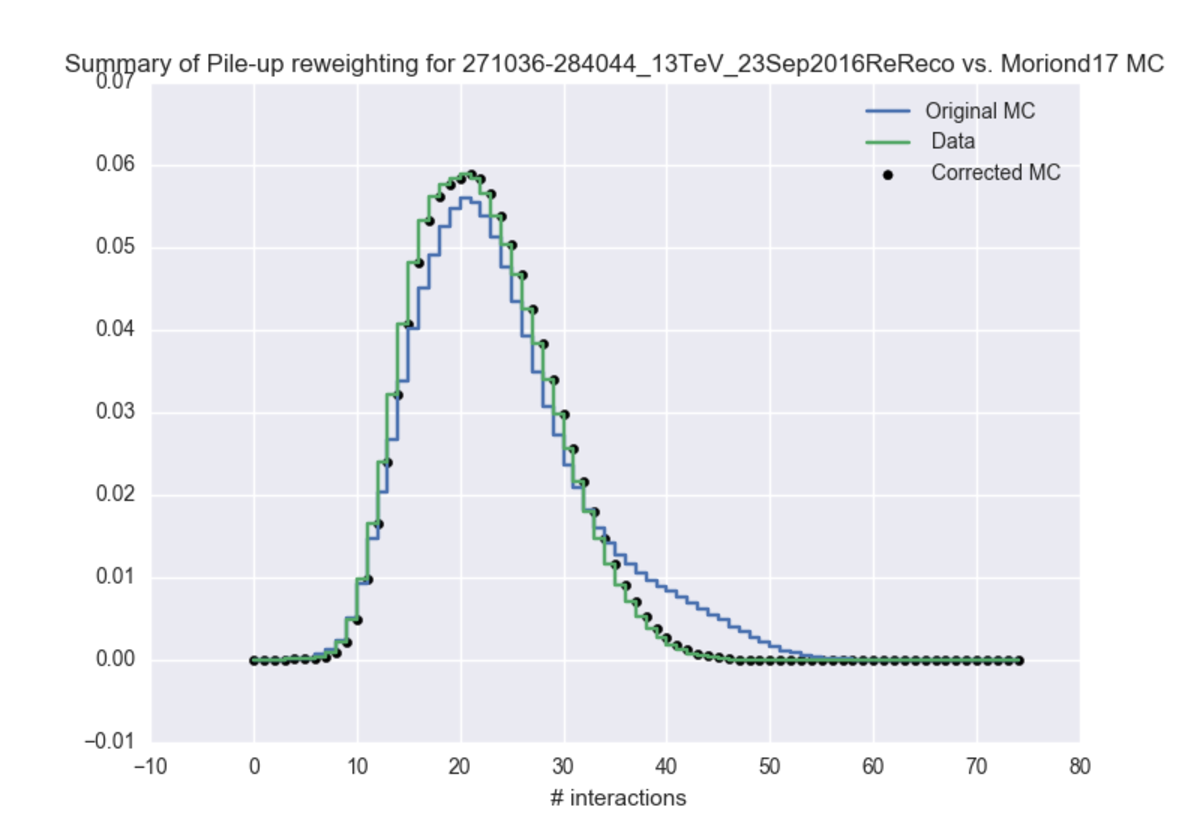
\includegraphics[width=0.5\textwidth]{figures/pileup_reweighting/summarized_data.pdf}} ~
  \subfigure[]{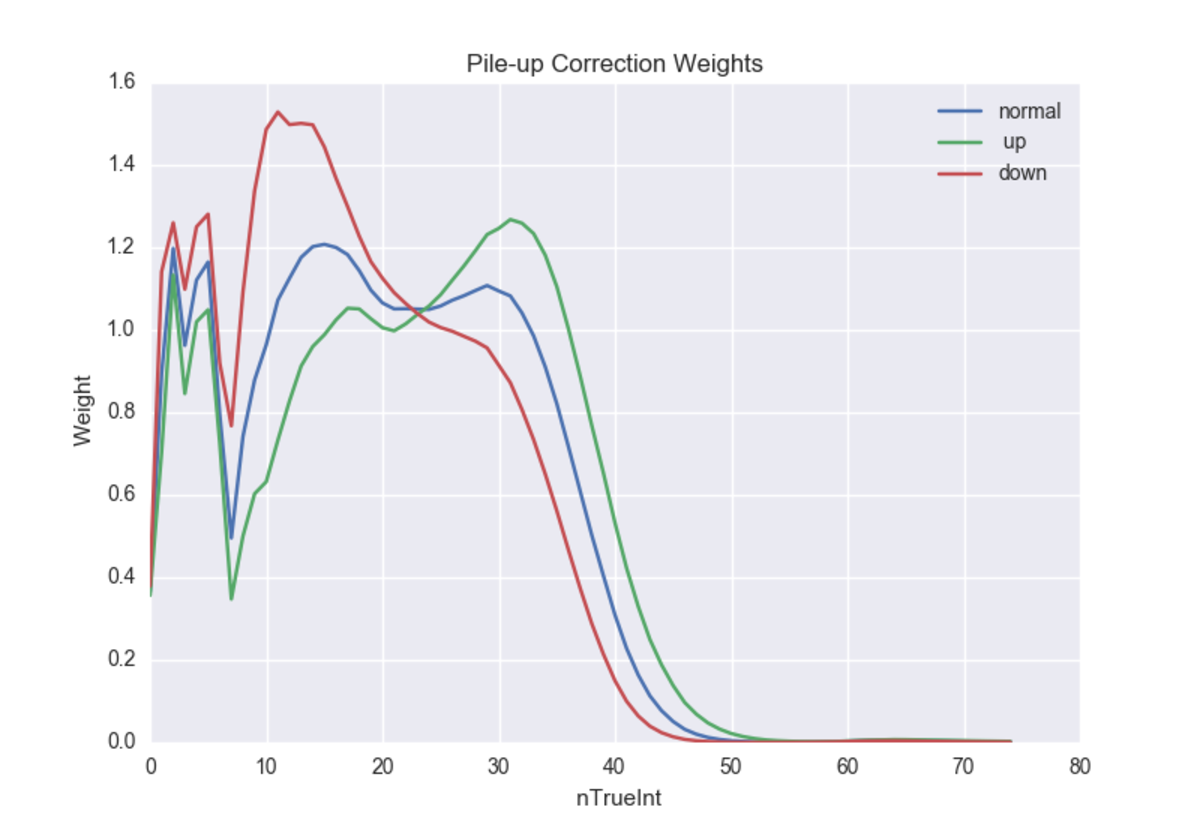
\includegraphics[width=0.5\textwidth]{figures/pileup_reweighting/tbl_20170125_01-tbl_corr_nTrueInt.pdf}} 
  \caption{(a) The distribution of the average numbers of the
    inelastic interactions per colliding bunch pair per lumi section
    in the data, corresponding distribution in the simulated events,
    and that of the reweighted simulated events. (b) The weights
    applied to simulated events as a function of the average number of
    the inelastic interactions per colliding bunch pair per lumi
    section.}
  \label{f044_corr_nTrueInt_data_mc_norm}
\end{figure}

Figure~\ref{f044_corr_nTrueInt_data_mc_norm} shows the distributions
of \verb!nTrueInt! in the data, simulated events and reweighted
simulated events. The figure demonstrates that the simulated events
have the distribution of \verb!nTrueInt! very similar to that found in
the data and after reweighting, the distributions from simulations
from data and simulation are identical.
%We note that the simulation does not contain events with 37 or more
%overlapping pp interactions, while the data do, causing the MC
%weighted distribution not to match perfectly the data. This small
%issue will be recovered once the new MC samples with updated PU
%profile will be available.

\subsubsection{Trigger efficiencies}
\label{sec:trigger-sf}

Simulated events in the signal region are corrected to account for
signal trigger inefficiencies. Simulated events in the muon control
regions rely on the use of an emulated muon trigger and the
application of data/MC scale factors to correct for differences in the
muon trigger efficiencies determined from data and simulation. Further
details are found in Sec.~\ref{sec:trigger}.

\subsubsection{Lepton and photon scale factors}

Simulation mismodelling of efficiencies related to object
identification and isolation requirements are mitigated by the use of
scale factors. Corrections related to trigger and tracking
reconstruction efficiencies are also considered. Typically, the scale
factors are near-unity and are determined by the POGs or the SUSY
lepton scale factor working group. We follow the SUSY Moriond17
recommendations, detailed here~\cite{susymoriond}. Further details are
given in later sections.

\subsubsection{Jet energy scale corrections and b-tag scale factors}
\label{sec:jecs-and-btag-sf}

Jet energy scale corrections and b-tag scale factors are applied to
the simulated event samples following the JetMET and BTV POG
recommendations. Details in subsequent sections. 

\subsubsection{Boson-\texorpdfstring{\Pt}{pT}-dependent NLO corrections}

The \MADGRAPH generator is used to simulate W + jets, DY + jets,
\znunu\ + jets, and \gj at leading order. Missing higher order
corrections, which can result in a modified boson \Pt distribution,
can be determined from (QCD) NLO simulation and (EWK) theory
calculations, as done by the the monojet search in the EXO
PAG~\cite{}. We apply these corrections to our simulated samples and
assume a 100\% uncertainty in these corrections, which is propagated
through the analysis and introduced to the likelihood model via a
dedicated nuisance. Further details are given in Sec.~\ref{sec:}.

\subsubsection{\texorpdfstring{\nisr}{Nisr} reweighting for \texorpdfstring{\ttbar}{TTbar}}
\label{sec:nisr}
 
To improve on the \MADGRAPH modelling of the multiplicity of
additional jets from initial state radiation (ISR), the SUSY group
recommends to reweight \MADGRAPH \ttbar Monte Carlo events according
to the number of ISR jets ($N_J^{ISR}$) identified in the event so as
to improve the jet multiplicity agreement with data. The reweighting
factors vary between 0.92 and 0.51 for $N_J^{ISR}$ between 1 and 6. In
this analysis, we categorise identically the events in the control and
signal regions according to the number of jets reconstructed in an
event. Hence such a correction is expected to have very little impact
on the final result. 

Further, this procedure attempts to correct for the mismodelling of
associated jet production for \ttbar processes, which may be due to
missing higher-order calculations in the LO \MADGRAPH MC. Hence, for
consistency with the V + jets samples (also produced with
\MADGRAPH{}@LO), we follow the recommendations of the SUSY group and
apply the $N_J^{ISR}$ corrections to our simulated samples. The
uncertainty is assumed to be 50\% of the corrections, which is
propagated through the analysis and introduced to the likelihood model
via a dedicated nuisance.

\subsection{Corrections to simulation for signal processes}

\fixme{IDENTIFY THE MAIN CORRECTIONS TO BE APPLIED, AS DETAILED IN THE
SUSY TWIKI}

%%____________________________________________________________________________||

%%____________________________________________________________________________||
\section{Trigger strategy}
\label{sec:triggers}

\subsection{Signal regions\label{sec:hadronic_signal_region}}

In Run~2, the RA1 analysis retains low thresholds comparable to those
used during Run~1 with developments to the trigger selection,
maintaining sensitivity to signatures of new physics with hadronic
energies as low as $\scalht = 200$ GeV. This in part is achieved by a
migration to PF-based jet reconstruction within the HLT which, in
conjunction with a reduction of clustering radius parameter $\Delta R
= 0.4$, provides improvements in jet energy resolution in high-pileup
conditions and mitigates the effects of pileup contamination within
the jet cone.

The RA1 analysis utilises a range of triggers for the selection of
events in the hadronic signal region to provide coverage over a wide
range of event topologies. A guiding principle of the analysis is to
be as inclusive as possible by maintaining low online and offline
thresholds. 

A suite of cross-triggers of the form
\verb!HLT_PFHTXXX_PFDijetAveYYY_AlphaT0pZZ!, comprising requirements
on \scalht, \alphat, and the average \pt of the leading two jets, are
used to record candidate signal events. The jets considered by these
cross-triggers satisfy $\Pt > 40\GeV$ and $|\eta| < 3.0$. A further
cross-trigger, \verb!HLT_PFMETNoMuXX_PFMHTNoMuXX_IDTight!  comprising
requirements on \MET, \HTmiss, and the presence of a jet with $|\eta|
< 3.0$, as well as a single-object \scalht trigger, are also employed
to record candidate signal events. The trigger requirements and
thresholds are summarised in
Table~\ref{tab:2015_Hadronic_Signal_Triggers}.

%The use of a \pt-averaged threshold of the two leading jets suppresses
%the QCD multijet background while providing acceptance to events
%exhibiting asymmetric jet topologies, such as monojet-like signatures
%of compressed spectrum and DM models. It was found that a dijet
%average threshold of 90 \GeV ensured the optimum performance when
%balancing efficiency and rate, with both the $\scalht$ and $\alphat$
%thresholds across all jet topologies. The dijet average requirement
%does however lead to a loss in efficiency for asymmetric jet events
%where the sub-leading jet is soft.
%This loss in efficiency is mitigated by taking the disjunction of the
%\alt and monojet triggers which provides a recovery of efficiency in
%the turn-on and close to the plateau for the low-\scalht asymmetric
%categories.  

%The Level-1 seeds for the $\scalht$--$\alphat$ HLT paths are given by
%the disjunction of all available hadronic scalar energy and missing
%energy sum seeds for the given run scenario. A loose calorimeter
%trigger prefilter is utilised to reduce the pass-through rate prior to
%track-based reconstruction, ensuring the PF-based filters meet timing
%requirements. The calorimeter prefilter utilises loose \scalht and
%dijet average \pt requirements in addition to a new variable \alphat',
%defined as \alphat in the limit $\Delta\scalht \rightarrow 0$, which
%better correlates \alphat between calorimeter and PF-based
%reconstruction.

%The choice of threshold for the \scalht--\alphat triggers were tuned
%to maintain acceptance for a range of signal topologies whilst
%effectively suppressing QCD multijet events to maintain acceptable
%trigger rates.

\begin{table}[h!]
  \topcaption{Summary of the L1 seeds and HLT trigger paths used by
    the analysis. 
    The lowest and highest (in parentheses) thresholds used for each
    HLT trigger path during the 2016 data taking period are given. 
  } 
  \footnotesize
  \centering
\begin{tabular}{ll} 
  \hline
  L1 seed & HLT path \\
  \hline
  {\scriptsize\verb!HTT or ETM!} & {\scriptsize\verb!HLT_PFHT200_PFDijetAve90_AlphaT0p57(65)!} \\
  {\scriptsize\verb!HTT or ETM!} & {\scriptsize\verb!HLT_PFHT250_PFDijetAve90_AlphaT0p55(57)!} \\
  {\scriptsize\verb!HTT or ETM!} & {\scriptsize\verb!HLT_PFHT300_PFDijetAve90_AlphaT0p53(55)!} \\
  {\scriptsize\verb!HTT or ETM!} & {\scriptsize\verb!HLT_PFHT350_PFDijetAve90_AlphaT0p52(53)!} \\
  {\scriptsize\verb!HTT or ETM!} & {\scriptsize\verb!HLT_PFHT400_PFDijetAve90_AlphaT0p51(52)!} \\
  {\scriptsize\verb!HTT!}        & {\scriptsize\verb!HLT_PFHT800(900)!} \\
  {\scriptsize\verb!ETM!}        & {\scriptsize\verb!HLT_PFMETNoMu90(110)_PFMHTNoMu90(110)_IDTight!} \\
  \hline
\end{tabular}
\label{tab:2015_Hadronic_Signal_Triggers}
\end{table}

The efficiency of the signal triggers are measured in data using event
samples containing an electron and muon, recorded with unprescaled
electron and muon ``reference'' triggers and defined by a
signal-region-like selection criteria (when ignoring the lepton in the
computation of event-level variables, such as \scalht or \MET). Biases
in these measurements can be introduced due to the contamination in
the computation of event-level variables and different treatments
between trigger and offline reconstructions, the degree of which
varies with \scalht and \njet. In the case of efficiency measurements
using the electron reference trigger, no cross-cleaning of electrons
from jets is performed offline, with the electron being included in
the computation of event-level jet energy sums, such as \scalht, \MHT
and \alt. When using the muon reference triggers, offline
cross-cleaning of the muons is performed. 

The trigger efficiency as a function of \mht for the full suite of
triggers, as determined from the data samples described above, is
shown per \scalht bin (following the \scalht binning scheme of the
signal region) in Fig.~\ref{fig:alphat_turnons} (in
Appendix~\ref{app:triggers}). The figure contains efficiency curves
determined from both the muon and electron event samples. Significant
differences are visible in the turn-on region, due to the
cross-cleaning issues through the various steps of the
trigger--analysis chain (L1, HLT Calo-based pre-filter, HLT PF-based
decision, offline) as described above. However, the efficiencies are
close to 100\% for the requirement $\HTmiss > 200\GeV$, as illustrated
by Table~\ref{tab:trigger-eff}, which is now the default \HTmiss
requirement used in this analysis. The measured efficiencies and their
uncertainties are applied as corrections to the MC samples. The
central value of the correction is taken from the efficiency measured
with the electron reference trigger. The statistical uncertainties in
the central values, as well as the difference in efficiencies between
those measured with the electron and muon triggers, are propagated.

\begin{table}[h!]
  \topcaption{Efficiency of the full suite of signal triggers as a
    function of \scalht after applying the signal region selection
    criteria, determined from $e$ + jets and \mj event samples.
  } 
  \footnotesize
  \centering
  \begin{tabular}{lcccc} 
    \hline
    Event sample & \multicolumn{4}{c}{\scalht bin [GeV]}                                                       \\
    \cline{2-5}
                 & 200--400             & 400--600             & 600--900              & $>$900                \\
    \hline
    $e$ + jets\T & $97.4^{+0.5}_{-0.6}$ & $97.9^{+0.8}_{-1.2}$ & $100.0^{+0.0}_{-1.8}$ & $100.0^{+0.0}_{-3.6}$ \\
    \mj\B        & $98.0^{+0.0}_{-0.0}$ & $98.9^{+0.0}_{-0.0}$ & $99.4^{+0.1}_{-0.1}$  & $99.9^{+0.0}_{-0.1}$  \\
    \hline
  \end{tabular}
  \label{tab:trigger-eff}
\end{table}

\begin{table}[H]
\caption{The luminosity collected by each HLT, or combination of Triggers, from the entire 2016 run. Over the course of the run, the threshold for the lowest unprescaled trigger in each category rose. The fraction of luminosity collected by each Trigger whilst it was lowest threshold is included.}
\resizebox{\textwidth}{!}{
\begin{tabular}{lp{0.25\linewidth}p{0.33\linewidth}}
  \hline
  Trigger & Luminosity collected (fb$^{-1}$) & Fraction collected as lowest unprescaled trigger \\
  \hline
  \texttt{HLT\_IsoMu22 or HLT\_IsoTkMu22} & 28.6 & 0.80 \\
  \texttt{HLT\_IsoMu24 or HLT\_IsoTkMu24} & 35.9 & 0.20 \\
  \hline
  \texttt{HLT\_PFHT800} & 27.3 & 0.76 \\
  \texttt{HLT\_PFHT900} & 35.9 & 0.24 \\
  \hline
  \texttt{HLT\_PFMETNoMu90\_PFMHTNoMu90\_IDTight} & 13.9 & 0.39 \\
  \texttt{HLT\_PFMETNoMu100\_PFMHTNoMu100\_IDTight} & 17.6 & 0.10 \\
  \texttt{HLT\_PFMETNoMu110\_PFMHTNoMu110\_IDTight} & 35.3 & 0.49 \\
  \texttt{HLT\_PFMETNoMu120\_PFMHTNoMu120\_IDTight} & 35.9 & 0.02 \\
  \hline
\end{tabular}
}
\end{table}

\subsection{Control regions\label{sec:control_samples}}

Samples of \mj and \mmj events are selected with the logical OR of the
\verb!HLT_IsoMu22!, \verb!HLT_IsoTkMu22!, \verb!HLT_IsoMu24! and
\verb!HLT_IsoTkMu24! triggers. The trigger efficiencies are provided
by the muon POG and are determined by the muon for both data and
simulated samples (containing a trigger emulation) using a tag and
probe method. The POG also provide data-to-simulation scale factors,
which we apply to the trigger-efficiency-corrected event yields from
simulation. The muon trigger efficiencies per (\njet, \nb, \scalht)
bin are determined for both the \mj and \mmj samples. For each bin,
the trigger efficiency values provided by the POG are weighted
according to \Pt and $\eta$ distributions of the muon(s) to give a
bin-averaged value. For the \mj sample, the efficiencies are typically
around 90\% and rather independent of \njet, \nb, and \scalht. For the
\mmj sample, the average efficiencies are $\sim99\%$ (as either muon
can provided the positive trigger decision). Statistical and
systematic uncertainties are propagated through via the scale factor
corrections, following the prescription from the muon POG.

A sample of \gj events is recorded with an \verb!OR! of the
\verb!HLT_Photon175! and \verb!HLT_ECALHT800! triggers. The efficiency
is measured as a function of both photon \Pt and \HTmiss for events in
the JetHT data set satisfying the \gj control region selection, as
shown in Fig.~\ref{fig:photon_turnons_photonPt}. The single photon
trigger alone exhibits a decreasing efficiency with increasing photon
\Pt, which is attributed to an H/E cut at Level 1. The inefficiency
can be largely recovered by also employing the \verb!ECALHT800!
trigger. In this way, the inefficiency can be recovered for photon
$\Pt > 600\GeV$. The photon efficiency is $\sim 98\%$. The
efficiencies are used to correct the simulated event counts in the \gj
sample, and a systematic uncertainty is assumed to be the magnitude of
the inefficiency ($\sim 2\%$).

%A sample of QCD multijet events is recorded with the same trigger
%requirements used for the signal region, summarised in
%Table~\ref{tab:2015_Hadronic_Signal_Triggers}. The trigger efficiency
%is determined from data using a sample of \gj events in which the
%photon is treated as a jet. 
%This sample is recorded with the \verb!HLT_Photon175! and
%\verb!HLT_ECALHT800! triggers.
%\fixme{QCD SIDEBAND TRIGGER EFF PLOTS?}

%%____________________________________________________________________________||

%%____________________________________________________________________________||
\section{Physics objects}
\label{sec:objects}

The definitions of the physics objects used in this analysis follow
the recommendations of the various Physics Object Groups (POGs).
During data taking these recommendations are subject to change and
will be be updated if necessary.

\subsection{Jets}
\label{sec:jetreco}

Jets are defined as sets of particle-flow (PF) candidates clustered by
the anti-$k_{T}$ jet clustering algorithm \cite{Cacciari:2008gp} with
a distance parameter of 0.4 (PFJets). Charged Hadron Subtraction (CHS)
is applied, i.e., charged hadrons that can be traced back to pileup
vertices are not clustered.  The four-momenta of jets are initially
defined as the four-vector sum of the four-momenta of the constituent
particle-flow candidates and then scaled by the jet energy correction
factors designated as L1FastJet, L2Relative, and L3Absolute
\cite{Chatrchyan:2011ds}.

The ``loose'' working point Jet-Id selection criteria is chosen.  The
cuts are listed in Tab.~\ref{tab:loose-jet-id}.  In addition, a
dedicated selection is applied to reject ``beam halo'' candidate
events, as described in Section~\ref{sec:had-signal}.

\begin{table}[ht!]
  \caption{The ``loose'' jet ID requirements. \label{tab:loose-jet-id}}
  \centering
  \begin{tabular}{ ccc }
    \hline
    \hline
    Variable & cut & notes \\ \hline
    \multicolumn{3}{c}{$-3.0 < \eta_{\mathrm{jet}} < 3.0$} \\ \hline    
    Neutral Hadron Fraction & $<0.99$ & - \\
    Neutral EM Fraction & $<0.99$ & - \\
    Number of constituents & $>1$ & - \\
    Charged Hadron Fraction & $>0$ & only for $|\eta_{\mathrm{jet}}| < 2.4$ \\
    Charged Multiplicity & $>0$ & only for $|\eta_{\mathrm{jet}}| < 2.4$ \\
    Charged EM Fraction & $<0.99$ & only for $|\eta_{\mathrm{jet}}| < 2.4$ \\ \hline
    \multicolumn{3}{c}{$|\eta_{\mathrm{jet}}| > 3.0$} \\ \hline        
    Neutral EM Fraction & $<0.90$ & - \\
    Number of Neutral Particles & $>10$ & - \\
    \hline
    \hline
  \end{tabular}
\end{table}

\subsection{b-tagged jets}
\label{sec:btags}

Jets originating from bottom quarks are identified through vertices
that are displaced with respect to the primary interaction
\cite{Chatrchyan:2012jua}.  The algorithm used to tag b-jets is the
Combined Secondary Vertex tagger V2, with the ``medium'' working
point, which is achieved by requiring a cut of $>$ 0.800 on the
algorithm discriminator variable.  This results in a gluon/light-quark
mis-tag rate of $\sim$1 \% (where ``light'' means $u$, $d$ and $s$
quarks), a charm-quark mis-tag rate of $\sim$10 \% and a b-quark b-tag
efficiency of about 60 \%.

Some validation studies used by the analysis make use of the ``loose''
and ``tight'' working points, which are defined by the thresholds
requirements of 0.460 and 0.935 on the discriminator variable. These
requirements yield light-flavour mistag probabilities of $\sim$10 and
$\sim$0.1\%, respectively.

\subsection{Muons}
\label{sec:muon-id}

\subsubsection{Selection}

Muons are selected in the \mj and \mmj control regions using the
``tight'' working point definition of the recommended identification
algorithm from the Muon POG.  Muons are also required to be well
isolated, i.e. a low activity within a cone defined by $\deltaR < 0.3$
around the muon trajectory. The transverse momenta of PF neutral and
charged candidates, as well as photons, lying within the cone around
the lepton are summed. The relative combined isolation
$I^\mathrm{rel}_\mathrm{comb}$ is then defined as the ratio of this
scalar sum to the transverse momentum of the lepton
candidate. Additionally, $\rho\times \mathcal{A}_\textrm{eff}$
corrections are applied to remove the effects of pileup.  Muons are
defined to be isolated if they fulfill the criterium
$I^\mathrm{rel}_\mathrm{comb} < 0.15$.

\subsubsection{Veto}

For the purpose of vetoing muons in the signal region, the ``loose''
working point is used, which provides $\sim$ 98 $\%$ efficiency.  In
the hadronic signal region a variable cone size for the isolation is
used, which is referred to as ``mini-isolation''.  This isolation
algorithm helps in recovering some efficiency in the lepton selection
for boosted topology of top quark decays, in which the muon's track
may be found close to the jet activity due to the boost of the parent
top.  Therefore, the cone size used for the calculation of the lepton
isolation is reduced as a function of the lepton \Pt, as follows:
$R=0.2$ for $\Pt_{\ell}\leq50\gev$, $R=10\gev/\Pt_{\ell}$ for $50 \gev
< \Pt_{\ell} < 200\gev$ and $R=0.05$ for $\Pt_{\ell} > 200 \gev$.  In
the signal region, identified muons with mini-isolation satisfying
$I^\mathrm{min}_\mathrm{comb} < 0.2$ are vetoed.

\subsection{Photons}
\label{sec:photon-id}

\begin{table}[ht!]
  \caption{Photon identification.\label{tab:photon-id-gamma}}
  \centering
  \footnotesize
  \begin{tabular}{ ccc }
    \hline
    \hline
    Categories & \multicolumn{2}{c}{Barrel}   \\
    Working point  & Tight & Loose \\
    \hline
    Conversion safe electron veto & Yes & Yes  \\
    Single Tower H/E              & 0.05 & 0.05  \\
    $\sigma_{i\eta i\eta}$        & 0.0100 & 0.0102 \\
    PF charged hadron isolation   & 0.76 & 3.32  \\
    PF neutral hadron isolation   & 0.97 + 0.014 $\times$ $p_{\mathrm{T},\gamma}$ + 0.000019 $\times$ $p_{\mathrm{T},\gamma}^{2}$ & 1.92 + 0.014 $\times$ $p_{\mathrm{T},\gamma}$ + 0.000019 $\times$ $p_{\mathrm{T},\gamma}^{2}$  \\
    PF photon isolation           & 0.08 + 0.0053 $\times$ $p_{\mathrm{T},\gamma}$ & 0.81 + 0.0053 $\times$ $p_{\mathrm{T},\gamma}$ \\
    \hline
    \hline
    Categories & \multicolumn{2}{c}{Endcap}   \\
    Working point  & Tight & Loose \\
    \hline
    Conversion safe electron veto & Yes & Yes  \\
    Single Tower H/E              & 0.05 & 0.05  \\
    $\sigma_{i\eta i\eta}$        & 0.0268 & 0.0274 \\
    PF charged hadron isolation   & 0.56 & 1.97  \\
    PF neutral hadron isolation   & 2.09 + 0.014 $\times$ $p_{\mathrm{T},\gamma}$ + 0.000025 $\times$ $p_{\mathrm{T},\gamma}^{2}$ & 11.86 + 0.014 $\times$ $p_{\mathrm{T},\gamma}$ + 0.000025 $\times$ $p_{\mathrm{T},\gamma}^{2}$ \\
    PF photon isolation           &  0.16 + 0.0034 $\times$ $p_{\mathrm{T},\gamma}$ & 0.83 + 0.0034 $\times$ $p_{\mathrm{T},\gamma}$ \\
    \hline
    \hline
  \end{tabular}
  \end{table}

\subsubsection{Selection}

Photons are identified according to the ``tight'' working point
definition ($\sim$ 71 $\%$ efficiency) of the simple cut-based photon
identification algorithm \cite{photon-id} and required to be well
isolated.  A PF-based isolation is used with a cone size $\Delta R$
$<$ 0.3 and $\rho\times \mathcal{A}_\textrm{eff}$ corrections are applied to remove the
effects of pileup \cite{pf-photon}.  Table \ref{tab:photon-id-gamma}
summarises the identification and isolation selection used.

\subsubsection{Veto}

Photons are vetoed in the definition of the hadronic signal region and
muon control regions, as described in Sec.~\ref{sec:preSelection},
while a control region with one photon (``\gj'') is defined for the
purpose of the background estimation, as described in
Sec.~\ref{sec:photoncontrolSelection}.


\subsection{Electrons}
\label{sec:electron-id}

\begin{table}[h!]
  \caption{Electron identification for veto (``loose'' working point).\label{tab:ele-id}}
  \centering
  \footnotesize
  \begin{tabular}{ lcc }
    \hline
    \hline
    Categories                                               & Barrel    & EndCap    \\
    \hline
    $\Delta \eta_{In}$                                       & 0.0105   & 0.00814  \\
    $\Delta \phi_{In}$                                       & 0.115    & 0.182  \\
    $\sigma_{i\eta i\eta}$                                   & 0.0103    & 0.0301  \\
    H/E                                                      & 0.104    & 0.0897   \\
    d0 (vtx)                                                 & 0.0261    & 0.118  \\
    dZ (vtx)                                                 & 0.041    & 0.822  \\
    $\lvert(1/E_{\textrm{ECAL}} - 1/p_{\textrm{trk}})\rvert$ & 0.102     & 0.126  \\
    Missing hits (inner tracker)                             & 2         & 1         \\
    Conversion veto                                          & yes       & yes   \\
    \hline
    \hline
  \end{tabular}
\end{table}

\subsubsection{Selection}

Electron-based control regions are not used by this analysis. 

\subsubsection{Veto}

In order to veto electrons in the hadronic signal region and the muon
and photon control regions, the ``loose'' working point definition
($\sim$ 90 $\%$ efficiency) of the cut-based electron identification
\cite{electron-id} is used.  Electrons are also required to be
isolated.  Similar to muons, in the hadronic signal regions a PF-based
isolation \cite{pf-photon} is used with a cone size determined by the
mini isolation algorithm (see Sec.~\ref{sec:muon-id}) and $\rho\times
\mathcal{A}_\textrm{eff}$ corrections are applied to remove the effects of pileup.
Isolated electrons are defined by $I^\mathrm{min}_\mathrm{comb} < 0.1$.

Table \ref{tab:ele-id} summarises the identification requirements. 

\subsection{Single isolated tracks}
\label{sec:SIT}

\subsubsection{Selection}

Event samples containing only a single isolated track (and no leptons)
are not used by this analysis, other than for ``closure test''
studies, see Sec.~\ref{sec:}. In this case, the veto definition below
is simply inverted.

\subsubsection{Veto}

A single isolated track (SIT) can be used to identify W bosons through
their leptonic decays: W $\rightarrow$ $\mu \nu$, W $\rightarrow$
$e\nu$, and W $\rightarrow$ $\tau$($\rightarrow l\nu$) $\nu$.  Single
prong decays of the tau lepton can also be identified: W $\rightarrow$
$\tau$ ($\rightarrow$ h$^{\pm}$ + n$\pi^{0}\nu$) $\nu$.  A single
isolated track comprises a charged PF candidate with $\Pt > 10 \gev$,
$\Delta z(\mathrm{track}, \mathrm{PV}) < 0.05 \, \mathrm{cm}$ and with
a relative isolation smaller than 0.1, where the isolation is
determined from the sum of the \Pt of the charged PF candidates within
$\Delta R < 0.3$.

\subsection{Missing transverse momentum}

As indicated in Sec.~\ref{sec:}, the transverse momentum imbalance of
an event (\met) is defined as the magnitude of the vector sum of the
transverse momentum of all particle-flow candidates in the event.

The Type-I \met correction \cite{Khachatryan:2014gga} is applied, \ie
the transverse momentum of the particle-flow candidates clustered as
jets are replaced with the transverse momentum of the jets that are
scaled by the jet energy correction factors.

The \met is used in the definition of the transverse mass, $M_{T}$,
which is in turn used as part of the selection criteria that define
the single muon control sample (Sec.~\ref{sec:mucontrolSelection}),
and for the $\mhtmet$ cleaning filter, as described in
Sec.~\ref{sec:selection}.

%%____________________________________________________________________________||

%____________________________________________________________________________||
\section{Event selection and categorisation}
\label{sec:selection}

This section first outlines the set of ``pre-selection'' requirements
that are common to all signal and control regions, before defining the
selection criteria that are specific to each region.

%%____________________________________________________________________________||
\subsection{Common pre-selection requirements}
\label{sec:preSelection}

The event selection criteria described in this section are common to
all signal and control regions. These selections are summarised in
Table~\ref{tab:pre-selections} and described in further detail below.

\begin{table}[h!]
  \topcaption{Summary of the pre-selection criteria.}
  \label{tab:pre-selections}
  \centering
  \small
  \begin{tabular}{ ll }
    \hline
    \ETmiss quality               & Filters related to beam and instrumental effects, and reconstruction failures                               \\
                                  & \parbox[t]{12cm}{
                                    (Primary Vertex, 
                                    CSC Beam Halo,
                                    HBHE Noise and Isolation,                                                                                   \\
                                    ECAL Endcap SC Noise, 
                                    ECAL TP, 
                                    Bad Muon, 
                                    Bad Charged Hadron)}                                                                                        \\
    Beam halo                     & $0.1 < \mathrm{CHF} < 0.95$ for highest-\Pt jet                                                             \\
    Jet $\mathrm{j}_i$ acceptance & Each jet $\mathrm{j}_i$ that satisfies $\pt^{\mathrm{j}_i} > 40\GeV$ and $\abs{\eta^{\mathrm{j_1}}} < 2.4$ \\
    Jet $\mathrm{j_1}$ acceptance & $\pt^{\mathrm{j_1}} > 100\GeV$                                                                              \\
    Jets below threshold          & $\HTmiss / \ETmiss < 1.25$                                                                                  \\
    Forward jet veto              & Veto events containing a jet satisfying $\pt > 40\GeV$ and $\abs{\eta} > 2.4$                               \\
    Energy sums                   & $\scalht > 200\GeV$ and $\HTmiss > 130\GeV$                                                                 \\
    \hline
  \end{tabular}
\end{table}

\subsubsection{MET filters}

A number of beam- and detector-related effects can induce significant
\met. Examples include beam halo, reconstruction failures, spurious
detector noise, or event misreconstruction due to detector
inefficiencies. These events, with large, non-physical values of \met,
are rejected with high efficiency by applying a range of dedicated
vetoes. All ``MET filters'' recommended by the JetMET POG and SUSY PAG
are applied by default in this analysis and listed in
Table~\ref{tab:pre-selections}.

\subsubsection{Charged hadron fraction (CHF) for leading jet}

In addition to the MET filters, a dedicated filter is applied to
remove beam halo, given that the CSC beam halo filter has been found
to be less efficient during the early Run 2 data-taking period
compared to the previous run.

Beam halo events manifest themselves as single energy deposits in the
calorimeters, which introduces large amounts of ``fake'' \met. This
effect is especially prominent in low-\njet events that satisfy the
signal region requirements, particularly at $\phi$ coordinates of 0
and $\pi$ because of the tendency of halo particles to lie within the
plane of the LHC ring.

Such spurious events are suppressed by requiring at least 10\% of 
the highest-\Pt jet's energy to originate from charged
hadrons. The effectiveness of this charged hadron fraction (CHF)
requirement is demonstrated in Fig.~\ref{fig:leadJetCleaning}.

Further, a requirement of $\mathrm{CHF} < 0.95$ for the highest-\Pt
jet removes events that contain reconstruction failures concerning
muons, which are prevelant in simulated multijet events.

%There is no need for this selection in the control regions, as the
%requirement of well identified physics objects, like muons and photons
%naturally removes spurious events of this kind.

The requirement $0.1 < \mathrm{CHF} < 0.95$ for the highest-\Pt jet
can be regarded as an additional jet ID requirement employed by this
analysis, with efficiency close to unity for real jets and thus not
affecting the signal efficiency significantly.

\begin{figure}[h!]
    \begin{center}
        {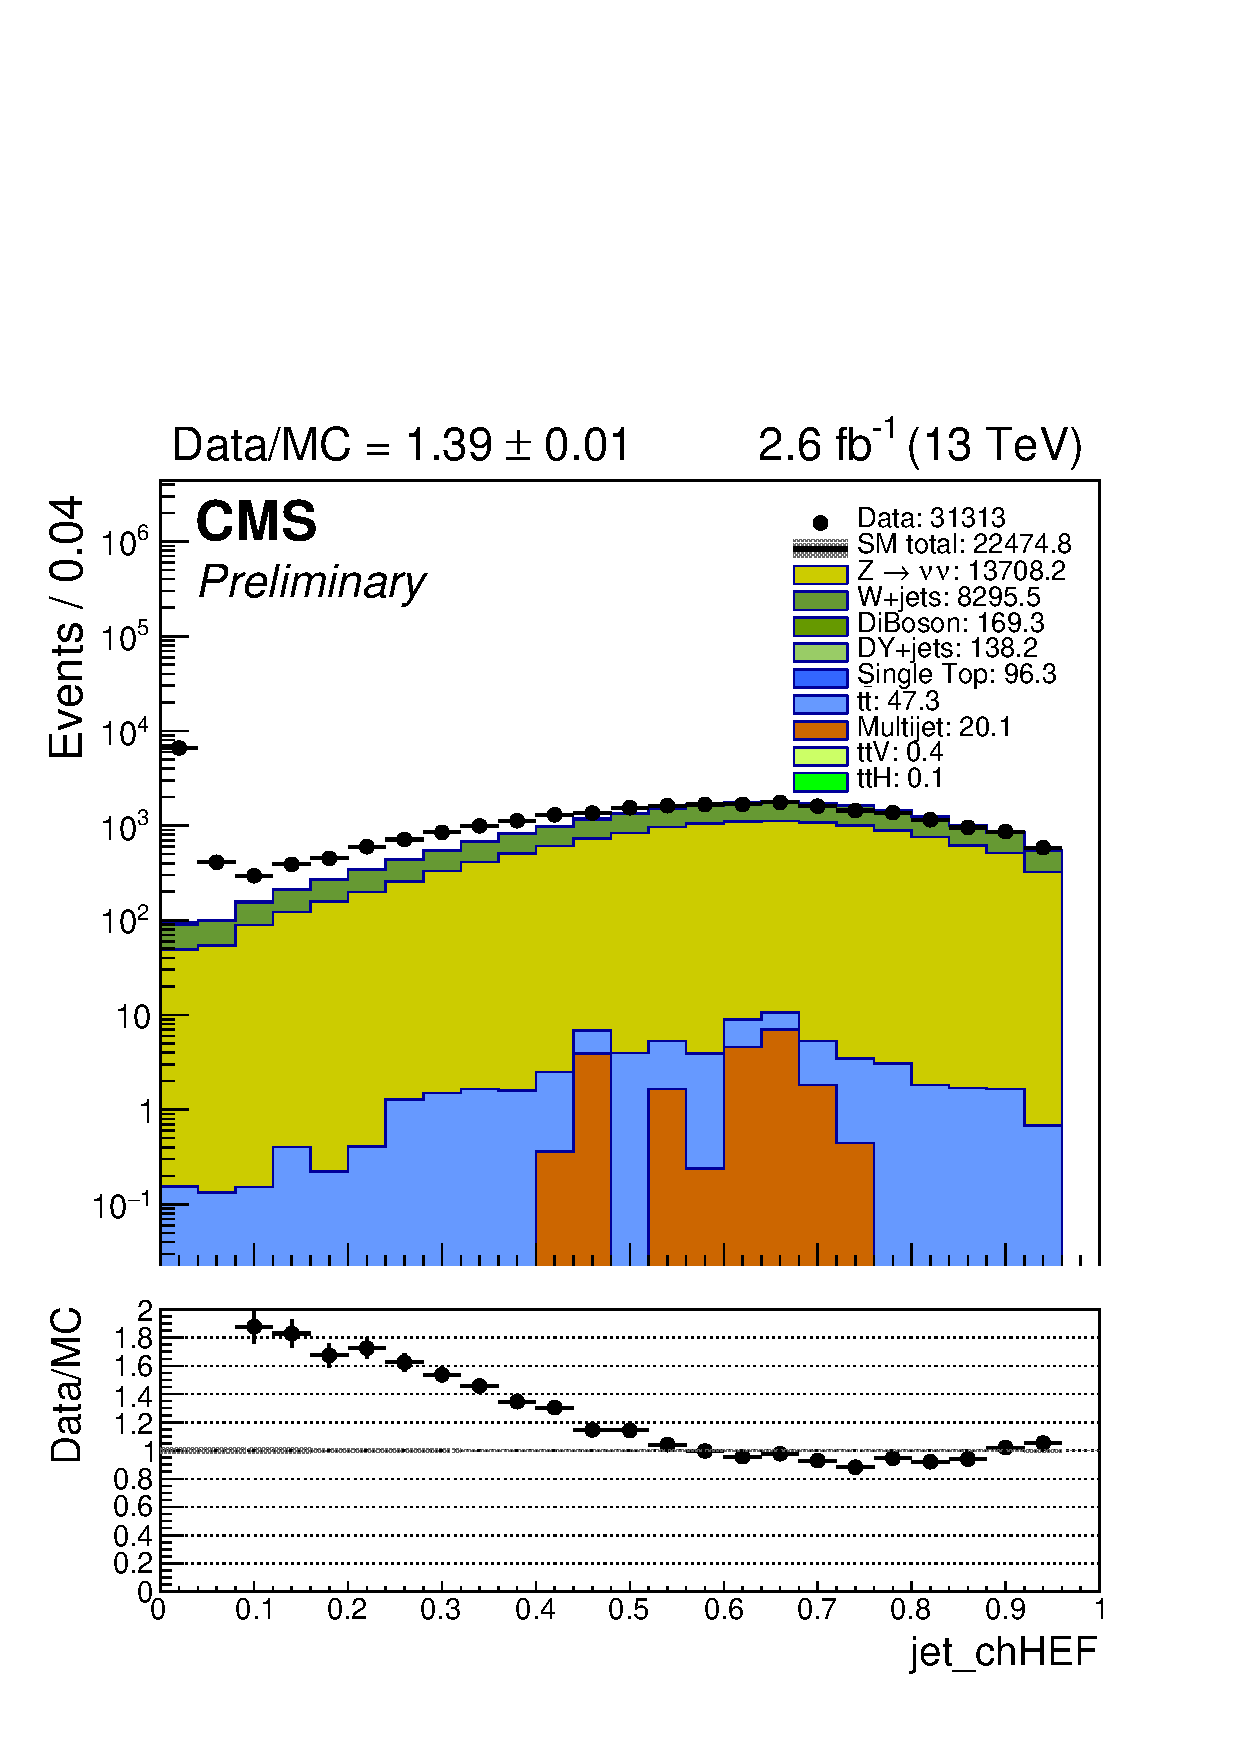
\includegraphics[width=0.32\textwidth]{figures/selection/jet_chHEF_mono_all_before.pdf}}
        {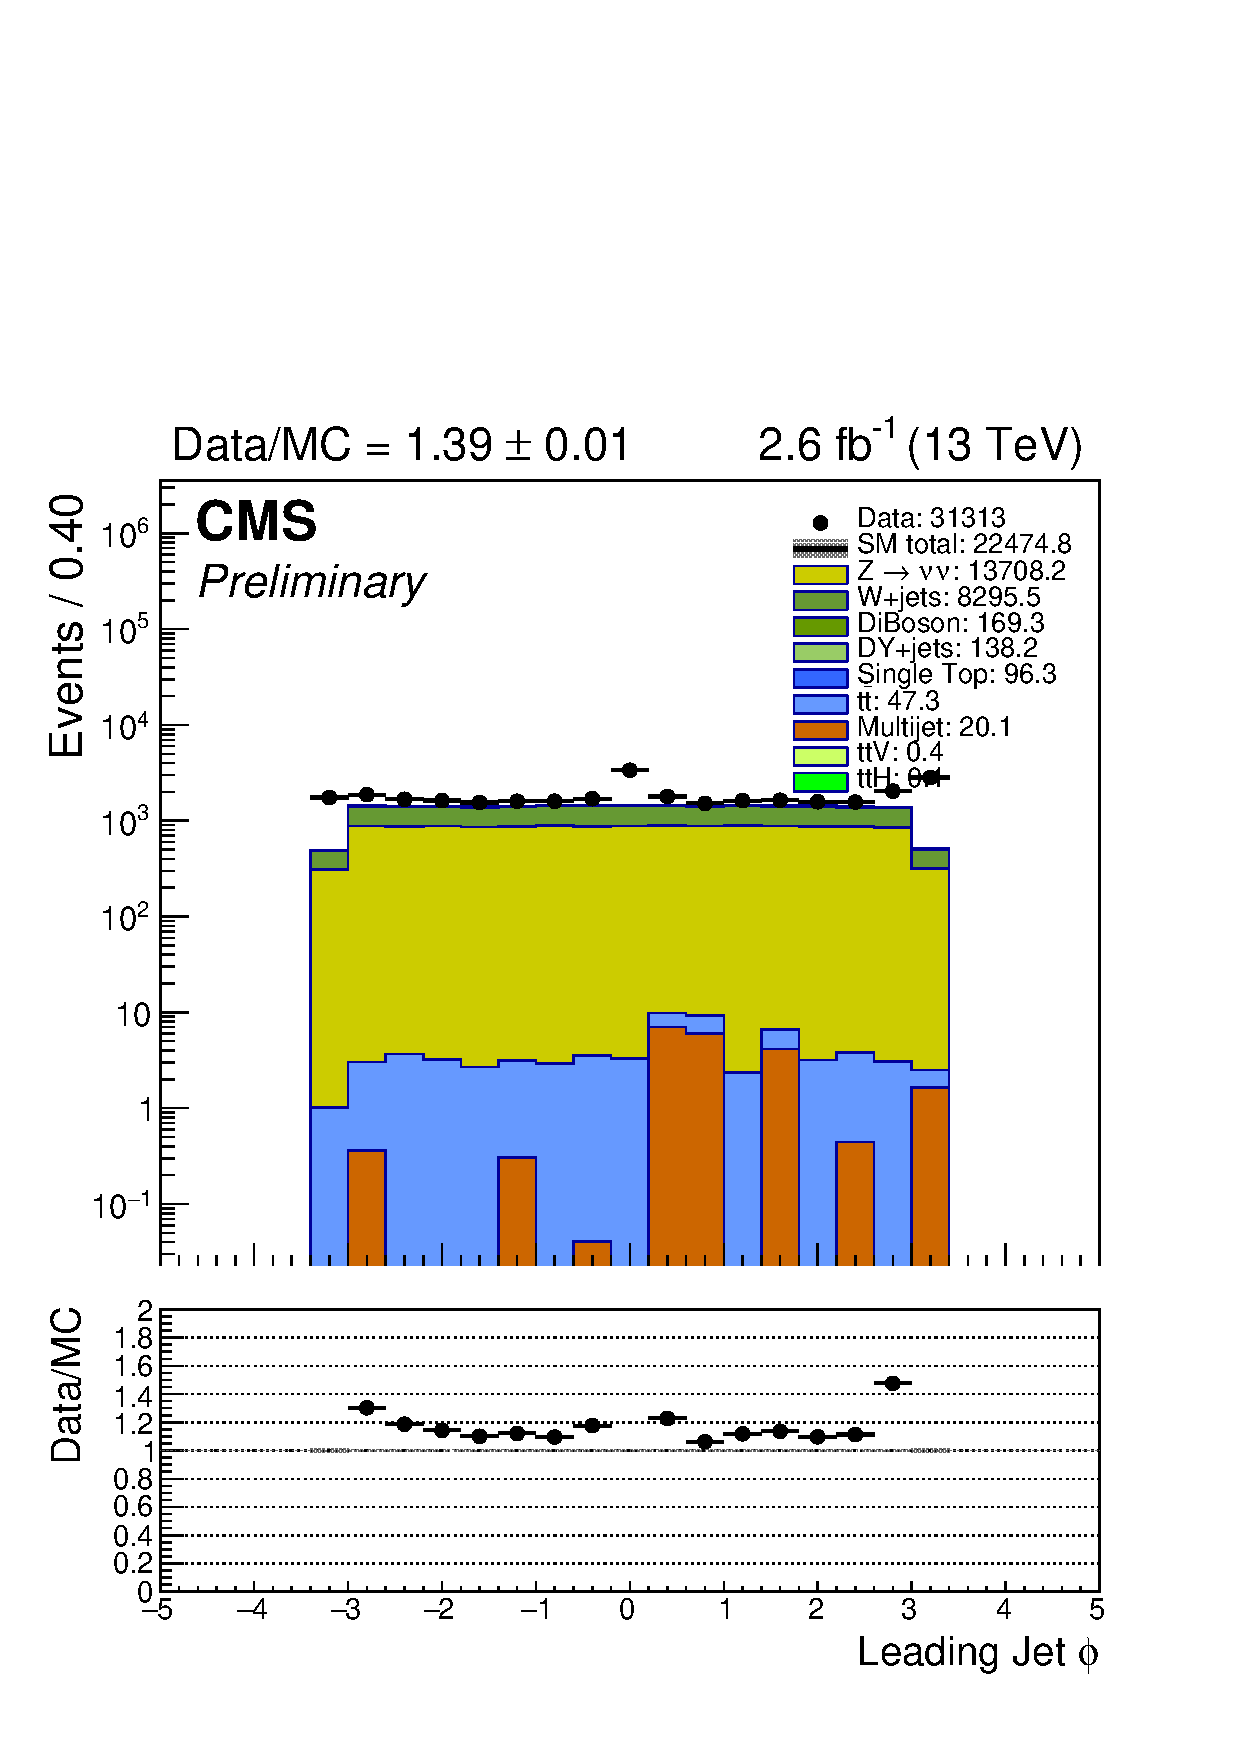
\includegraphics[width=0.32\textwidth]{figures/selection/jet_phi[0]_mono_all_before.pdf}}
        {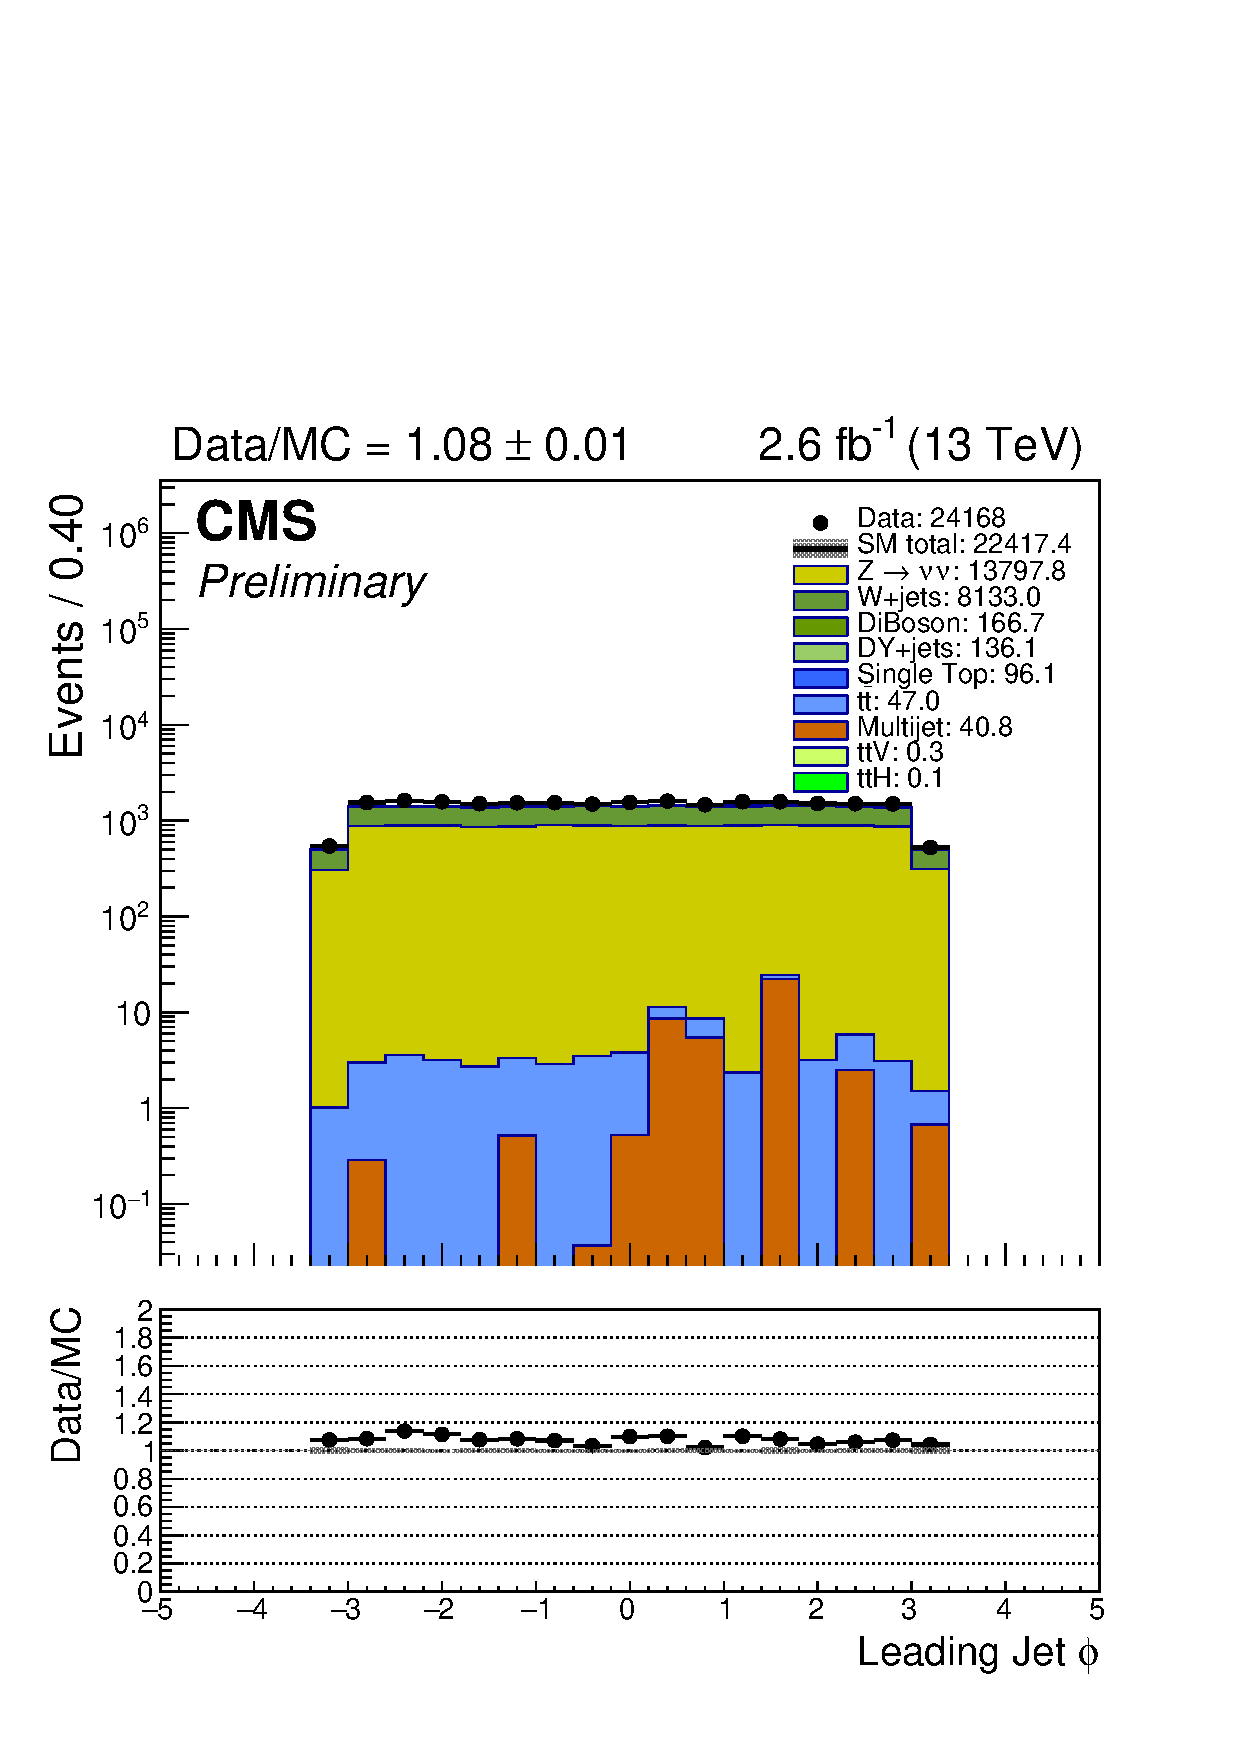
\includegraphics[width=0.32\textwidth]{figures/selection/jet_phi[0]_mono_all_after.pdf}}
        \caption{Distributions in the signal region of (Left) the jet
          charged hadron energy fraction (CHF), (Centre) the jet
          $\phi$ direction, and (Right) jet $\phi$ direction after
          applying a requirement of {CHF~$>0.1$}. The large excess in
          data at charged hadron fractions close to zero and ${\phi =
            0, \pi}$ is consistent with beam halo effects, and is
          effectively suppressed by the aforementioned selection.}
        \label{fig:leadJetCleaning}
    \end{center}
\end{figure}

\subsubsection{Experimental acceptance for jets}

Jets considered in the analysis are required to satisfy $\PT > 40\gev$
and $|\eta| < 2.4$. The selected jets are used in the calculation of
all jet-based event-level variables, such as \njet, \HT, \mht, and
\alphat (see Sec.~\ref{sec:} for their definitions).

The highest-\Pt jet in the event is required to satisfy $\Pt^{\mathrm
  j_1} > 100\gev$. This helps to ensure high trigger efficiencies
while maintaining high efficiency for a broad range of signal models.

Events are classified based on the second highest-\Pt jet, as
described in Sec.~\ref{sec:subleading-jet}.

\subsubsection{The \texorpdfstring{\mht/\met}{HTmiss/ETmiss} variable} 
\label{sec:mhtmet}

The value of \mht is compared to the missing transverse energy
variable, $\met$. Only events that satisfy
$R_{\mathrm{miss}}=\mht/\met < 1.25$ are considered in order to
protect against events containing multiple jets outside the
experimental acceptance (\eg ``below'' the \Pt acceptance) that
contribute significantly to \mht. In the case of the control regions,
in which well-reconstructed, isolated muons and photons are selected,
the $R_{\mathrm{miss}} < 1.25$ requirement is also applied. The \mht
sum does not consider the transverse momentum of the muons or
photon. Hence their momenta are also excluded from the \met sum, such that the
\mht and \met can be considered on an equal footing.

\subsubsection{The forward jet veto} 

Events containing jets in the forward region that satisfy the
requirements $\Pt > 40\gev$ and $|\eta|>2.4$ are rejected (regardless
of the identification requirement) to control background contributions
from SM processes such as multijet production, without introducing a
significant reduction in signal acceptance.

\subsubsection{Jet-based energy sums}

Events are required to have significant hadronic activity by requiring
$\scalht > 200\GeV$. Despite an increase in both multijet production
cross sections and pileup in Run~2, the lowest \HT threshold is kept
at the same value of the Run~1 analysis~\cite{Chatrchyan:2013lya} in
order to maintain acceptance to DM models or compressed SUSY.

Events are required to have appreciable missing transverse energy by
requiring $\mht>200\gev$.\footnote{This differs with respect to the
  previous iteration of the analysis, the ICHEP prelimary
  result~\cite{CMS-PAS-SUS-16-016}, which used $\HTmiss >
  130\GeV$. This change is motivated through studies that demonstrate
  a lack of knowledge of the trigger efficiency in the turn on of the
  efficiency curve, prior to the efficiency plateau at $\HTmiss
  \approx 200\GeV$.}  This requirement is applied to events in the
signal and control regions. The \scalht-dependent \alphat thresholds,
required to suppress multijet events as outlined in
Sec.~\ref{sec:had-signal}, provide an effective threshold on \mht in
the range 130--200\GeV, via the relationship in
Eq.~(\ref{eq:alphat3}). Hence, the extrapolation from control to
signal region in terms of the \alphat requirement for the signal
region (that is not required for the control regions, see below) is
minimised.

\subsection{The signal region}
\label{sec:had-signal}

The event selection criteria specific to the signal region are
described in this section and summarised in
Table~\ref{tab:sr-selections}.

\begin{table}[!h]
  \topcaption{Summary of the event selection criteria for the signal
    region. The criteria are applied in addition to the pre-selection
    requirements listed in Table~\ref{tab:pre-selections}.
  }
  \label{tab:sr-selections}
  \centering
  \begin{tabular}{ ll }
    \hline
    Lepton vetoes              & $\pt > 10\GeV$ and $\abs{\eta} < 2.5$ for isolated muons and electrons                          \\
    Single isolated track veto & $\pt > 10\GeV$  and $\abs{\eta} < 2.5$ for isolated tracks                                      \\
    Photon veto                & $\pt > 25\GeV$ and $\abs{\eta} < 2.5$ for isolated photons                                      \\
    QCD multijet rejection     & $\alphat > \mathrm{threshold}$ (\scalht-dependent, see Table~\ref{tab:alphat-thresholds} below) \\
    QCD multijet rejection     & $\bdphi > 0.5$ ($\njet \geq 2$) or $\bdphimod > 0.5$ ($\njet = 1$)                              \\[0.5ex]
    \hline
  \end{tabular}
\end{table}

\subsubsection{Lepton, photon, and single isolated track vetoes}
\label{sec:vetoes}

Using the identification criteria described in Sec.~\ref{sec:objects},
the following objects are vetoed when selecting events for the
hadronic signal region:
\begin{itemize}
\item muons with $\pt>10\,\mathrm{GeV}$ and $|\eta|<2.5$;
\item electrons with $\pt>10\,\mathrm{GeV}$ and $|\eta|<2.5$;
\item single isolated tracks with $\pt>10\,\mathrm{GeV}$ and
  $|\eta|<2.5$;
\item photons with $\pt>25\,\mathrm{GeV}$ and $|\eta|<2.5$;
\end{itemize}

\subsubsection{\texorpdfstring{\scalht}{HT}-dependent \texorpdfstring{\alphat}{AlphaT} requirements}
\label{sec:HT-AT-selection}

After the pre-selection criteria and the vetoes are applied, the
multijet background is still several orders of magnitude larger than
the typical signal expected from SUSY. Background events from multijet
production populate the region $\alphat \lesssim 0.5$ and therefore
can be rejected with very high efficiency by requiring events to
exhibit an \alphat value above an appropriate
threshold. Sec.~\ref{sec:alphatdef} defines the \alphat variable.

The \alphat thresholds are also chosen in order to ensure a trigger
efficiency close to unity in all the bins. More details on the trigger
strategy can be found in Sec.~\ref{sec:triggers}.

\begin{table}[h!]
  \caption{\alphat thresholds versus
    lower bound of \scalht bin. For all \HT bins satisfying $\HT >
    900\gev$, no \alphat cut is applied, and similarly for events with
     $\njet = 1$ (``monojet'' events, see
    Sec.~\ref{sec:subleading-jet}). Also
    shown is the flat \bdphi requirement
    (Sec.~\ref{sec:bdphi-selection}).}   
  \label{tab:alphat-thresholds}
  \centering
  \begin{tabular}{ lcccccccc }
    \hline
    \scalht [GeV]     & 200--250 & 250--300 & 300--350 & 350--400 & 400--900 & 900--1200 & $>$1200 \\
    \alphat threshold & 0.65     & 0.60     & 0.55     & 0.53     & 0.52     & (none)    & (none)  \\
    \bdphi threshold  & 0.5      & 0.5      & 0.5      & 0.5      & 0.5      & 0.5       & 0.5     \\
    \hline
  \end{tabular}
\end{table}

Table~\ref{tab:alphat-thresholds} summarises the \alphat thresholds
for each \HT bin. The \alphat threshold is dependent only on \HT and
not on \njet nor \nb that are used to define the event categories. No
\alphat cut is applied for events satisfying $\njet = 1$ (``monojet''
events, see Sec.~\ref{sec:subleading-jet}), as the variable is defined
only for $\njet \geq 2$. Further, no requirement is made for events
satisfying $\scalht > 1200\GeV$.

\subsubsection{\texorpdfstring{\bdphi}{biased dPhi} requirement} 
\label{sec:bdphi-selection}

Candidate signal events with two or more jets are accepted only if
they satisfy $\bdphi > 0.5$. This threshold is independent of \scalht,
unlike the \alphat requirement described above, as summarised in
Table~\ref{tab:alphat-thresholds}. In the case of events satisfying
$\njet = 1$ (``monojet'' events, see Sec.~\ref{sec:subleading-jet}),
the requirement $\bdphimod > 0.5$ must be satisfied. The definitions
of \bdphi and \bdphimod can be found in Sec.~\ref{sec:bdphi-def}. 

\subsection{The control regions}
\label{sec:control-region-selection}

The event selection criteria specific to the various control regions
are described in this section and summarised in
Table~\ref{tab:cr-selections}.

\begin{table}[!h]
  \topcaption{Summary of the event selection criteria for the signal
    region. The criteria are applied in addition to the pre-selection
    requirements listed in Table~\ref{tab:pre-selections}. One of the
    lepton or photon vetoes in Table~\ref{tab:sr-selections} are
    inverted to define each lepton- or photon-based control
    region. Additional kinematic requirements are made to ensure the
    samples are signal-depleted (and multijet-depleted in
    the case of the muon and photon samples). 
  }
  \label{tab:cr-selections}
  \centering
  \small
  \begin{tabular}{ ll }
    \hline
    \mj      & 
    1$\mu$ with $\pt > 30\GeV$, $\abs{\eta} < 2.1$,
    $I^{\mu}_\text{rel} < 0.1$,
    $\Delta R(\mu,\mathrm{j}_i) > 0.5$,
    $30 < m_\mathrm{T}(\ptvec^\mu,\ptvecmiss) < 125\GeV$ \\[0.5ex]
    \mmj     & 
    2$\mu$ with $\pt > 30\GeV$, $\abs{\eta} < 2.1$,
    $I^{\mu}_\text{rel} < 0.1$,
    $\Delta R(\mu_{1,2},\mathrm{j}_i) > 0.5$,
    $ \abs{m_{\mu\mu} - m_\text{Z}} < 25\GeV$            \\[0.5ex]
    \gj      & 
    1$\gamma$ with $\pt > 200\GeV$, $\abs{\eta} < 1.45$,
    $\Delta R(\gamma,\mathrm{j}_i) > 1.0$                \\[0.5ex]
    Multijet & SR selection (Table~\ref{tab:sr-selections}) + inverted $\HTmiss/\ETmiss$ and $\bdphi$ requirements (Table~\ref{tab:qcd_sidebands}) \\
    \hline
  \end{tabular}
\end{table}

\subsubsection{The \texorpdfstring{\mj}{muon + jets} control sample}
\label{sec:mucontrolSelection}

The selection criteria for the \mj sample are chosen to identify W
bosons decaying to a muon and a neutrino in the phase-space of the
signal. In order to select events containing W bosons, exactly one
tight isolated muon (defined in Sec.~\ref{sec:muon-id}) within an
acceptance of \PT $>$ 30 \gev and $|\eta| <$ 2.1 is required. The
muons is removed from the event while computing all jet-based
quantities, like \mht and \alphat, as well as \ETmiss. The transverse
mass of the W candidate must satisfy $30 < \mt(\mu,\pfmet) < 125\gev$.
This cut is also effective in reducing potential signal contamination
for final states with leptons.  Events are vetoed if $\Delta
R(\mu,\textrm{jet}) < 0.5$ for at least one jet.

Events are vetoed if well-reconstructed, isolated electrons and
photons, defined in Sec.~\ref{sec:objects}, are found to be within the
acceptances defined in Sec.~\ref{sec:vetoes}. Similarly, events
containing single isolated tracks (not associated with the identified
muon) are also vetoed according to the object and acceptance
definitions found in Secs.~\ref{sec:objects}
and~\ref{sec:vetoes}. Hence the vetoes mirror exactly those used in
the signal region, except for the selected muon.

\subsubsection{The \texorpdfstring{\mmj}{di-muon + jets} control sample}
\label{sec:mumucontrolSelection}

The selection criteria are identical to those for the \mj sample, with
the following exceptions that are tuned to identify Z bosons decaying
to two muons in the kinematic phase space of the signal region.  In
order to select an event sample containing Z bosons, exactly two tight
isolated muons (defined in Sec.~\ref{sec:muon-id}) within an
acceptance of $\Pt > 30\gev$ and $|\eta| < 2.1$ are required. The two
muons are required to have opposite electric charge and the invariant
mass of the two muons must satisfy $m_{Z} - 25 < M_{\mu_1\mu_2} <
m_{Z} +25$.  Events are vetoed if $\Delta R(\mu,\textrm{jet}) < 0.5$
is satisfied, running over all muons and all jets.

Events are vetoed if well-reconstructed, isolated electrons and
photons, defined in Sec.~\ref{sec:objects}, are found to be within the
acceptances defined in Sec.~\ref{sec:vetoes}. Similarly, events
containing single isolated tracks (not associated with the identified
muons) are also vetoed according to the object and acceptance
definitions found in Secs.~\ref{sec:objects}
and~\ref{sec:vetoes}. Hence the vetoes mirror exactly those used in
the signal region, except for the selected muons.

\subsubsection{The \texorpdfstring{\gj}{photon + jets} control sample}
\label{sec:photoncontrolSelection}

The \gj sample is defined by requiring exactly one photon (defined in
Sec.~\ref{sec:photon-id}) satisfying tight isolation criteria and
within an acceptance of $\pt > 200\gev$ (limited by trigger
requirements) and $|\eta| < 1.45$. Furthermore, events are vetoed if
$\Delta R(\gamma,\textrm{jet}) < 1.0$ is satisfied for any jet.

Events are vetoed if well-reconstructed, isolated muons and electrons,
defined in Sec.~\ref{sec:objects}, are found to be within the
acceptances defined in Sec.~\ref{sec:vetoes}. Similarly, events
containing single isolated tracks are also vetoed according to the
object and acceptance definitions found in Secs.~\ref{sec:objects}
and~\ref{sec:vetoes}. Hence the vetoes mirror exactly those used in
the signal region, except for the selected photon.

\subsubsection{The multijet-enriched control region}
\label{sec:multijetcontrolSelection}

QCD multijet-enriched event samples are defined by the application of
the same event selection criteria used to define the signal region,
summarised in Sec.~\ref{sec:had-signal}, except for the inversion of
one or both of the following (signal region) requirements: $\mht/\met
> 1.25$ and/or $\bdphi > 0.5$. An upper bound for the $\mht/\met$
sideband is applied: $1.25 < \mht/\met < 3.0$. A lower bound for the
$\bdphi$ sideband is applied: $0.2 < \bdphi < 0.5$. Further details
can be found in Sec.~\ref{sec:qcdMethod}.

Events are vetoed if well-reconstructed, isolated muons, electrons, or
photons, defined in Sec.~\ref{sec:objects}, are found to be within the
acceptances defined in Sec.~\ref{sec:vetoes}. Similarly, events
containing single isolated tracks are also vetoed according to the
object and acceptance definitions found in Secs.~\ref{sec:objects}
and~\ref{sec:vetoes}. Hence the vetoes mirror exactly those used in
the signal region.

\subsection{Event categorisation}
\label{sec:event-categorisation}

This section summarises how the events are categorised in the signal
and control regions, from the point of view of signal extraction
(using the likelihood fit) and validation of the simulation modelling
of variables in which extrapolations are performed.

\subsubsection{Discriminating variables}

\begin{table}[!h]
  \topcaption{Summary of the variables used to categorise events in
    the likelihood model for the signal and each control region. Also
    shown are the variables used for modelling (\ie validation)
    studies. 
  }
  \label{tab:cr-categorisation}
  \centering
  \begin{tabular}{ lll }
    \hline
    Sample   & Used in likelihood model & Used for modelling (\ie validation) studies \\ 
    \hline
    \mj      & \njet, \scalht, \nb      & \HTmiss                                     \\
    \mmj     & \njet, \scalht           & \nb, \HTmiss                                \\
    Multijet & \njet, \scalht           & \nb, \HTmiss                                \\
    \gj      & --                       & \njet, \scalht, \nb, \HTmiss                \\
    \hline
  \end{tabular}
\end{table}

The event categorisation used by the likelihood model differs
according to the sample. Events in the signal region are categorised
according to \njet, \nb, \scalht, and \HTmiss. The \mj events are
categorised according to \njet, \nb, and \scalht. The \mmj events are
categorised according to \njet and \scalht. Events in the
multijet-enriched control region are also categorised according to
\njet and \scalht. 

The simulation modelling of the \nb and \HTmiss variables is checked
in the \mmj sample. The modelling of \HTmiss is also checked in the
\mj sample. The \gj sample is not used at all in the likelihood model
to estimate the SM backgrounds in the signal region, but the \gj
sample is used to check the modelling of all variables, \njet, \nb,
\scalht, and \HTmiss. This information is summarised in
Table~\ref{tab:cr-categorisation}.

In short, the \mj sample is used to predict the W + jets and \ttbar
(plus other residual) backgrounds and ``mirrors'' exactly the event
categorisation of the signal region, except for the \HTmiss
dimension. The \mmj and multijet-enriched samples mirror the signal
region in terms of \njet and \scalht, and use the \nb and \mht
dimensions to validate the assumptions (\ie extrapolations) in the
likelihood model. 

\subsubsection{Event categorisation by subleading jet \texorpdfstring{\Pt}{pT}}
\label{sec:subleading-jet}

Events are categorised according to the ``topology'' exhibited by the
two leading jets in the event. The topology is defined in terms of the
\Pt of the subleading jet, $\pt^{\mathrm{j_2}}$, as summarised in
Table~\ref{tab:subleading-jet}.

\begin{table}[h!]
  \topcaption{Summary of topologies, based on \Pt requirement for the
    subleading jet.} 
  \label{tab:subleading-jet}
  \centering
  \begin{tabular}{ lr }
    \hline
    Monojet    & $\pt^{\mathrm{j_2}} < \phantom{1}40\GeV$       \\
    Asymmetric & $40 < \pt^{\mathrm{j_2}} < 100\GeV$ \\
    Symmetric  & $\pt^{\mathrm{j_2}} > 100\GeV$      \\
    \hline
  \end{tabular}
\end{table}

If the subleading jet is outside the experimental acceptance (\ie
$\Pt^{\mathrm j_2} < 40\gev$), the event is assigned to the
``monojet'' topology. If $40 < \Pt^{\mathrm j_2} < 100\gev$, the event
is assigned to the ``asymmetric'' topology. The asymmetric and monojet
topologies have been added to the analysis to help improve acceptance
to a range of DM models and compressed SUSY.

In the case that a second leading jet satisfies $\PT > 100\gev$, the
event is categorised as exhibiting a ``symmetric'' topology. This
raised threshold helps to improve the S/B for a wide range of models
involving pair production with respect to SM processes, such as V +
jets production.

\subsubsection{Event categorisation by \texorpdfstring{\njet}{Njet}}
\label{sec:njet-categorisation}

\begin{table}[h!]
  \topcaption{Summary of \njet categorisation (including topology)
    used in this analysis. The character labels used throughout
    the documentation are also listed.}
  \label{tab:njet-binning}
  \centering
  \begin{tabular}{ lll }
    \hline
    \njet   & Topology   & Label \\ 
    \hline
    1       & Monojet    & eq1j  \\
    $\geq$2 & Asymmetric & ge2a  \\
    2       & Symmetric  & eq2j  \\
    3       & Symmetric  & eq3j  \\
    4       & Symmetric  & eq4j  \\
    5       & Symmetric  & eq5j  \\
    $\geq$6 & Symmetric  & ge6j  \\
    \hline
  \end{tabular}
\end{table}

Table~\ref{tab:njet-binning} shows the categorisation of events,
according to \njet and topology, used in this analysis. Seven ``\njet
bins'' (categories in \njet and topology) are employed, and this
scheme is used identically in all signal and control regions.

\subsubsection{Event categorisation by \texorpdfstring{\scalht}{HT}}
\label{sec:ht-categorisation}

In the control regions, up to eleven \scalht bins are employed with
variable bin widths:
\begin{itemize}
\item 4 bins of width 50\GeV in the region 200--400\GeV;
\item 2 bins of width 100\GeV for 400--600\GeV; 
\item 4 bins of width 150\GeV for 600--1200\GeV;
\item and a final open bin, $\scalht > 1200\GeV$. 
\end{itemize}

For the signal region, the predictions derived from the eleven bins in
\scalht in each control region are aggregated to reduce the number of
\scalht bins in the signal region to just five: 
\begin{itemize}
\item 200--400, 
\item 400--600,
\item 600--900, 
\item 900--1200, 
\item $>$1200\GeV.  
\end{itemize}

The aggregation scheme preserves information on the \scalht shape in
data from the control region while reducing the number of bins in the
signal region. The aggregation scheme is incorporated into the
likelihood model and preserves all assumptions on systematic
uncertainties and any correlated behaviour across bins. 

\begin{table}[!h]
  \topcaption{Summary of the \scalht [GeV] binning schemes used by the
    control and signal regions, and the aggregation scheme. The
    horizontal lines delineate the aggregation regions.
  }  
  \label{tab:ht-aggr}
  \centering
  \begin{tabular}{ cc }
    \hline
    Control regions  & Signal region       \\
    (Nominal scheme) & (Aggregated scheme) \\
    \hline
    200--250         & 200--400            \\
    250--300         & 200--400            \\
    300--350         & 200--400            \\
    350--400         & 200--400            \\
    \hline
    400--500         & 400--600            \\
    500--600         & 400--600            \\
    \hline
    600--750         & 600--900            \\
    750--900         & 600--900            \\
    \hline
    900--1050        & 900--1200           \\
    1050--1200       & 900--1200           \\
    \hline
    $>$1200          & $>$1200             \\
    \hline
  \end{tabular}
\end{table}

The nominal and aggregated \scalht binning schemes, for the control
and signal regions respectively, are summarised in 
Table~\ref{tab:ht-aggr}.

The \scalht bins in the signal region, and the corresponding \scalht
bins in each control region, are merged or dropped in case of
restricted phase space or low event counts. In the case of low values
of \scalht and high values of \njet, the phase space is nonphysical or
restricted, and so the \scalht bins are not used in the analysis. The
lower bound of the first \scalht bin as a function of \njet is
summarised in Table~\ref{tab:sr-ht-binning}. The merging of bins at
high \scalht is depedent on both \njet and \nb, and is summarised in
Table~\ref{tab:sr-binning} in Sec.~\ref{sec:nb-categorisation}. 

\begin{table}[!h]
  \topcaption{Summary of the lower bound of the first \scalht bin as a
    function of \njet category used in the analysis. \fixme{MONOJET
      BIN SHOULD BE 600!}
  }
  \label{tab:sr-ht-binning}
  \centering
  \begin{tabular}{ lccccccc }
    \hline
    \njet         & eq1j & ge2a & eq2j & eq3j & eq4j & eq5j & ge6j \\
    \scalht [GeV] & 200  & 200  & 200  & 200  & 400  & 400  & 400  \\
    \hline
  \end{tabular}
\end{table}

\subsubsection{Event categorisation by  \texorpdfstring{\nb}{Nb}}
\label{sec:nb-categorisation}

Event categorisation by \nb depends on \njet and \scalht, and is
chosen based on data event counts in the \mj and \mmj samples. The
binning in \nb is bounded from above by \njet and determined based on
data event counts in the \mj control region. The event counts in the
\mmj sample are integrated over \nb and so counts per (\njet, \scalht)
bin are considered.

Figure~\ref{fig:cr-counts} (in Appendix~\ref{app:selection}) shows the
event counts as a function of \njet, \nb, and \scalht in \mj, \mmj,
and \gj samples. The binning utilised by the analysis aims to maintain
sufficiently high counts to operate mainly in the Gaussian regime, and
is summarised in Table~\ref{tab:sr-binning}.

\begin{table}[!h]
  \topcaption{Summary of the lower bound of the final open \scalht bin
    [GeV] as a function of \njet and \nb. The lower bound of the first
    \scalht bin is summarised in Table~\ref{tab:sr-ht-binning}. The
    dashes (--) signify (\njet, \nb) bins that are not possible or
    used.
  }
  \label{tab:sr-binning}
  \centering
  \begin{tabular}{ lccccc }
    \hline
    $\njet\, / \,\nb$ & 0    & 1    & 2    & 3    & $\geq$4 \\
    \hline
    eq1j              & 900  & 900  & --   & --   & --      \\ 
    ge2a              & 900  & 900  & 900  & 600  & --      \\ 
    eq2j              & 1200 & 1200 & 900  & --   & --      \\ 
    eq3j              & 1200 & 1200 & 1200 & 900  & --      \\ 
    eq4j              & 1200 & 1200 & 1200 & 900  & --      \\ 
    eq5j              & 1200 & 1200 & 1200 & 900  & 400     \\ 
    ge6j              & 1200 & 1200 & 1200 & 1200 & 400     \\ 
    \hline
  \end{tabular}
\end{table}

\subsubsection{Event categorisation by \texorpdfstring{\HTmiss}{HTmiss}}
\label{sec:htmiss-categorisation}

Events in the signal region are additionally categorised according to
\HTmiss. The lower bound of the first \HTmiss bin is 200\GeV. Bin
widths of 100 and 200\GeV are used for the ranges 200--400\GeV and
$>$400\GeV respectively. The lower bound of the final open bin is
limited to 1000\GeV, to ensure sufficient event counts in the data
control regions to validate the modelling at high \HTmiss. By
construction, the \HTmiss templates are bounded from above by the
value corresponding to the upper bound of each (bounded) \scalht
bin. The binning scheme for \HTmiss is determined as a function of
\njet and \scalht, and is summarised in Table~\ref{tab:mht-binning}.

Finally, the aforementioned \HTmiss binning scheme is modified to
account for finite-size simulation samples. To ensure a sufficiently
populated \HTmiss template can be constructed from simulated events,
at least 500 unweighted simulation events are required in each (\njet,
\scalht, \MHT) bin, inclusive with respect to \nb. Adjacent \HTmiss
bins for each template are merged until this requirement is satisfied.

\begin{table}[!h]
  \topcaption{Summary of the lower bound of the final \HTmiss bin
    [GeV] as a function of \njet and \scalht (signal region,
    aggregated scheme). The lower bound of the first \scalht bin is
    summarised in Table~\ref{tab:sr-ht-binning}. The dashes (--)
    signify (\njet, \nb) bins that are not possible or used.  
  }
  \label{tab:mht-binning}
  \centering
  \begin{tabular}{ lccccc }
    \hline
    $\njet\, / \,\scalht$ [GeV] & 200--400 & 400--600 & 600--900 & 900--1200 & $>$1200 \\
    \hline
    eq1j                        & 900      & 900      & --       & --        & --      \\ 
    ge2a                        & 900      & 900      & 900      & 600       & --      \\ 
    eq2j                        & 900      & 900      & 900      & --        & --      \\ 
    eq3j                        & 900      & 900      & 900      & 900       & --      \\ 
    eq4j                        & 900      & 900      & 900      & 900       & --      \\ 
    eq5j                        & 900      & 900      & 900      & 900       & 400     \\ 
    ge6j                        & 900      & 900      & 900      & 900       & 400     \\ 
    \hline
  \end{tabular}
\end{table}

\subsubsection{Summary of event categorisation}
\label{sec:binning-summary}

The binning strategy is summarised as follows: 
\begin{itemize}
\item In the signal and all control regions, seven \njet categories
  are employed (Table~\ref{tab:njet-binning}). 
\item In the control regions, up to eleven \scalht categories are
  used (Tables~\ref{tab:ht-aggr}, \ref{tab:sr-ht-binning}, and
  \ref{tab:sr-binning}).  
\item In the signal and all control regions, up to five \nb categories
  are used.
\item In the signal region, up to four \HTmiss categories are used.
\item The number of (\njet, \scalht) categories in each control region
  is 61.
\item The number of (\njet, \scalht, \nb) categories in the \mj
  control region is 207.
\item An extrapolation in \nb is performed from the \mmj and multijet
  control regions.
\item An extrapolation in \HTmiss is performed from all control regions.
\end{itemize}
In the signal region, after aggregation across \scalht bins: 
\begin{itemize}
\item There are up to five \scalht categories.
\item The number of (\njet, \scalht) cateogories is 30.
\item the number of (\njet, \scalht, \nb) categories is 104.
\item the total number of (\njet, \scalht, \nb, \HTmiss) categories is
  276. 
\end{itemize}

The total number of measurements used in the binned likelihood fit,
which includes the signal, \mj, and \mmj control regions, is 276 + 204
+ 61 = 541. (The multijet background estimates are determined in a
separate fit.) Further details can be found in
Sec.~\ref{sec:likelihood}.

% Overrides original definition
\def\rmhtmet{\mbox{$\mathcal{R}$}\xspace}

%%____________________________________________________________________________||
\newpage
\section{QCD multijet background estimation\label{sec:qcd}}

One of the major challenges for searches of new physics in the jets +
\met final state is the control of background events from QCD multijet
production. The difficulties in the determination of precise estimates
for this background stem from the large cross sections expected at the
LHC, compounded by the lack of precise theoretical predictions for
these cross sections and the kinematic properties of multijet
events. Hence, without special consideration and treatment,
significant uncertainties on large background expectations can
overwhelm any potential sensitivity to new physics signatures.

With regards to QCD multijet production, the approach of this search
is to favour the suppression of the multijet background to a
negligible level. A conservative uncertainty on a negligible
contribution is preferred over a procedure that attempts to accurately
estimate a non-negligible contribution from multijet events. The level
of contamination should be sufficiently small (\ie percent level) such
that the associated uncertainty, even if large, will be subdominant
with respect to the uncertainties on the remaining SM backgrounds with
genuine \met, such as \wj, \ttbar, and \znunu.

Hence, the signal region is defined in a manner that suppresses the
expected contribution from multijet production to a low (\ie percent)
level with respect to the total expected background from other SM
processes for all signal region bins. This is achieved primarily
through the application of very tight requirements on the variables
\alphat, \bdphi, and $\mhtmet$, as described in
Section~\ref{sec:signal_region}. 

The \alphat variable, described in Section~\ref{sec:alphatdef}, is
able to distinguish with high efficiency the sources of ``fake'' \met,
such as jet energy mismeasurement, from those with ``genuine'' \met,
such as neutrinos.  The \bdphi variable, described in
Section~\ref{sec:bdphi-def}, is also very efficient at identifying
jets that suffer under-measurements, as well as over-measurements, in
multijet events. The variable is also particularly suited to
identifying multijet events that exhibit significant \met due to the
production of neutrinos, collinear with a jet axis, in semileptonic
heavy-flavour decays. Both variables are individually capable of
reducing the yields from multijet events by several orders of
magnitude, and combined provide an extremely robust method to reject
multijet events. Figure~\ref{fig:alphat_bdphi_distr} shows the
distributions in data for the \alphat and \bdphi variables. The
$\mht/\met$ variable, described in Sec.~\ref{sec:mhtmet}, further
suppresses the QCD multijet background due to events containing
multiple jets outside the experimental acceptance that contribute
significantly to \mht.

\begin{figure}[!h]
 \centering
 \subfigure[\bdphi distribution.\label{fig:alphat_distr}]{
 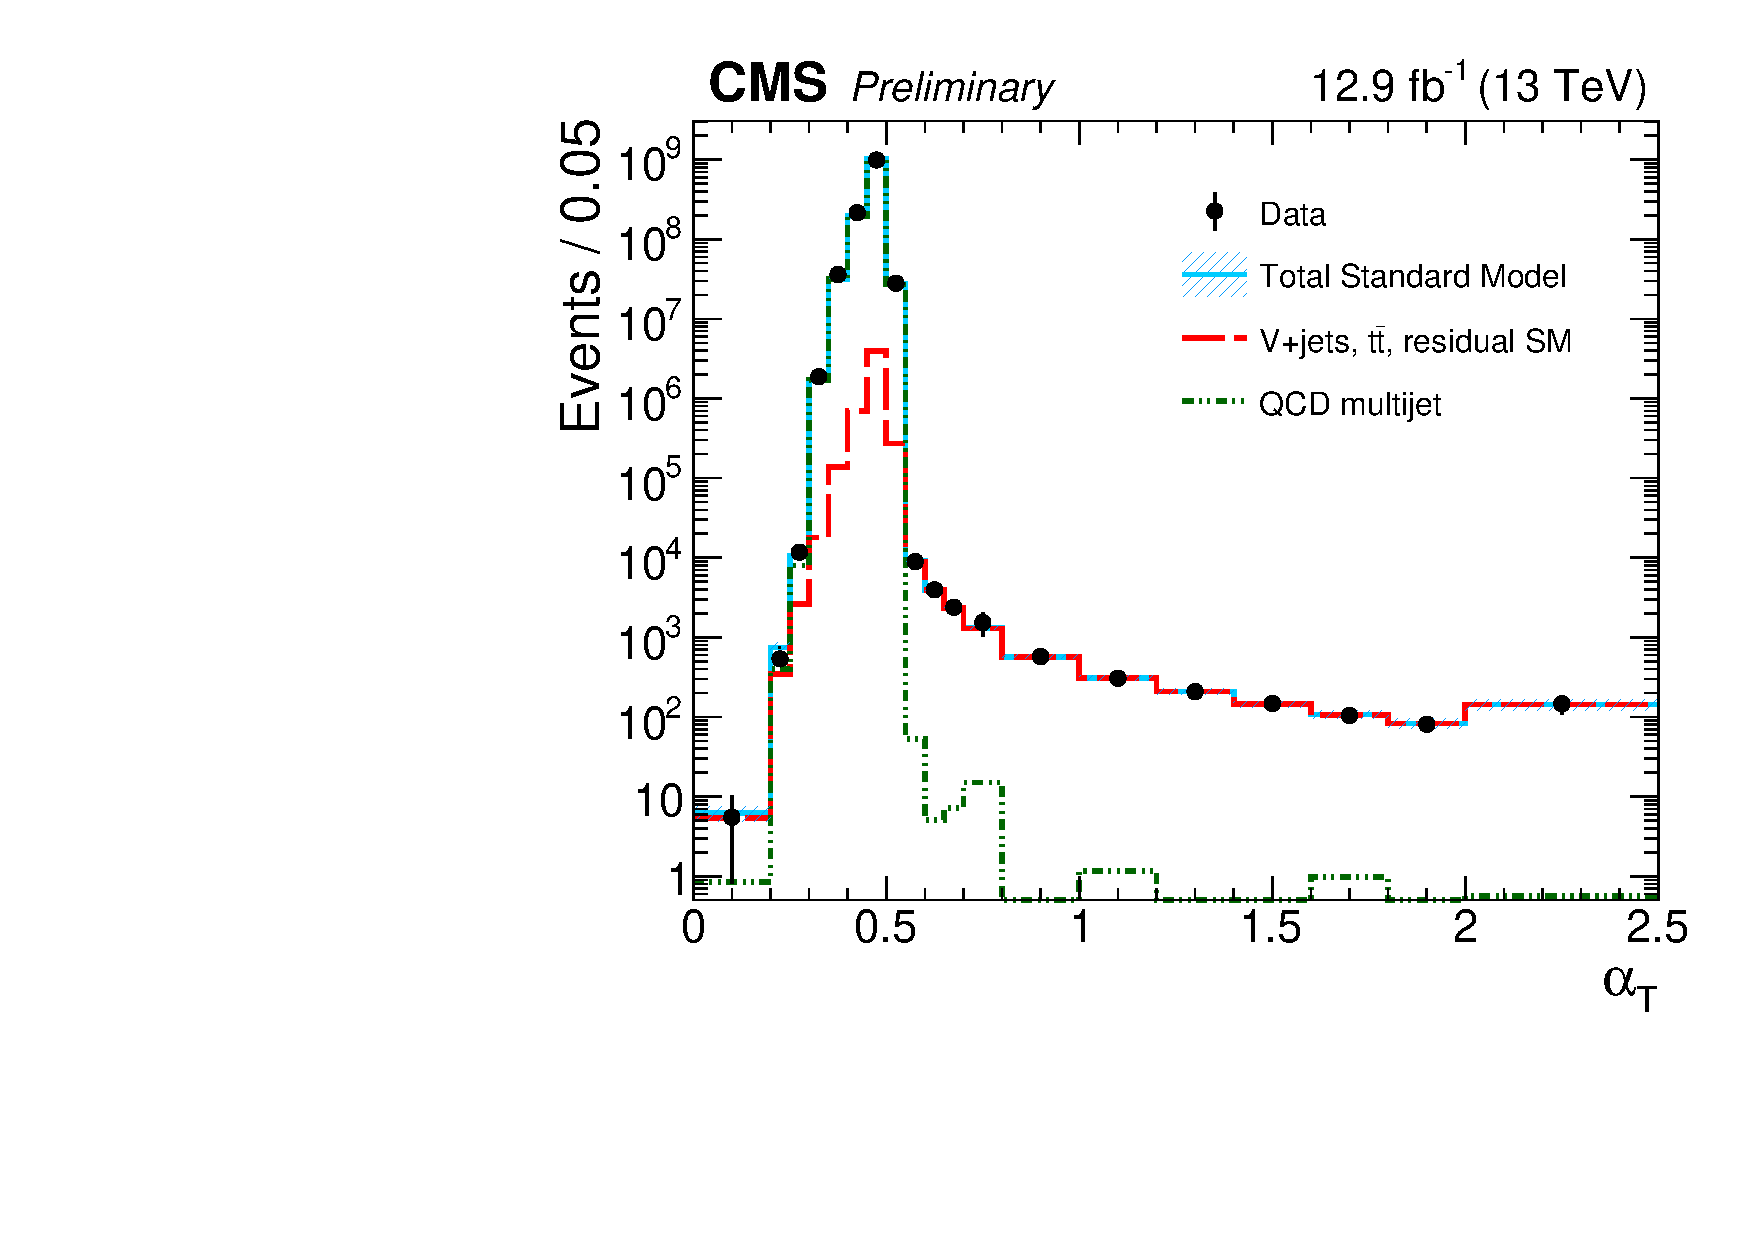
\includegraphics[width=0.5\textwidth]{figures/qcd/CMS-PAS-SUS-16-016_Figure-aux_001.pdf}
 }
 \subfigure[\dphimhtj distribution.\label{fig:bdphi_distr}]{
 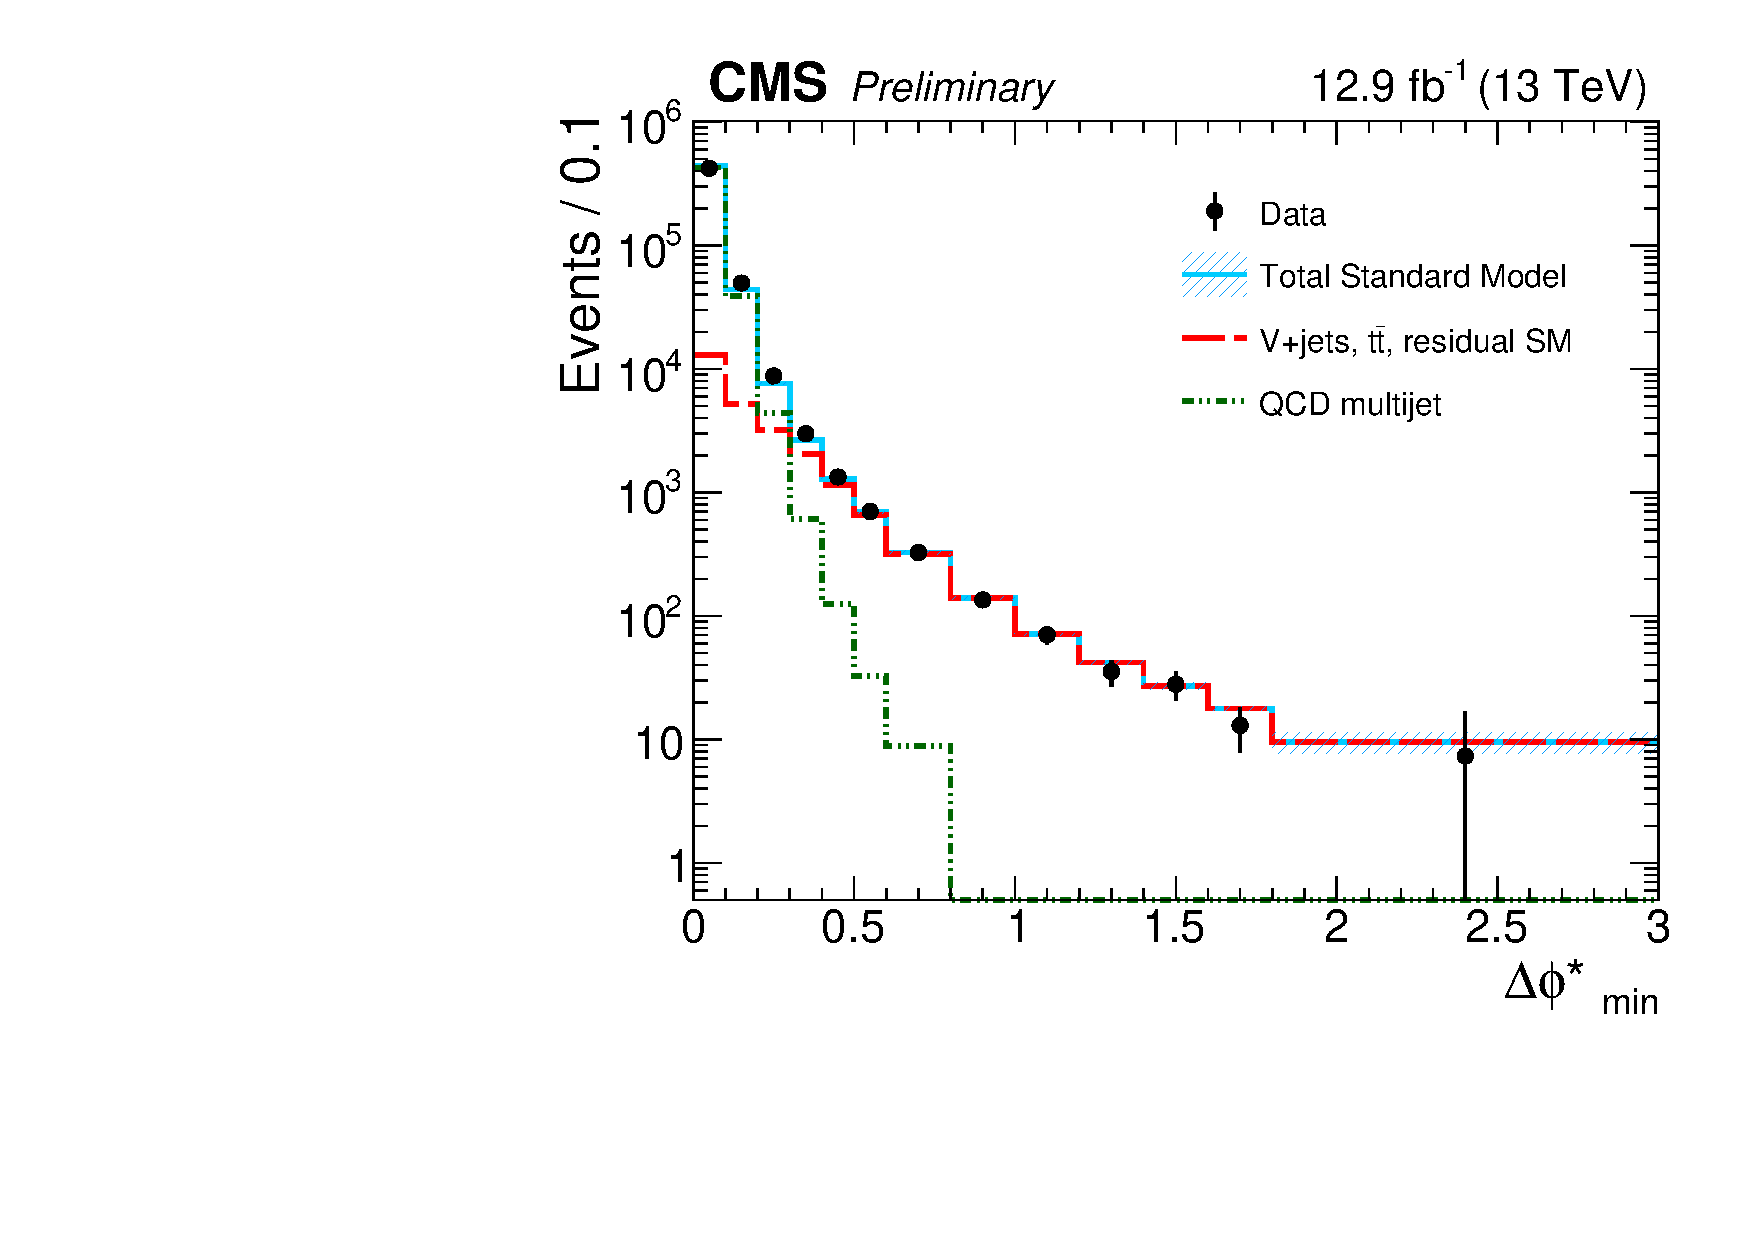
\includegraphics[width=0.5\textwidth]{figures/qcd/CMS-PAS-SUS-16-016_Figure-aux_002.pdf}
 } \\
 \caption{(Left) The \alphat distribution in data for events
   satisfying the pre-selection criteria when $\alphat < 0.55$ and the
   full signal selection criteria when $\alphat > 0.55$. (Right) The
   \bdphi distribution in data for events satisfying the pre-selection
   criteria and $\scalht > 800\GeV$. \fixme{Both plots need to be
     updated to the full data set.}  }
 \label{fig:alphat_bdphi_distr}
\end{figure}

\subsection{Overview of the method}
\label{sec:qcdMethod}

An estimate of the QCD multijet background is determined using three
multijet-enriched data sidebands, defined by inverting one or both
signal-region requirements on \bdphi and
$\mht/\met$. Table~\ref{tab:qcd_sidebands} summarises the requirements
for the three sideband regions and the signal region, labelled
\textbf{A}, \textbf{B}, \textbf{C}, and \textbf{D},
respectively. Further details on the selection requirements can be
found in Sec.~\ref{sec:multijetcontrolSelection}. The triggers used to
record the event samples are described in
Sec.~\ref{sec:control_samples}.

\begin{table}[h!]
  \caption{Definitions of data sidebands used in the determination of
    the QCD multijet background in the signal region. }  
  \label{tab:qcd_sidebands}
  \centering
  \footnotesize
  \begin{tabular}{ r|l|l }
                           & \multicolumn{1}{c|}{$0.2 < \bdphi < 0.5$} & \multicolumn{1}{c}{$\bdphi > 0.5$} \\[0.8ex]
    \hline
    $1.25 < \mhtmet < 3.0$ & \textbf{A} (``Double sideband'')         & \textbf{B} (``\mhtmet sideband'')  \\[0.8ex]
    \hline
    $\mhtmet < 1.25$       & \textbf{C} (``\bdphi sideband'')         & \textbf{D} (``Signal region'')     \\[0.8ex]
  \end{tabular}
\end{table}

The observed counts of events categorised according to \njet and
\scalht in each of the data sidebands are corrected to account for
contamination from nonmultijet SM processes. The corrected counts
$\mathcal{N}_i^\text{data}(\njet, \scalht)$ are assumed to arise
solely from QCD multijet production. The subscript $i$ indicates the
sideband under consideration (\textbf{A}, \textbf{B}, or
\textbf{C}). The nonmultijet processes, which comprise vector boson
and \ttbar production and residual contributions from other SM
processes, are estimated using the \mj control region, as described in
Section~\ref{sec:ewk_background}.

Independent ratios $\mathcal{R}_i^\mathrm{QCD}(\njet, \scalht)$ of the
number of multijet events that satisfy one or both of the
signal-region requirements to the number that fail the same
requirements are determined from simulation for events categorised
according to \njet and \scalht, and inclusively with respect to \nb
and \HTmiss. The subscript $i$ for each ratio $\mathcal{R}_i$
indicates the sideband (\textbf{A}, \textbf{B}, or \textbf{C}) from
which the extrapolation is being performed. The product of each ratio
$\mathcal{R}_i^\mathrm{QCD}(\njet, \scalht)$ and the corresponding
corrected data count $\mathcal{N}_i^\text{data}(\njet, \scalht)$
provides the estimate of the multijet background $\mathcal{P}_i(\njet,
\scalht)$. 

The estimates as a function of \njet, \scalht, \nb, and \HTmiss of the
signal region are assumed to factorise as follows:
\begin{equation}
  \label{eq:qcd1}
  \mathcal{P}_i( \njet, \scalht )  =
  \mathcal{N}_i^\text{data}( \njet, \scalht )\;
  \mathcal{R}_i^\mathrm{QCD}( \njet, \scalht ),
\end{equation}
\begin{equation}
  \label{eq:qcd2}
  \mathcal{P}_i( \njet, \scalht, \nb, \HTmiss ) = 
  \mathcal{P}_i( \njet, \scalht )\;
  \mathcal{K}_{\njet, \scalht}( \nb, \HTmiss ), 
\end{equation}
where the subscript $i$ refers to the sideband (\textbf{A},
\textbf{B}, or \textbf{C}). 

The $\mathcal{K}_{\njet, \scalht}( \nb, \HTmiss )$ are multiplier
terms that provide the estimated distribution of events as a function
of \nb and \HTmiss while preserving the normalisation $\mathcal{P}_i(
\njet, \scalht )$. Hence, the distribution of multijet events as a
function of \nb and \HTmiss, $\mathcal{K}_{\njet, \scalht}( \nb,
\HTmiss )$, is assumed to be identical to the distribution expected
for the nonmultijet backgrounds.

\subsection{Binned maximum-likelihood approach}
%estimate per \texorpdfstring{(\njet, \scalht)}{(Njet, HT)} bin}
% for \texorpdfstring{$\mathcal{P}_i( \njet, \scalht )$}{P(Njet,HT)}}

In this section, the multijet process is henceforth labelled as
``QCD''. The non-multijet processes (primarily \wj, \ttbar, and
\znunu) are henceforth labelled as collectively as the ``EWK''
processes.

A binned maximum-likelihood (ML) fit to data counts in each sideband,
analagous to that described in Sec.~\ref{sec:likelihood}, is performed
to obtain a estimate of the number of QCD multijet events in each
(\njet, \scalht) bin of a given sideband region. The EWK contributions
in the data sidebands are estimated using the ``transfer factor''
method, described in Sec.~\ref{sec:ewk-method}, and the \mj and \mmj
control regions, defined by the same selection criteria described in
Sec.~\ref{sec:control-region-selection} except for the inverted
requirement on the sideband variables. The fit to data assumes only
the presence of QCD and EWK contributions. Signal contamination is
expected to be negligible. All relevant systematic uncertainties in
the EWK background estimates are taken into account, including the
sources of experimental uncertainties described in Secs.~\ref{sec:}
and~\ref{sec:}. Independent fits are performed per sideband region.

The fit for each sideband region is used to constrain a free parameter
$\mu_{\textrm{QCD}}$ per (\njet, \scalht) bin that acts as a
multiplier term on the nominal QCD expection per bin, as determined
from simulation. The ML value of the (``signal strength'')
$\mu_{\textrm{QCD}}$ parameter per bin is applied to the nominal QCD
expectation (from simulation) in the corresponding bin of the signal
region to give an estimate for the QCD background. The three
independent fits therefore provide three independent predictions per
(\njet, \scalht) bin.

Figures~\ref{fig:mhtmet_sideband} (see Appendix~\ref{app:qcd})
summarises the following information obtained from the fit in the
$\mhtmet$ sideband: the observed data counts, the post-fit estimates
of the both the EWK and QCD contributions, and the constrained values
of the floating parameters $\mu_{\textrm{QCD}}$, as a function of
\njet and \scalht for the each of the sidebands. The pre-fit QCD
expectations are shown, but these can be inferred from the post-fit
expectations and ML values of $\mu_{\textrm{QCD}}$. Similarly, the
same information is shown for the \bdphi and ``double'' sidebands in
Figs~\ref{fig:bdphi_sideband} and~\ref{fig:double_sideband} (both in
Appendix~\ref{app:qcd}), respectively.

The QCD background estimate for each (\njet, \scalht) bin in the
signal region is determined from a weighted average of the predictions
based on each of the three sideband regions. 
%\footnote{In the case of zero QCD expectation in any given signal
%  region bin due to finite-size simulated event samples, the
%  uncertainty is estimated from neighouring bins.}
%the error is estimated by taking a poisson error with the average
%weight of QCD events in that bin before any analysis selection is
%applied.
%This takes advantage of the fact that different sidebands typically
%populate different ares of the \njet and \scalht phase space.  
Figure~\ref{fig:qcd_estimate} (Appendix~\ref{app:qcd}) shows the
(weighted) expected QCD background per (\njet, \scalht) bin, as
determined from the procedure above, and the expected EWK background
per bin in the signal region, as determined from the methods described
in Secs.~\ref{} and~\ref{}. Finally, the ratio of the QCD and EWK
background expectations per bin is also shown. The QCD background is
estimated to be negligible with respect to the EWK background,
typically below the percent level. This level of contamination is
compatible with the levels seen for pervious iterations of this
search, at both $\sqrt{s} = 8$ and 13\TeV. The predicted multijet
event counts are included as a background contribution to the
likelihood model, described in Sec~\ref{sec:likelihood}.

\subsection{Validation of the model and systematic uncertainties}
\label{sec:qcdValidation}

The reliance on simulation to model correctly the extrapolation from
each data sideband via the ratios $\mathcal{R}_i^\mathrm{QCD}$ is
validated by comparing the independent estimates $\mathcal{P}_i(\njet,
\scalht)$ from each sideband region. The level of closure in the
method is determed by comparing the differences in the ML values of
$\mu_{\textrm{QCD}}$ determined from each sideband region. The ML
values for $\mu_{\textrm{QCD}}$ determined from the \mhtmet and \bdphi
sideband regions are shown relative to the those obtained from the
``double'' sideband, the largest and purist event sample, in
Fig.~\ref{fig:qcdVal}. Bins for which there are insufficient event
counts in data or simulation to make the calculation are not
shown. Good agreement between the estimates indicates a good control
over the simulation modelling and the determination of EWK
contamination and trigger efficiencies in each of the sideband
regions. An adequate level of agreement between the independent
predictions is observed, and is amply covered by an assumed systematic
uncertainty of 100\% in each (weighted) estimate. This uncertainty is
assume to be unccorrelated across (\njet, \scalht) bins.

The distribution of multijet events as a function of \nb and \HTmiss,
$\mathcal{K}_{\njet, \scalht}( \nb, \HTmiss )$, is assumed to be
identical to the distribution expected for the nonmultijet
backgrounds. This final assumption is based on studies in simulation
and is a valid approximation given the magnitude of this background
contribution, as well as the magnitude of the statistical and
systematic uncertainties in the ratios
$\mathcal{R}^\mathrm{QCD}(\njet, \scalht)$, as described above.

%As the prediction of QCD in the signal region is carried out
%inclusively over \nb and \mht, the QCD shapes for these variables are
%taken from the EWK simulation and normalised to the QCD counts.  A
%lack of statistics in the QCD MC led to the adoption of this approach.
% To validate it, the simulated \mht distributions
% for the QCD and EWK processes in the signal region are divided. This is shown in
% Figs.~\ref{fig:qcd_validation}.%~\ref{fig:asym_qcd_validation}-\ref{fig:asym_qcd_validation}.
% As the normalisation is carried out independently, a flat distribution
% of the ratio is enough for validation. Within uncertainties, the level of agreement is acceptable given the
% small total QCD contribution to the signal region and its large
% systematic uncertainty.






%%____________________________________________________________________________||

\section{``Lost lepton'' background estimation}
\label{sec:ttw}

Once all the signal region selection requirements have been imposed,
the contribution from QCD multijet events is expected to be
negligible, as demonstrated in Sec.~\ref{sec:qcd}. In the absence of
multijet events, the background counts in the signal region arise from
SM processes with significant \met in the final state. In events with
low counts of jets and b-quark jets, the largest backgrounds with
genuine \met are from the associated production of W or Z bosons with
jets, followed by either the weak decays \znunu or \wtaunu, where the
$\tau$ decays hadronically and is identified as a jet; or by leptonic
decays that are not rejected by the dedicated electron or muon
vetoes. The veto of events containing isolated tracks is efficient at
further suppressing these backgrounds as well as the single-prong
hadronic decay of the tau lepton. At higher jet and b-quark jet
multiplicities, top quark production followed by semileptonic weak top
quark decay becomes important.  Residual contributions from processes
such as single-top-quark, $\ttbar$V or $\ttbar$H, diboson, and
Drell-Yan production are also expected. These SM processes are
collectively referred to as the non-multijet backgrounds. 

The ``lost lepton'' background consists primarily of processes
yielding at least one W boson, which decays leptonically and the
result lepton is either outside the experimental acceptance or does
not satisfy requirements related to reconstruction ``quality'' or
isolation. Predominantly, the lost lepton background arises from the
\wj and \ttbar processes, which smaller contributions from processes
such as single top, {\ttbar}V, {\ttbar}H, \etc All these processes,
plus any others that yield non-negligible contributions are estimated
using the \mj control region. (The \mmj sample is reserved to estimate
solely the \znunu\ background.)

\subsection{The ``transfer factor'' method}
\label{sec:tf-method-ttw}

The method used to estimate the lost lepton background relies on the
use of a transfer factor (TF) determined from simulated event samples
to transform the observed event yields in the \mj sample, categorised
according to \njet, \scalht, and \nb, $\nobs^{\mj}(\njet, \scalht,
\nb)$, into an estimate of the lost lepton background for the
corresponding (\njet, \scalht, \nb) category of the signal region,
$\npre^{\ttw}(\njet, \scalht, \nb)$. The categorisation of events
according to \njet, \scalht, and \nb in the \mj control region is
identical to that for the signal region, as defined in
Sec.~\ref{sec:selection}.\footnote{One detail here is that predictions
  are made according to the \scalht categorisation used in the control
  regions (up to 11 bins), but the predictions are then aggregated
  over a range in \scalht to map onto a coarser binning scheme is used
  in the signal region (up to 5 bins). Further details can be found in
  Sec.~\ref{sec:ht-categorisation}.}  Each transfer factor is simply a
ratio of the yields obtained from Monte Carlo (MC) simulation for the
same (\njet, \scalht, \nb) category of the \mj control and signal
regions:
\begin{equation}
  \label{equ:tf-ratio}
  {\rm TF} = \frac{N_{\rm MC}^{\ttw}(\njet, \scalht, \nb)}{N_{\rm MC}^{\mj}(\njet, \scalht, \nb)} 
\end{equation}

In this way, predictions for the lost lepton background can be made,
based on the \mj control region, as follows:
\begin{equation}
  \label{equ:pred-method}
  \npre^{\ttw}(\njet, \scalht, \nb) = 
  \frac{N_{\rm MC}^{\ttw}(\njet, \scalht, \nb)}{N_{\rm MC}^{\mj}(\njet, \scalht, \nb)} 
  \times 
  \nobs^{\mj}(\njet, \scalht, \nb)   
\end{equation}

The selection criteria for the \mj control region
(Sec.~\ref{sec:selection}) closely resemble those for the signal
region, differing mainly through the use of a muon {\it tag} (that is
ignored in the calculation of jet-based kinematic variables such as
\scalht, \mht, \alphat, \etc) and minimal additional kinematic
requirements (\eg a transverse mass window) to obtain a sample
enriched in \wj and \ttbar events. The same selection criteria are
designed to suppress signal contamination so that unbiased data-driven
estimates for the SM backgrounds in the signal region can be
made. Any signal contamination is accounted for in the likelihood
model (Sec.~\ref{sec:likelihood}). 

Figure~\ref{fig:tf_muToTtw} (App.~\ref{app:ttw}) shows the magnitude
of the transfer factors, typically $\ll 1$, The transfer factors
account for differences between the \mj control and signal due to the
acceptance times efficiency for the reconstructed muon and
extrapolations in kinematic quantities. For example, the dependence on
\njet, \scalht, and \nb is largely attributable to the \alphat and
\bdphi requirements for the signal region (that are not used in the
\mj control region).

Many systematic effects are expected to cancel largely in the transfer
factor. However, a systematic uncertainty is assigned to each transfer
factor to account for theoretical uncertainties and effects such as
the mismodelling of kinematics (\eg acceptances) and instrumental
effects (\eg reconstruction efficiencies). These uncertainties are
discussed below. 

\subsection{\texorpdfstring{\mht}{MHT} templates}

The transfer factors described above provide an estimate of the lost
lepton background as a function of the (\njet, \scalht, \nb) category,
but inclusive with respect to \mht. However, the analysis utilises the
\mht variable to discriminate effectively between SM background and
\eg a potential contribution from SUSY processes. The \HTmiss
information is incorporated into the likelihood model via an \mht
template per (\njet, \scalht, \nb) category, $N_{\rm
  MC}^{\ttw}(\HTmiss;\; \njet, \scalht, \nb)$, which is equivalent to
dicing the numerator of the TF according to \mht, \ie
\begin{equation}
  \label{equ:pred-method-mht}
  \npre^{\ttw}(\njet, \scalht, \nb, \HTmiss) = 
  \frac{N_{\rm MC}^{\ttw}(\HTmiss;\; \njet, \scalht, \nb)}{N_{\rm MC}^{\mj}(\njet, \scalht, \nb)} 
  \times 
  \nobs^{\mj}(\njet, \scalht, \nb)
\end{equation}
In this regard, the TFs described in Sec.~\ref{sec:tf-method-ttw}
provide an estimate of the normalisation for each \mht template. The
\HTmiss templates are taken from simulation and the validity of the
simulation modelling is tested extensively in the control regions, as
described in Sec.~\ref{sec:mht}. 

\subsection{Sideband normalisation for \texorpdfstring{\wj}{W+jets} and \texorpdfstring{\ttbar}{TTbar}} 
\label{sec:sideband-corrections}

In this section, a procedure is described to derive process-dependent
``sideband corrections'' by means of a binned likelihood fit using
data sidebands to the \mj and \mmj control regions. Various different
data sidebands have been considered. However, the one used in this
procedure is the \HTmiss sideband, defined by $100 < \HTmiss <
200\GeV$.

Corrections to the inclusive cross sections of the dominant processes
in the signal and control regions, namely \wj and \ttbar, as well as
\zmmj and \znunuj, are determined.\footnote{Corrections for the latter
  two processes, \zmmj and \znunuj, are discussed in further \ detail
  in Sec.~\ref{sec:sideband-corrections-zinv}.} These corrections are
derived after all relevant corrections are applied to the simulated
samples. Hence, these corrections are expected to be near unity for
each process given that, for example, the simulated samples are
normalised to the integrated luminosity of the data sets using the
most accurate cross section calculations available, typically NNLO or
better. However, there are various potential sources of bias that may
lead to a non-negligible correction. For example, non-unity
corrections may be due to the limited applicability of inclusive cross
section calculations in the high-\scalht, high-\ETmiss corner of phase
space used in this analysis.

It is important to note that this iteration of the analysis is {\em
  not} sensitive to whether these corrections are applied or not, due
to the way the transfer factors are constructed. The \mj sample, rich
in \wj and \ttbar events, is used to predict the lost lepton
background. Both control regions are constructed and binned to cover a
kinematically similar phase space. Hence, the extrapolations are
minimal and so the corrections have little impact on the transfer
factors.

However, the corrections are still determined and propagated to all
steps of the analysis, as they are relevant for some of the
data-driven derivation of systematic uncertainties, such as the
closure tests (Sec.~\ref{sec:closure-tests}) and cross checks of the
\HTmiss modelling (Sec.~\ref{sec:mht}). Without these corrections, the
derived systematic uncertainties could be (unnecessarily)
inflated. Further, the uncertainty in these corrections are not
propagated, as any inaccuracy is -- by construction -- covered by the
aforementioned data-driven procedures to determine systematic
uncertainties.

The \HTmiss sidebands to the control regions are defined with an
identical acceptance to the control regions (except for the \HTmiss
requirement itself) and the sidebands are binned identically in terms
of \njet, \scalht, and \nb. 

A single floating parameter per dominant process, namely \wj, \ttbar,
and \zllj, encodes the correction for that process (fully correlated
across all bins).  The \wj and \ttbar processes are constrained by the
\mj sideband.\footnote{The \zllj process is constrained by the \mmj
  sideband. The correction derived for \zllj is also applied to the
  \znunu + jets simulated event sample. Details can be found in
  Sec.\ref{sec:sideband-corrections-zinv}.}  The corrections and
uncertainties for \wj and \ttbar, as determined by the fit, are shown
in Table~\ref{tab:sbCorrsFromFit}.

\begin{table}[!h]
  \scriptsize
  \centering
  \topcaption{Corrections to the inclusive cross sections 
    for SM processes determined from a binned likelihood fit to data
    in the $100 < \HTmiss < 200\GeV$ sideband to the control regions.}  
  \label{tab:sbCorrsFromFit}
  \begin{tabular}
    {clc}
    \hline
    \textbf{Process} & \textbf{Sample} & \textbf{Corrrection} \\
    \hline
%    \wj              & \mj             & $1.21 \pm 0.01$      \\ % no NLO/NISR 
%    \ttbar           & \mj, \mmj       & $0.92 \pm 0.01$      \\ % no NLO/NISR
    \wj              & \mj             & $1.06 \pm 0.01$      \\
    \ttbar           & \mj, \mmj       & $0.93 \pm 0.01$      \\
    \hline
  \end{tabular}
\end{table}

\subsection{Overview of systematic uncertainties}
\label{sec:systematics}

The following sections address the estimation of systematic
uncertainties related to the lost lepton background estimation. All
relevant uncertainties are listed in Table~\ref{tab:systs-ttw}, along with
their representative magnitudes and assumptions on inter-bin
correlations. How the uncertainties are incorporated into the
likelihood model is described in Sec.~\ref{sec:likelihood}. 

\begin{table}[h!]
  \caption{Sources of systematic uncertainty in the transfer factors
    used to estimate the lost lepton background using the \mj control
    region. Also shown are the nuisance parameters and correlation
    scheme, as well as representative magnitudes for the uncertainties
    [\%]. The ``type'' refers to whether the nuisance parameters are
    unique to the lost lepton background or shared with the \znunuj
    background estimate (see Table~\ref{tab:systs-zinv}). 
  }   
  \label{tab:systs-ttw}
  \centering
  \fontsize{8}{9.6}\selectfont
  \begin{tabular}{ llllc }
    \hline
    Source of uncertainty               & Nuisance parameters / correlation              & Magnitude (\%)               & Type   & Figure                              \\
    \hline
    Finite-size simulated samples       & 1 per (\njet, \scalht, \nb, \mht) categories   & 1--100                       & Unique & n/a                                 \\
    Minimum bias cross section (pileup) & 1, correlated across \njet, \scalht, \nb, \mht & X--Y                         & Shared & \ref{fig:tfSyst_pu_muToTtw}         \\
    $\mu_R$ / $\mu_F$ scales            & 1, correlated across \njet, \scalht, \nb, \mht & X--Y                         & Shared & \ref{fig:tfSyst_scale_muToTtw}      \\
    Parton density functions            & 1, correlated across \njet, \scalht, \nb, \mht & X--Y                         & Shared & \ref{fig:tfSyst_pdf_muToTtw}        \\
    \wj cross section                   & 1, correlated across \njet, \scalht, \nb, \mht & 0.0--1.4                     & Unique & \ref{fig:tfSyst_wjetxs_muToTtw}     \\
    \ttbar cross section                & 1, correlated across \njet, \scalht, \nb, \mht & 0.0--1.7                     & Unique & \ref{fig:tfSyst_ttbarxs_muToTtw}    \\
    QCD + EWK NLO corrections           & 1, correlated across \njet, \scalht, \nb, \mht & 0.2--10.2                    & Shared & \ref{fig:tfSyst_nlo_muToTtw}        \\
    $N_\textrm{isr}$ (\ttbar)           & 1, correlated across \njet, \scalht, \nb, \mht & 0.0--8.8                     & Unique & \ref{fig:tfSyst_nisr_muToTtw}       \\
    Signal trigger efficiency           & 1, correlated across \njet, \scalht, \nb, \mht & 0.0--3.1                     & Shared & \ref{fig:tfSyst_trigger_muToTtw}    \\
    Lepton efficiency (selection)       & 1, correlated across \njet, \scalht, \nb, \mht & 0.0--4.2                     & Unique & \ref{fig:tfSyst_muonsf_muToTtw}     \\
    Lepton efficiency (veto)            & 1, correlated across \njet, \scalht, \nb, \mht & X--Y                         & Unique & \ref{fig:tfSyst_leptonveto_muToTtw} \\
    Jet energy scale                    & 1, correlated across \njet, \scalht, \nb, \mht & 3.3--7.0                     & Shared & \ref{fig:tfSyst_jec_muToTtw}        \\
    b-quark tag efficiency              & 1, correlated across \njet, \scalht, \nb, \mht & 0.3--0.6                     & Shared & \ref{fig:tfSyst_bsf_muToTtw}        \\
    b-quark mistag probability          & 1, correlated across \njet, \scalht, \nb, \mht & 0.1--1.7                     & Shared & \ref{fig:tfSyst_bsfl_muToTtw}       \\
    \alphat + \bdphi extrapolation      & 1 per \njet category, 1 per \scalht category   & X--Y (\njet), X--Y (\scalht) & Unique & \ref{fig:closure_AlphaT_bDPhi_mu}   \\
%    \alphat extrapolation              & 1 per \njet category, 1 per \scalht category   & X--Y (\njet), X--Y (\scalht) & Unique & \ref{fig:closure_AlphaT_mu}         \\
%    \bdphi extrapolation               & 1 per \njet category, 1 per \scalht category   & X--Y (\njet), X--Y (\scalht) & Unique & \ref{fig:closure_bDPhi_mu}          \\
    W polarisation                      & 1 per \njet category, 1 per \scalht category   & X--Y (\njet), X--Y (\scalht) & Unique & \ref{fig:closure_WPol_mu}           \\
    Single isolated track veto          & 1 per \njet category, 1 per \scalht category   & X--Y (\njet), X--Y (\scalht) & Unique & \ref{fig:closure_SITV_mu}           \\
    \hline
  \end{tabular}
\end{table}

Several sources of uncertainty are evaluated.  The most relevant
effects are discussed below, and generally fall into one of two
categories. The first category concerns known theoretical and
experimental effects that are propagated through to the transfer
factors and \HTmiss templates. These are decribed in
Sec.~\ref{sec:mc-variations}. The second set can be considered as
``known unknowns'' that are derived from dedicated ``closure test''
and \HTmiss-modelling studies that involve confronting transfer
factors determined in the phase space of this search against data in
the control regions. This latter category of uncertainties are
summarised in Secs.~\ref{sec:closure-tests} and
\ref{sec:mht}.

%These uncertainties will be often referred to as
%\textit{``normalisation uncertainties''}, as opposed to the
%\textit{``\HTmiss template uncertainties''} described in
%Sec.~\ref{sec:syst-on-shape}. The former affect the total number of
%events in each (\njet,~\nb,~\scalht) bin (integrating over \mht),
%while the latter encode the limited knowledge on how these events
%distribute in the \mht dimension. The two sets of systematic
%uncertainties have a separate treatment.

\subsection{Known theoretical and experimental uncertainties}
\label{sec:mc-variations}

A set of corrections are applied to the simulated samples in order to
account for known theoretical and experimental biases, such as jet
energy response, b-tagging efficiency, \etc These corrections are
described in Sec.~\ref{sec:sim-corrs}. These corrections are provided
with uncertainties to cover assumptions in the procedures used in
their derivation. Further sources of uncertainties are also
considered, such as the use of LO generators. The effect of various
uncertainties on the transfer factors and \HTmiss templates is
discussed below.

These sources of uncertainty are each assumed to originate from a
unique underlying source and so the effect of each source is varied
assuming a fully correlated behaviour across the full phase space of
the signal and control regions.

\subsubsection{Minimum bias cross section / pileup}
\label{sec:tfSyst_pu}

Events in simulation are reweighted in order to match the distribution
of the primary vertex multiplicity observed in data
(Sec.~\ref{sec:pileup-reweighting}).  A systematic uncertainty is
derived by propagating the 5\% uncertainty on the minimum bias cross
section used in the reweighting procedure.  The relative change in the
transfer factors under this variation is small, at the few percent
level, as shown in Fig.~\ref{fig:tfSyst_pu_muToTtw}
(App~\ref{app:ttw}).

\subsubsection{Effect of scale and PDF on lepton acceptance}
\label{sec:tfSyst_pdf}

Theoretical uncertainties from choices in the renormalisation and
factorisation scales, as well as the parton distribution function, can
introduce systematic uncertaintes on lepton acceptance. The scales
$\mu_R$ and $\mu_F$ are varied by 0.5 and 2.0. Theoretical
uncertainties from parton distribution function are varied according
to the recommended prescription from PDF4LHC~\cite{PDF4LHC:2015}. The
magnitude of the variations in the transfer factors are small,
typically at the $\sim X\%$
level. Figures~\ref{fig:tfSyst_scale_muToTtw} and
\ref{fig:tfSyst_pdf_muToTtw} (App.~\ref{app:ttw}) show the behaviour
in the transfer factors for variations in scale and PDF, respectively.

\subsubsection{\texorpdfstring{\wj}{W+jets} and \texorpdfstring{\ttbar}{TTbar} composition}
\label{sec:tfSyst_ttW_composition}

The relative composition of \wj with respect to \ttbar in the \mj
control region differs relative to that in the signal region, due to
the application of different kinematic requirements (\eg \mt in the
control region, \alphat and \bdphi in the signal region). Hence,
uncertainties in the inclusive cross sections for \wj and \ttbar may
result in variations in the transfer factors as a function of \njet,
\scalht, and \nb, as well as the \HTmiss templates.

A correction to the inclusive cross sections is applied via the
procedure described in Sec.~\ref{sec:sideband-corrections}, which
adjusts the normalisation of the simulated \wj and \ttbar event
samples to match the data counts in a \HTmiss sideband that
(otherwise) covers an identical region of phase space to the \mj
control region.

Following this procedure, the normalisation for the \wj process is
varied by twice the relative uncertainty in the latest CMS measurement
of the inclusive cross section, while preserving the {\it sum} of the
\wj and \ttbar (and other residual) contributions integrated across
the full phase space of the signal region and, separately, the \mj
control region, in order to see the effect on the ``shape'' of the
transfer factors and the \HTmiss templates. Similarly, the same same
procedure is repeated for variations in the \ttbar normalisation. The
resulting variations are summarised in
Fig.~\ref{fig:tfSyst_ttW_composition_muToTtw} (App.~\ref{app:ttw}).

\subsubsection{Missing higher-order corrections in LO \texorpdfstring{\MADGRAPH}{MadGraph}
  samples}
\label{sec:nlo}

The \wj process are generated at leading order with the \MADGRAPH
code. The effect of missing higher-order QCD and EWK corrections are
studied by considering the effect of LO$\rightarrow$NLO corrections,
determined as a function of W boson \Pt and shown in in
Fig.~\ref{fig:tfSyst_nlo_muToTtw} (App.~\ref{app:ttw}), on the
transfer factors and \HTmiss templates. 

Simulated \wj events are weighted according to these NLO corrections,
and the magnitude of each correction is propagated as an uncertainty
throughout the analysis. Fig.~\ref{fig:tfSyst_nlo_muToTtw}
(App.~\ref{app:ttw}) show the effect on the transfer factors as a
function of the various discriminating variables. Uncertainties are
typically at the percent level and as large as $\sim 10\%$.

%All events in the control and signal regions are categorised
%identically according to \njet and \scalht. The NLO corrections are
%determined based on matrix element calculations that consider up to 3
%(1) radiated partons for QCD (EWK) processes. Hence the calculations
%are not necessarily correct for the high-\njet phase space covered by
%this analysis. Hence, these NLO corrections are not applied directly,
%but instead are propagated as an uncertainty through the
%analysis. Fig.~\ref{fig:tfSyst_nlo_muToTtw} (App.~\ref{app:ttw}) show
%the effect on the transfer factors as a function of the various
%discriminating variables. Uncertainties are typically at the percent
%level and as large as $\sim 10\%$.

\subsubsection{\texorpdfstring{\njet}{Njet}-dependent (``\texorpdfstring{\nisr}{Nisr}'') corrections for \texorpdfstring{\ttbar}{TTbar}}
\label{sec:nisr}

The recommendations from the SUSY group to reweight \MADGRAPH \ttbar
Monte Carlo events according to the number of ISR jets ($N_J^{ISR}$)
identified in the event is described in
Sec.~\ref{sec:nisr}. 

All events in the control and signal regions are categorised
identically according to \njet, hence the analysis is not sensitive to
the $N_\textrm{isr}$ corrections. Regardless, these corrections are
applied to simulated \ttbar event, and half the correction is
propagated as an uncertainty throughout the
analysis. Fig.~\ref{fig:tfSyst_nisr_muToTtw} (App.~\ref{app:ttw}) show
the effect on the transfer factors as a function of the various
discriminating variables. Uncertainties are in typically $\ll 5\%$.

\subsubsection{Signal trigger uncertainty}
\label{sec:tfSyst_trigger}

The effect of uncertainties in the signal trigger efficiency for the
signal region are studied (Sec.~\ref{sec:triggers}). A systematic is
taken as the difference in the efficiency measured using muon and
electron reference triggers.  The relative change in the transfer
factors is typically at the few percent level, as presented in
Fig.~\ref{fig:tfSyst_trigger_muToTtw} (App~\ref{app:ttw}).

\subsubsection{Lepton trigger / identification / isolation efficiencies}
\label{sec:leptonSyst}

The number of events $N^{\mj}$ in the \mj control region is given by
\begin{equation}
  \label{eq:lepton_eff_mj}
  N^{\mj} = 
  N^\textrm{gen}_\mu \,
  \mathcal{A}_\mu \,
  \varepsilon^\textrm{trig}_\mu \,
  \varepsilon^\textrm{ID}_\mu \,
  \varepsilon^\textrm{iso}_\mu  
\end{equation}
where: $N^\textrm{gen}_\mu$ is the expected number of simulated events
(weighted to the integrated luminosity) containing a generator-level
prompt muon prior to event selection requirements; and
$\mathcal{A}_\mu$, $\varepsilon^\textrm{trig}_\mu$,
$\mathcal{A}_\mu$, $\varepsilon^\textrm{ID}_\mu$, and
$\varepsilon^\textrm{iso}_\mu$, are the muon acceptance and the
trigger, identification, and isolation efficiencies, respectively,
which are assumed to factorise. 

%The number of events $N^\textrm{SR}$ in the signal region is defined
%by
%\begin{equation}
%  \label{eq:lepton_eff_sr}
%  N^\textrm{SR} 
%  \; = \; 
%  \sum_{\ell = \mu,e} \; N^\textrm{SR}_\ell
%\end{equation}
%where $N^\textrm{SR}_\ell$ is the number of events containing a
%generator-level particle $\ell$ in the signal region, and the
%summation is performed assuming $\ell$ is either a generator-level
%prompt muon or electron.

The number of events $N^\textrm{SR}$ in the signal region is given by
\begin{equation}
  \label{eq:lepton_eff_sr}
  N^\textrm{SR} 
  \; = \; 
  \sum_{\ell = \mu,e} 
  N^\textrm{gen}_\ell 
  \; [ \;
  (1-\mathcal{A}_\ell)
  \; + \;
  \mathcal{A}_\ell \,
  (1-\varepsilon^\textrm{trig}_\ell)
  \; + \;
  \mathcal{A}_\ell \,
  \varepsilon^\textrm{trig}_\ell \,
  (1-\varepsilon^\textrm{ID}_\ell)
  \; + \;
  \mathcal{A}_\ell \,
  \varepsilon^\textrm{trig}_\ell \,
  \varepsilon^\textrm{ID}_\ell \,
  (1-\varepsilon^\textrm{iso}_\ell)
  \; ]
\end{equation}
where: $N^\textrm{gen}_\ell$ is the expected number of simulated
events (weighted to the integrated luminosity) containing the
generator-level particle $i$ prior to event selection requirements;
and $\mathcal{A}_\ell$, $\varepsilon^\textrm{ID}_\ell$, and
$\varepsilon^\textrm{iso}_\ell$ are the experimental acceptance and
the trigger, identification, and isolation efficiencies for the lepton
$\ell$, respectively. The summation is performed assuming $\ell$ is
either a generator-level prompt muon or electron. The four terms of
Eq.~\ref{eq:lepton_eff_sr} are assumed to factorise and provide
the number of events (containing either a muon or an electron) that
fail requirements on acceptance, trigger, identification, and
isolation, respectively.

The effect of theory related uncertainties on lepton acceptance,
$\mathcal{A}_\ell$, for the \mj control and signal regions is
described in other sections (\eg Sec.~\ref{sec:tfSyst_pdf} for scale
and PDF uncertainties).

The effect of experimental uncertainties in efficiency measurements
related to trigger, identification, and isolation requirements are
dsecribed below for both the \mj sample (Eq.~\ref{eq:lepton_eff_mj})
and signal region (Eq.~\ref{eq:lepton_eff_sr}).

\subsubsection*{Selection efficiencies (\texorpdfstring{\mj}{mu+jets} control region)}

The various efficiencies in Eq.~\ref{eq:lepton_eff_mj} are emulated as
part of the detector simulation. Further, (typically near-unity)
data/simulation scale factors are determined and applied to the
simulated events to ensure the emulated efficiencies match the
corresponding measurements in data.

The muon trigger efficiency $\varepsilon^\textrm{trigger}_\mu$ is
emulated in the simulation. Data/MC scale factors provided by the muon
POG are applied to account for differences in the determination of the
muon trigger efficiency from data and simulation. The scale factors
are near-unity and their uncertainties are at the percent level. 

The Tight working point for identification and relative isolation
requirements are applied, as described in
Sec.~\ref{sec:muon-id}. Data/simulation scale factors provided by the
muon POG are applied. Again, the scale factors are near-unity and
their uncertainties are at the percent level.

Finally, $\eta$-dependent muon tracking scale factors provided by the
muon POG, to cover inefficiencies due to the ``HIP effect'', have been
applied and their uncertainties taken into consideration. Their effect
is typically at the percent level. 

The uncertainties in the scale factors have been propagated through to
the transfer factors and \mht templates. A flat 2\% uncertainty, shown
in Fig~\ref{fig:tfSyst_muonsf_muToTtw} (App.~\ref{app:ttw}), fully
correlated in \njet, \scalht, \nb, and \mht, is assumed to cover the
aforementioned effects.

\subsubsection*{Veto efficiencies (signal region)}

Uncertainties in the signal trigger efficiencies are covered in
Sec.~\ref{sec:tfSyst_trigger}. In terms of vetoing leptons (both muons
and electrons) within the experimental acceptance of the signal
region, the Loose working point for identification and
``mini-isolation'' requirements are applied, as detailed in
Secs.~\ref{sec:muon-id} and \ref{sec:electron-id}. The data/simulation
scale factors are provided by the SUSY scale factor working
group~\cite{twiki-leptonSF}. Again, the scale factors are near unity
with uncertainties of a few percent, which have been propagated
through to the transfer factors and \mht templates. A flat 5\%
uncertainty, shown in Fig~\ref{fig:tfSyst_leptonveto_muToTtw}
(App.~\ref{app:ttw}), fully correlated in \njet, \scalht, \nb, and
\mht, is assumed to cover the aforementioned effects. This uncertainty
is assumed to be anti-correlated with respect to the corresponding
uncertainty in the \mj control region, described above. 

\subsubsection{Jet energy scale}
\label{sec:tfSyst_jec}

The effect of varying the jet energy scale in the \mj and \mmj control
regions is investigated.  The energies of jets used in the analysis
are corrected as a function of their \pt and $\eta$ via the procedure
recommended by the JetMET POG. These corrections have an associated
uncertainty, which is propagated through the analysis.  As the \scalht
and jet multiplicity binning is mirrored in signal and control
regions, the effect of jet energy scale on the transfer factor is
expected to be small.  However, the jet energy scale can still have an
effect due to jets moving in and out acceptance (above and below
$40\gev$). The relative change in the transfer factors is presented as
a function of \scalht and jet category in
Fig.~\ref{fig:tfSyst_jec_muToTtw} (App.~\ref{app:ttw}). The changes
are typically in the range of $1-5\%$.

\subsubsection{B-tagging efficiency and mistag probability}
\label{sec:tfSyst_btag}

Scale factors provided by the BTV POG are applied to the MC samples to
correct for differences in the b-tagging efficiencies and
misidentifications between simulation and data.  The method employed
is based on simple event reweighting as described in
Ref.~\cite{btagSFMethods}.  Events are reweighted according to the
probability of obtaining a particular jet configuration in data and
simulation, as determined by the b-tagging efficiencies computed in
the MC samples and the scale factors measured in data.  Since no
extrapolation is performed in the background prediction across
different \nb multiplicities, the analysis is expected to be robust
against variations in the b-tagging efficiency.  To test this effect
the change in the transfer factors is measured by varying the scale
factors within their uncertainties. The scale factors associated with
b and c jets are varied together (since their measurements are
correlated), while those associated with light jets are varied
separately.  The relative change in the transfer factors is presented
as a function of \scalht and jet category in
Figs.~\ref{fig:tfSyst_bsf_muToTtw} and \ref{fig:tfSyst_bsfl_muToTtw}
(App.~\ref{app:ttw}).  They are typically in the range of $1-3\%$.

\subsection{Systematics uncertainties from data-driven tests}
\label{sec:closure-tests}

The second category of uncertainty is determined from sets of closure
tests based on data control samples~\cite{RA1Paper2012}.  Each set of
tests targets a specific (potential) source of bias in the simulation
modelling that may introduce an \njet- or \scalht-dependent source of
systematic bias in the transfer factors~\cite{RA1Paper2012}.

The level of closure with respect to data is inspected:
\begin{itemize}
\item as a function of \njet while integrating over \scalht and \nb; 
\item as a function of \scalht while integrating over \njet and \nb;
\item as a function of \nb, while integrating over \njet and \scalht.
\end{itemize}
Any non-closure is covered by a systematic uncertainty based on
summing in quadrature the level of closure and its statistical
uncertainty. The magnitude of the uncertainties are summarised in
Table~\ref{tab:systs-ttw} in Sec.~\ref{sec:systematics}. In the
likelihood model (Sec.~\ref{sec:likelihood}), one log-normal nuisance
parameter is used per \scalht category (\ie correlated over \njet and
\nb) and per \njet category (\ie correlated over \scalht and \nb) for
all sources of uncertainty listed in this section.

\subsubsection{Extrapolation in \texorpdfstring{\alphat}{AlphaT} and
  \texorpdfstring{\bdphi}{biased dPhi}}
\label{sec:tfSyst_alphaT}

Unlike the signal region, events in the \mj control region are not
required to satisfy any requirement on \alphat or \bdphi. Hence, the
accuracy of the modelling of the the \alphat and \bdphi variables are
estimated using the \mj sample. From these estimates, systematic
uncertainties in the extrapolation from the control to the signal
region, due to the differing \alphat and \bdphi requirements, is
derived.

Dedicated closure tests confront data yields in a subsample of \mj
events, satisfying the \alphat and/or \bdphi requirements, against
predictions that are determined using another subsample of \mj events
that satisfy an inverted requirement on \alphat and/or \bdphi. The
subsamples are connected via transfer factors that account for the
extrapolation in the variables. Both subsamples comprise predominantly
\wj and \ttbar events. The signal region requirements on \alphat and
\bdphi are summarised in Table~\ref{tab:alphat-thresholds} in
Sec.~\ref{sec:had-signal}.

The level of closure for an extrapolation in \alphat (only) with the
\mj sample is shown in Fig.~\ref{fig:closure_AlphaT_mu}
(App.~\ref{app:ttw}) as function of \scalht and \njet. Similarly,
Fig.~\ref{fig:closure_bDPhi_mu} (App.~\ref{app:ttw}) shows the same
information for the extrapolation in \bdphi (only). Finally, the level
of closure observed when both \alphat and \bdphi requirements are
simultaneously imposed is summarised in
Fig.~\ref{fig:closure_AlphaT_bDPhi_mu} (App.~\ref{app:ttw}).

Any non-closure in the extrapolation of both \alphat and \bdphi is
covered by a systematic uncertainty, which is defined as the
quadrature sum of the observed non-closure and its statistical
uncertainty (indicated by the blue histogram in the figures). 

\fixme{CLOSURE FITS!}

\subsubsection{The effect of W polarisation on lepton acceptance}
\label{sec:tfSyst_Wpol}

A data-driven test is introduced to check the modelling of the W
polarisation in simulation.  In this study, based on events in the \mj
control region, the number of $\mu^{+}$ events are used to predict the
number of $\mu^{-}$ events, using transfer factors constructed from
simulation. 
%The polarisation of the W boson has an impact on the prediction of the
%\znunu background using the \mj control region, as explained in the
%following.  The production mechanism of $W$ from pp collisions means
%high $p_T$ $W$ bosons are predominantly left handed \cite{WPol}.  For
%high $p_T$ bosons, this implies that $W^+$ decays to the left handed
%neutrino along its direction of motion while the lepton is pointing
%backward. The opposite behaviour is expected for the $W^-$. The lepton
%is therefore more boosted (and the neutrino less boosted) in $W^+$
%decays than $W^-$ decays.  This leads to a larger number of $W^+$
%decays in the single lepton control regions (which relies on the
%lepton $p_T$ for acceptance) than in the signal region (which relies
%on the neutrino $p_T$ for acceptance).
The closure tests are shown in Fig.~\ref{fig:closure_WPol_mu} as a
function of \scalht and \njet. The systematic uncertainties are
typically in the range $\lesssim 5\%$.

\subsubsection{The single isolated track veto}
\label{sec:tfSyst_SITV}

A data-driven test is introduced to check the modelling of the single
isolated track veto, which is applied in the signal and all control
regions of the analysis.

The study is performed in the \mj sample. The single isolated tracks
(SITs) are identified ignoring the reconstructed muon. A subsample of
events containing no SITs is used to predict the event count for a
subsample containing at least one SIT. 

The closure tests are shown in Fig.~\ref{fig:closure_SITV_mu} as a
function of \scalht and \njet. A significant bias is observed, in
which the number of events containing SITs are underestimated by $\sim
40\%$, largely independent of \scalht and \njet. 

A study of kinematic distributions related to SITs and event-level
variables has been performed on a subsample of \mj events containing
at least one SIT. Various distributions can be found in
Figs.~\ref{fig:dataMC_SIT_mu} and \ref{fig:dataMC_SITEvent_mu}
(App.~\ref{app:ttw}). No significant discrepancies are observed in
shapes, only normalisation. The data/MC scale factors (1.42) shown in
each plot are consistent with the bias observed in the aforementioned
closure tests.

%%____________________________________________________________________________||

\section{\texorpdfstring{\znunu\ + jets}{Zinv} background estimation}
\label{sec:zinv}

The irreducible background contribution from the \znunu\ + jets
process can be a sizeable, and often the dominating, contribution in
many event categories of the signal region, particularly at high
\HTmiss. Table~\ref{} (App.~\ref{}) shows

\fixme{Diff w.r.t. old analysis. Heavy flavour.}

\subsection{The ``transfer factor'' method}
\label{sec:tf-method-zinv}

The method used to estimate the \znunuj background relies on the use
of a transfer factor (TF) determined from simulated event samples to
transform the observed event yields in the \mmj sample, categorised
according to \njet and \scalht, $\nobs^{\mmj}(\njet, \scalht)$, into
an estimate of the lost lepton background for the corresponding
(\njet, \scalht) category of the signal region, $\npre^{\znunu}(\njet,
\scalht)$. The categorisation of events according to \njet and \scalht
in the \mmj control region is identical to that for the signal region,
as defined in Sec.~\ref{sec:selection}.\footnote{One detail here is
  that predictions are made according to the \scalht categorisation
  used in the control regions (up to 11 bins), but the predictions are
  then aggregated over a range in \scalht to map onto a coarser
  binning scheme is used in the signal region (up to 5 bins). Further
  details can be found in Sec.~\ref{sec:ht-categorisation}.}  Each
transfer factor is simply a ratio of the yields obtained from Monte
Carlo (MC) simulation for the same (\njet, \scalht) category of the
\mmj control and signal regions:
\begin{equation}
  \label{equ:tf-ratio}
  {\rm TF} = \frac{N_{\rm MC}^{\znunu}(\njet, \scalht)}{N_{\rm MC}^{\mmj}(\njet, \scalht)} 
\end{equation}

In this way, predictions for the \znunuj background can be made, based
on the \mmj control region, as follows:
\begin{equation}
  \label{equ:pred-method}
  \npre^{\znunu}(\njet, \scalht) = 
  \frac{N_{\rm MC}^{\znunu}(\njet, \scalht)}{N_{\rm MC}^{\mmj}(\njet, \scalht)} 
  \times 
  \nobs^{\mmj}(\njet, \scalht)   
\end{equation}

The selection criteria for the \m,j control region
(Sec.~\ref{sec:selection}) closely resemble those for the signal
region, differing mainly through the use of a dimuon {\it tag} (that
is ignored in the calculation of jet-based kinematic variables such as
\scalht, \mht, \alphat, \etc) and minimal additional kinematic
requirements (\eg a dimuon invariant mas window) to obtain a sample
enriched in \zmmj events. The same selection criteria are designed to
suppress signal contamination so that unbiased data-driven estimates
for the SM backgrounds in the signal region can be made. Any signal
contamination is accounted for in the likelihood model
(Sec.~\ref{sec:likelihood}).

Figure~\ref{fig:tf_mumuToZinv} (App.~\ref{app:zinv}) shows the
magnitude of the transfer factors, typically $\ll 1$, The transfer
factors account for differences between the \mmj control and signal
due to the different branching fractions for the decays to neutrinos
or muons, as well as differences in acceptance times efficiency for
the reconstructed muons and extrapolations in kinematic
quantities. For example, the dependence on \njet and \scalht is
largely attributable to the \alphat and \bdphi requirements for the
signal region (that are not used in the \mmj control region).

Many systematic effects are expected to cancel largely in the transfer
factor. However, a systematic uncertainty is assigned to each transfer
factor to account for theoretical uncertainties and effects such as
the mismodelling of kinematics (\eg acceptances) and instrumental
effects (\eg reconstruction efficiencies). These uncertainties are
discussed below. 

\subsection{\texorpdfstring{\nb}{Nb} and \texorpdfstring{\mht}{MHT} templates}

The transfer factors described above provide an estimate of the lost
lepton background as a function of the (\njet, \scalht) category, but
inclusive with respect to \nb and \mht. However, the analysis utilises
the \nb and \mht variables to discriminate effectively between SM
background and \eg a potential contribution from SUSY processes. The
\nb and \HTmiss information is incorporated into the likelihood model
via \nb and \mht templates per (\njet, \scalht) category, $N_{\rm
  MC}^{\ttw}(\nb, \HTmiss;\; \njet, \scalht)$, which is equivalent to
dicing the numerator of the TF according to \nb and \mht, \ie
\begin{equation}
  \label{equ:pred-method}
  \npre^{\ttw}(\njet, \scalht, \nb, \HTmiss) = 
  \frac{N_{\rm MC}^{\ttw}(\nb, \HTmiss;\; \njet, \scalht)}{N_{\rm MC}^{\mj}(\njet, \scalht)} 
  \times 
  \nobs^{\mj}(\njet, \scalht)
\end{equation}
In this regard, the TFs described in Sec.~\ref{sec:tf-method-zinv}
provide an estimate of the normalisation for each \nb and \mht
template. The \nb and \HTmiss templates are taken from simulation and
the validity of the simulation modelling is tested extensively in the
control regions, as described in Sec.~\ref{}.

\subsection{Correcting the normalisation of the \texorpdfstring{\zj}{Z+jets} simulated samples} 
\label{sec:sideband-corrections-zinv}

Corrections to the inclusive cross section used for the \zmmj
simulated samples are determined following a procedure that uses a
binned likelihood fit to data in \HTmiss sidebands of the \mj and \mmj
control regions. Correspondingly, the same corrections are applied to
the \znunuj simulated samples. The procedure is defined in
Sec.~\ref{sec:sideband-corrections}.

As noted previously, this iteration of the analysis is {\em not}
sensitive to whether these corrections are applied or not, due to the
way the transfer factors are constructed. Contrary to the previous
iteration of this analysis, only the \zmmj sample is now used to
predict the \znunuj background.\footnote{In the previous iteration of
  the analysis, all three control regions (\mj, \mmj, and \gj) were
  used to predict the \znunu\ background.} The corrections and
uncertainties for the \zmmj and \znunuj processes, as determined by
the fit, are shown in Table~\ref{tab:sbCorrsFromFit-zinv}.

\begin{table}[!h]
  \scriptsize
  \centering
  \topcaption{Corrections to the inclusive cross sections 
    for the \zmmj and \znunuj processes determined from a binned
    likelihood fit to data in the $100 < \HTmiss < 200\GeV$ sideband
    to the control regions.}
  \label{tab:sbCorrsFromFit-zinv}
  \begin{tabular}
    {clc}
    \hline
    \textbf{Process} & \textbf{Sample} & \textbf{Corrrection} \\
    \hline
%    \zmmj            & \mmj            & $1.06 \pm 0.01$      \\ % no NLO/NISR
    \zmmj            & \mmj            & $0.91 \pm 0.01$      \\
    \znunuj          & (\mmj as proxy) & $0.91 \pm 0.01$      \\
    \hline
  \end{tabular}
\end{table}


\subsection{Overview of systematic uncertainties}
\label{sec:systematics-zinv}

The following sections address the estimation of systematic
uncertainties related to the \znunuj background estimation. All
relevant uncertainties are listed in Table~\ref{tab:systs-zinv}, along
with their representative magnitudes and assumptions on inter-bin
correlations. How the uncertainties are incorporated into the
likelihood model is described in Sec.~\ref{sec:likelihood}.

\begin{table}[h!]
  \caption{Sources of systematic uncertainty in the transfer factors
    used to estimate the \znunuj background using the \mmj control
    region. Also shown are the nuisance parameters and correlation
    scheme, as well as representative magnitudes for the uncertainties
    [\%]. The ``type'' refers to whether the nuisance parameters are
    unique to the \znunuj background or shared with the lost lepton 
    background estimate (see Table~\ref{tab:systs-ttw}). 
  }   
  \label{tab:systs-zinv}
  \centering
  \footnotesize
  \begin{tabular}{ llll }
    \hline
    Source of uncertainty               & Nuisance parameters / correlation                & Magnitude                        & Shared \\
    \hline
    Finite-size simulated samples       & 1 per (\njet, \scalht, \nb, \mht) categories     & 1--$\sim$50\%                    & Unique \\
    Minimum bias cross section (pileup) & 1 for all (\njet, \scalht, \nb, \mht) categories & X--Y\%                           & Shared \\
    $\mu_R$ / $\mu_F$ scales            & 1 for all (\njet, \scalht, \nb, \mht) categories & X--Y\%                           & Shared \\
    Parton density functions            & 1 for all (\njet, \scalht, \nb, \mht) categories & X--Y\%                           & Shared \\
    QCD + EWK NLO corrections           & 1 for all (\njet, \scalht, \nb, \mht) categories & X--Y\%                           & Shared \\
    Signal trigger efficiency           & 1 for all (\njet, \scalht, \nb, \mht) categories & X--Y\%                           & Shared \\
    Lepton efficiency (selection)       & 1 for all (\njet, \scalht, \nb, \mht) categories & X--Y\%                           & Unique \\
    Lepton efficiency (veto)            & 1 for all (\njet, \scalht, \nb, \mht) categories & X--Y\%                           & Unique \\
    Jet energy scale                    & 1 for all (\njet, \scalht, \nb, \mht) categories & X--Y\%                           & Shared \\
    b-quark tag efficiency              & 1 for all (\njet, \scalht, \nb, \mht) categories & X--Y\%                           & Shared \\
    b-quark mistag probability          & 1 for all (\njet, \scalht, \nb, \mht) categories & X--Y\%                           & Shared \\
    \alphat extrapolation               & 1 per \njet category, 1 per \scalht category     & X--Y\% (\njet), X--Y\% (\scalht) & Unique \\
    \bdphi extrapolation                & 1 per \njet category, 1 per \scalht category     & X--Y\% (\njet), X--Y\% (\scalht) & Unique \\
    \hline
  \end{tabular}
\end{table}

Several sources of uncertainty are evaluated.  The most relevant
effects are discussed below, and generally fall into one of two
categories. The first category concerns known theoretical and
experimental effects that are propagated through to the transfer
factors and \HTmiss templates. These are decribed in
Sec.~\ref{sec:mc-variations-zinv}. The second set can be considered as
``known unknowns'' that are derived from dedicated ``closure test''
and \HTmiss-modelling studies that involve confronting transfer
factors determined in the phase space of this search against data in
the control regions. This latter category of uncertainties are
summarised in Secs.~\ref{sec:closure-tests-zinv} and
\ref{sec:syst-on-shape-zinv}.

\subsection{Known theoretical and experimental uncertainties}
\label{sec:mc-variations-zinv}

Most of the uncertainties considered for the determination of the lost
lepton background, described in Sec.~\ref{sec:mc-variations} are also
considered here. The same treatment and assumptions are made. Below,
we simply highlight relevant behvaviours and reference the
corresponding figures. 

\subsubsection{Minimum bias cross section / pileup}
\label{sec:tfSyst_pu-zinv}

The relative change in the transfer factors under this variation is
small, at the few percent level, as shown in
Fig.~\ref{fig:tfSyst_pu_mumuToZinv} (App~\ref{app:zinv}).

\subsubsection{Effect of scale and PDF on lepton acceptance}
\label{sec:tfSyst_pdf-zinv}

Figures~\ref{fig:tfSyst_scale_mumuToZinv} and
\ref{fig:tfSyst_pdf_mumuToZinv} (App.~\ref{app:zinv}) show the behaviour
in the transfer factors for variations in scale and PDF, respectively.

\subsubsection{Missing higher-order corrections in LO \texorpdfstring{\MADGRAPH}{MadGraph}
  samples}
\label{sec:nlo-zinv}

The \zmmj and \znunuj processes are generated at leading order with
the \MADGRAPH code. The effect of missing higher-order QCD and EWK
corrections are studied by considering the effect of
LO$\rightarrow$NLO corrections, determined as a function of Z boson
\Pt and shown in in Fig.~\ref{fig:tfSyst_nlo_mumuToZinv}
(App.~\ref{app:zinv}), on the transfer factors and \HTmiss templates.

Simulated \zmmj and \znunuj events are weighted according to these NLO
corrections, and the magnitude of each correction is propagated as an
uncertainty throughout the analysis. Fig.~\ref{fig:tfSyst_nlo_mumuToZinv}
(App.~\ref{app:zinv}) show the effect on the transfer factors as a
function of the various discriminating variables. Uncertainties are
typically at the percent level and as large as $\sim 10\%$.

\subsubsection{Signal trigger uncertainty}
\label{sec:tfSyst_trigger-zinv}

The relative change in the transfer factors is typically at the few
percent level, as presented in Fig.~\ref{fig:tfSyst_trigger_mumuToZinv}
(App~\ref{app:zinv}).

\subsubsection{Lepton trigger / identification / isolation efficiencies}
\label{sec:leptonSyst-zinv}

Figures~\ref{fig:tfSyst_muonsf_mumuToZinv} and
\ref{fig:tfSyst_leptonveto_mumuToZinv} (App.~\ref{app:zinv}) show the
systematic uncertainties associated with the data/simulation scale
factors related to the trigger, identification, and isolation
efficiencies for muon selection and identification and isolation
efficiencies for lepton veto, repectively.

\subsubsection{Jet energy scale}
\label{sec:tfSyst_jec-zinv}

The relative change in the transfer factors is presented as a function
of \scalht and jet category in Fig.~\ref{fig:tfSyst_jec_mumuToZinv}
(App.~\ref{app:zinv}). The changes are typically in the range of
$1-5\%$.

\subsubsection{B-tagging efficiency and mistag probability}
\label{sec:tfSyst_btag-zinv}

The relative change in the transfer factors is presented as a function
of \scalht and jet category in Figs.~\ref{fig:tfSyst_bsf_mumuToZinv} and
\ref{fig:tfSyst_bsfl_mumuToZinv} (App.~\ref{app:zinv}).  They are
typically in the range of $1-3\%$.

\subsection{Systematics uncertainties from data-driven tests}
\label{sec:closure-tests-zinv}

As described in Sec.~\ref{sec:closure-tests}, a second category of
uncertainty is determined from sets of closure tests based on data
control samples~\cite{RA1Paper2012}. The tests relevant to the \znunuj
background estimate are listed below. 

\subsubsection{Extrapolation in \texorpdfstring{\alphat}{AlphaT} and
  \texorpdfstring{\bdphi}{biased dPhi}}
\label{sec:tfSyst_alphaT-zinv}

Events in the \mmj control region are not required to satisfy any
requirement on \alphat or \bdphi. Hence, the accuracy of the modelling
of the the \alphat and \bdphi variables are estimated using the \mmj
sample using dedicated closure tests that confront data yields in a
subsample of \mmj events, satisfying the \alphat and/or \bdphi
requirements, against predictions that are determined using another
subsample of \mmj events that satisfy an inverted requirement on
\alphat and/or \bdphi. Further details of the procedure are found in
Sec.~\ref{sec:closure-tests}. 

The level of closure for an extrapolation in \alphat (only) with the
\mj sample is shown in Fig.~\ref{fig:closure_AlphaT_mu}
(App.~\ref{app:zinv}) as function of \scalht and \njet. Similarly,
Fig.~\ref{fig:closure_bDPhi_mu} (App.~\ref{app:zinv}) shows the same
information for the extrapolation in \bdphi (only). Finally, the level
of closure observed when both \alphat and \bdphi requirements are
simultaneously imposed is summarised in
Fig.~\ref{fig:closure_AlphaT_bDPhi_mu} (App.~\ref{app:zinv}).

Any non-closure in the extrapolation of both \alphat and \bdphi is
covered by a systematic uncertainty, which is defined as the
quadrature sum of the observed non-closure and its statistical
uncertainty (indicated by the blue histogram in the figures). 

%
%%%%____________________________________________________________________________||

\section{Background estimation for processes with genuine \met}
\label{sec:backgroundmet}

Once all the signal region selection requirements have been imposed,
the contribution from QCD multijet events is expected to be
negligible, as demonstrated in Sec.~\ref{sec:qcd}. 
In the absence of multijet events, the background counts in the signal region arise from
SM processes with significant \met in the final state. In events with
low statistics of jets and b-quark jets, the largest backgrounds with
genuine \met are from the associated production of W or Z bosons with
jets, followed by either the weak decays \znunu or \wtaunu, where the
$\tau$ decays hadronically and is identified as a jet; or by leptonic
decays that are not rejected by the dedicated electron or muon
vetoes. The veto of events containing isolated tracks is efficient at
further suppressing these backgrounds as well as the single-prong
hadronic decay of the tau lepton. At higher jet and b-quark jet
multiplicities, top quark production followed by semileptonic weak top
quark decay becomes important.  Residual contributions from processes
such as single-top-quark, $\ttbar$V or $\ttbar$H, diboson, and
Drell-Yan production are also expected. These SM processes are
collectively referred to as the non-multijet backgrounds.

\subsection{Additional corrections to simulated samples}
\label{sec:mc-corrections}

The simulated samples are normalised using the most accurate cross
section calculations currently available, usually with
next-to-leading-order (NLO) accuracy~\ref{sec:datasets}. 
To model the effect of pileup, the simulated events are generated with a nominal distribution
of pp interactions per bunch crossing, which are then reweighted
to match the pileup distribution as measured in data, as described in Section~\ref{sec:pileup-reweighting}.

Additional re-weighting procedures applied to the simulated samples are described in the following.

\subsubsection{Normalisation corrections from a \mht sideband}
\label{sec:sideband-corrections}

In the high-\scalht, high-\etmiss corner of the phase space used in this search, the normalisations of the MC samples do not necessarily agree with the observation. 
Moreover, the cross section is known only to a limited number of perturbative orders and additional corrections could be in principle sizeable. \\
The analysis strategy for the background predictions is built in such a way to be mildly, if not negligibly, dependent on these corrections. 
The backgrounds are estimated from control regions in data, and the effect of cross section corrections on the transfer factors is expected to largely cancel out, 
because the background composition is very similar between the signal region and the control regions used to estimate each background. \\
However, the ``data-driven'' tests described in Sec.~\ref{sec:closure-tests} would benefit from a better control of the normalisation of MC samples, 
since more aggressive extrapolations are carried on there with respect to the background predictions in the analysis. 

In this section a procedure is described to derive process-dependent ``sideband corrections'' 
by means of a likelihood fit using the data in the control regions. 
The sideband corrections are derived after all the other corrections to the MC and data are applied, 
such as trigger efficiency, data/MC scale factors (b-tag, lepton ID/isolation, etc.) and jet energy scale. 
The sideband corrections are applied and propagated to all the steps of the analysis.\\
No uncertainty is considered for these corrections as any inaccuracy is already accounted 
for in the data-driven tests described in Sec.~\ref{sec:closure-tests} and would result in inflated systematics. 

To take advantage of the full phase space of the sidebands a simultaneous 
fit is used to derive the corrections for \wj, \zj, \ttbar, using the $100<\mht<130$ GeV sideband. 
The sideband is binned identically to the control region in \njet, \nb and \scalht and a floating 
parameter per relevant process encodes the correction for that process (fully correlated across all bins).
The \wj and \ttbar processes are mainly constrained by the \mj sideband while the \zj process is 
constrained by the \mmj sideband. The values of the corrections and uncertainties
given by the fit are shown in Table~\ref{tab:sbCorrsFromFit}.\\
The correction derived for \zj is also applied to the \znunu sample. 

\begin{table}[!h]
  \scriptsize
  \centering
  \topcaption{Cross section corrections for SM backgrounds derived with fit to sidebands in data.}
  \label{tab:sbCorrsFromFit}
  \begin{tabular}
    {cllc}
    \hline\hline
    \textbf{Process} & \textbf{Sideband} & \textbf{Selection} & \textbf{Corrrection} \\
    \hline
    \wj & $100 < \mht < 130 \, \mathrm{GeV}$ & \mj& $1.13 \pm 0.01$ \\
    \zj & $100 < \mht < 130 \, \mathrm{GeV}$ & \mmj& $1.08 \pm 0.01$ \\
    \ttbar + jets & $100 < \mht < 130 \, \mathrm{GeV}$ & \mj, \mmj  & $0.91 \pm 0.01$ \\
    \hline \hline
  \end{tabular}
\end{table}

\subsubsection{Estimate of non-prompt contribution in \gj events}
\label{sec:photon-purity}

The contribution from non-prompt (``fake'') photons in the \gj control 
region~(\ref{sec:photoncontrolSelection}) is expected to be small after
the tight ID and acceptance requirements~(\ref{sec:photon-id}). 
Nevertheless a data-driven estimation of the non-prompt photons is
employed. 

In the previous version of the analysis, the QCD Monte Carlo samples
were reweighted using data$/$MC corrections derived in a fake-enriched
$\sigma_{i\eta i\eta}$ sideband as a function of photon \Pt. This
required subtracting the prompt photon contribution in the sideband
using simulation, which although small for the most part, was quite
sizeable in analysis bins with large \njet and \HT (up to 50-70\%).
Therefore this method was not sufficiently robust, and an alternative
method (a ``template fit'' method) has been employed as described 
in the following.
%Both methods agree within statistical uncertainties

In this method, a template maximum likelihood fit is performed to the
charged hadron isolation distribution of the photons in data. This
allows both the fake and prompt components to be constrained
simultaneously. The templates for the non-prompt photons are either
taken from simulation or are extracted
from the fake-enriched $\sigma_{i\eta i\eta}$ sideband (0.011 $< \sigma_{i\eta i\eta} <$ 0.02).
The templates for the prompt photons is obtained via the ``random
cone'' method \cite{random-cone}, in which the charged hadron
isolation distribution is constructed by randomising the direction of
prompt photons in data and recomputing their isolation value.

The fit is performed over a 0-10~GeV range in isolation, and the
resulting best fit value for the fraction of fakes is used to compute
an estimate of the non-prompt yield in the nominal \gj control region
(chHadIso $<$ 0.202). The fit is performed twice, using templates for
the non-prompt component from simulation and from the $\sigma_{i\eta
i\eta}$ sideband. The final value for the yield is taken as the
average of those obtained using these two schemes. The difference
halved is taken as a systematic uncertainty.
% fake templates integrated over HT

Two example fits are shown in Fig.~\ref{fig:photonTemplateFits}. The
relative conribution of non-prompt photons in the \gj control region 
is shown as a function of (\njet,\HT) in Fig.~\ref{fig:photon-purities}.
The study confirms a high photon purity for the selection applied
in this analysis, with a typical fake photon component between 1-5\%.

\begin{figure}[h!]
  \centering
  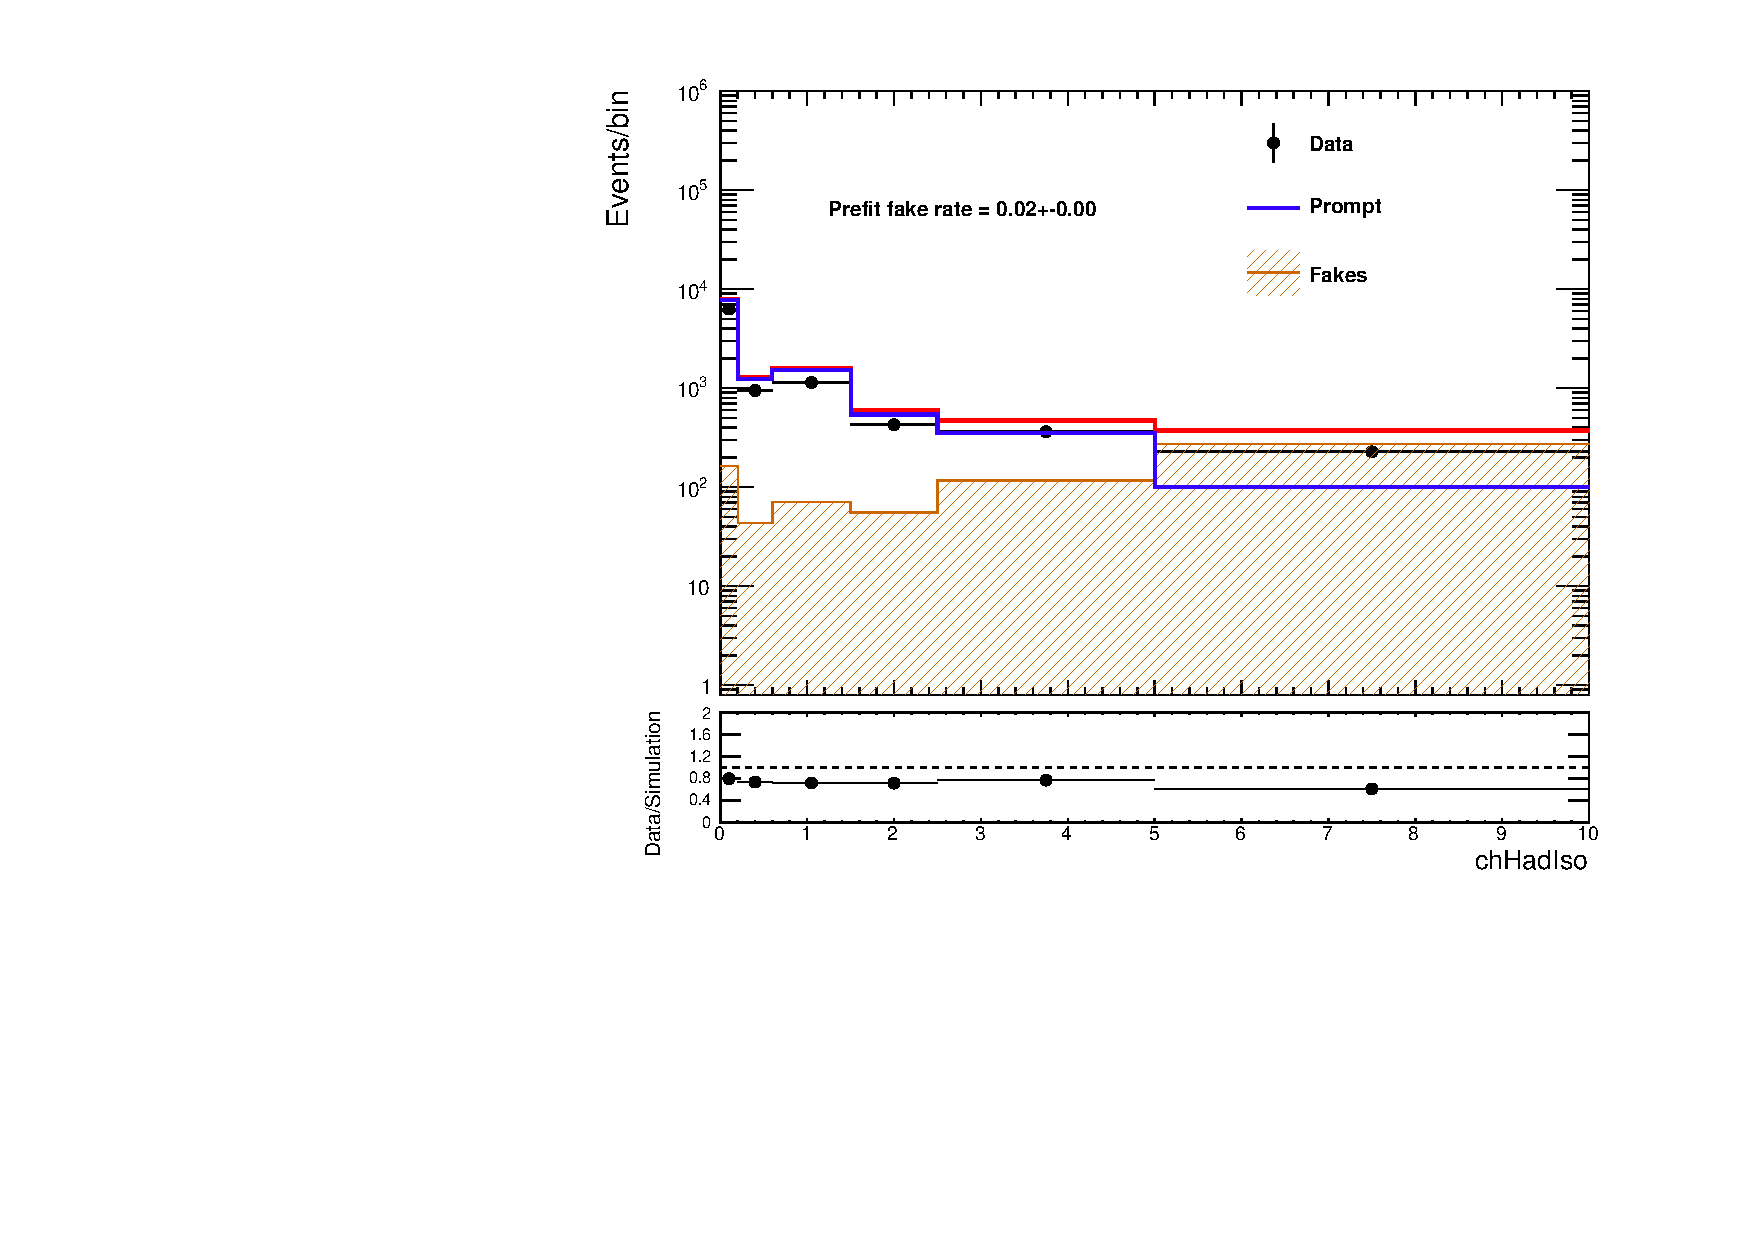
\includegraphics[width=0.45\textwidth]{figures/photonpurity/fakeFit_eq2j_600_prefit} ~
  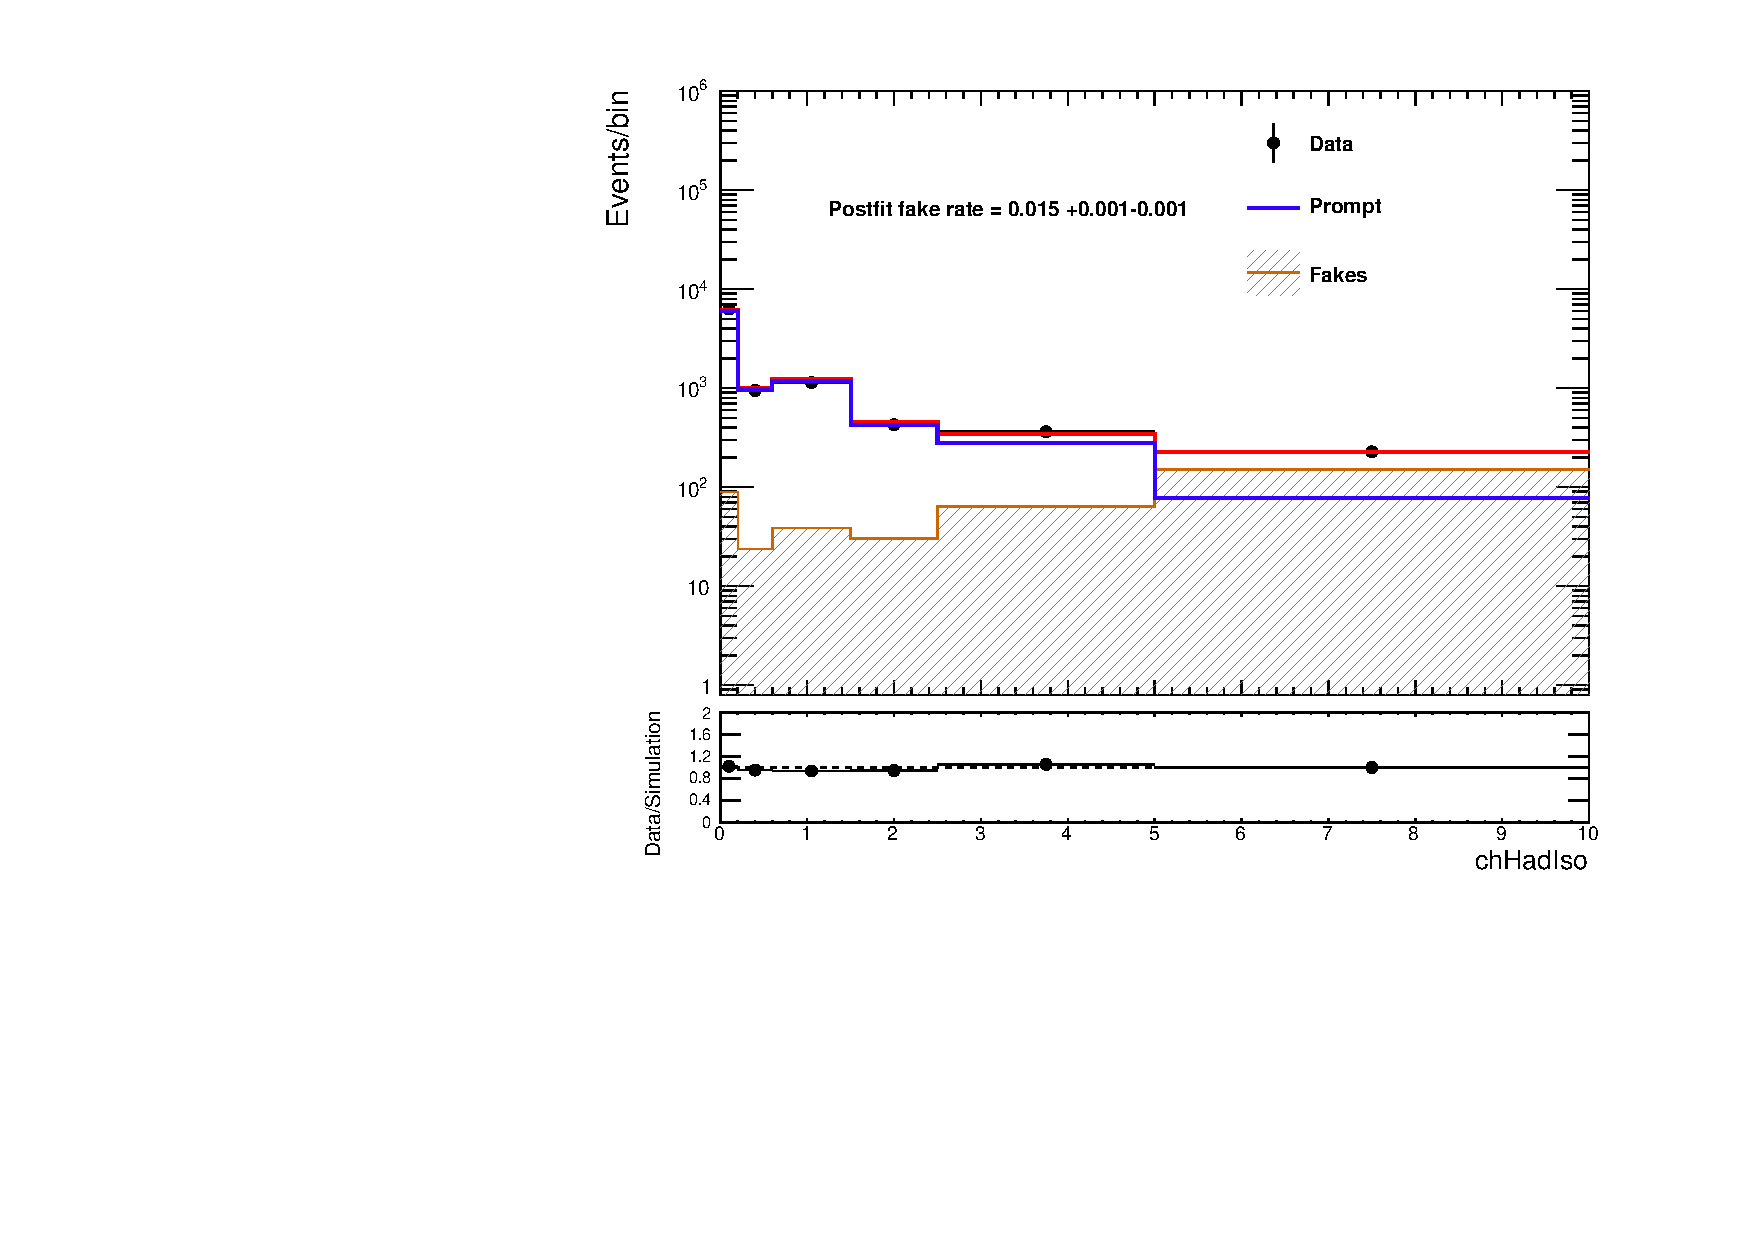
\includegraphics[width=0.45\textwidth]{figures/photonpurity/fakeFit_eq2j_600_postfit} \\
  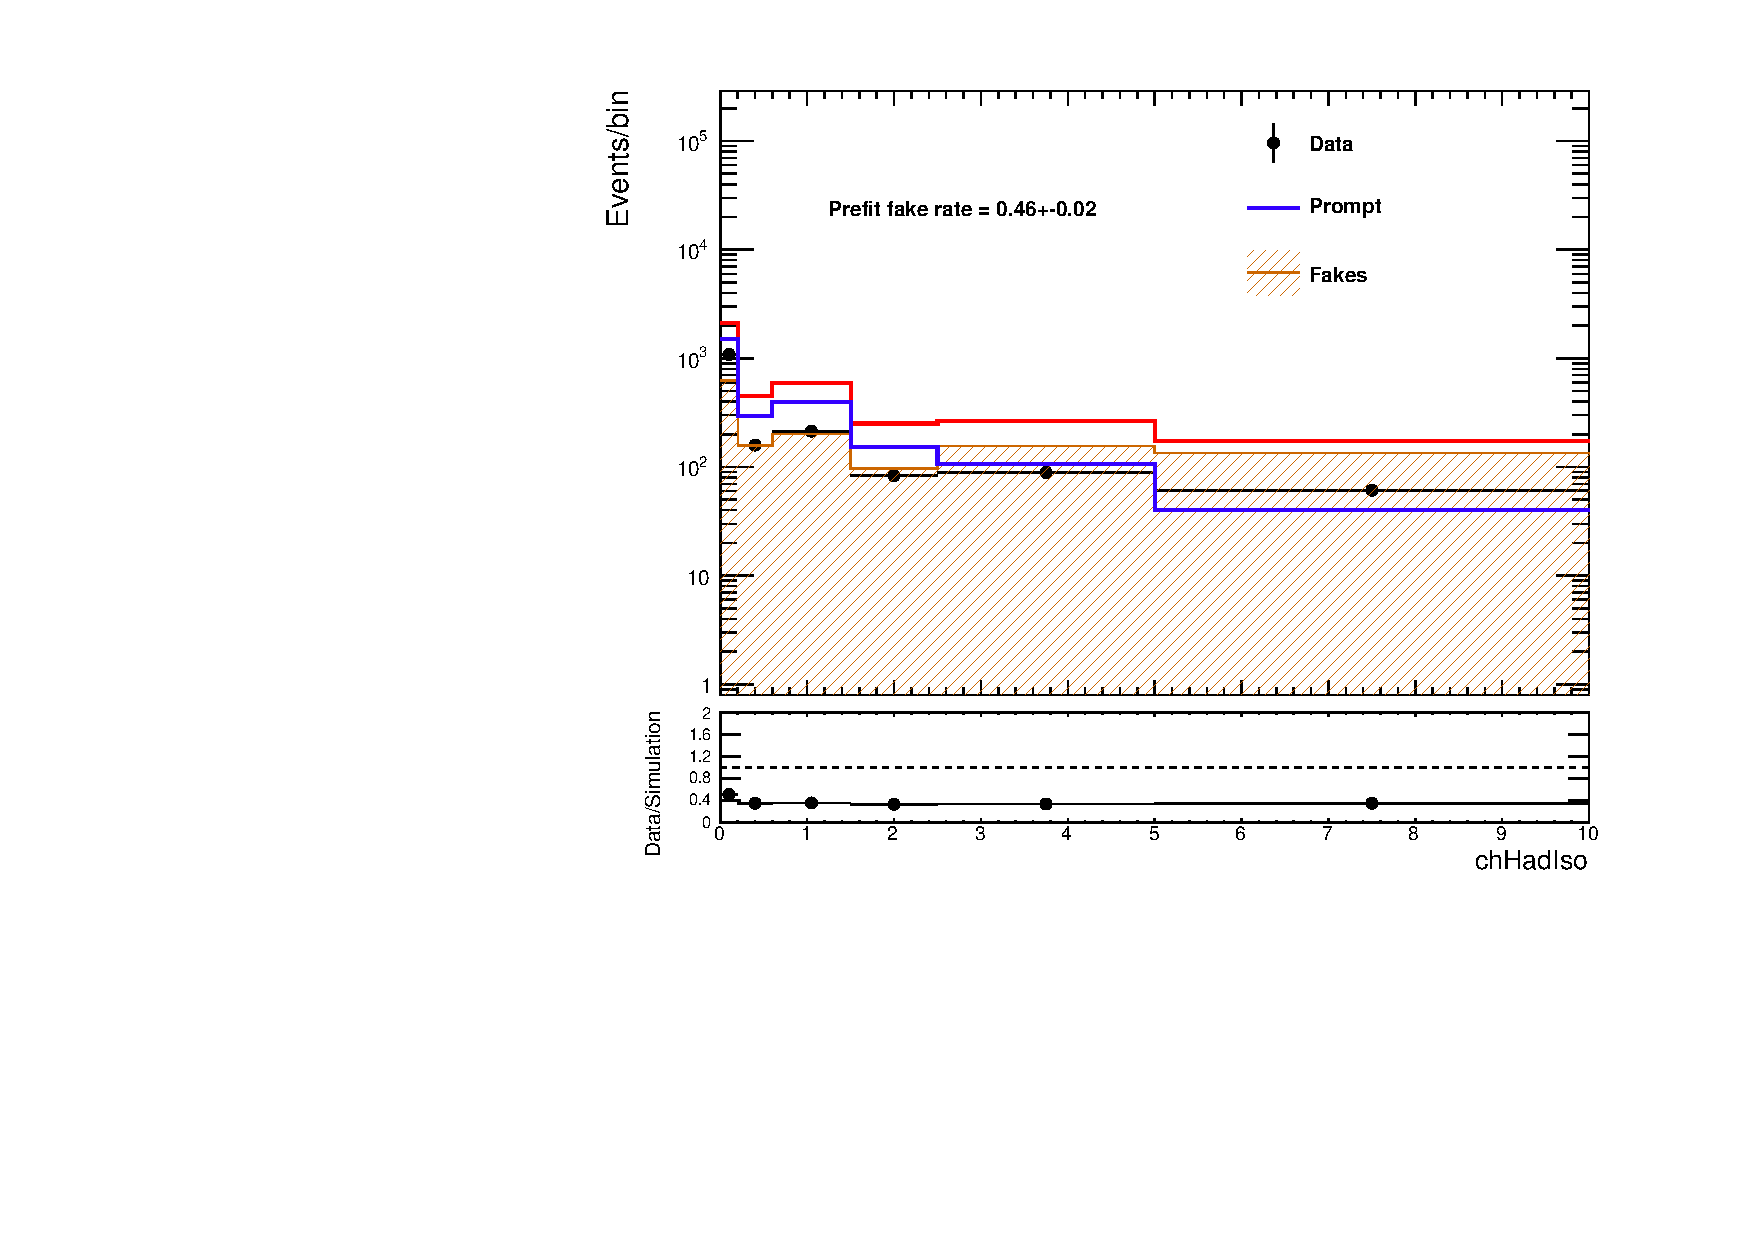
\includegraphics[width=0.45\textwidth]{figures/photonpurity/fakeFit_ge5j_900_prefit} ~
  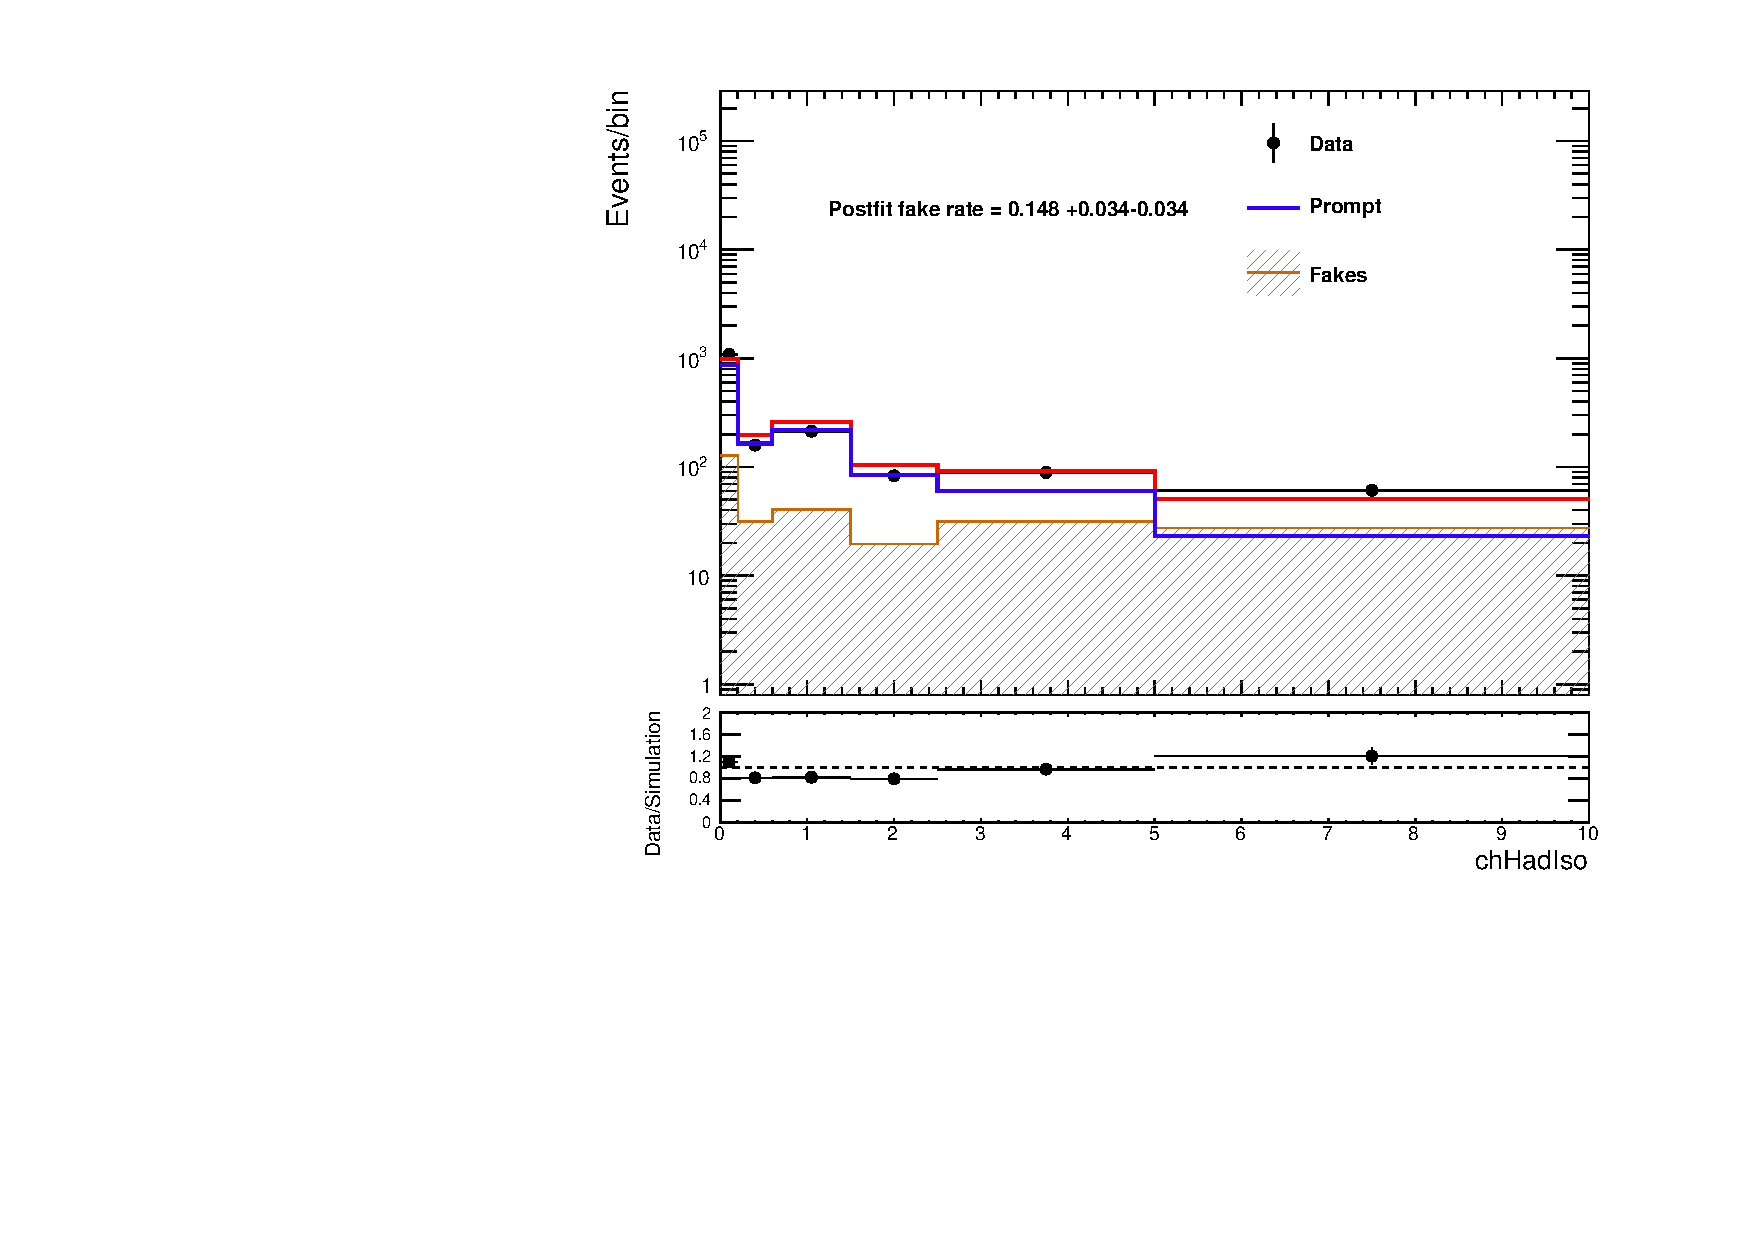
\includegraphics[width=0.45\textwidth]{figures/photonpurity/fakeFit_ge5j_900_postfit}
  \caption{\label{fig:photonTemplateFits} 
  Example prefit (left) and postfit (right) charged hadron isolation
  distributions in the (\njet$=2$, \HT$=600-900$) (top) and 
  (\njet$=5$, \HT$=900-1200$) (bottom) bins.}
\end{figure}


\begin{figure}[h!]
  \centering
  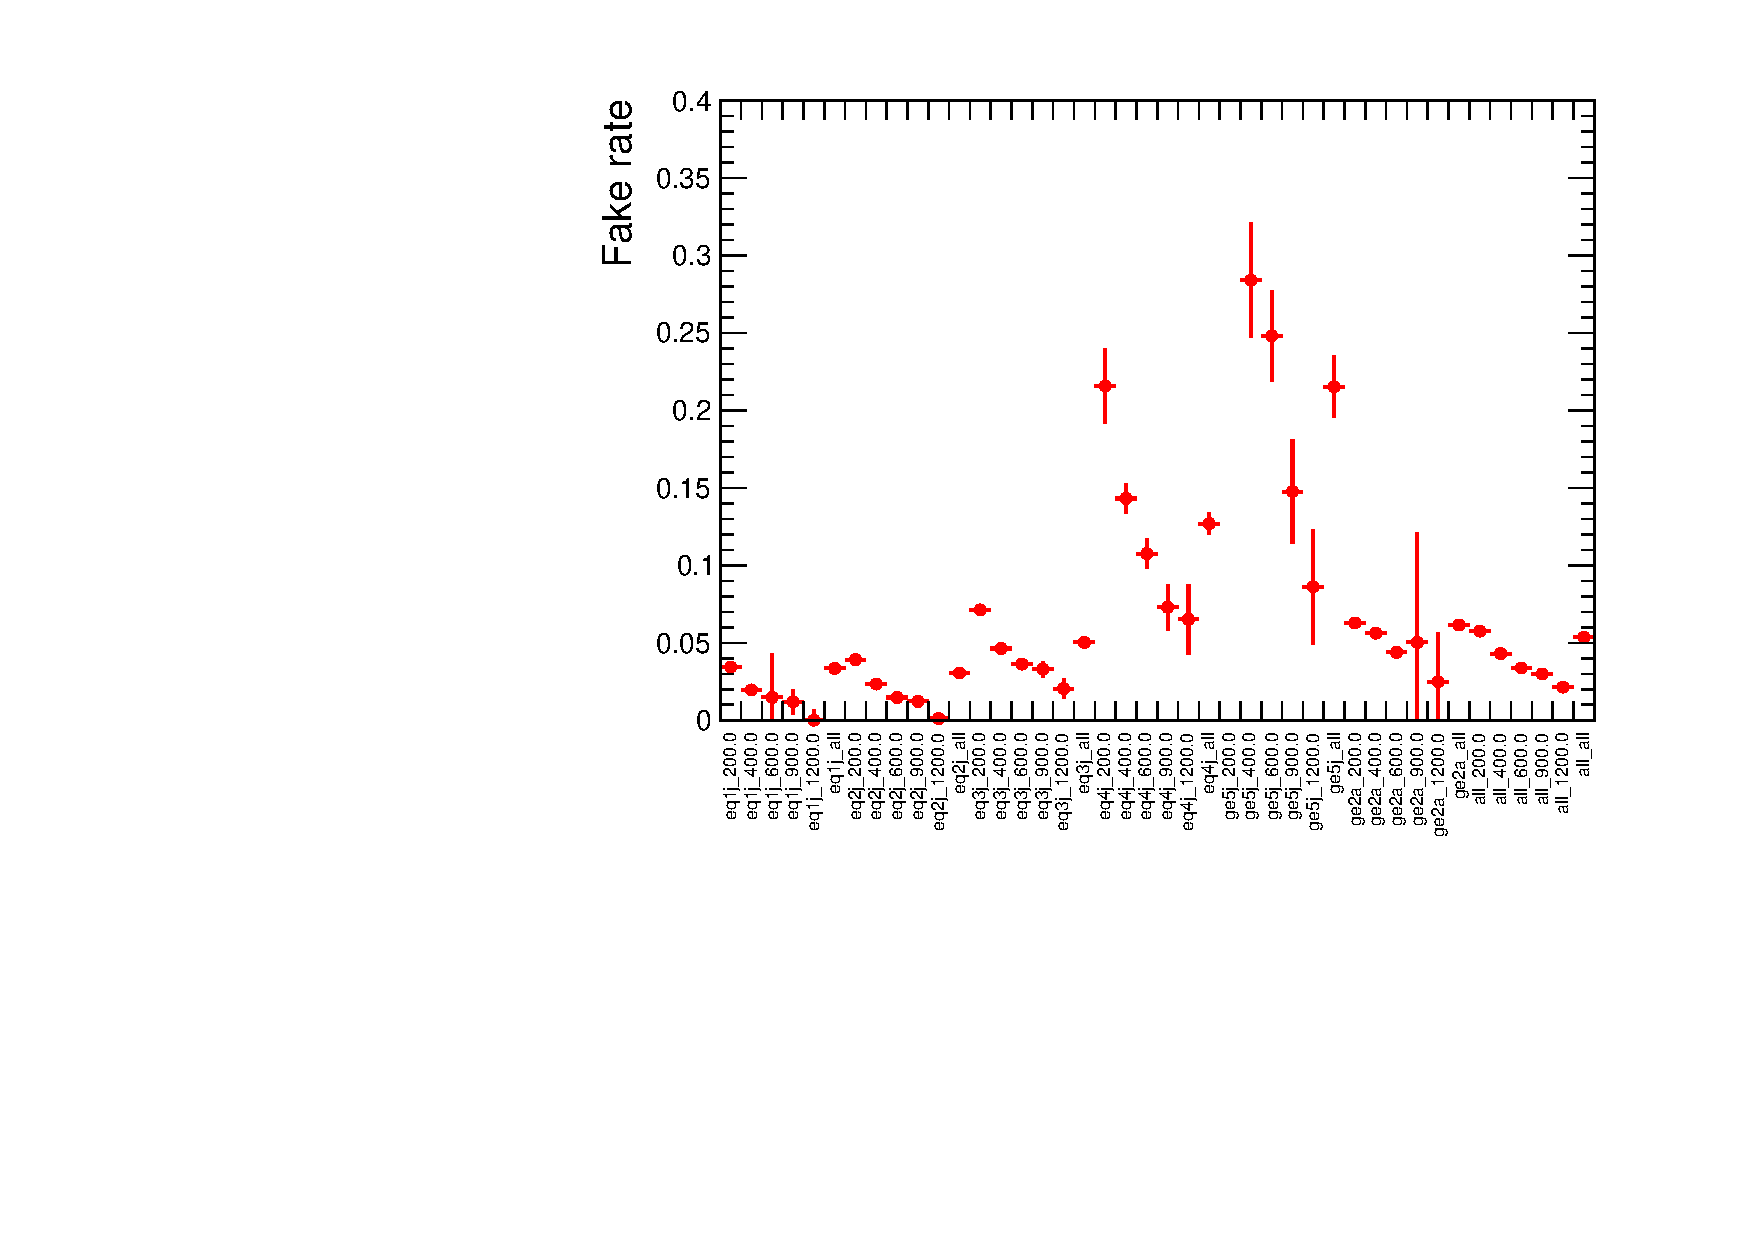
\includegraphics[width=0.45\textwidth]{figures/photonpurity/fake_rate_MC}
  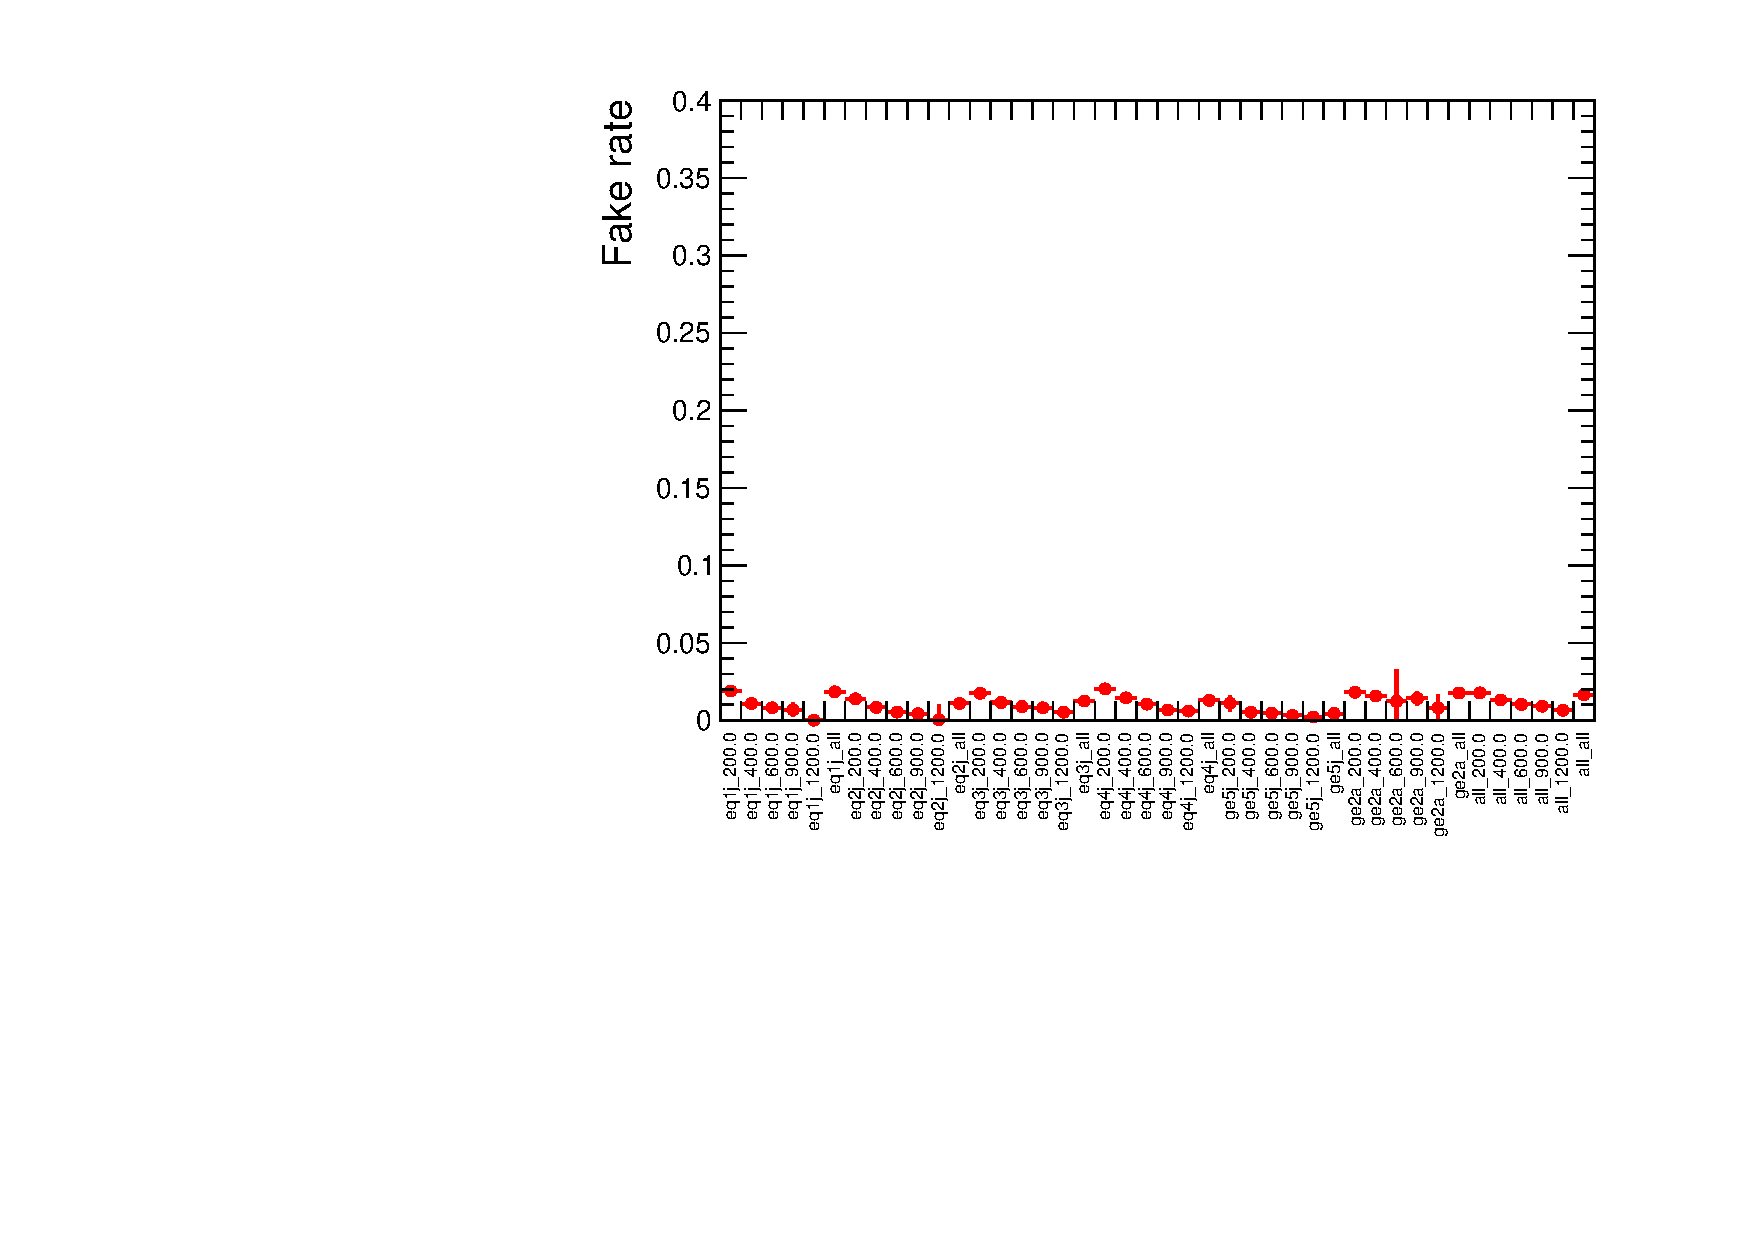
\includegraphics[width=0.45\textwidth]{figures/photonpurity/fake_rate_see}
  \caption{\label{fig:photon-purities} 
  The relative contribution of non-prompt photon as a function
  of (\njet,\HT), when using fakes templates from simulation (left)
  and from the $\sigma_{i\eta i\eta}$ sideband.}
\end{figure}


\subsubsection{Correction to \texorpdfstring{\gj}{photon+jets} cross section}
\label{sec:gj-kfactor}

The \gj cross section used in this analysis is calculated at leading
order, unlike other processes like \ttj (next-to-next-to leading
order) or \zj and \wj (next-to leading order).  A data-driven
procedure is developed to derive a ``k-factor'' for the \gj cross
section by comparing the yields in the \gj and \mmj control regions.
An inclusive correction of 1.39 is derived from the ratio of the event
yields in the two
control regions and is applied to the \gj MC sample. \\
In order to assess the uncertainty on this correction, the systematic
sources affecting the acceptance in the \mmj control region are varied
and the effect on the event yields is derived.  They include lepton
trigger, ID, isolation, tracking efficiency and jet energy
corrections.  The total systematic uncertainty, obtained by summing in
quadrature each independent variation, is 4\% and it's propagated to
the likelihood fit.  Residual discrepancy in the $Z/\gamma$ ratio as a
function of \scalht and \njet are assessed through the data-driven
test described in Sec.~\ref{sec:closure-tests}.


\subsection{The ``transfer factor'' method}
\label{sec:ewk-method}

The method used to estimate the aforementioned SM background
contributions in the hadronic signal region relies on the use of a
transfer factor (TF) determined from MC samples to transform the
observed yield in a given \scalht, jet (\njet) and b-tag (\nb)
multiplicity bin of a control sample, $\nobs^{\rm
  control}(\njet,\nb,\scalht)$, into a predicted yield for the
corresponding bin of the hadronic signal region, $\npre^{\rm
  signal}(\njet,\nb,\scalht)$. The choice of \njet and \nb~event
categorisation and \scalht binning in the control samples is identical
to that for the signal region, as defined in
Sec.~\ref{sec:selection}. 

Each transfer factor is simply a ratio of the yields obtained from MC
simulation for the same bin of the signal region and a given control
sample:

\begin{equation}
  \label{equ:tf-ratio}
  {\rm TF} = \frac{N_{\rm MC}^{\rm signal}(\njet,\nb,\scalht)}{N_{\rm
      MC}^{\rm control}(\njet,\nb,\scalht)} 
\end{equation}

In this way, predictions of background counts from SM processes can be
made based on the various control samples:

\begin{equation}
  \label{equ:pred-method}
  \npre^{\rm signal}(\njet,\nb,\scalht) = \frac{N_{\rm MC}^{\rm
      signal}(\njet,\nb,\scalht)}{N_{\rm MC}^{\rm
      control}(\njet,\nb,\scalht)} \times \nobs^{\rm
    control}(\njet,\nb,\scalht)   
\end{equation}

When constructing the transfer factors, the MC expectations for the
following SM processes are considered: W + jets ($N_{\rm W}$), \ttbar
+ jets ($N_{\ttbar}$), \znunu\ + jets ($N_{\znunu}$), DY + jets
($N_{\mathrm DY}$), \gj ($N_\gamma$), single top + jets
production via the $s$, $t$, and $tW$-channels ($N_{\rm top}$), $WW+$~jets, $WZ~+$~jets, and $ZZ + \textrm{jets}$ ($N_{\rm di-boson}$), and $\ttbar$V or
$\ttbar$H ($N_{\rm {\ttbar}X}$). Details on the MC
samples used are given in Sec.~\ref{sec:datasets}. All MC samples
are normalised to the integrated luminosity of the appropriate data
sample.

The selection criteria for the data control samples closely resemble
those for the signal region, differing mainly through the use of a
lepton or photon object {\it tag} (that is ignored in the calculation
of jet-based kinematic variables such as \scalht, \mht, \alphat, \etc)
and minimal additional kinematic requirements (\eg invariant or
transverse mass windows) to obtain W, Z, and \ttbar-enriched event
samples. The same selection criteria are designed to suppress signal
contamination in the control samples so that unbiased data-driven
estimates for the SM backgrounds in the signal region can be
made. More detail on the selection criteria can be found in Sec.~\ref{sec:selection}.

The transfer factors account for differences in cross sections and
branching ratios, acceptance and reconstruction efficiencies, and/or
kinematic requirements between the signal and control regions. Any
dependence on \njet, \nb, or \HT is largely attributable to
differences in acceptance due to the presence or otherwise of \alphat
or \mht requirements.

Many systematic effects are expected to cancel largely in the transfer
factor. However, a systematic uncertainty is assigned to each transfer
factor to account for theoretical uncertainties and effects such as
the mismodelling of kinematics (\eg acceptances) and instrumental
effects (\eg reconstruction efficiencies).

In the end, a fitting procedure that provides the final result is
defined formally by the likelihood model described in
Sec.~\ref{sec:likelihood}. In summary, the observation in each bin
(defined in terms of the variables \njet, \nb, and \scalht) of the
signal sample is modelled as Poisson-distributed about the sum of a SM
expectation (and a potential signal contribution). The components of
this SM expectation are related to the expected yields in the control
samples via transfer factors derived from simulation. The observations
in each bin (again defined by \njet, \nb, and \scalht) of the control
samples are similarly modelled as Poisson-distributed about the
expected yields for each control sample. In this way, for a given
bin, the observed yields in the signal and control samples are
connected via the transfer factors derived from simulation. 
%% The transfer factors are shown in Tables~\ref{tab:tf_mu_zinv_sym}-
%% \ref{tab:tf_mumu_zinv_mono}. The procedure to determine the systematic
%% uncertainties associated with these transfer factors is described in
%% Sec.~\ref{sec:systematics}. 
The procedure to determine the systematic uncertainties associated
with these transfer factors is described in
Sec.~\ref{sec:systematics}.


%% The transfer factors are shown in tables below.

%% \begin{table}[h!]
\tiny
\centering
\caption{Transfer factors from the \mj control region to the \zInv~ background for symmetric categories.\label{tab:tf_mu_zinv_sym}}
\scalebox{0.85}{\begin{tabular}{ccccccccc}
	\hline\hline
	& \multicolumn{8}{c}{\scalht (\gev)} \\ 
	 (\njet,  \nb) & 200-250 & 250-300 & 300-350 & 350-400 & 400-500 & 500-600 & 600-800 & 800-$\infty$ \\ [0.8ex] 
\hline
	(2, 0) & $1.00\pm 0.02$ & $0.76\pm 0.01$ & $0.57\pm 0.01$ & $0.39\pm 0.01$ & $0.30\pm 0.01$ & $0.21\pm 0.01$ & $0.14\pm 0.00$ & $0.28\pm 0.01$ \\[0.5ex] 
	(2, 1) & $0.48\pm 0.03$ & $0.51\pm 0.02$ & $0.54\pm 0.03$ & $0.44\pm 0.03$ & $0.33\pm 0.02$ & $0.26\pm 0.02$ & $0.20\pm 0.01$ & $0.43\pm 0.03$ \\[0.5ex] 
	(2, 2) & $0.68\pm 0.13$ & $0.77\pm 0.14$ & $0.68\pm 0.14$ & $0.48\pm 0.12$ & $0.33\pm 0.07$ & $0.37\pm 0.12$ & $0.22\pm 0.06$ & -- \\[0.5ex] 
	(3, 0) & $0.19\pm 0.08$ & $0.45\pm 0.01$ & $0.53\pm 0.01$ & $0.53\pm 0.01$ & $0.42\pm 0.01$ & $0.27\pm 0.01$ & $0.19\pm 0.00$ & $0.26\pm 0.00$ \\[0.5ex] 
	(3, 1) & -- & $0.10\pm 0.01$ & $0.16\pm 0.01$ & $0.17\pm 0.01$ & $0.20\pm 0.01$ & $0.18\pm 0.01$ & $0.15\pm 0.01$ & $0.26\pm 0.01$ \\[0.5ex] 
	(3, 2) & -- & $0.08\pm 0.02$ & $0.10\pm 0.01$ & $0.08\pm 0.01$ & $0.08\pm 0.01$ & $0.07\pm 0.01$ & $0.07\pm 0.01$ & $0.14\pm 0.02$ \\[0.5ex] 
	(3, $\ge3$) & -- & -- & -- & -- & $0.03\pm 0.03$ & -- & -- & -- \\[0.5ex] 
	(4, 0) & -- & -- & $0.51\pm 0.03$ & $0.54\pm 0.02$ & $0.44\pm 0.01$ & $0.33\pm 0.01$ & $0.23\pm 0.00$ & $0.24\pm 0.00$ \\[0.5ex] 
	(4, 1) & -- & -- & $0.13\pm 0.01$ & $0.11\pm 0.01$ & $0.11\pm 0.00$ & $0.11\pm 0.01$ & $0.10\pm 0.00$ & $0.17\pm 0.01$ \\[0.5ex] 
	(4, 2) & -- & -- & $0.07\pm 0.02$ & $0.04\pm 0.01$ & $0.05\pm 0.00$ & $0.04\pm 0.00$ & $0.05\pm 0.00$ & $0.09\pm 0.01$ \\[0.5ex] 
	(4, $\ge3$) & -- & -- & -- & $0.06\pm 0.04$ & $0.07\pm 0.02$ & $0.03\pm 0.02$ & $0.03\pm 0.01$ & $0.12\pm 0.05$ \\[0.5ex] 
	($\ge5$, 0) & -- & -- & -- & $0.31\pm 0.04$ & $0.36\pm 0.01$ & $0.27\pm 0.01$ & $0.19\pm 0.00$ & $0.18\pm 0.00$ \\[0.5ex] 
	($\ge5$, 1) & -- & -- & -- & $0.07\pm 0.02$ & $0.07\pm 0.01$ & $0.05\pm 0.00$ & $0.05\pm 0.00$ & $0.06\pm 0.00$ \\[0.5ex] 
	($\ge5$, 2) & -- & -- & -- & $0.01\pm 0.01$ & $0.03\pm 0.00$ & $0.02\pm 0.00$ & $0.02\pm 0.00$ & $0.03\pm 0.00$ \\[0.5ex] 
	($\ge5$, $\ge3$) & -- & -- & -- & -- & $0.03\pm 0.02$ & $0.02\pm 0.01$ & $0.03\pm 0.01$ & $0.03\pm 0.01$ \\[0.5ex] 
	\hline
	\hline
\end{tabular}}
\end{table}

%% \begin{table}[h!]
\tiny
\centering
\caption{Transfer factors from the \mj control region to the \zInv~ background for asymmetric categories. The letter ``a'' in jet \eg ``2a''  indicates the asymmetric jet bins. All entries are non-zero but are truncated to one decimal place.\label{tab:tf_mu_zinv_asym}}
\begin{tabular}
{ccccccccc}
	\hline\hline
&	& \multicolumn{8}{c}{\scalht (\gev)} \\ 
	 (\njet,  \nb) & 200-250 & 250-300 & 300-350 & 350-400 & 400-500 & 500-600 & 600-800 & 800-$\infty$ \\ [0.8ex] 
\hline
	(2a, 0) & $0.55^{+ 0.01 }_{- 0.01 }$ & $0.34^{+ 0.01 }_{- 0.01 }$ & $0.30^{+ 0.01 }_{- 0.01 }$ & $0.30^{+ 0.01 }_{- 0.01 }$ & $0.30^{+ 0.01 }_{- 0.01 }$ & $0.28^{+ 0.01 }_{- 0.01 }$ & $0.25^{+ 0.01 }_{- 0.01 }$ & -- \\[0.5ex] 
	(2a, 1) & $0.22^{+ 0.01 }_{- 0.01 }$ & $0.18^{+ 0.01 }_{- 0.01 }$ & $0.16^{+ 0.01 }_{- 0.01 }$ & $0.21^{+ 0.02 }_{- 0.02 }$ & $0.18^{+ 0.02 }_{- 0.02 }$ & $0.20^{+ 0.03 }_{- 0.03 }$ & $0.19^{+ 0.03 }_{- 0.03 }$ & -- \\[0.5ex] 
	(2a, 2) & $0.21^{+ 0.02 }_{- 0.02 }$ & $0.12^{+ 0.02 }_{- 0.02 }$ & $0.12^{+ 0.03 }_{- 0.03 }$ & $0.07^{+ 0.02 }_{- 0.02 }$ & $0.09^{+ 0.04 }_{- 0.04 }$ & $0.07^{+ 0.05 }_{- 0.05 }$ & $0.07^{+ 0.06 }_{- 0.06 }$ & -- \\[0.5ex] 
	(3a, 0) & $0.57^{+ 0.01 }_{- 0.01 }$ & $0.44^{+ 0.01 }_{- 0.01 }$ & $0.42^{+ 0.01 }_{- 0.01 }$ & $0.32^{+ 0.01 }_{- 0.01 }$ & $0.23^{+ 0.01 }_{- 0.01 }$ & $0.19^{+ 0.01 }_{- 0.01 }$ & $0.18^{+ 0.01 }_{- 0.01 }$ & -- \\[0.5ex] 
	(3a, 1) & $0.10^{+ 0.00 }_{- 0.00 }$ & $0.09^{+ 0.00 }_{- 0.00 }$ & $0.10^{+ 0.00 }_{- 0.00 }$ & $0.10^{+ 0.01 }_{- 0.01 }$ & $0.08^{+ 0.01 }_{- 0.01 }$ & $0.04^{+ 0.01 }_{- 0.01 }$ & $0.06^{+ 0.01 }_{- 0.01 }$ & -- \\[0.5ex] 
	(3a, 2) & $0.04^{+ 0.00 }_{- 0.00 }$ & $0.04^{+ 0.00 }_{- 0.00 }$ & $0.05^{+ 0.01 }_{- 0.01 }$ & $0.03^{+ 0.01 }_{- 0.01 }$ & $0.05^{+ 0.01 }_{- 0.01 }$ & $0.04^{+ 0.02 }_{- 0.02 }$ & $0.03^{+ 0.01 }_{- 0.01 }$ & -- \\[0.5ex] 
	(3a, $\ge3$) & $0.02^{+ 0.01 }_{- 0.01 }$ & $0.04^{+ 0.02 }_{- 0.02 }$ & -- & -- & -- & -- & -- & -- \\[0.5ex] 
	(4a, 0) & $0.16^{+ 0.04 }_{- 0.04 }$ & $0.28^{+ 0.01 }_{- 0.01 }$ & $0.43^{+ 0.01 }_{- 0.01 }$ & $0.42^{+ 0.02 }_{- 0.02 }$ & $0.39^{+ 0.01 }_{- 0.01 }$ & $0.24^{+ 0.02 }_{- 0.02 }$ & $0.15^{+ 0.02 }_{- 0.02 }$ & -- \\[0.5ex] 
	(4a, 1) & $0.02^{+ 0.01 }_{- 0.01 }$ & $0.05^{+ 0.00 }_{- 0.00 }$ & $0.06^{+ 0.00 }_{- 0.00 }$ & $0.07^{+ 0.01 }_{- 0.01 }$ & $0.09^{+ 0.01 }_{- 0.01 }$ & $0.05^{+ 0.01 }_{- 0.01 }$ & $0.04^{+ 0.01 }_{- 0.01 }$ & -- \\[0.5ex] 
	(4a, 2) & -- & $0.03^{+ 0.01 }_{- 0.01 }$ & $0.02^{+ 0.00 }_{- 0.00 }$ & $0.02^{+ 0.00 }_{- 0.00 }$ & $0.03^{+ 0.00 }_{- 0.00 }$ & $0.02^{+ 0.01 }_{- 0.01 }$ & $0.00^{+ 0.00 }_{- 0.00 }$ & -- \\[0.5ex] 
	(4a, $\ge3$) & -- & $0.02^{+ 0.01 }_{- 0.01 }$ & $0.02^{+ 0.01 }_{- 0.01 }$ & $0.02^{+ 0.01 }_{- 0.01 }$ & -- & -- & -- & -- \\[0.5ex] 
	($\ge5$a, 0) & -- & -- & $0.40^{+ 0.04 }_{- 0.04 }$ & $0.38^{+ 0.02 }_{- 0.02 }$ & $0.32^{+ 0.02 }_{- 0.02 }$ & $0.22^{+ 0.02 }_{- 0.02 }$ & $0.21^{+ 0.03 }_{- 0.03 }$ & -- \\[0.5ex] 
	($\ge5$a, 1) & -- & -- & $0.05^{+ 0.01 }_{- 0.01 }$ & $0.05^{+ 0.01 }_{- 0.01 }$ & $0.04^{+ 0.00 }_{- 0.00 }$ & $0.03^{+ 0.01 }_{- 0.01 }$ & $0.02^{+ 0.01 }_{- 0.01 }$ & -- \\[0.5ex] 
	($\ge5$a, 2) & -- & -- & $0.02^{+ 0.01 }_{- 0.01 }$ & $0.02^{+ 0.00 }_{- 0.00 }$ & $0.02^{+ 0.00 }_{- 0.00 }$ & $0.02^{+ 0.00 }_{- 0.00 }$ & $0.01^{+ 0.00 }_{- 0.00 }$ & -- \\[0.5ex] 
	($\ge5$a, $\ge3$) & -- & -- & -- & $0.00^{+ 0.00 }_{- 0.00 }$ & $0.02^{+ 0.01 }_{- 0.01 }$ & $0.03^{+ 0.02 }_{- 0.02 }$ & -- & -- \\[0.5ex] 
	\hline
	\hline
\end{tabular}
\end{table}

%% \begin{table}[h!]
\tiny
\centering
\caption{Transfer factors from the \mj control region to the \zInv~ background for monojet categories.\label{tab:tf_mu_zinv_mono}}
\scalebox{0.85}{\begin{tabular}{ccccccccc}
	\hline\hline
	& \multicolumn{8}{c}{\scalht (\gev)} \\ 
	 (\njet,  \nb) & 200-250 & 250-300 & 300-350 & 350-400 & 400-500 & 500-600 & 600-800 & 800-$\infty$ \\ [0.8ex] 
\hline
	(1, 0) & $1.36\pm 0.01$ & $1.33\pm 0.01$ & $1.30\pm 0.02$ & $1.24\pm 0.02$ & $1.09\pm 0.02$ & $1.17\pm 0.06$ & $1.45\pm 0.17$ & -- \\[0.5ex] 
	(1, 1) & $1.38\pm 0.03$ & $1.45\pm 0.06$ & $1.33\pm 0.08$ & $1.29\pm 0.11$ & $1.11\pm 0.11$ & $0.68\pm 0.15$ & -- & -- \\[0.5ex] 
	\hline
	\hline
\end{tabular}}
\end{table}

%% \begin{table}[h!]
\tiny
\centering
\caption{Transfer factors from the \gj control region to the \zInv~ background for symmetric categories.\label{tab:tf_gj_zinv_sym}}
\scalebox{0.85}{\begin{tabular}{ccccc}
	\hline\hline
	& \multicolumn{4}{c}{\scalht (\gev)} \\ 
	 (\njet,  \nb) & 400-500 & 500-600 & 600-800 & 800-$\infty$ \\ [0.8ex] 
\hline
	(2, 0) & $0.78\pm 0.04$ & $0.72\pm 0.06$ & $0.54\pm 0.04$ & $0.28\pm 0.01$ \\[0.5ex] 
	(2, 1) & $0.82\pm 0.16$ & $0.71\pm 0.20$ & $0.78\pm 0.18$ & $0.24\pm 0.03$ \\[0.5ex] 
	(2, 2) & $0.64\pm 0.42$ & $1.93\pm 1.63$ & $0.52\pm 0.55$ & -- \\[0.5ex] 
	(3, 0) & $0.72\pm 0.04$ & $0.64\pm 0.04$ & $0.67\pm 0.03$ & $0.26\pm 0.01$ \\[0.5ex] 
	(3, 1) & $0.78\pm 0.10$ & $0.68\pm 0.11$ & $1.02\pm 0.17$ & $0.26\pm 0.03$ \\[0.5ex] 
	(3, 2) & $0.71\pm 0.28$ & $0.89\pm 0.55$ & $0.63\pm 0.28$ & $0.21\pm 0.07$ \\[0.5ex] 
	(3, $\ge3$) & -- & -- & -- & -- \\[0.5ex] 
	(4, 0) & $0.83\pm 0.05$ & $0.73\pm 0.05$ & $0.58\pm 0.03$ & $0.27\pm 0.01$ \\[0.5ex] 
	(4, 1) & $0.72\pm 0.11$ & $0.85\pm 0.15$ & $0.69\pm 0.09$ & $0.29\pm 0.03$ \\[0.5ex] 
	(4, 2) & $0.75\pm 0.25$ & $0.70\pm 0.30$ & $0.31\pm 0.10$ & $0.27\pm 0.06$ \\[0.5ex] 
	(4, $\ge3$) & $577.40\pm 664.02$ & $0.38\pm 0.44$ & $0.26\pm 0.31$ & $0.04\pm 0.05$ \\[0.5ex] 
	($\ge5$, 0) & $0.89\pm 0.13$ & $0.71\pm 0.08$ & $0.57\pm 0.04$ & $0.30\pm 0.01$ \\[0.5ex] 
	($\ge5$, 1) & $0.79\pm 0.22$ & $0.57\pm 0.12$ & $0.48\pm 0.07$ & $0.26\pm 0.02$ \\[0.5ex] 
	($\ge5$, 2) & $0.85\pm 0.54$ & $0.40\pm 0.16$ & $0.43\pm 0.15$ & $0.22\pm 0.04$ \\[0.5ex] 
	($\ge5$, $\ge3$) & -- & -- & $1.40\pm 1.47$ & $0.52\pm 0.33$ \\[0.5ex] 
	\hline
	\hline
\end{tabular}}
\end{table}

%% \begin{table}[h!]
\tiny
\centering
\caption{Transfer factors from the \gj control region to the \zInv~ background for asymmetric categories.\label{tab:tf_gj_zinv_asym}}
\begin{tabular}
{ccccc}
	\hline\hline
	& \multicolumn{4}{c}{\scalht (\gev)} \\ 
	 (\njet,  \nb) & 400-500 & 500-600 & 600-800 & 800-$\infty$ \\ [0.8ex] 
\hline
	(2a, 0) & $0.65^{+ 0.05 }_{- 0.05 }$ & $0.56^{+ 0.08 }_{- 0.08 }$ & $0.54^{+ 0.07 }_{- 0.07 }$ & -- \\[0.5ex] 
	(2a, 1) & $1.04^{+ 0.35 }_{- 0.35 }$ & $0.54^{+ 0.24 }_{- 0.24 }$ & -- & -- \\[0.5ex] 
	(2a, 2) & -- & -- & -- & -- \\[0.5ex] 
	(3a, 0) & $0.71^{+ 0.08 }_{- 0.08 }$ & $0.61^{+ 0.12 }_{- 0.12 }$ & $0.76^{+ 0.17 }_{- 0.17 }$ & -- \\[0.5ex] 
	(3a, 1) & $0.68^{+ 0.22 }_{- 0.22 }$ & $0.26^{+ 0.13 }_{- 0.13 }$ & $0.67^{+ 0.45 }_{- 0.45 }$ & -- \\[0.5ex] 
	(3a, 2) & $0.68^{+ 0.43 }_{- 0.43 }$ & $1.08^{+ 1.22 }_{- 1.22 }$ & -- & -- \\[0.5ex] 
	(3a, $\ge3$) & -- & -- & -- & -- \\[0.5ex] 
	(4a, 0) & $0.75^{+ 0.08 }_{- 0.08 }$ & $0.69^{+ 0.15 }_{- 0.15 }$ & $0.42^{+ 0.13 }_{- 0.13 }$ & -- \\[0.5ex] 
	(4a, 1) & $0.87^{+ 0.21 }_{- 0.21 }$ & $0.36^{+ 0.18 }_{- 0.18 }$ & $0.50^{+ 0.36 }_{- 0.36 }$ & -- \\[0.5ex] 
	(4a, 2) & $0.95^{+ 0.63 }_{- 0.63 }$ & -- & -- & -- \\[0.5ex] 
	(4a, $\ge3$) & -- & -- & -- & -- \\[0.5ex] 
	($\ge5$a, 0) & $0.66^{+ 0.09 }_{- 0.09 }$ & $0.69^{+ 0.18 }_{- 0.18 }$ & $0.83^{+ 0.27 }_{- 0.27 }$ & -- \\[0.5ex] 
	($\ge5$a, 1) & $0.84^{+ 0.34 }_{- 0.34 }$ & $0.57^{+ 0.28 }_{- 0.28 }$ & $1.90^{+ 1.88 }_{- 1.88 }$ & -- \\[0.5ex] 
	($\ge5$a, 2) & $0.72^{+ 0.55 }_{- 0.55 }$ & $276.67^{+ 282.97 }_{- 282.97 }$ & -- & -- \\[0.5ex] 
	($\ge5$a, $\ge3$) & -- & -- & -- & -- \\[0.5ex] 
	\hline
	\hline
\end{tabular}
\end{table}

%% \begin{table}[h!]
\tiny
\centering
\caption{Transfer factors from the \gj control region to the \zInv~ background for monojet categories.\label{tab:tf_gj_zinv_mono}}
\begin{tabular}
{ccccc}
	\hline\hline
	& \multicolumn{4}{c}{\scalht (\gev)} \\ 
	 (\njet,  \nb) & 400-500 & 500-600 & 600-800 & 800-$\infty$ \\ [0.8ex] 
\hline
	(1, 0) & $0.57^{+ 0.02 }_{- 0.02 }$ & $0.55^{+ 0.03 }_{- 0.03 }$ & $0.52^{+ 0.03 }_{- 0.03 }$ & -- \\[0.5ex] 
	(1, 1) & $0.59^{+ 0.11 }_{- 0.11 }$ & $0.56^{+ 0.17 }_{- 0.17 }$ & -- & -- \\[0.5ex] 
	\hline
	\hline
\end{tabular}
\end{table}

%% \begin{table}[h!]
\tiny
\centering
\caption{Transfer factors from the \mj control region to the \ttbar/W background for symmetric categories. The letter ``a'' in jet \eg ``2a''  indicates the asymmetric jet bins. All entries are non-zero but are truncated to one decimal place.\label{tab:tf_mu_ttw_sym}}
\begin{tabular}
{ccccccccc}
	\hline\hline
&	& \multicolumn{8}{c}{\scalht (\gev)} \\ 
	 (\njet,  \nb) & 200-250 & 250-300 & 300-350 & 350-400 & 400-500 & 500-600 & 600-800 & 800-$\infty$ \\ [0.8ex] 
\hline
	(2, 0) & $0.9^{+ 0.03 }_{- 0.03 }$ & $0.6^{+ 0.02 }_{- 0.02 }$ & $0.4^{+ 0.02 }_{- 0.02 }$ & $0.3^{+ 0.01 }_{- 0.01 }$ & $0.2^{+ 0.01 }_{- 0.01 }$ & $0.1^{+ 0.01 }_{- 0.01 }$ & $0.1^{+ 0.00 }_{- 0.00 }$ & $0.1^{+ 0.01 }_{- 0.01 }$ \\[0.5ex] 
	(2, 1) & $0.7^{+ 0.04 }_{- 0.04 }$ & $0.5^{+ 0.03 }_{- 0.03 }$ & $0.4^{+ 0.03 }_{- 0.03 }$ & $0.2^{+ 0.03 }_{- 0.03 }$ & $0.1^{+ 0.01 }_{- 0.01 }$ & $0.1^{+ 0.01 }_{- 0.01 }$ & $0.0^{+ 0.01 }_{- 0.01 }$ & $0.1^{+ 0.02 }_{- 0.02 }$ \\[0.5ex] 
	(2, 2) & $0.5^{+ 0.12 }_{- 0.12 }$ & $0.4^{+ 0.09 }_{- 0.09 }$ & $0.4^{+ 0.10 }_{- 0.10 }$ & -- & $0.1^{+ 0.03 }_{- 0.03 }$ & $0.2^{+ 0.06 }_{- 0.06 }$ & $0.0^{+ 0.01 }_{- 0.01 }$ & $0.0^{+ 0.02 }_{- 0.02 }$ \\[0.5ex] 
	(3, 0) & $0.4^{+ 0.22 }_{- 0.22 }$ & $0.4^{+ 0.03 }_{- 0.03 }$ & $0.5^{+ 0.02 }_{- 0.02 }$ & $0.5^{+ 0.02 }_{- 0.02 }$ & $0.3^{+ 0.01 }_{- 0.01 }$ & $0.2^{+ 0.01 }_{- 0.01 }$ & $0.1^{+ 0.00 }_{- 0.00 }$ & $0.1^{+ 0.00 }_{- 0.00 }$ \\[0.5ex] 
	(3, 1) & $0.2^{+ 0.12 }_{- 0.12 }$ & $0.3^{+ 0.02 }_{- 0.02 }$ & $0.3^{+ 0.01 }_{- 0.01 }$ & $0.3^{+ 0.01 }_{- 0.01 }$ & $0.2^{+ 0.01 }_{- 0.01 }$ & $0.1^{+ 0.01 }_{- 0.01 }$ & $0.1^{+ 0.00 }_{- 0.00 }$ & $0.1^{+ 0.01 }_{- 0.01 }$ \\[0.5ex] 
	(3, 2) & -- & $0.2^{+ 0.03 }_{- 0.03 }$ & $0.2^{+ 0.02 }_{- 0.02 }$ & $0.2^{+ 0.02 }_{- 0.02 }$ & $0.1^{+ 0.01 }_{- 0.01 }$ & $0.1^{+ 0.01 }_{- 0.01 }$ & $0.0^{+ 0.01 }_{- 0.01 }$ & $0.0^{+ 0.01 }_{- 0.01 }$ \\[0.5ex] 
	(3, $\ge3$) & -- & -- & -- & $0.4^{+ 0.17 }_{- 0.17 }$ & $0.1^{+ 0.03 }_{- 0.03 }$ & $0.1^{+ 0.04 }_{- 0.04 }$ & -- & -- \\[0.5ex] 
	(4, 0) & -- & -- & $0.7^{+ 0.07 }_{- 0.07 }$ & $0.6^{+ 0.03 }_{- 0.03 }$ & $0.5^{+ 0.01 }_{- 0.01 }$ & $0.3^{+ 0.01 }_{- 0.01 }$ & $0.1^{+ 0.00 }_{- 0.00 }$ & $0.1^{+ 0.00 }_{- 0.00 }$ \\[0.5ex] 
	(4, 1) & -- & -- & $0.4^{+ 0.03 }_{- 0.03 }$ & $0.4^{+ 0.02 }_{- 0.02 }$ & $0.3^{+ 0.01 }_{- 0.01 }$ & $0.1^{+ 0.01 }_{- 0.01 }$ & $0.1^{+ 0.01 }_{- 0.01 }$ & $0.1^{+ 0.01 }_{- 0.01 }$ \\[0.5ex] 
	(4, 2) & -- & -- & $0.4^{+ 0.04 }_{- 0.04 }$ & $0.3^{+ 0.02 }_{- 0.02 }$ & $0.2^{+ 0.01 }_{- 0.01 }$ & $0.1^{+ 0.01 }_{- 0.01 }$ & $0.0^{+ 0.01 }_{- 0.01 }$ & $0.0^{+ 0.01 }_{- 0.01 }$ \\[0.5ex] 
	(4, $\ge3$) & -- & -- & -- & $0.3^{+ 0.06 }_{- 0.06 }$ & $0.3^{+ 0.04 }_{- 0.04 }$ & $0.1^{+ 0.03 }_{- 0.03 }$ & $0.0^{+ 0.01 }_{- 0.01 }$ & $0.0^{+ 0.01 }_{- 0.01 }$ \\[0.5ex] 
	($\ge5$, 0) & -- & -- & -- & $0.5^{+ 0.10 }_{- 0.10 }$ & $0.5^{+ 0.03 }_{- 0.03 }$ & $0.3^{+ 0.01 }_{- 0.01 }$ & $0.2^{+ 0.01 }_{- 0.01 }$ & $0.1^{+ 0.00 }_{- 0.00 }$ \\[0.5ex] 
	($\ge5$, 1) & -- & -- & -- & $0.3^{+ 0.04 }_{- 0.04 }$ & $0.4^{+ 0.01 }_{- 0.01 }$ & $0.2^{+ 0.01 }_{- 0.01 }$ & $0.1^{+ 0.00 }_{- 0.00 }$ & $0.1^{+ 0.00 }_{- 0.00 }$ \\[0.5ex] 
	($\ge5$, 2) & -- & -- & -- & $0.3^{+ 0.05 }_{- 0.05 }$ & $0.3^{+ 0.02 }_{- 0.02 }$ & $0.2^{+ 0.01 }_{- 0.01 }$ & $0.1^{+ 0.00 }_{- 0.00 }$ & $0.1^{+ 0.00 }_{- 0.00 }$ \\[0.5ex] 
	($\ge5$, $\ge3$) & -- & -- & -- & -- & $0.2^{+ 0.04 }_{- 0.04 }$ & $0.2^{+ 0.03 }_{- 0.03 }$ & $0.1^{+ 0.01 }_{- 0.01 }$ & $0.0^{+ 0.01 }_{- 0.01 }$ \\[0.5ex] 
	\hline
	\hline
\end{tabular}
\end{table}

%% \begin{table}[h!]
\tiny
\centering
\caption{Transfer factors from the \mj control region to the \ttbar/W background for asymmetric categories.\label{tab:tf_mu_ttw_asym}}
\scalebox{0.85}{\begin{tabular}{ccccccccc}
	\hline\hline
	& \multicolumn{8}{c}{\scalht (\gev)} \\ 
	 (\njet,  \nb) & 200-250 & 250-300 & 300-350 & 350-400 & 400-500 & 500-600 & 600-800 & 800-$\infty$ \\ [0.8ex] 
\hline
	(2a, 0) & $0.52\pm 0.01$ & $0.27\pm 0.01$ & $0.20\pm 0.01$ & $0.16\pm 0.01$ & $0.12\pm 0.01$ & $0.14\pm 0.02$ & $0.09\pm 0.02$ & -- \\[0.5ex] 
	(2a, 1) & $0.39\pm 0.01$ & $0.22\pm 0.02$ & $0.15\pm 0.02$ & $0.10\pm 0.02$ & $0.12\pm 0.03$ & $0.11\pm 0.05$ & -- & -- \\[0.5ex] 
	(2a, 2) & $0.28\pm 0.04$ & $0.15\pm 0.04$ & $0.16\pm 0.08$ & $0.13\pm 0.09$ & $0.08\pm 0.06$ & -- & -- & -- \\[0.5ex] 
	(3a, 0) & $0.68\pm 0.02$ & $0.50\pm 0.01$ & $0.42\pm 0.02$ & $0.24\pm 0.02$ & $0.13\pm 0.01$ & $0.08\pm 0.01$ & $0.05\pm 0.01$ & -- \\[0.5ex] 
	(3a, 1) & $0.47\pm 0.02$ & $0.36\pm 0.01$ & $0.31\pm 0.02$ & $0.21\pm 0.02$ & $0.09\pm 0.02$ & $0.07\pm 0.02$ & $0.03\pm 0.01$ & -- \\[0.5ex] 
	(3a, 2) & $0.31\pm 0.02$ & $0.24\pm 0.02$ & $0.27\pm 0.02$ & $0.20\pm 0.03$ & $0.04\pm 0.02$ & $0.07\pm 0.06$ & -- & -- \\[0.5ex] 
	(3a, $\ge3$) & $0.19\pm 0.06$ & $0.25\pm 0.06$ & $0.17\pm 0.07$ & -- & -- & -- & -- & -- \\[0.5ex] 
	(4a, 0) & $0.13\pm 0.06$ & $0.46\pm 0.03$ & $0.58\pm 0.03$ & $0.59\pm 0.03$ & $0.35\pm 0.02$ & $0.14\pm 0.02$ & $0.05\pm 0.01$ & -- \\[0.5ex] 
	(4a, 1) & $0.09\pm 0.03$ & $0.23\pm 0.01$ & $0.42\pm 0.02$ & $0.40\pm 0.02$ & $0.29\pm 0.02$ & $0.08\pm 0.02$ & $0.01\pm 0.01$ & -- \\[0.5ex] 
	(4a, 2) & $0.09\pm 0.05$ & $0.16\pm 0.02$ & $0.35\pm 0.02$ & $0.34\pm 0.02$ & $0.24\pm 0.02$ & $0.06\pm 0.02$ & $0.01\pm 0.01$ & -- \\[0.5ex] 
	(4a, $\ge3$) & -- & $0.27\pm 0.09$ & $0.31\pm 0.06$ & $0.27\pm 0.07$ & $0.24\pm 0.08$ & -- & -- & -- \\[0.5ex] 
	($\ge5$a, 0) & -- & $1.81\pm 1.14$ & $0.79\pm 0.11$ & $0.69\pm 0.06$ & $0.64\pm 0.04$ & $0.32\pm 0.04$ & $0.18\pm 0.04$ & -- \\[0.5ex] 
	($\ge5$a, 1) & -- & $0.32\pm 0.13$ & $0.56\pm 0.05$ & $0.51\pm 0.03$ & $0.43\pm 0.02$ & $0.25\pm 0.03$ & $0.08\pm 0.02$ & -- \\[0.5ex] 
	($\ge5$a, 2) & -- & $0.03\pm 0.03$ & $0.49\pm 0.06$ & $0.52\pm 0.04$ & $0.42\pm 0.02$ & $0.18\pm 0.02$ & $0.10\pm 0.03$ & -- \\[0.5ex] 
	($\ge5$a, $\ge3$) & -- & -- & $0.27\pm 0.09$ & $0.39\pm 0.08$ & $0.45\pm 0.07$ & $0.19\pm 0.06$ & -- & -- \\[0.5ex] 
	\hline
	\hline
\end{tabular}}
\end{table}

%% \begin{table}[h!]
\tiny
\centering
\caption{Transfer factors from the \mj control region to the \ttbar/W background for monojet categories.\label{tab:tf_mu_ttw_mono}}
\scalebox{0.85}{\begin{tabular}{ccccccccc}
	\hline\hline
	& \multicolumn{8}{c}{\scalht (\gev)} \\ 
	 (\njet,  \nb) & 200-250 & 250-300 & 300-350 & 350-400 & 400-500 & 500-600 & 600-800 & 800-$\infty$ \\ [0.8ex] 
\hline
	(1, 0) & $1.09\pm 0.01$ & $0.88\pm 0.01$ & $0.74\pm 0.02$ & $0.62\pm 0.02$ & $0.48\pm 0.02$ & $0.40\pm 0.04$ & $0.44\pm 0.09$ & -- \\[0.5ex] 
	(1, 1) & $0.75\pm 0.03$ & $0.77\pm 0.05$ & $0.63\pm 0.06$ & $0.43\pm 0.07$ & $0.66\pm 0.10$ & $0.28\pm 0.10$ & -- & -- \\[0.5ex] 
	\hline
	\hline
\end{tabular}}
\end{table}

%% \begin{table}[h!]
\tiny
\centering
\caption{Transfer factors from the \mmj control region to the \zInv~ background for symmetric categories. The letter ``a'' in jet \eg ``2a''  indicates the asymmetric jet bins. All entries are non-zero but are truncated to one decimal place.\label{tab:tf_mumu_zinv_sym}}
\begin{tabular}
{ccccccccc}
	\hline\hline
&	& \multicolumn{8}{c}{\scalht (\gev)} \\ 
	 (\njet,  \nb) & 200-250 & 250-300 & 300-350 & 350-400 & 400-500 & 500-600 & 600-800 & 800-$\infty$ \\ [0.8ex] 
\hline
	(2, 0) & $9.90^{+ 0.68 }_{- 0.68 }$ & $7.80^{+ 0.44 }_{- 0.44 }$ & $5.05^{+ 0.27 }_{- 0.27 }$ & $4.15^{+ 0.21 }_{- 0.21 }$ & $3.06^{+ 0.09 }_{- 0.09 }$ & $2.16^{+ 0.07 }_{- 0.07 }$ & $1.31^{+ 0.04 }_{- 0.04 }$ & $2.71^{+ 0.09 }_{- 0.09 }$ \\[0.5ex] 
	(2, 1) & $7.16^{+ 1.53 }_{- 1.53 }$ & $4.77^{+ 0.83 }_{- 0.83 }$ & $3.58^{+ 0.60 }_{- 0.60 }$ & $2.98^{+ 0.47 }_{- 0.47 }$ & $2.37^{+ 0.19 }_{- 0.19 }$ & $2.15^{+ 0.24 }_{- 0.24 }$ & $1.53^{+ 0.15 }_{- 0.15 }$ & $2.69^{+ 0.26 }_{- 0.26 }$ \\[0.5ex] 
	(2, 2) & $10.32^{+ 5.34 }_{- 5.34 }$ & $3.33^{+ 1.49 }_{- 1.49 }$ & $7.27^{+ 3.60 }_{- 3.60 }$ & -- & $2.34^{+ 0.87 }_{- 0.87 }$ & $3.46^{+ 1.51 }_{- 1.51 }$ & $1.41^{+ 0.54 }_{- 0.54 }$ & $3.10^{+ 1.89 }_{- 1.89 }$ \\[0.5ex] 
	(3, 0) & $4.98^{+ 4.53 }_{- 4.53 }$ & $6.05^{+ 0.77 }_{- 0.77 }$ & $6.76^{+ 0.50 }_{- 0.50 }$ & $5.94^{+ 0.33 }_{- 0.33 }$ & $4.76^{+ 0.14 }_{- 0.14 }$ & $3.07^{+ 0.09 }_{- 0.09 }$ & $2.00^{+ 0.05 }_{- 0.05 }$ & $2.52^{+ 0.07 }_{- 0.07 }$ \\[0.5ex] 
	(3, 1) & -- & $4.45^{+ 1.07 }_{- 1.07 }$ & $3.74^{+ 0.60 }_{- 0.60 }$ & $4.66^{+ 0.61 }_{- 0.61 }$ & $3.30^{+ 0.27 }_{- 0.27 }$ & $2.22^{+ 0.18 }_{- 0.18 }$ & $1.58^{+ 0.11 }_{- 0.11 }$ & $2.24^{+ 0.17 }_{- 0.17 }$ \\[0.5ex] 
	(3, 2) & -- & $1.17^{+ 0.49 }_{- 0.49 }$ & $2.46^{+ 0.72 }_{- 0.72 }$ & $1.71^{+ 0.43 }_{- 0.43 }$ & $1.71^{+ 0.32 }_{- 0.32 }$ & $1.42^{+ 0.33 }_{- 0.33 }$ & $0.94^{+ 0.20 }_{- 0.20 }$ & $1.69^{+ 0.49 }_{- 0.49 }$ \\[0.5ex] 
	(3, $\ge3$) & -- & -- & -- & $0.76^{+ 0.74 }_{- 0.74 }$ & $0.23^{+ 0.22 }_{- 0.22 }$ & $4.24^{+ 5.21 }_{- 5.21 }$ & -- & -- \\[0.5ex] 
	(4, 0) & -- & -- & $5.24^{+ 1.03 }_{- 1.03 }$ & $7.61^{+ 0.91 }_{- 0.91 }$ & $6.13^{+ 0.26 }_{- 0.26 }$ & $4.15^{+ 0.16 }_{- 0.16 }$ & $2.69^{+ 0.08 }_{- 0.08 }$ & $2.52^{+ 0.09 }_{- 0.09 }$ \\[0.5ex] 
	(4, 1) & -- & -- & $9.05^{+ 4.45 }_{- 4.45 }$ & $6.41^{+ 1.09 }_{- 1.09 }$ & $3.46^{+ 0.35 }_{- 0.35 }$ & $2.75^{+ 0.25 }_{- 0.25 }$ & $1.96^{+ 0.15 }_{- 0.15 }$ & $2.19^{+ 0.16 }_{- 0.16 }$ \\[0.5ex] 
	(4, 2) & -- & -- & $5.02^{+ 2.97 }_{- 2.97 }$ & $1.49^{+ 0.57 }_{- 0.57 }$ & $2.66^{+ 0.50 }_{- 0.50 }$ & $2.11^{+ 0.48 }_{- 0.48 }$ & $1.12^{+ 0.25 }_{- 0.25 }$ & $1.55^{+ 0.28 }_{- 0.28 }$ \\[0.5ex] 
	(4, $\ge3$) & -- & -- & -- & $3.59^{+ 3.91 }_{- 3.91 }$ & $2.82^{+ 1.99 }_{- 1.99 }$ & $2.49^{+ 1.86 }_{- 1.86 }$ & $1.33^{+ 0.94 }_{- 0.94 }$ & $0.36^{+ 0.23 }_{- 0.23 }$ \\[0.5ex] 
	($\ge5$, 0) & -- & -- & -- & $17.39^{+ 6.00 }_{- 6.00 }$ & $6.71^{+ 0.84 }_{- 0.84 }$ & $5.37^{+ 0.35 }_{- 0.35 }$ & $3.23^{+ 0.14 }_{- 0.14 }$ & $2.54^{+ 0.08 }_{- 0.08 }$ \\[0.5ex] 
	($\ge5$, 1) & -- & -- & -- & $4.12^{+ 2.82 }_{- 2.82 }$ & $3.58^{+ 0.70 }_{- 0.70 }$ & $2.65^{+ 0.49 }_{- 0.49 }$ & $2.34^{+ 0.22 }_{- 0.22 }$ & $1.68^{+ 0.11 }_{- 0.11 }$ \\[0.5ex] 
	($\ge5$, 2) & -- & -- & -- & $1.73^{+ 2.20 }_{- 2.20 }$ & $1.53^{+ 0.45 }_{- 0.45 }$ & $1.43^{+ 0.34 }_{- 0.34 }$ & $1.28^{+ 0.26 }_{- 0.26 }$ & $1.02^{+ 0.14 }_{- 0.14 }$ \\[0.5ex] 
	($\ge5$, $\ge3$) & -- & -- & -- & -- & $0.43^{+ 0.37 }_{- 0.37 }$ & $0.88^{+ 0.67 }_{- 0.67 }$ & $2.78^{+ 1.34 }_{- 1.34 }$ & $1.04^{+ 0.45 }_{- 0.45 }$ \\[0.5ex] 
	\hline
	\hline
\end{tabular}
\end{table}

%% \begin{table}[h!]
\tiny
\centering
\caption{Transfer factors from the \mmj control region to the \zInv~ background for asymmetric categories.\label{tab:tf_mumu_zinv_asym}}
\scalebox{0.85}{\begin{tabular}{ccccccccc}
	\hline\hline
	& \multicolumn{8}{c}{\scalht (\gev)} \\ 
	 (\njet,  \nb) & 200-250 & 250-300 & 300-350 & 350-400 & 400-500 & 500-600 & 600-800 & 800-$\infty$ \\ [0.8ex] 
\hline
	(2a, 0) & $5.36^{+ 0.15 }_{- 0.15 }$ & $3.08^{+ 0.12 }_{- 0.12 }$ & $2.45^{+ 0.13 }_{- 0.13 }$ & $2.05^{+ 0.13 }_{- 0.13 }$ & $2.46^{+ 0.13 }_{- 0.13 }$ & $1.78^{+ 0.14 }_{- 0.14 }$ & $1.76^{+ 0.16 }_{- 0.16 }$ & -- \\[0.5ex] 
	(2a, 1) & $3.46^{+ 0.29 }_{- 0.29 }$ & $2.25^{+ 0.26 }_{- 0.26 }$ & $1.72^{+ 0.27 }_{- 0.27 }$ & $2.26^{+ 0.48 }_{- 0.48 }$ & $1.89^{+ 0.30 }_{- 0.30 }$ & $1.73^{+ 0.53 }_{- 0.53 }$ & -- & -- \\[0.5ex] 
	(2a, 2) & $2.78^{+ 0.57 }_{- 0.57 }$ & $1.30^{+ 0.39 }_{- 0.39 }$ & $6.57^{+ 3.34 }_{- 3.34 }$ & $5.82^{+ 6.16 }_{- 6.16 }$ & $1.03^{+ 0.74 }_{- 0.74 }$ & -- & -- & -- \\[0.5ex] 
	(3a, 0) & $7.12^{+ 0.47 }_{- 0.47 }$ & $4.96^{+ 0.26 }_{- 0.26 }$ & $5.25^{+ 0.38 }_{- 0.38 }$ & $3.30^{+ 0.28 }_{- 0.28 }$ & $2.07^{+ 0.13 }_{- 0.13 }$ & $1.42^{+ 0.16 }_{- 0.16 }$ & $1.27^{+ 0.14 }_{- 0.14 }$ & -- \\[0.5ex] 
	(3a, 1) & $4.65^{+ 0.69 }_{- 0.69 }$ & $3.11^{+ 0.37 }_{- 0.37 }$ & $2.74^{+ 0.40 }_{- 0.40 }$ & $2.08^{+ 0.38 }_{- 0.38 }$ & $1.32^{+ 0.22 }_{- 0.22 }$ & $0.43^{+ 0.16 }_{- 0.16 }$ & $1.01^{+ 0.29 }_{- 0.29 }$ & -- \\[0.5ex] 
	(3a, 2) & $2.26^{+ 0.62 }_{- 0.62 }$ & $1.73^{+ 0.43 }_{- 0.43 }$ & $2.34^{+ 0.61 }_{- 0.61 }$ & $2.98^{+ 1.27 }_{- 1.27 }$ & $1.35^{+ 0.47 }_{- 0.47 }$ & $0.99^{+ 0.63 }_{- 0.63 }$ & -- & -- \\[0.5ex] 
	(3a, $\ge3$) & $3.85^{+ 5.06 }_{- 5.06 }$ & $0.85^{+ 0.84 }_{- 0.84 }$ & -- & -- & -- & -- & -- & -- \\[0.5ex] 
	(4a, 0) & $1.39^{+ 0.96 }_{- 0.96 }$ & $4.13^{+ 0.65 }_{- 0.65 }$ & $6.66^{+ 0.77 }_{- 0.77 }$ & $6.56^{+ 0.78 }_{- 0.78 }$ & $5.00^{+ 0.46 }_{- 0.46 }$ & $2.29^{+ 0.38 }_{- 0.38 }$ & $1.19^{+ 0.22 }_{- 0.22 }$ & -- \\[0.5ex] 
	(4a, 1) & $1.10^{+ 1.24 }_{- 1.24 }$ & $3.82^{+ 1.30 }_{- 1.30 }$ & $3.23^{+ 0.68 }_{- 0.68 }$ & $3.84^{+ 0.95 }_{- 0.95 }$ & $3.63^{+ 0.58 }_{- 0.58 }$ & $1.86^{+ 0.61 }_{- 0.61 }$ & $0.67^{+ 0.31 }_{- 0.31 }$ & -- \\[0.5ex] 
	(4a, 2) & -- & $7.92^{+ 4.39 }_{- 4.39 }$ & $3.58^{+ 1.20 }_{- 1.20 }$ & $4.29^{+ 1.67 }_{- 1.67 }$ & $3.07^{+ 1.14 }_{- 1.14 }$ & $0.32^{+ 0.24 }_{- 0.24 }$ & $0.00^{+ 0.01 }_{- 0.01 }$ & -- \\[0.5ex] 
	(4a, $\ge3$) & -- & $10318.30^{+ 14528.12 }_{- 14528.12 }$ & $3.56^{+ 3.40 }_{- 3.40 }$ & -- & -- & -- & -- & -- \\[0.5ex] 
	($\ge5$a, 0) & -- & -- & $7.38^{+ 3.65 }_{- 3.65 }$ & $8.54^{+ 2.29 }_{- 2.29 }$ & $6.86^{+ 1.21 }_{- 1.21 }$ & $3.67^{+ 0.60 }_{- 0.60 }$ & $2.75^{+ 0.58 }_{- 0.58 }$ & -- \\[0.5ex] 
	($\ge5$a, 1) & -- & -- & $5.59^{+ 3.26 }_{- 3.26 }$ & $2.76^{+ 1.02 }_{- 1.02 }$ & $2.89^{+ 0.68 }_{- 0.68 }$ & $3.67^{+ 1.46 }_{- 1.46 }$ & $1.21^{+ 0.58 }_{- 0.58 }$ & -- \\[0.5ex] 
	($\ge5$a, 2) & -- & -- & $9.13^{+ 10.19 }_{- 10.19 }$ & $7.66^{+ 5.88 }_{- 5.88 }$ & $3.05^{+ 1.26 }_{- 1.26 }$ & $2.85^{+ 1.66 }_{- 1.66 }$ & $0.25^{+ 0.27 }_{- 0.27 }$ & -- \\[0.5ex] 
	($\ge5$a, $\ge3$) & -- & -- & -- & -- & $1.40^{+ 1.34 }_{- 1.34 }$ & $81.43^{+ 112.36 }_{- 112.36 }$ & -- & -- \\[0.5ex] 
	\hline
	\hline
\end{tabular}}
\end{table}

%% \begin{table}[h!]
\tiny
\centering
\caption{Transfer factors from the \mmj control region to the \zInv~ background for monojet categories.\label{tab:tf_mumu_zinv_mono}}
\begin{tabular}
{ccccccccc}
	\hline\hline
	& \multicolumn{8}{c}{\scalht (\gev)} \\ 
	 (\njet,  \nb) & 200-250 & 250-300 & 300-350 & 350-400 & 400-500 & 500-600 & 600-800 & 800-$\infty$ \\ [0.8ex] 
\hline
	(1, 0) & $11.96^{+ 0.31 }_{- 0.31 }$ & $10.23^{+ 0.40 }_{- 0.40 }$ & $9.84^{+ 0.55 }_{- 0.55 }$ & $9.47^{+ 0.66 }_{- 0.66 }$ & $8.75^{+ 0.45 }_{- 0.45 }$ & $8.71^{+ 0.52 }_{- 0.52 }$ & $8.19^{+ 0.52 }_{- 0.52 }$ & -- \\[0.5ex] 
	(1, 1) & $9.75^{+ 1.12 }_{- 1.12 }$ & $8.00^{+ 1.31 }_{- 1.31 }$ & $6.45^{+ 1.39 }_{- 1.39 }$ & $6.84^{+ 1.86 }_{- 1.86 }$ & $9.69^{+ 2.68 }_{- 2.68 }$ & $9.37^{+ 2.61 }_{- 2.61 }$ & -- & -- \\[0.5ex] 
	\hline
	\hline
\end{tabular}
\end{table}


%% \clearpage

\subsection{Adding the \mht dimension}

The aforementioned description of the TFs provide an estimate of the
total SM background as a function of the (\njet,\nb,\HT) bin that is
integrated over \mht. However, the analysis takes advantage of \mht
distribution obtained from simulation. This information is propagated
to the likelihood model via an \mht template per (\njet,\nb,\HT) bin,
which is equivalent to dicing the numerator of the TF according to
\mht, \ie $N_{\rm MC}^{\rm signal}(\njet,\nb,\scalht,\mht)$. In this
regard, the TFs described above provide an estimate of the
normalisation for each \mht template.

%\subsection{Data control samples used in the method}
%
%To estimate the contributions from backgrounds with genuine missing
%transverse momentum, three data control regions are used, which are
%binned identically to the signal region: \mj, \mmj and \gj.  Their
%definitions are provided in Sec.~\ref{sec:selection}. The selection
%criteria for these control regions are defined such that any potential
%contamination from new physics processes or QCD multijets is
%negligible.

%% In previous versions of this analysis, the \mmj and \gj control
%% samples are used to predict the \znunu +jets background. We plan to
%% extend this approach by relying on all (and not just a sub-set of)
%% relevant control samples to predict the two dominant components of the
%% total SM background (\wj and \ttbar, or \znunu + jets). Specifically,
%% we are using the \mj sample to predict the \wj and \ttbar backgrounds
%% (across all \nb bins) and up to three samples comprising \zmmj,
%% \gj and \wmj to predict the \znunu + jets background for events
%% containing exactly zero or one b-tagged jets. Any correlations are
%% appropriately handled by the likelihood model (via the
%% \texttt{Combine} tool).

%% The predictions of the \znunu + jets background based on the \zmmj
%% control samples exhibits significantly larger statistical
%% uncertainties at high \njet, \nb, \scalht, or \mht due to lower event
%% counts arising from the lower Z cross section (w.r.t. \gj and
%% \wj). Regardless, these samples are included in the likelihood fit
%% to provide additional confidence in the control of the \znunu + jets
%% background.

%% Concerning the use of $W$-enriched samples to predict the \znunu +jets
%% background, we have studied this approach
%% in detail with the 8\TeV dataset. Based on the outcome of these studies,
%% we have decided to proceed with this approach, as part
%% of the baseline likelihood description. Studies were
%% based on data-driven tests with 8\TeV data
%% (as described in Sec.~\ref{sec:closure-tests}). Closure tests are a critical
%% tool to determine which samples can be used to predict the SM
%% background components. In particular, we have studied the effect of
%% new closure tests designed to test the $W$-enriched to $Z$-enriched
%% extrapolation, specifically \mj to \gj, \mj to \mmj
%% and $\mu^{+}$ to $\mu^{-}$ closure tests. 
%% If further studies of the closure tests with $13\tev$
%% data suggest that using the \mj control region to predict the \znunu
%% background is not feasible, we will revert back to the approach
%% used in Run~I analysis (\ie relying solely on the \zll and \gj
%% samples). Early investigations suggest there are not any major problems.
%% %The closure tests provide important event samples for probing the
%% %accuracy of the simulation modelling implicit in the transfer factors.
%% %Specific examples include ``\mj to predict \mmj'' and ``zeej to
%% %predict \gj'' with events containing exactly zero or one b-tagged
%% %jets. The former test relies on a \wmj-enriched sample to predict
%% %yields in the \zmmj sample (in the presence of some ``\ttbar
%% %contamination'' for events with $\nb = 1$). The latter test is a
%% %consistency check between a dilepton and a \gj sample (as done in
%% %previous iterations of the analysis).
%% Most importantly, we retain full flexibility in our approach and the
%% control samples used to predict the various background components.

%% Currently, the projected sensitivity, as described in the current
%% version of this note, is based on predictions of SM background
%% components made from control regions as follows. For events containing
%% exactly zero or one b-tagged jets, the \mj (enriched in \wej), \gj and
%% \mmj control samples are used to estimate the irreducible \znunu + jets
%% background, while the \mj control sample is used to estimate all
%% remaining SM processes (predominately \wj and \ttbar). For events
%% containing two or more b-tagged jets, the \mj sample is
%% used to predict the total SM background (dominated by \ttbar).


%%%%____________________________________________________________________________||
\clearpage
\section{Systematic uncertainties in the transfer factors}
\label{sec:systematics}

This section addresses the estimation of systematic uncertainties
affecting the transfer factors (equation~\ref{equ:tf-ratio})
for non-multijet backgrounds. 
These uncertainties will be often referred to as \textit{``normalisation uncertainties''}, 
as opposed to the \textit{``template uncertainties''} described in Sec.~\ref{sec:syst-on-shape}. 
The former affect the total number of events in each (\njet,~\nb,~\scalht) bin (integrating over \mht), 
while the latter encode the limited knowledge on how these events distribute in the \mht dimension.

Two approaches are used to derive uncertainties from specific sources:
one is based on variations in simulation (Sec.~\ref{sec:mc-variations}), the other makes use of control samples in data (Sec.~\ref{sec:closure-tests}).
Each systematic source considered in the analysis is described below, 
together with the method used to derive the corresponding uncertainties and the correlation model. 
A summary of the all the uncertainties is given in Tab.~\ref{tab:systs}.

%%%%%%%%%%%%%%%%%%%%%%%%%%%%%%%%%%%%%%%%%%%%%%%%%%%%%%%%%%%%%%%
% MC-based systematics
%%%%%%%%%%%%%%%%%%%%%%%%%%%%%%%%%%%%%%%%%%%%%%%%%%%%%%%%%%%%%%%
\subsection{Systematic variations in simulation}
\label{sec:mc-variations}

A set of corrections are applied to the MC samples in order to improve the modelling 
of detector effects (b-tagging efficiency, jet energy response, etc.) 
as well as the simulation of the kinematics of certain processes (top $p_{T}$). 
These corrections are described in Sec.~\ref{sec:datasets}. \\
In this section the effect of varying these corrections within their uncertainties is 
presented, focusing on the relative change in the 4 type of transfer factors which are of interest 
for the background prediction, namely: $\mj \rightarrow (\znunu)$,
$\mmj \rightarrow (\znunu)$, $\gj \rightarrow (\znunu)$ and $\mj
\rightarrow \mathrm{\ttbar+W}$. 
The binning of the analysis is chosen in order to minimise the impact of 
these systematic sources, which are expected to be sub-dominant. 
However, they are propagated to the final results, taking into account
correlations and bin migration effects. 
The magnitude of the uncertainties are summarised in Table~\ref{tab:systs} at
the end of this section. 

All figures referenced in this sub-section can be found in Appendix~\ref{app:systematics}.

\subsubsection*{Jet energy scale}
\label{sec:tfSyst_jec}
The effect of varying the jet energy scale in
the \mj and \mmj control regions is investigated.  The energies of
jets used in the analysis are corrected as a function of their \pt and
$\eta$ via the procedure recommended by the JetMET POG. These
corrections have an associated uncertainty, which is propagated through the analysis. 
As the \scalht and jet multiplicity binning is mirrored in signal and control regions, 
the effect of jet energy scale on the transfer factor is expected to be small. 
However, the jet energy scale can still have an
effect due to jets moving in and out acceptance (above and below
$40\gev$). The relative change in the transfer factors is presented as a function of \scalht and jet category 
in Fig. ~\ref{fig:tfSyst_jec_muToZinv}-\ref{fig:tfSyst_jec_muToTtw}.
The changes are typically in the range of $1-5\%$.

\subsubsection*{B-tagging efficiency}
\label{sec:tfSyst_btag}

Scale factors provided by the BTV POG are applied to the MC samples
to correct for differences in the b-tagging efficiencies and 
misidentifications between simulation and data. 
The method employed is based on simple event reweighting as described in
Ref.~\cite{btagSFMethods}. 
Events are reweighted according to the probability of obtaining a particular jet configuration in data
and simulation, as determined by the b-tagging efficiencies computed
in the MC samples and the scale factors measured in data.
Since no extrapolation is performed in the background prediction across different 
\nb multiplicities, the analysis is expected to be robust against variations in the 
b-tagging efficiency. 
To test this effect the change in the transfer factors is measured
by varying the scale factors within their uncertainties. The scale factors
associated with b and c jets are varied together (since their measurements are
correlated), while those associated with light jets are varied separately.
The relative change in the transfer factors is presented as a function of \scalht and jet category 
in Fig. ~\ref{fig:tfSyst_bsf_muToZinv}-\ref{fig:tfSyst_bsfl_muToTtw}.
They are typically in the range of $1-3\%$.

\subsubsection*{Lepton and photon trigger/identification/isolation efficiency}
\label{sec:leptonSyst}
Leptons out of $p_{T}$ and $\eta$ acceptance, or within detector
acceptance but not identified properly by lepton identification or isolation
requirements contribute to the so-called ``lost-lepton background'', 
which mainly stem from W and \ttbar events. 
The fraction of events with leptons out of acceptance (\flepAccep)
is calculated from generator truth level information for each MC
sample. Differences in efficiencies between data and simulation are
accounted for with data/MC scale
factors for trigger, lepton identification and isolation~\cite{twiki-leptonSF}, 
and change the lost lepton background in the signal region and yields in 
muon control regions simultaneously.

The effect of lepton reconstruction on the lost lepton background
can be summarised in the following expressions respectively:
\begin{equation}
    \label{eq:lostLepSR}
    \sum_{sample} [ R_{sample} \times \flepAccep \times N^{GEN}_{sample} \times ( 1 - \epsilon_{Loose} ) + ( 1 - \flepAccep ) \times N^{GEN}_{sample} ]
\end{equation}
\begin{equation}
    \label{eq:lostLepCR}
    \sum_{sample} N^{GEN}_{sample} \times \epsilon_{Tight} \times R_{sample}
\end{equation}
where $R_{sample}$ is the cross section reweighting factor for each sample, 
$N^{GEN}_{sample}$ is the total MC events for the category, $\epsilon_{Tight}$
and $\epsilon_{Loose}$ are the lepton efficiency for Tight and Loose working 
point. For the numerator, full
signal selection except the lepton veto to mimic signal region phase space as
closely as possible. For the denominator, the full selection for the \mj 
control sample is applied.

The systematic variations on the signal region and control region are computed 
by varying the lepton scale factor
up and down according to each source of uncertainty.
Data/MC lepton scale factors have negligible statistical uncertainties. 
The procedure is repeated separately for muons and
electrons.
A log-normal systematic uncertainty of 5\% is assigned to $\mathrm{tt+W}$ in the signal region, 
and one with 2\% to the control region. The two systematics are taken to be anti-correlated 
with each other.

Finally, the $\eta$-dependent muon tracking scale factors provided by the muon 
POG to cover the effect of HIP inefficiencies have been applied and their 
uncertainties taken into consideration. Their effect on the transfer factors
is found to be less than 1\%.

\subsubsection*{Lepton Acceptance}
Theoretical uncertainties from parton distribution function and factorisation can 
introduce systematic uncertaintes on lepton acceptance, i.e. the fraction of leptons out 
of $p_{T}$ or $\eta$ range. The effect can then be parametrized with the variable \flepAccep 
in Section~\ref{sec:leptonSyst}
Theoretical uncertainties from parton distribution function
are varied according to the recommended prescription from PDF4LHC~\cite{PDF4LHC:2015}. The systematic variations 
are found to be less than 1\%.

\subsubsection*{Photon trigger uncertainty}
\label{sec:tfSyst_photonTrigger}

Variations in the trigger weight for the signal region are studied. A conservative systematic
uncertainty on this correction is taken as the size of the inefficiency. 
The relative change in the \gj transfer factor is presented in Fig.~\ref{fig:tfSyst_photonTrigger_gjToZinv}
variation is typically in the range $0-3\%$.

\subsubsection*{Signal trigger uncertainty}
\label{sec:tfSyst_trigger}

Variations in the trigger weight for the signal region are studied. A systematic is taken
as the difference in the efficiency measured using muon and electron reference triggers.
The relative change in the transfer factors is typically in the range
$1-7\%$, as presented in Figs.
~\ref{fig:tfSyst_trigger_muToZinv}-\ref{fig:tfSyst_trigger_muToTtw}, 

%\subsubsection*{Top $p_T$ reweighting}
%\label{sec:tfSyst_topPt}
%
%Variations in the reweighting of top $p_{T}$ distribution, as first outlined in 
%Sec.~\ref{sec:SMxs}, are studied. A conservative systematic
%uncertainty on this correction is taken as the size of the correction itself. 
%The relative change in transfer factors is presented in Fig.
%~\ref{fig:tfSyst_topPt_muToZinv}-\ref{fig:tfSyst_topPt_muToTtw}. The
%variation is typically in the range $0-15\%$.

%\subsubsection*{QCD contamination}
%\label{sec:tfSyst_qcdCont}
%
%A check has also been performed on the systematic effect on the
%background prediction due to QCD contamination in the control samples,
%which has been found to be at the ~5\% level for the \gj
%control region. Applying an arbitrarily large variation of $\pm
%100\%$ on the number of Monte Carlo QCD events leads to a systematic
%variation on the transfer factors of at most 5\% in the majority of bins.
%This preliminary study suggests that effect from QCD
%contamination in the \gj control region is small compared 
%to the total uncertainty assigned to transfer factors. 
%This systematic source is covered in the data-driven study  
%using the photon control region, described in Sec. ~\ref{sec:tfSyst_ZGratio}.

\subsubsection*{PU reweighting}
\label{sec:tfSyst_pu}

Events in simulation are reweighted in order to match the distribution 
of the primary vertex multiplicity observed in data, as described in Sec. ~\ref{sec:pileup-reweighting}.
A systematic uncertainty is derived by propagating 
the 5\% uncertainty on the minimum bias cross section used in the reweighting procedure. 
The relative change in the transfer factors under this variation is
small (\~1-7\%)
and shown in each analysis bin in Fig. ~\ref{fig:tfSyst_pu_muToZinv}-\ref{fig:tfSyst_pu_muToTtw}.

%\clearpage
%% %%%%%%%%%%%%%%%%%%%%%%%%%%%%%%%%%%%%%%%%%%%%%%%%%%%%%%%%%%%%%%%%
%% % Closure tests
%% %%%%%%%%%%%%%%%%%%%%%%%%%%%%%%%%%%%%%%%%%%%%%%%%%%%%%%%%%%%%%%%%

\subsection{Systematics uncertainties from data-driven tests}
\label{sec:closure-tests}
This analysis aims to rely as much as possible on the data control samples
to check for sources of bias in the transfer factors due to potential limitations in
the simulation modelling. 
Therefore, along with the MC variations mentioned above, tests are performed 
in which the number of events in a given data control sample is predicted 
using events from another data control sample and the corresponding transfer factor built in MC. 
The agreement between the predicted and observed yields is
expressed as the ratio $(\nobs - \npre)/\npre$ while considering only
the statistical uncertainties on \npre and \nobs. Therefore, the level
of closure is defined by the statistical significance of a deviation
in the ratio from zero.
These tests are performed separately for each \njet category, as a function of \scalht. 
The systematic uncertainty in each \scalht bin is derived by summing in quadrature the ratio 
defined above with its statistical error, after merging the \njet categories into symmetric and asymmetric topologies. 
Pairs of \scalht bins are merged when the $\mu\mu$+jets sample is used, in order to gain statistics. 
These systematics are considered un-correlated in each \scalht bin and jet topology. 
The magnitude of the uncertainties are summarised in Table~\ref{tab:systs} at
the end of this section. 

\subsubsection*{Extrapolation in \alphat and \bdphi}
\label{sec:tfSyst_alphaT}
The modelling of the \alphat and
\bdphi extrapolations are also tested with dedicated tests in data. 
In both cases, it is checked that events with genuine \met found in the core
of the variable distribution below some threshold value can be used to
predict the events in the tail (above the same threshold value).
This is important to verify the
approach of using \mj and \mmj samples without an \alphat requirement
to make background predictions in the signal region. The tests
confront data yields in a \mj  samples with an \alphat /\bdphi
requirement against predictions determined in a \mj sample with
the \alphat /\bdphi requirement inverted. 
The contribution to the systematic error for \met extrapolation is taken
from the \alphat closure tests for bins with $\scalht<800\gev$ and from 
the \bdphi tests for bins with $\scalht>800\gev$. 

The result of these tests are shown in Figs.~\ref{fig:closureAlphaT}
and~\ref{fig:closure_bdphi} as a function of \scalht and \njet. 
The grey band is the systematic uncertainty propagated through the analysis, 
taken as un-correlated per each \scalht bin and jet topology
(symmetric/asymmetric). The systematic derived from these tests is
in the range $3-20\%$.

\subsubsection*{Modelling of the W/Z ratio}
\label{sec:tfSyst_WZratio}
To validate the use of \wmj and \ttbar dominated \mj events to predict the \znunu
background, tests are performed in data using single-muon and double-muon control regions. 
The events in the \mj control are used to predict events in the \mmj control regions, 
using transfer factors from simulation. 
These tests target the modelling of the W/Z ratio in simulation and 
also indirectly test muon acceptance effects, which 
are expected to be sub-dominant and whose uncertainties are already addressed elsewhere.

The result are shown in Fig.~\ref{fig:closureMuToMuMu} as a function of \scalht and \njet. 
The grey band is the systematic uncertainty propagated through the analysis, 
taken as un-correlated per each \scalht bin and jet topology (symmetric/asymmetric). The systematic derived from these tests is
in the range $1-12\%$.

\subsubsection*{Modelling of the W/Z acceptance due to polarisation effects}
\label{sec:tfSyst_Wpol}
A data-driven test is introduced to check the modelling of the W polarisation in simulation. 
In this study, carried on using events in the single-muon control region, $\mu^{+}$ events 
are used to predict $\mu^{-}$ events, using transfer factor built in MC. 
The polarisation of the W boson has an impact on the prediction 
of the \znunu background using the \mj control region, as explained in the following. 
The production mechanism of $W$ from pp
collisions means high $p_T$ $W$ bosons are predominantly left handed
\cite{WPol}.  For high $p_T$ bosons, this implies that $W^+$ decays to
the left handed neutrino along its direction of motion while the
lepton is pointing backward. The opposite behaviour is expected for
the $W^-$. The lepton is therefore more boosted (and the neutrino less
boosted) in $W^+$ decays than $W^-$ decays.  This leads to a larger
number of $W^+$ decays in the single lepton control regions (which
relies on the lepton $p_T$ for acceptance) than in the signal region
(which relies on the neutrino $p_T$ for acceptance).

The results are shown in Fig.~\ref{fig:closureMuPToMuM} as a function of \scalht and \njet. 
The grey band is the systematic uncertainty propagated through the analysis, 
taken as un-correlated per each \scalht bin and jet topology (symmetric/asymmetric). The systematic derived from these tests is
in the range $2-14\%$.

\subsubsection*{Modelling of the Z/$\gamma$ ratio}
\label{sec:tfSyst_ZGratio}
To validate the use of \gj events to predict the \znunu
background, tests are performed in data using the photon and double-muon control regions. 
The events in the \gj control are used to predict events in the \mmj control regions, 
using transfer factors from simulation. 
These tests target the modelling of the Z/$\gamma$ ratio in simulation and 
also indirectly test muon/photon acceptance effects, which, however, 
are expected to be sub-dominant and whose uncertainties are already addressed elsewhere. 

The result are shown in Fig.~\ref{fig:closurePhoToMuMu} as a function of \scalht and \njet. 
The grey band is the systematic uncertainty propagated through the analysis, 
taken as un-correlated per each \scalht bin and jet topology (symmetric/asymmetric). The systematic derived from these tests is
in the range $2-26\%$.

\subsubsection*{Modelling of the W/\ttbar admixture}
\label{sec:tfSyst_WttAd}
The $0$ b-tag $\rightarrow1$ b-tag data-driven tests in the \mj control region 
probe the sensitivity of the transfer factors to the relative
admixture of events from the $W$ + jets and \ttbar processes, 
since they utilise a W-enriched sample to predict a \ttbar-enriched sample. 
These tests indirectly probe also the modelling of the b-tagging
efficiency and the related scale factor corrections;
however, the ICHEP16 b-tag SF are applied, discussed in \ref{sec:inputs-and-updates},
thus the derived systematic is not propagated to the fit. Instead this
closure tests is inspected solely as a cross-check. 
%These tests indirectly probe also the modelling of the b-tagging efficiency, 
%although this systematic effect is expected to be smaller and is already addressed 
%by the dedicated study presented in Sec. ~\ref{sec:tfSyst_btag}.
%These tests are believed to give a conservative uncertainty, 
%as the admixture changes little between the \mj sample and the signal region, 
%given that no extrapolation between different b-tag multiplicities is performed 
%in the estimation of the background. 
%The uncertainty derived is therefore driven by the limited statistics available in the control sample. 
The result are shown in Fig.~\ref{fig:closureBTag} as a function of \scalht and \njet. 
%The grey band is the systematic uncertainty.% propagated through the analysis, 
%taken as un-correlated per each \scalht bin and jet topology (symmetric/asymmetric). The systematic derived from these tests is
%in the range $4-25\%$.

\begin{figure}[h!]
  \begin{center}
    \subfigure[]{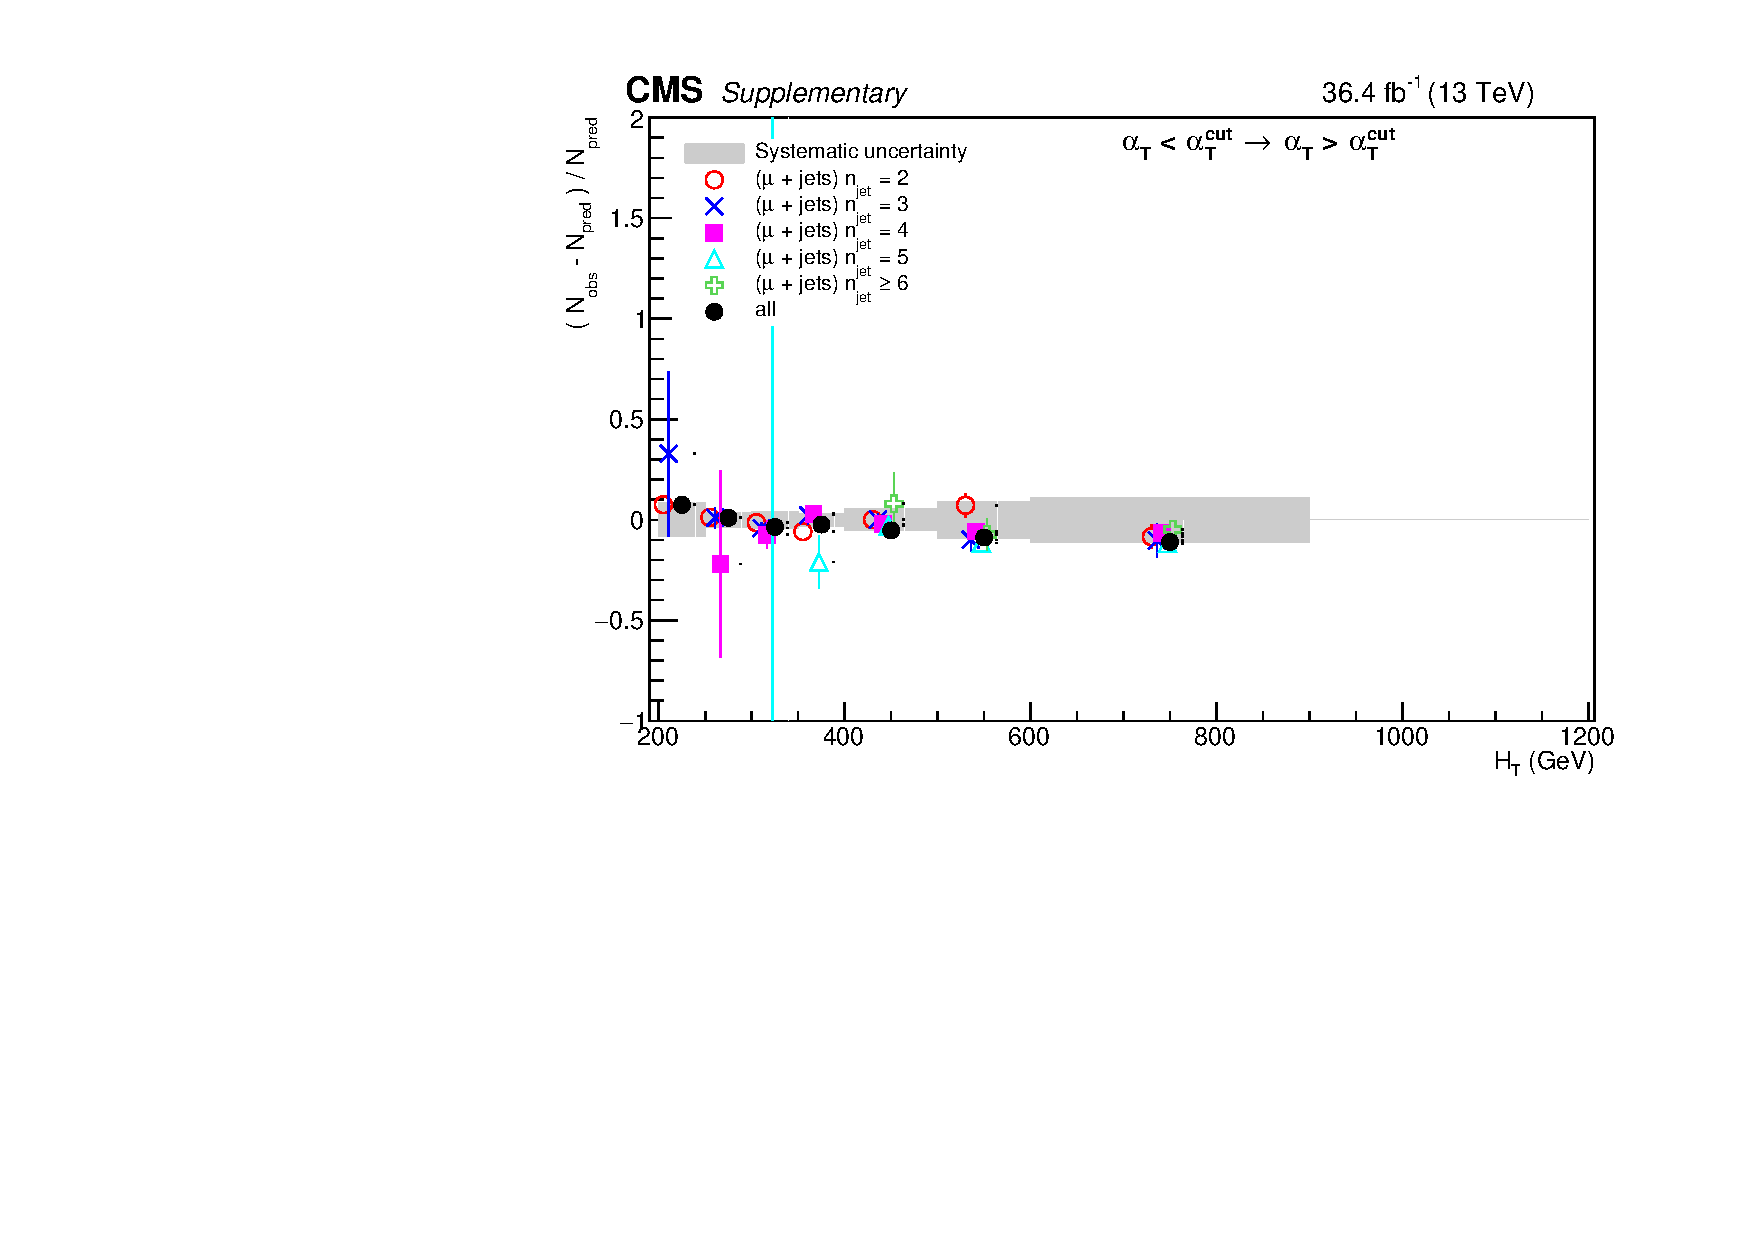
\includegraphics[width=0.5\textwidth]{figures/closureTests/alphaT_mu_sym__noFit.pdf}}
    ~~
    \subfigure[]{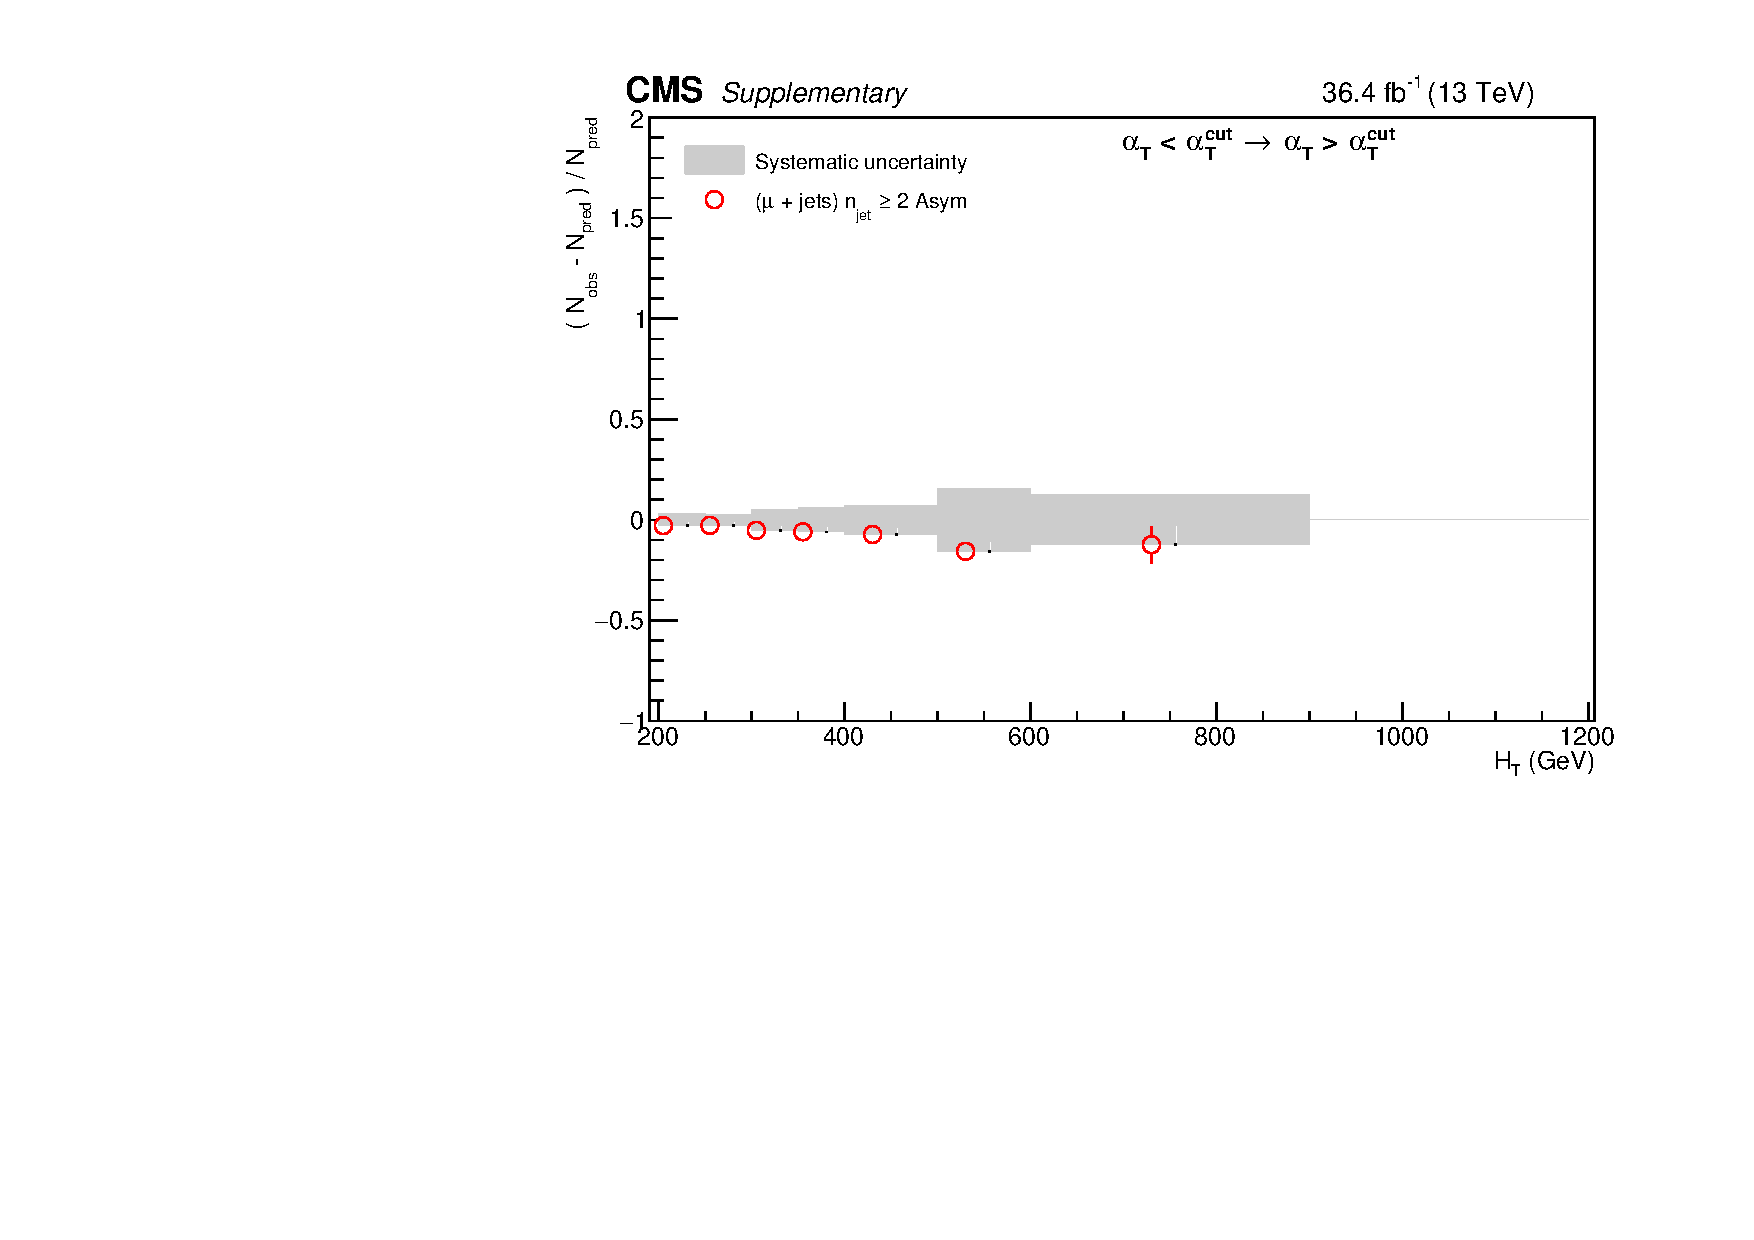
\includegraphics[width=0.5\textwidth]{figures/closureTests/alphaT_mu_asym__noFit.pdf}}
    \caption{Data-driven tests probing the \alphat extrapolation for each
      \njet category (open symbols) overlaid on top of the systematic
      uncertainty estimates used for each \scalht bin (shaded bands). 
      The symmetric (asymmetric) jet topologies are shown in the left (right) plot. 
    }
    \label{fig:closureAlphaT}
  \end{center} 
\end{figure}

\begin{figure}[h!]
  \begin{center}
    \subfigure[]{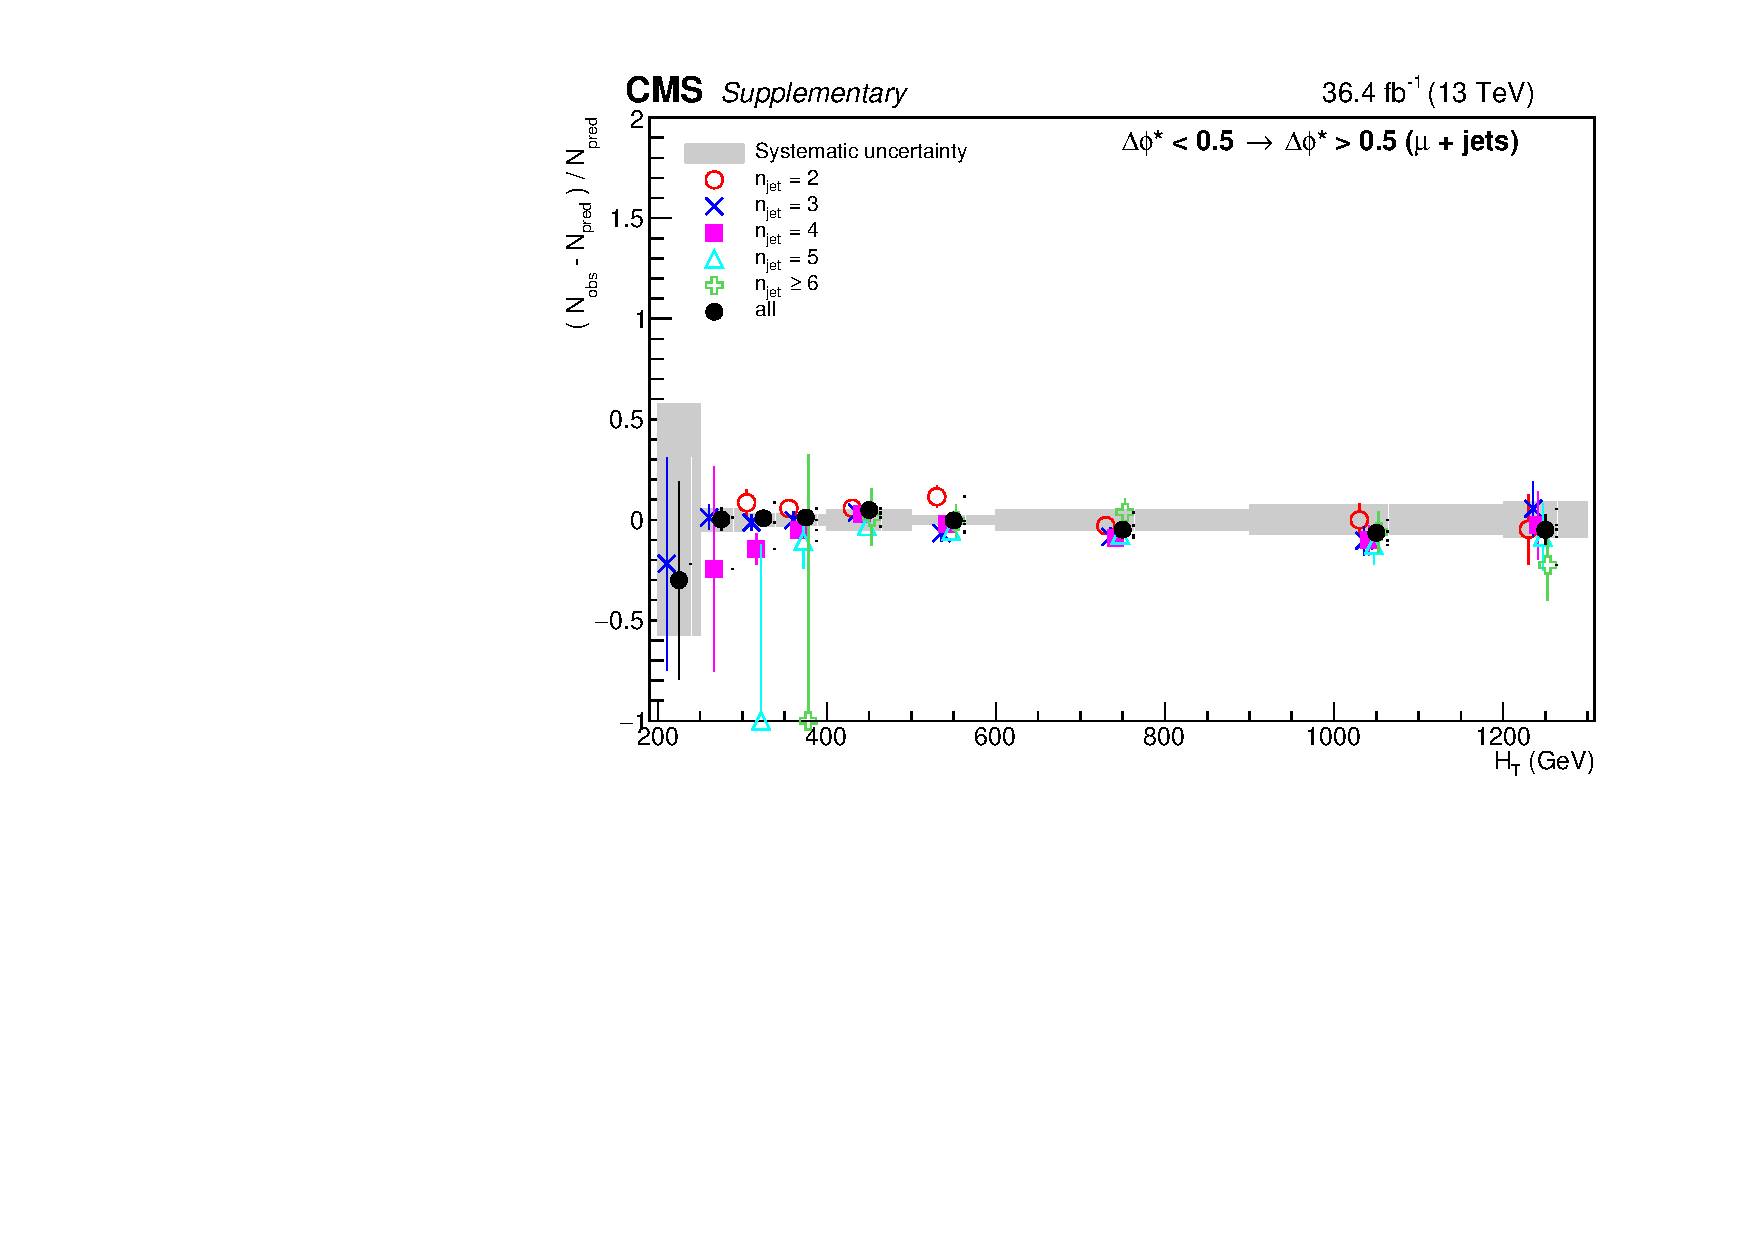
\includegraphics[width=0.5\textwidth]{figures/closureTests/bDPhi_sym__noFit.pdf}}
    ~~
    \subfigure[]{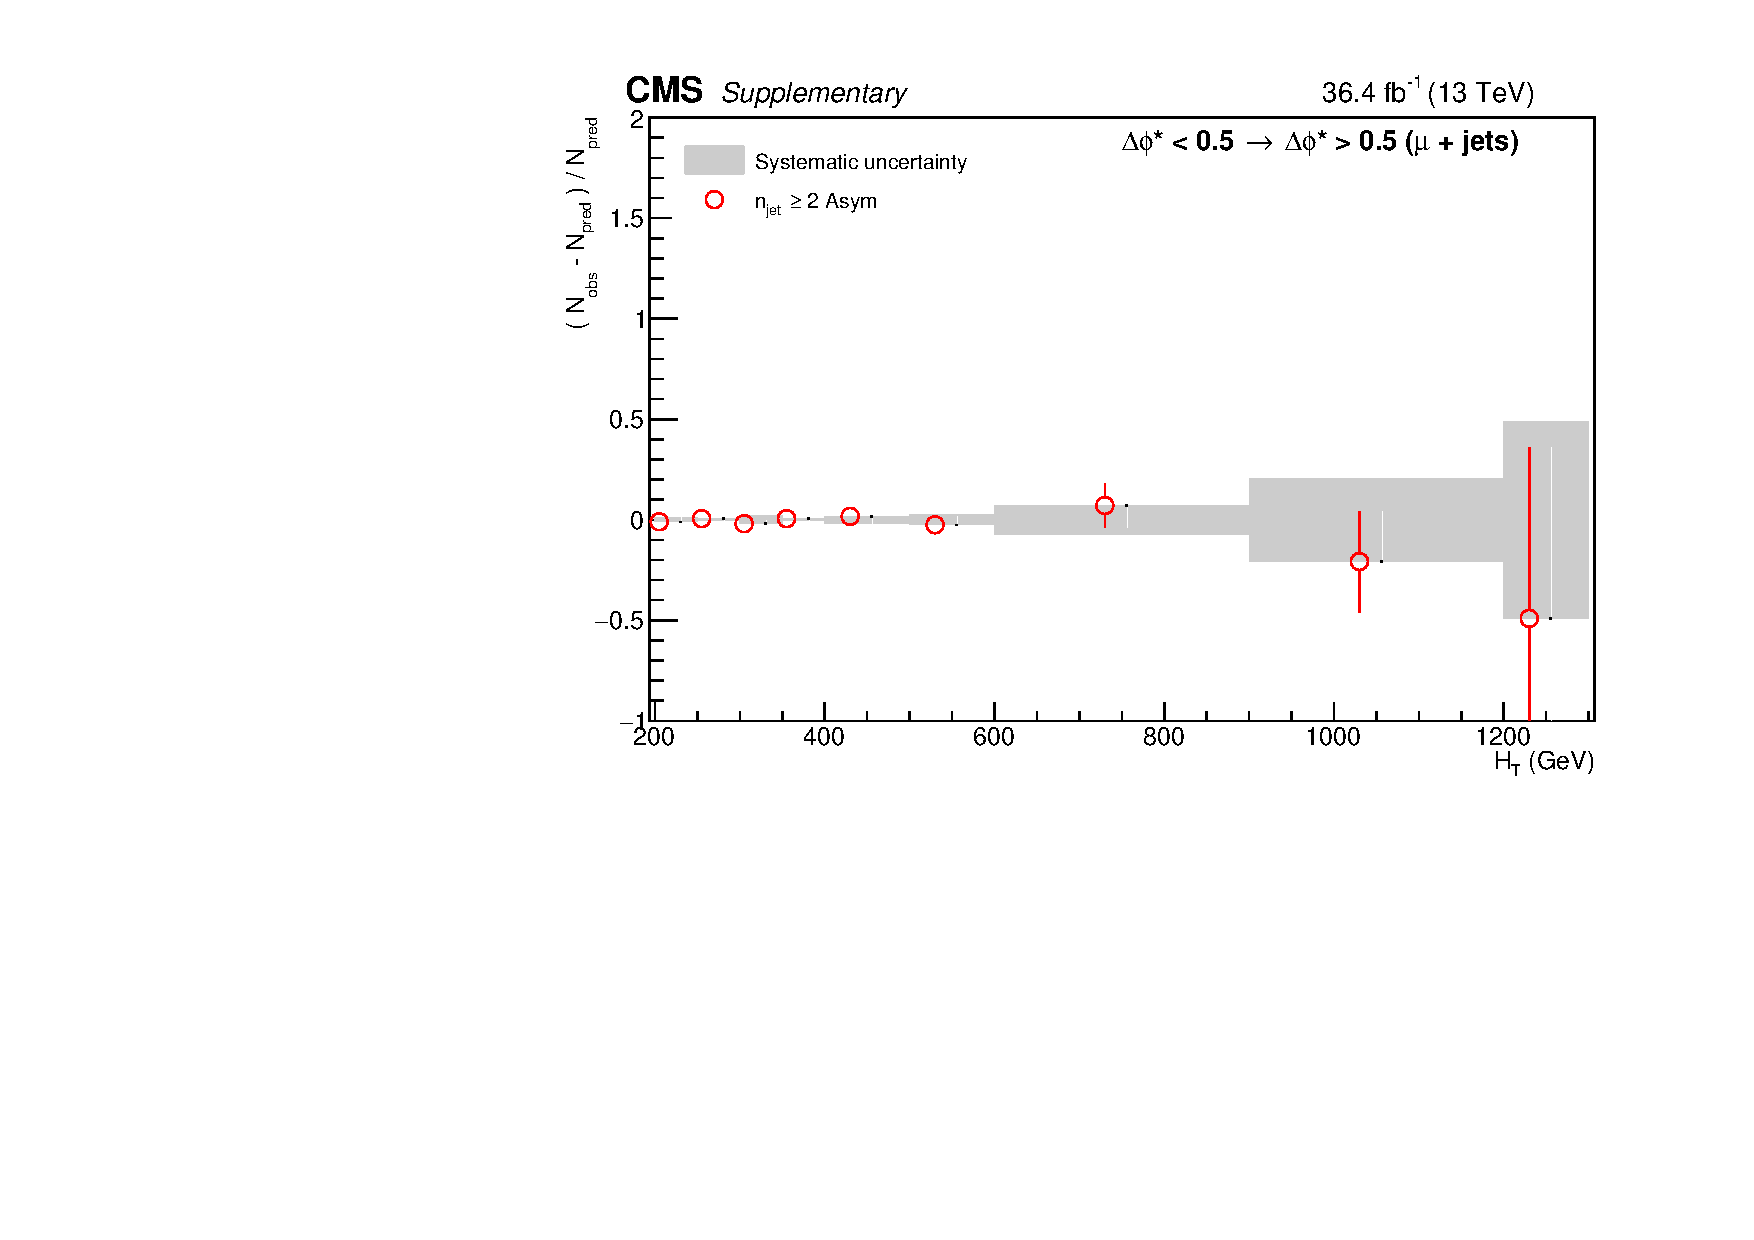
\includegraphics[width=0.5\textwidth]{figures/closureTests/bDPhi_asym__noFit.pdf}} 
    \caption{Data-driven tests probing the \bdphi extrapolation for each
      \njet category (open symbols) overlaid on top of the systematic
      uncertainty estimates used for each \scalht bin (shaded bands). 
      The symmetric (asymmetric) jet topologies are shown in the left (right) plot. 
    }
    \label{fig:closure_bdphi}
  \end{center} 
\end{figure}

\begin{figure}[h!]
  \begin{center}
    \subfigure[]{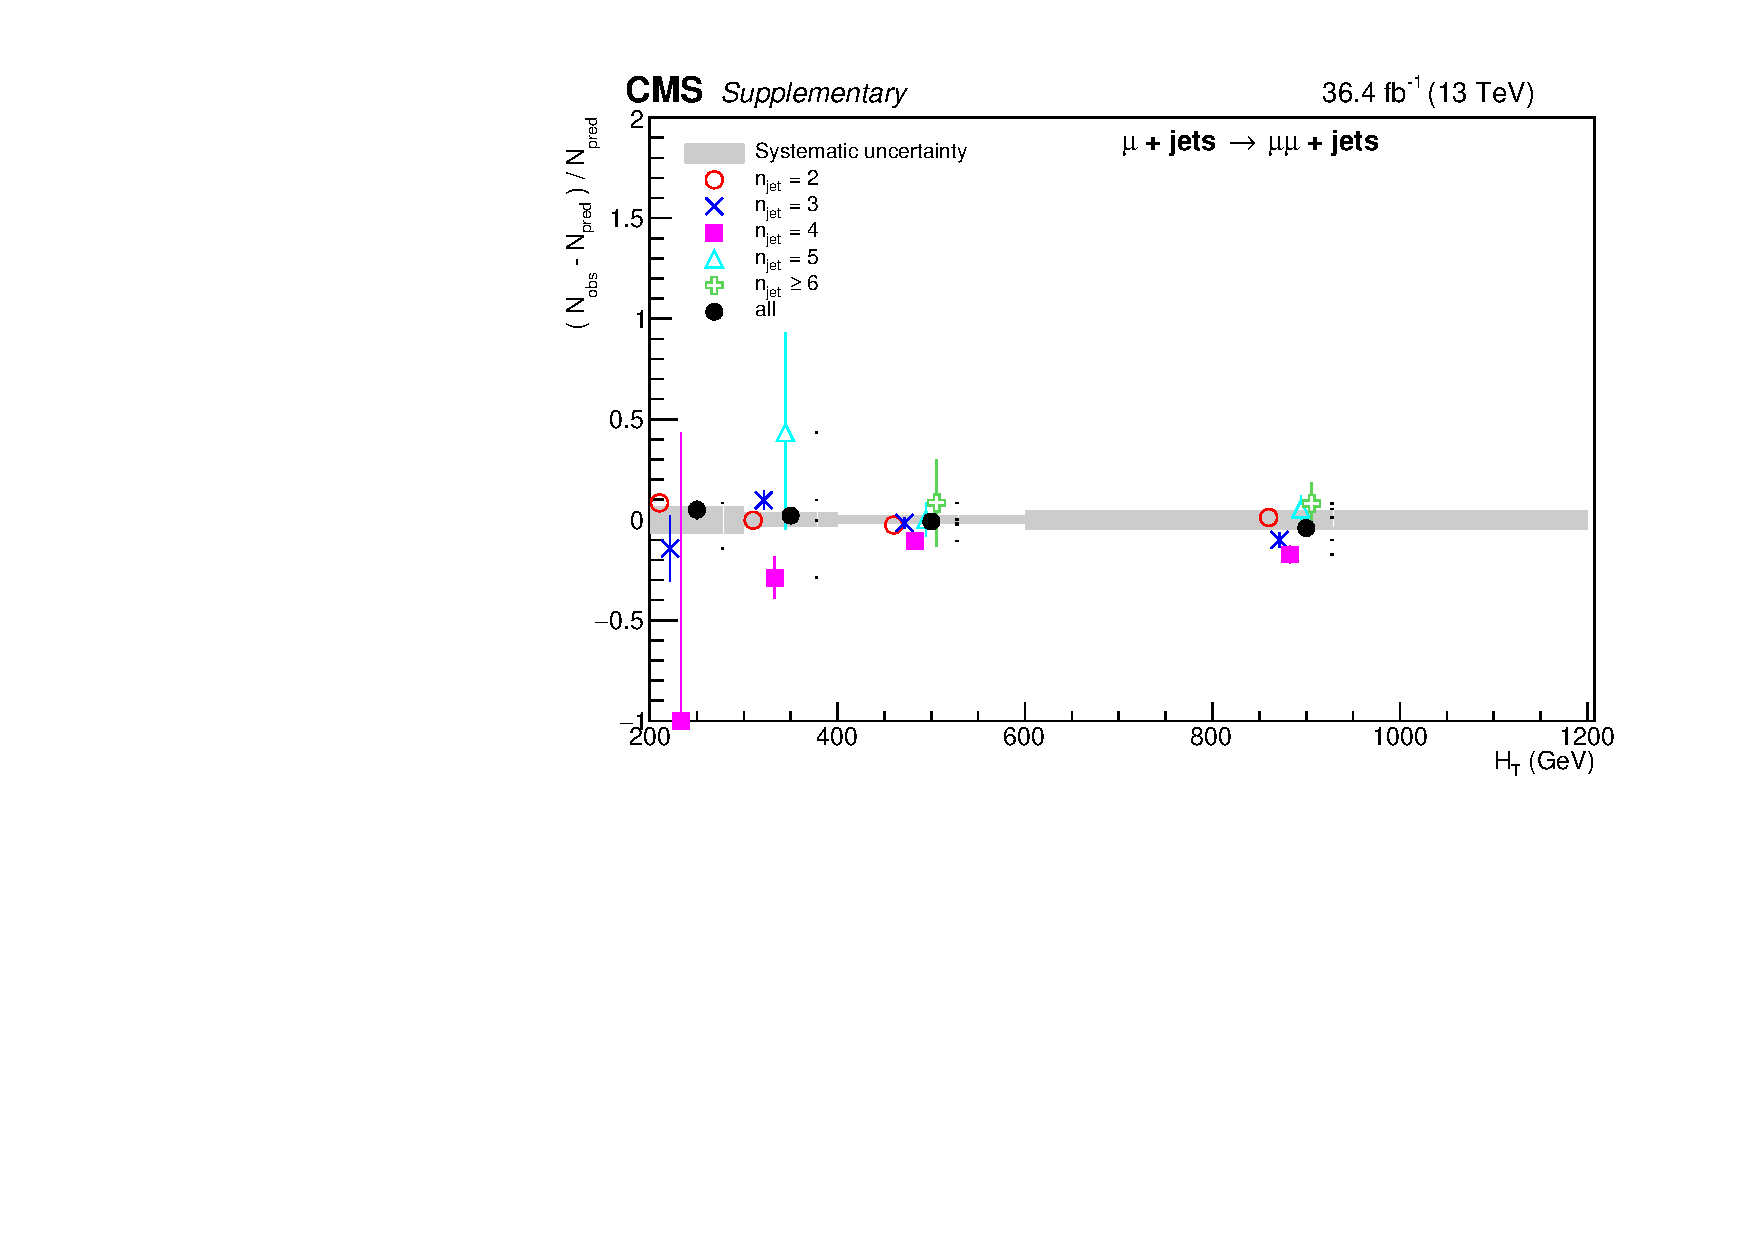
\includegraphics[width=0.5\textwidth]{figures/closureTests/mu_mumu_sym_half_noFit.pdf}}
    ~~
    \subfigure[]{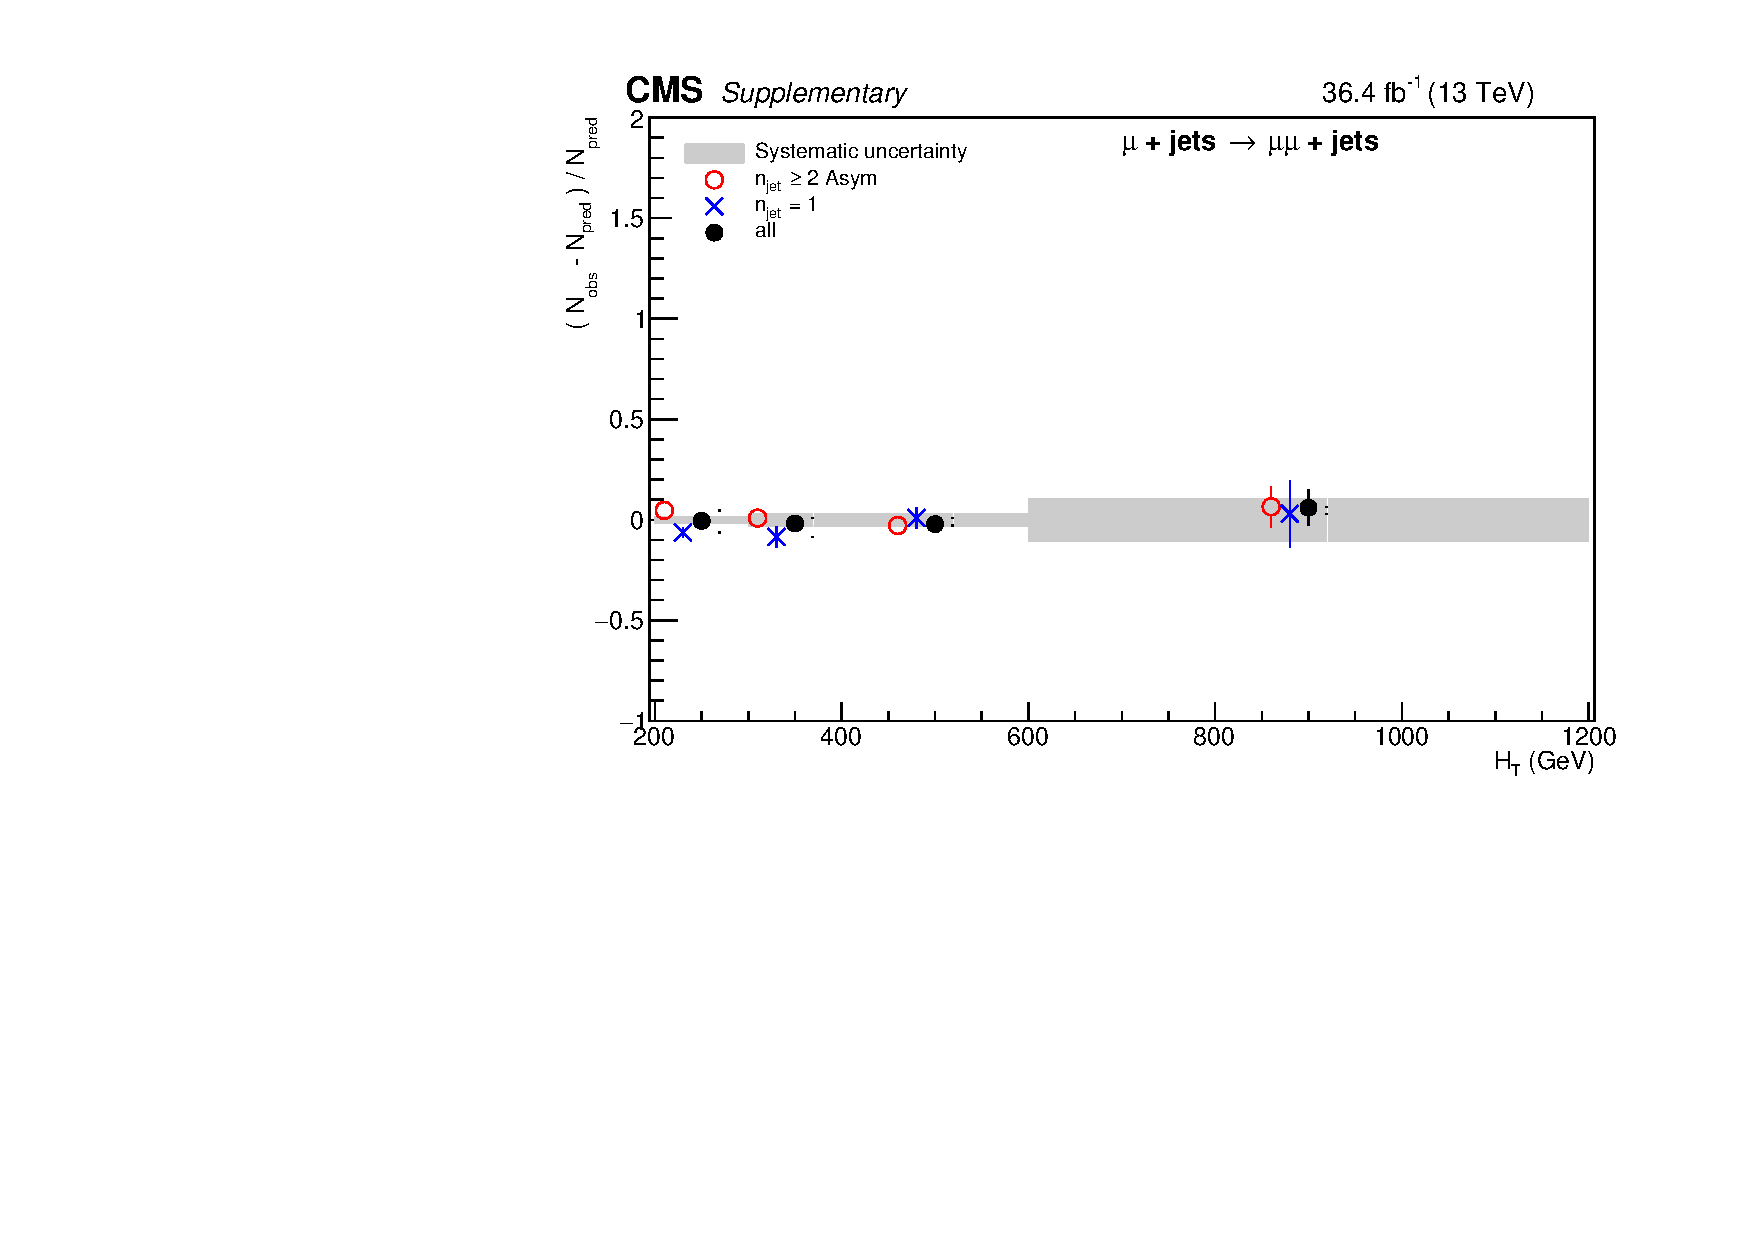
\includegraphics[width=0.5\textwidth]{figures/closureTests/mu_mumu_asym_half_noFit.pdf}} 
    \caption{Data-driven tests probing the use of the \mj control sample
      to predict the \znunu background for each
      \njet category (open symbols) overlaid on top of the systematic
      uncertainty estimates used for each \scalht bin (shaded bands).  
      The symmetric (asymmetric) jet topologies are shown in the left (right) plot. 
    }
    \label{fig:closureMuToMuMu}
  \end{center} 
\end{figure}

\begin{figure}[h!]
  \begin{center}
    \subfigure[]{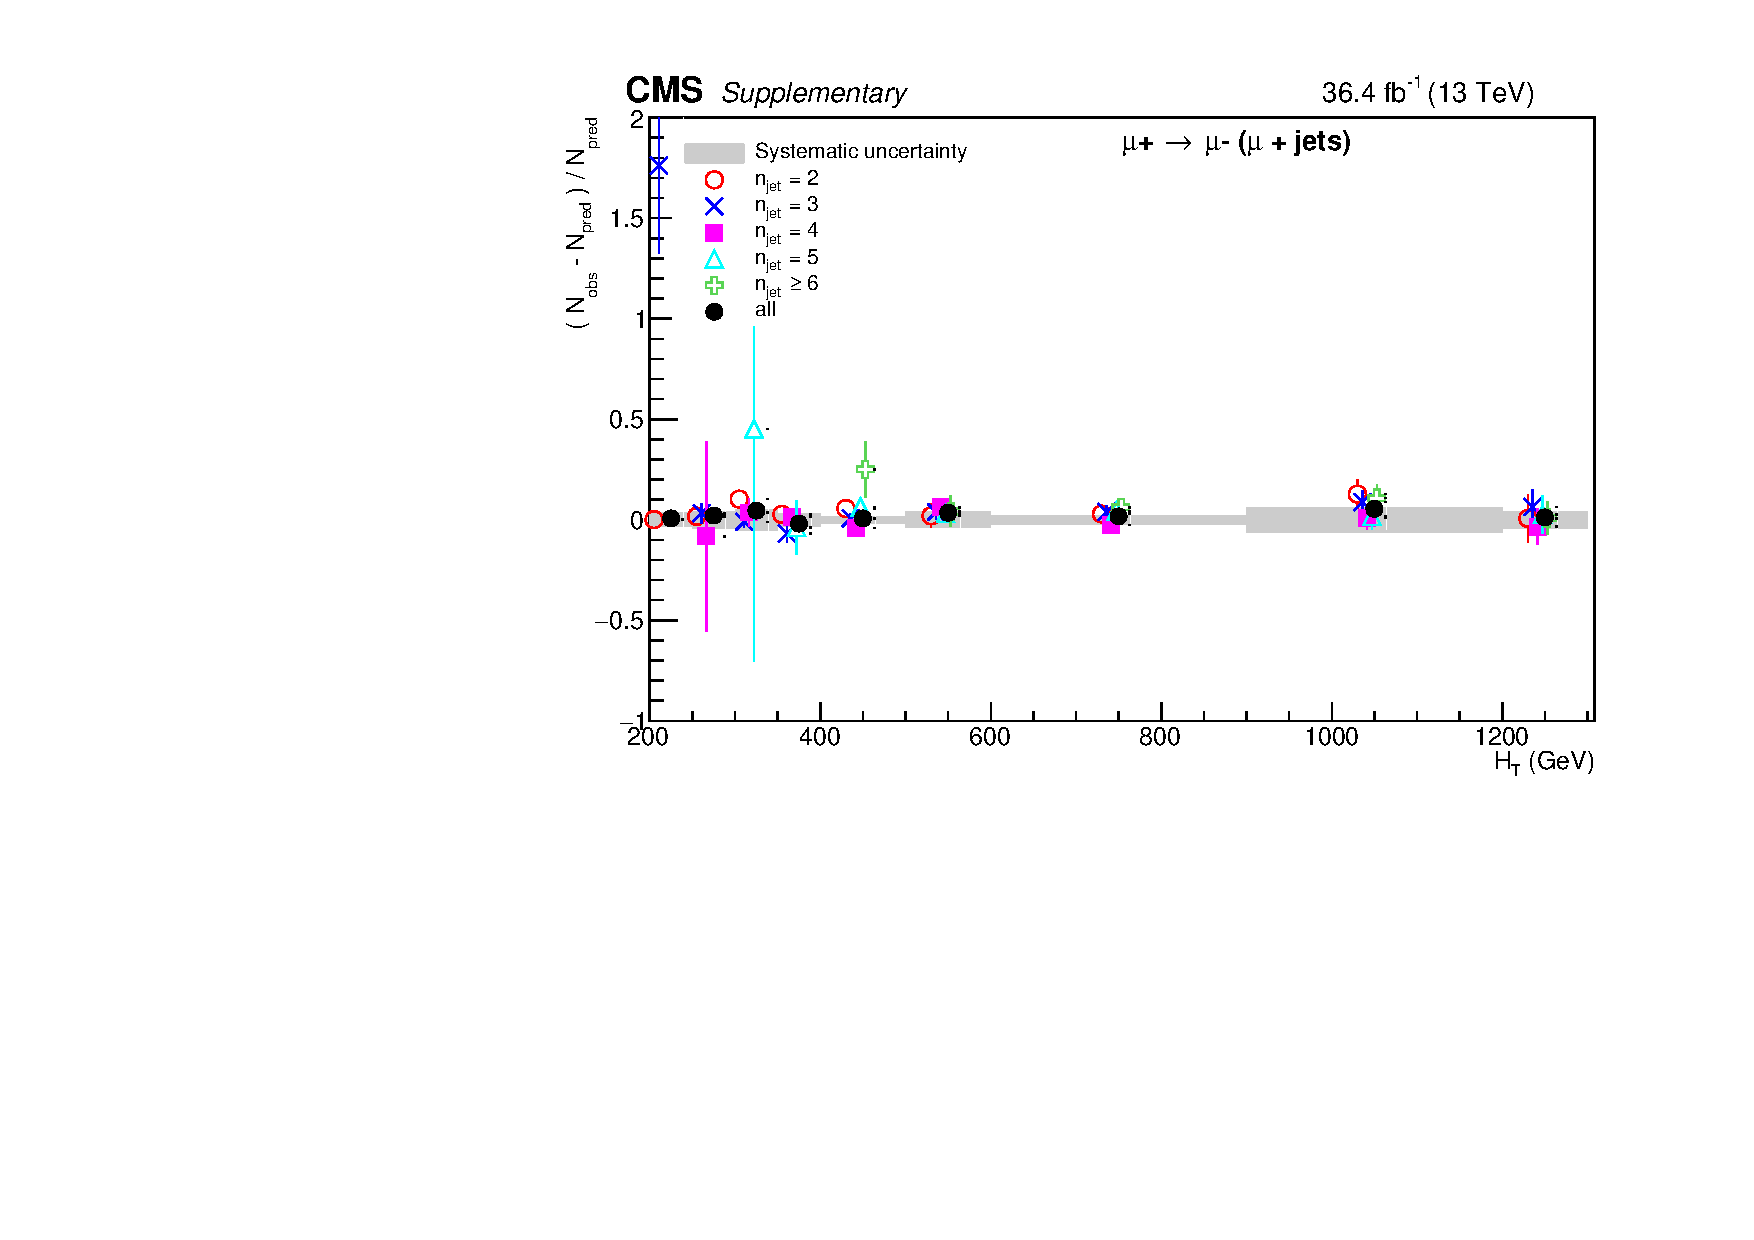
\includegraphics[width=0.5\textwidth]{figures/closureTests/muplus_muminus_sym__noFit.pdf}}
    ~~
    \subfigure[]{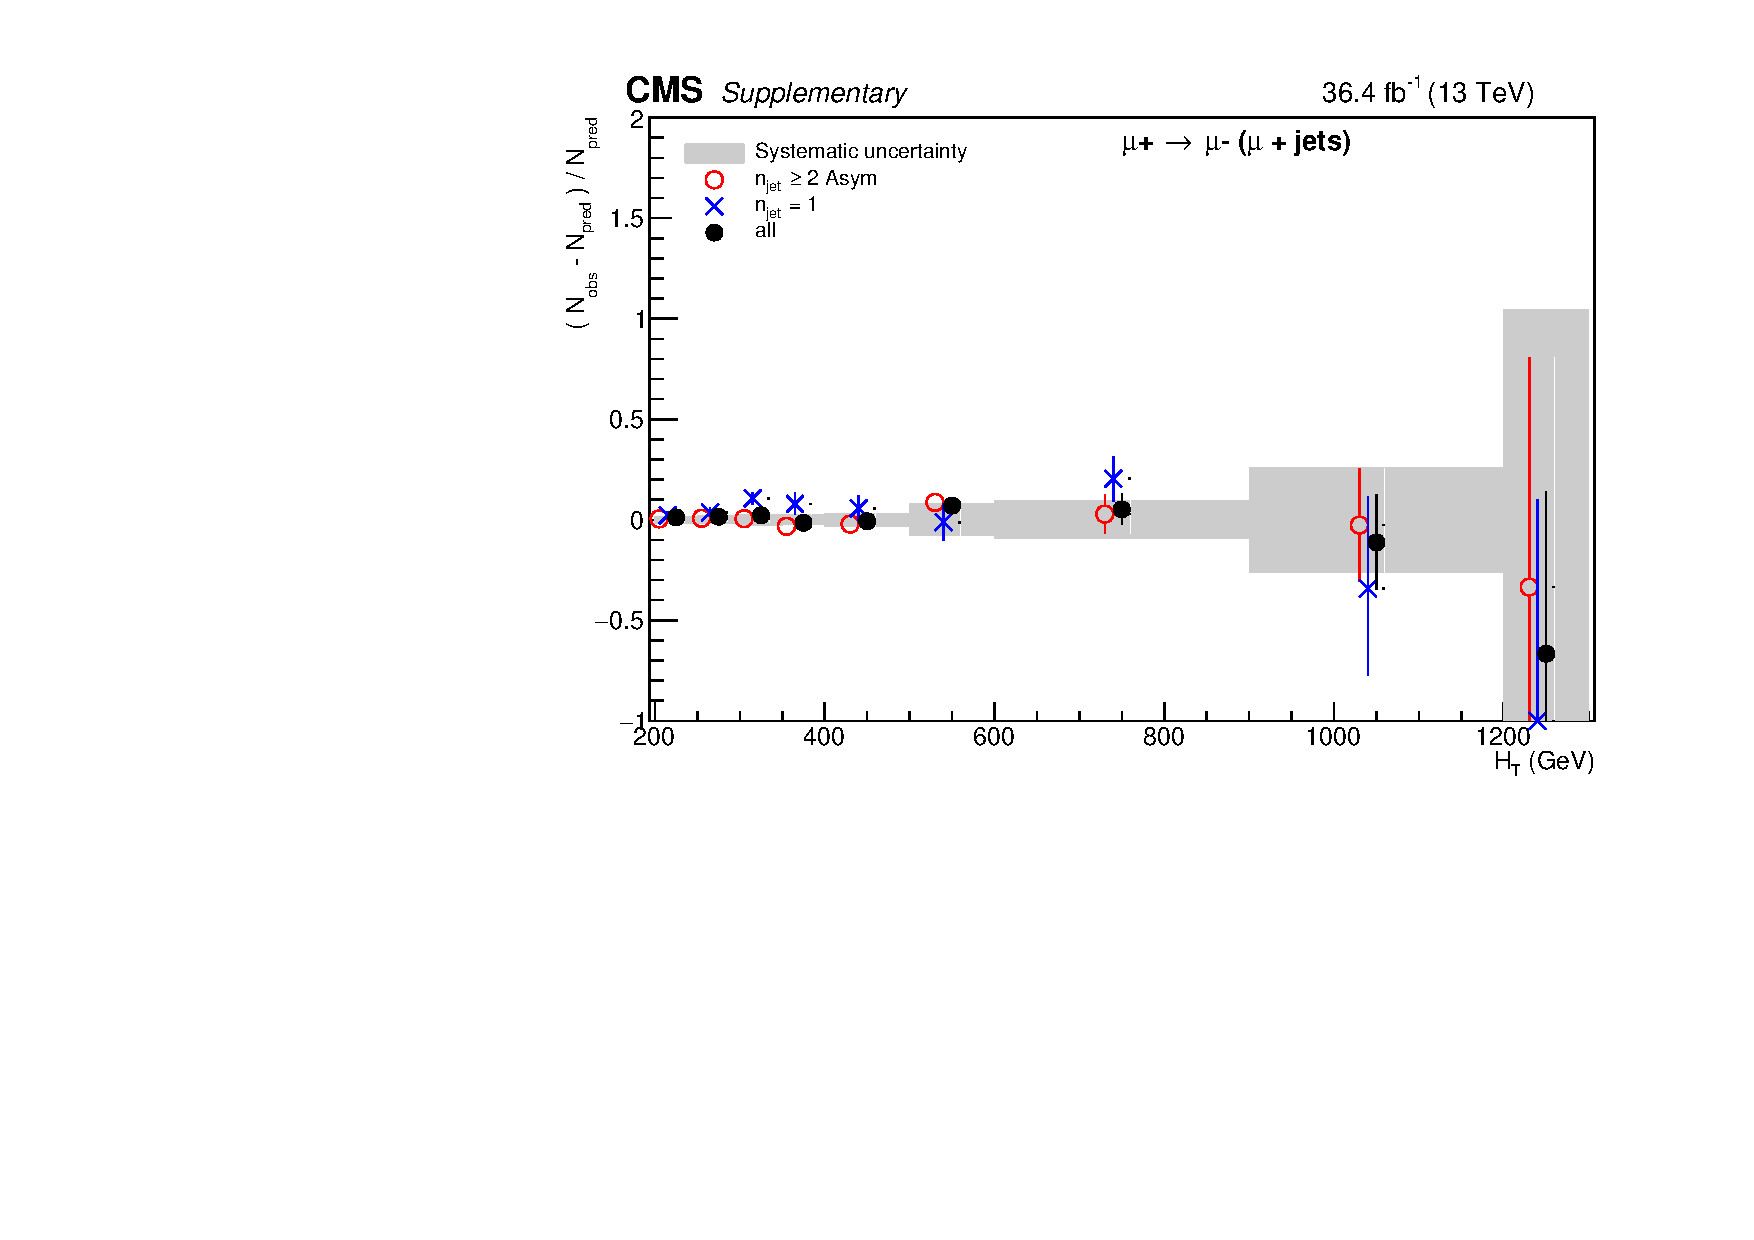
\includegraphics[width=0.5\textwidth]{figures/closureTests/muplus_muminus_asym__noFit.pdf}} 
    \caption{Data-driven tests probing the W polarisation effects. 
      These are shown for each
      \njet category (open symbols) overlaid on top of the systematic
      uncertainty estimates used for each \scalht bin
      (shaded bands). 
      The symmetric (asymmetric) jet topologies are shown in the left (right) plot.       
    }
    \label{fig:closureMuPToMuM}
  \end{center} 
\end{figure}

\begin{figure}[h!]
  \begin{center}
    \subfigure[]{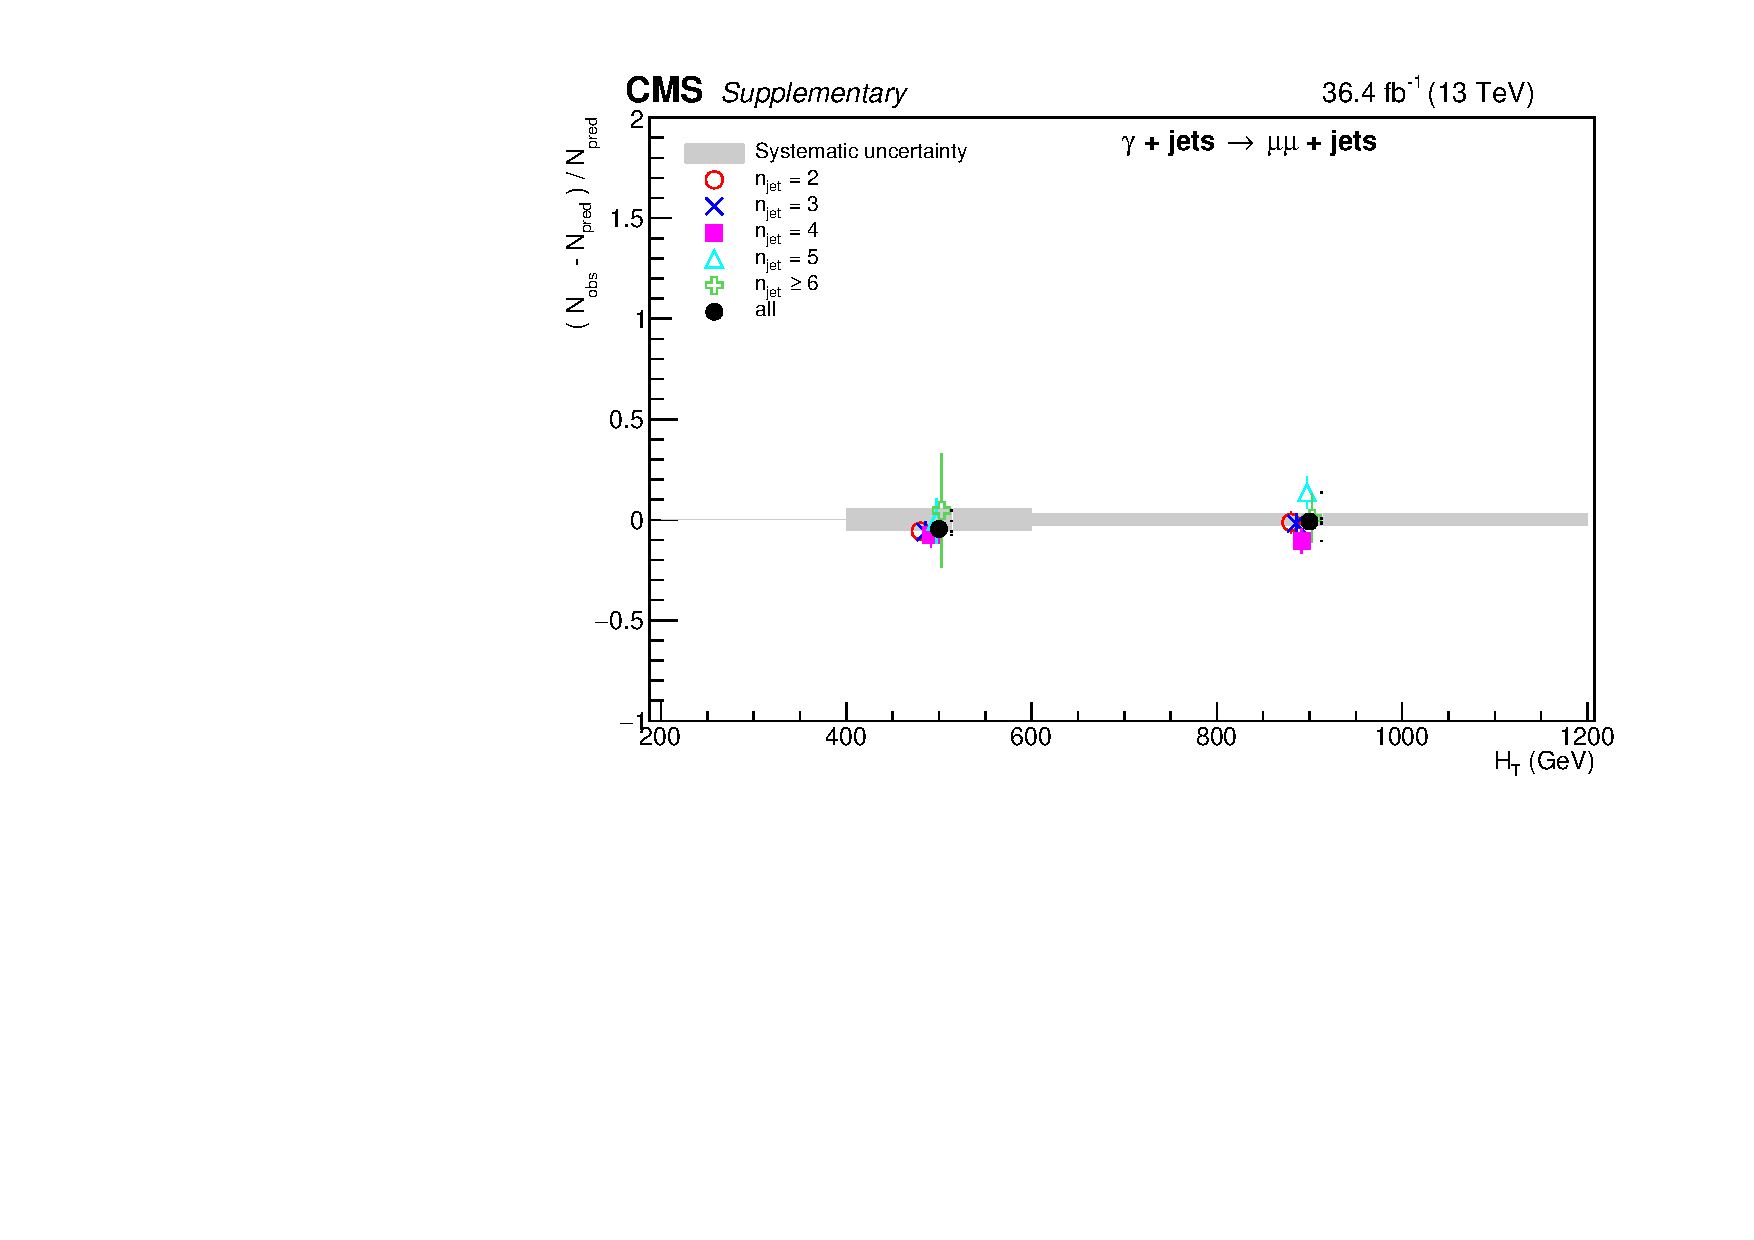
\includegraphics[width=0.5\textwidth]{figures/closureTests/phot_mumu_sym_half_noFit.pdf}}
    ~~
    \subfigure[]{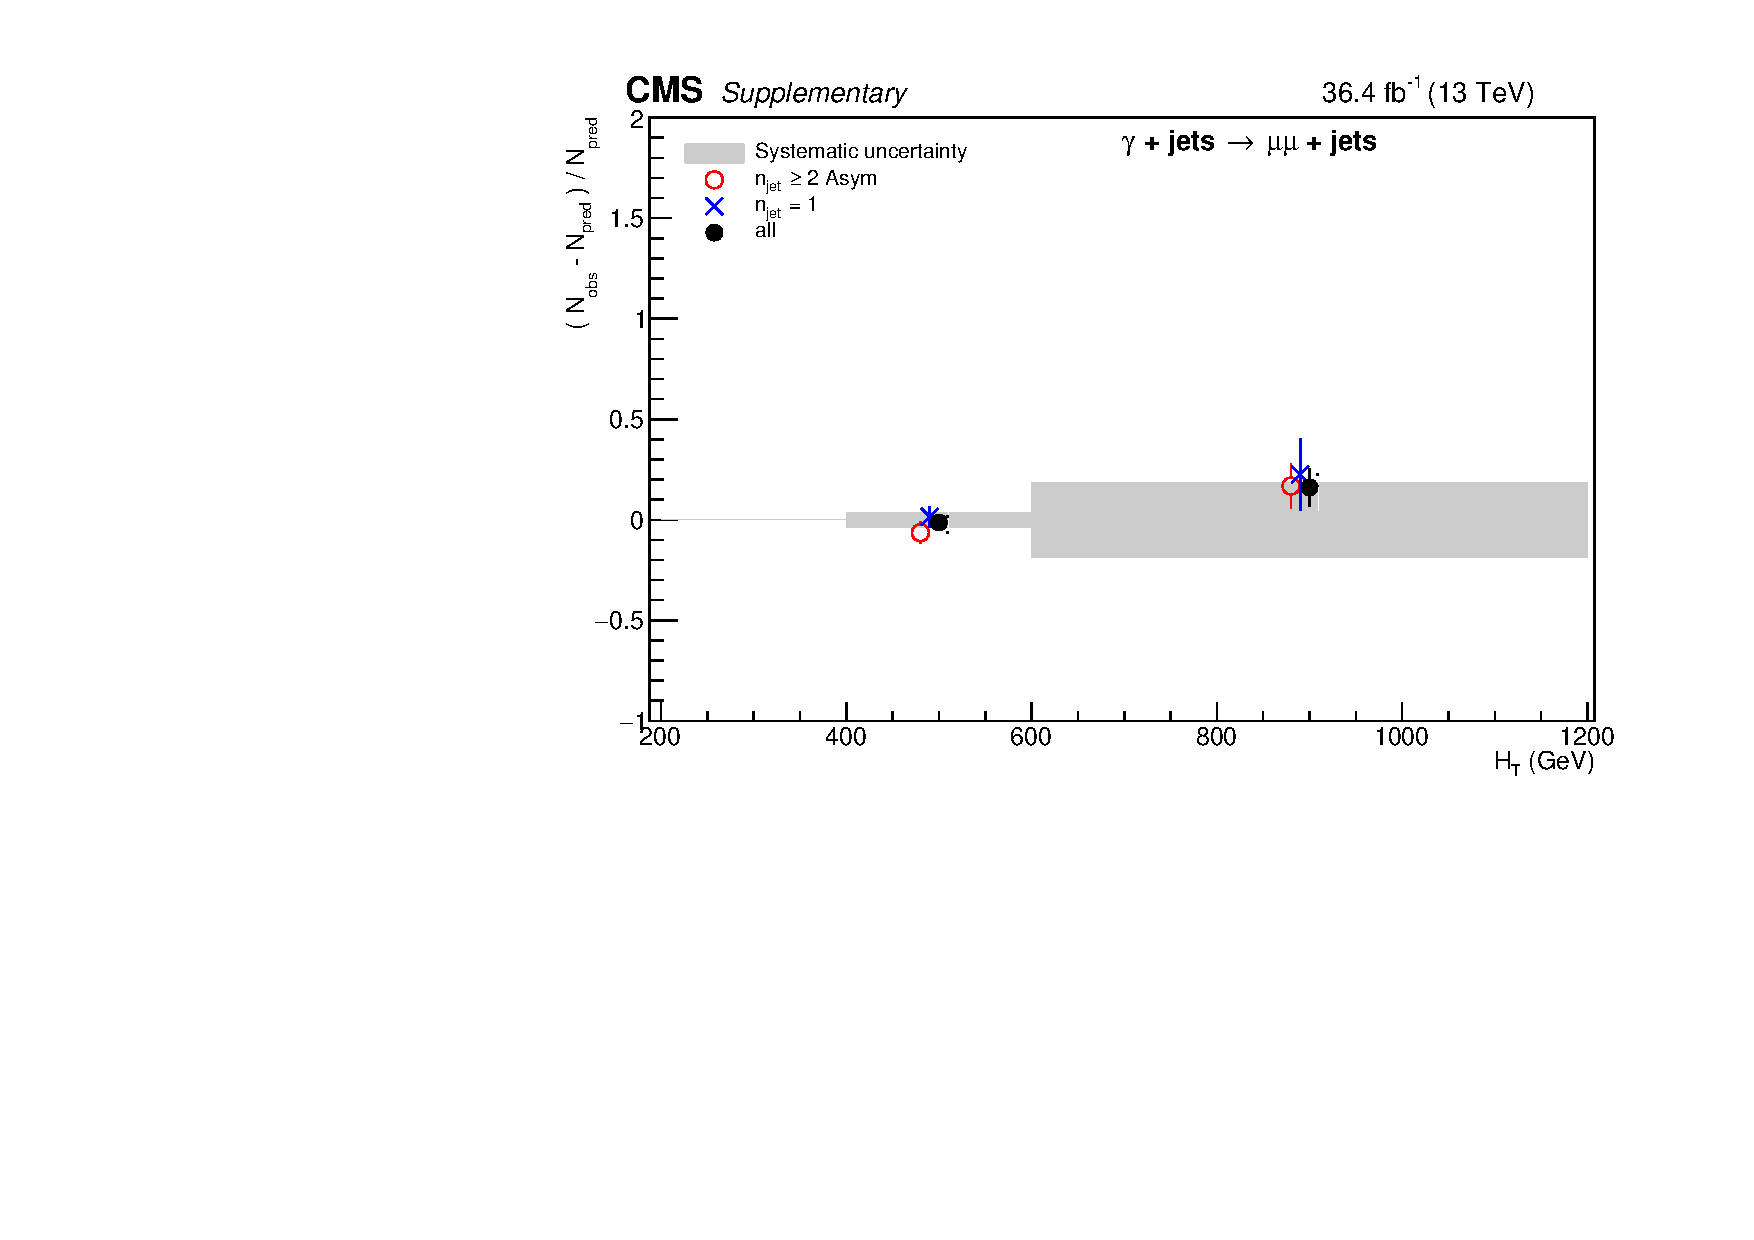
\includegraphics[width=0.5\textwidth]{figures/closureTests/phot_mumu_asym_half_noFit.pdf}} 
    \caption{Data-driven tests probing the Z/$\gamma$ ratio for each
      \njet category (open symbols) overlaid on top of the systematic
      uncertainty estimates used for each \scalht bin
      (shaded bands). 
      The symmetric (asymmetric) jet topologies are shown in the left (right) plot.      
    }
    \label{fig:closurePhoToMuMu}
  \end{center} 
\end{figure}

\begin{figure}[h!]
  \begin{center}
    \subfigure[]{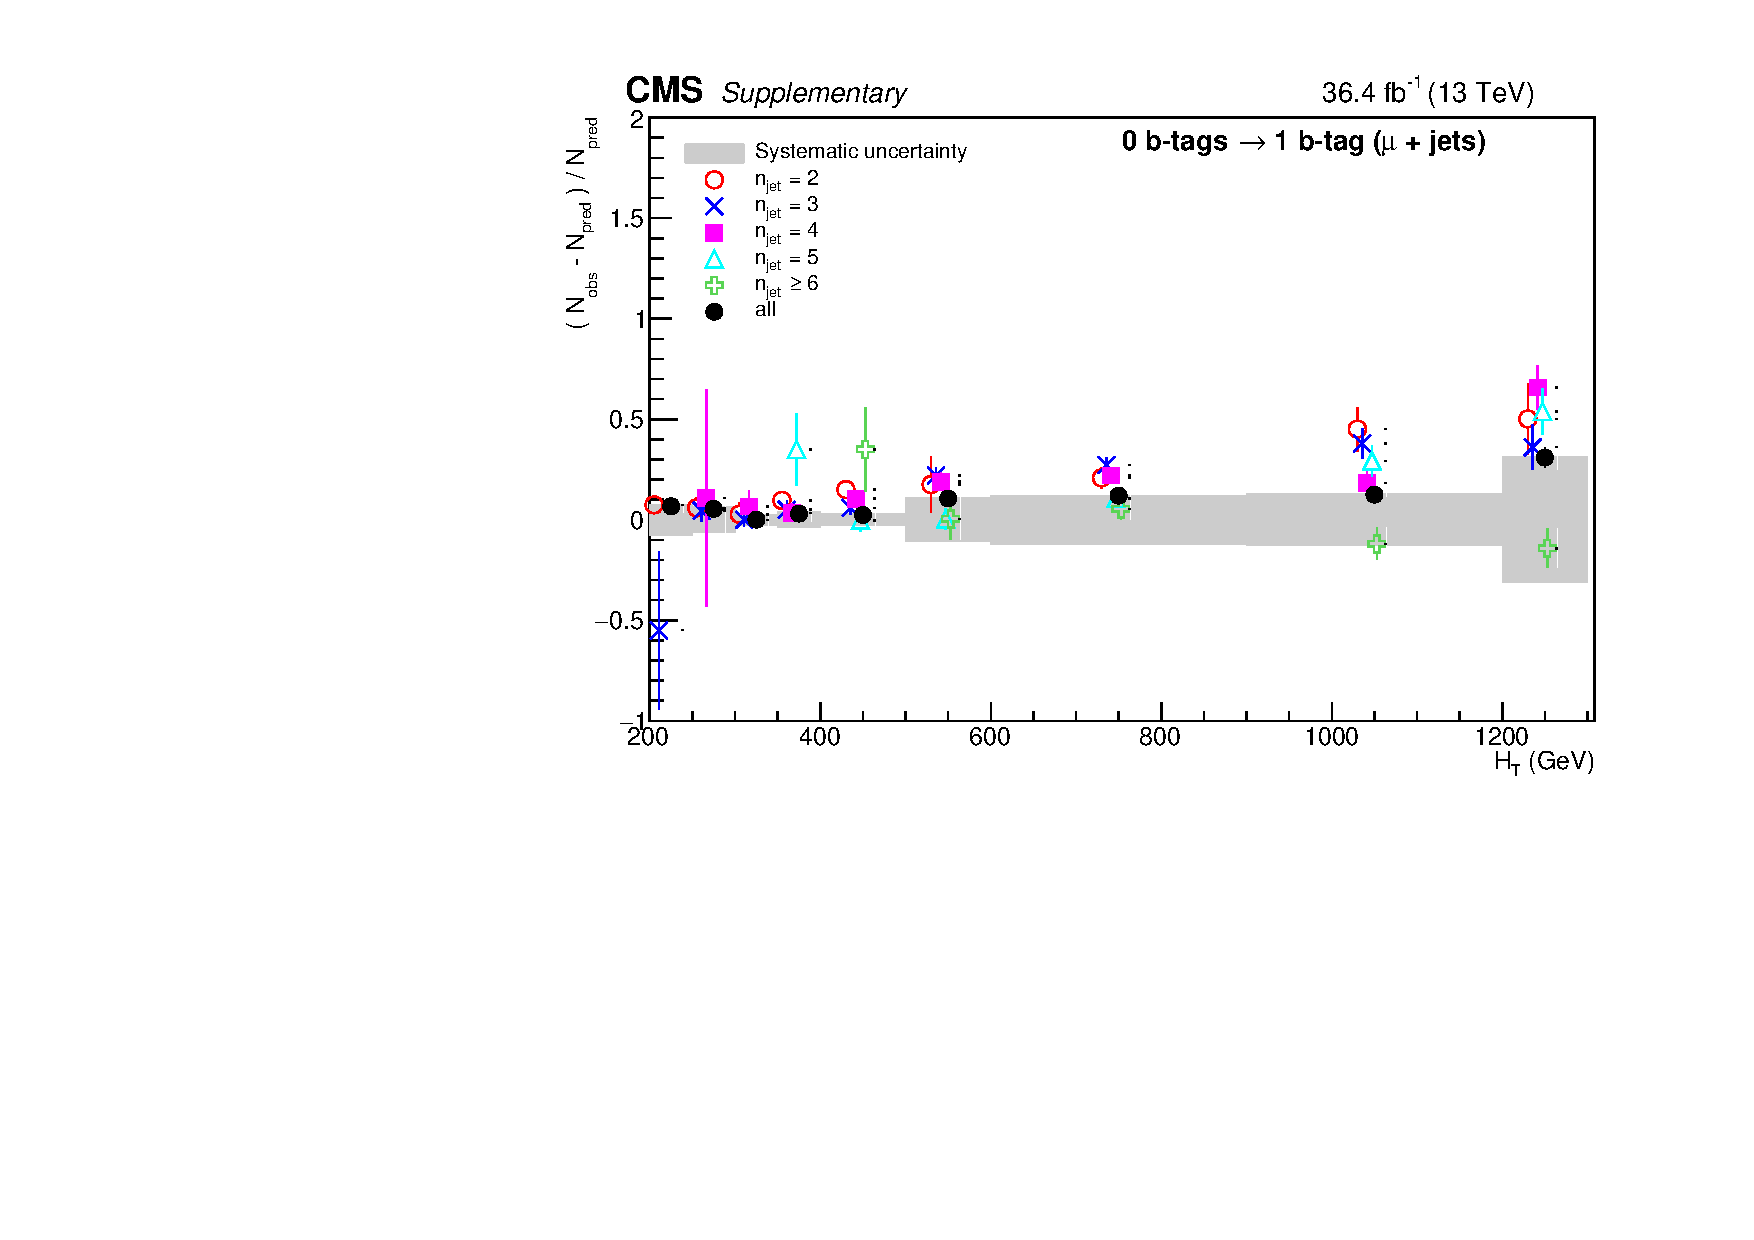
\includegraphics[width=0.5\textwidth]{figures/closureTests/eq0b_eq1b_muon_sym__noFit.pdf}}
    ~~
    \subfigure[]{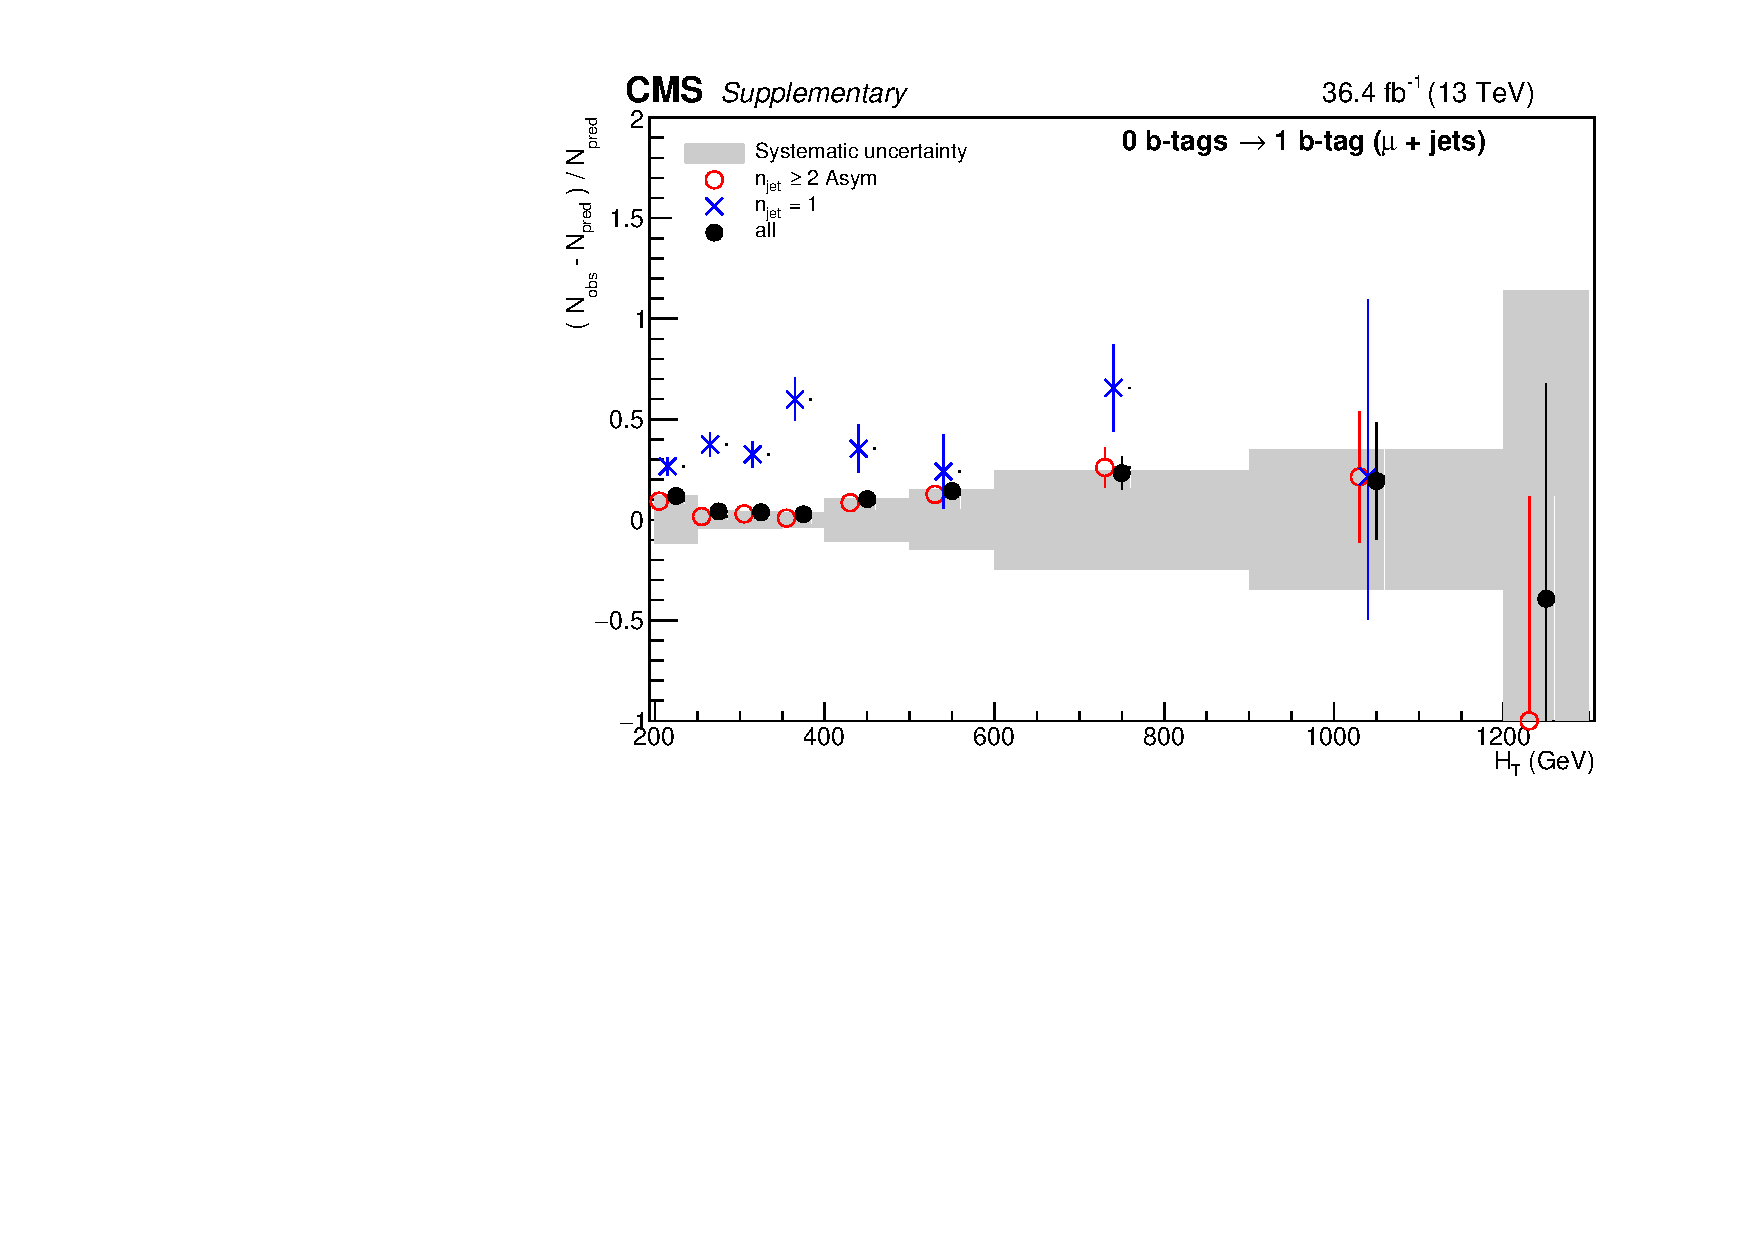
\includegraphics[width=0.5\textwidth]{figures/closureTests/eq0b_eq1b_muon_asym__noFit.pdf}} 
    \caption{Data-driven tests probing the W and \ttbar admixture in
      each \njet category (open symbols). The symmetric (asymmetric)
      jet topologies are shown in the left (right) plot. The BTV POG
      b-tag SFs and their uncertainties are applied in the analysis,
      discussed in Section~\ref{sec:inputs-and-updates}, thus the
      derived systematic is not propagated to the fit. Instead this 
      closure tests is inspected solely as a cross-check. 
    }
    \label{fig:closureBTag}
  \end{center} 
\end{figure}

\newpage
\begin{landscape}
\begin{table}[h!]
  \caption{Summary of the systematics on the transfer factors considered in the analysis, 
    with representatives ranges of uncertainties and the correlation assumed, 
    for the predictions of the $\ttbar$, W and $\znunu$  background
    components.}
  \label{tab:systs}
  \centering
  \scriptsize
  \begin{tabular}{ ccccccc }
    \hline
    \hline
    Systematic & Method & \multicolumn{4}{c}{Relative uncertainty on transfer factor} & Correlation model \\    
    & & $\mj \rightarrow \znunu$  & $\mmj \rightarrow \znunu$ & $\gj \rightarrow \znunu$ & $\mj \rightarrow \ttbar+W$ & \\
    \hline
    Jet energy scale                  & MC variations     & $1-5\%$  & $1-5\%$  & $1-5\%$  & $1-5\%$  & fully correlated                      \\
    B-tagging efficiency b and c jets & MC variations     & $1-3\%$  & $1-3\%$  & $1-3\%$  & $1-3\%$  & fully correlated                      \\
    B-tagging efficiency light jets   & MC variations     & $1-3\%$  & $1-3\%$  & $1-3\%$  & $1-3\%$  & fully correlated                      \\
    Pileup weights                    & MC variations     & $1-7\%$  & $1-7\%$  & $1-7\%$  & $1-7\%$  & fully correlated                      \\
    %Top $p_{T}$ weights              & MC variations     & $1-30\%$ & $1-10\%$ & -        & $1-10\%$ & fully correlated                      \\
    Lepton scale factor               & MC variations     & $1-3\%$  & $1-3\%$  & -        & $1-3\%$  & fully correlated                      \\
    Signal trigger efficiency         & MC variations     & $1-7\%$  & $1-7\%$  & $1-7\%$  & $1-7\%$  & fully correlated                      \\
    %Photon trigger efficiency        & MC variations     & -        & -        & $1-2\%$  & -        & fully correlated                      \\
    \hline
    \alphat/\bdphi extrapolation      & data-driven tests & $3-20\%$ & $3-20\%$ & -        & $3-20\%$ & un-correlated across \scalht/jet top. \\
    W/Z ratio                         & data-driven tests & $1-12\%$ & -        & -        & -        & un-correlated across \scalht/jet top. \\
    Z/$\gamma$ ratio                  & data-driven tests & -        & -        & $2-26\%$ & -        & un-correlated across \scalht/jet top. \\
    W polarisation                    & data-driven tests & $2-14\%$ & -        & -        & $2-14\%$ & un-correlated across \scalht/jet top. \\
    \hline
    \hline
  \end{tabular}
\end{table}

\end{landscape}

%%%____________________________________________________________________________||
\section{Systematic uncertainties in the \mht dimension}
\label{sec:syst-on-shape}

The estimate of the number of events per (\njet,~\nb,~\scalht) bin,
integrated over \mht, is derived from data control samples, with
the associated systematic uncertainty determined as 
described in Sec.~\ref{sec:closure-tests}. This section
describes the method used to assess the systematic uncertainties in
the distribution of events according to \mht. A data driven approach is
utilised under the hypothesis of zero bias in the data and MC agreement.
The level of closure in the control regions is used
to derive alternative templates accounting for systematic uncertainties.
It is important to note that the data-driven systematics on the 
\mht distribution are included in addition to known uncertainties.

When looking at the \mht dimension inclusively in \scalht there are
large theoretical uncertainties that originate from mixing events
at different scales. These uncertainties can be mitigated if the events 
are binned according to a variable, such as \scalht, 
which is strongly correlated with the scale of the event. 
After this categorisation is applied, the uncertainty in 
the distribution of the \mht variable
(as well as any other MET-like variable) is expected to be 
mainly affected by the MC modelling of the particle 
decays and, to a lesser extent, by jet reconstruction effects, 
such as jet energy scale and resolution. 
This approach, which will be often referred to as \textit{scale anchoring}
in the following, is used in this analysis. The distribution in \mht
is measured in data using the control regions and compared to MC
to determine the validity of the zero bias hypothesis after scale anchoring.

In Sec.~\ref{sec:valid13} the 13 \TeV data is used used 
to validate the scale anchoring approach. 
In Sec.~\ref{sec:systMhtDimension} 
the procedure used to extract the systematic uncertainties in the 
\mht dimension is described and results shown with 13 \TeV data. 
% In Appendix~\ref{sec:bias_injection} the results of a bias injection test described. 
% This shows that the fit is sensitive to a bias affecting only the last \mht bin.
%% Finally, in Sec.~\ref{app:closureTests3fb} the expected systematics for 3\ifb in Run 2 are be shown. 


% extent to which the control regions can constrain this bias 
% to the flat hypothesis
%Motivated by the inclusive distribution, a linear bias is assumed.

\subsection{Validation with 13 TeV Data}
\label{sec:valid13}
In previous versions of this analysis three control regions
were used: \mj, \mmj and \gj. To parameterise the data/MC agreement
orthogonal polynomials are used such that odd and even powers 
are decorrelated \cite{cohen2013applied}. 
The $n^{th}$ order orthogonal polynomial which is fitted to the data/MC 
distribution is defined in Eq.~\ref{equ:orthog-polynomial}.

\begin{equation}
  \label{equ:orthog-polynomial}
  f_n(x) = \sum_{k=0}^{k=n}{(p_k)\times(\bar{x}-x)^k}
\end{equation}

where $\bar{x}$ is the weighted mean of the distribution and $p_k = 0$ 
implies the $k^{th}$ order term is negligible.
In Fig.~\ref{fig:linearMotiv} the data/MC 
distribution against \mht for the control region selection 
(detailed in \cite{Khachatryan:2016pxa}) is shown inclusive 
in \scalht and categories. By fitting a first order
orthogonal polynomial it can be seen that there is a large bias. 
This bias in the data/MC agreement is expected as events 
at different scales are mixed.
The first order orthogonal polynomial
is used to measure the level of bias remaining 
when the \mht dimension is binned in \scalht.
This allows the normalisation parameter to be
decorrelated from the parameter which controls
the distribution in \mht.
The normalisation in each \scalht bin and its systematics 
is then defined following the data-driven method used in Run 1, see Sec,~\ref{sec:systMhtDimension} for details.
\begin{figure}[h!]
  \centering
  \subfigure[\mj]{
    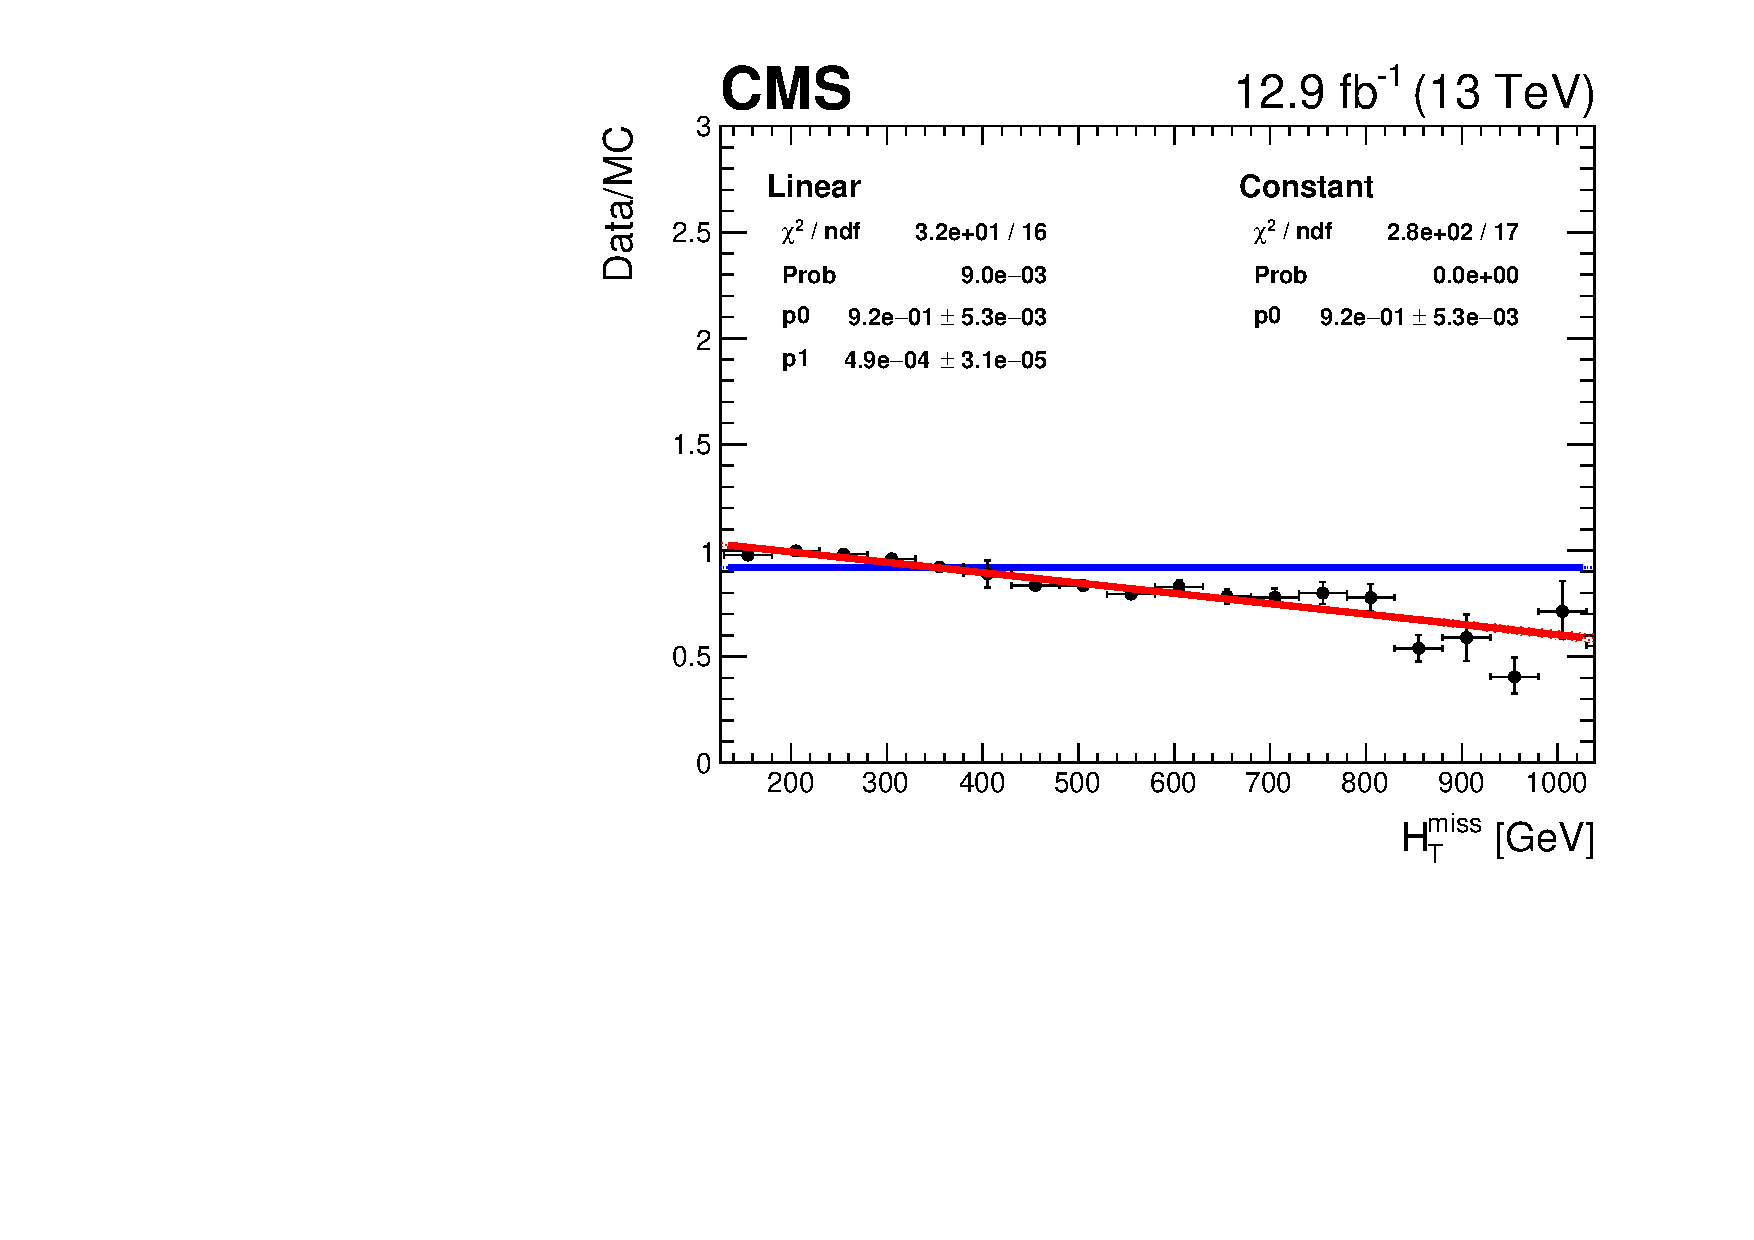
\includegraphics[width=0.5\textwidth]{figures/mhtTemplate/inclusive/mht_Inc_Inc_ht_Inc_SingleMu_Graph.pdf}
  }~~
  \subfigure[\gj]{
    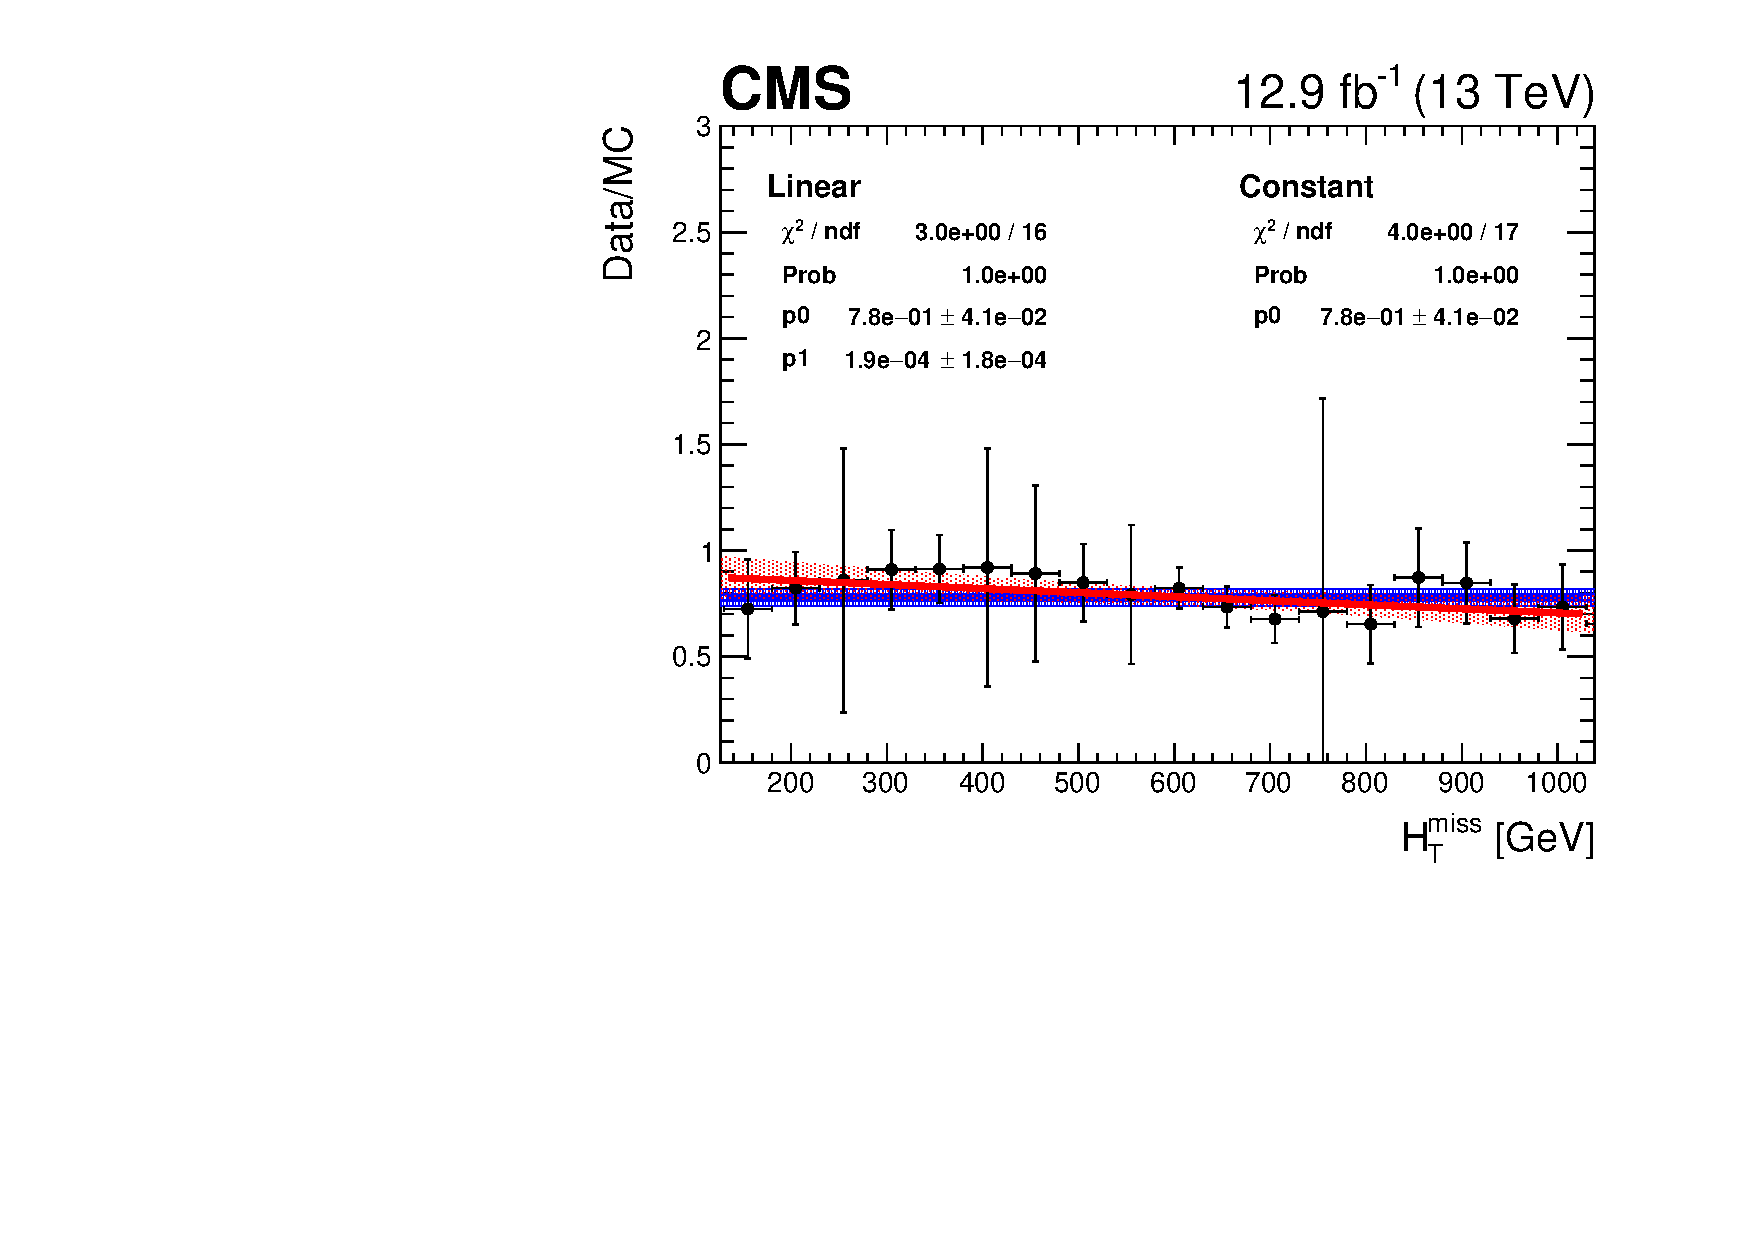
\includegraphics[width=0.5\textwidth]{figures/mhtTemplate/inclusive/mht_Inc_Inc_ht_Inc_SinglePhoton_Graph.pdf}
  }\\
  \subfigure[\mmj]{
    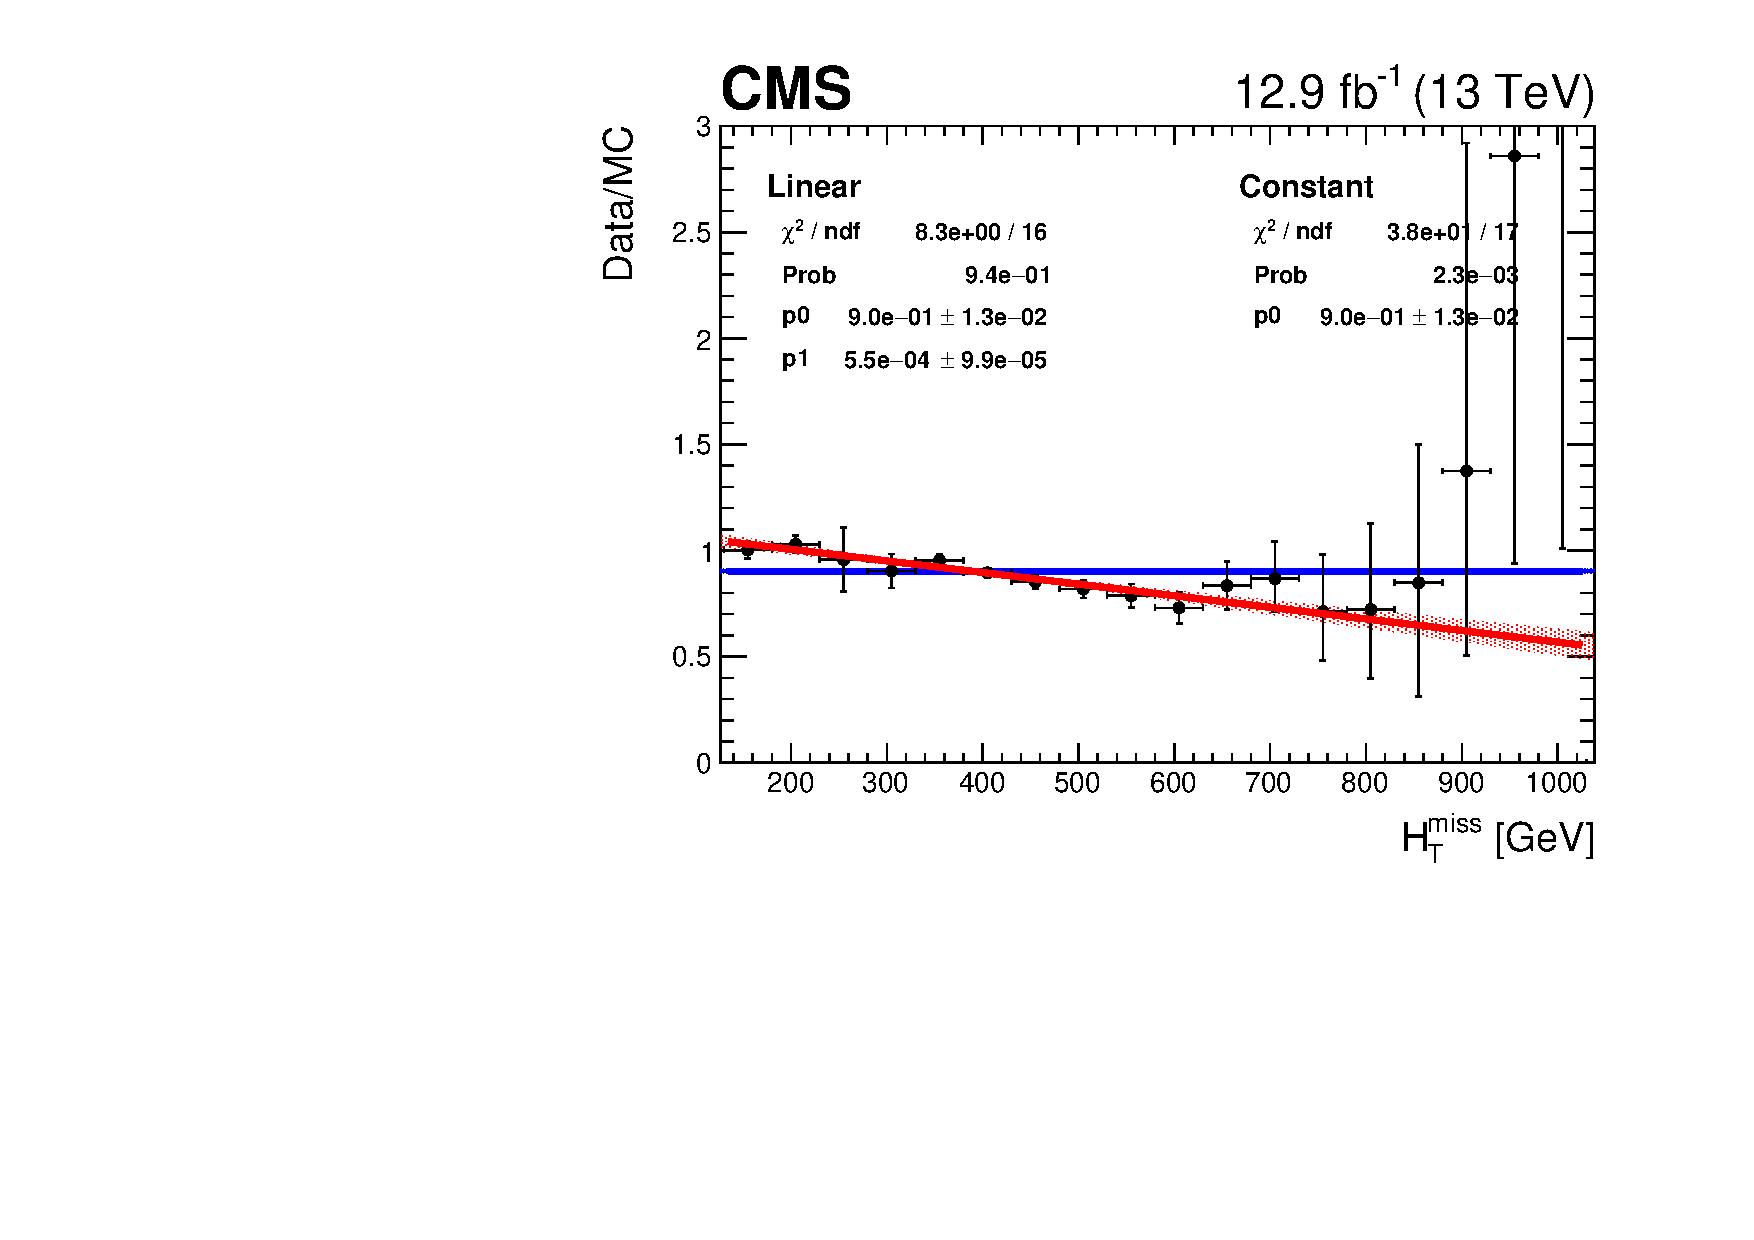
\includegraphics[width=0.5\textwidth]{figures/mhtTemplate/inclusive/mht_Inc_Inc_ht_Inc_DoubleMu_Graph.pdf}
  }\\
  \caption{\label{fig:linearMotiv} 
  The data/MC distribution against \mht for an inclusive selection on category and \scalht
  showing the results of a linear fit. A large bias is observed as well as a low pValue for the constant fits. 
 }
\end{figure}

By anchoring the scale using binning in the \scalht dimension the remaining
bias is assumed to be negligible. In Fig.~\ref{fig:linearFitExamples} 
example fits of an orthogonal linear function to the data/MC ratio 
are shown for the three control regions. Comparing to the inclusive distribution 
the linear component can be seen to be compatible with the null hypothesis, 
i.e. no bias. In order to formalise this assertion 
the pull of the linear component from zero is calculated.
This pull distribution is shown for each of the three control regions in
in Fig.~\ref{fig:pulls}. For the \mmj and \gj samples the mean is consistent 
with zero implying no overall bias. The \mj sample shows some evidence for a small
bias of around 0.3 sigma. Section~\ref{sec:systMhtDimension} details how this bias
is covered in the signal region. All three samples have a sigma consistent with one.
Fig.~\ref{fig:frenchFlagPulls} shows the distribution of the pulls 
in category and \scalht bins showing the pulls are randomly spread across
the categories.


% The linear fits to the data/MC ratio additionally show a p-value following 
% a uniform distribution between 0 and 1 as shown in Fig.~\ref{fig:pValues}.
% This confirms that the linear component is reasonably compatible with zero ($p_1 = 0$), %i.e. no significant bias is observed, 

%Finally, an additional validation 
%can be seen from the p-value distribution of the constant fits
% -- should add p value of constant fit but currently not flat due to
% non guassian behaviour.

\begin{figure}[h!]
  \centering
  \subfigure[\gj, 0b, 5j category and \scalht 750-900\GeV bin]{
    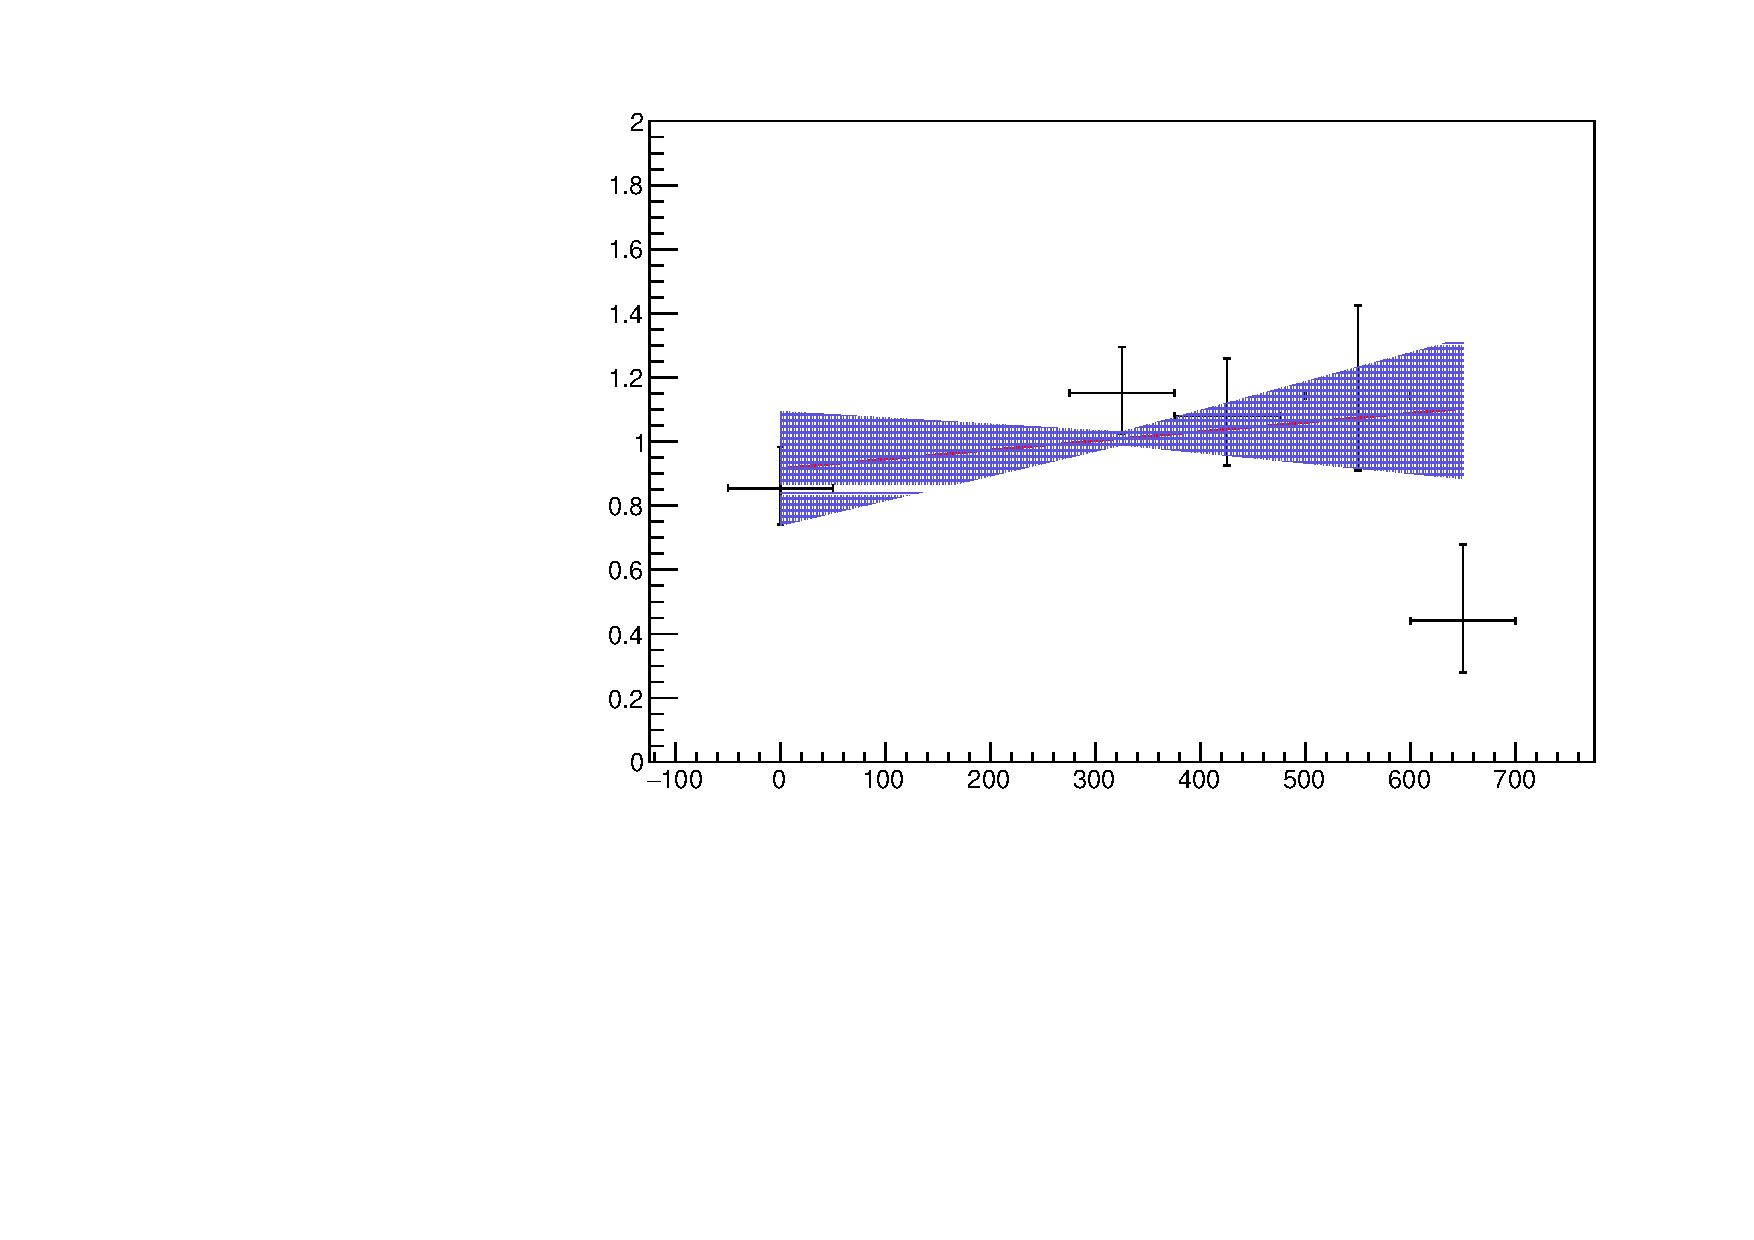
\includegraphics[width=0.5\textwidth]{figures/mhtTemplate/examples/Pho/ht750_900_control_eq0b_eq5j_Pho.pdf}
  }~~
  \subfigure[\mj, 0b, 4j category and \scalht 500-600\GeV bin]{
    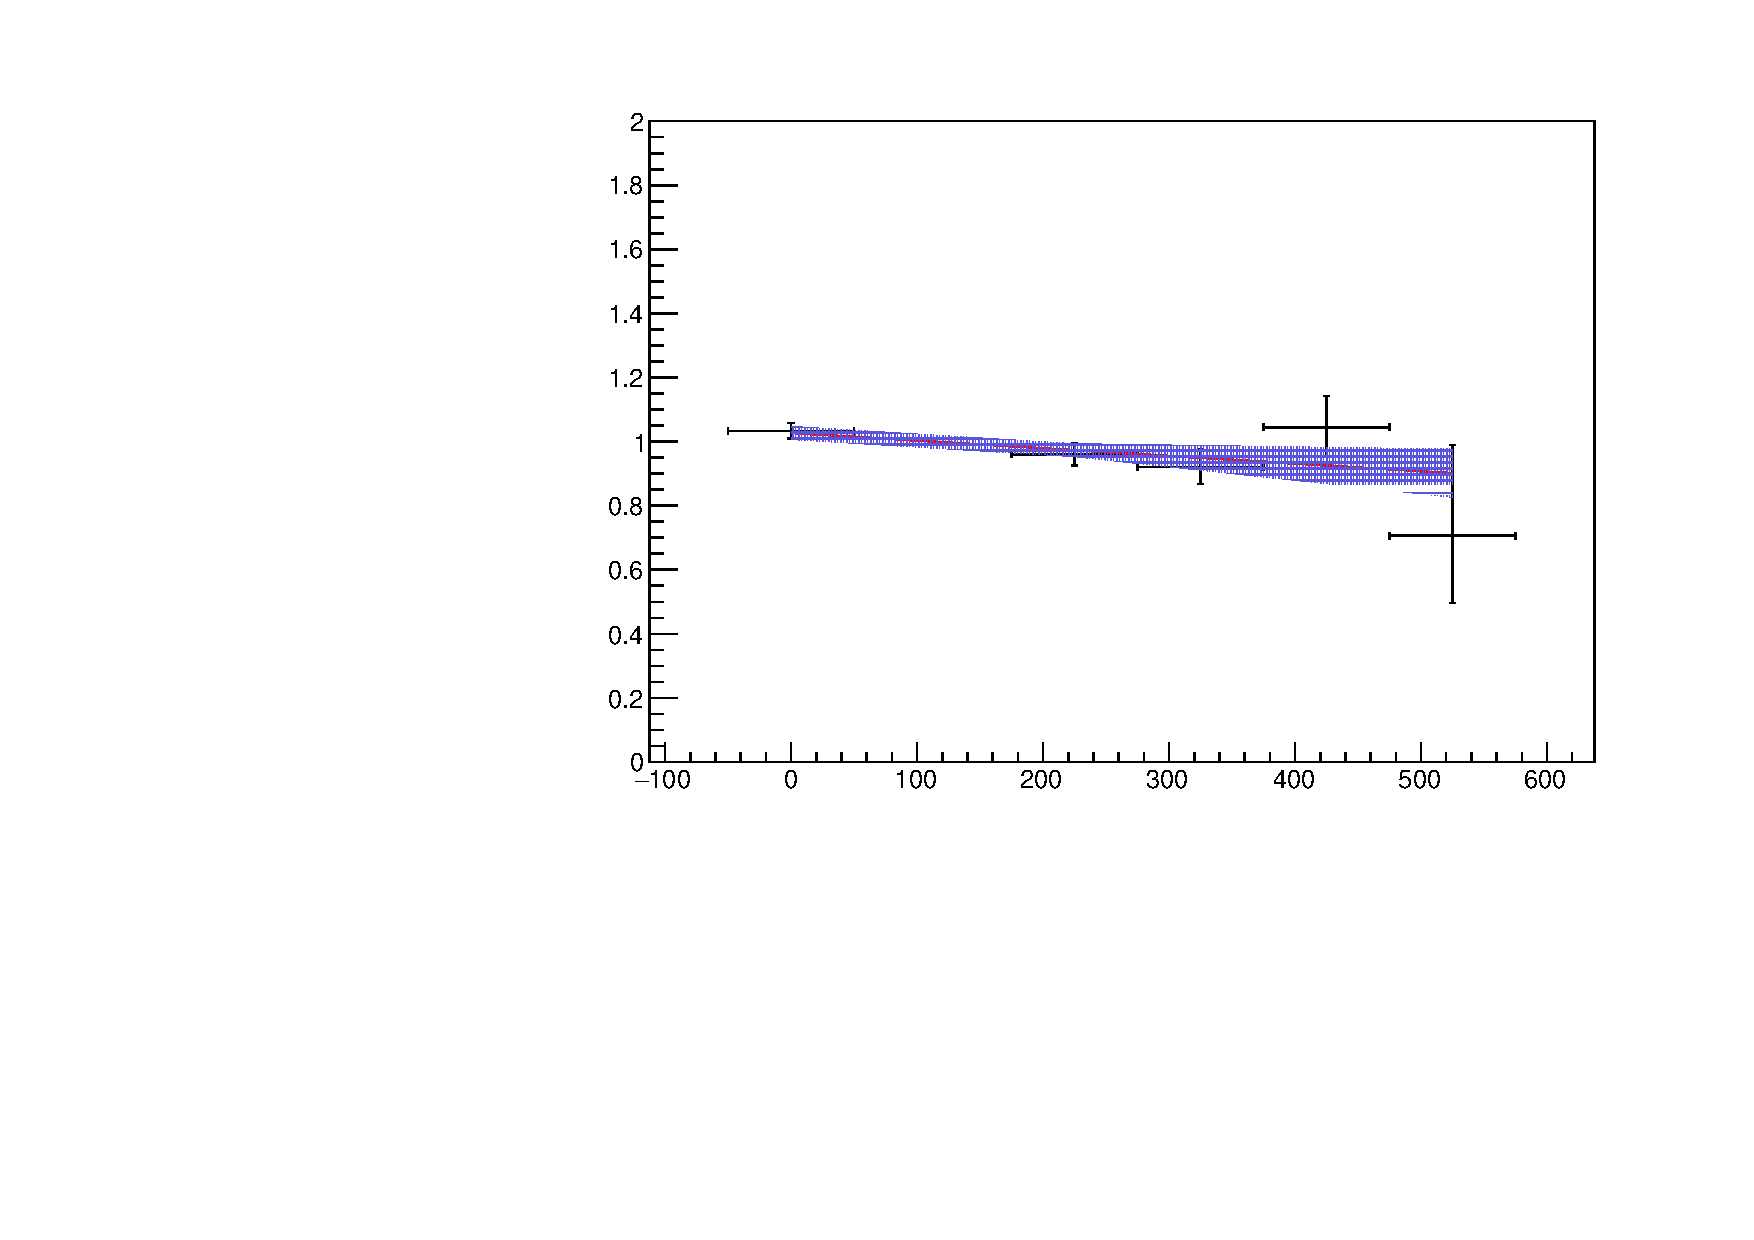
\includegraphics[width=0.5\textwidth]{figures/mhtTemplate/examples/Mu/ht500_600_control_eq0b_eq4j_Mu.pdf}
  }\\
  \subfigure[\mmj,2b, 2a category and \scalht 300-350\GeV bin]{
    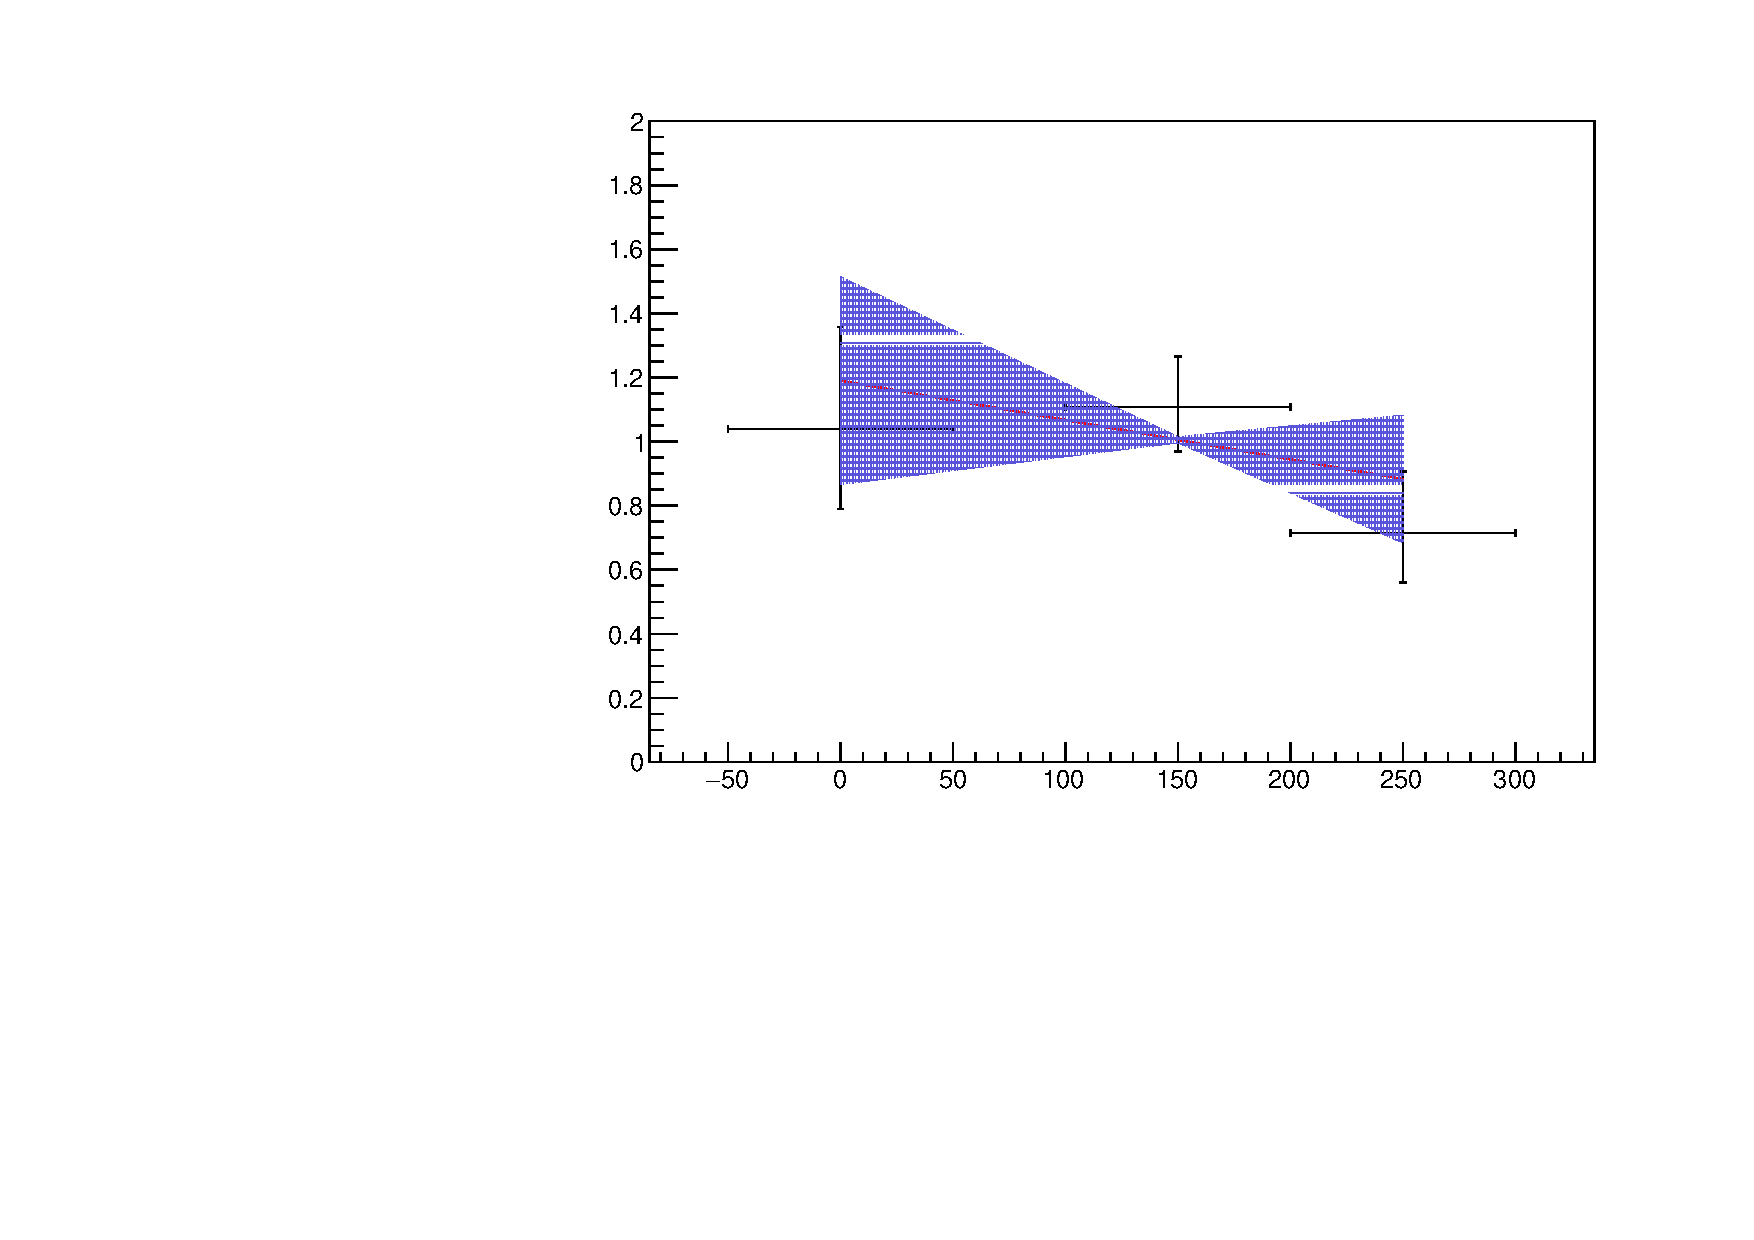
\includegraphics[width=0.5\textwidth]{figures/mhtTemplate/examples/MuMu/ht300_350_control_eq2b_ge2a_MuMu.pdf}
  }~~
  \subfigure[\gj, 1b, 5j category and \scalht 900-1050\GeV bin]{
    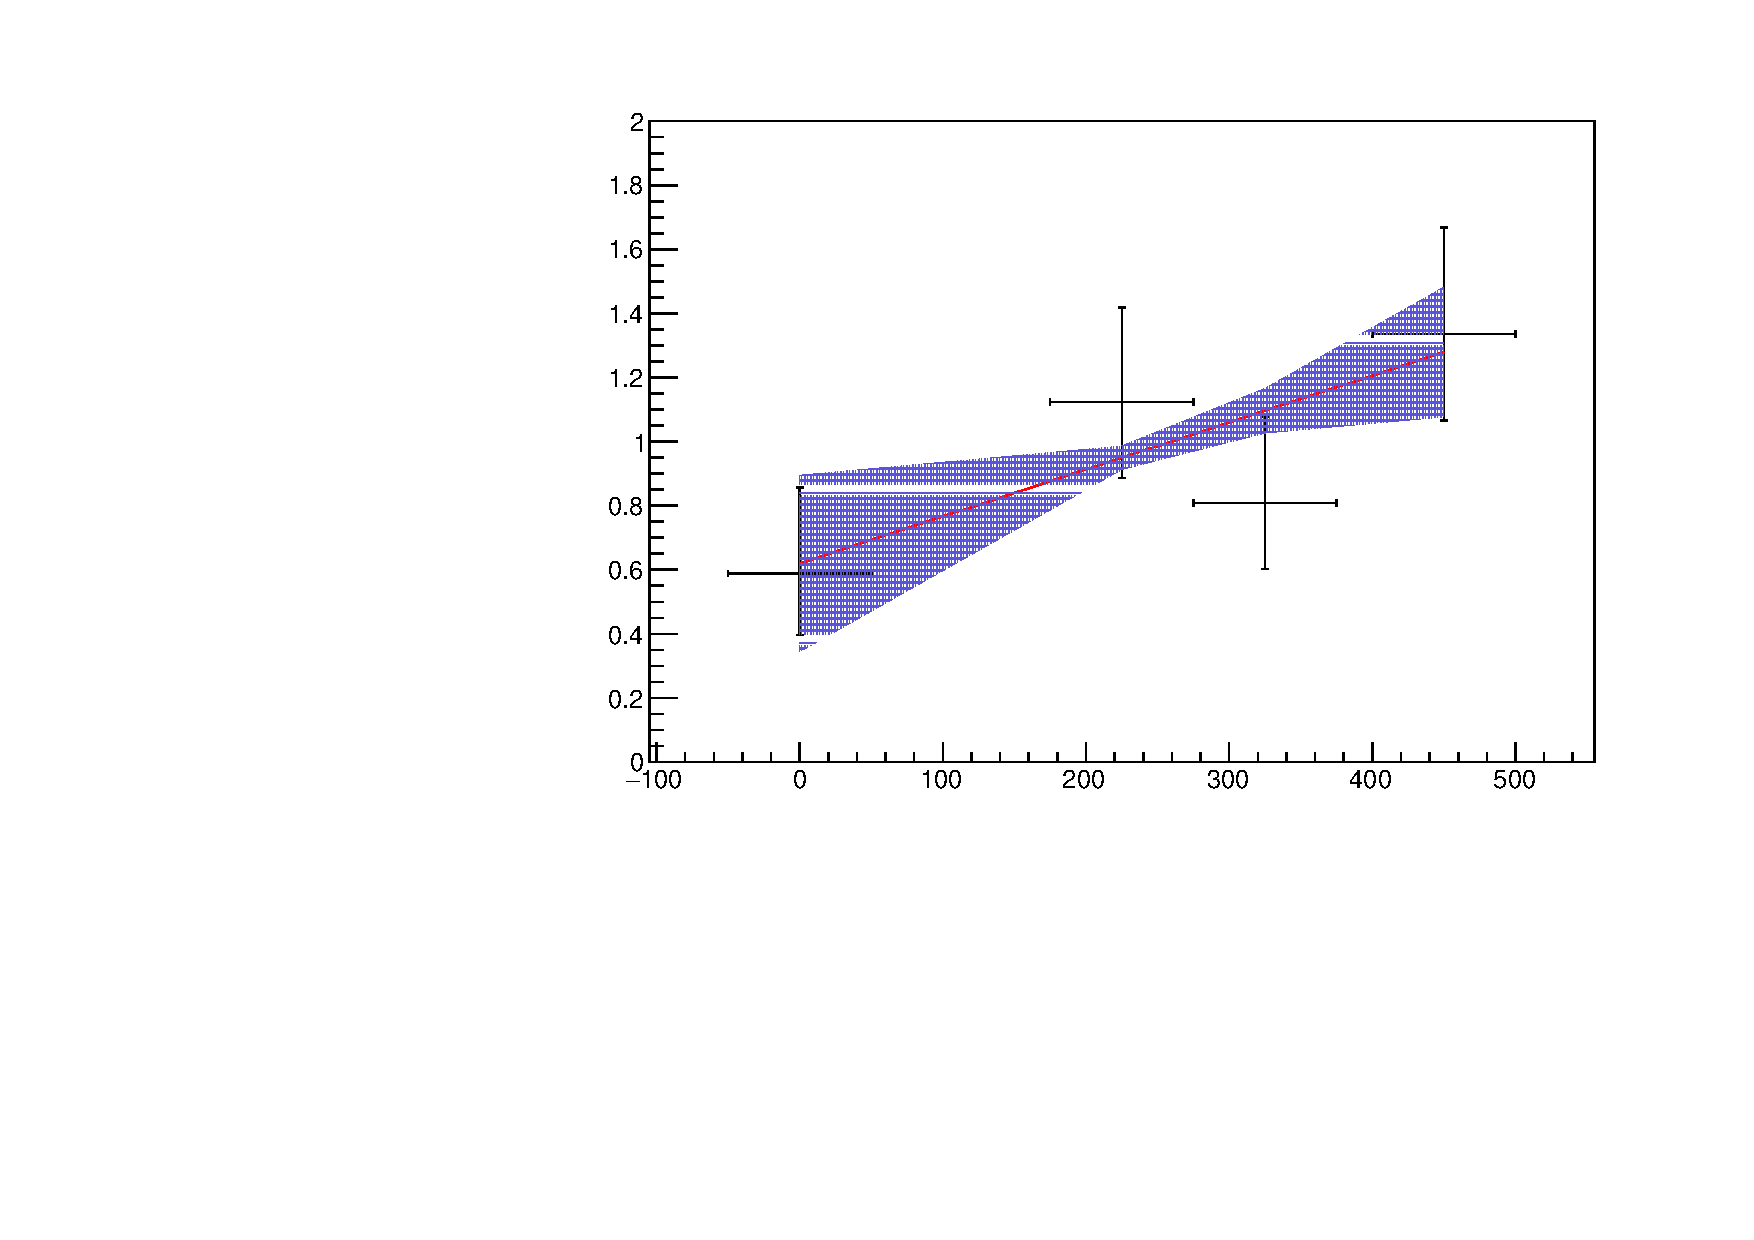
\includegraphics[width=0.5\textwidth]{figures/mhtTemplate/examples/Pho/ht900_1050_control_eq1b_eq5j_Pho.pdf}
  }\\
  \subfigure[\mj, 2b, 5j category and \scalht 600-750\GeV bin]{
    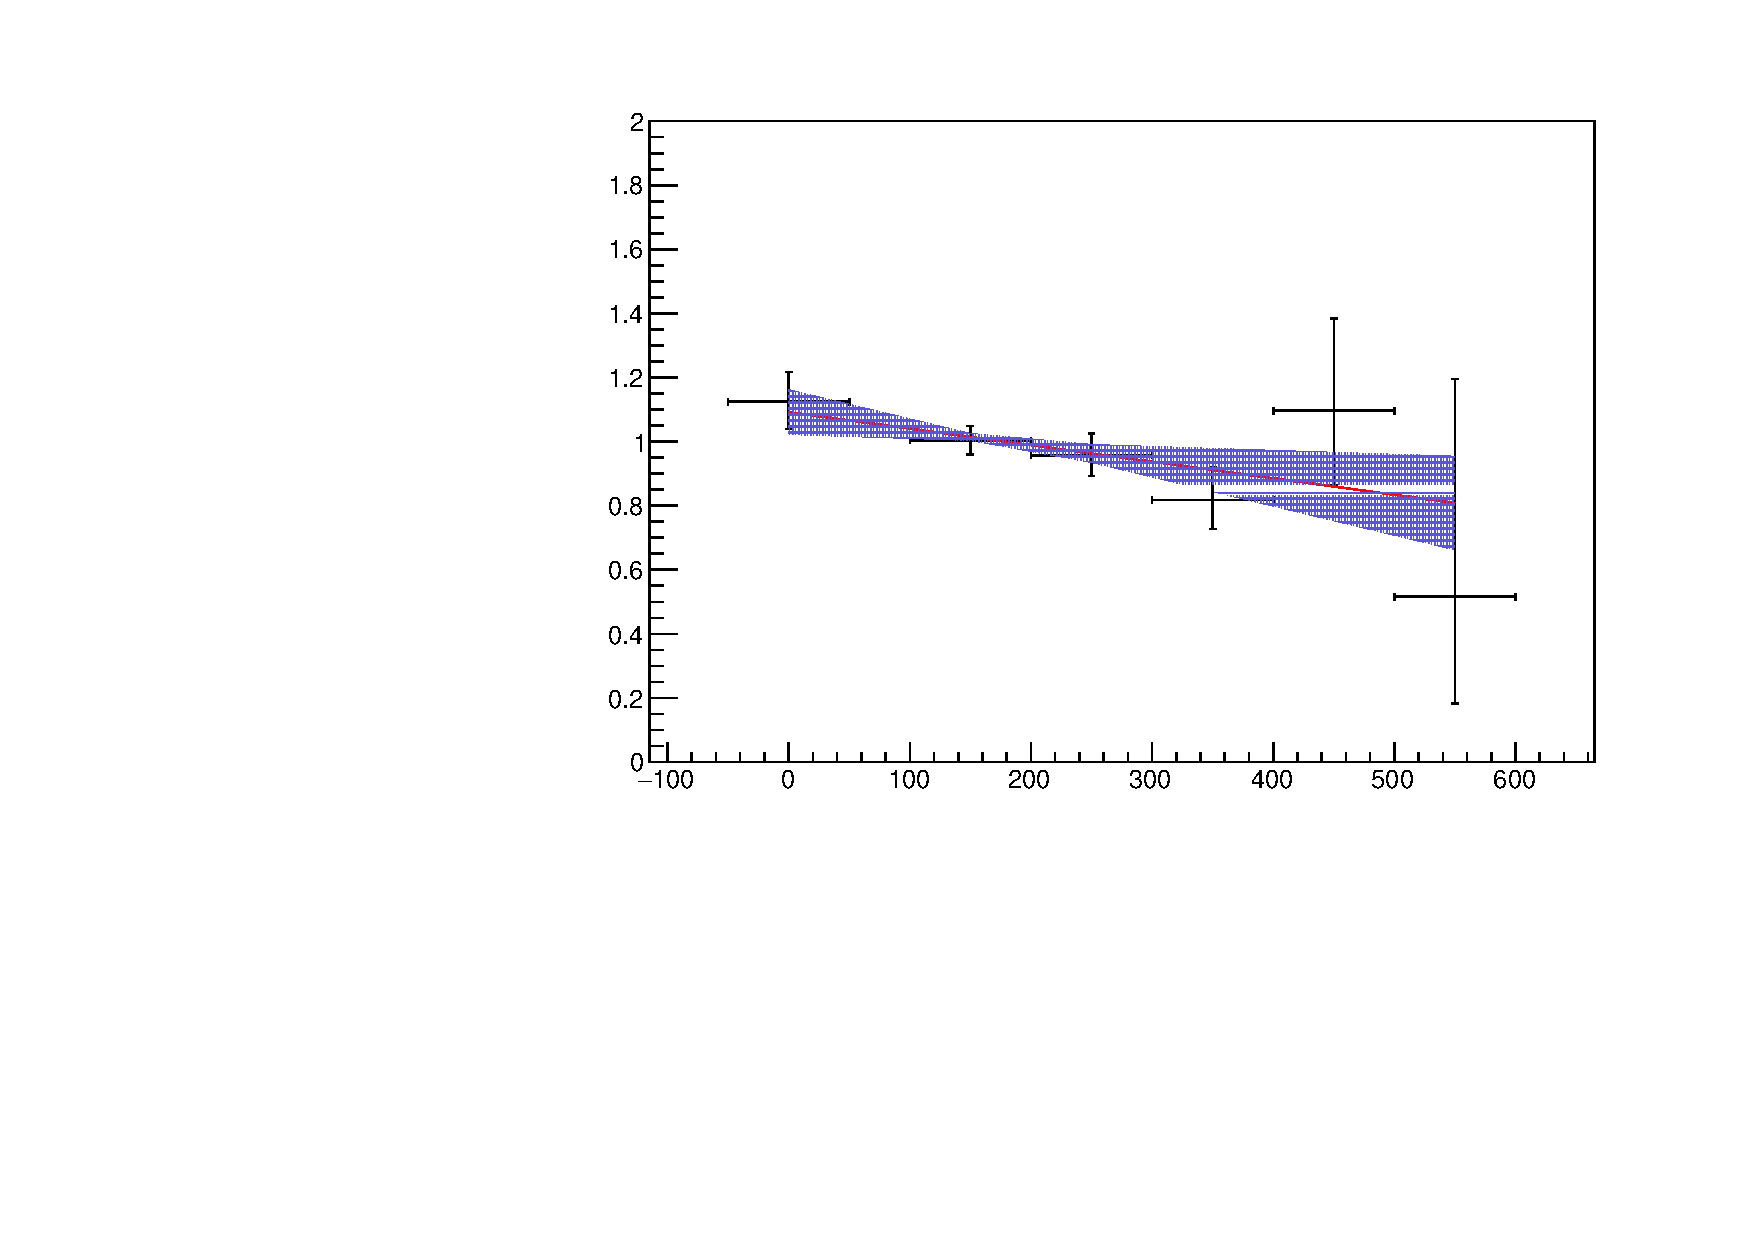
\includegraphics[width=0.5\textwidth]{figures/mhtTemplate/examples/Mu/ht600_750_control_eq2b_eq5j_Mu.pdf}
  }~~
  \subfigure[\mmj, 1b, 2j category and \scalht 400-500\GeV bin]{
    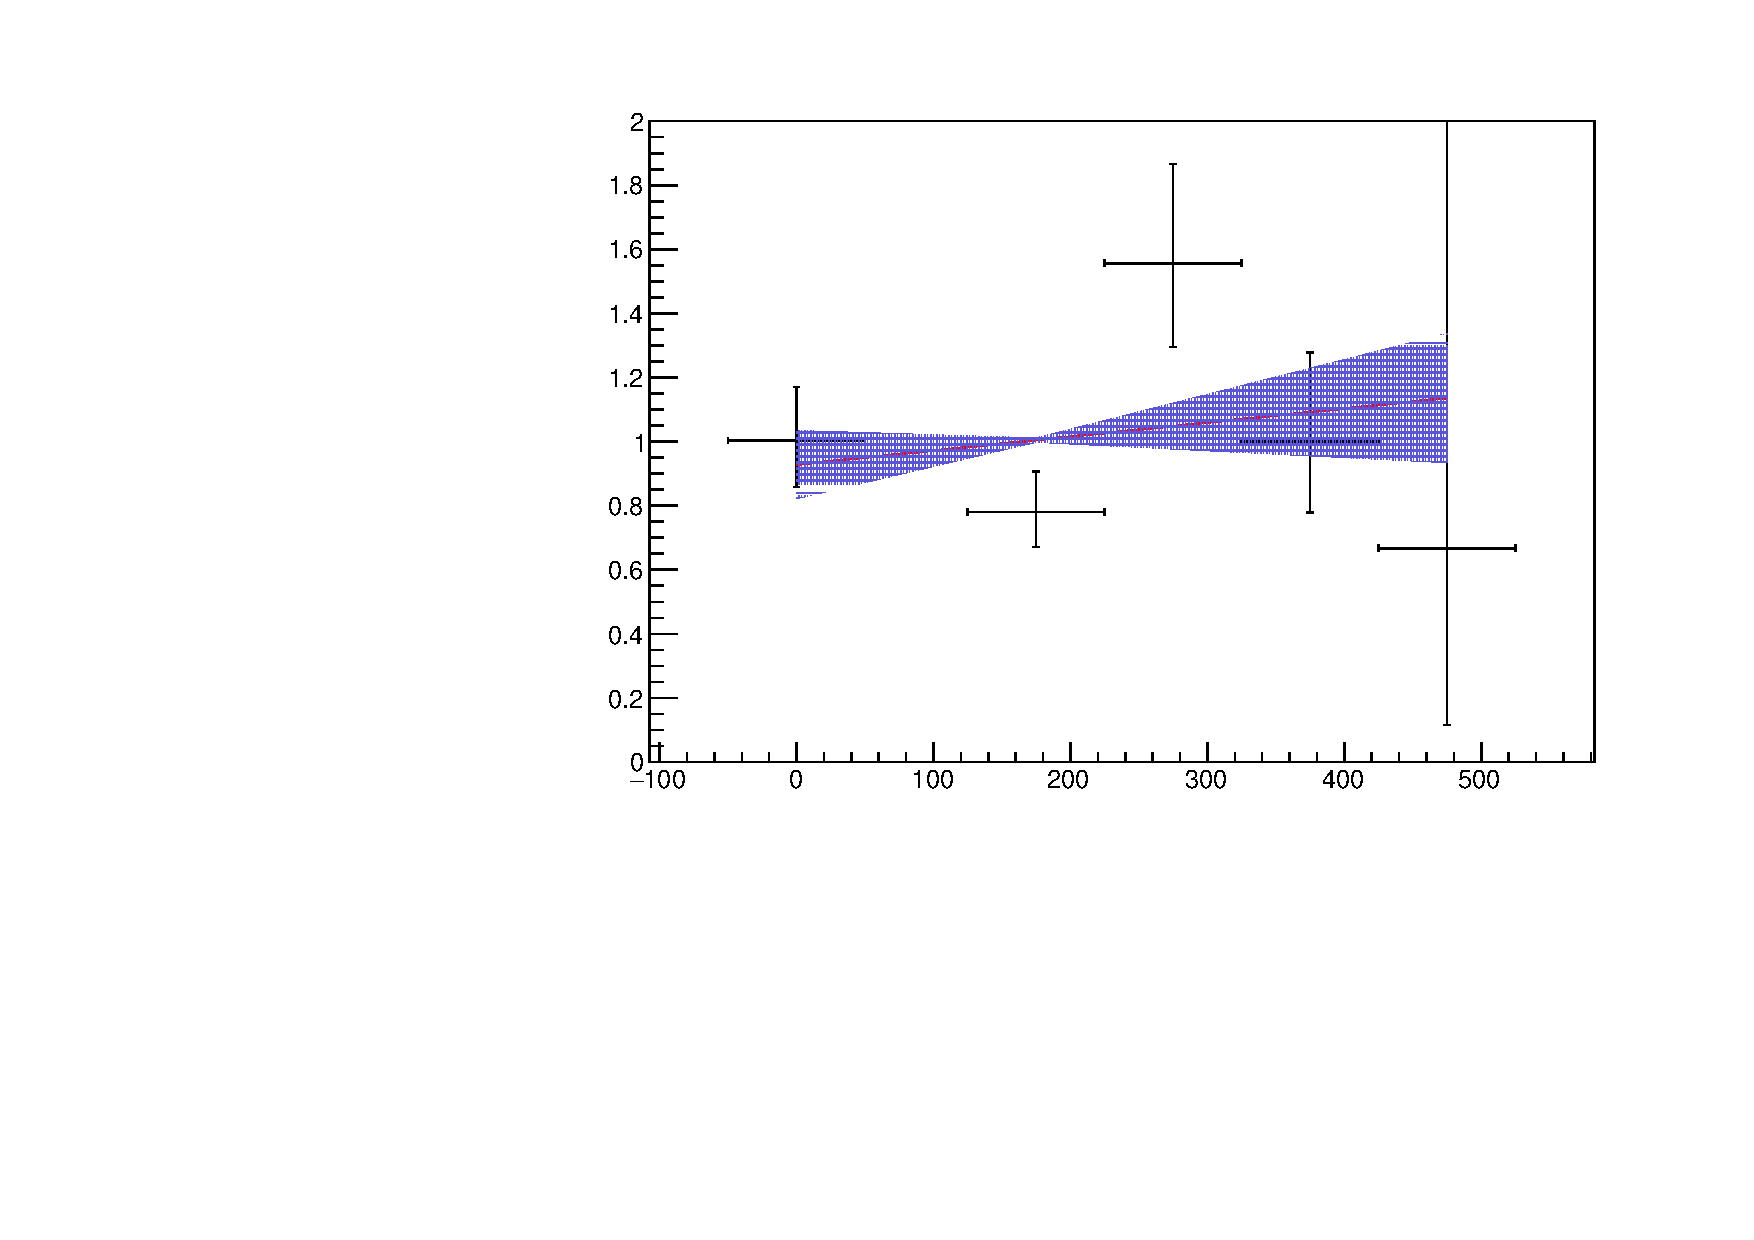
\includegraphics[width=0.5\textwidth]{figures/mhtTemplate/examples/MuMu/ht400_500_control_eq1b_eq2j_MuMu.pdf}
  }\\
  \caption{\label{fig:linearFitExamples} 
  The data/MC distribution against \mht for example categories and control regions.
  The large bias in the linear component seen in Fig.~\ref{fig:linearMotiv} is mitigated.}
\end{figure}

\begin{figure}[h!]
  \centering
  \subfigure[\mj]{
    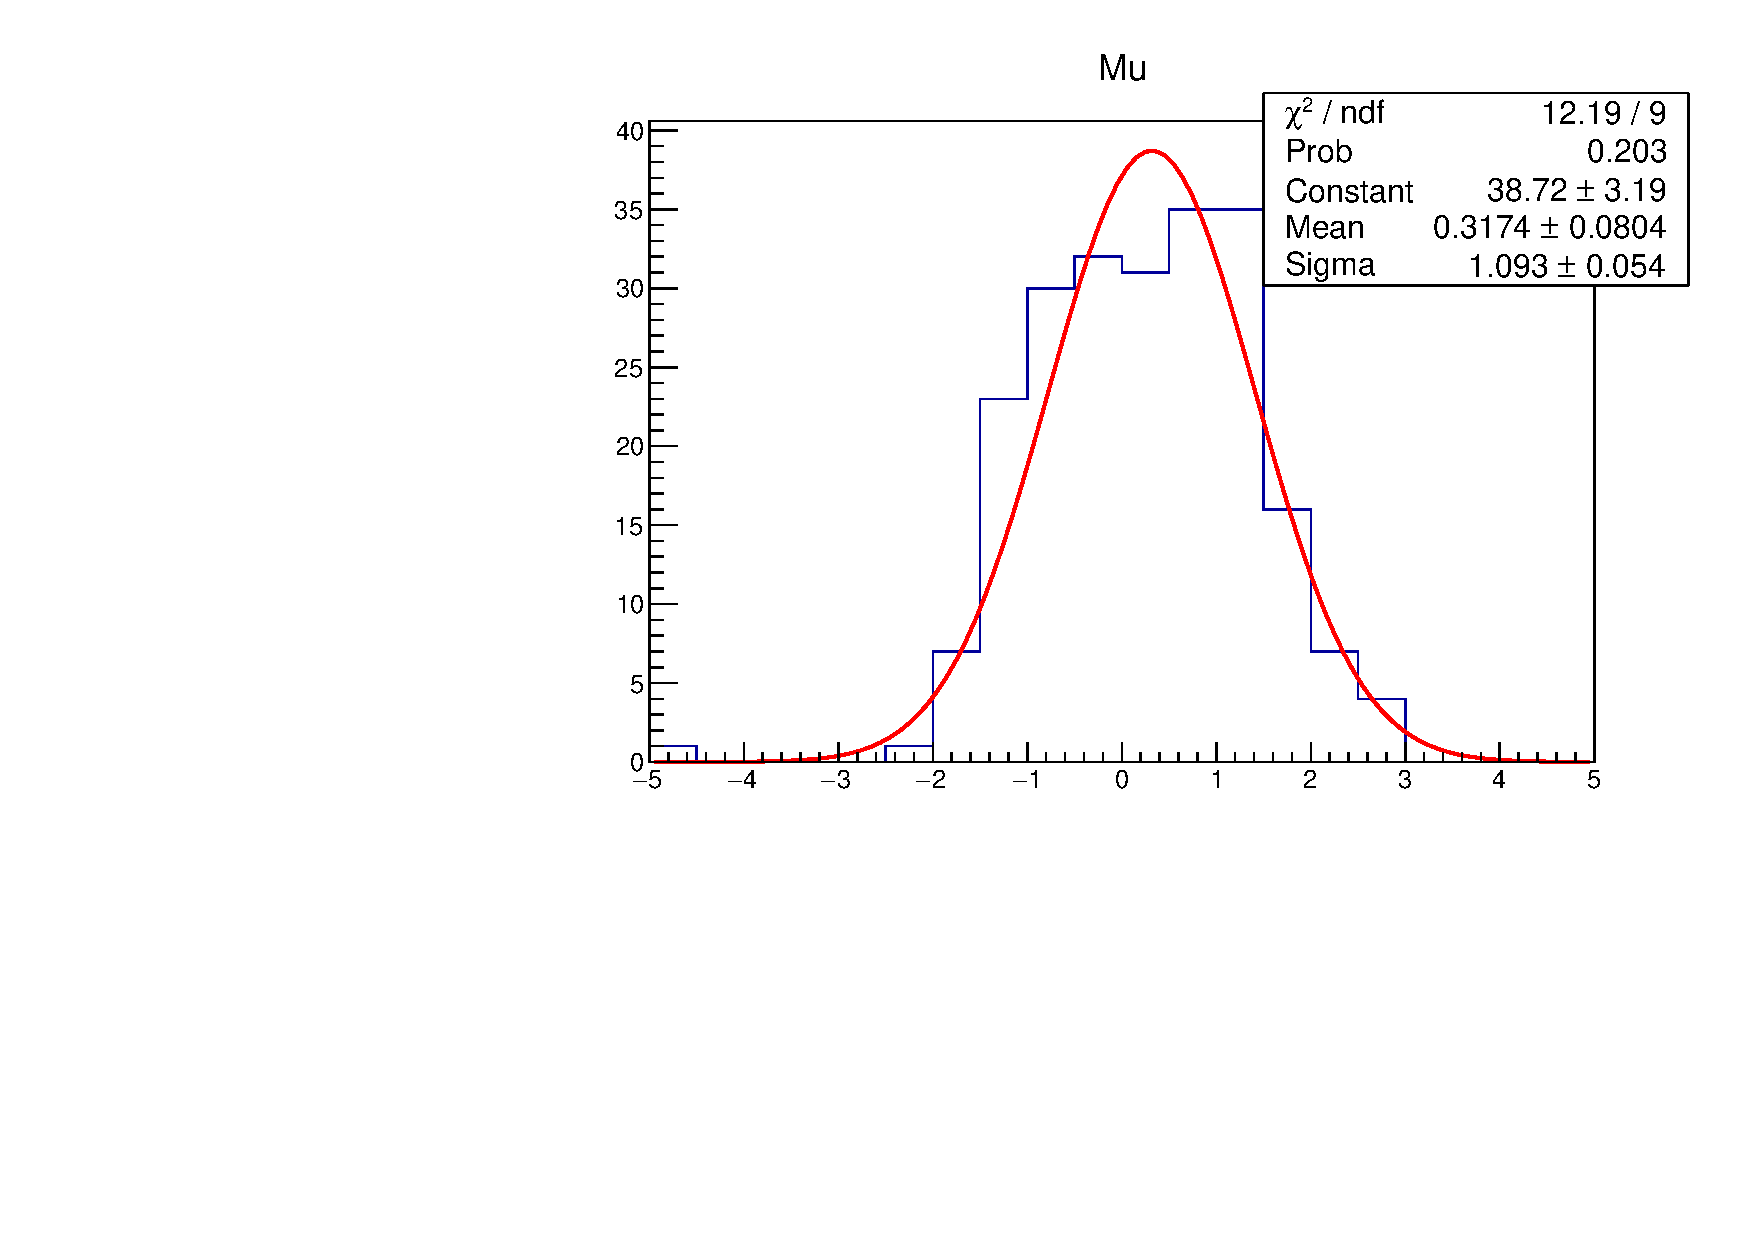
\includegraphics[width=0.5\textwidth]{figures/mhtTemplate/pulls/Mu}
  }~~
  \subfigure[\gj]{
    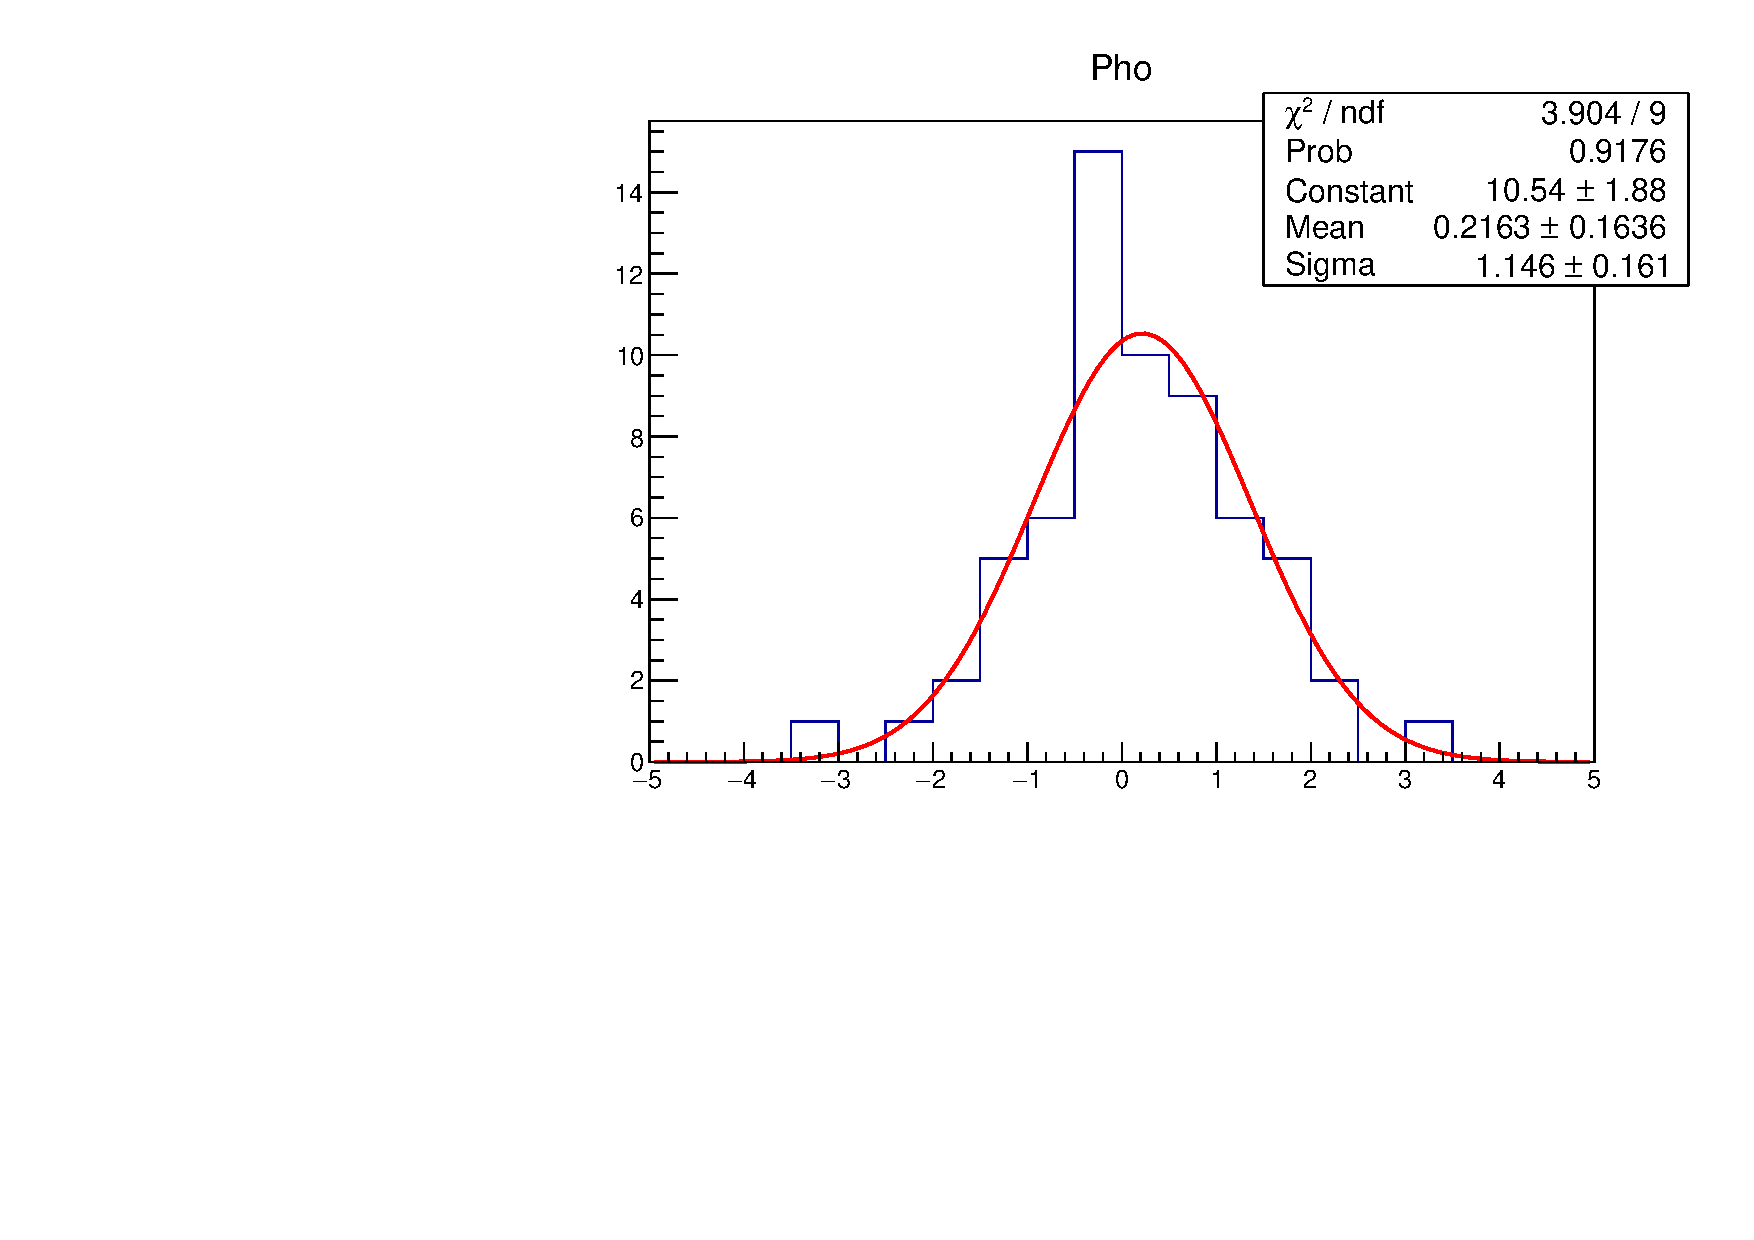
\includegraphics[width=0.5\textwidth]{figures/mhtTemplate/pulls/Pho}
  }\\
  \subfigure[\mmj]{
    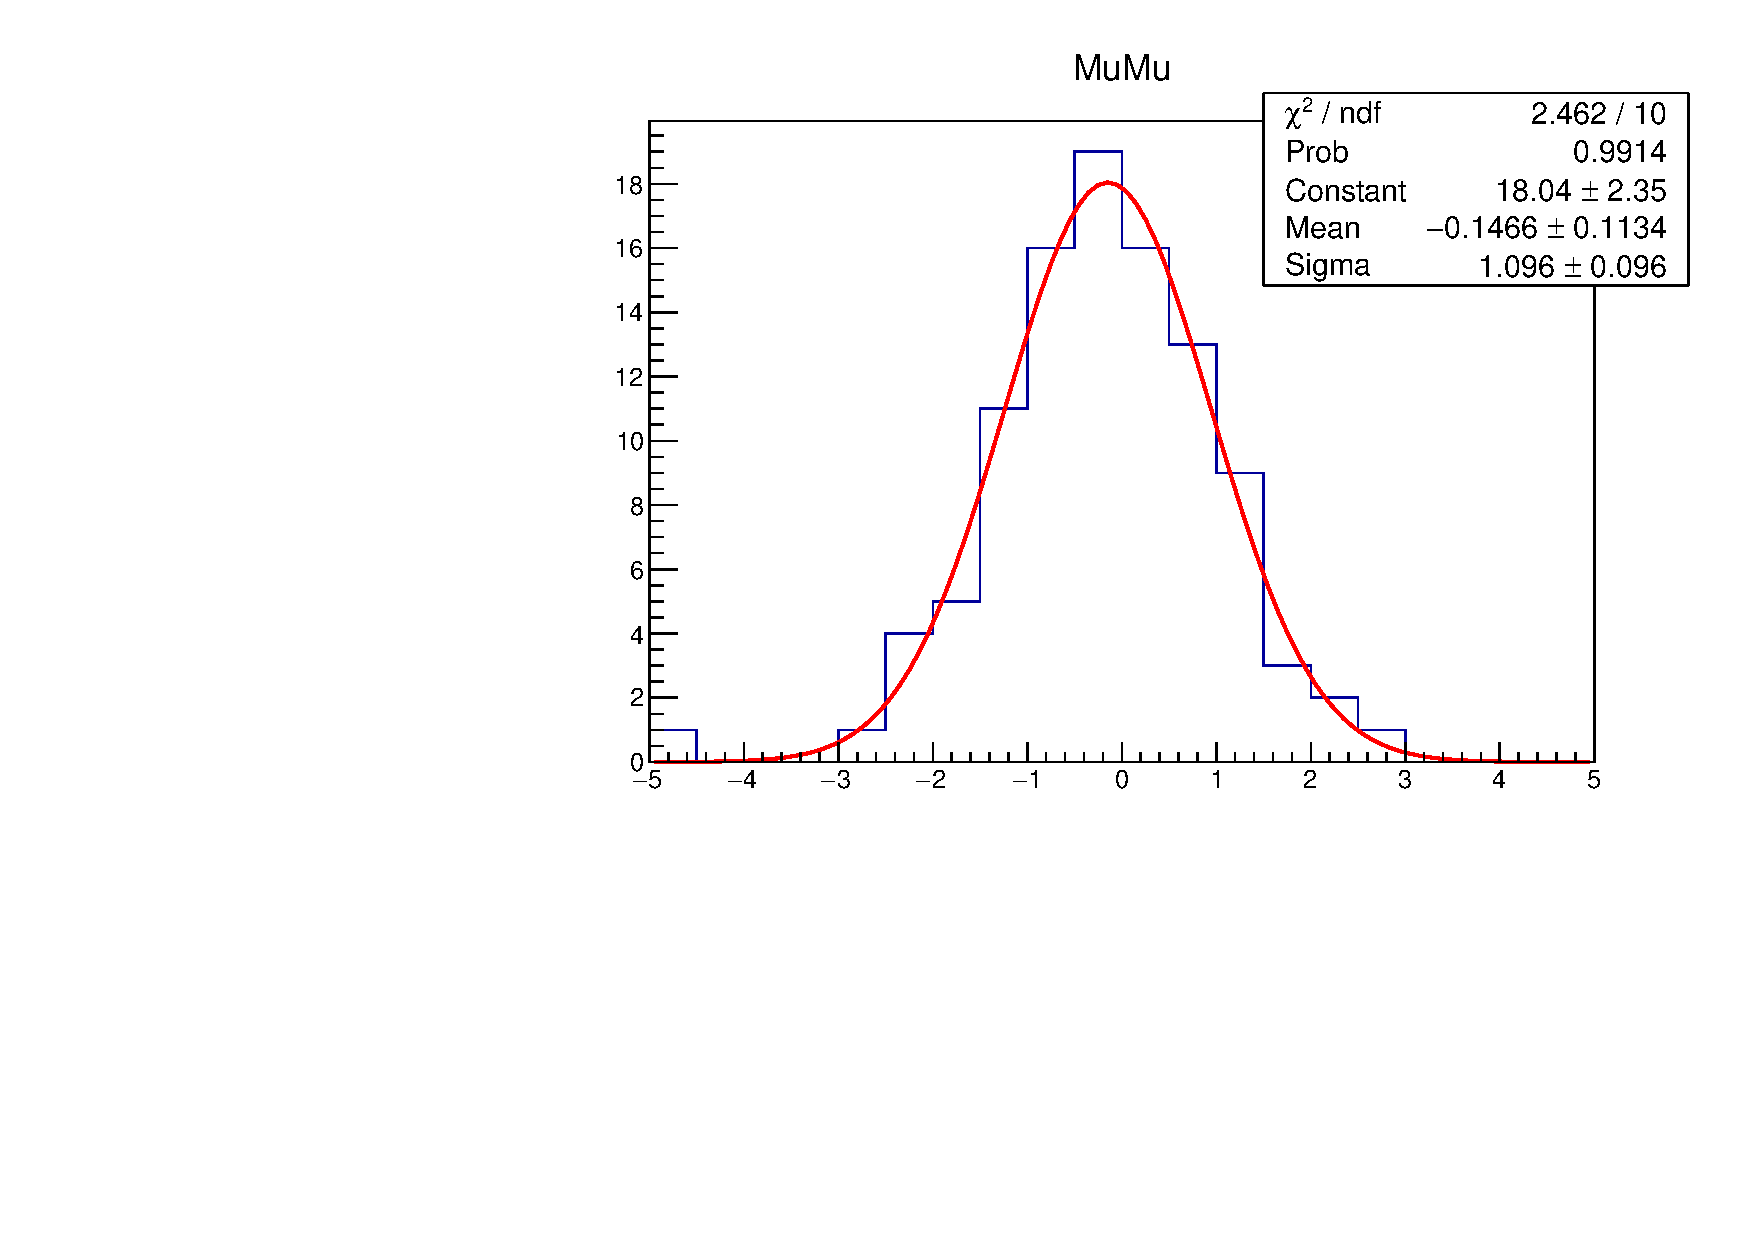
\includegraphics[width=0.5\textwidth]{figures/mhtTemplate/pulls/MuMu}
  }~~
  \\
  \caption{\label{fig:pulls} 
  The pull distribution of the linear parameter from the flat hypothesis showing no large significant bias.}
\end{figure}
\begin{figure}[h!]
  \centering
  \subfigure[\mj]{
    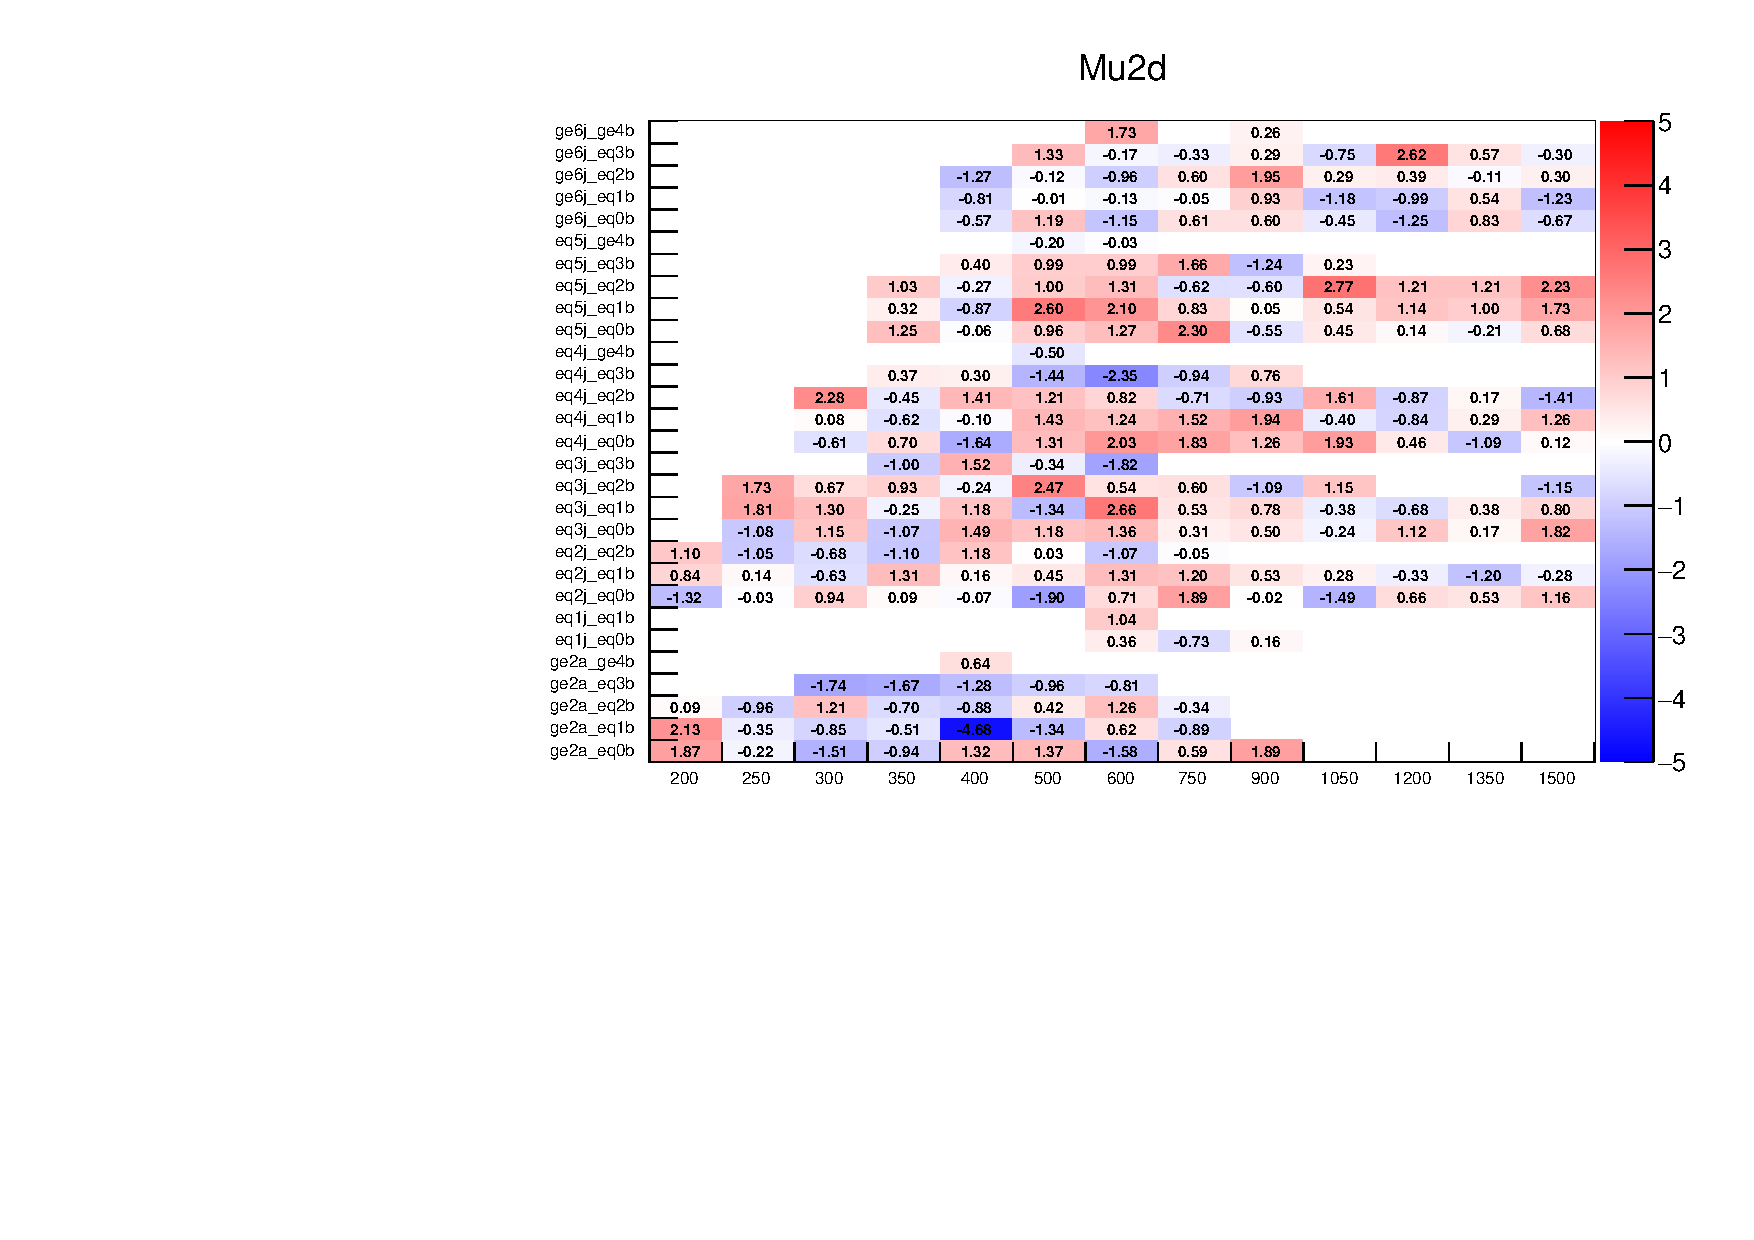
\includegraphics[width=0.5\textwidth]{figures/mhtTemplate/pulls/Mu_2D}
  }~~
  \subfigure[\gj]{
    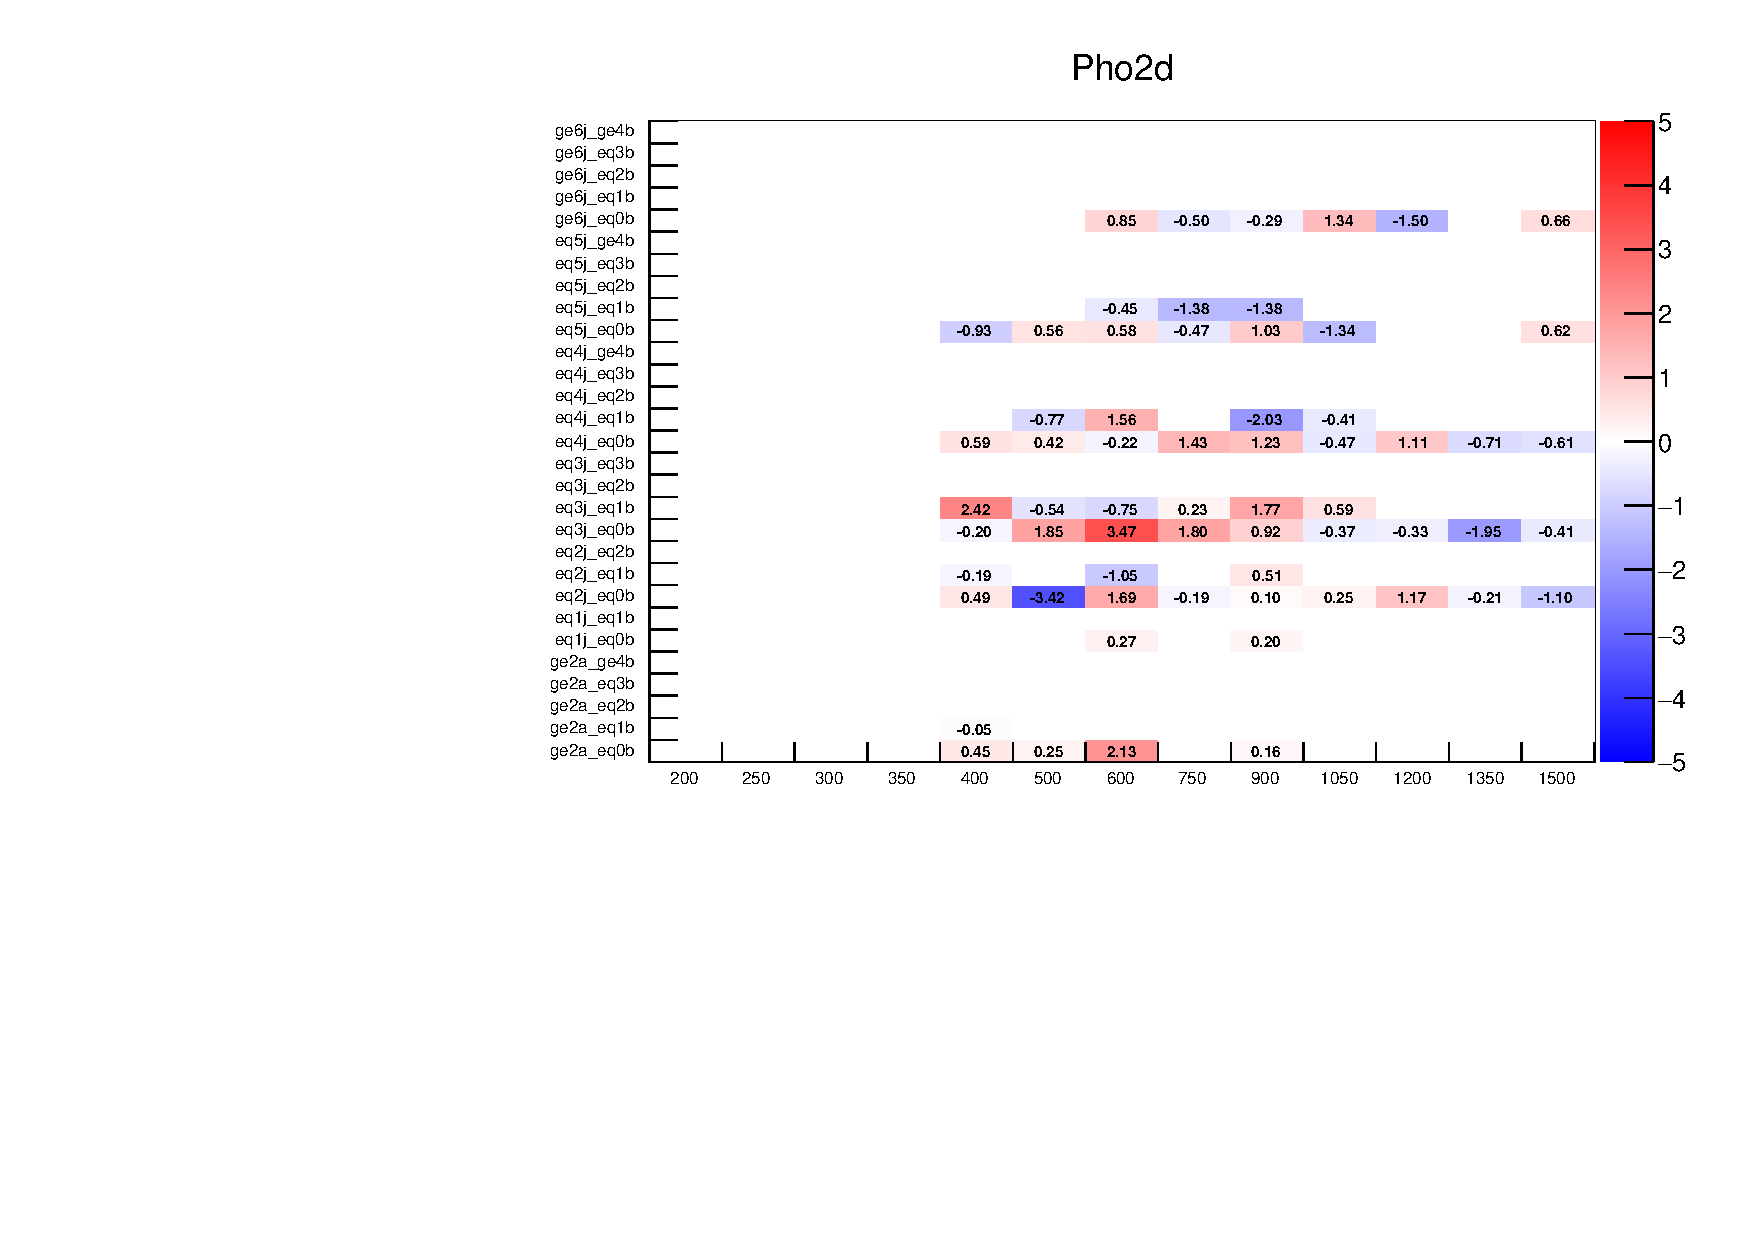
\includegraphics[width=0.5\textwidth]{figures/mhtTemplate/pulls/Pho_2D}
  }\\
  \subfigure[\mmj]{
    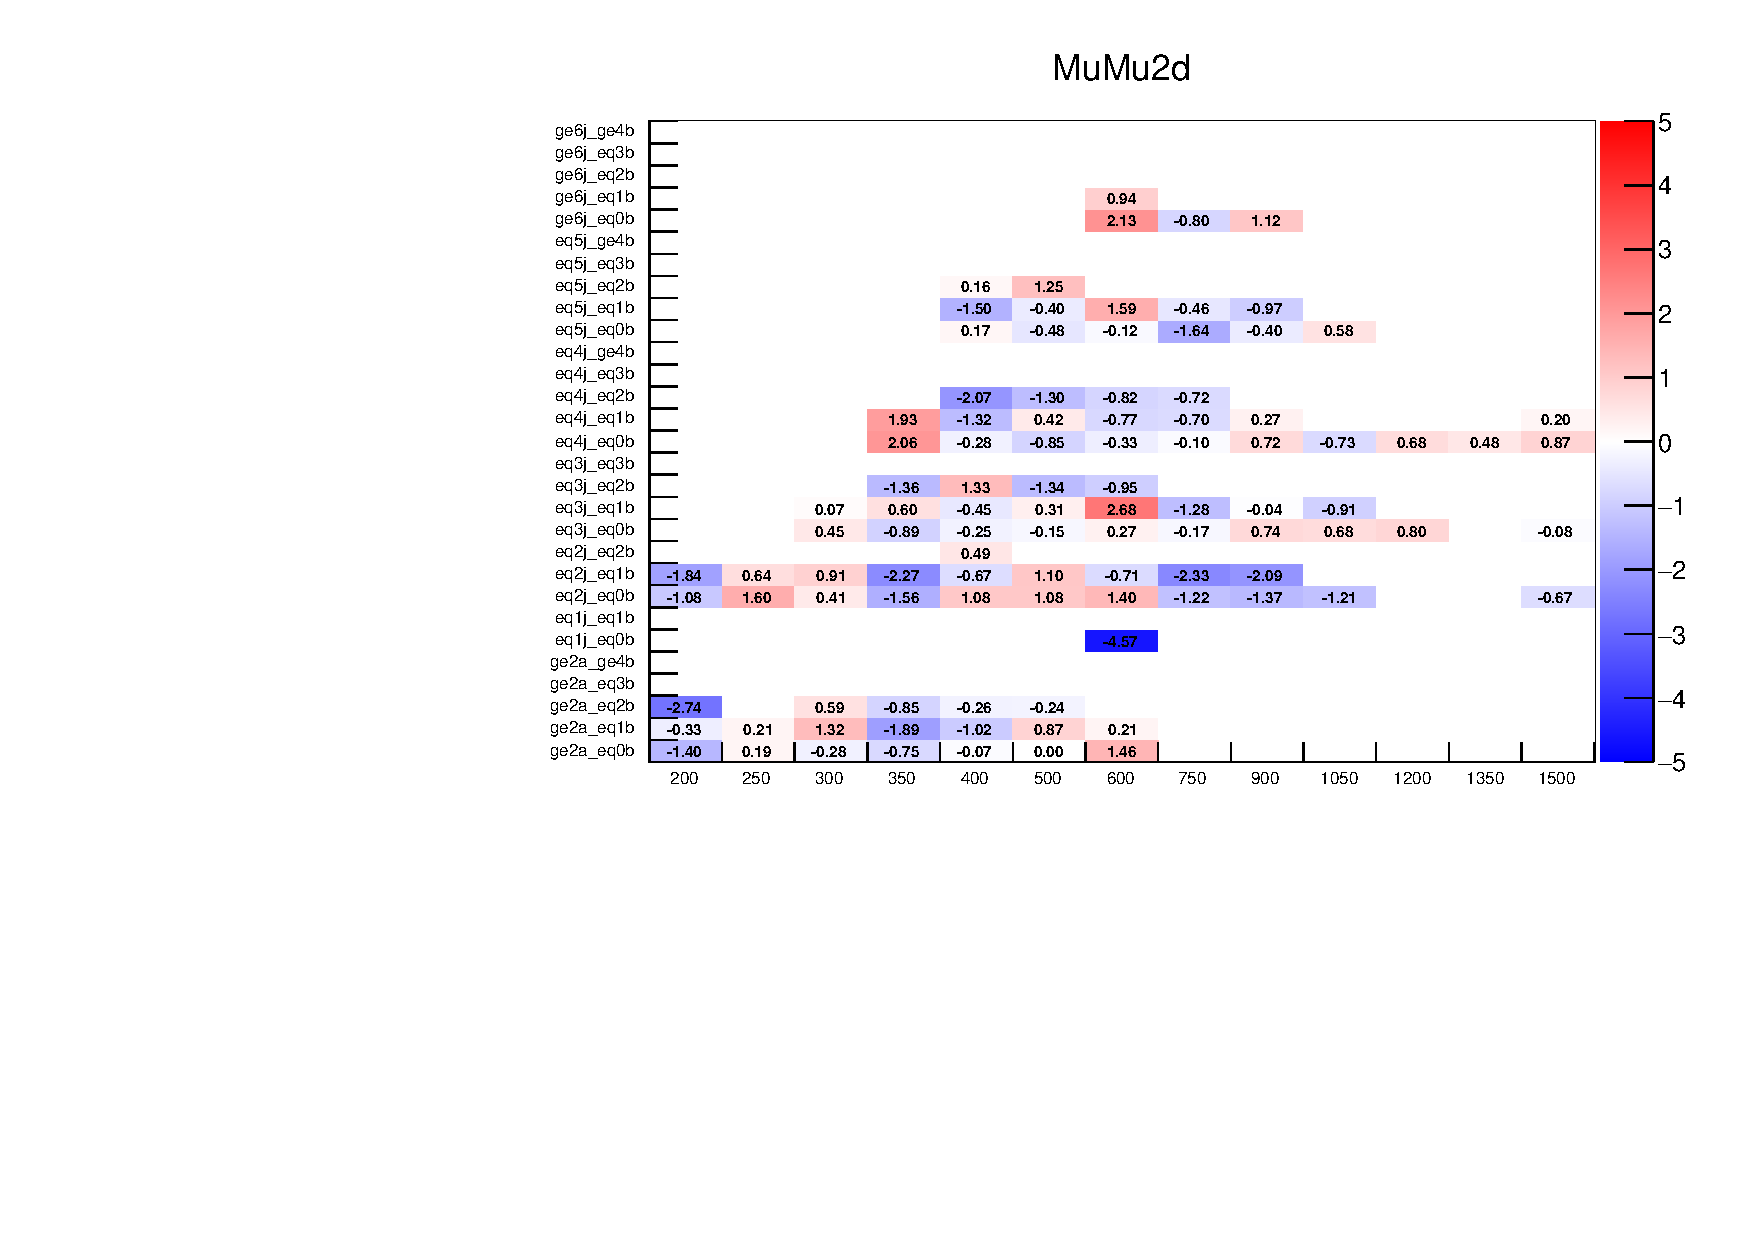
\includegraphics[width=0.5\textwidth]{figures/mhtTemplate/pulls/MuMu_2D}
  }~~
  \\
  \caption{\label{fig:frenchFlagPulls} The pull distribution of the linear parameter from the flat hypothesis across all
  \scalht bins and categories. There are no pulls for the \scalht binned are approximately consistent with gaussian scatter}
\end{figure}

% \begin{figure}[h!]
%   \centering
%   \subfigure[\mj]{
%     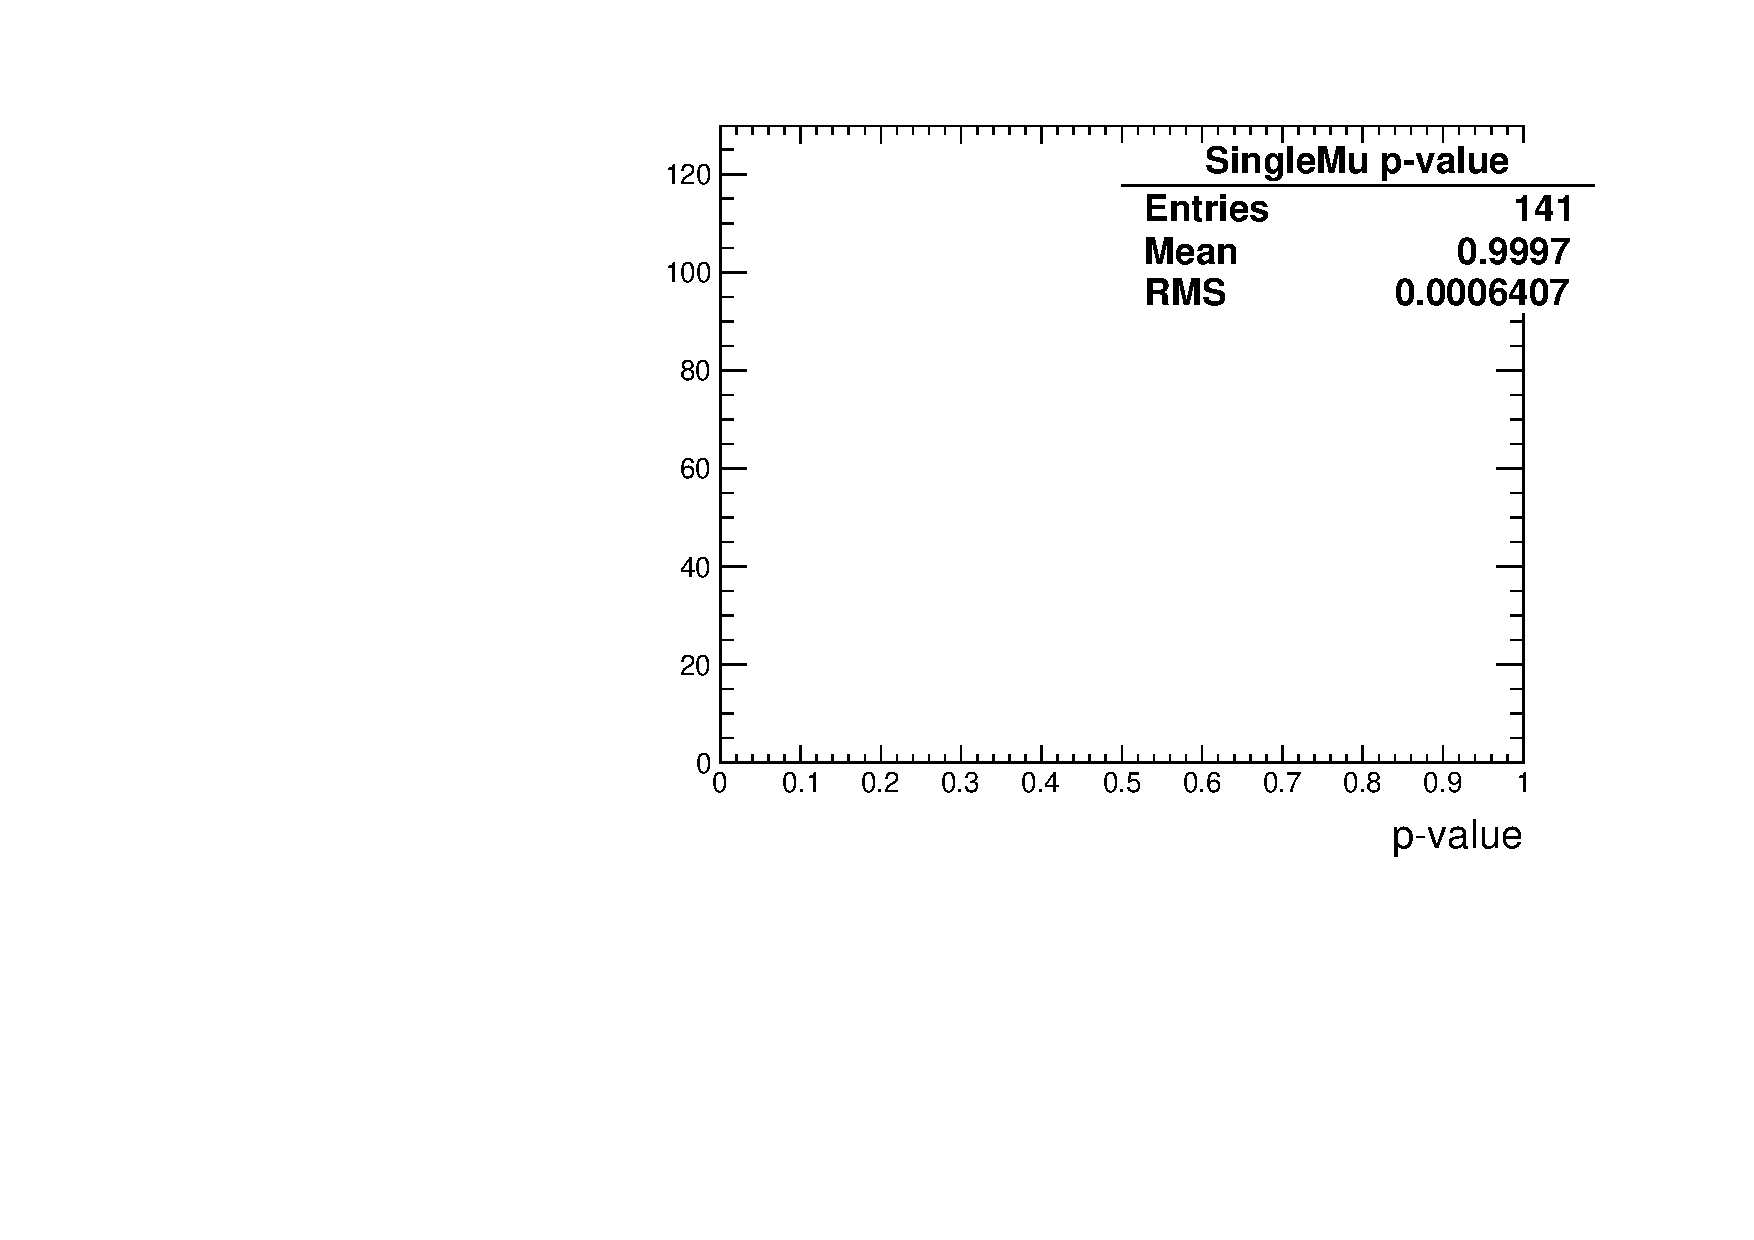
\includegraphics[width=0.5\textwidth]{figures/template2016Data/shapeOutput12Fb/scale_ht_variable_mht/SingleMu/fitOut/Linear2DShiftMean/pValue_Linear2DShiftMean_SingleMu.pdf}
%   }~~
%   \subfigure[\gj]{
%     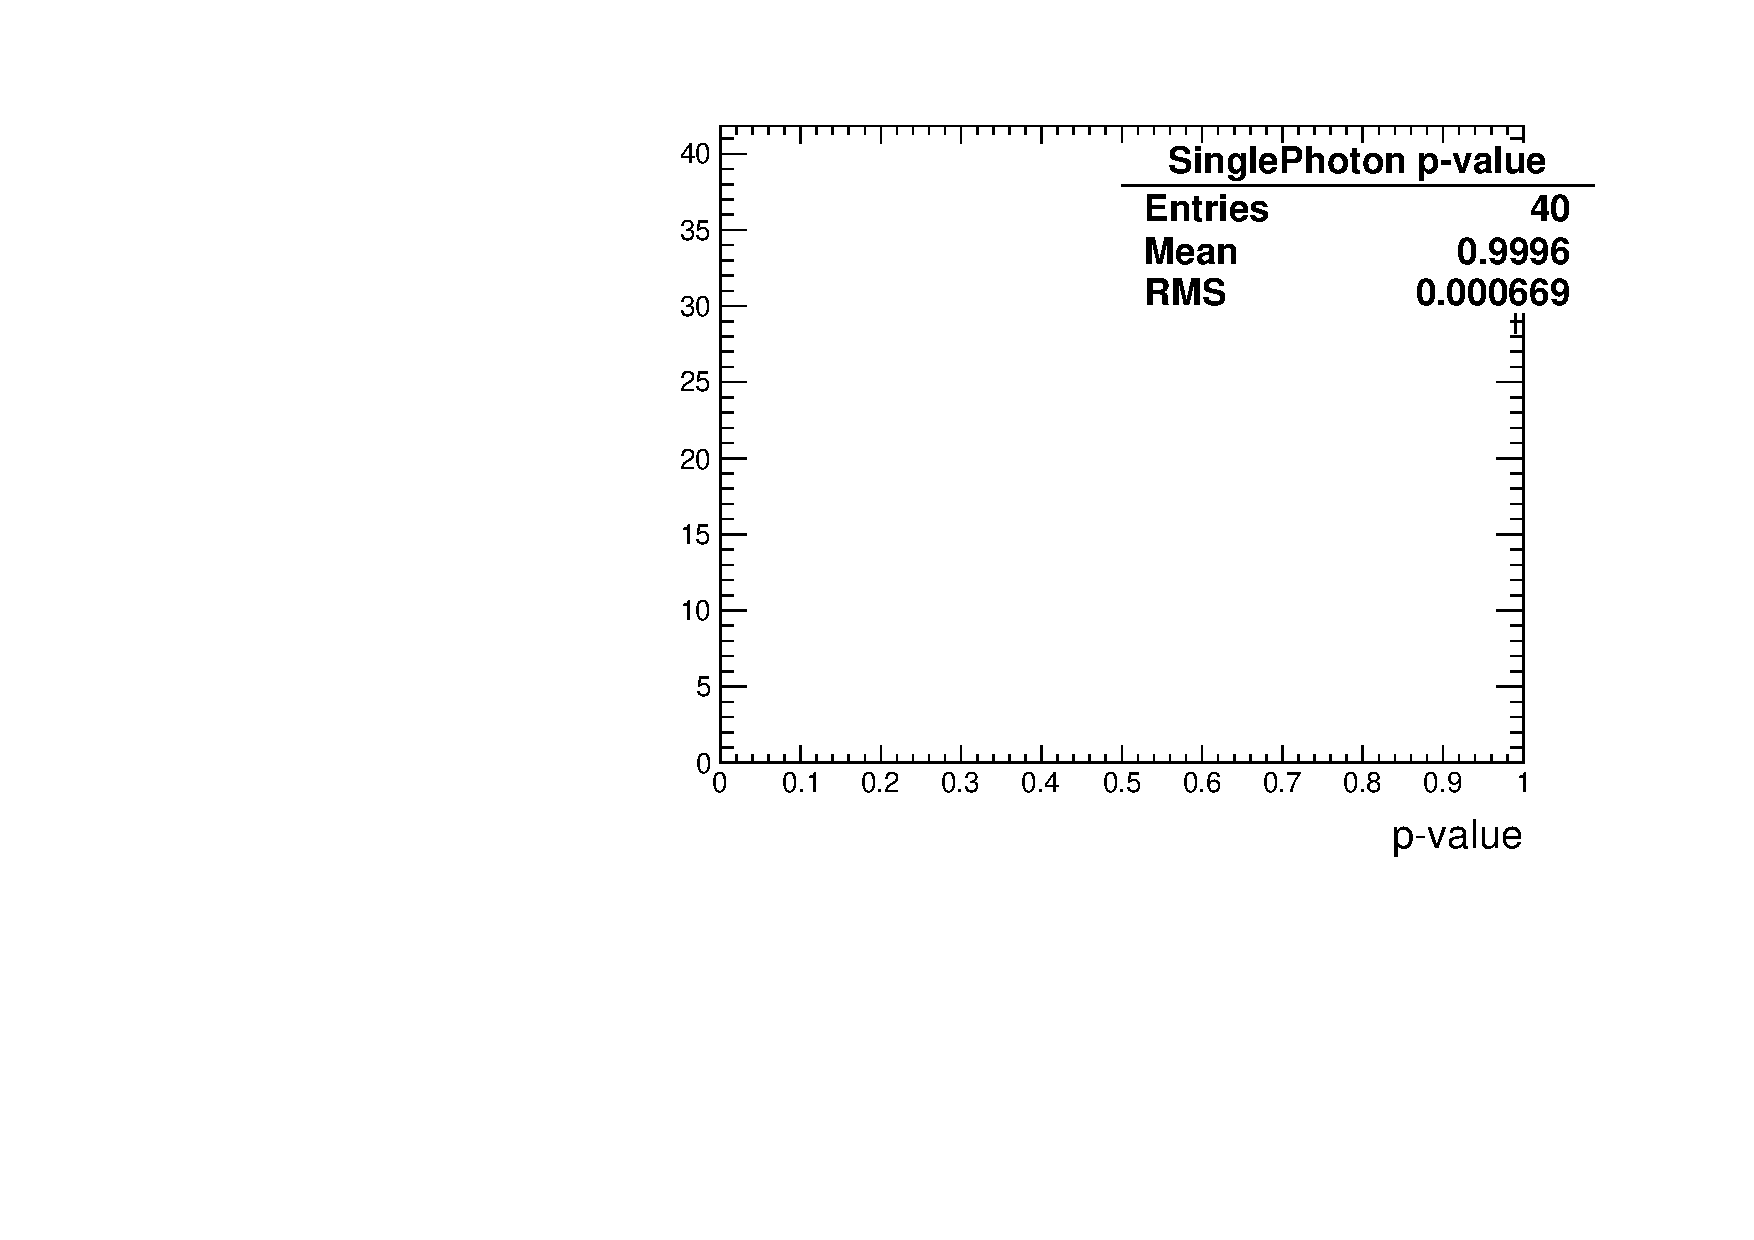
\includegraphics[width=0.5\textwidth]{figures/template2016Data/shapeOutput12Fb/scale_ht_variable_mht/SinglePhoton/fitOut/Linear2DShiftMean/pValue_Linear2DShiftMean_SinglePhoton.pdf}
%   }\\
%   \subfigure[\mmj]{
%     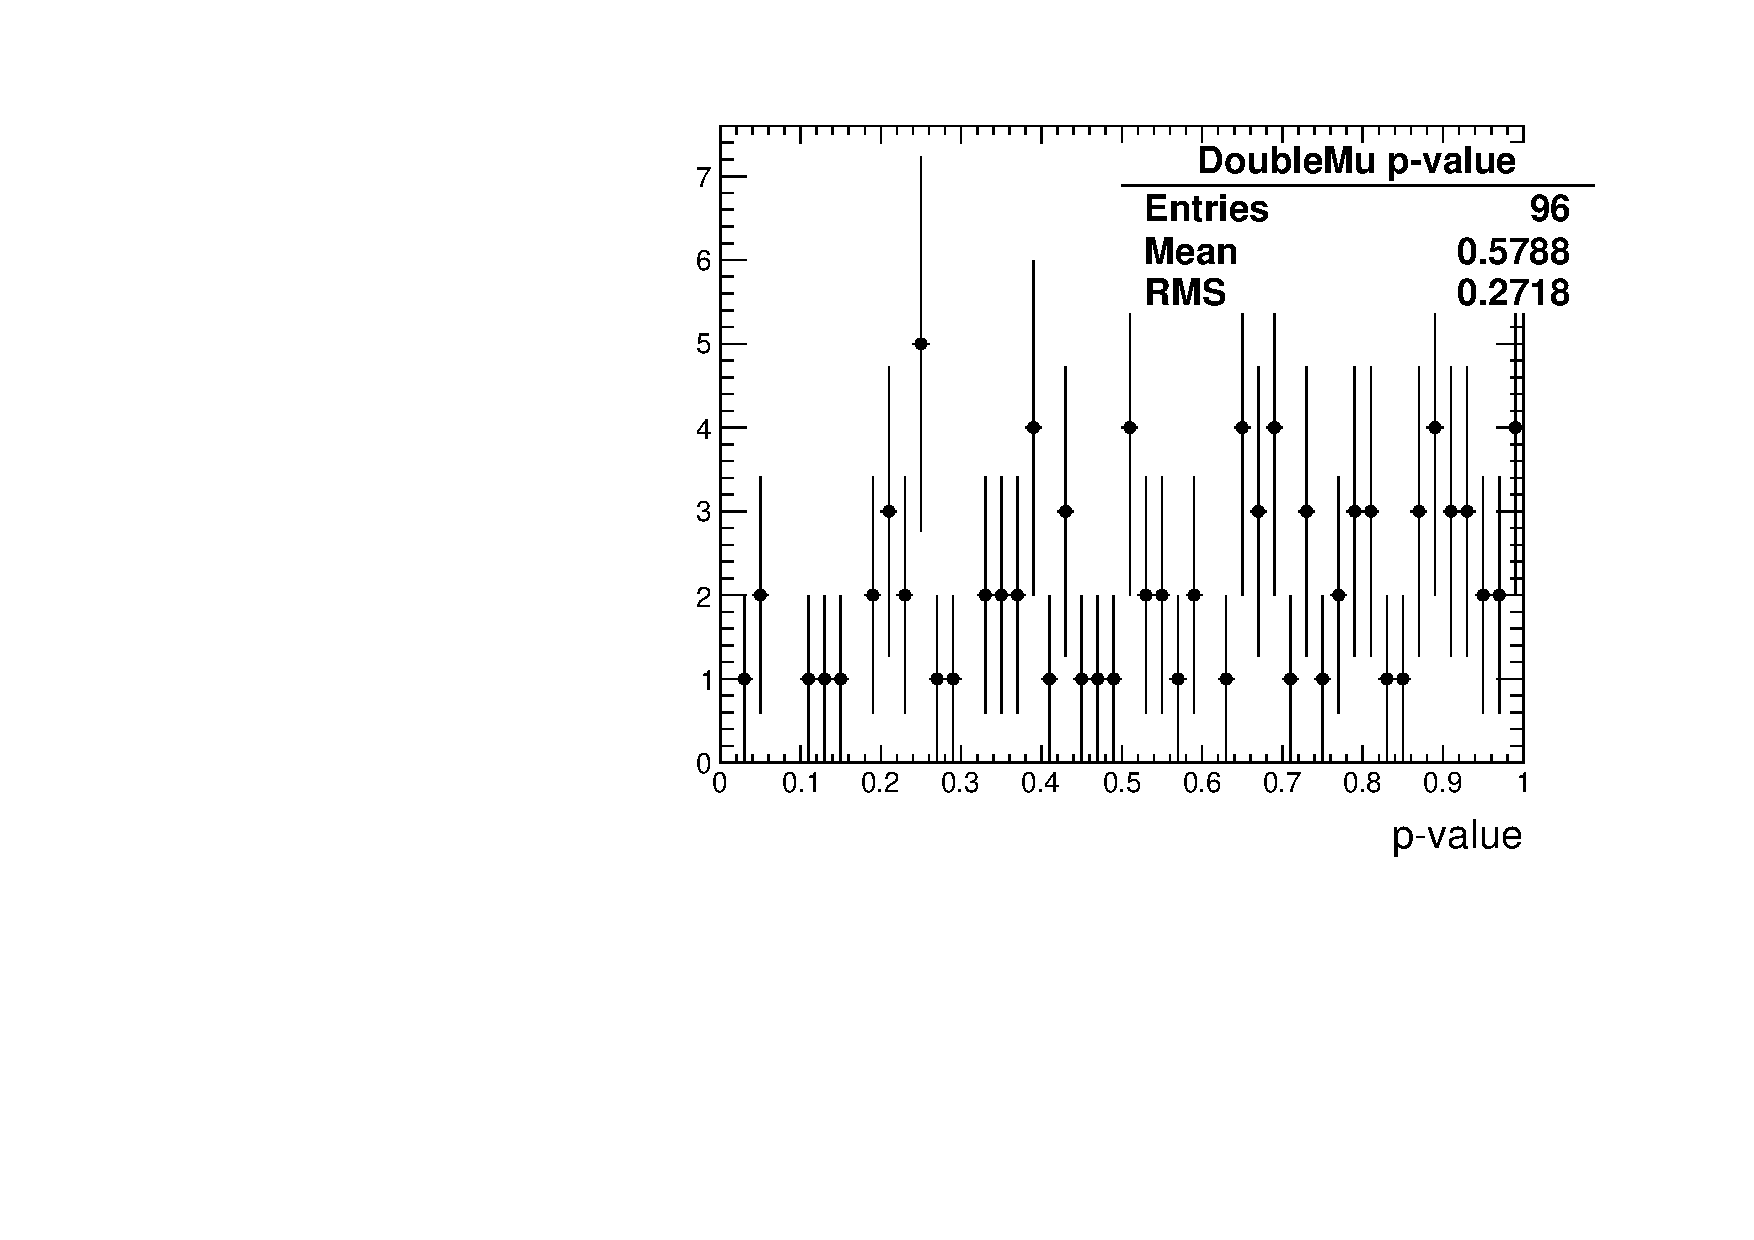
\includegraphics[width=0.5\textwidth]{figures/template2016Data/shapeOutput12Fb/scale_ht_variable_mht/DoubleMu/fitOut/Linear2DShiftMean/pValue_Linear2DShiftMean_DoubleMu.pdf}
%   }~~
%   \\
%   \caption{\label{fig:pValues} The distributions of the p-value for the linear fit.} 
% \end{figure}
\subsection{Deriving systematics on the \texorpdfstring{\mht}~dimension}
\label{sec:systMhtDimension}

Systematics in the \mht dimension are extracted using the data in the control 
regions to determine the statistical precision to which the hypothesis of zero bias can
be confirmed. In this analysis the main discriminating variables
are \njet,\nb and \scalht. Two sets of systematic uncertainties on the \mht distributions,
correlated in \scalht and \njet, are derived using data from the control regions.
The set of systematics decorrelated in \scalht allows any disagreement which 
is localised at a particular scale to be covered while the set of systematics 
decorrelated in \njet covers systematic effects localised in the
number of partons or ISR jets. The \nb dimension is not decorrelated as this discriminating
variable is not directly related to the scale of the event and will be strongly correlated to \njet.
The sets of 7 and 5 systematics for decorrelation in \njet and \scalht respectively
are derived in data as described in the following.

Each background in the signal region (\ttbar/W  and \zInv~) is predicted 
using several control regions. In order to determine the uncertainty in
the \mht dimension a combined linear fit is made over all relevant control regions
In each case the normalisation term is decorrelated across all categories while the linear 
term is correlated across the correlated categories for the systematic. The 
post fit values and uncertainties of the linear parameters are shown in
Figure~\ref{fig:postFitPerNJet} and Figure~\ref{fig:postFitPerHt} for the systematics decorrelated in \njet and \scalht respectively.
The uncertainty on the linear parameters from the fit are then
used to define the up and down one sigma variations of the nominal templates in the signal region
for each systematic. As a conservative estimate, the best fit value of the parameter is 
added in quadrature to its uncertainty in order to derive the overall variation for each template.
The templates decorrelated in \njet and \scalht are added as independant nuisances on the \mht 
distribution in the signal region in the fit.

Example templates with this uncertainty are shown in Fig.~\ref{fig:mht-templates-sym}, \ref{fig:mht-templates-asym} 
in Sec.~\ref{sec:results}. Here the template variations for both relevant 
backgrounds are combined to show the overall uncertainty on the \mht dimension. 
The scatter of the points around one is compatible with statistical fluctuations.

The relative uncertainties per 100 \GeV from the weighted mean of \mht
for \ttbar/W and \zInv~ are shown in Fig.~\ref{fig:uncPerNJet}
and Fig.~\ref{fig:uncPerHt} for the systematics decorrelated in
\njet and \scalht respectively. As an additional gauge of the 
effect of the template variations the uncertainty parameter 
can be translate to an uncertainty on the last bin. This is typically
of the order of 10\% depending on the category and is shown
in Fig.~\ref{fig:frenchFlagLastBin} for the \ttbar/W prediction.

\begin{figure}[h!]
  \centering
  \subfigure[\ttbar/W]{
    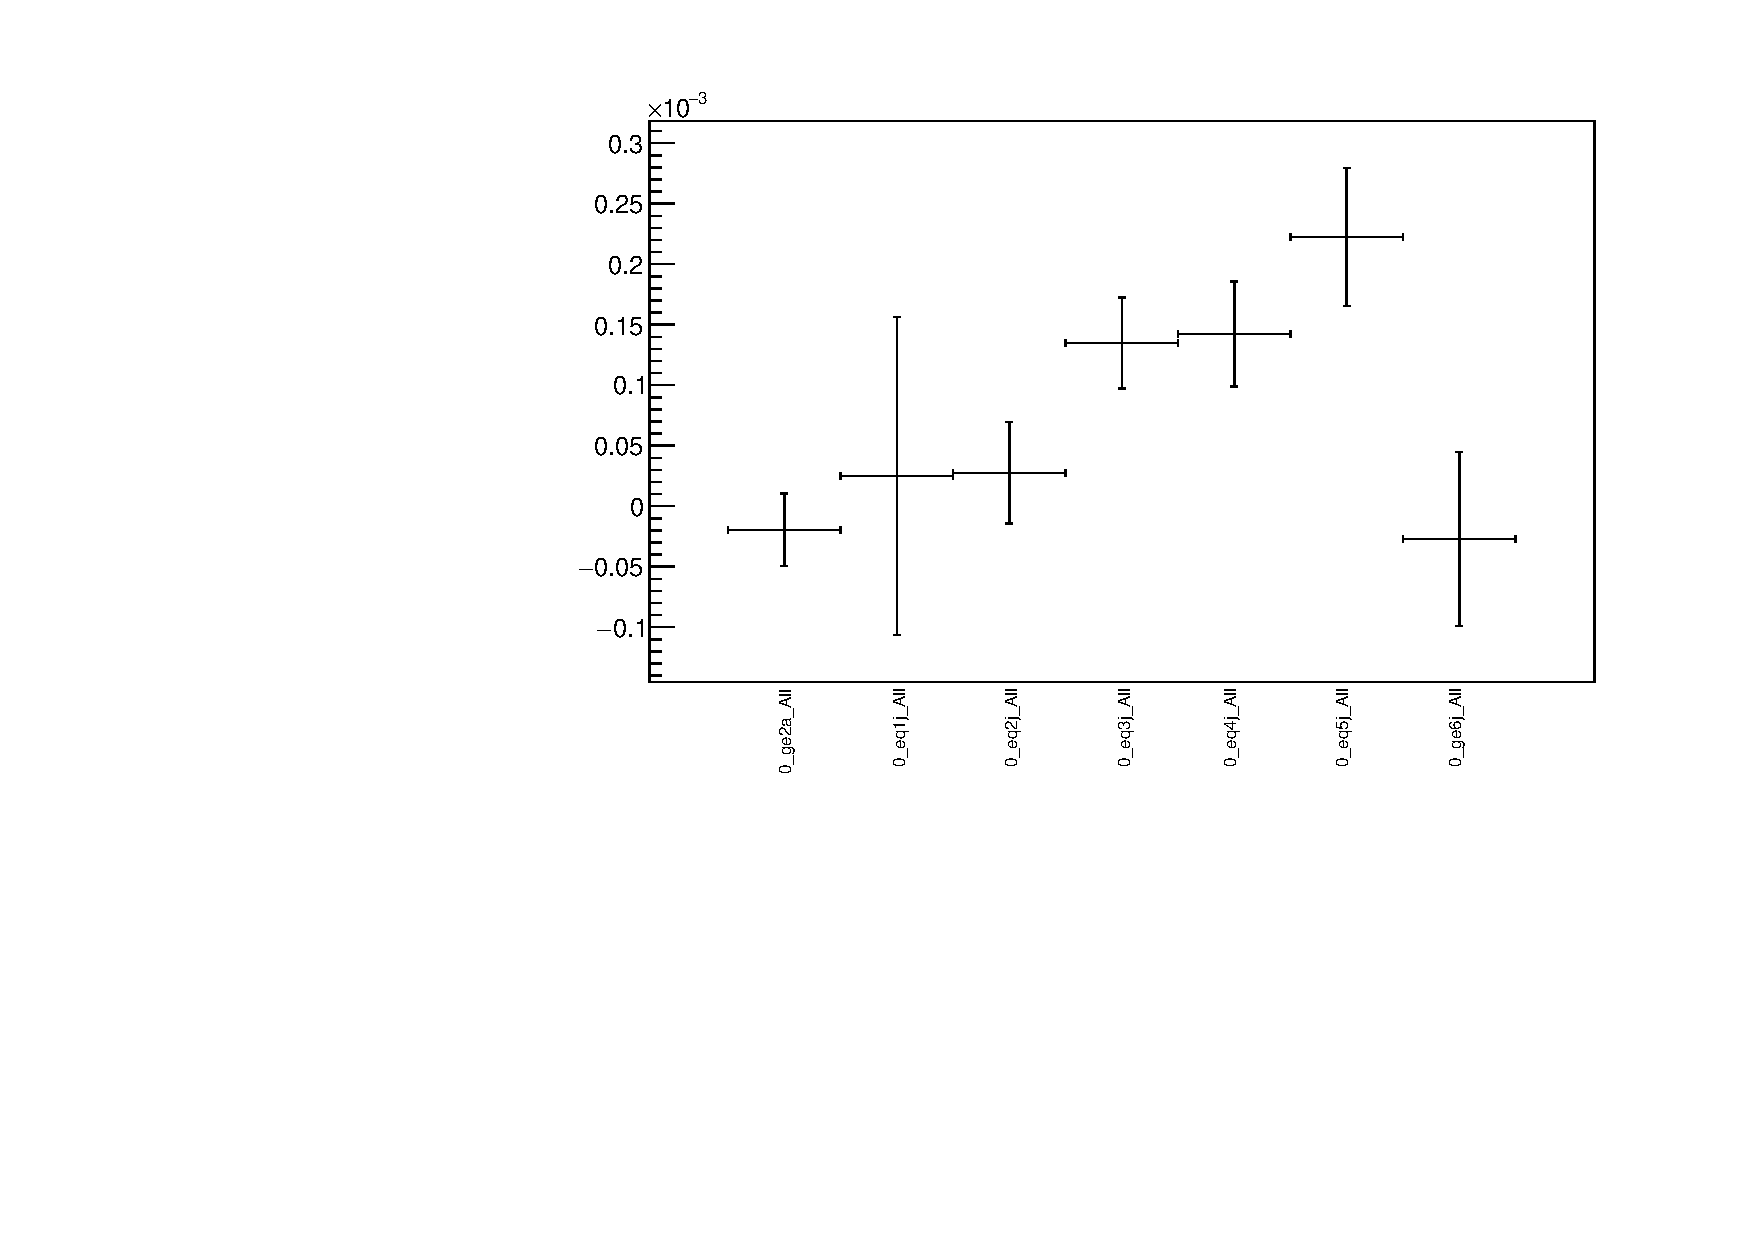
\includegraphics[width=0.5\textwidth]{figures/mhtTemplate/postFitValues/Mu_perNJet_graph.pdf}
  }~~
  \subfigure[\zInv~]{
    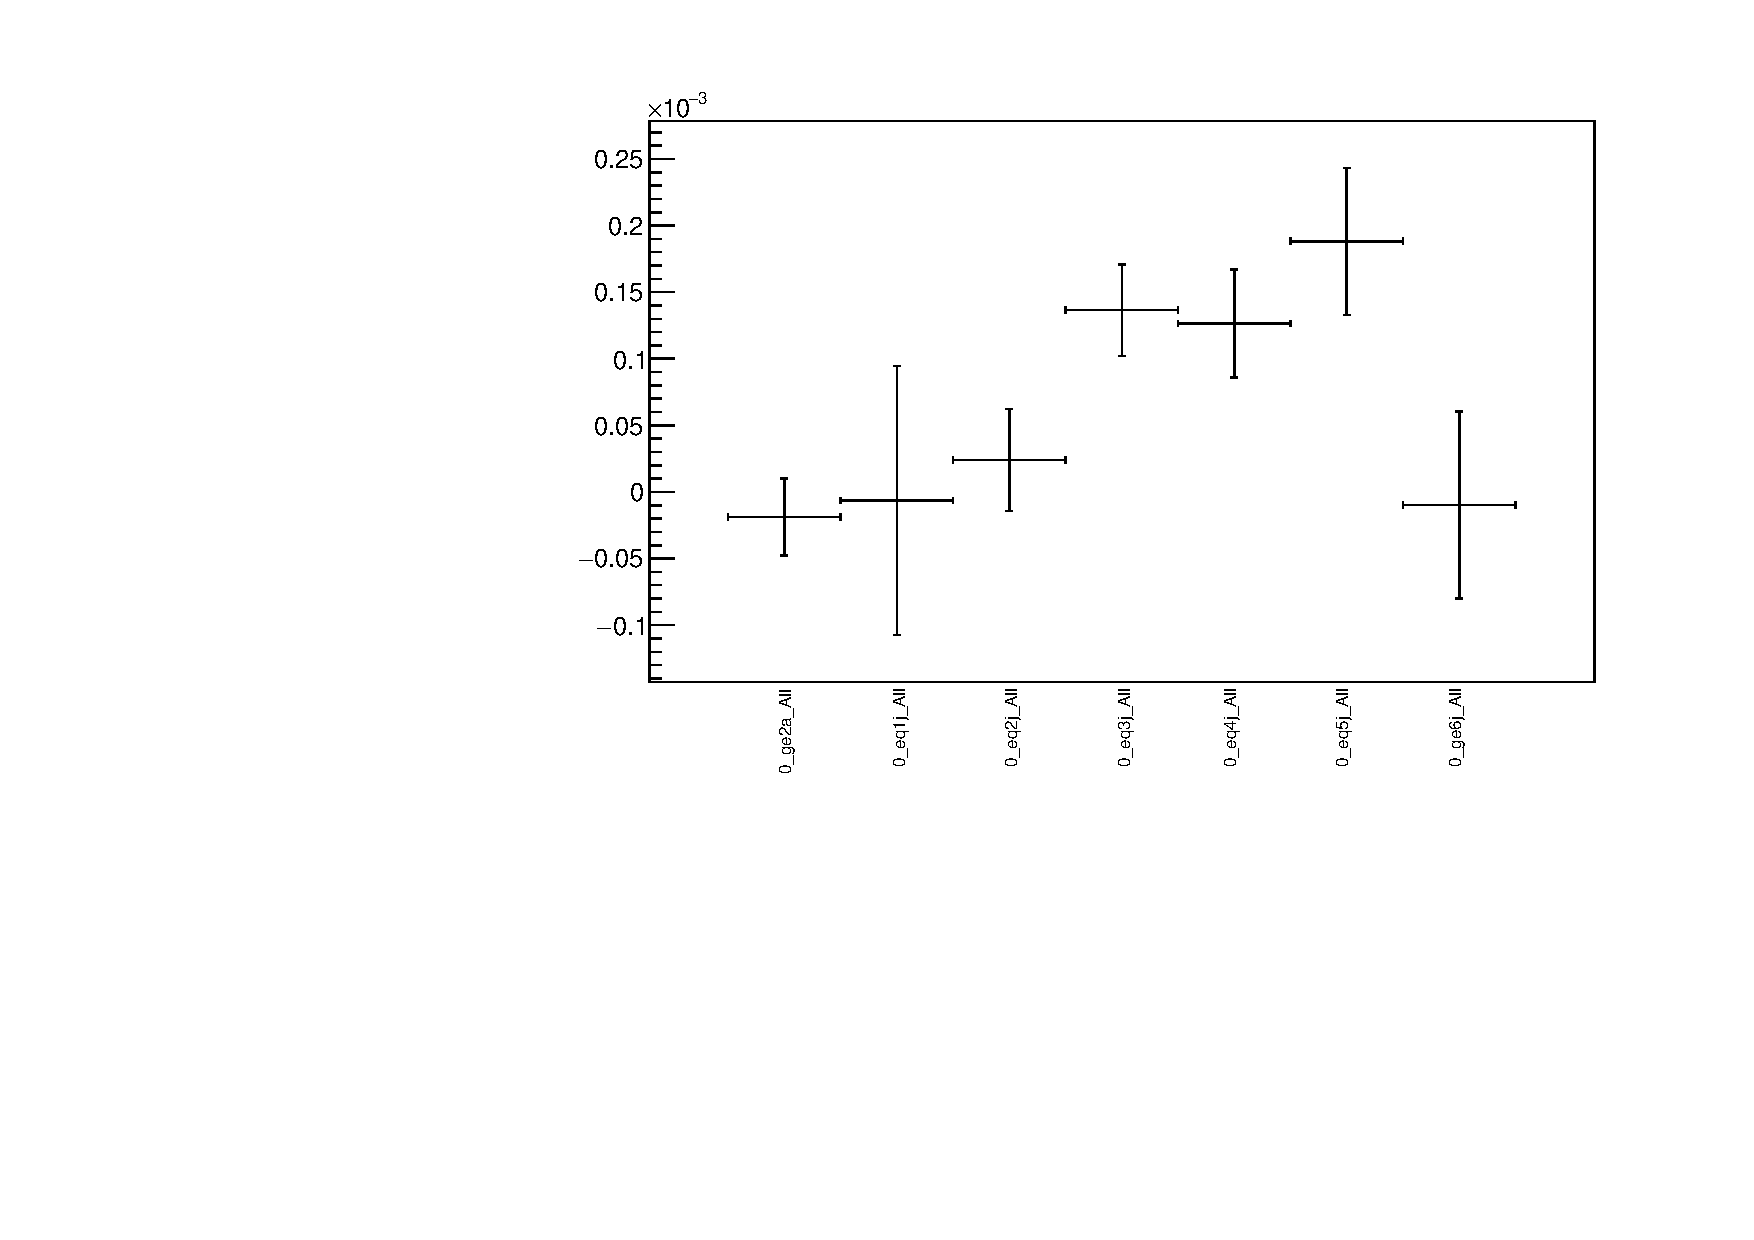
\includegraphics[width=0.5\textwidth]{figures/mhtTemplate/postFitValues/All_perNJet_graph.pdf}
  }\\
  \caption{\label{fig:postFitPerNJet} 
  Post fit values and uncertainties of the linear parameters used to determine the systematics decorrelated in \njet for 
  the \ttbar/W and \zInv~ predictions}
\end{figure}
\begin{figure}[h!]
  \centering
  \subfigure[\ttbar/W]{
    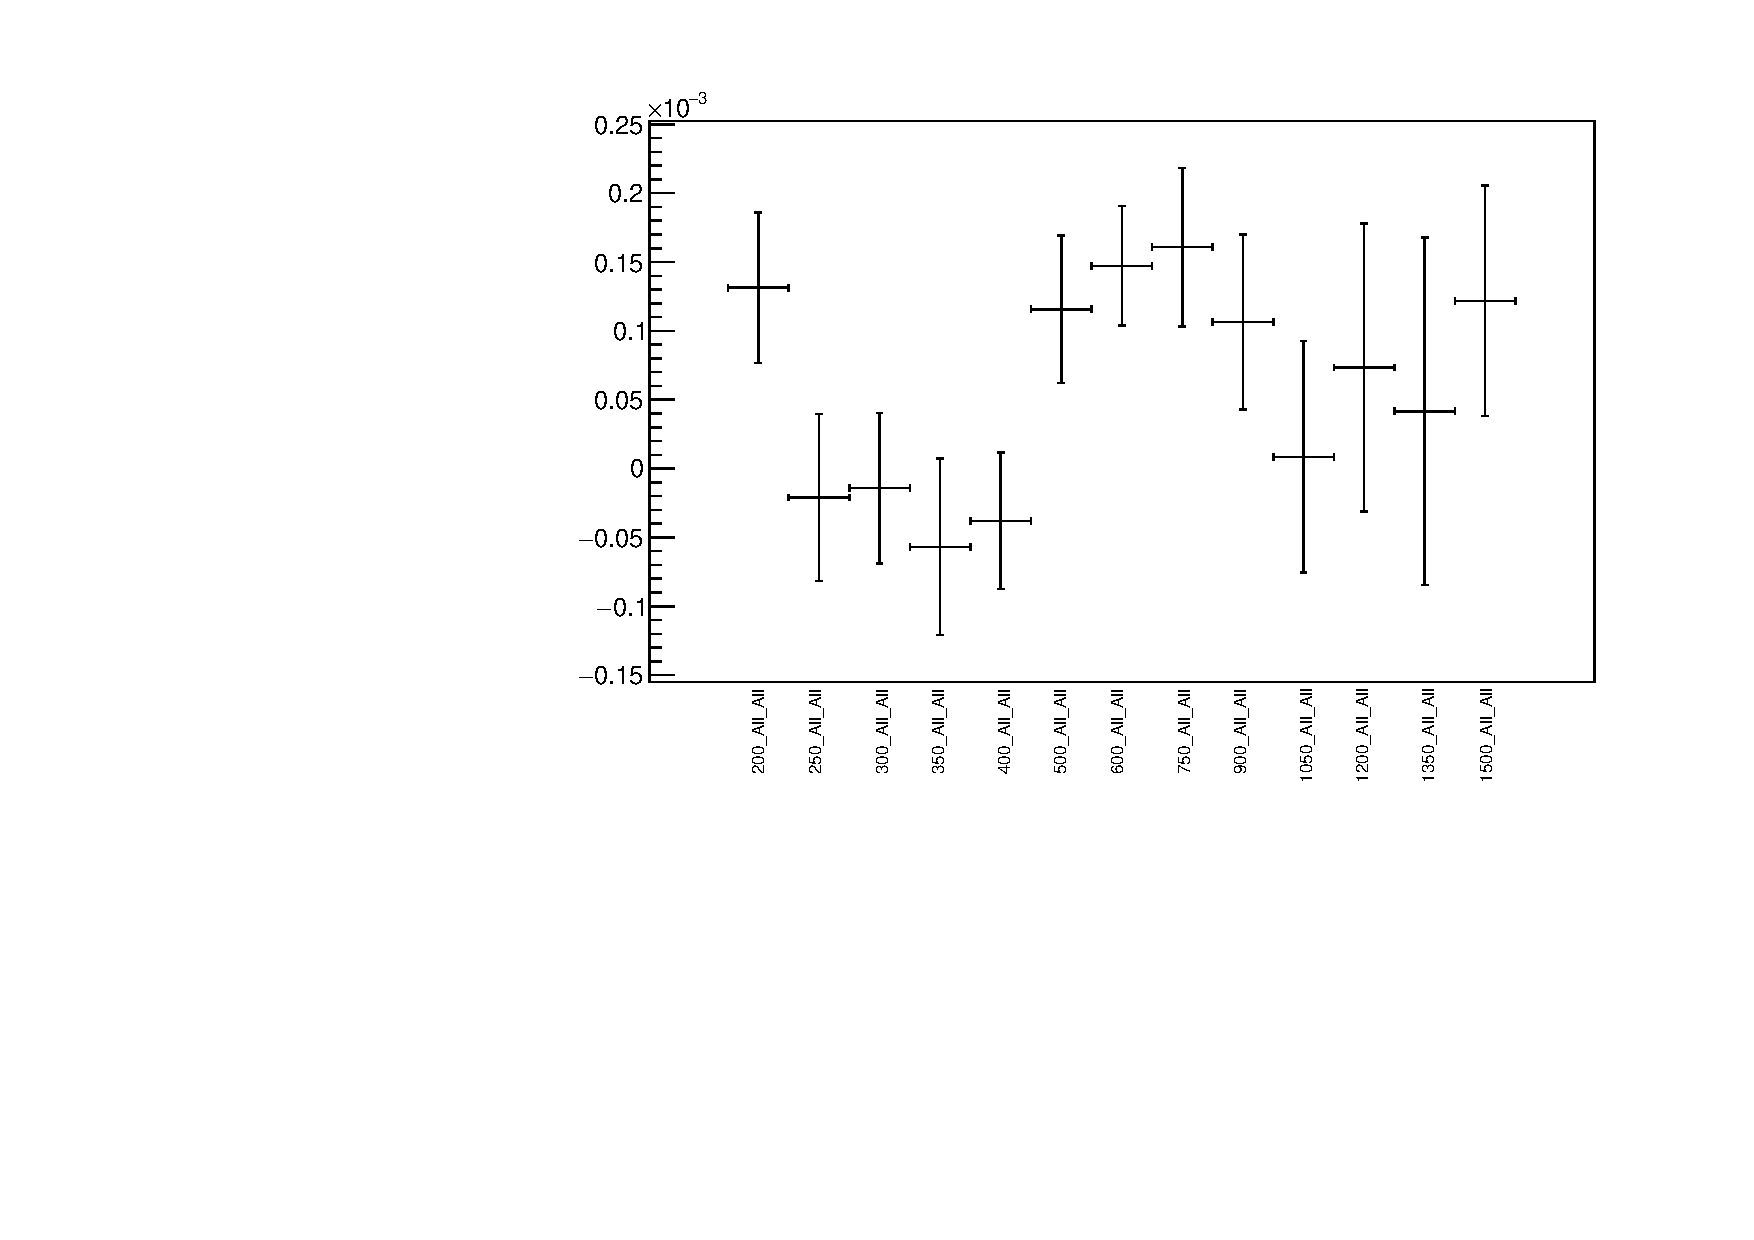
\includegraphics[width=0.5\textwidth]{figures/mhtTemplate/postFitValues/Mu_perHt_graph.pdf}
  }~~
  \subfigure[\zInv~]{
    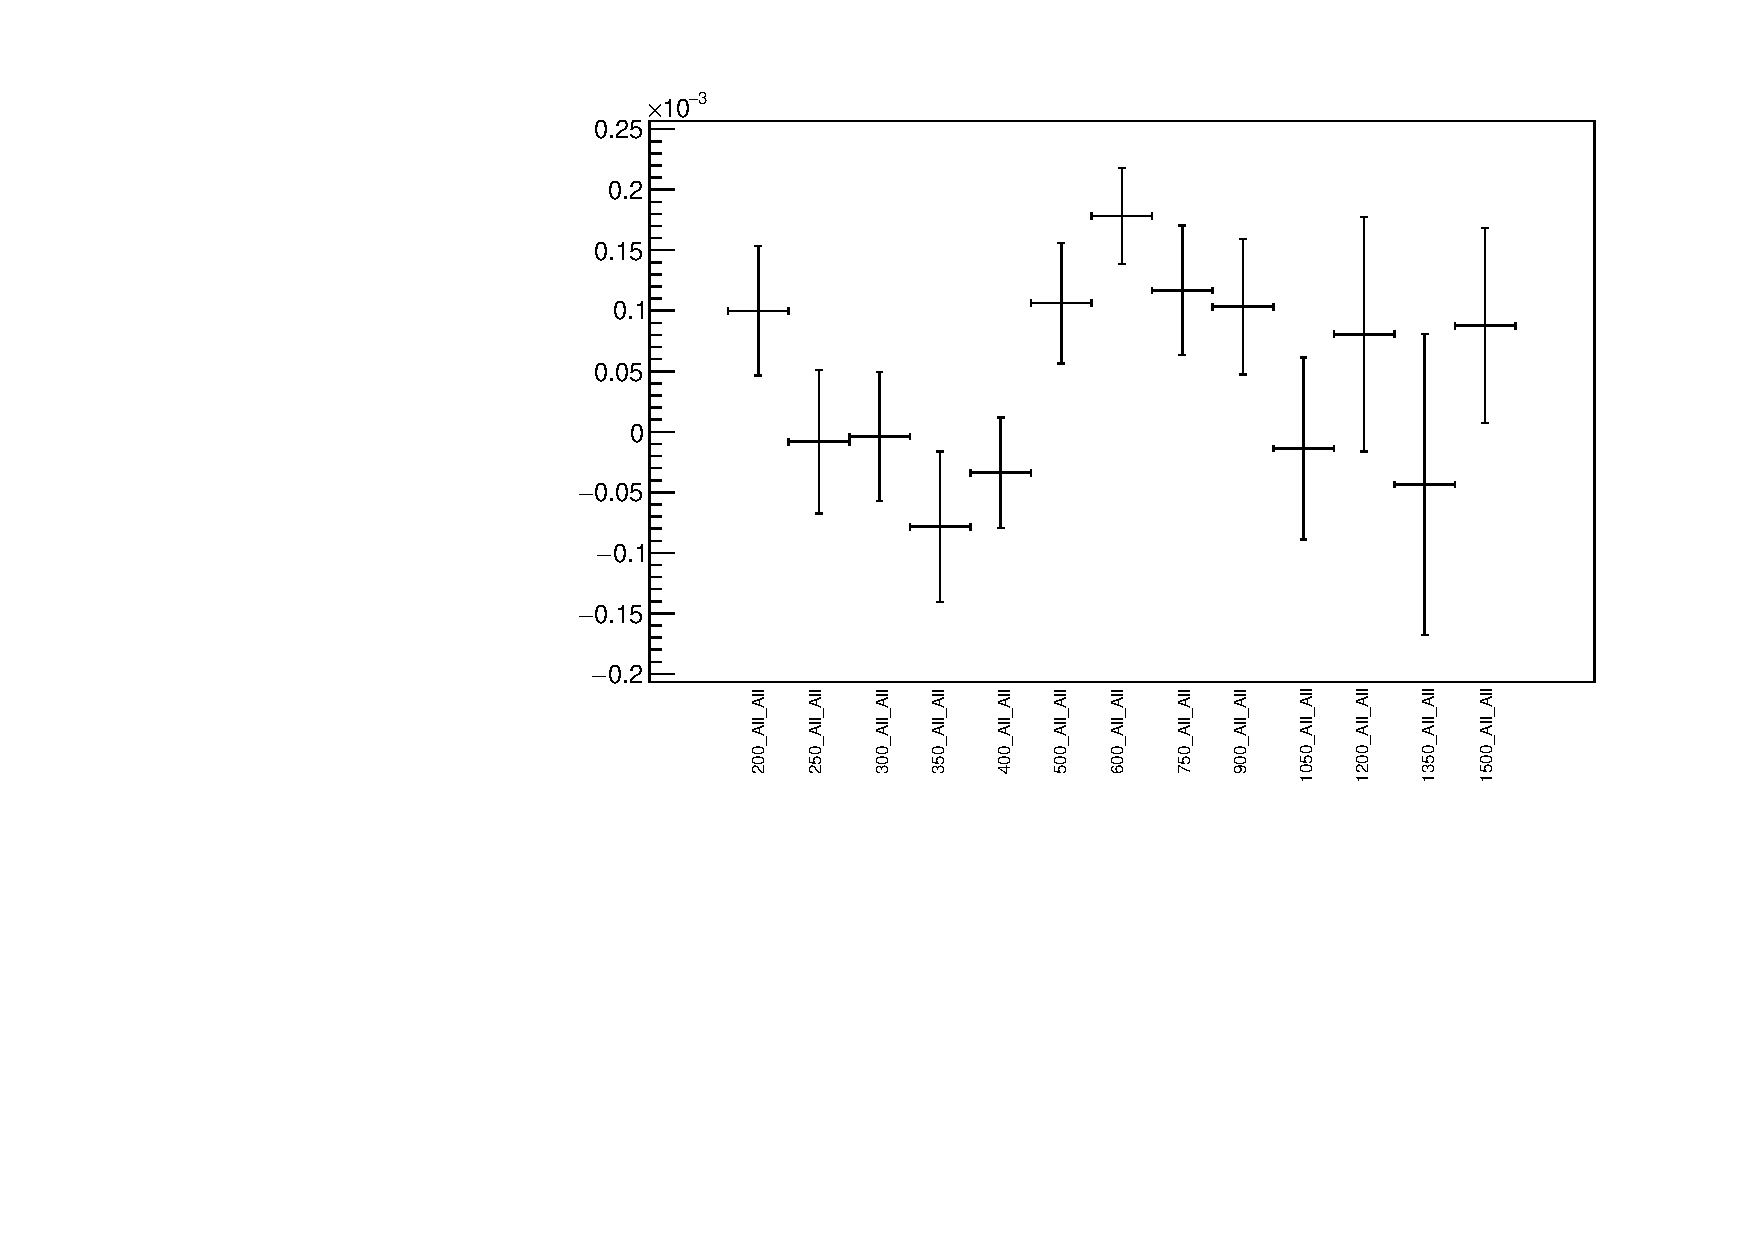
\includegraphics[width=0.5\textwidth]{figures/mhtTemplate/postFitValues/All_perHt_graph.pdf}
  }\\
  \caption{\label{fig:postFitPerHt} 
  Post fit values and uncertainties of the linear parameters used to determine the systematics decorrelated in \scalht for 
  the \ttbar/W and \zInv~ predictions}
\end{figure}
\begin{figure}[h!]
  \centering
  \subfigure[\ttbar/W]{
    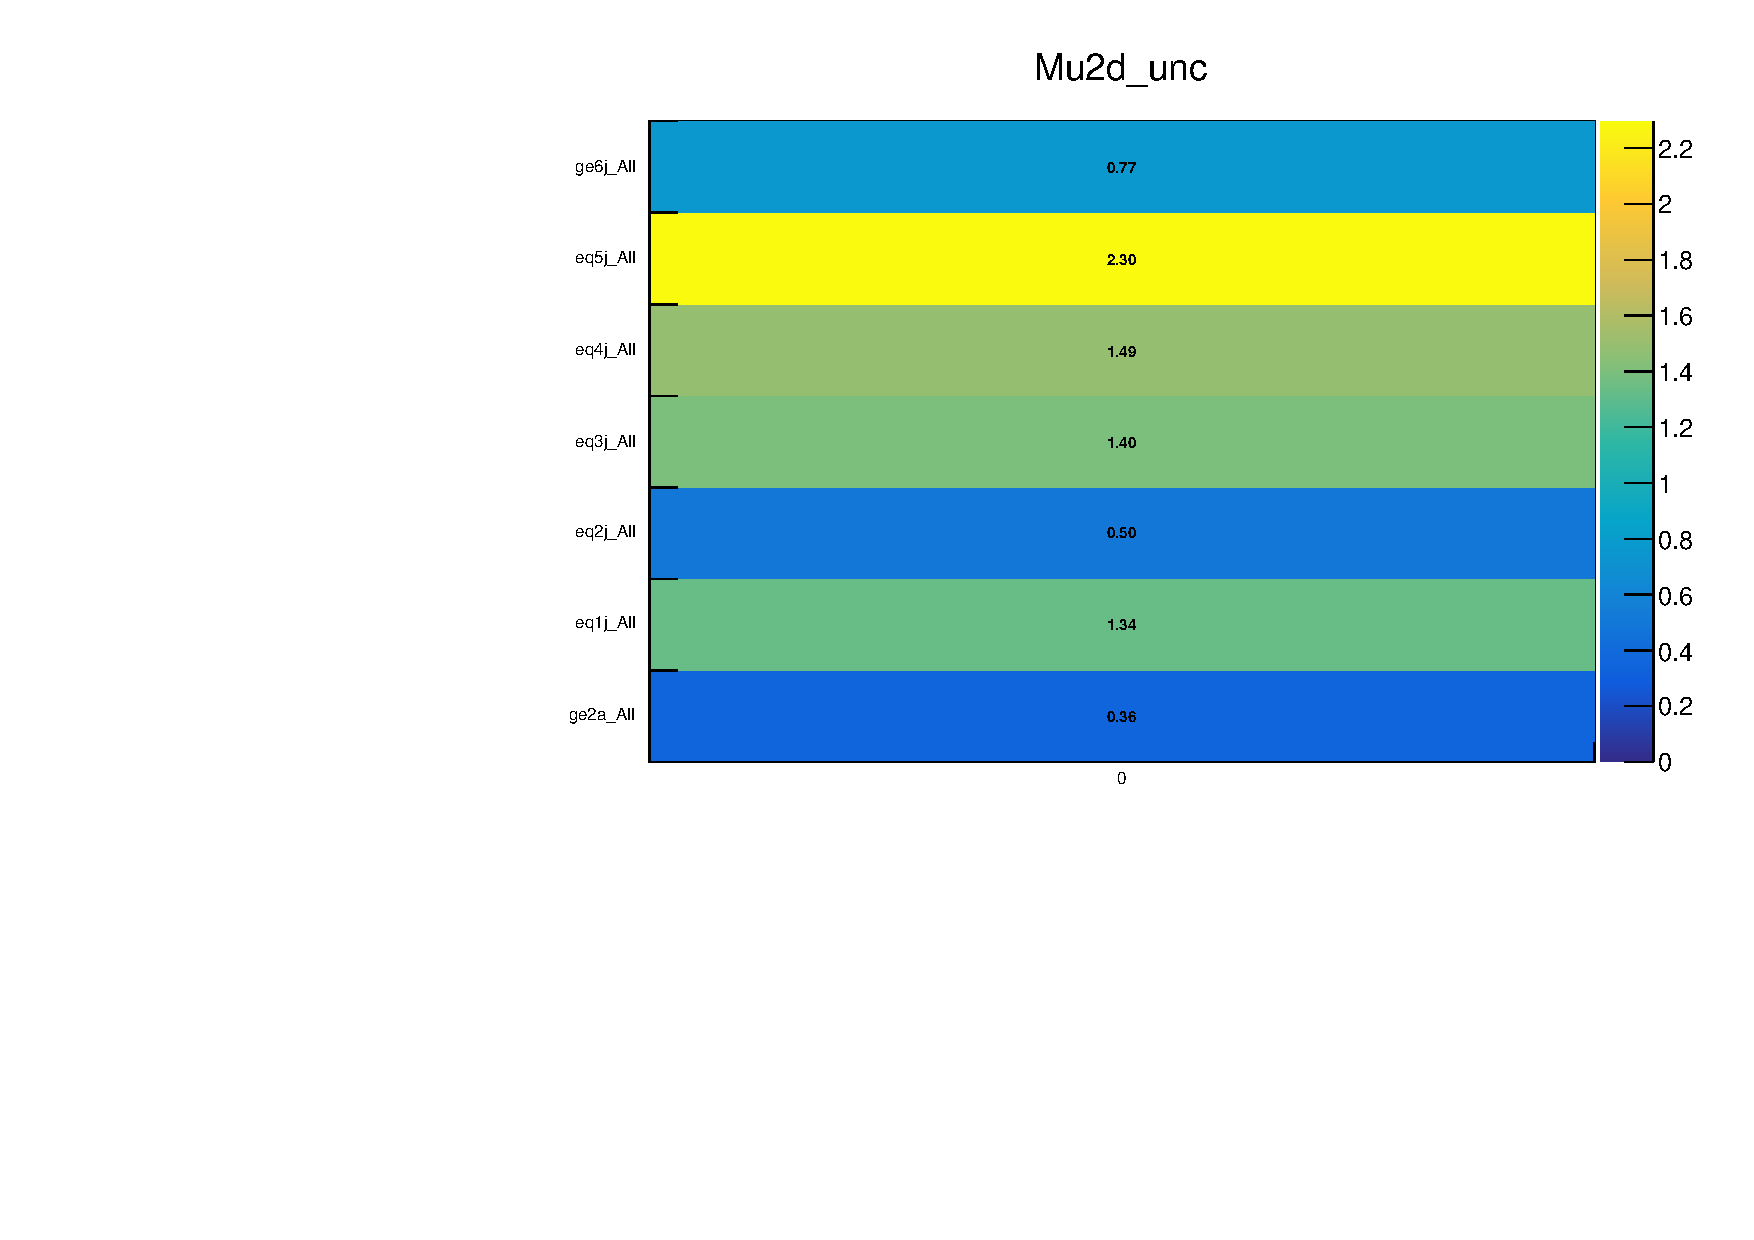
\includegraphics[width=0.5\textwidth]{figures/mhtTemplate/postFitValues/Mu_perNJet_unc.pdf}
  }~~
  \subfigure[\zInv~]{
    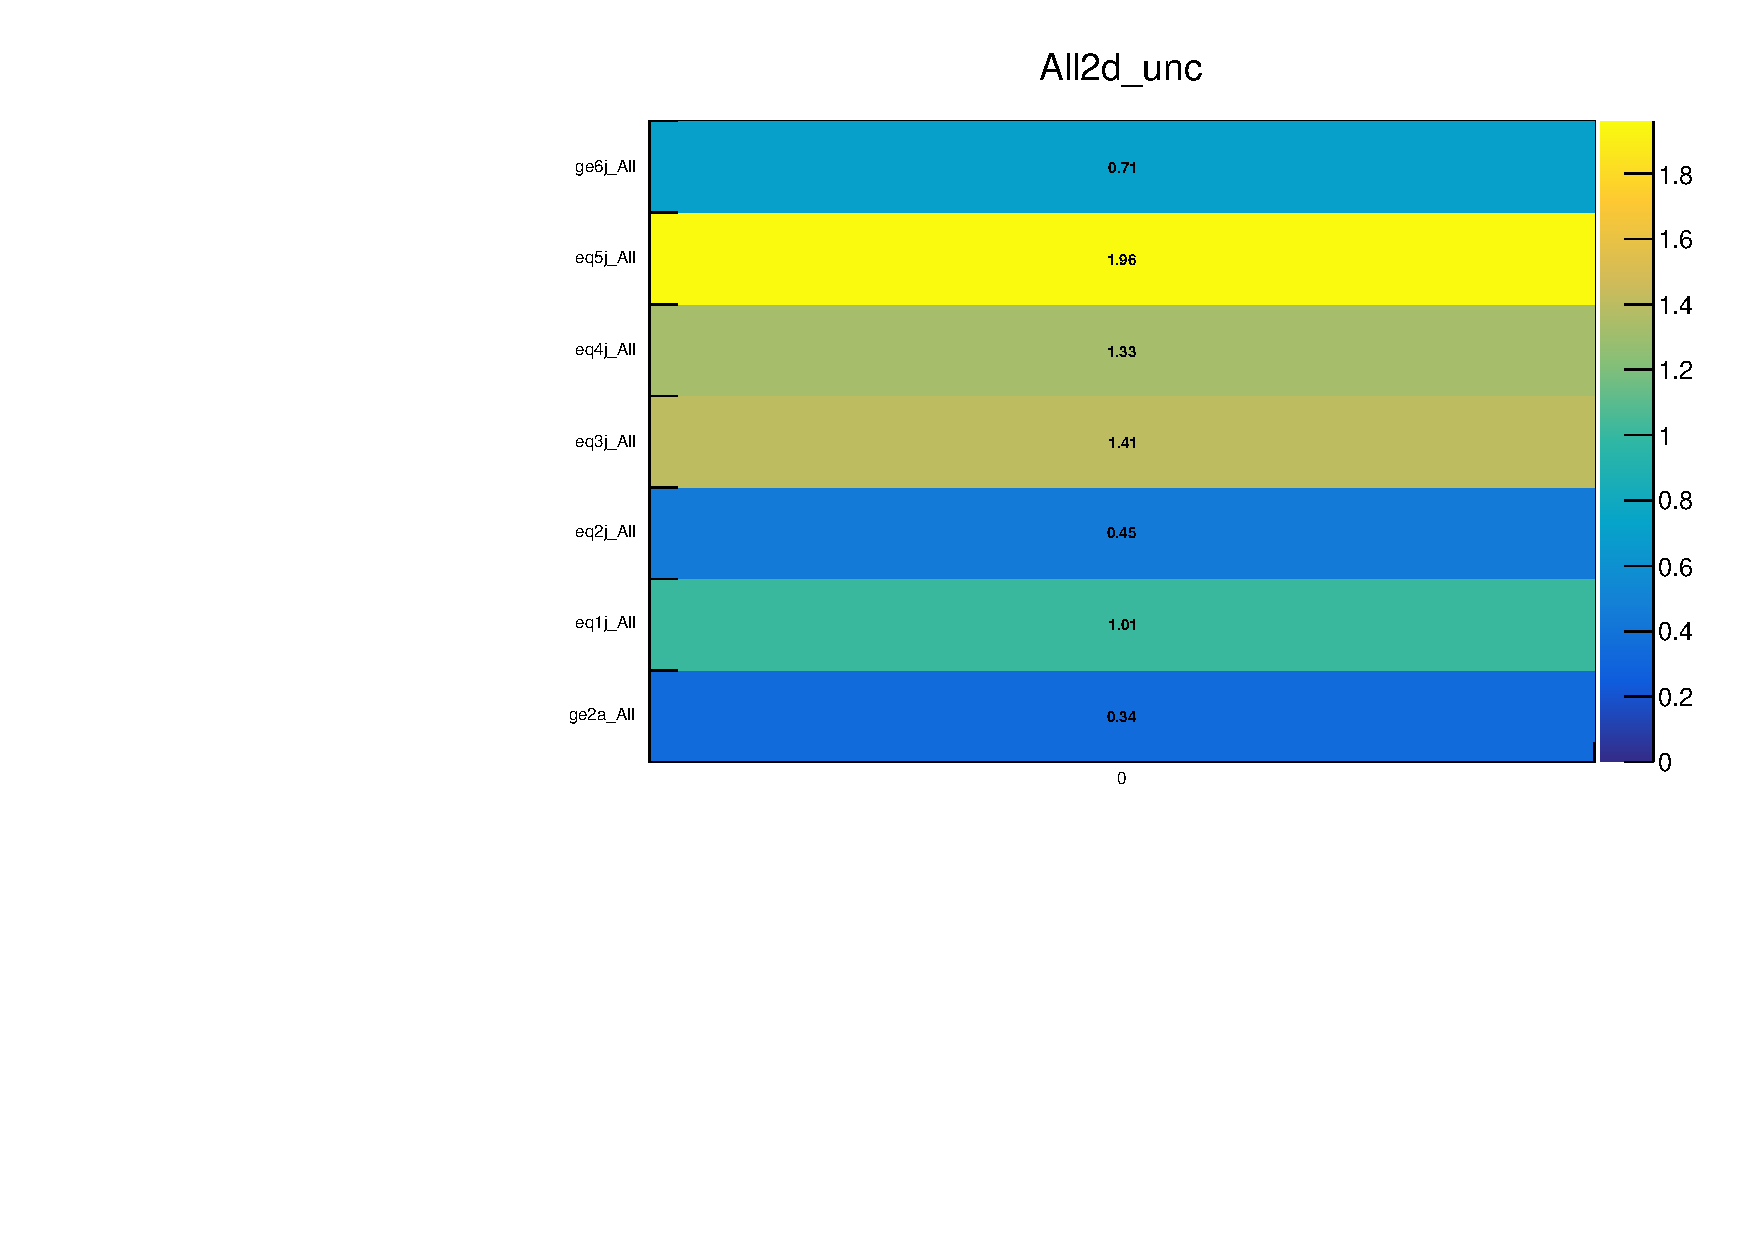
\includegraphics[width=0.5\textwidth]{figures/mhtTemplate/postFitValues/All_perNJet_unc.pdf}
  }\\
  \caption{\label{fig:uncPerNJet} 
     Percentage uncertainties per 100 GeV on the \mht distribution in the signal region for the systematics decorrelated in \njet
    for the \ttbar/W and \zInv~ predictions}
\end{figure}
\begin{figure}[h!]
  \centering
  \subfigure[\ttbar/W]{
    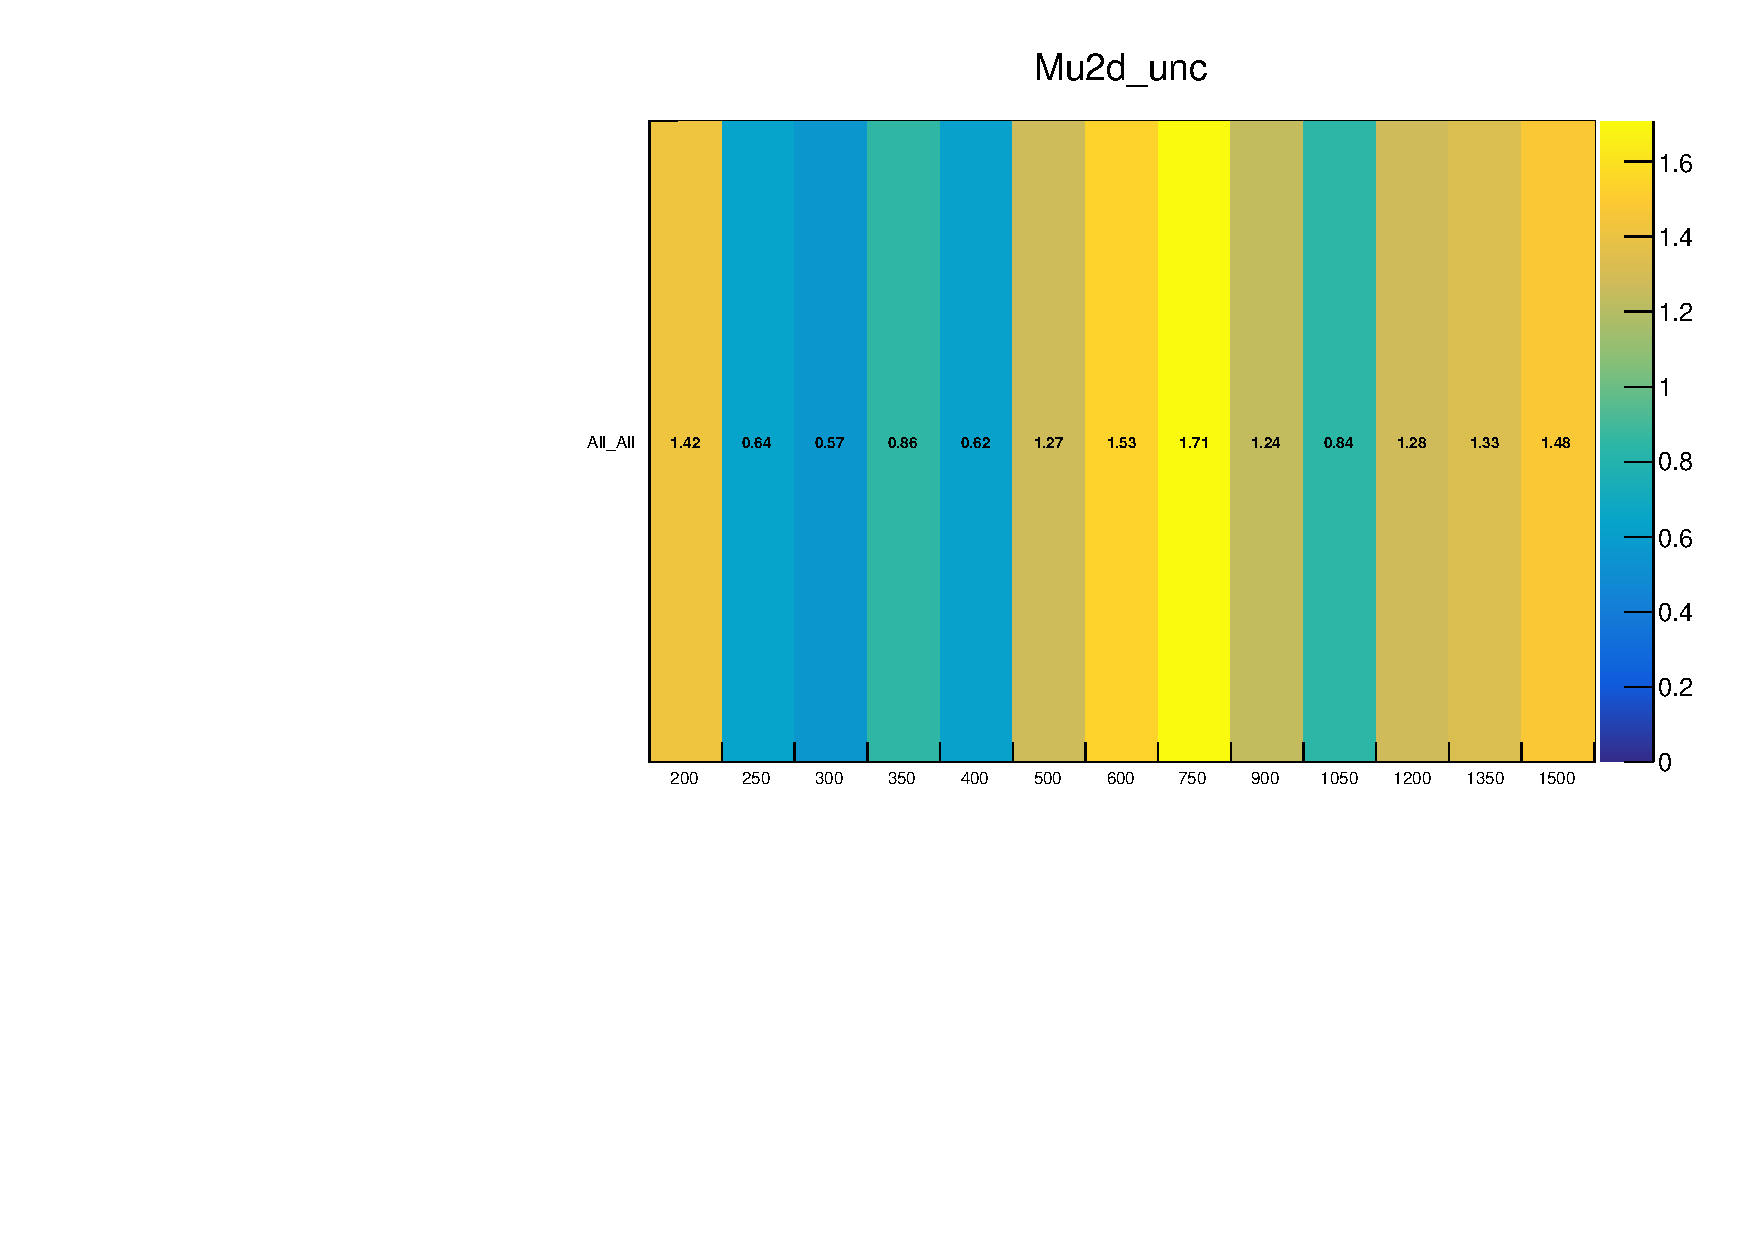
\includegraphics[width=0.5\textwidth]{figures/mhtTemplate/postFitValues/Mu_perHt_unc.pdf}
  }~~
  \subfigure[\zInv~]{
    \includegraphics[width=0.5\textwidth]{figures/mhtTemplate/postFitValues/All_perHt_unc.pdf}
  }\\
  \caption{\label{fig:uncPerHt} 
    Percentage uncertainties per 100 GeV on the \mht distribution in the signal region for the systematics decorrelated in \scalht
    for the \ttbar/W and \zInv~ predictions}
\end{figure}

\begin{figure}[h!]
  \centering
  \subfigure[\ttbar/W]{
    \includegraphics[width=0.5\textwidth]{figures/mhtTemplate/postFitValues/quadAddMu.pdf}
  }~~
  \subfigure[\zInv~]{
    \includegraphics[width=0.5\textwidth]{figures/mhtTemplate/postFitValues/quadAddAll.pdf}
  }\\
  \caption{\label{fig:frenchFlagLastBin} Observed percentage uncertainties in the 
  last bin of \mht over all categories and \scalht bins for the \ttbar/W and \zInv~ predictions.}
\end{figure}

\newpage
% \subsection{Comparison to known systematic sources}
% \label{sec:mcSystStudiesShape}
% To further validate the data driven procedure a range of known systematic sources are studied.
% The size of the variation of the \mht distribution under $\pm1\sigma$ shifts of these sources is compared 
% to that of the orthogonal polynomial systematic described in \ref{sec:valid13} to ensure they are
% covered. The sources considered are the b-tag scale factor uncertainty, jet energy correction uncertainty, 
% pile-up reweighting uncertainty, and top \Pt rewieghting uncertainty. For each source of systematic the prediction
% is varied by $\pm1\sigma$. To study the effect of this systematic variation on the \mht dimension, and not normalisation, 
% the resulting template is normalised to the nominal template in each jet category and \scalht bin. 
% These systematic effects can then be compared to the data-driven orthogonal polynomial systematic. 
%
% Figures~\ref{fig:mcCompLow} and \ref{fig:mcCompHigh} show the representative examples for two different \scalht 
% bins and jet-categories. As can be seen in each case the \mht dimension change under the variation of all 
% systematics considered is easily contained within the orthogonal polynomial variation. 
% To show the effect across all jet categories, except the monojet categories for which the \mht dimension is not used,
% and \scalht bins Fig~\ref{fig:lastBinVar} shows the maximum upwards/downwards variation in the last 
% \mht bin as a proportion of the orthogonal polynomial variation. In almost all bins this is shown to be 
% significantly less than unity confirming that the orthogonal polynomial can cover the known systematic
% deviations.
%
% \begin{figure}[h!]
%   \centering
%   \includegraphics[width=0.8\textwidth]{figures/template13TeV/mcComparison6fb/totalSMS-T1tttt_mGluino-1000_mLSP-100_25ns_mht_ge5j_ge3b_800.pdf}
%   \caption{\label{fig:mcCompLow} MC based systematic variations shown to be considerably smaller 
%   than the orthogonal polynomial data-driven systematic for an example bin \scalht $800-\infty$, \njet $\geq 5$, \nb $\geq 2$.}
% \end{figure}
% \begin{figure}[h!]
%   \centering
%   \includegraphics[width=0.8\textwidth]{figures/template13TeV/mcComparison6fb/totalSMS-T1tttt_mGluino-1000_mLSP-100_25ns_mht_eq2j_eq0b_400.pdf}
%   \caption{\label{fig:mcCompHigh} MC based systematic variations shown to be considerably smaller 
%   than the orthogonal polynomial data-driven systematic for an example bin \scalht 400-500, \njet $= 2$, \nb $= 0$.}
% \end{figure}
%
% \begin{figure}[h!]
% \centering
% \subfigure[Upwards deviation]{
% \includegraphics[width=0.5\textwidth]{figures/template13TeV/mcComparison6fb/lastBinRatioMax.pdf}
% }
% \subfigure[Downwards deviation]{
% \includegraphics[width=0.5\textwidth]{figures/template13TeV/mcComparison6fb/lastBinRatioMin.pdf}
% }\\
% \caption{\label{fig:lastBinVar} Maximum upwards and downwards variations in the last \mht bin as a proportion of the orthogonal polynomial deviation}
% \end{figure}

%%%____________________________________________________________________________||
\section{Likelihood model}
\label{sec:likelihood}

Consider a given category of event as defined by \njet, \nb~and \scalht, which are in the following identified with \htcat. 
In each category, the signal is extracted using the discriminating variable \mht. 
Histogram templates of the \mht distribution are built for the signal and the background processes 
using the MC samples described in Sec.~\ref{sec:datasets}. 
The \mht binning is tabulated in Sec.~\ref{sec:event-categorisation}.\\
The binning of the templates is chosen taking into account both the limited statistics in the simulation and 
the control of the background in data. 
%A maximum MC statistical uncertainty of 50\% (corresponding to 4 unweighted events) is required in each bin of the MC histogram template, 
%in order to ensure a statistically meaningful The uncertainty on the MC statistics in each bin is then 
taken into account with a dedicated nuisance parameter, one per template bin, as explained below. 
A minimum bin width constraint of 50 GeV is applied
in order to reduce the bin-by-bin migration due to the finite \mht resolution.\\

For each category \htcat and \mht bin, $i$, in the signal region, let $n^{\htcat}_{\mathrm{had},i}$ be the number of observed events, 
$b^{\htcat}_{\mathrm{had},i}$ the number of predicted background events and $s^{\htcat}_{\mathrm{had},i}$ the expected number of signal events. \\
The likelihood function for the hadronic signal region is, in each \htcat:

\begin{equation}
\mathcal{L}^{\htcat}_{\mathrm{had}}=\prod_i \mathrm{Poisson}(n^{\htcat}_{\mathrm{had},i} |\, b^{\htcat}_{\mathrm{had},i} + s^{\htcat}_{\mathrm{had},i})
\label{eq:hadronicLikelihood}
\end{equation}

The \mht dimension is not used for the control region, and they are used to constrain only the normalisation of the background processes 
in the signal region, as described in Sec.~\ref{sec:backgroundmet}. 
Their likelihood is therefore written as:

\begin{equation}
\mathcal{L}^{\htcat}_{\mathrm{CR,j}}=\mathrm{Pois}(n^{\htcat}_{\mathrm{CR,j}} |\, b^{\htcat}_{\mathrm{CR,j}} + s^{\htcat}_{\mathrm{CR,j}})
\label{eq:controlLikelihood}
\end{equation}

In Eq.~\ref{eq:controlLikelihood}, $n^{\htcat}_{\mathrm{CR,j}}$ is the number of observed events, $b^{\htcat}_{\mathrm{CR,j}}$ the number of predicted 
background events and $s^{\htcat}_{\mathrm{CR,j}}$ the expected number of signal events in the control region $j$. \\
Eq.~\ref{eq:controlLikelihood} applies to all the control region used for the background estimation, 
as defined in Sec.~\ref{sec:selection}. \\
Notice that the signal contribution $s^{\htcat}_{\mathrm{CR,j}}$ in Eq.~\ref{eq:controlLikelihood}, as estimated from MC, is in general negligible. 
Where the signal contamination is sizeable, it is included in the likelihood as an additional process contributing to the event yield in that particular bin.

The prediction of the background yields in the signal region and in the corresponding control samples are connected 
by means of transfer factors, as explained in Sec.~\ref{sec:backgroundmet}. 
This connection is implemented by introducing a floating parameter, which is correlated 
between the signal region and the control regions. 
One floating parameter is used for both background 
processes ($Z_{\mathrm{inv.}}$ and \ttbar/W) \footnote{In the following we use $Z_{\mathrm{inv}}$ to indicate 
the $Z\to \mathrm{inv}$ process and \ttbar/W to indicate the sum of the yields of the $t\bar{t}$ and $W+\mathrm{jets}$ processes.}
giving a prediction for each background source depending on the relevant nuisances described below. \\
This binds the background yields in the signal and control regions to float together, 
taking into account the statistical uncertainty associated with the counts in the control samples. 

The systematic uncertainties affecting the transfer factors, described in Sec.~\ref{sec:systematics}, 
are incorporated in the likelihood by means of nuisance parameters with gaussian constraints which act on the floating
parameter. These depend on the background process and the control region used for the prediction and
are taken as uncorrelated between each of the \htcat bins. Additionally, systematic effects studied 
through variations in simulation, like b-tag SF and jet energy corrections, are included as shape uncertainties on the transfer factors. 
The are taken as fully correlated across all bins but have different sizes depending on the bin. The effects 
of these systematics are determined using the method described in Sec~\ref{sec:systematics}. \\
The uncertainties on the signal efficiency times acceptance, described in Sec.~\ref{sec:susy}, 
are also taken as shape uncertainties correlated across all the \htcat bins. 
The uncertainty that encapsulates the potential for bin migration within the \mht distribution of events is implemented 
providing alternative templates corresponding to up/down variation of each source, separately for each \htcat bin. 
The procedure to assess the alternative templates is described in detail in Sec.~\ref{sec:syst-on-shape}. \\
The uncertainty due to the limited statistics in the MC samples used to populate the template histograms is incorporated 
as additional nuisance parameters, one per template bin, taken as uncorrelated across the histogram bins. 

The total likelihood is the product over all the \htcat bins and all the control regions, and can be written as:

\begin{equation}
\label{eq:total_likelihood}
\mathcal{L} = \prod_{\htcat} \mathcal{L}_{\text{had}}^{\htcat} \times \prod_{\text{j}} \mathcal{L}_{\text{CR,j}}^{\htcat}
\end{equation}

The fit is carried out in two steps. 
In the first, the background predictions for the signal region $b^{\htcat}_{\mathrm{had},i}$ are extracted from a likelihood fit 
using the control regions in Eq.~\ref{eq:controlLikelihood} without the signal region. 
This fit provides the best knowledge of the background yields in the signal region, 
and the predictions can therefore be used to re-interpret the analysis. 
In the second step, the fit is done using the full likelihood (Eq.~\ref{eq:total_likelihood}) and all 
the correlations between the backgrounds in control regions and signal region are taken into account, 
together with the statistical uncertainty associated to the finite number of events in the control region. \\
The likelihood is profiled against all nuisance parameters in order to derive expected exclusion limits and sensitivity, 
which will be discussed in Sec.\ref{sec:susy}, \ref{sec:darkmatter}.

%For technical limitations, only a subset of jet multiplicity categories are combined to derive the exclusion limits. 
%Four out of nine \nj\ categories are included, while considering all the \nb, \scalht, \mht bins within each \nj category. 
%These four categories are chosen as the ones providing the best expected exclusion for each signal point separately. \\
%% In App.~\ref{app:jetRanking}, the details of this ranking are given for all the models considered in the analysis. 
%% The four categories used in the limits are also shown in tabular format for some benchmark models in Tab.~\ref{tab:sig-eff-bestCat}.




%%____________________________________________________________________________||

%\include{140_results}
%\include{150_susy}
%%\include{160_darkmatter}
%%%____________________________________________________________________________||
\section{Results}
\label{sec:results}

\fixme{To come.}

%%____________________________________________________________________________||
\section{Interpretation in Simplified SUSY models}
\label{sec:susy}

\fixme{To come.}

%%__________________________________________________________________||
\section{Summary}
\label{sec:summary}

\fixme{To come.}

%An inclusive search for supersymmetry with the CMS experiment is
%reported, based on a data sample of pp collisions collected at
%$\sqrt{s} = 13\TeV$, corresponding to an integrated luminosity of $36.4\, \fbinv$. 
%Final states with jets and significant \met, as
%expected from the production and decay of massive squarks and gluinos,
%have been analysed.  The signal region is binned according to the
%number of reconstructed jets, the scalar and vector sums of the
%transverse energy of jets, and the number of jets identified to
%originate from bottom quarks. 
%Multiple control regions in data have been used to estimate the standard model background in 
%the signal region. 
%%The observed yields in the signal region are found to be in agreement with
%the expected contributions from standard model processes. \\
%% Limits are determined in the mass parameter space of simplified models 
%% involving the gluino-mediated and direct production of squark pairs. 
%% The excluded mass parameter space extends significantly beyond that 
%% set by previous searches, with observed exclusions in gluino mass, 
%% and light-flavour, bottom, and top squark masses, as high as 1775, 
%% 1425, 1025, and 875 GeV, respectively.

%%__________________________________________________________________||


%%____________________________________________________________________________||

\bibliography{auto_generated}

%%____________________________________________________________________________||

\appendix
%%____________________________________________________________________________||
\section{Data sets and simulation}
\label{app:datasets}

\begin{table}[h!]
  \topcaption{List of primary data sets used in this analysis.}
  \footnotesize 
  \begin{center}
\begin{tabular}{l}
\hline\hline
\multicolumn{1}{c}{Data set}\tabularnewline
\hline
\verb!/HTMHT/Run2016B-23Sep2016-v3/MINIAOD!\tabularnewline
\verb!/HTMHT/Run2016C-23Sep2016-v1/MINIAOD!\tabularnewline
\verb!/HTMHT/Run2016D-23Sep2016-v1/MINIAOD!\tabularnewline
\verb!/HTMHT/Run2016E-23Sep2016-v1/MINIAOD!\tabularnewline
\verb!/HTMHT/Run2016F-23Sep2016-v1/MINIAOD!\tabularnewline
\verb!/HTMHT/Run2016G-23Sep2016-v2/MINIAOD!\tabularnewline
\verb!/HTMHT/Run2016H-PromptReco-v2/MINIAOD!\tabularnewline
\verb!/HTMHT/Run2016H-PromptReco-v3/MINIAOD!\tabularnewline
\verb!/JetHT/Run2016B-23Sep2016-v2/MINIAOD!\tabularnewline
\verb!/JetHT/Run2016C-23Sep2016-v2/MINIAOD!\tabularnewline
\verb!/JetHT/Run2016D-23Sep2016-v2/MINIAOD!\tabularnewline
\verb!/JetHT/Run2016E-23Sep2016-v1/MINIAOD!\tabularnewline
\verb!/JetHT/Run2016F-23Sep2016-v1/MINIAOD!\tabularnewline
\verb!/JetHT/Run2016G-23Sep2016-v2/MINIAOD!\tabularnewline
\verb!/JetHT/Run2016H-PromptReco-v2/MINIAOD!\tabularnewline
\verb!/JetHT/Run2016H-PromptReco-v3/MINIAOD!\tabularnewline
\verb!/MET/Run2016B-23Sep2016-v3/MINIAOD!\tabularnewline
\verb!/MET/Run2016C-23Sep2016-v1/MINIAOD!\tabularnewline
\verb!/MET/Run2016D-23Sep2016-v1/MINIAOD!\tabularnewline
\verb!/MET/Run2016E-23Sep2016-v1/MINIAOD!\tabularnewline
\verb!/MET/Run2016F-23Sep2016-v1/MINIAOD!\tabularnewline
\verb!/MET/Run2016G-23Sep2016-v1/MINIAOD!\tabularnewline
\verb!/MET/Run2016H-PromptReco-v2/MINIAOD!\tabularnewline
\verb!/SingleMuon/Run2016B-23Sep2016-v3/MINIAOD!\tabularnewline
\verb!/SingleMuon/Run2016C-23Sep2016-v1/MINIAOD!\tabularnewline
\verb!/SingleMuon/Run2016D-23Sep2016-v1/MINIAOD!\tabularnewline
\verb!/SingleMuon/Run2016E-23Sep2016-v1/MINIAOD!\tabularnewline
\verb!/SingleMuon/Run2016F-23Sep2016-v1/MINIAOD!\tabularnewline
\verb!/SingleMuon/Run2016G-23Sep2016-v1/MINIAOD!\tabularnewline
\verb!/SingleMuon/Run2016H-PromptReco-v2/MINIAOD!\tabularnewline
\verb!/SingleMuon/Run2016H-PromptReco-v3/MINIAOD!\tabularnewline
\verb!/SinglePhoton/Run2016B-23Sep2016-v3/MINIAOD!\tabularnewline
\verb!/SinglePhoton/Run2016C-23Sep2016-v1/MINIAOD!\tabularnewline
\verb!/SinglePhoton/Run2016D-23Sep2016-v1/MINIAOD!\tabularnewline
\verb!/SinglePhoton/Run2016E-23Sep2016-v1/MINIAOD!\tabularnewline
\verb!/SinglePhoton/Run2016F-23Sep2016-v1/MINIAOD!\tabularnewline
\verb!/SinglePhoton/Run2016G-23Sep2016-v1/MINIAOD!\tabularnewline
\verb!/SinglePhoton/Run2016H-PromptReco-v2/MINIAOD!\tabularnewline
\verb!/SinglePhoton/Run2016H-PromptReco-v3/MINIAOD!\tabularnewline
\verb!/DoubleEG/Run2016B-23Sep2016-v3/MINIAOD!\tabularnewline
\verb!/DoubleEG/Run2016C-23Sep2016-v1/MINIAOD!\tabularnewline
\verb!/DoubleEG/Run2016D-23Sep2016-v1/MINIAOD!\tabularnewline
\verb!/DoubleEG/Run2016E-23Sep2016-v1/MINIAOD!\tabularnewline
\verb!/DoubleEG/Run2016F-23Sep2016-v1/MINIAOD!\tabularnewline
\verb!/DoubleEG/Run2016G-23Sep2016-v1/MINIAOD!\tabularnewline
\verb!/DoubleEG/Run2016H-PromptReco-v2/MINIAOD!\tabularnewline
\verb!/DoubleEG/Run2016H-PromptReco-v3/MINIAOD!\tabularnewline
\hline
\end{tabular}\end{center}

  \label{tab:datasets_data}
\end{table}

\begin{table}[h!]
  \centering
  \topcaption{Simulated event samples of SM background processes used
    by this analysis. Symbols used as shorthand are defined at the
    bottom of the table.
    Other samples are described in Table~\ref{tab:datasets_bkg2}}
  \fontsize{7}{8.4}\selectfont
  %latex.default(d, title = NULL, booktabs = FALSE, width = 3, rowname = NULL,     helvetica = FALSE, caption.loc = "bottom", ...)%
\begin{center}
\begin{tabular}{ll}
\hline\hline
\multicolumn{1}{c}{Data set}&\multicolumn{1}{c}{Cross section [pb]}\tabularnewline
\hline
\verb!/ZJetsToNuNu_HT-100To200_13TeV-madgraph/[1]-v1/MINIAODSIM! &$3.448\times 10^{+02}$\tabularnewline
\verb!/ZJetsToNuNu_HT-100To200_13TeV-madgraph/[1]_ext1-v1/MINIAODSIM! &$3.448\times 10^{+02}$\tabularnewline
\verb!/ZJetsToNuNu_HT-200To400_13TeV-madgraph/[1]-v1/MINIAODSIM! &$9.553\times 10^{+01}$\tabularnewline
\verb!/ZJetsToNuNu_HT-200To400_13TeV-madgraph/[1]_ext1-v1/MINIAODSIM! &$9.553\times 10^{+01}$\tabularnewline
\verb!/ZJetsToNuNu_HT-400To600_13TeV-madgraph/[1]-v1/MINIAODSIM! &$1.320\times 10^{+01}$\tabularnewline
\verb!/ZJetsToNuNu_HT-400To600_13TeV-madgraph/[1]_ext1-v1/MINIAODSIM! &$1.320\times 10^{+01}$\tabularnewline
\verb!/ZJetsToNuNu_HT-600To800_13TeV-madgraph/[1]-v1/MINIAODSIM! &$3.221\times 10^{+00}$\tabularnewline
\verb!/ZJetsToNuNu_HT-800To1200_13TeV-madgraph/[1]-v1/MINIAODSIM! &$1.474\times 10^{+00}$\tabularnewline
\verb!/ZJetsToNuNu_HT-1200To2500_13TeV-madgraph/[1]-v1/MINIAODSIM! &$3.586\times 10^{-01}$\tabularnewline
\verb!/ZJetsToNuNu_HT-1200To2500_13TeV-madgraph/[1]_ext1-v1/MINIAODSIM! &$3.586\times 10^{-01}$\tabularnewline
\verb!/ZJetsToNuNu_HT-2500ToInf_13TeV-madgraph/[1]-v1/MINIAODSIM! &$8.203\times 10^{-03}$\tabularnewline
\verb!/WJetsToLNu_HT-100To200_[2]/[1]-v1/MINIAODSIM! &$1.627\times 10^{+03}$\tabularnewline
\verb!/WJetsToLNu_HT-100To200_[2]/[1]_ext1-v1/MINIAODSIM! &$1.627\times 10^{+03}$\tabularnewline
\verb!/WJetsToLNu_HT-100To200_[2]/[1]_ext2-v1/MINIAODSIM! &$1.627\times 10^{+03}$\tabularnewline
\verb!/WJetsToLNu_HT-200To400_[2]/[1]-v1/MINIAODSIM! &$4.352\times 10^{+02}$\tabularnewline
\verb!/WJetsToLNu_HT-200To400_[2]/[1]_ext1-v1/MINIAODSIM! &$4.352\times 10^{+02}$\tabularnewline
\verb!/WJetsToLNu_HT-200To400_[2]/[1]_ext2-v1/MINIAODSIM! &$4.352\times 10^{+02}$\tabularnewline
\verb!/WJetsToLNu_HT-400To600_[2]/[1]-v1/MINIAODSIM! &$5.918\times 10^{+01}$\tabularnewline
\verb!/WJetsToLNu_HT-400To600_[2]/[1]_ext1-v1/MINIAODSIM! &$5.918\times 10^{+01}$\tabularnewline
\verb!/WJetsToLNu_HT-600To800_[2]/[1]-v1/MINIAODSIM! &$1.458\times 10^{+01}$\tabularnewline
\verb!/WJetsToLNu_HT-600To800_[2]/[1]_ext1-v1/MINIAODSIM! &$1.458\times 10^{+01}$\tabularnewline
\verb!/WJetsToLNu_HT-800To1200_[2]/[1]-v1/MINIAODSIM! &$6.656\times 10^{+00}$\tabularnewline
\verb!/WJetsToLNu_HT-800To1200_[2]/[1]_ext1-v1/MINIAODSIM! &$6.656\times 10^{+00}$\tabularnewline
\verb!/WJetsToLNu_HT-1200To2500_[2]/[1]-v1/MINIAODSIM! &$1.608\times 10^{+00}$\tabularnewline
\verb!/WJetsToLNu_HT-1200To2500_[2]/[1]_ext1-v1/MINIAODSIM! &$1.608\times 10^{+00}$\tabularnewline
\verb!/WJetsToLNu_HT-2500ToInf_[2]/[1]-v1/MINIAODSIM! &$3.891\times 10^{-02}$\tabularnewline
\verb!/WJetsToLNu_HT-2500ToInf_[2]/[1]_ext1-v1/MINIAODSIM! &$3.891\times 10^{-02}$\tabularnewline
\verb!/TTJets_DiLept_[2]/[1]-v1/MINIAODSIM! &$8.829\times 10^{+01}$\tabularnewline
\verb!/TTJets_DiLept_[2]/[1]_ext1-v1/MINIAODSIM! &$8.829\times 10^{+01}$\tabularnewline
\verb!/TTJets_HT-600to800_[2]/[1]_ext1-v1/MINIAODSIM! &$2.734\times 10^{+00}$\tabularnewline
\verb!/TTJets_HT-800to1200_[2]/[1]_ext1-v1/MINIAODSIM! &$1.121\times 10^{+00}$\tabularnewline
\verb!/TTJets_HT-1200to2500_[2]/[1]_ext1-v1/MINIAODSIM! &$1.979\times 10^{-01}$\tabularnewline
\verb!/TTJets_HT-2500toInf_[2]/[1]_ext1-v1/MINIAODSIM! &$2.368\times 10^{-03}$\tabularnewline
\verb!/TTJets_SingleLeptFromT_[2]/[1]-v1/MINIAODSIM! &$1.827\times 10^{+02}$\tabularnewline
\verb!/TTJets_SingleLeptFromT_[2]/[1]_ext1-v1/MINIAODSIM! &$1.827\times 10^{+02}$\tabularnewline
\verb!/TTJets_SingleLeptFromTbar_[2]/[1]-v1/MINIAODSIM! &$1.827\times 10^{+02}$\tabularnewline
\verb!/TTJets_SingleLeptFromTbar_[2]/[1]_ext1-v1/MINIAODSIM! &$1.827\times 10^{+02}$\tabularnewline
\verb!/DYJetsToLL_M-50_HT-100to200_[2]/[1]-v1/MINIAODSIM! &$1.813\times 10^{+02}$\tabularnewline
\verb!/DYJetsToLL_M-50_HT-100to200_[2]/[1]_ext1-v1/MINIAODSIM! &$1.813\times 10^{+02}$\tabularnewline
\verb!/DYJetsToLL_M-50_HT-200to400_[2]/[1]-v1/MINIAODSIM! &$5.042\times 10^{+01}$\tabularnewline
\verb!/DYJetsToLL_M-50_HT-200to400_[2]/[1]_ext1-v1/MINIAODSIM! &$5.042\times 10^{+01}$\tabularnewline
\verb!/DYJetsToLL_M-50_HT-400to600_[2]/[1]-v1/MINIAODSIM! &$6.984\times 10^{+00}$\tabularnewline
\verb!/DYJetsToLL_M-50_HT-400to600_[2]/[1]_ext1-v1/MINIAODSIM! &$6.984\times 10^{+00}$\tabularnewline
\verb!/DYJetsToLL_M-50_HT-600to800_[2]/[1]-v2/MINIAODSIM! &$1.681\times 10^{+00}$\tabularnewline
\verb!/DYJetsToLL_M-50_HT-800to1200_[2]/[1]-v1/MINIAODSIM! &$7.754\times 10^{-01}$\tabularnewline
\verb!/DYJetsToLL_M-50_HT-1200to2500_[2]/[1]-v1/MINIAODSIM! &$1.862\times 10^{-01}$\tabularnewline
\verb!/DYJetsToLL_M-50_HT-2500toInf_[2]/[1]-v1/MINIAODSIM! &$4.385\times 10^{-03}$\tabularnewline
\verb!/GJets_HT-40To100_[2]/[1]-v1/MINIAODSIM! &$2.079\times 10^{+04}$\tabularnewline
\verb!/GJets_HT-40To100_[2]/[1]_ext1-v1/MINIAODSIM! &$2.079\times 10^{+04}$\tabularnewline
\verb!/GJets_HT-100To200_[2]/[1]-v1/MINIAODSIM! &$9.238\times 10^{+03}$\tabularnewline
\verb!/GJets_HT-100To200_[2]/[1]_ext1-v1/MINIAODSIM! &$9.238\times 10^{+03}$\tabularnewline
\verb!/GJets_HT-200To400_[2]/[1]-v1/MINIAODSIM! &$2.305\times 10^{+03}$\tabularnewline
\verb!/GJets_HT-200To400_[2]/[1]_ext1-v1/MINIAODSIM! &$2.305\times 10^{+03}$\tabularnewline
\verb!/GJets_HT-400To600_[2]/[1]-v1/MINIAODSIM! &$2.744\times 10^{+02}$\tabularnewline
\verb!/GJets_HT-400To600_[2]/[1]_ext1-v2/MINIAODSIM! &$2.744\times 10^{+02}$\tabularnewline
\verb!/GJets_HT-600ToInf_[2]/[1]-v1/MINIAODSIM! &$9.346\times 10^{+01}$\tabularnewline
\verb!/GJets_HT-600ToInf_[2]/[1]_ext1-v1/MINIAODSIM! &$9.346\times 10^{+01}$\tabularnewline
\hline
\multicolumn{1}{l}{String} & \multicolumn{1}{l}{Symbol} \tabularnewline
\verb!RunIISummer16MiniAODv2-PUMoriond17_80X_mcRun2_asymptotic_2016_TrancheIV_v6! & \verb![1]! \tabularnewline
\verb!TuneCUETP8M1_13TeV-madgraphMLM-pythia8! & \verb![2]! \tabularnewline
\hline
\hline
\end{tabular}\end{center}

  \label{tab:datasets_bkg}
\end{table}

\begin{table}[h!]
  \centering
  \topcaption{Simulated event samples of SM background processes used
    by this analysis. Symbols used as shorthand are defined at the
    bottom of the table.
    Other samples are described in Table~\ref{tab:datasets_bkg}}
  \fontsize{7}{8.4}\selectfont
  %latex.default(d, title = NULL, booktabs = FALSE, width = 3, rowname = NULL,     helvetica = FALSE, caption.loc = "bottom", ...)%
\begin{center}
\begin{tabular}{ll}
\hline\hline
\multicolumn{1}{c}{Data set}&\multicolumn{1}{c}{Cross section [pb]}\tabularnewline
\hline
\verb!/QCD_HT100to200_[2]/[1]-v1/MINIAODSIM! &$2.799\times 10^{+07}$\tabularnewline
\verb!/QCD_HT200to300_[2]/[1]-v1/MINIAODSIM! &$1.712\times 10^{+06}$\tabularnewline
\verb!/QCD_HT200to300_[2]/[1]_ext1-v1/MINIAODSIM! &$1.712\times 10^{+06}$\tabularnewline
\verb!/QCD_HT300to500_[2]/[1]-v1/MINIAODSIM! &$3.477\times 10^{+05}$\tabularnewline
\verb!/QCD_HT300to500_[2]/[1]_ext1-v1/MINIAODSIM! &$3.477\times 10^{+05}$\tabularnewline
\verb!/QCD_HT500to700_[2]/[1]-v1/MINIAODSIM! &$3.210\times 10^{+04}$\tabularnewline
\verb!/QCD_HT500to700_[2]/[1]_ext1-v2/MINIAODSIM! &$3.210\times 10^{+04}$\tabularnewline
\verb!/QCD_HT700to1000_[2]/[1]-v1/MINIAODSIM! &$6.831\times 10^{+03}$\tabularnewline
\verb!/QCD_HT700to1000_[2]/[1]_ext1-v1/MINIAODSIM! &$6.831\times 10^{+03}$\tabularnewline
\verb!/QCD_HT1000to1500_[2]/[1]-v1/MINIAODSIM! &$1.207\times 10^{+03}$\tabularnewline
\verb!/QCD_HT1000to1500_[2]/[1]_ext1-v1/MINIAODSIM! &$1.207\times 10^{+03}$\tabularnewline
\verb!/QCD_HT1500to2000_[2]/[1]-v1/MINIAODSIM! &$1.199\times 10^{+02}$\tabularnewline
\verb!/QCD_HT1500to2000_[2]/[1]_ext1-v1/MINIAODSIM! &$1.199\times 10^{+02}$\tabularnewline
\verb!/QCD_HT2000toInf_[2]/[1]-v1/MINIAODSIM! &$2.524\times 10^{+01}$\tabularnewline
\verb!/QCD_HT2000toInf_[2]/[1]_ext1-v1/MINIAODSIM! &$2.524\times 10^{+01}$\tabularnewline
\verb!/ST_s-channel_4f_leptonDecays_[3]/[1]-v1/MINIAODSIM! &$3.344\times 10^{+00}$\tabularnewline
\verb!/ST_tW_antitop_5f_inclusiveDecays_[4]/[1]_ext1-v1/MINIAODSIM! &$3.560\times 10^{+01}$\tabularnewline
\verb!/ST_tW_top_5f_inclusiveDecays_[4]/[1]_ext1-v1/MINIAODSIM! &$3.560\times 10^{+01}$\tabularnewline
\verb!/ST_t-channel_antitop_4f_inclusiveDecays_[5]/[1]-v1/MINIAODSIM! &$8.095\times 10^{+01}$\tabularnewline
\verb!/ST_t-channel_top_4f_inclusiveDecays_[5]/[1]-v1/MINIAODSIM! &$1.360\times 10^{+02}$\tabularnewline
\verb!/TTWJetsToLNu_[6]FXFX-madspin-pythia8/[1]_ext1-v3/MINIAODSIM! &$2.043\times 10^{-01}$\tabularnewline
\verb!/TTWJetsToLNu_[6]FXFX-madspin-pythia8/[1]_ext2-v1/MINIAODSIM! &$2.043\times 10^{-01}$\tabularnewline
\verb!/TTWJetsToQQ_[6]FXFX-madspin-pythia8/[1]-v1/MINIAODSIM! &$4.062\times 10^{-01}$\tabularnewline
\verb!/TTZToLLNuNu_M-10_[6]-pythia8/[1]_ext1-v1/MINIAODSIM! &$2.529\times 10^{-01}$\tabularnewline
\verb!/TTZToQQ_[6]-pythia8/[1]-v1/MINIAODSIM! &$5.297\times 10^{-01}$\tabularnewline
\verb!/TTGJets_[6]FXFX-madspin-pythia8/[1]-v1/MINIAODSIM! &$3.697\times 10^{+00}$\tabularnewline
\verb!/TTGJets_[6]FXFX-madspin-pythia8/[1]_ext1-v1/MINIAODSIM! &$3.697\times 10^{+00}$\tabularnewline
\verb!/ttHToNonbb_M125_TuneCUETP8M2_ttHtranche3_[7]/[1]-v1/MINIAODSIM! &$2.151\times 10^{-01}$\tabularnewline
\verb!/ttHTobb_M125_TuneCUETP8M2_ttHtranche3_[7]/[1]-v1/MINIAODSIM! &$2.934\times 10^{-01}$\tabularnewline
\verb!/WW_TuneCUETP8M1_13TeV-pythia8/[1]-v1/MINIAODSIM! &$1.139\times 10^{+02}$\tabularnewline
\verb!/WW_TuneCUETP8M1_13TeV-pythia8/[1]_ext1-v1/MINIAODSIM! &$1.139\times 10^{+02}$\tabularnewline
\verb!/WZ_TuneCUETP8M1_13TeV-pythia8/[1]-v1/MINIAODSIM! &$4.713\times 10^{+01}$\tabularnewline
\verb!/WZ_TuneCUETP8M1_13TeV-pythia8/[1]_ext1-v1/MINIAODSIM! &$4.713\times 10^{+01}$\tabularnewline
\verb!/ZZ_TuneCUETP8M1_13TeV-pythia8/[1]-v1/MINIAODSIM! &$1.652\times 10^{+01}$\tabularnewline
\verb!/ZZ_TuneCUETP8M1_13TeV-pythia8/[1]_ext1-v1/MINIAODSIM! &$1.652\times 10^{+01}$\tabularnewline
\verb!/EWKWMinus2Jets_WToLNu_M-50_13TeV-madgraph-pythia8/[1]-v1/MINIAODSIM! &$1.000\times 10^{+00}$\tabularnewline
\verb!/EWKWPlus2Jets_WToLNu_M-50_13TeV-madgraph-pythia8/[1]-v1/MINIAODSIM! &$1.000\times 10^{+00}$\tabularnewline
\verb!/EWKZ2Jets_ZToLL_M-50_13TeV-madgraph-pythia8/[1]-v1/MINIAODSIM! &$1.000\times 10^{+00}$\tabularnewline
\verb!/EWKZ2Jets_ZToNuNu_13TeV-madgraph-pythia8/[1]-v1/MINIAODSIM! &$1.000\times 10^{+00}$\tabularnewline
\hline
\multicolumn{1}{l}{String} & \multicolumn{1}{l}{Symbol} \tabularnewline
\verb!RunIISummer16MiniAODv2-PUMoriond17_80X_mcRun2_asymptotic_2016_TrancheIV_v6! & \verb![1]! \tabularnewline
\verb!TuneCUETP8M1_13TeV-madgraphMLM-pythia8! & \verb![2]! \tabularnewline
\verb!13TeV-amcatnlo-pythia8_TuneCUETP8M1! & \verb![3]! \tabularnewline
\verb!13TeV-powheg-pythia8_TuneCUETP8M1! & \verb![4]! \tabularnewline
\verb!13TeV-powhegV2-madspin-pythia8_TuneCUETP8M1! & \verb![5]! \tabularnewline
\verb!TuneCUETP8M1_13TeV-amcatnlo! & \verb![6]! \tabularnewline
\verb!TuneCUETP8M2_ttHtranche3_13TeV-powheg-pythia8! & \verb![7]! \tabularnewline
\hline
\hline
\end{tabular}\end{center}

%\verb!/GJets_DR-0p4_HT-40To100_[2]/[2]-v1/MINIAODSIM! &$1.856\times 10^{+04}$\tabularnewline
%\verb!/GJets_DR-0p4_HT-100To200_[2]/[2]-v1/MINIAODSIM! &$5.000\times 10^{+03}$\tabularnewline
%\verb!/GJets_DR-0p4_HT-200To400_[2]/[2]-v1/MINIAODSIM! &$1.079\times 10^{+03}$\tabularnewline
%\verb!/GJets_DR-0p4_HT-400To600_[2]/[2]-v1/MINIAODSIM! &$1.259\times 10^{+02}$\tabularnewline
%\verb!/GJets_DR-0p4_HT-600ToInf_[2]/[2]-v1/MINIAODSIM! &$4.336\times 10^{+01}$\tabularnewline
%RunIISummer16MiniAODv2-PUMoriond17_qcut19_80X_mcRun2_asymptotic_2016_TrancheIV_v6 [1]

  \label{tab:datasets_bkg2}
\end{table}

\begin{figure}[!h]
  \begin{center}
    \subfigure[$Z\rightarrow \nu\nu$ + jets]{\includegraphics[width=0.35\textwidth]{figures/binnedMCsamples/Zinv.pdf}} ~
    \subfigure[$W\rightarrow l \nu$ + jets]{\includegraphics[width=0.35\textwidth]{figures/binnedMCsamples/WJetsToLNu_HT.pdf}} \\
    \subfigure[$DY\rightarrow ll$ + jets]{\includegraphics[width=0.35\textwidth]{figures/binnedMCsamples/DYJetsToLL_M50_HT.pdf}} ~
    \subfigure[QCD]{\includegraphics[width=0.40\textwidth]{figures/binnedMCsamples/QCD_HT.pdf}} \\
    \subfigure[$\gamma$ + jets]{\includegraphics[width=0.35\textwidth]{figures/binnedMCsamples/GJets_HT.pdf}} ~
    \subfigure[\ttbar\ + jets]{\includegraphics[width=0.35\textwidth]{figures/binnedMCsamples/TTbar.pdf}} 
    \caption{Generator-level parton \scalht distributions for SM
      process, $Z\rightarrow \nu\nu$ + jets, W + jets, DY + jets, QCD,
      \gj, and \ttbar\ + jets (subsamples not shown). }
    \label{fig:Lhe_Ht}
  \end{center}
\end{figure}

\begin{table}[h!]
  \centering
  \topcaption{Simulated event samples of signal processes used
    by this analysis. Symbols used as shorthand are defined at the
    bottom of the table. 
  }
  \footnotesize
  \begin{longtable}{| c | c | c | c | c | c | c | c | c  | }
\caption{Summary of yields of each SM process} \label{tab:table} \\    \hline 
$n_{j}$~$n_{b}$~$H_{T}$ & $t\bar{t}$ & $W+jets$ & $Z \rightarrow \nu\nu$ & $DY+jets$ & $Single Top$ & $DiBoson$ & $Multijet$ & Total Yield\\ \hline 
eq2j eq0b 200 & 103.49 & 1026.57 & 1148.86 & 18.24 & 15.98 & 72.15 & 0.00 & 2385.28\\ \hline 
eq2j eq0b 250 & 74.63 & 1050.96 & 1312.16 & 16.09 & 15.33 & 74.25 & 10.11 & 2553.53\\ \hline 
eq2j eq0b 300 & 32.27 & 664.60 & 941.01 & 9.13 & 6.52 & 42.69 & 2.85 & 1699.07\\ \hline 
eq2j eq0b 350 & 12.65 & 395.06 & 569.00 & 5.50 & 1.62 & 17.06 & 1.33 & 1002.24\\ \hline 
eq2j eq0b 400 & 7.22 & 316.98 & 551.29 & 3.96 & 2.22 & 14.28 & 1.51 & 897.46\\ \hline 
eq2j eq0b 500 & 1.33 & 102.97 & 190.11 & 0.79 & 0.01 & 2.12 & 0.00 & 297.31\\ \hline 
eq2j eq0b 600 & 0.47 & 50.93 & 111.12 & 0.29 & 0.54 & 2.69 & 0.00 & 166.04\\ \hline 
eq2j eq0b 800 & 0.52 & 86.65 & 146.22 & 0.39 & 0.00 & 3.16 & 0.00 & 236.94\\ \hline 
eq3j eq1b 200 & 0.57 & 0.00 & 0.32 & 0.00 & 0.00 & 0.00 & 0.00 & 0.89\\ \hline 
eq3j eq1b 250 & 64.13 & 17.16 & 27.10 & 0.54 & 5.36 & 1.22 & 0.00 & 115.51\\ \hline 
eq3j eq1b 300 & 122.13 & 56.55 & 74.29 & 1.00 & 13.99 & 2.69 & 0.00 & 270.64\\ \hline 
eq3j eq1b 350 & 94.34 & 52.60 & 82.06 & 0.85 & 13.66 & 5.30 & 6.22 & 255.03\\ \hline 
eq3j eq1b 400 & 71.61 & 66.57 & 99.75 & 0.82 & 15.02 & 3.06 & 0.43 & 257.26\\ \hline 
eq3j eq1b 500 & 11.23 & 18.94 & 42.91 & 0.24 & 1.88 & 1.61 & 0.00 & 76.82\\ \hline 
eq3j eq1b 600 & 2.92 & 10.44 & 26.73 & 0.12 & 0.66 & 1.20 & 0.00 & 42.06\\ \hline 
eq3j eq1b 800 & 1.93 & 11.73 & 29.27 & 0.07 & 0.54 & 1.37 & 0.00 & 44.92\\ \hline 
eq4j eq2b 200 & 0.00 & 0.00 & 0.00 & 0.00 & 0.00 & 0.00 & 0.00 & 0.00\\ \hline 
eq4j eq2b 250 & 0.20 & 0.00 & 0.02 & 0.00 & 0.00 & 0.00 & 0.00 & 0.22\\ \hline 
eq4j eq2b 300 & 18.30 & 0.75 & 1.98 & 0.01 & 1.38 & 0.00 & 0.00 & 22.42\\ \hline 
eq4j eq2b 350 & 56.98 & 4.03 & 6.78 & 0.08 & 3.56 & 0.00 & 0.00 & 71.43\\ \hline 
eq4j eq2b 400 & 86.02 & 6.97 & 12.42 & 0.11 & 4.54 & 0.60 & 0.00 & 110.66\\ \hline 
eq4j eq2b 500 & 21.45 & 2.68 & 7.27 & 0.05 & 2.76 & 0.25 & 0.00 & 34.46\\ \hline 
eq4j eq2b 600 & 5.24 & 2.02 & 4.38 & 0.02 & 1.26 & 0.05 & 0.00 & 12.98\\ \hline 
eq4j eq2b 800 & 2.66 & 0.00 & 3.79 & 0.02 & 0.58 & 0.00 & 0.00 & 7.06\\ \hline 
ge5j eq0b 200 & 0.00 & 0.00 & 0.00 & 0.00 & 0.00 & 0.00 & 0.00 & 0.00\\ \hline 
ge5j eq0b 250 & 0.00 & 0.00 & 0.00 & 0.00 & 0.00 & 0.00 & 0.00 & 0.00\\ \hline 
ge5j eq0b 300 & 0.03 & 0.00 & 0.05 & 0.00 & 0.00 & 0.00 & 0.00 & 0.07\\ \hline 
ge5j eq0b 350 & 6.96 & 8.88 & 7.98 & 0.26 & 0.00 & 0.39 & 0.02 & 24.49\\ \hline 
ge5j eq0b 400 & 57.77 & 102.86 & 111.49 & 1.65 & 3.35 & 4.48 & 0.00 & 281.60\\ \hline 
ge5j eq0b 500 & 41.04 & 96.56 & 124.97 & 1.30 & 1.62 & 1.67 & 8.83 & 275.99\\ \hline 
ge5j eq0b 600 & 26.59 & 91.74 & 128.08 & 0.96 & 2.62 & 3.95 & 1.72 & 255.67\\ \hline 
ge5j eq0b 800 & 16.75 & 67.00 & 130.94 & 0.76 & 1.84 & 2.45 & 6.82 & 226.57\\ \hline 
    \hline 
    \hline 
\end{longtable}

  \label{tab:datasets_signal}
\end{table}

%%____________________________________________________________________________||

%%____________________________________________________________________________||
\section{Trigger strategy}
\label{app:triggers}

\begin{figure}[h!]
  \begin{center}
    \subfigure[$200 < \scalht < 400$]{\includegraphics[width=0.28\textwidth]{figures/Trigger/Ele/HLT_AlphaTHT800MonoAll_MoM_all_200to400_mht}} ~
    \subfigure[$200 < \scalht < 400$]{\includegraphics[width=0.28\textwidth]{figures/Trigger/Muon/HLT_AlphaTHT800MonoAll_MoM_all_200to400_mht}} \\
    \subfigure[$400 < \scalht < 600$]{\includegraphics[width=0.28\textwidth]{figures/Trigger/Ele/HLT_AlphaTHT800MonoAll_MoM_all_400to600_mht}} ~
    \subfigure[$400 < \scalht < 600$]{\includegraphics[width=0.28\textwidth]{figures/Trigger/Muon/HLT_AlphaTHT800MonoAll_MoM_all_400to600_mht}} \\
    \subfigure[$600 < \scalht < 900$]{\includegraphics[width=0.28\textwidth]{figures/Trigger/Ele/HLT_AlphaTHT800MonoAll_MoM_all_600to900_mht}} ~
    \subfigure[$600 < \scalht < 900$]{\includegraphics[width=0.28\textwidth]{figures/Trigger/Muon/HLT_AlphaTHT800MonoAll_MoM_all_600to900_mht}} \\
    \subfigure[$\scalht > 900$]      {\includegraphics[width=0.28\textwidth]{figures/Trigger/Ele/HLT_AlphaTHT800MonoAll_MoM_all_900to999999_mht}} ~
    \subfigure[$\scalht > 900$]      {\includegraphics[width=0.28\textwidth]{figures/Trigger/Muon/HLT_AlphaTHT800MonoAll_MoM_all_900to999999_mht}} 
    \caption{Signal trigger efficiency in the \mht dimension
      determined from data using a ``reference'' event sample
      containing (left) an electron or (right) a muon.}
    \label{fig:alphat_turnons}
  \end{center}
\end{figure}

\begin{figure}[h!]
  \begin{center}
    \subfigure{\includegraphics[width=0.45\textwidth]{figures/Trigger/Photon/HLT_Photon175_MoM_all_all_gammapt}} ~
    \subfigure{\includegraphics[width=0.45\textwidth]{figures/Trigger/Photon/HLT_PhotonECALHT800_MoM_all_all_gammapt}} \\
    \subfigure{\includegraphics[width=0.45\textwidth]{figures/Trigger/Photon/HLT_Photon175_MoM_all_all_mht}} ~
    \subfigure{\includegraphics[width=0.45\textwidth]{figures/Trigger/Photon/HLT_PhotonECALHT800_MoM_all_mht}} \\
    \caption{Trigger efficiency as a function of (top) photon \Pt or
      (bottom) \HTmiss for (left) \texttt{Photon175} and (right)
      \texttt{Photon175 or ECALHT800}, measured with events in the
      \texttt{JetHT} primary data set that satisfy the \gj control
      region event selection criteria. }
    \label{fig:photon_turnons_photonPt}
  \end{center}
\end{figure}

%\begin{figure}[h!]
%  \begin{center}
%    \subfigure{\includegraphics[width=0.4\textwidth]{figures/Trigger/Photon/HLT_Photon175_MoM_all_all_mht}} ~~\
%    \subfigure{\includegraphics[width=0.4\textwidth]{figures/Trigger/Photon/HLT_PhotonECALHT800_MoM_all_all_mht}} \\
%    \subfigure{\includegraphics[width=0.4\textwidth]{figures/Trigger/Photon/HLT_Photon175_MoM_all_800to999999_mht}} ~~\
%    \subfigure{\includegraphics[width=0.4\textwidth]{figures/Trigger/Photon/HLT_PhotonECALHT800_MoM_all_800to999999_mht}} \\
%    \caption{Trigger efficiency as a function of \mht for Photon175
%    (left) and Photon175 OR ECALHT800 (right), measured with events
%    in the JetHT data set passing the \gj control region
%    selection. These are shown inclusive over \scalht (top) and for
%    $\scalht > 800$~GeV (bottom).} 
%    \label{fig:photon_turnons_mht}
%  \end{center}
%\end{figure}

%%____________________________________________________________________________||

%____________________________________________________________________________||
\section{Event selection and categorisation}
\label{app:selection}

\begin{figure}[h!]
    \begin{center}
        {\includegraphics[width=0.32\textwidth]{figures/selection/jet_chHEF_mono_all_before.pdf}}
        {\includegraphics[width=0.32\textwidth]{figures/selection/jet_phi[0]_mono_all_before.pdf}}
        {\includegraphics[width=0.32\textwidth]{figures/selection/jet_phi[0]_mono_all_after.pdf}}
        \caption{Distributions in the signal region of (Left) the jet
          charged hadron energy fraction (CHF), (Centre) the jet
          $\phi$ direction, and (Right) jet $\phi$ direction after
          applying a requirement of {CHF~$>0.1$}. The large excess in
          data at charged hadron fractions close to zero and ${\phi =
            0, \pi}$ is consistent with beam halo effects, and is
          effectively suppressed by the aforementioned selection.}
        \label{fig:leadJetCleaning}
    \end{center}
\end{figure}

%\clearpage
%\begin{table}[!h]
%  \topcaption{Summary of the highest value of \nb used to categorise
%    events as a function of \scalht [GeV] and \HTmiss [GeV] for events
%    that satisfy $\njet = 1$. An identical \HTmiss binning is used for
%    each \nb category, from $\nb = 0$ up to the \nb value
%    indicated. The \scalht binning scheme corresponds to the
%    aggregated scheme used by the signal region. The first entry per
%    columnn signifies the lower bound of the first \HTmiss bin. The
%    final entry per columnn signifies the lower bound of the final
%    open \HTmiss bin. Gaps between entries within a column signify
%    merged \HTmiss bins. An empty column signifies that the (\njet,
%    \scalht) category is not used in the analysis. } 
%  \label{tab:SR_binning_eq1j}
%  \centering
%  \begin{tabular}{lccccc}
%  \hline
%  \scalht [GeV] & \multicolumn{5}{c}{\HTmiss [GeV]} \\ 
%  \cline{2-6}
%      &      200 &      400 &      600 &      900 &     1200 \\
%  \hline
%  200 & 1        &          &          &          &          \\ 
%  400 &          & 1        &          &          &          \\ 
%  600 &          &          & 1        &          &          \\ 
%  900 &          &          &          & 1        &          \\ 
%  \end{tabular}
%\end{table}
%
%\begin{table}[!h]
%  \topcaption{As for Table~\ref{tab:SR_binning_eq1j} with events that satisfy $\njet \geq 2 \textrm{(asymmetric topology)}$. }
%  \label{tab:SR_binning_ge2a}
%  \centering
%  \begin{tabular}{lccccc}
%  \hline
%  \scalht [GeV] & \multicolumn{5}{c}{\HTmiss [GeV]} \\ 
%  \cline{2-6}
%      &      200 &      400 &      600 &      900 &     1200 \\
%  \hline
%  200 & 3        & 3        & 3        & 2        &          \\ 
%  400 &          & 3        & 3        &          &          \\ 
%  600 &          &          & 3        &          &          \\ 
%  900 &          &          &          & 2        &          \\ 
%  \end{tabular}
%\end{table}
%
%\begin{table}[!h]
%  \topcaption{As for Table~\ref{tab:SR_binning_eq1j} with events that satisfy $\njet = 2$. }
%  \label{tab:SR_binning_eq2j}
%  \centering
%  \begin{tabular}{lccccc}
%  \hline
%  \scalht [GeV] & \multicolumn{5}{c}{\HTmiss [GeV]} \\ 
%  \cline{2-6}
%      &      200 &      400 &      600 &      900 &     1200 \\
%  \hline
%  200 & 2        & 2        & 2        & 2        & 1        \\ 
%  400 &          & 2        & 2        & 2        & 1        \\ 
%  600 &          &          & 2        & 2        & 1        \\ 
%  900 &          &          &          & 2        & 1        \\ 
%  \end{tabular}
%\end{table}
%
%\begin{table}[!h]
%  \topcaption{As for Table~\ref{tab:SR_binning_eq1j} with events that satisfy $\njet = 3$. }
%  \label{tab:SR_binning_eq3j}
%  \centering
%  \begin{tabular}{lccccc}
%  \hline
%  \scalht [GeV] & \multicolumn{5}{c}{\HTmiss [GeV]} \\ 
%  \cline{2-6}
%      &      200 &      400 &      600 &      900 &     1200 \\
%  \hline
%  200 & 3        & 3        & 3        & 3        & 2        \\ 
%  400 &          & 3        & 3        & 3        & 2        \\ 
%  600 &          &          & 3        & 3        & 2        \\ 
%  900 &          &          &          & 3        & 2        \\ 
%  \end{tabular}
%\end{table}
%
%\begin{table}[!h]
%  \topcaption{As for Table~\ref{tab:SR_binning_eq1j} with events that satisfy $\njet = 4$. }
%  \label{tab:SR_binning_eq4j}
%  \centering
%  \begin{tabular}{lccccc}
%  \hline
%  \scalht [GeV] & \multicolumn{5}{c}{\HTmiss [GeV]} \\ 
%  \cline{2-6}
%      &      200 &      400 &      600 &      900 &     1200 \\
%  \hline
%  200 &          & 3        & 3        & 3        & 2        \\ 
%  400 &          & 3        & 3        & 3        & 2        \\ 
%  600 &          &          & 3        & 3        & 2        \\ 
%  900 &          &          &          & 3        & 2        \\ 
%  \end{tabular}
%\end{table}
%
%\begin{table}[!h]
%  \topcaption{As for Table~\ref{tab:SR_binning_eq1j} with events that satisfy $\njet = 5$. }
%  \label{tab:SR_binning_eq5j}
%  \centering
%  \begin{tabular}{lccccc}
%  \hline
%  \scalht [GeV] & \multicolumn{5}{c}{\HTmiss [GeV]} \\ 
%  \cline{2-6}
%      &      200 &      400 &      600 &      900 &     1200 \\
%  \hline
%  200 &          & $\geq 4$ & 3        & 3        & 2        \\ 
%  400 &          & $\geq 4$ & 3        & 3        & 2        \\ 
%  600 &          &          & 3        & 3        & 2        \\ 
%  900 &          &          &          & 3        & 2        \\ 
%  \end{tabular}
%\end{table}
%
%\begin{table}[!h]
%  \topcaption{As for Table~\ref{tab:SR_binning_eq1j} with events that satisfy $\njet \geq 6$. }
%  \label{tab:SR_binning_ge6j}
%  \centering
%  \begin{tabular}{lccccc}
%  \hline
%  \scalht [GeV] & \multicolumn{5}{c}{\HTmiss [GeV]} \\ 
%  \cline{2-6}
%      &      200 &      400 &      600 &      900 &     1200 \\
%  \hline
%  200 &          & $\geq 4$ & 3        & 3        & 3        \\ 
%  400 &          & $\geq 4$ & 3        & 3        & 3        \\ 
%  600 &          &          & 3        & 3        & 3        \\ 
%  900 &          &          &          &          & 3        \\ 
%  \end{tabular}
%\end{table}
%
%\clearpage 
%\begin{table}[!h]
%  \topcaption{Summary of the highest value of \nb used to categorise
%    events as a function of \scalht [GeV] and \HTmiss [GeV] for events
%    that satisfy $\njet = 1$. An identical \HTmiss binning is used for
%    each \nb category, from $\nb = 0$ up to the \nb value
%    indicated. The \scalht binning scheme corresponds to that used by
%    the control regions. (Event yields and predictions are
%    subsequently aggregated according to the binning scheme for the
%    signal region.) The first entry per columnn signifies the lower
%    bound of the first \HTmiss bin. The final entry per columnn
%    signifies the lower bound of the final open \HTmiss bin. Gaps
%    between entries within a column signify merged \HTmiss bins. An
%    empty column signifies that the (\njet, \scalht) category is not
%    used in the analysis. }  
%  \label{tab:CR_binning_eq1j}
%  \centering
%  \begin{tabular}{lccccccccccc}
%  \hline
%  \scalht [GeV] & \multicolumn{11}{c}{\HTmiss [GeV]} \\ 
%  \cline{2-12}
%      &      200 &      250 &      300 &      350 &      400 &      500 &      600 &      750 &      900 &     1050 &     1200 \\
%  \hline
%  200 & 1        &          &          &          &          &          &          &          &          &          &          \\ 
%  400 &          &          &          &          & 1        &          &          &          &          &          &          \\ 
%  600 &          &          &          &          &          &          & 1        &          &          &          &          \\ 
%  900 &          &          &          &          &          &          &          &          & 1        &          &          \\ 
%  \end{tabular}
%\end{table}
%
%\begin{table}[!h]
%  \topcaption{As for Table~\ref{tab:CR_binning_eq1j} with events that satisfy $\njet \geq 2 \textrm{(asymmetric topology)}$. }
%  \label{tab:CR_binning_ge2a}
%  \centering
%  \begin{tabular}{lccccccccccc}
%  \hline
%  \scalht [GeV] & \multicolumn{11}{c}{\HTmiss [GeV]} \\ 
%  \cline{2-12}
%      &      200 &      250 &      300 &      350 &      400 &      500 &      600 &      750 &      900 &     1050 &     1200 \\
%  \hline
%  200 & 3        & 3        & 3        & 3        & 3        & 3        & 3        & 2        & 2        &          &          \\ 
%  400 &          &          &          &          & 3        & 3        & 3        &          &          &          &          \\ 
%  600 &          &          &          &          &          &          & 3        &          &          &          &          \\ 
%  900 &          &          &          &          &          &          &          &          & 2        &          &          \\ 
%  \end{tabular}
%\end{table}
%
%\begin{table}[!h]
%  \topcaption{As for Table~\ref{tab:CR_binning_eq1j} with events that satisfy $\njet = 2$. }
%  \label{tab:CR_binning_eq2j}
%  \centering
%  \begin{tabular}{lccccccccccc}
%  \hline
%  \scalht [GeV] & \multicolumn{11}{c}{\HTmiss [GeV]} \\ 
%  \cline{2-12}
%      &      200 &      250 &      300 &      350 &      400 &      500 &      600 &      750 &      900 &     1050 &     1200 \\
%  \hline
%  200 & 2        & 2        & 2        & 2        & 2        & 2        & 2        & 2        & 2        & 1        & 1        \\ 
%  400 &          &          &          &          & 2        & 2        & 2        & 2        & 2        & 1        & 1        \\ 
%  600 &          &          &          &          &          &          & 2        & 2        & 2        & 1        & 1        \\ 
%  900 &          &          &          &          &          &          &          &          & 2        & 1        & 1        \\ 
%  \end{tabular}
%\end{table}
%
%\begin{table}[!h]
%  \topcaption{As for Table~\ref{tab:CR_binning_eq1j} with events that satisfy $\njet = 3$. }
%  \label{tab:CR_binning_eq3j}
%  \centering
%  \begin{tabular}{lccccccccccc}
%  \hline
%  \scalht [GeV] & \multicolumn{11}{c}{\HTmiss [GeV]} \\ 
%  \cline{2-12}
%      &      200 &      250 &      300 &      350 &      400 &      500 &      600 &      750 &      900 &     1050 &     1200 \\
%  \hline
%  200 & 3        & 3        & 3        & 3        & 3        & 3        & 3        & 3        & 3        & 2        & 2        \\ 
%  400 &          &          &          &          & 3        & 3        & 3        & 3        & 3        & 2        & 2        \\ 
%  600 &          &          &          &          &          &          & 3        & 3        & 3        & 2        & 2        \\ 
%  900 &          &          &          &          &          &          &          &          & 3        & 2        & 2        \\ 
%  \end{tabular}
%\end{table}
%
%\begin{table}[!h]
%  \topcaption{As for Table~\ref{tab:CR_binning_eq1j} with events that satisfy $\njet = 4$. }
%  \label{tab:CR_binning_eq4j}
%  \centering
%  \begin{tabular}{lccccccccccc}
%  \hline
%  \scalht [GeV] & \multicolumn{11}{c}{\HTmiss [GeV]} \\ 
%  \cline{2-12}
%      &      200 &      250 &      300 &      350 &      400 &      500 &      600 &      750 &      900 &     1050 &     1200 \\
%  \hline
%  200 &          &          &          &          & 3        & 3        & 3        & 3        & 3        & 2        & 2        \\ 
%  400 &          &          &          &          & 3        & 3        & 3        & 3        & 3        & 2        & 2        \\ 
%  600 &          &          &          &          &          &          & 3        & 3        & 3        & 2        & 2        \\ 
%  900 &          &          &          &          &          &          &          &          & 3        & 2        & 2        \\ 
%  \end{tabular}
%\end{table}
%
%\begin{table}[!h]
%  \topcaption{As for Table~\ref{tab:CR_binning_eq1j} with events that satisfy $\njet = 5$. }
%  \label{tab:CR_binning_eq5j}
%  \centering
%  \begin{tabular}{lccccccccccc}
%  \hline
%  \scalht [GeV] & \multicolumn{11}{c}{\HTmiss [GeV]} \\ 
%  \cline{2-12}
%      &      200 &      250 &      300 &      350 &      400 &      500 &      600 &      750 &      900 &     1050 &     1200 \\
%  \hline
%  200 &          &          &          &          & $\geq 4$ & 3        & 3        & 3        & 3        & 2        & 2        \\ 
%  400 &          &          &          &          & $\geq 4$ & 3        & 3        & 3        & 3        & 2        & 2        \\ 
%  600 &          &          &          &          &          &          & 3        & 3        & 3        & 2        & 2        \\ 
%  900 &          &          &          &          &          &          &          &          &          & 2        & 2        \\ 
%  \end{tabular}
%\end{table}
%
%\begin{table}[!h]
%  \topcaption{As for Table~\ref{tab:CR_binning_eq1j} with events that satisfy $\njet \geq 6$. }
%  \label{tab:CR_binning_ge6j}
%  \centering
%  \begin{tabular}{lccccccccccc}
%  \hline
%  \scalht [GeV] & \multicolumn{11}{c}{\HTmiss [GeV]} \\ 
%  \cline{2-12}
%      &      200 &      250 &      300 &      350 &      400 &      500 &      600 &      750 &      900 &     1050 &     1200 \\
%  \hline
%  200 &          &          &          &          & $\geq 4$ & 3        & 3        & 3        & 3        & 3        & 3        \\ 
%  400 &          &          &          &          &          & 3        & 3        & 3        & 3        & 3        & 3        \\ 
%  600 &          &          &          &          &          &          &          & 3        & 3        &          & 3        \\ 
%  900 &          &          &          &          &          &          &          &          &          &          & 3        \\ 
%  \end{tabular}
%\end{table}


%%____________________________________________________________________________||
\section{QCD multijet background estimation}
\label{app:qcd}

\begin{figure}[!h]
  \centering
  \subfigure[Data counts.]{
    \includegraphics[width=0.5\textwidth]{figures/qcd/qcdANPlots/obsYields_QcdSb}
  } 
  \subfigure[Post-fit EWK background estimates.]{
    \includegraphics[width=0.5\textwidth]{figures/qcd/qcdANPlots/postFitEwkYields_QcdSb}
  } \\
  \subfigure[Post-fit QCD background estimates.]{
    \includegraphics[width=0.5\textwidth]{figures/qcd/qcdANPlots/postFitQcdYields_QcdSb}
  } 
  \subfigure[Post-fit ML values of $\mu_{\textrm{QCD}}$.]{
    \includegraphics[width=0.5\textwidth]{figures/qcd/qcdANPlots/rateParsQcd_QcdSb}
  } \\
  \caption{Summary of the fit result in sideband \textbf{B} ($1.25 <
    \mhtmet < 3.0$) per (\njet, \scalht) bin: (a) observed data
    counts, post-fit estimates of the contributions from the (b) EWK
    and (c) QCD processes, and (d) post-fit maximum likelihood values
    of the free parameters $\mu_{\textrm{QCD}}$.}
  \label{fig:mhtmet_sideband}
\end{figure}

\clearpage
\begin{figure}[!h]
  \centering
  \subfigure[Data counts.]{
    \includegraphics[width=0.5\textwidth]{figures/qcd/qcdANPlotsBDPhiSb/obsYields_QcdSb}
  } 
  \subfigure[Post-fit EWK background estimates.]{
    \includegraphics[width=0.5\textwidth]{figures/qcd/qcdANPlotsBDPhiSb/postFitEwkYields_QcdSb}
  } \\
  \subfigure[Post-fit QCD background estimates.]{
    \includegraphics[width=0.5\textwidth]{figures/qcd/qcdANPlotsBDPhiSb/postFitQcdYields_QcdSb}
  } 
  \subfigure[Post-fit ML values of $\mu_{\textrm{QCD}}$.]{
    \includegraphics[width=0.5\textwidth]{figures/qcd/qcdANPlotsBDPhiSb/rateParsQcd_QcdSb}
  } \\
  \caption{Summary of the fit result in sideband \textbf{C} ($0.2 <
    \bdphi < 0.5$) per (\njet, \scalht) bin: (a) observed data counts,
    post-fit estimates of the contributions from the (b) EWK and (c)
    QCD processes, and (d) post-fit maximum likelihood values of the
    free parameters $\mu_{\textrm{QCD}}$.}
  \label{fig:bdphi_sideband}
\end{figure}

\clearpage
\begin{figure}[!h]
  \centering
  \subfigure[Data counts.]{
    \includegraphics[width=0.5\textwidth]{figures/qcd/qcdANPlotsDoubleSb/obsYields_QcdSb}
  } 
  \subfigure[Post-fit EWK background estimates.]{
    \includegraphics[width=0.5\textwidth]{figures/qcd/qcdANPlotsDoubleSb/postFitEwkYields_QcdSb}
  } \\
  \subfigure[Post-fit QCD background estimates.]{
    \includegraphics[width=0.5\textwidth]{figures/qcd/qcdANPlotsDoubleSb/postFitQcdYields_QcdSb}
  } 
  \subfigure[Post-fit ML values of $\mu_{\textrm{QCD}}$.]{
    \includegraphics[width=0.5\textwidth]{figures/qcd/qcdANPlotsDoubleSb/rateParsQcd_QcdSb}
  } \\
  \caption{Summary of the fit result in the ``double'' sideband
    \textbf{A} per (\njet, \scalht) bin: (a) observed data counts,
    post-fit estimates of the contributions from the (b) EWK and (c)
    QCD processes, and (d) post-fit maximum likelihood values of the
    free parameters $\mu_{\textrm{QCD}}$.}
  \label{fig:double_sideband}
\end{figure}

\clearpage
\begin{figure}[!h]
  \centering
%  \subfigure[Pass/fail ratios \rmhtmet.]{
%    \includegraphics[width=0.5\textwidth]{figures/qcd/qcdANPlots/signalQcdDivSbQcd_MC}
%  } 
  \subfigure[QCD background estimates.]{
    \includegraphics[width=0.6\textwidth]{figures/qcd/qcdANPlots/predictedQcdYields_Signal}
  } \\
  \subfigure[EWK background estimates.]{
    \includegraphics[width=0.6\textwidth]{figures/qcd/qcdANPlots/predictedEwkYields_Signal.pdf}
  } \\
  \subfigure[Ratios of QCD and EWK background estimates.]{
    \includegraphics[width=0.6\textwidth]{figures/qcd/qcdANPlots/predictedQcdDivEwk_Signal}
  } 
  \caption{The (a) weighted expected QCD background per (\njet,
    \scalht) bin, (b) the expected EWK background per bin in the
    signal region, and (c) the ratio of the QCD and EWK background
    expectations per bin. }
  \label{fig:qcd_estimate}
\end{figure}

\clearpage
\begin{figure}[!h]
  \centering
  \subfigure[$\mu_{\textrm{QCD}}$(\mhtmet) relative to $\mu_{\textrm{QCD}}$(``double'').]{
    \includegraphics[width=0.8\textwidth]{figures/qcd/newMethod/validation/rateParRatioMhtMetDivDouble1d}
  } \\
  \subfigure[$\mu_{\textrm{QCD}}$(\bdphi) relative to $\mu_{\textrm{QCD}}$(``double'').]{
    \includegraphics[width=0.8\textwidth]{figures/qcd/newMethod/validation/rateParRatioBDPhiDivDoubleSb1d}
  } 
  \caption{The (fractional) level of agreement between the ML values
    for $\mu_{\textrm{QCD}}$ determined from (a) the \mhtmet and (b)
    the \bdphi sideband regions relative to those obtained from the
    ``double'' sideband region.  }
  \label{fig:qcdVal}
\end{figure}

%%____________________________________________________________________________||
\clearpage
\section{``Lost lepton'' background estimation}
\label{app:ttw}

\subsection{The ``transfer factor'' method}

\begin{figure}[!h]
  \centering
  \subfigure[Transfer factors as a function of (\njet,\nb) and \scalht.]{
    \includegraphics[width=0.5\textwidth]{figures/mcSystematics36p4fb/plots/tf_mu_Ttw_2d_nominalUp.pdf}
  } \\
  \subfigure[Transfer factor as a function of \njet.]{
    \includegraphics[width=0.5\textwidth]{figures/mcSystematics36p4fb/plots/tf_mu_Ttw_njet_nominalUp.pdf}
  } ~
  \subfigure[Transfer factor as a function of \scalht.]{
    \includegraphics[width=0.5\textwidth]{figures/mcSystematics36p4fb/plots/tf_mu_Ttw_ht_nominalUp.pdf}
  } \\
  \subfigure[Transfer factor as a function of \nb.]{
    \includegraphics[width=0.5\textwidth]{figures/mcSystematics36p4fb/plots/tf_mu_Ttw_bjet_nominalUp.pdf}
  } ~
  \subfigure[Transfer factor as a function of \mht.]{
    \includegraphics[width=0.5\textwidth]{figures/mcSystematics36p4fb/plots/tf_mu_Ttw_mht_nominalUp.pdf}
  } \\
  \caption{\label{fig:tf_muToTtw} Transfer factors as a function of
    (\njet, \nb) event category and \scalht. Also shown are
    ``inclusive'' transfer factors as a function of \njet, \scalht,
    \nb, and \HTmiss. (Each ``inclusive'' dependence is shown when
    integrating over all other variables.) }
\end{figure}

\clearpage
\subsection{Minimum bias cross section / pileup}

\begin{figure}[!h]
  \centering
  \subfigure[Up variation versus (\njet,\nb) category and \scalht.]{
    \includegraphics[width=0.5\textwidth]{figures/mcSystematics36p4fb/plots/tfratio_mu_Ttw_2d_puWeightUp.pdf}
  } ~
  \subfigure[Down variation versus (\njet,\nb) category and \scalht.]{
    \includegraphics[width=0.5\textwidth]{figures/mcSystematics36p4fb/plots/tfratio_mu_Ttw_2d_puWeightDown.pdf}
  }\\
  \subfigure[Up/down variations versus \njet.]{
    \includegraphics[width=0.5\textwidth]{figures/mcSystematics36p4fb/plots/tfratio_mu_Ttw_njet_puWeightUp.pdf}
  } ~
  \subfigure[Up/down variations versus \scalht.]{
    \includegraphics[width=0.5\textwidth]{figures/mcSystematics36p4fb/plots/tfratio_mu_Ttw_ht_puWeightUp.pdf}
  } \\
  \subfigure[Up/down variations versus \nb.]{
    \includegraphics[width=0.5\textwidth]{figures/mcSystematics36p4fb/plots/tfratio_mu_Ttw_bjet_puWeightUp.pdf}
  } ~
  \subfigure[Up/down variations versus \mht.]{
    \includegraphics[width=0.5\textwidth]{figures/mcSystematics36p4fb/plots/tfratio_mu_Ttw_mht_puWeightUp.pdf}
  } \\
  \caption{\label{fig:tfSyst_pu_muToTtw} The relative change in the
    ``$\mj \rightarrow \mathrm{tt+W}$'' transfer factors from
    simulation due to $\pm1\sigma$ uncertainties in pileup.  }
\end{figure}

\clearpage
\subsection{Effect of scale and PDF on lepton acceptance}

\begin{figure}[!h]
  \centering
  \subfigure[Up variation versus (\njet,\nb) category and \scalht.]{
    \includegraphics[width=0.5\textwidth]{figures/mcSystematics36p4fb/plots/tfratio_mu_Ttw_2d_scaleWeightUp.pdf}
  } ~
  \subfigure[Down variation versus (\njet,\nb) category and \scalht.]{
    \includegraphics[width=0.5\textwidth]{figures/mcSystematics36p4fb/plots/tfratio_mu_Ttw_2d_scaleWeightDown.pdf}
  }\\
  \subfigure[Up/down variations versus \njet.]{
    \includegraphics[width=0.5\textwidth]{figures/mcSystematics36p4fb/plots/tfratio_mu_Ttw_njet_scaleWeightUp.pdf}
  } ~
  \subfigure[Up/down variations versus \scalht.]{
    \includegraphics[width=0.5\textwidth]{figures/mcSystematics36p4fb/plots/tfratio_mu_Ttw_ht_scaleWeightUp.pdf}
  } \\
  \subfigure[Up/down variations versus \nb.]{
    \includegraphics[width=0.5\textwidth]{figures/mcSystematics36p4fb/plots/tfratio_mu_Ttw_bjet_scaleWeightUp.pdf}
  } ~
  \subfigure[Up/down variations versus \mht.]{
    \includegraphics[width=0.5\textwidth]{figures/mcSystematics36p4fb/plots/tfratio_mu_Ttw_mht_scaleWeightUp.pdf}
  } \\
  \caption{\label{fig:tfSyst_scale_muToTtw} The relative change in the
    ``$\mj \rightarrow \mathrm{tt+W}$'' transfer factors from
    simulation due to $\pm1\sigma$ uncertainties in
    renormalisation/factorisation scales.  }
\end{figure}

\clearpage
\begin{figure}[!h]
  \centering
  \subfigure[Up variation versus (\njet,\nb) category and \scalht.]{
    \includegraphics[width=0.5\textwidth]{figures/mcSystematics36p4fb/plots/tfratio_mu_Ttw_2d_pdfWeightUp.pdf}
  } ~
  \subfigure[Down variation versus (\njet,\nb) category and \scalht.]{
    \includegraphics[width=0.5\textwidth]{figures/mcSystematics36p4fb/plots/tfratio_mu_Ttw_2d_pdfWeightDown.pdf}
  }\\
  \subfigure[Up/down variations versus \njet.]{
    \includegraphics[width=0.5\textwidth]{figures/mcSystematics36p4fb/plots/tfratio_mu_Ttw_njet_pdfWeightUp.pdf}
  } ~
  \subfigure[Up/down variations versus \scalht.]{
    \includegraphics[width=0.5\textwidth]{figures/mcSystematics36p4fb/plots/tfratio_mu_Ttw_ht_pdfWeightUp.pdf}
  } \\
  \subfigure[Up/down variations versus \nb.]{
    \includegraphics[width=0.5\textwidth]{figures/mcSystematics36p4fb/plots/tfratio_mu_Ttw_bjet_pdfWeightUp.pdf}
  } ~
  \subfigure[Up/down variations versus \mht.]{
    \includegraphics[width=0.5\textwidth]{figures/mcSystematics36p4fb/plots/tfratio_mu_Ttw_mht_pdfWeightUp.pdf}
  } \\
  \caption{\label{fig:tfSyst_pdf_muToTtw} The relative change in the
    ``$\mj \rightarrow \mathrm{tt+W}$'' transfer factors from
    simulation due to $\pm1\sigma$ uncertainties in parton density
    functions.  } 
\end{figure}

\clearpage
\subsection{\texorpdfstring{\wj}{W+jets} and \texorpdfstring{\ttbar}{TTbar} composition}

\begin{figure}[!h]
  \centering
  \subfigure[Up variation versus (\njet,\nb) category and \scalht.]{
    \includegraphics[width=0.5\textwidth]{figures/mcSystematics36p4fb/plots/tfratio_mu_Ttw_2d_xsWeightWUp.pdf}
  } ~
  \subfigure[Down variation versus (\njet,\nb) category and \scalht.]{
    \includegraphics[width=0.5\textwidth]{figures/mcSystematics36p4fb/plots/tfratio_mu_Ttw_2d_xsWeightWDown.pdf}
  }\\
  \subfigure[Up/down variations versus \njet.]{
    \includegraphics[width=0.5\textwidth]{figures/mcSystematics36p4fb/plots/tfratio_mu_Ttw_njet_xsWeightWUp.pdf}
  } ~
  \subfigure[Up/down variations versus \scalht.]{
    \includegraphics[width=0.5\textwidth]{figures/mcSystematics36p4fb/plots/tfratio_mu_Ttw_ht_xsWeightWUp.pdf}
  } \\
  \subfigure[Up/down variations versus \nb.]{
    \includegraphics[width=0.5\textwidth]{figures/mcSystematics36p4fb/plots/tfratio_mu_Ttw_bjet_xsWeightWUp.pdf}
  } ~
  \subfigure[Up/down variations versus \mht.]{
    \includegraphics[width=0.5\textwidth]{figures/mcSystematics36p4fb/plots/tfratio_mu_Ttw_mht_xsWeightWUp.pdf}
  } \\
  \caption{\label{fig:tfSyst_wjetxs_muToTtw} The relative change in the
    ``$\mj \rightarrow \mathrm{tt+W}$'' transfer factors from
    simulation due to $\pm1\sigma$ uncertainties in the \wj inclusive
    cross section.  } 
\end{figure}

\clearpage
\begin{figure}[!h]
  \centering
  \subfigure[Up variation versus (\njet,\nb) category and \scalht.]{
    \includegraphics[width=0.5\textwidth]{figures/mcSystematics36p4fb/plots/tfratio_mu_Ttw_2d_xsWeightTtUp.pdf}
  } ~
  \subfigure[Down variation versus (\njet,\nb) category and \scalht.]{
    \includegraphics[width=0.5\textwidth]{figures/mcSystematics36p4fb/plots/tfratio_mu_Ttw_2d_xsWeightTtDown.pdf}
  }\\
  \subfigure[Up/down variations versus \njet.]{
    \includegraphics[width=0.5\textwidth]{figures/mcSystematics36p4fb/plots/tfratio_mu_Ttw_njet_xsWeightTtUp.pdf}
  } ~
  \subfigure[Up/down variations versus \scalht.]{
    \includegraphics[width=0.5\textwidth]{figures/mcSystematics36p4fb/plots/tfratio_mu_Ttw_ht_xsWeightTtUp.pdf}
  } \\
  \subfigure[Up/down variations versus \nb.]{
    \includegraphics[width=0.5\textwidth]{figures/mcSystematics36p4fb/plots/tfratio_mu_Ttw_bjet_xsWeightTtUp.pdf}
  } ~
  \subfigure[Up/down variations versus \mht.]{
    \includegraphics[width=0.5\textwidth]{figures/mcSystematics36p4fb/plots/tfratio_mu_Ttw_mht_xsWeightTtUp.pdf}
  } \\
  \caption{\label{fig:tfSyst_ttbarxs_muToTtw} The relative change in the
    ``$\mj \rightarrow \mathrm{tt+W}$'' transfer factors from
    simulation due to $\pm1\sigma$ uncertainties in the \ttbar
    inclusive cross section.  }
\end{figure}

\clearpage
\subsection{Missing higher-order corrections in LO \texorpdfstring{\MADGRAPH}{MadGraph}
  samples}

\begin{figure}[!h]
  \centering
  \subfigure[Correction versus W boson \Pt.]{
    \includegraphics[width=0.4\textwidth,trim=0 150 0 150]{figures/NLO/W.pdf}
  } ~
  \subfigure[Variation versus (\njet,\nb) category and \scalht.]{
    \includegraphics[width=0.5\textwidth]{figures/mcSystematics36p4fb/plots/tfratio_mu_Ttw_2d_bosonPtWeightDown.pdf}
  }\\
  \subfigure[Variation versus \njet.]{
    \includegraphics[width=0.5\textwidth]{figures/mcSystematics36p4fb/plots/tfratio_mu_Ttw_njet_bosonPtWeightUp.pdf}
  } ~
  \subfigure[Variation versus \scalht.]{
    \includegraphics[width=0.5\textwidth]{figures/mcSystematics36p4fb/plots/tfratio_mu_Ttw_ht_bosonPtWeightUp.pdf}
  } \\
  \subfigure[Variation versus \nb.]{
    \includegraphics[width=0.5\textwidth]{figures/mcSystematics36p4fb/plots/tfratio_mu_Ttw_bjet_bosonPtWeightUp.pdf}
  } ~
  \subfigure[Variation versus \mht.]{
    \includegraphics[width=0.5\textwidth]{figures/mcSystematics36p4fb/plots/tfratio_mu_Ttw_mht_bosonPtWeightUp.pdf}
  } \\
  \caption{\label{fig:tfSyst_nlo_muToTtw} The relative change in the
    ``$\mj \rightarrow \mathrm{tt+W}$'' transfer factors from
    simulation when assuming uncertainties equal in magnitude to QCD +
    EWK NLO corrections versus W boson \Pt.  }
\end{figure}

\clearpage
\subsubsection{\texorpdfstring{\njet}{Njet}-dependent (``\texorpdfstring{\nisr}{Nisr}'') corrections for \texorpdfstring{\ttbar}{TTbar}}

\begin{figure}[!h]
  \centering
  \subfigure[Up variation versus (\njet,\nb) category and \scalht.]{
    \includegraphics[width=0.5\textwidth]{figures/mcSystematics36p4fb/plots/tfratio_mu_Ttw_2d_nIsrWeightUp.pdf}
  } ~
  \subfigure[Down variation versus (\njet,\nb) category and \scalht.]{
    \includegraphics[width=0.5\textwidth]{figures/mcSystematics36p4fb/plots/tfratio_mu_Ttw_2d_nIsrWeightDown.pdf}
  }\\
  \subfigure[Up/down variations versus \njet.]{
    \includegraphics[width=0.5\textwidth]{figures/mcSystematics36p4fb/plots/tfratio_mu_Ttw_njet_nIsrWeightUp.pdf}
  } ~
  \subfigure[Up/down variations versus \scalht.]{
    \includegraphics[width=0.5\textwidth]{figures/mcSystematics36p4fb/plots/tfratio_mu_Ttw_ht_nIsrWeightUp.pdf}
  } \\
  \subfigure[Up/down variations versus \nb.]{
    \includegraphics[width=0.5\textwidth]{figures/mcSystematics36p4fb/plots/tfratio_mu_Ttw_bjet_nIsrWeightUp.pdf}
  } ~
  \subfigure[Up/down variations versus \mht.]{
    \includegraphics[width=0.5\textwidth]{figures/mcSystematics36p4fb/plots/tfratio_mu_Ttw_mht_nIsrWeightUp.pdf}
  } \\
  \caption{\label{fig:tfSyst_nisr_muToTtw} The relative change in the
    ``$\mj \rightarrow \mathrm{tt+W}$'' transfer factors from
    simulation due to $\pm0.5\sigma$ uncertainties in \nisr
    corrections for \ttbar. }
\end{figure}

\clearpage
\subsection{Signal trigger efficiency}

\begin{figure}[!h]
  \centering
  \subfigure[Up variation versus (\njet,\nb) category and \scalht.]{
    \includegraphics[width=0.5\textwidth]{figures/mcSystematics36p4fb/plots/tfratio_mu_Ttw_2d_triggerWeightUp.pdf}
  } ~
  \subfigure[Down variation versus (\njet,\nb) category and \scalht.]{
    \includegraphics[width=0.5\textwidth]{figures/mcSystematics36p4fb/plots/tfratio_mu_Ttw_2d_triggerWeightDown.pdf}
  }\\
  \subfigure[Up/down variations versus \njet.]{
    \includegraphics[width=0.5\textwidth]{figures/mcSystematics36p4fb/plots/tfratio_mu_Ttw_njet_triggerWeightUp.pdf}
  } ~
  \subfigure[Up/down variations versus \scalht.]{
    \includegraphics[width=0.5\textwidth]{figures/mcSystematics36p4fb/plots/tfratio_mu_Ttw_ht_triggerWeightUp.pdf}
  } \\
  \subfigure[Up/down variations versus \nb.]{
    \includegraphics[width=0.5\textwidth]{figures/mcSystematics36p4fb/plots/tfratio_mu_Ttw_bjet_triggerWeightUp.pdf}
  } ~
  \subfigure[Up/down variations versus \mht.]{
    \includegraphics[width=0.5\textwidth]{figures/mcSystematics36p4fb/plots/tfratio_mu_Ttw_mht_triggerWeightUp.pdf}
  } \\
  \caption{\label{fig:tfSyst_trigger_muToTtw} The relative change in the
    ``$\mj \rightarrow \mathrm{tt+W}$'' transfer factors from
    simulation due to $\pm1\sigma$ uncertainties in the signal trigger
    efficiencies.  }
\end{figure}

\clearpage
\subsection{Lepton trigger / identification / isolation efficiencies}

\begin{figure}[!h]
  \centering
  \subfigure[Up variation versus (\njet,\nb) category and \scalht.]{
    \includegraphics[width=0.5\textwidth]{figures/mcSystematics36p4fb/plots/tfratio_mu_Ttw_2d_muonSfWeightUp.pdf}
  } ~
  \subfigure[Down variation versus (\njet,\nb) category and \scalht.]{
    \includegraphics[width=0.5\textwidth]{figures/mcSystematics36p4fb/plots/tfratio_mu_Ttw_2d_muonSfWeightDown.pdf}
  }\\
  \subfigure[Up/down variations versus \njet.]{
    \includegraphics[width=0.5\textwidth]{figures/mcSystematics36p4fb/plots/tfratio_mu_Ttw_njet_muonSfWeightUp.pdf}
  } ~
  \subfigure[Up/down variations versus \scalht.]{
    \includegraphics[width=0.5\textwidth]{figures/mcSystematics36p4fb/plots/tfratio_mu_Ttw_ht_muonSfWeightUp.pdf}
  } \\
  \subfigure[Up/down variations versus \nb.]{
    \includegraphics[width=0.5\textwidth]{figures/mcSystematics36p4fb/plots/tfratio_mu_Ttw_bjet_muonSfWeightUp.pdf}
  } ~
  \subfigure[Up/down variations versus \mht.]{
    \includegraphics[width=0.5\textwidth]{figures/mcSystematics36p4fb/plots/tfratio_mu_Ttw_mht_muonSfWeightUp.pdf}
  } \\
  \caption{\label{fig:tfSyst_muonsf_muToTtw} The relative change in the
    ``$\mj \rightarrow \mathrm{tt+W}$'' transfer factors from
    simulation due to $\pm1\sigma$ uncertainties in efficiencies
    related to muon trigger, identification, and isolation.  }
\end{figure}

\clearpage
%\begin{figure}[!h]
%  \centering
%  \subfigure[Up variation versus (\njet,\nb) category and \scalht.]{
%    \includegraphics[width=0.5\textwidth]{figures/mcSystematics36p4fb/plots/tfratio_mu_Ttw_2d_leptonVetoSystFullSimWeightUp.pdf}
%  } ~
%  \subfigure[Down variation versus (\njet,\nb) category and \scalht.]{
%    \includegraphics[width=0.5\textwidth]{figures/mcSystematics36p4fb/plots/tfratio_mu_Ttw_2d_leptonVetoSystFullSimWeightDown.pdf}
%  }\\
%  \subfigure[Up/down variations versus \njet.]{
%    \includegraphics[width=0.5\textwidth]{figures/mcSystematics36p4fb/plots/tfratio_mu_Ttw_njet_leptonVetoSystFullSimWeightUp.pdf}
%  } ~
%  \subfigure[Up/down variations versus \scalht.]{
%    \includegraphics[width=0.5\textwidth]{figures/mcSystematics36p4fb/plots/tfratio_mu_Ttw_ht_leptonVetoSystFullSimWeightUp.pdf}
%  } \\
%  \subfigure[Up/down variations versus \nb.]{
%    \includegraphics[width=0.5\textwidth]{figures/mcSystematics36p4fb/plots/tfratio_mu_Ttw_bjet_leptonVetoSystFullSimWeightUp.pdf}
%  } ~
%  \subfigure[Up/down variations versus \mht.]{
%    \includegraphics[width=0.5\textwidth]{figures/mcSystematics36p4fb/plots/tfratio_mu_Ttw_mht_leptonVetoSystFullSimWeightUp.pdf}
%  } \\
%  \caption{\label{fig:tfSyst_leptonveto_muToTtw} The relative change in the
%    ``$\mj \rightarrow \mathrm{tt+W}$'' transfer factors from
%    simulation due to $\pm1\sigma$ uncertainties in the efficiency
%    with which leptons are vetoed for the signal region.  }
%\end{figure}

\clearpage
\subsection{Jet energy scale}

\begin{figure}[!h]
  \centering
  \subfigure[Up variation versus (\njet,\nb) category and \scalht.]{
    \includegraphics[width=0.5\textwidth]{figures/mcSystematics36p4fb/plots/tfratio_mu_Ttw_2d_jecUp.pdf}
  } ~
  \subfigure[Down variation versus (\njet,\nb) category and \scalht.]{
    \includegraphics[width=0.5\textwidth]{figures/mcSystematics36p4fb/plots/tfratio_mu_Ttw_2d_jecDown.pdf}
  }\\
  \subfigure[Up/down variations versus \njet.]{
    \includegraphics[width=0.5\textwidth]{figures/mcSystematics36p4fb/plots/tfratio_mu_Ttw_njet_jecUp.pdf}
  } ~
  \subfigure[Up/down variations versus \scalht.]{
    \includegraphics[width=0.5\textwidth]{figures/mcSystematics36p4fb/plots/tfratio_mu_Ttw_ht_jecUp.pdf}
  } \\
  \subfigure[Up/down variations versus \nb.]{
    \includegraphics[width=0.5\textwidth]{figures/mcSystematics36p4fb/plots/tfratio_mu_Ttw_bjet_jecUp.pdf}
  } ~
  \subfigure[Up/down variations versus \mht.]{
    \includegraphics[width=0.5\textwidth]{figures/mcSystematics36p4fb/plots/tfratio_mu_Ttw_mht_jecUp.pdf}
  } \\
  \caption{\label{fig:tfSyst_jec_muToTtw} The relative change in the
    ``$\mj \rightarrow \mathrm{tt+W}$'' transfer factors from
    simulation due to $\pm1\sigma$ uncertainties in corrections to the
    jet energy scale.  }
\end{figure}

\clearpage
\subsection{B-tagging efficiency and mistag probability}

\begin{figure}[!h]
  \centering
  \subfigure[Up variation versus (\njet,\nb) category and \scalht.]{
    \includegraphics[width=0.5\textwidth]{figures/mcSystematics36p4fb/plots/tfratio_mu_Ttw_2d_bsfWeightUp.pdf}
  } ~
  \subfigure[Down variation versus (\njet,\nb) category and \scalht.]{
    \includegraphics[width=0.5\textwidth]{figures/mcSystematics36p4fb/plots/tfratio_mu_Ttw_2d_bsfWeightDown.pdf}
  }\\
  \subfigure[Up/down variations versus \njet.]{
    \includegraphics[width=0.5\textwidth]{figures/mcSystematics36p4fb/plots/tfratio_mu_Ttw_njet_bsfWeightUp.pdf}
  } ~
  \subfigure[Up/down variations versus \scalht.]{
    \includegraphics[width=0.5\textwidth]{figures/mcSystematics36p4fb/plots/tfratio_mu_Ttw_ht_bsfWeightUp.pdf}
  } \\
  \subfigure[Up/down variations versus \nb.]{
    \includegraphics[width=0.5\textwidth]{figures/mcSystematics36p4fb/plots/tfratio_mu_Ttw_bjet_bsfWeightUp.pdf}
  } ~
  \subfigure[Up/down variations versus \mht.]{
    \includegraphics[width=0.5\textwidth]{figures/mcSystematics36p4fb/plots/tfratio_mu_Ttw_mht_bsfWeightUp.pdf}
  } \\
  \caption{\label{fig:tfSyst_bsf_muToTtw} The relative change in the
    ``$\mj \rightarrow \mathrm{tt+W}$'' transfer factors from
    simulation due to $\pm1\sigma$ uncertainties in the data/MC scale
    factors associated with b-quark tag efficiency.  }
\end{figure}

\clearpage
\begin{figure}[!h]
  \centering
  \subfigure[Up variation versus (\njet,\nb) category and \scalht.]{
    \includegraphics[width=0.5\textwidth]{figures/mcSystematics36p4fb/plots/tfratio_mu_Ttw_2d_bsfLightWeightUp.pdf}
  } ~
  \subfigure[Down variation versus (\njet,\nb) category and \scalht.]{
    \includegraphics[width=0.5\textwidth]{figures/mcSystematics36p4fb/plots/tfratio_mu_Ttw_2d_bsfLightWeightDown.pdf}
  }\\
  \subfigure[Up/down variations versus \njet.]{
    \includegraphics[width=0.5\textwidth]{figures/mcSystematics36p4fb/plots/tfratio_mu_Ttw_njet_bsfLightWeightUp.pdf}
  } ~
  \subfigure[Up/down variations versus \scalht.]{
    \includegraphics[width=0.5\textwidth]{figures/mcSystematics36p4fb/plots/tfratio_mu_Ttw_ht_bsfLightWeightUp.pdf}
  } \\
  \subfigure[Up/down variations versus \nb.]{
    \includegraphics[width=0.5\textwidth]{figures/mcSystematics36p4fb/plots/tfratio_mu_Ttw_bjet_bsfLightWeightUp.pdf}
  } ~
  \subfigure[Up/down variations versus \mht.]{
    \includegraphics[width=0.5\textwidth]{figures/mcSystematics36p4fb/plots/tfratio_mu_Ttw_mht_bsfLightWeightUp.pdf}
  } \\
  \caption{\label{fig:tfSyst_bsfl_muToTtw} The relative change in the
    ``$\mj \rightarrow \mathrm{tt+W}$'' transfer factors from
    simulation due to $\pm1\sigma$ uncertainties in the data/MC scale
    factors associated with b-quark mistag probabilities.  }
\end{figure}

\clearpage
\subsection{Extrapolation in \texorpdfstring{\alphat}{AlphaT}}

\begin{figure}[h!]
  \begin{center}
    \includegraphics[width=0.45\textwidth]{figures/closureTests/AlphaT/SingleMu_alphaTExtrapolation_ht.pdf}~
    \includegraphics[width=0.45\textwidth]{figures/closureTests/AlphaT/SingleMu_alphaTExtrapolation_nJet.pdf}\\
    \caption{Data-driven closure tests probing the modelling of an
      extrapolation in the \alphat variable with the \mj sample. The
      level of closure (solid markers) is indicated as a function of
      \scalht (left) and \njet (right). The blue histogram indicates
      the quadrature sum of the magnitude of non-closure and its
      statistical uncertainty. The post-fit closure (open markers) is
      also shown (see text for details).  }
    \label{fig:closure_AlphaT_mu}
  \end{center} 
\end{figure}

\begin{figure}[h!]
  \begin{center}
    \includegraphics[width=0.45\textwidth]{figures/closureTests/AlphaT/AlphaT_Correlated_nuisances.pdf}
    \caption{The post-fit nuisance parameter values (relative to
      pre-fit) for the \alphat closure test when implemented as a
      binned likelihood fit.} 
    \label{fig:closure_AlphaT_LH_mu}
  \end{center} 
\end{figure}

\clearpage
\subsection{Extrapolation in \texorpdfstring{\bdphi}{biased dPhi}}

\begin{figure}[h!]
  \begin{center}
    \includegraphics[width=0.45\textwidth]{figures/closureTests/bDPhi/SingleMu_bdphiExtrapolation_ht.pdf}~
    \includegraphics[width=0.45\textwidth]{figures/closureTests/bDPhi/SingleMu_bdphiExtrapolation_nJet.pdf}\\
    \caption{Data-driven closure tests probing the modelling of an
      extrapolation in the \bdphi variable with the \mj sample. The
      level of closure (solid markers) is indicated as a function of
      \scalht (left) and \njet (right). The blue histogram indicates
      the quadrature sum of the magnitude of non-closure and its
      statistical uncertainty. The post-fit closure (open markers) is
      also shown (see text for details).  }
    \label{fig:closure_bDPhi_mu}
  \end{center} 
\end{figure}

\clearpage
\subsection{Extrapolation in \texorpdfstring{\alphat}{AlphaT} and
  \texorpdfstring{\bdphi}{biased dPhi}}

\begin{figure}[h!]
  \begin{center}
    \includegraphics[width=0.45\textwidth]{figures/closureTests/AlphaT_bDPhi/SingleMu_alphaTbdphi_ht.pdf}~
    \includegraphics[width=0.45\textwidth]{figures/closureTests/AlphaT_bDPhi/SingleMu_alphaTbdphi_nJet.pdf}\\
    \caption{Data-driven closure tests probing the modelling of an
      extrapolation in both \alphat and \bdphi variables, as done in
      the analysis, with the \mj sample. The level of closure (solid
      markers) is indicated as a function of \scalht (left) and \njet
      (right). The blue histogram indicates the quadrature sum of the
      magnitude of non-closure and its statistical uncertainty. The
      post-fit closure (open markers) is also shown (see text for
      details). \fixme{UPDATE PLOTS WITH CLOSURE FIT!} }
    \label{fig:closure_AlphaT_bDPhi_mu}
  \end{center} 
\end{figure}

\begin{figure}[h!]
  \begin{center}
    \includegraphics[width=0.45\textwidth]{figures/closureTests/AlphaT/AlphaT_Correlated_nuisances.pdf}
    \caption{The post-fit nuisance parameter values (relative to
      pre-fit) for the combined \alphat and \bdphi closure test when
      implemented as a binned likelihood fit. \fixme{UPDATE PLOT!!!}} 
    \label{fig:closure_AlphaT_bDPhi_LH_mu}
  \end{center} 
\end{figure}

\clearpage
\subsection{The effect of W polarisation on lepton acceptance}

\begin{figure}[h!]
  \begin{center}
    \includegraphics[width=0.45\textwidth]{figures/closureTests/WPol/SingleMuPlus_to_SingleMuMinus_ht.pdf}~
    \includegraphics[width=0.45\textwidth]{figures/closureTests/WPol/SingleMuPlus_to_SingleMuMinus_nJet.pdf}\\
    \caption{Data-driven closure tests that probe the modelling of W
      polarisation in the \mj sample. The level of closure (solid
      markers) is indicated as a function of \scalht (left) and \njet
      (right). The blue histogram indicates the quadrature sum of the
      magnitude of non-closure and its statistical uncertainty. }
    \label{fig:closure_WPol_mu}
  \end{center} 
\end{figure}

\clearpage
\subsection{The single isolated track veto}

\begin{figure}[h!]
  \begin{center}
    \includegraphics[width=0.45\textwidth]{figures/closureTests/SITV/SingleMu_Sit_ht.pdf}~
    \includegraphics[width=0.45\textwidth]{figures/closureTests/SITV/SingleMu_Sit_nJet.pdf}\\
    \caption{Data-driven closure tests that probe the modelling of the
      single isolated track veto. The level of closure (solid markers)
      is indicated as a function of \scalht (left) and \njet
      (right). The blue histogram indicates the quadrature sum of the
      magnitude of non-closure and its statistical uncertainty. }
    \label{fig:closure_SITV_mu}
  \end{center} 
\end{figure}

\clearpage
\begin{figure}[h!]
  \begin{center}
    \includegraphics[width=0.3\textwidth,page=10,trim=0 100 50 100,clip]{figures/SITV/SIT/SIT.pdf}~
    \includegraphics[width=0.3\textwidth,page=6,trim=0 100 50 100,clip]{figures/SITV/SIT/SIT.pdf}~
    \includegraphics[width=0.3\textwidth,page=5,trim=0 100 50 100,clip]{figures/SITV/SIT/SIT.pdf}\\
    \includegraphics[width=0.3\textwidth,page=8,trim=0 100 50 100,clip]{figures/SITV/SIT/SIT.pdf}~
    \includegraphics[width=0.3\textwidth,page=4,trim=0 100 50 100,clip]{figures/SITV/SIT/SIT.pdf}~
    \includegraphics[width=0.3\textwidth,page=7,trim=0 100 50 100,clip]{figures/SITV/SIT/SIT.pdf}\\
    \includegraphics[width=0.3\textwidth,page=2,trim=0 100 50 100,clip]{figures/SITV/SIT/SIT.pdf}~
    \includegraphics[width=0.3\textwidth,page=1,trim=0 100 50 100,clip]{figures/SITV/SIT/SIT.pdf}~
    \includegraphics[width=0.3\textwidth,page=9,trim=0 100 50 100,clip]{figures/SITV/SIT/SIT.pdf}\\
    \includegraphics[width=0.3\textwidth,page=3,trim=0 100 50 100,clip]{figures/SITV/SIT/SIT.pdf} 
    \caption{Distributions of various quantities related to SITs
      within a sample of \mj events containing at least SIT.}
    \label{fig:dataMC_SIT_mu}
  \end{center} 
\end{figure}

\clearpage
\begin{figure}[h!]
  \begin{center}
    \includegraphics[width=0.3\textwidth,page=18,trim=0 100 50 100,clip]{figures/SITV/Event/Event.pdf}~
    \includegraphics[width=0.3\textwidth,page=17,trim=0 100 50 100,clip]{figures/SITV/Event/Event.pdf}~
    \includegraphics[width=0.3\textwidth,page=13,trim=0 100 50 100,clip]{figures/SITV/Event/Event.pdf}\\
    \includegraphics[width=0.3\textwidth,page=3,trim=0 100 50 100,clip]{figures/SITV/Event/Event.pdf}~
    \includegraphics[width=0.3\textwidth,page=1,trim=0 100 50 100,clip]{figures/SITV/Event/Event.pdf}~
    \includegraphics[width=0.3\textwidth,page=2,trim=0 100 50 100,clip]{figures/SITV/Event/Event.pdf}\\
    \includegraphics[width=0.3\textwidth,page=11,trim=0 100 50 100,clip]{figures/SITV/Event/Event.pdf}~
    \includegraphics[width=0.3\textwidth,page=9,trim=0 100 50 100,clip]{figures/SITV/Event/Event.pdf}~
    \includegraphics[width=0.3\textwidth,page=12,trim=0 100 50 100,clip]{figures/SITV/Event/Event.pdf}\\
    \caption{Distributions of various event-level quantities within a
      sample of \mj events containing at least SIT.}
    \label{fig:dataMC_SITEvent_mu}
  \end{center} 
\end{figure}

\clearpage
\subsection{Systematics uncertainties in the \texorpdfstring{\HTmiss}{MHT} templates}
\label{app:mht}


\begin{figure}[h!]
  \begin{center}
    \subfigure[$600 < \scalht < 750\GeV$]{\includegraphics[width=0.32\textwidth]{figures/mhtTemplate/exclusive/fits/Mu/ht600_750_control_eq0b_eq1j_Mu.pdf}}
    \subfigure[$750 < \scalht < 900\GeV$]{\includegraphics[width=0.32\textwidth]{figures/mhtTemplate/exclusive/fits/Mu/ht750_900_control_eq0b_eq1j_Mu.pdf}}
    \subfigure[$\scalht > 900\GeV$]{\includegraphics[width=0.32\textwidth]{figures/mhtTemplate/exclusive/fits/Mu/ht900_Inf_control_eq0b_eq1j_Mu.pdf}}\\
    \caption{The ratio of event yields obtained from data and simulation as a function of \mht [GeV] based on a sample of \mj events that satisfy $\njet = 1$ and $\nb = 0$, as well as the requirements on \scalht indicated by each sub-figure caption. Also shown are fits to the ratios using first-order orthogonal polynomials.}
    \label{fig:mhtval_Mu_eq1j_eq0b}
  \end{center}
\end{figure}

\begin{figure}[h!]
  \begin{center}
    \subfigure[$400 < \scalht < 500\GeV$]{\includegraphics[width=0.32\textwidth]{figures/mhtTemplate/exclusive/fits/Mu/ht400_500_control_eq0b_eq2j_Mu.pdf}}
    \subfigure[$500 < \scalht < 600\GeV$]{\includegraphics[width=0.32\textwidth]{figures/mhtTemplate/exclusive/fits/Mu/ht500_600_control_eq0b_eq2j_Mu.pdf}}
    \subfigure[$600 < \scalht < 750\GeV$]{\includegraphics[width=0.32\textwidth]{figures/mhtTemplate/exclusive/fits/Mu/ht600_750_control_eq0b_eq2j_Mu.pdf}}\\
    \subfigure[$750 < \scalht < 900\GeV$]{\includegraphics[width=0.32\textwidth]{figures/mhtTemplate/exclusive/fits/Mu/ht750_900_control_eq0b_eq2j_Mu.pdf}}
    \subfigure[$900 < \scalht < 1050\GeV$]{\includegraphics[width=0.32\textwidth]{figures/mhtTemplate/exclusive/fits/Mu/ht900_1050_control_eq0b_eq2j_Mu.pdf}}
    \subfigure[$1050 < \scalht < 1200\GeV$]{\includegraphics[width=0.32\textwidth]{figures/mhtTemplate/exclusive/fits/Mu/ht1050_1200_control_eq0b_eq2j_Mu.pdf}}\\
    \subfigure[$\scalht > 1200\GeV$]{\includegraphics[width=0.32\textwidth]{figures/mhtTemplate/exclusive/fits/Mu/ht1200_Inf_control_eq0b_eq2j_Mu.pdf}}
    \caption{The ratio of event yields obtained from data and simulation as a function of \mht [GeV] based on a sample of \mj events that satisfy $\njet = 2$ and $\nb = 0$, as well as the requirements on \scalht indicated by each sub-figure caption. Also shown are fits to the ratios using first-order orthogonal polynomials.}
    \label{fig:mhtval_Mu_eq2j_eq0b}
  \end{center}
\end{figure}

\begin{figure}[h!]
  \begin{center}
    \subfigure[$400 < \scalht < 500\GeV$]{\includegraphics[width=0.32\textwidth]{figures/mhtTemplate/exclusive/fits/Mu/ht400_500_control_eq1b_eq2j_Mu.pdf}}
    \subfigure[$500 < \scalht < 600\GeV$]{\includegraphics[width=0.32\textwidth]{figures/mhtTemplate/exclusive/fits/Mu/ht500_600_control_eq1b_eq2j_Mu.pdf}}
    \subfigure[$600 < \scalht < 750\GeV$]{\includegraphics[width=0.32\textwidth]{figures/mhtTemplate/exclusive/fits/Mu/ht600_750_control_eq1b_eq2j_Mu.pdf}}\\
    \subfigure[$750 < \scalht < 900\GeV$]{\includegraphics[width=0.32\textwidth]{figures/mhtTemplate/exclusive/fits/Mu/ht750_900_control_eq1b_eq2j_Mu.pdf}}
    \subfigure[$900 < \scalht < 1050\GeV$]{\includegraphics[width=0.32\textwidth]{figures/mhtTemplate/exclusive/fits/Mu/ht900_1050_control_eq1b_eq2j_Mu.pdf}}
    \subfigure[$1050 < \scalht < 1200\GeV$]{\includegraphics[width=0.32\textwidth]{figures/mhtTemplate/exclusive/fits/Mu/ht1050_1200_control_eq1b_eq2j_Mu.pdf}}\\
    \subfigure[$\scalht > 1200\GeV$]{\includegraphics[width=0.32\textwidth]{figures/mhtTemplate/exclusive/fits/Mu/ht1200_Inf_control_eq1b_eq2j_Mu.pdf}}
    \caption{The ratio of event yields obtained from data and simulation as a function of \mht [GeV] based on a sample of \mj events that satisfy $\njet = 2$ and $\nb = 1$, as well as the requirements on \scalht indicated by each sub-figure caption. Also shown are fits to the ratios using first-order orthogonal polynomials.}
    \label{fig:mhtval_Mu_eq2j_eq1b}
  \end{center}
\end{figure}

\begin{figure}[h!]
  \begin{center}
    \subfigure[$400 < \scalht < 500\GeV$]{\includegraphics[width=0.32\textwidth]{figures/mhtTemplate/exclusive/fits/Mu/ht400_500_control_eq2b_eq2j_Mu.pdf}}
    \subfigure[$600 < \scalht < 750\GeV$]{\includegraphics[width=0.32\textwidth]{figures/mhtTemplate/exclusive/fits/Mu/ht600_750_control_eq2b_eq2j_Mu.pdf}}
    \caption{The ratio of event yields obtained from data and simulation as a function of \mht [GeV] based on a sample of \mj events that satisfy $\njet = 2$ and $\nb = 2$, as well as the requirements on \scalht indicated by each sub-figure caption. Also shown are fits to the ratios using first-order orthogonal polynomials.}
    \label{fig:mhtval_Mu_eq2j_eq2b}
  \end{center}
\end{figure}

\begin{figure}[h!]
  \begin{center}
    \subfigure[$400 < \scalht < 500\GeV$]{\includegraphics[width=0.32\textwidth]{figures/mhtTemplate/exclusive/fits/Mu/ht400_500_control_eq0b_eq3j_Mu.pdf}}
    \subfigure[$500 < \scalht < 600\GeV$]{\includegraphics[width=0.32\textwidth]{figures/mhtTemplate/exclusive/fits/Mu/ht500_600_control_eq0b_eq3j_Mu.pdf}}
    \subfigure[$600 < \scalht < 750\GeV$]{\includegraphics[width=0.32\textwidth]{figures/mhtTemplate/exclusive/fits/Mu/ht600_750_control_eq0b_eq3j_Mu.pdf}}\\
    \subfigure[$750 < \scalht < 900\GeV$]{\includegraphics[width=0.32\textwidth]{figures/mhtTemplate/exclusive/fits/Mu/ht750_900_control_eq0b_eq3j_Mu.pdf}}
    \subfigure[$900 < \scalht < 1050\GeV$]{\includegraphics[width=0.32\textwidth]{figures/mhtTemplate/exclusive/fits/Mu/ht900_1050_control_eq0b_eq3j_Mu.pdf}}
    \subfigure[$1050 < \scalht < 1200\GeV$]{\includegraphics[width=0.32\textwidth]{figures/mhtTemplate/exclusive/fits/Mu/ht1050_1200_control_eq0b_eq3j_Mu.pdf}}\\
    \subfigure[$\scalht > 1200\GeV$]{\includegraphics[width=0.32\textwidth]{figures/mhtTemplate/exclusive/fits/Mu/ht1200_Inf_control_eq0b_eq3j_Mu.pdf}}
    \caption{The ratio of event yields obtained from data and simulation as a function of \mht [GeV] based on a sample of \mj events that satisfy $\njet = 3$ and $\nb = 0$, as well as the requirements on \scalht indicated by each sub-figure caption. Also shown are fits to the ratios using first-order orthogonal polynomials.}
    \label{fig:mhtval_Mu_eq3j_eq0b}
  \end{center}
\end{figure}

\begin{figure}[h!]
  \begin{center}
    \subfigure[$400 < \scalht < 500\GeV$]{\includegraphics[width=0.32\textwidth]{figures/mhtTemplate/exclusive/fits/Mu/ht400_500_control_eq1b_eq3j_Mu.pdf}}
    \subfigure[$500 < \scalht < 600\GeV$]{\includegraphics[width=0.32\textwidth]{figures/mhtTemplate/exclusive/fits/Mu/ht500_600_control_eq1b_eq3j_Mu.pdf}}
    \subfigure[$600 < \scalht < 750\GeV$]{\includegraphics[width=0.32\textwidth]{figures/mhtTemplate/exclusive/fits/Mu/ht600_750_control_eq1b_eq3j_Mu.pdf}}\\
    \subfigure[$750 < \scalht < 900\GeV$]{\includegraphics[width=0.32\textwidth]{figures/mhtTemplate/exclusive/fits/Mu/ht750_900_control_eq1b_eq3j_Mu.pdf}}
    \subfigure[$900 < \scalht < 1050\GeV$]{\includegraphics[width=0.32\textwidth]{figures/mhtTemplate/exclusive/fits/Mu/ht900_1050_control_eq1b_eq3j_Mu.pdf}}
    \subfigure[$1050 < \scalht < 1200\GeV$]{\includegraphics[width=0.32\textwidth]{figures/mhtTemplate/exclusive/fits/Mu/ht1050_1200_control_eq1b_eq3j_Mu.pdf}}\\
    \subfigure[$\scalht > 1200\GeV$]{\includegraphics[width=0.32\textwidth]{figures/mhtTemplate/exclusive/fits/Mu/ht1200_Inf_control_eq1b_eq3j_Mu.pdf}}
    \caption{The ratio of event yields obtained from data and simulation as a function of \mht [GeV] based on a sample of \mj events that satisfy $\njet = 3$ and $\nb = 1$, as well as the requirements on \scalht indicated by each sub-figure caption. Also shown are fits to the ratios using first-order orthogonal polynomials.}
    \label{fig:mhtval_Mu_eq3j_eq1b}
  \end{center}
\end{figure}

\begin{figure}[h!]
  \begin{center}
    \subfigure[$400 < \scalht < 500\GeV$]{\includegraphics[width=0.32\textwidth]{figures/mhtTemplate/exclusive/fits/Mu/ht400_500_control_eq2b_eq3j_Mu.pdf}}
    \subfigure[$500 < \scalht < 600\GeV$]{\includegraphics[width=0.32\textwidth]{figures/mhtTemplate/exclusive/fits/Mu/ht500_600_control_eq2b_eq3j_Mu.pdf}}
    \subfigure[$600 < \scalht < 750\GeV$]{\includegraphics[width=0.32\textwidth]{figures/mhtTemplate/exclusive/fits/Mu/ht600_750_control_eq2b_eq3j_Mu.pdf}}\\
    \subfigure[$750 < \scalht < 900\GeV$]{\includegraphics[width=0.32\textwidth]{figures/mhtTemplate/exclusive/fits/Mu/ht750_900_control_eq2b_eq3j_Mu.pdf}}
    \caption{The ratio of event yields obtained from data and simulation as a function of \mht [GeV] based on a sample of \mj events that satisfy $\njet = 3$ and $\nb = 2$, as well as the requirements on \scalht indicated by each sub-figure caption. Also shown are fits to the ratios using first-order orthogonal polynomials.}
    \label{fig:mhtval_Mu_eq3j_eq2b}
  \end{center}
\end{figure}

\begin{figure}[h!]
  \begin{center}
    \subfigure[$400 < \scalht < 500\GeV$]{\includegraphics[width=0.32\textwidth]{figures/mhtTemplate/exclusive/fits/Mu/ht400_500_control_eq0b_eq4j_Mu.pdf}}
    \subfigure[$500 < \scalht < 600\GeV$]{\includegraphics[width=0.32\textwidth]{figures/mhtTemplate/exclusive/fits/Mu/ht500_600_control_eq0b_eq4j_Mu.pdf}}
    \subfigure[$600 < \scalht < 750\GeV$]{\includegraphics[width=0.32\textwidth]{figures/mhtTemplate/exclusive/fits/Mu/ht600_750_control_eq0b_eq4j_Mu.pdf}}\\
    \subfigure[$750 < \scalht < 900\GeV$]{\includegraphics[width=0.32\textwidth]{figures/mhtTemplate/exclusive/fits/Mu/ht750_900_control_eq0b_eq4j_Mu.pdf}}
    \subfigure[$900 < \scalht < 1050\GeV$]{\includegraphics[width=0.32\textwidth]{figures/mhtTemplate/exclusive/fits/Mu/ht900_1050_control_eq0b_eq4j_Mu.pdf}}
    \subfigure[$1050 < \scalht < 1200\GeV$]{\includegraphics[width=0.32\textwidth]{figures/mhtTemplate/exclusive/fits/Mu/ht1050_1200_control_eq0b_eq4j_Mu.pdf}}\\
    \subfigure[$\scalht > 1200\GeV$]{\includegraphics[width=0.32\textwidth]{figures/mhtTemplate/exclusive/fits/Mu/ht1200_Inf_control_eq0b_eq4j_Mu.pdf}}
    \caption{The ratio of event yields obtained from data and simulation as a function of \mht [GeV] based on a sample of \mj events that satisfy $\njet = 4$ and $\nb = 0$, as well as the requirements on \scalht indicated by each sub-figure caption. Also shown are fits to the ratios using first-order orthogonal polynomials.}
    \label{fig:mhtval_Mu_eq4j_eq0b}
  \end{center}
\end{figure}

\begin{figure}[h!]
  \begin{center}
    \subfigure[$400 < \scalht < 500\GeV$]{\includegraphics[width=0.32\textwidth]{figures/mhtTemplate/exclusive/fits/Mu/ht400_500_control_eq1b_eq4j_Mu.pdf}}
    \subfigure[$500 < \scalht < 600\GeV$]{\includegraphics[width=0.32\textwidth]{figures/mhtTemplate/exclusive/fits/Mu/ht500_600_control_eq1b_eq4j_Mu.pdf}}
    \subfigure[$600 < \scalht < 750\GeV$]{\includegraphics[width=0.32\textwidth]{figures/mhtTemplate/exclusive/fits/Mu/ht600_750_control_eq1b_eq4j_Mu.pdf}}\\
    \subfigure[$750 < \scalht < 900\GeV$]{\includegraphics[width=0.32\textwidth]{figures/mhtTemplate/exclusive/fits/Mu/ht750_900_control_eq1b_eq4j_Mu.pdf}}
    \subfigure[$900 < \scalht < 1050\GeV$]{\includegraphics[width=0.32\textwidth]{figures/mhtTemplate/exclusive/fits/Mu/ht900_1050_control_eq1b_eq4j_Mu.pdf}}
    \subfigure[$\scalht > 1200\GeV$]{\includegraphics[width=0.32\textwidth]{figures/mhtTemplate/exclusive/fits/Mu/ht1200_Inf_control_eq1b_eq4j_Mu.pdf}}\\
    \caption{The ratio of event yields obtained from data and simulation as a function of \mht [GeV] based on a sample of \mj events that satisfy $\njet = 4$ and $\nb = 1$, as well as the requirements on \scalht indicated by each sub-figure caption. Also shown are fits to the ratios using first-order orthogonal polynomials.}
    \label{fig:mhtval_Mu_eq4j_eq1b}
  \end{center}
\end{figure}

\begin{figure}[h!]
  \begin{center}
    \subfigure[$400 < \scalht < 500\GeV$]{\includegraphics[width=0.32\textwidth]{figures/mhtTemplate/exclusive/fits/Mu/ht400_500_control_eq2b_eq4j_Mu.pdf}}
    \subfigure[$500 < \scalht < 600\GeV$]{\includegraphics[width=0.32\textwidth]{figures/mhtTemplate/exclusive/fits/Mu/ht500_600_control_eq2b_eq4j_Mu.pdf}}
    \subfigure[$600 < \scalht < 750\GeV$]{\includegraphics[width=0.32\textwidth]{figures/mhtTemplate/exclusive/fits/Mu/ht600_750_control_eq2b_eq4j_Mu.pdf}}\\
    \subfigure[$750 < \scalht < 900\GeV$]{\includegraphics[width=0.32\textwidth]{figures/mhtTemplate/exclusive/fits/Mu/ht750_900_control_eq2b_eq4j_Mu.pdf}}
    \subfigure[$900 < \scalht < 1050\GeV$]{\includegraphics[width=0.32\textwidth]{figures/mhtTemplate/exclusive/fits/Mu/ht900_1050_control_eq2b_eq4j_Mu.pdf}}
    \subfigure[$1050 < \scalht < 1200\GeV$]{\includegraphics[width=0.32\textwidth]{figures/mhtTemplate/exclusive/fits/Mu/ht1050_1200_control_eq2b_eq4j_Mu.pdf}}\\
    \subfigure[$\scalht > 1200\GeV$]{\includegraphics[width=0.32\textwidth]{figures/mhtTemplate/exclusive/fits/Mu/ht1200_Inf_control_eq2b_eq4j_Mu.pdf}}
    \caption{The ratio of event yields obtained from data and simulation as a function of \mht [GeV] based on a sample of \mj events that satisfy $\njet = 4$ and $\nb = 2$, as well as the requirements on \scalht indicated by each sub-figure caption. Also shown are fits to the ratios using first-order orthogonal polynomials.}
    \label{fig:mhtval_Mu_eq4j_eq2b}
  \end{center}
\end{figure}

\begin{figure}[h!]
  \begin{center}
    \subfigure[$400 < \scalht < 500\GeV$]{\includegraphics[width=0.32\textwidth]{figures/mhtTemplate/exclusive/fits/Mu/ht400_500_control_eq0b_eq5j_Mu.pdf}}
    \subfigure[$500 < \scalht < 600\GeV$]{\includegraphics[width=0.32\textwidth]{figures/mhtTemplate/exclusive/fits/Mu/ht500_600_control_eq0b_eq5j_Mu.pdf}}
    \subfigure[$600 < \scalht < 750\GeV$]{\includegraphics[width=0.32\textwidth]{figures/mhtTemplate/exclusive/fits/Mu/ht600_750_control_eq0b_eq5j_Mu.pdf}}\\
    \subfigure[$750 < \scalht < 900\GeV$]{\includegraphics[width=0.32\textwidth]{figures/mhtTemplate/exclusive/fits/Mu/ht750_900_control_eq0b_eq5j_Mu.pdf}}
    \subfigure[$900 < \scalht < 1050\GeV$]{\includegraphics[width=0.32\textwidth]{figures/mhtTemplate/exclusive/fits/Mu/ht900_1050_control_eq0b_eq5j_Mu.pdf}}
    \subfigure[$1050 < \scalht < 1200\GeV$]{\includegraphics[width=0.32\textwidth]{figures/mhtTemplate/exclusive/fits/Mu/ht1050_1200_control_eq0b_eq5j_Mu.pdf}}\\
    \subfigure[$\scalht > 1200\GeV$]{\includegraphics[width=0.32\textwidth]{figures/mhtTemplate/exclusive/fits/Mu/ht1200_Inf_control_eq0b_eq5j_Mu.pdf}}
    \caption{The ratio of event yields obtained from data and simulation as a function of \mht [GeV] based on a sample of \mj events that satisfy $\njet = 5$ and $\nb = 0$, as well as the requirements on \scalht indicated by each sub-figure caption. Also shown are fits to the ratios using first-order orthogonal polynomials.}
    \label{fig:mhtval_Mu_eq5j_eq0b}
  \end{center}
\end{figure}

\begin{figure}[h!]
  \begin{center}
    \subfigure[$400 < \scalht < 500\GeV$]{\includegraphics[width=0.32\textwidth]{figures/mhtTemplate/exclusive/fits/Mu/ht400_500_control_eq1b_eq5j_Mu.pdf}}
    \subfigure[$500 < \scalht < 600\GeV$]{\includegraphics[width=0.32\textwidth]{figures/mhtTemplate/exclusive/fits/Mu/ht500_600_control_eq1b_eq5j_Mu.pdf}}
    \subfigure[$600 < \scalht < 750\GeV$]{\includegraphics[width=0.32\textwidth]{figures/mhtTemplate/exclusive/fits/Mu/ht600_750_control_eq1b_eq5j_Mu.pdf}}\\
    \subfigure[$750 < \scalht < 900\GeV$]{\includegraphics[width=0.32\textwidth]{figures/mhtTemplate/exclusive/fits/Mu/ht750_900_control_eq1b_eq5j_Mu.pdf}}
    \subfigure[$900 < \scalht < 1050\GeV$]{\includegraphics[width=0.32\textwidth]{figures/mhtTemplate/exclusive/fits/Mu/ht900_1050_control_eq1b_eq5j_Mu.pdf}}
    \subfigure[$1050 < \scalht < 1200\GeV$]{\includegraphics[width=0.32\textwidth]{figures/mhtTemplate/exclusive/fits/Mu/ht1050_1200_control_eq1b_eq5j_Mu.pdf}}\\
    \subfigure[$\scalht > 1200\GeV$]{\includegraphics[width=0.32\textwidth]{figures/mhtTemplate/exclusive/fits/Mu/ht1200_Inf_control_eq1b_eq5j_Mu.pdf}}
    \caption{The ratio of event yields obtained from data and simulation as a function of \mht [GeV] based on a sample of \mj events that satisfy $\njet = 5$ and $\nb = 1$, as well as the requirements on \scalht indicated by each sub-figure caption. Also shown are fits to the ratios using first-order orthogonal polynomials.}
    \label{fig:mhtval_Mu_eq5j_eq1b}
  \end{center}
\end{figure}

\begin{figure}[h!]
  \begin{center}
    \subfigure[$500 < \scalht < 600\GeV$]{\includegraphics[width=0.32\textwidth]{figures/mhtTemplate/exclusive/fits/Mu/ht500_600_control_eq2b_eq5j_Mu.pdf}}
    \subfigure[$600 < \scalht < 750\GeV$]{\includegraphics[width=0.32\textwidth]{figures/mhtTemplate/exclusive/fits/Mu/ht600_750_control_eq2b_eq5j_Mu.pdf}}
    \subfigure[$750 < \scalht < 900\GeV$]{\includegraphics[width=0.32\textwidth]{figures/mhtTemplate/exclusive/fits/Mu/ht750_900_control_eq2b_eq5j_Mu.pdf}}\\
    \subfigure[$900 < \scalht < 1050\GeV$]{\includegraphics[width=0.32\textwidth]{figures/mhtTemplate/exclusive/fits/Mu/ht900_1050_control_eq2b_eq5j_Mu.pdf}}
    \subfigure[$1050 < \scalht < 1200\GeV$]{\includegraphics[width=0.32\textwidth]{figures/mhtTemplate/exclusive/fits/Mu/ht1050_1200_control_eq2b_eq5j_Mu.pdf}}
    \subfigure[$\scalht > 1200\GeV$]{\includegraphics[width=0.32\textwidth]{figures/mhtTemplate/exclusive/fits/Mu/ht1200_Inf_control_eq2b_eq5j_Mu.pdf}}\\
    \caption{The ratio of event yields obtained from data and simulation as a function of \mht [GeV] based on a sample of \mj events that satisfy $\njet = 5$ and $\nb = 2$, as well as the requirements on \scalht indicated by each sub-figure caption. Also shown are fits to the ratios using first-order orthogonal polynomials.}
    \label{fig:mhtval_Mu_eq5j_eq2b}
  \end{center}
\end{figure}

\begin{figure}[h!]
  \begin{center}
    \subfigure[$500 < \scalht < 600\GeV$]{\includegraphics[width=0.32\textwidth]{figures/mhtTemplate/exclusive/fits/Mu/ht500_600_control_eq0b_ge6j_Mu.pdf}}
    \subfigure[$600 < \scalht < 750\GeV$]{\includegraphics[width=0.32\textwidth]{figures/mhtTemplate/exclusive/fits/Mu/ht600_750_control_eq0b_ge6j_Mu.pdf}}
    \subfigure[$750 < \scalht < 900\GeV$]{\includegraphics[width=0.32\textwidth]{figures/mhtTemplate/exclusive/fits/Mu/ht750_900_control_eq0b_ge6j_Mu.pdf}}\\
    \subfigure[$900 < \scalht < 1050\GeV$]{\includegraphics[width=0.32\textwidth]{figures/mhtTemplate/exclusive/fits/Mu/ht900_1050_control_eq0b_ge6j_Mu.pdf}}
    \subfigure[$1050 < \scalht < 1200\GeV$]{\includegraphics[width=0.32\textwidth]{figures/mhtTemplate/exclusive/fits/Mu/ht1050_1200_control_eq0b_ge6j_Mu.pdf}}
    \subfigure[$\scalht > 1200\GeV$]{\includegraphics[width=0.32\textwidth]{figures/mhtTemplate/exclusive/fits/Mu/ht1200_Inf_control_eq0b_ge6j_Mu.pdf}}\\
    \caption{The ratio of event yields obtained from data and simulation as a function of \mht [GeV] based on a sample of \mj events that satisfy $\njet \geq 6$ and $\nb = 0$, as well as the requirements on \scalht indicated by each sub-figure caption. Also shown are fits to the ratios using first-order orthogonal polynomials.}
    \label{fig:mhtval_Mu_ge6j_eq0b}
  \end{center}
\end{figure}

\begin{figure}[h!]
  \begin{center}
    \subfigure[$500 < \scalht < 600\GeV$]{\includegraphics[width=0.32\textwidth]{figures/mhtTemplate/exclusive/fits/Mu/ht500_600_control_eq1b_ge6j_Mu.pdf}}
    \subfigure[$600 < \scalht < 750\GeV$]{\includegraphics[width=0.32\textwidth]{figures/mhtTemplate/exclusive/fits/Mu/ht600_750_control_eq1b_ge6j_Mu.pdf}}
    \subfigure[$750 < \scalht < 900\GeV$]{\includegraphics[width=0.32\textwidth]{figures/mhtTemplate/exclusive/fits/Mu/ht750_900_control_eq1b_ge6j_Mu.pdf}}\\
    \subfigure[$900 < \scalht < 1050\GeV$]{\includegraphics[width=0.32\textwidth]{figures/mhtTemplate/exclusive/fits/Mu/ht900_1050_control_eq1b_ge6j_Mu.pdf}}
    \subfigure[$1050 < \scalht < 1200\GeV$]{\includegraphics[width=0.32\textwidth]{figures/mhtTemplate/exclusive/fits/Mu/ht1050_1200_control_eq1b_ge6j_Mu.pdf}}
    \subfigure[$\scalht > 1200\GeV$]{\includegraphics[width=0.32\textwidth]{figures/mhtTemplate/exclusive/fits/Mu/ht1200_Inf_control_eq1b_ge6j_Mu.pdf}}\\
    \caption{The ratio of event yields obtained from data and simulation as a function of \mht [GeV] based on a sample of \mj events that satisfy $\njet \geq 6$ and $\nb = 1$, as well as the requirements on \scalht indicated by each sub-figure caption. Also shown are fits to the ratios using first-order orthogonal polynomials.}
    \label{fig:mhtval_Mu_ge6j_eq1b}
  \end{center}
\end{figure}

\begin{figure}[h!]
  \begin{center}
    \subfigure[$600 < \scalht < 750\GeV$]{\includegraphics[width=0.32\textwidth]{figures/mhtTemplate/exclusive/fits/Mu/ht600_750_control_eq2b_ge6j_Mu.pdf}}
    \subfigure[$750 < \scalht < 900\GeV$]{\includegraphics[width=0.32\textwidth]{figures/mhtTemplate/exclusive/fits/Mu/ht750_900_control_eq2b_ge6j_Mu.pdf}}
    \subfigure[$900 < \scalht < 1050\GeV$]{\includegraphics[width=0.32\textwidth]{figures/mhtTemplate/exclusive/fits/Mu/ht900_1050_control_eq2b_ge6j_Mu.pdf}}\\
    \subfigure[$\scalht > 1200\GeV$]{\includegraphics[width=0.32\textwidth]{figures/mhtTemplate/exclusive/fits/Mu/ht1200_Inf_control_eq2b_ge6j_Mu.pdf}}
    \caption{The ratio of event yields obtained from data and simulation as a function of \mht [GeV] based on a sample of \mj events that satisfy $\njet \geq 6$ and $\nb = 2$, as well as the requirements on \scalht indicated by each sub-figure caption. Also shown are fits to the ratios using first-order orthogonal polynomials.}
    \label{fig:mhtval_Mu_ge6j_eq2b}
  \end{center}
\end{figure}



%%____________________________________________________________________________||
\clearpage
\section{\texorpdfstring{\znunu\ + jets}{Zinv} background estimation}
\label{app:zinv}

\subsection{The ``transfer factor'' method}

\begin{figure}[!h]
  \centering
  \subfigure[Transfer factors as a function of (\njet,\nb) and \scalht.]{
    \includegraphics[width=0.5\textwidth]{figures/mcSystematics36p4fb/plots/tf_mumu_Zinv_2d_nominalUp.pdf}
  } \\
  \subfigure[Transfer factor as a function of \njet.]{
    \includegraphics[width=0.5\textwidth]{figures/mcSystematics36p4fb/plots/tf_mumu_Zinv_njet_nominalUp.pdf}
  } ~
  \subfigure[Transfer factor as a function of \scalht.]{
    \includegraphics[width=0.5\textwidth]{figures/mcSystematics36p4fb/plots/tf_mumu_Zinv_ht_nominalUp.pdf}
  } \\
  \subfigure[Transfer factor as a function of \nb.]{
    \includegraphics[width=0.5\textwidth]{figures/mcSystematics36p4fb/plots/tf_mumu_Zinv_bjet_nominalUp.pdf}
  } ~
  \subfigure[Transfer factor as a function of \mht.]{
    \includegraphics[width=0.5\textwidth]{figures/mcSystematics36p4fb/plots/tf_mumu_Zinv_mht_nominalUp.pdf}
  } \\
  \caption{\label{fig:tf_mmZinv} Transfer factors as a function of
    (\njet, \nb) event category and \scalht. Also shown are
    ``inclusive'' transfer factors as a function of \njet, \scalht,
    \nb, and \HTmiss. (Each ``inclusive'' dependence is shown when
    integrating over all other variables.) }
\end{figure}

\clearpage
\subsection{Minimum bias cross section / pileup}

\begin{figure}[!h]
  \centering
  \subfigure[Up variation versus (\njet,\nb) category and \scalht.]{
    \includegraphics[width=0.5\textwidth]{figures/mcSystematics36p4fb/plots/tfratio_mumu_Zinv_2d_puWeightUp.pdf}
  } ~
  \subfigure[Down variation versus (\njet,\nb) category and \scalht.]{
    \includegraphics[width=0.5\textwidth]{figures/mcSystematics36p4fb/plots/tfratio_mumu_Zinv_2d_puWeightDown.pdf}
  }\\
  \subfigure[Up/down variations versus \njet.]{
    \includegraphics[width=0.5\textwidth]{figures/mcSystematics36p4fb/plots/tfratio_mumu_Zinv_njet_puWeightUp.pdf}
  } ~
  \subfigure[Up/down variations versus \scalht.]{
    \includegraphics[width=0.5\textwidth]{figures/mcSystematics36p4fb/plots/tfratio_mumu_Zinv_ht_puWeightUp.pdf}
  } \\
  \subfigure[Up/down variations versus \nb.]{
    \includegraphics[width=0.5\textwidth]{figures/mcSystematics36p4fb/plots/tfratio_mumu_Zinv_bjet_puWeightUp.pdf}
  } ~
  \subfigure[Up/down variations versus \mht.]{
    \includegraphics[width=0.5\textwidth]{figures/mcSystematics36p4fb/plots/tfratio_mumu_Zinv_mht_puWeightUp.pdf}
  } \\
  \caption{\label{fig:tfSyst_pu_mmZinv} The relative change in the
    ``$\mmj \rightarrow \znunu\ + \textrm{jets}$'' transfer factors from
    simulation due to $\pm1\sigma$ uncertainties in pileup.  }
\end{figure}

\clearpage
\subsection{Effect of scale and PDF on lepton acceptance}

%\begin{figure}[!h]
%  \centering
%  \subfigure[Up variation versus (\njet,\nb) category and \scalht.]{
%    \includegraphics[width=0.5\textwidth]{figures/mcSystematics36p4fb/plots/tfratio_mumu_Zinv_2d_scaleWeightUp.pdf}
%  } ~
%  \subfigure[Down variation versus (\njet,\nb) category and \scalht.]{
%    \includegraphics[width=0.5\textwidth]{figures/mcSystematics36p4fb/plots/tfratio_mumu_Zinv_2d_scaleWeightDown.pdf}
%  }\\
%  \subfigure[Up/down variations versus \njet.]{
%    \includegraphics[width=0.5\textwidth]{figures/mcSystematics36p4fb/plots/tfratio_mumu_Zinv_njet_scaleWeightUp.pdf}
%  } ~
%  \subfigure[Up/down variations versus \scalht.]{
%    \includegraphics[width=0.5\textwidth]{figures/mcSystematics36p4fb/plots/tfratio_mumu_Zinv_ht_scaleWeightUp.pdf}
%  } \\
%  \subfigure[Up/down variations versus \nb.]{
%    \includegraphics[width=0.5\textwidth]{figures/mcSystematics36p4fb/plots/tfratio_mumu_Zinv_bjet_scaleWeightUp.pdf}
%  } ~
%  \subfigure[Up/down variations versus \mht.]{
%    \includegraphics[width=0.5\textwidth]{figures/mcSystematics36p4fb/plots/tfratio_mumu_Zinv_mht_scaleWeightUp.pdf}
%  } \\
%  \caption{\label{fig:tfSyst_scale_mmZinv} The relative change in the
%    ``$\mmj \rightarrow \znunu\ + \textrm{jets}$'' transfer factors from
%    simulation due to $\pm1\sigma$ uncertainties in
%    renormalisation/factorisation scales.  }
%\end{figure}

%\clearpage
%\begin{figure}[!h]
%  \centering
%  \subfigure[Up variation versus (\njet,\nb) category and \scalht.]{
%    \includegraphics[width=0.5\textwidth]{figures/mcSystematics36p4fb/plots/tfratio_mumu_Zinv_2d_pdfWeightUp.pdf}
%  } ~
%  \subfigure[Down variation versus (\njet,\nb) category and \scalht.]{
%    \includegraphics[width=0.5\textwidth]{figures/mcSystematics36p4fb/plots/tfratio_mumu_Zinv_2d_pdfWeightDown.pdf}
%  }\\
%  \subfigure[Up/down variations versus \njet.]{
%    \includegraphics[width=0.5\textwidth]{figures/mcSystematics36p4fb/plots/tfratio_mumu_Zinv_njet_pdfWeightUp.pdf}
%  } ~
%  \subfigure[Up/down variations versus \scalht.]{
%    \includegraphics[width=0.5\textwidth]{figures/mcSystematics36p4fb/plots/tfratio_mumu_Zinv_ht_pdfWeightUp.pdf}
%  } \\
%  \subfigure[Up/down variations versus \nb.]{
%    \includegraphics[width=0.5\textwidth]{figures/mcSystematics36p4fb/plots/tfratio_mumu_Zinv_bjet_pdfWeightUp.pdf}
%  } ~
%  \subfigure[Up/down variations versus \mht.]{
%    \includegraphics[width=0.5\textwidth]{figures/mcSystematics36p4fb/plots/tfratio_mumu_Zinv_mht_pdfWeightUp.pdf}
%  } \\
%  \caption{\label{fig:tfSyst_pdf_mmZinv} The relative change in the
%    ``$\mmj \rightarrow \znunu\ + \textrm{jets}$'' transfer factors from
%    simulation due to $\pm1\sigma$ uncertainties in parton density
%    functions.  } 
%\end{figure}

\clearpage
\subsection{Missing higher-order corrections in LO \texorpdfstring{\MADGRAPH}{MadGraph}
  samples}

\begin{figure}[!h]
  \centering
  \subfigure[Correction versus Z boson \Pt.]{
    \includegraphics[width=0.4\textwidth,trim=0 150 0 150]{figures/NLO/Z.pdf}
  } ~
  \subfigure[Variation versus (\njet,\nb) category and \scalht.]{
    \includegraphics[width=0.5\textwidth]{figures/mcSystematics36p4fb/plots/tfratio_mumu_Zinv_2d_bosonPtWeightDown.pdf}
  }\\
  \subfigure[Variation versus \njet.]{
    \includegraphics[width=0.5\textwidth]{figures/mcSystematics36p4fb/plots/tfratio_mumu_Zinv_njet_bosonPtWeightUp.pdf}
  } ~
  \subfigure[Variation versus \scalht.]{
    \includegraphics[width=0.5\textwidth]{figures/mcSystematics36p4fb/plots/tfratio_mumu_Zinv_ht_bosonPtWeightUp.pdf}
  } \\
  \subfigure[Variation versus \nb.]{
    \includegraphics[width=0.5\textwidth]{figures/mcSystematics36p4fb/plots/tfratio_mumu_Zinv_bjet_bosonPtWeightUp.pdf}
  } ~
  \subfigure[Variation versus \mht.]{
    \includegraphics[width=0.5\textwidth]{figures/mcSystematics36p4fb/plots/tfratio_mumu_Zinv_mht_bosonPtWeightUp.pdf}
  } \\
  \caption{\label{fig:tfSyst_nlo_mmZinv} The relative change in the
    ``$\mmj \rightarrow \znunu\ + \textrm{jets}$'' transfer factors from
    simulation when assuming uncertainties equal in magnitude to QCD +
    EWK NLO corrections versus Z boson \Pt.  }
\end{figure}

\clearpage
\subsection{Signal trigger efficiency}

\begin{figure}[!h]
  \centering
  \subfigure[Up variation versus (\njet,\nb) category and \scalht.]{
    \includegraphics[width=0.5\textwidth]{figures/mcSystematics36p4fb/plots/tfratio_mumu_Zinv_2d_triggerWeightUp.pdf}
  } ~
  \subfigure[Down variation versus (\njet,\nb) category and \scalht.]{
    \includegraphics[width=0.5\textwidth]{figures/mcSystematics36p4fb/plots/tfratio_mumu_Zinv_2d_triggerWeightDown.pdf}
  }\\
  \subfigure[Up/down variations versus \njet.]{
    \includegraphics[width=0.5\textwidth]{figures/mcSystematics36p4fb/plots/tfratio_mumu_Zinv_njet_triggerWeightUp.pdf}
  } ~
  \subfigure[Up/down variations versus \scalht.]{
    \includegraphics[width=0.5\textwidth]{figures/mcSystematics36p4fb/plots/tfratio_mumu_Zinv_ht_triggerWeightUp.pdf}
  } \\
  \subfigure[Up/down variations versus \nb.]{
    \includegraphics[width=0.5\textwidth]{figures/mcSystematics36p4fb/plots/tfratio_mumu_Zinv_bjet_triggerWeightUp.pdf}
  } ~
  \subfigure[Up/down variations versus \mht.]{
    \includegraphics[width=0.5\textwidth]{figures/mcSystematics36p4fb/plots/tfratio_mumu_Zinv_mht_triggerWeightUp.pdf}
  } \\
  \caption{\label{fig:tfSyst_trigger_mmZinv} The relative change in the
    ``$\mmj \rightarrow \znunu\ + \textrm{jets}$'' transfer factors from
    simulation due to $\pm1\sigma$ uncertainties in the signal trigger
    efficiencies.  }
\end{figure}

\clearpage
\subsection{Lepton trigger / identification / isolation efficiencies}

\begin{figure}[!h]
  \centering
  \subfigure[Up variation versus (\njet,\nb) category and \scalht.]{
    \includegraphics[width=0.5\textwidth]{figures/mcSystematics36p4fb/plots/tfratio_mumu_Zinv_2d_muonSfWeightUp.pdf}
  } ~
  \subfigure[Down variation versus (\njet,\nb) category and \scalht.]{
    \includegraphics[width=0.5\textwidth]{figures/mcSystematics36p4fb/plots/tfratio_mumu_Zinv_2d_muonSfWeightDown.pdf}
  }\\
  \subfigure[Up/down variations versus \njet.]{
    \includegraphics[width=0.5\textwidth]{figures/mcSystematics36p4fb/plots/tfratio_mumu_Zinv_njet_muonSfWeightUp.pdf}
  } ~
  \subfigure[Up/down variations versus \scalht.]{
    \includegraphics[width=0.5\textwidth]{figures/mcSystematics36p4fb/plots/tfratio_mumu_Zinv_ht_muonSfWeightUp.pdf}
  } \\
  \subfigure[Up/down variations versus \nb.]{
    \includegraphics[width=0.5\textwidth]{figures/mcSystematics36p4fb/plots/tfratio_mumu_Zinv_bjet_muonSfWeightUp.pdf}
  } ~
  \subfigure[Up/down variations versus \mht.]{
    \includegraphics[width=0.5\textwidth]{figures/mcSystematics36p4fb/plots/tfratio_mumu_Zinv_mht_muonSfWeightUp.pdf}
  } \\
  \caption{\label{fig:tfSyst_muonsf_mmZinv} The relative change in the
    ``$\mmj \rightarrow \znunu\ + \textrm{jets}$'' transfer factors from
    simulation due to $\pm1\sigma$ uncertainties in efficiencies
    related to muon trigger, identification, and isolation.  }
\end{figure}

\clearpage
%\begin{figure}[!h]
%  \centering
%  \subfigure[Up variation versus (\njet,\nb) category and \scalht.]{
%    \includegraphics[width=0.5\textwidth]{figures/mcSystematics36p4fb/plots/tfratio_mumu_Zinv_2d_leptonVetoSystFullSimWeightUp.pdf}
%  } ~
%  \subfigure[Down variation versus (\njet,\nb) category and \scalht.]{
%    \includegraphics[width=0.5\textwidth]{figures/mcSystematics36p4fb/plots/tfratio_mumu_Zinv_2d_leptonVetoSystFullSimWeightDown.pdf}
%  }\\
%  \subfigure[Up/down variations versus \njet.]{
%    \includegraphics[width=0.5\textwidth]{figures/mcSystematics36p4fb/plots/tfratio_mumu_Zinv_njet_leptonVetoSystFullSimWeightUp.pdf}
%  } ~
%  \subfigure[Up/down variations versus \scalht.]{
%    \includegraphics[width=0.5\textwidth]{figures/mcSystematics36p4fb/plots/tfratio_mumu_Zinv_ht_leptonVetoSystFullSimWeightUp.pdf}
%  } \\
%  \subfigure[Up/down variations versus \nb.]{
%    \includegraphics[width=0.5\textwidth]{figures/mcSystematics36p4fb/plots/tfratio_mumu_Zinv_bjet_leptonVetoSystFullSimWeightUp.pdf}
%  } ~
%  \subfigure[Up/down variations versus \mht.]{
%    \includegraphics[width=0.5\textwidth]{figures/mcSystematics36p4fb/plots/tfratio_mumu_Zinv_ht_leptonVetoSystFullSimWeightUp.pdf}
%  } \\
%  \caption{\label{fig:tfSyst_leptonveto_mmZinv} The relative change in the
%    ``$\mmj \rightarrow \znunu\ + \textrm{jets}$'' transfer factors from
%    simulation due to $\pm1\sigma$ uncertainties in the efficiency
%    with which leptons are vetoed for the signal region.  }
%\end{figure}

\clearpage
\subsection{Jet energy scale}

\begin{figure}[!h]
  \centering
  \subfigure[Up variation versus (\njet,\nb) category and \scalht.]{
    \includegraphics[width=0.5\textwidth]{figures/mcSystematics36p4fb/plots/tfratio_mumu_Zinv_2d_jecUp.pdf}
  } ~
  \subfigure[Down variation versus (\njet,\nb) category and \scalht.]{
    \includegraphics[width=0.5\textwidth]{figures/mcSystematics36p4fb/plots/tfratio_mumu_Zinv_2d_jecDown.pdf}
  }\\
  \subfigure[Up/down variations versus \njet.]{
    \includegraphics[width=0.5\textwidth]{figures/mcSystematics36p4fb/plots/tfratio_mumu_Zinv_njet_jecUp.pdf}
  } ~
  \subfigure[Up/down variations versus \scalht.]{
    \includegraphics[width=0.5\textwidth]{figures/mcSystematics36p4fb/plots/tfratio_mumu_Zinv_ht_jecUp.pdf}
  } \\
  \subfigure[Up/down variations versus \nb.]{
    \includegraphics[width=0.5\textwidth]{figures/mcSystematics36p4fb/plots/tfratio_mumu_Zinv_bjet_jecUp.pdf}
  } ~
  \subfigure[Up/down variations versus \mht.]{
    \includegraphics[width=0.5\textwidth]{figures/mcSystematics36p4fb/plots/tfratio_mumu_Zinv_mht_jecUp.pdf}
  } \\
  \caption{\label{fig:tfSyst_jec_mmZinv} The relative change in the
    ``$\mmj \rightarrow \znunu\ + \textrm{jets}$'' transfer factors from
    simulation due to $\pm1\sigma$ uncertainties in corrections to the
    jet energy scale.  }
\end{figure}

\clearpage
\subsection{B-tagging efficiency and mistag probability}

\begin{figure}[!h]
  \centering
  \subfigure[Up variation versus (\njet,\nb) category and \scalht.]{
    \includegraphics[width=0.5\textwidth]{figures/mcSystematics36p4fb/plots/tfratio_mumu_Zinv_2d_bsfWeightUp.pdf}
  } ~
  \subfigure[Down variation versus (\njet,\nb) category and \scalht.]{
    \includegraphics[width=0.5\textwidth]{figures/mcSystematics36p4fb/plots/tfratio_mumu_Zinv_2d_bsfWeightDown.pdf}
  }\\
  \subfigure[Up/down variations versus \njet.]{
    \includegraphics[width=0.5\textwidth]{figures/mcSystematics36p4fb/plots/tfratio_mumu_Zinv_njet_bsfWeightUp.pdf}
  } ~
  \subfigure[Up/down variations versus \scalht.]{
    \includegraphics[width=0.5\textwidth]{figures/mcSystematics36p4fb/plots/tfratio_mumu_Zinv_ht_bsfWeightUp.pdf}
  } \\
  \subfigure[Up/down variations versus \nb.]{
    \includegraphics[width=0.5\textwidth]{figures/mcSystematics36p4fb/plots/tfratio_mumu_Zinv_bjet_bsfWeightUp.pdf}
  } ~
  \subfigure[Up/down variations versus \mht.]{
    \includegraphics[width=0.5\textwidth]{figures/mcSystematics36p4fb/plots/tfratio_mumu_Zinv_mht_bsfWeightUp.pdf}
  } \\
  \caption{\label{fig:tfSyst_bsf_mmZinv} The relative change in the
    ``$\mmj \rightarrow \znunu\ + \textrm{jets}$'' transfer factors from
    simulation due to $\pm1\sigma$ uncertainties in the data/MC scale
    factors associated with b-quark tag efficiency.  }
\end{figure}

\clearpage
\begin{figure}[!h]
  \centering
  \subfigure[Up variation versus (\njet,\nb) category and \scalht.]{
    \includegraphics[width=0.5\textwidth]{figures/mcSystematics36p4fb/plots/tfratio_mumu_Zinv_2d_bsfLightWeightUp.pdf}
  } ~
  \subfigure[Down variation versus (\njet,\nb) category and \scalht.]{
    \includegraphics[width=0.5\textwidth]{figures/mcSystematics36p4fb/plots/tfratio_mumu_Zinv_2d_bsfLightWeightDown.pdf}
  }\\
  \subfigure[Up/down variations versus \njet.]{
    \includegraphics[width=0.5\textwidth]{figures/mcSystematics36p4fb/plots/tfratio_mumu_Zinv_njet_bsfLightWeightUp.pdf}
  } ~
  \subfigure[Up/down variations versus \scalht.]{
    \includegraphics[width=0.5\textwidth]{figures/mcSystematics36p4fb/plots/tfratio_mumu_Zinv_ht_bsfLightWeightUp.pdf}
  } \\
  \subfigure[Up/down variations versus \nb.]{
    \includegraphics[width=0.5\textwidth]{figures/mcSystematics36p4fb/plots/tfratio_mumu_Zinv_bjet_bsfLightWeightUp.pdf}
  } ~
  \subfigure[Up/down variations versus \mht.]{
    \includegraphics[width=0.5\textwidth]{figures/mcSystematics36p4fb/plots/tfratio_mumu_Zinv_mht_bsfLightWeightUp.pdf}
  } \\
  \caption{\label{fig:tfSyst_bsfl_mmZinv} The relative change in the
    ``$\mmj \rightarrow \znunu\ + \textrm{jets}$'' transfer factors from
    simulation due to $\pm1\sigma$ uncertainties in the data/MC scale
    factors associated with b-quark mistag probabilities.  }
\end{figure}

\clearpage
\subsection{Extrapolation in \texorpdfstring{\alphat}{AlphaT}}

\begin{figure}[h!]
  \begin{center}
    \includegraphics[width=0.45\textwidth]{figures/closureTests/AlphaT/DoubleMu_alphaTExtrapolation_ht.pdf}~
    \includegraphics[width=0.45\textwidth]{figures/closureTests/AlphaT/DoubleMu_alphaTExtrapolation_nJet.pdf}\\
    \caption{Data-driven closure tests probing the modelling of an
      extrapolation in the \alphat variable with the \mmj sample. The
      level of closure (solid markers) is indicated as a function of
      \scalht (left) and \njet (right). The blue histogram indicates
      the quadrature sum of the magnitude of non-closure and its
      statistical uncertainty. The post-fit closure (open markers) is
      also shown (see text for details).  }
    \label{fig:closure_AlphaT_mumu}
  \end{center} 
\end{figure}

%\begin{figure}[h!]
%  \begin{center}
%    \includegraphics[width=0.45\textwidth]{figures/closureTests/AlphaT/SinglePhoton_alphaTExtrapolation_ht.pdf}~
%    \includegraphics[width=0.45\textwidth]{figures/closureTests/AlphaT/SinglePhoton_alphaTExtrapolation_nJet.pdf}\\ 
%    \caption{As for Fig.~\ref{fig:closure_AlphaT_mu} but probing the
%      modelling of an extrapolation in the \alphat variable with the
%      \gj sample.
%    }
%    \label{fig:closure_AlphaT_phot}
%  \end{center} 
%\end{figure}

%\begin{figure}[h!]
%  \begin{center}
%    \includegraphics[width=0.45\textwidth]{figures/closureTests/AlphaT/AlphaT_Correlated_nuisances.pdf}
%    \caption{The post-fit nuisance parameter values (relative to
%      pre-fit) for the \alphat closure test when implemented as a
%      binned likelihood fit.} 
%    \label{fig:closure_AlphaT_LH_mu}
%  \end{center} 
%\end{figure}

\clearpage
\subsection{Extrapolation in \texorpdfstring{\bdphi}{biased dPhi}}

\begin{figure}[h!]
  \begin{center}
    \includegraphics[width=0.45\textwidth]{figures/closureTests/bDPhi/DoubleMu_bdphiExtrapolation_ht.pdf}~
    \includegraphics[width=0.45\textwidth]{figures/closureTests/bDPhi/DoubleMu_bdphiExtrapolation_nJet.pdf}\\
    \caption{Data-driven closure tests probing the modelling of an
      extrapolation in the \bdphi variable with the \mmj sample. The
      level of closure (solid markers) is indicated as a function of
      \scalht (left) and \njet (right). The blue histogram indicates
      the quadrature sum of the magnitude of non-closure and its
      statistical uncertainty. The post-fit closure (open markers) is
      also shown (see text for details).  }
    \label{fig:closure_bDPhi_mumu}
  \end{center} 
\end{figure}

%\begin{figure}[h!]
%  \begin{center}
%    \includegraphics[width=0.45\textwidth]{figures/closureTests/bDPhi/SinglePhoton_bdphiExtrapolation_ht.pdf}~
%    \includegraphics[width=0.45\textwidth]{figures/closureTests/bDPhi/SinglePhoton_bdphiExtrapolation_nJet.pdf}\\ 
%    \caption{As for Fig.~\ref{fig:closure_bDPhi_mu} but probing the
%      modelling of an extrapolation in the \bdphi variable with the
%      \gj sample.
%    }
%    \label{fig:closure_bDPhi_phot}
%  \end{center} 
%\end{figure}

\clearpage
\subsection{Extrapolation in \texorpdfstring{\alphat}{AlphaT} and
  \texorpdfstring{\bdphi}{biased dPhi}}

%\begin{figure}[h!]
%  \begin{center}
%    \includegraphics[width=0.45\textwidth]{figures/closureTests/AlphaT_bDPhi/DoubleMu_alphaTbdphi_ht.pdf}~
%    \includegraphics[width=0.45\textwidth]{figures/closureTests/AlphaT_bDPhi/DoubleMu_alphaTbdphi_nJet.pdf}\\
%    \caption{Data-driven closure tests probing the modelling of an
%      extrapolation in both \alphat and \bdphi variables, as done in
%      the analysis, with the \mmj sample. The level of closure (solid
%      markers) is indicated as a function of \scalht (left) and \njet
%      (right). The blue histogram indicates the quadrature sum of the
%      magnitude of non-closure and its statistical uncertainty. The
%      post-fit closure (open markers) is also shown (see text for
%      details). \fixme{UPDATE PLOTS WITH CLOSURE FIT!} }
%    \label{fig:closure_AlphaT_bDPhi_mumu}
%  \end{center} 
%\end{figure}

%\begin{figure}[h!]
%  \begin{center}
%    \includegraphics[width=0.45\textwidth]{figures/closureTests/AlphaT/AlphaT_Correlated_nuisances.pdf}
%    \caption{The post-fit nuisance parameter values (relative to
%      pre-fit) for the combined \alphat and \bdphi closure test when
%      implemented as a binned likelihood fit. \fixme{UPDATE PLOT!!!}} 
%    \label{fig:closure_AlphaT_bDPhi_LH_mumu}
%  \end{center} 
%\end{figure}

\clearpage
\subsection{The single isolated track veto}

\begin{figure}[h!]
  \begin{center}
    \includegraphics[width=0.45\textwidth]{figures/closureTests/SITV/DoubleMu_Sit_ht.pdf}~
    \includegraphics[width=0.45\textwidth]{figures/closureTests/SITV/DoubleMu_Sit_nJet.pdf}\\
    \caption{Data-driven closure tests that probe the modelling of the
      single isolated track veto. The level of closure (solid markers)
      is indicated as a function of \scalht (left) and \njet
      (right). The blue histogram indicates the quadrature sum of the
      magnitude of non-closure and its statistical uncertainty. }
    \label{fig:closure_SITV_mumu}
  \end{center} 
\end{figure}

\clearpage
\subsection{Systematics uncertainties in the \texorpdfstring{\HTmiss}{MHT} templates}
\label{app:mht-zinv}

\begin{figure}[h!]
  \begin{center}
    \subfigure[$400 < \scalht < 500\GeV$]{\includegraphics[width=0.32\textwidth]{figures/mhtTemplate/exclusive/fits/MuMu/ht400_500_control_eq0b_eq2j_MuMu.pdf}}
    \subfigure[$500 < \scalht < 600\GeV$]{\includegraphics[width=0.32\textwidth]{figures/mhtTemplate/exclusive/fits/MuMu/ht500_600_control_eq0b_eq2j_MuMu.pdf}}
    \subfigure[$600 < \scalht < 750\GeV$]{\includegraphics[width=0.32\textwidth]{figures/mhtTemplate/exclusive/fits/MuMu/ht600_750_control_eq0b_eq2j_MuMu.pdf}}\\
    \subfigure[$750 < \scalht < 900\GeV$]{\includegraphics[width=0.32\textwidth]{figures/mhtTemplate/exclusive/fits/MuMu/ht750_900_control_eq0b_eq2j_MuMu.pdf}}
    \subfigure[$900 < \scalht < 1050\GeV$]{\includegraphics[width=0.32\textwidth]{figures/mhtTemplate/exclusive/fits/MuMu/ht900_1050_control_eq0b_eq2j_MuMu.pdf}}
    \subfigure[$1050 < \scalht < 1200\GeV$]{\includegraphics[width=0.32\textwidth]{figures/mhtTemplate/exclusive/fits/MuMu/ht1050_1200_control_eq0b_eq2j_MuMu.pdf}}\\
    \subfigure[$\scalht > 1200\GeV$]{\includegraphics[width=0.32\textwidth]{figures/mhtTemplate/exclusive/fits/MuMu/ht1200_Inf_control_eq0b_eq2j_MuMu.pdf}}
    \caption{The ratio of event yields obtained from data and simulation as a function of \mht [GeV] based on a sample of \mmj events that satisfy $\njet = 2$ and $\nb = 0$, as well as the requirements on \scalht indicated by each sub-figure caption. Also shown are fits to the ratios using first-order orthogonal polynomials.}
    \label{fig:mhtval_MuMu_eq2j_eq0b}
  \end{center}
\end{figure}

\begin{figure}[h!]
  \begin{center}
    \subfigure[$400 < \scalht < 500\GeV$]{\includegraphics[width=0.32\textwidth]{figures/mhtTemplate/exclusive/fits/MuMu/ht400_500_control_eq1b_eq2j_MuMu.pdf}}
    \subfigure[$500 < \scalht < 600\GeV$]{\includegraphics[width=0.32\textwidth]{figures/mhtTemplate/exclusive/fits/MuMu/ht500_600_control_eq1b_eq2j_MuMu.pdf}}
    \subfigure[$600 < \scalht < 750\GeV$]{\includegraphics[width=0.32\textwidth]{figures/mhtTemplate/exclusive/fits/MuMu/ht600_750_control_eq1b_eq2j_MuMu.pdf}}\\
    \caption{The ratio of event yields obtained from data and simulation as a function of \mht [GeV] based on a sample of \mmj events that satisfy $\njet = 2$ and $\nb = 1$, as well as the requirements on \scalht indicated by each sub-figure caption. Also shown are fits to the ratios using first-order orthogonal polynomials.}
    \label{fig:mhtval_MuMu_eq2j_eq1b}
  \end{center}
\end{figure}

\begin{figure}[h!]
  \begin{center}
    \subfigure[$400 < \scalht < 500\GeV$]{\includegraphics[width=0.32\textwidth]{figures/mhtTemplate/exclusive/fits/MuMu/ht400_500_control_eq0b_eq3j_MuMu.pdf}}
    \subfigure[$500 < \scalht < 600\GeV$]{\includegraphics[width=0.32\textwidth]{figures/mhtTemplate/exclusive/fits/MuMu/ht500_600_control_eq0b_eq3j_MuMu.pdf}}
    \subfigure[$600 < \scalht < 750\GeV$]{\includegraphics[width=0.32\textwidth]{figures/mhtTemplate/exclusive/fits/MuMu/ht600_750_control_eq0b_eq3j_MuMu.pdf}}\\
    \subfigure[$750 < \scalht < 900\GeV$]{\includegraphics[width=0.32\textwidth]{figures/mhtTemplate/exclusive/fits/MuMu/ht750_900_control_eq0b_eq3j_MuMu.pdf}}
    \subfigure[$900 < \scalht < 1050\GeV$]{\includegraphics[width=0.32\textwidth]{figures/mhtTemplate/exclusive/fits/MuMu/ht900_1050_control_eq0b_eq3j_MuMu.pdf}}
    \subfigure[$1050 < \scalht < 1200\GeV$]{\includegraphics[width=0.32\textwidth]{figures/mhtTemplate/exclusive/fits/MuMu/ht1050_1200_control_eq0b_eq3j_MuMu.pdf}}\\
    \subfigure[$\scalht > 1200\GeV$]{\includegraphics[width=0.32\textwidth]{figures/mhtTemplate/exclusive/fits/MuMu/ht1200_Inf_control_eq0b_eq3j_MuMu.pdf}}
    \caption{The ratio of event yields obtained from data and simulation as a function of \mht [GeV] based on a sample of \mmj events that satisfy $\njet = 3$ and $\nb = 0$, as well as the requirements on \scalht indicated by each sub-figure caption. Also shown are fits to the ratios using first-order orthogonal polynomials.}
    \label{fig:mhtval_MuMu_eq3j_eq0b}
  \end{center}
\end{figure}

\begin{figure}[h!]
  \begin{center}
    \subfigure[$400 < \scalht < 500\GeV$]{\includegraphics[width=0.32\textwidth]{figures/mhtTemplate/exclusive/fits/MuMu/ht400_500_control_eq1b_eq3j_MuMu.pdf}}
    \subfigure[$500 < \scalht < 600\GeV$]{\includegraphics[width=0.32\textwidth]{figures/mhtTemplate/exclusive/fits/MuMu/ht500_600_control_eq1b_eq3j_MuMu.pdf}}
    \subfigure[$600 < \scalht < 750\GeV$]{\includegraphics[width=0.32\textwidth]{figures/mhtTemplate/exclusive/fits/MuMu/ht600_750_control_eq1b_eq3j_MuMu.pdf}}\\
    \subfigure[$750 < \scalht < 900\GeV$]{\includegraphics[width=0.32\textwidth]{figures/mhtTemplate/exclusive/fits/MuMu/ht750_900_control_eq1b_eq3j_MuMu.pdf}}
    \caption{The ratio of event yields obtained from data and simulation as a function of \mht [GeV] based on a sample of \mmj events that satisfy $\njet = 3$ and $\nb = 1$, as well as the requirements on \scalht indicated by each sub-figure caption. Also shown are fits to the ratios using first-order orthogonal polynomials.}
    \label{fig:mhtval_MuMu_eq3j_eq1b}
  \end{center}
\end{figure}

\begin{figure}[h!]
  \begin{center}
    \subfigure[$400 < \scalht < 500\GeV$]{\includegraphics[width=0.32\textwidth]{figures/mhtTemplate/exclusive/fits/MuMu/ht400_500_control_eq0b_eq4j_MuMu.pdf}}
    \subfigure[$500 < \scalht < 600\GeV$]{\includegraphics[width=0.32\textwidth]{figures/mhtTemplate/exclusive/fits/MuMu/ht500_600_control_eq0b_eq4j_MuMu.pdf}}
    \subfigure[$600 < \scalht < 750\GeV$]{\includegraphics[width=0.32\textwidth]{figures/mhtTemplate/exclusive/fits/MuMu/ht600_750_control_eq0b_eq4j_MuMu.pdf}}\\
    \subfigure[$750 < \scalht < 900\GeV$]{\includegraphics[width=0.32\textwidth]{figures/mhtTemplate/exclusive/fits/MuMu/ht750_900_control_eq0b_eq4j_MuMu.pdf}}
    \subfigure[$900 < \scalht < 1050\GeV$]{\includegraphics[width=0.32\textwidth]{figures/mhtTemplate/exclusive/fits/MuMu/ht900_1050_control_eq0b_eq4j_MuMu.pdf}}
    \subfigure[$1050 < \scalht < 1200\GeV$]{\includegraphics[width=0.32\textwidth]{figures/mhtTemplate/exclusive/fits/MuMu/ht1050_1200_control_eq0b_eq4j_MuMu.pdf}}\\
    \subfigure[$\scalht > 1200\GeV$]{\includegraphics[width=0.32\textwidth]{figures/mhtTemplate/exclusive/fits/MuMu/ht1200_Inf_control_eq0b_eq4j_MuMu.pdf}}
    \caption{The ratio of event yields obtained from data and simulation as a function of \mht [GeV] based on a sample of \mmj events that satisfy $\njet = 4$ and $\nb = 0$, as well as the requirements on \scalht indicated by each sub-figure caption. Also shown are fits to the ratios using first-order orthogonal polynomials.}
    \label{fig:mhtval_MuMu_eq4j_eq0b}
  \end{center}
\end{figure}

\begin{figure}[h!]
  \begin{center}
    \subfigure[$500 < \scalht < 600\GeV$]{\includegraphics[width=0.32\textwidth]{figures/mhtTemplate/exclusive/fits/MuMu/ht500_600_control_eq1b_eq4j_MuMu.pdf}}
    \subfigure[$600 < \scalht < 750\GeV$]{\includegraphics[width=0.32\textwidth]{figures/mhtTemplate/exclusive/fits/MuMu/ht600_750_control_eq1b_eq4j_MuMu.pdf}}
    \subfigure[$750 < \scalht < 900\GeV$]{\includegraphics[width=0.32\textwidth]{figures/mhtTemplate/exclusive/fits/MuMu/ht750_900_control_eq1b_eq4j_MuMu.pdf}}\\
    \caption{The ratio of event yields obtained from data and simulation as a function of \mht [GeV] based on a sample of \mmj events that satisfy $\njet = 4$ and $\nb = 1$, as well as the requirements on \scalht indicated by each sub-figure caption. Also shown are fits to the ratios using first-order orthogonal polynomials.}
    \label{fig:mhtval_MuMu_eq4j_eq1b}
  \end{center}
\end{figure}

\begin{figure}[h!]
  \begin{center}
    \subfigure[$600 < \scalht < 750\GeV$]{\includegraphics[width=0.32\textwidth]{figures/mhtTemplate/exclusive/fits/MuMu/ht600_750_control_eq0b_eq5j_MuMu.pdf}}
    \subfigure[$750 < \scalht < 900\GeV$]{\includegraphics[width=0.32\textwidth]{figures/mhtTemplate/exclusive/fits/MuMu/ht750_900_control_eq0b_eq5j_MuMu.pdf}}
    \subfigure[$900 < \scalht < 1050\GeV$]{\includegraphics[width=0.32\textwidth]{figures/mhtTemplate/exclusive/fits/MuMu/ht900_1050_control_eq0b_eq5j_MuMu.pdf}}\\
    \subfigure[$\scalht > 1200\GeV$]{\includegraphics[width=0.32\textwidth]{figures/mhtTemplate/exclusive/fits/MuMu/ht1200_Inf_control_eq0b_eq5j_MuMu.pdf}}
    \caption{The ratio of event yields obtained from data and simulation as a function of \mht [GeV] based on a sample of \mmj events that satisfy $\njet = 5$ and $\nb = 0$, as well as the requirements on \scalht indicated by each sub-figure caption. Also shown are fits to the ratios using first-order orthogonal polynomials.}
    \label{fig:mhtval_MuMu_eq5j_eq0b}
  \end{center}
\end{figure}



%%____________________________________________________________________________||

\section{Validation with \texorpdfstring{\gj}{gamma+jets} sample}
\label{app:gjets}

\subsection{Estimate of non-prompt contribution in \texorpdfstring{\gj}{gamma+jets} events}
\label{sec:photon-purity}

The contribution from non-prompt (``fake'') photons in the \gj control 
region~(\ref{sec:photoncontrolSelection}) is expected to be small after
the tight ID and acceptance requirements~(\ref{sec:photon-id}). 
Nevertheless a data-driven estimation of the non-prompt photons is
employed. 

In the previous version of the analysis, the QCD Monte Carlo samples
were reweighted using data$/$MC corrections derived in a fake-enriched
$\sigma_{i\eta i\eta}$ sideband as a function of photon \Pt. This
required subtracting the prompt photon contribution in the sideband
using simulation, which although small for the most part, was quite
sizeable in analysis bins with large \njet and \HT (up to 50-70\%).
Therefore this method was not sufficiently robust, and an alternative
method (a ``template fit'' method) has been employed as described in
the following.
%Both methods agree within statistical uncertainties

In this method, a template maximum likelihood fit is performed to the
charged hadron isolation distribution of the photons in data. This
allows both the fake and prompt components to be constrained
simultaneously. The templates for the non-prompt photons are either
taken from simulation or are extracted from the fake-enriched
$\sigma_{i\eta i\eta}$ sideband (0.011 $< \sigma_{i\eta i\eta} <$
0.02).  The templates for the prompt photons is obtained via the
``random cone'' method \cite{random-cone}, in which the charged hadron
isolation distribution is constructed by randomising the direction of
prompt photons in data and recomputing their isolation value.

The fit is performed over a 0-10~GeV range in isolation, and the
resulting best fit value for the fraction of fakes is used to compute
an estimate of the non-prompt yield in the nominal \gj control region
(chHadIso $<$ 0.202). The fit is performed twice, using templates for
the non-prompt component from simulation and from the $\sigma_{i\eta
  i\eta}$ sideband. The final value for the yield is taken as the
average of those obtained using these two schemes. The difference
halved is taken as a systematic uncertainty.
% fake templates integrated over HT

Two example fits are shown in Fig.~\ref{fig:photonTemplateFits}. The
relative conribution of non-prompt photons in the \gj control region
is shown as a function of (\njet,\HT) in
Fig.~\ref{fig:photon-purities}.  The study confirms a high photon
purity for the selection applied in this analysis, with a typical fake
photon component between 1-5\%.

\begin{figure}[h!]
  \centering
  \includegraphics[width=0.45\textwidth]{figures/photonpurity/fakeFit_eq2j_600_prefit} ~
  \includegraphics[width=0.45\textwidth]{figures/photonpurity/fakeFit_eq2j_600_postfit} \\
  \includegraphics[width=0.45\textwidth]{figures/photonpurity/fakeFit_ge5j_900_prefit} ~
  \includegraphics[width=0.45\textwidth]{figures/photonpurity/fakeFit_ge5j_900_postfit}
  \caption{\label{fig:photonTemplateFits} 
  Example prefit (left) and postfit (right) charged hadron isolation
  distributions in the (\njet$=2$, \HT$=600-900$) (top) and 
  (\njet$=5$, \HT$=900-1200$) (bottom) bins.}
\end{figure}


\begin{figure}[h!]
  \centering
  \includegraphics[width=0.45\textwidth]{figures/photonpurity/fake_rate_MC}
  \includegraphics[width=0.45\textwidth]{figures/photonpurity/fake_rate_see}
  \caption{\label{fig:photon-purities} 
  The relative contribution of non-prompt photon as a function
  of (\njet,\HT), when using fakes templates from simulation (left)
  and from the $\sigma_{i\eta i\eta}$ sideband.}
\end{figure}


\subsubsection{Correction to \texorpdfstring{\gj}{photon+jets} cross section}
\label{sec:gj-kfactor}

The \gj cross section used in this analysis is calculated at leading
order, unlike other processes like \ttj (next-to-next-to leading
order) or \zj and \wj (next-to leading order).  A data-driven
procedure is developed to derive a ``k-factor'' for the \gj cross
section by comparing the yields in the \gj and \mmj control regions.
An inclusive correction of 1.39 is derived from the ratio of the event
yields in the two control regions and is applied to the \gj MC sample.

In order to assess the uncertainty on this correction, the systematic
sources affecting the acceptance in the \mmj control region are varied
and the effect on the event yields is derived.  They include lepton
trigger, ID, isolation, tracking efficiency and jet energy
corrections.  The total systematic uncertainty, obtained by summing in
quadrature each independent variation, is 4\% and it's propagated to
the likelihood fit.  Residual discrepancy in the $Z/\gamma$ ratio as a
function of \scalht and \njet are assessed through the data-driven
test described in Sec.~\ref{sec:closure-tests}.



%%%____________________________________________________________________________||
\clearpage
\section{Systematic uncertainties in the transfer factors}
\label{app:systematics}

\subsection{Jet energy scale}

\begin{figure}[!h]
  \centering
  \subfigure[JEC up variation]{
    \includegraphics[width=0.5\textwidth]{figures/mcSystematics36p4fb/Zinv/mu/ratiotfh_ht_mht_alljecWeight_Up.pdf}
  } ~~
  \subfigure[JEC down variation]{
    \includegraphics[width=0.5\textwidth]{figures/mcSystematics36p4fb/Zinv/mu/ratiotfh_ht_mht_alljecWeight_Down.pdf}
  }\\

  \caption{\label{fig:tfSyst_jec_muToZinv} The relative change in the
  $\mj \rightarrow (\znunu)$ transfer
  factors when varying JEC in MC within its uncertainties, as a function of \scalht and jet category. 
  Variations corresponding to $+1\sigma$ ($-1\sigma$) are shown in the left (right) figure. 
  }
\end{figure}

\begin{figure}[!h]
  \centering
  \subfigure[JEC up variation]{
    \includegraphics[width=0.5\textwidth]{figures/mcSystematics36p4fb/Zinv/mumu/ratiotfh_ht_mht_alljecWeight_Up.pdf}
  } ~~
  \subfigure[JEC down variation]{
    \includegraphics[width=0.5\textwidth]{figures/mcSystematics36p4fb/Zinv/mumu/ratiotfh_ht_mht_alljecWeight_Down.pdf}
  }\\

  \caption{\label{fig:tfSyst_jec_mumuToZinv} The relative change in
  the $\mmj \rightarrow (\znunu)$ transfer
  factors when varying JEC in MC within its uncertainties, as a function of \scalht and jet category. 
  Variations corresponding to $+1\sigma$ ($-1\sigma$) are shown in the left (right) figure. 
  }
\end{figure}

\begin{figure}[!h]
  \centering
  \subfigure[JEC up variation]{
    \includegraphics[width=0.5\textwidth]{figures/mcSystematics36p4fb/Zinv/gj/ratiotfh_ht_mht_alljecWeight_Up.pdf}
  } ~~
  \subfigure[JEC down variation]{
    \includegraphics[width=0.5\textwidth]{figures/mcSystematics36p4fb/Zinv/gj/ratiotfh_ht_mht_alljecWeight_Down.pdf}
  }\\

  \caption{\label{fig:tfSyst_jec_gjToZinv} The relative change in the
  $\gj \rightarrow (\znunu)$ transfer
  factors when varying JEC in MC within its uncertainties, as a function of \scalht and jet category. 
  Variations corresponding to $+1\sigma$ ($-1\sigma$) are shown in the left (right) figure. 
  }
\end{figure}

\begin{figure}[!h]
  \centering
  \subfigure[JEC up variation]{
    \includegraphics[width=0.5\textwidth]{figures/mcSystematics36p4fb/Ttw/mu/ratiotfh_ht_mht_alljecWeight_Up.pdf}
  } ~~
  \subfigure[JEC down variation]{
    \includegraphics[width=0.5\textwidth]{figures/mcSystematics36p4fb/Ttw/mu/ratiotfh_ht_mht_alljecWeight_Down.pdf}
  }\\

  \caption{\label{fig:tfSyst_jec_muToTtw} The relative change in the
  $\mj \rightarrow \mathrm{\ttbar+W}$ transfer
  factors when varying JEC in MC within its uncertainties, as a function of \scalht and jet category. 
  Variations corresponding to $+1\sigma$ ($-1\sigma$) are shown in the left (right) figure. 
  }
\end{figure}

\clearpage
\subsection{B-tagging efficiency}

\begin{figure}[!h]
  \centering
  \subfigure[b-tag SF (heavy) up variation]{
    \includegraphics[width=0.5\textwidth]{figures/mcSystematics36p4fb/Zinv/mu/ratiotfh_ht_mht_allbsfWeight_Up.pdf}
  } ~~
  \subfigure[b-tag SF (heavy) down variation]{
    \includegraphics[width=0.5\textwidth]{figures/mcSystematics36p4fb/Zinv/mu/ratiotfh_ht_mht_allbsfWeight_Down.pdf}
  }\\

  \caption{\label{fig:tfSyst_bsf_muToZinv} The relative change in the
  $\mj \rightarrow (\znunu)$ transfer
  factors when varying b-tag SF for heavy jets in MC within its uncertainties, as a function of \scalht and jet category. 
  Variations corresponding to $+1\sigma$ ($-1\sigma$) are shown in the left (right) figure. 
  }
\end{figure}

\begin{figure}[!h]
  \centering
  \subfigure[b-tag SF (heavy) up variation]{
    \includegraphics[width=0.5\textwidth]{figures/mcSystematics36p4fb/Zinv/mumu/ratiotfh_ht_mht_allbsfWeight_Up.pdf}
  } ~~
  \subfigure[b-tag SF (heavy) down variation]{
    \includegraphics[width=0.5\textwidth]{figures/mcSystematics36p4fb/Zinv/mumu/ratiotfh_ht_mht_allbsfWeight_Down.pdf}
  }\\

  \caption{\label{fig:tfSyst_bsf_mumuToZinv} The relative change in
  the $\mmj \rightarrow (\znunu)$ transfer
  factors when varying b-tag SF for heavy jets in MC within its uncertainties, as a function of \scalht and jet category. 
  Variations corresponding to $+1\sigma$ ($-1\sigma$) are shown in the left (right) figure. 
  }
\end{figure}

\begin{figure}[!h]
  \centering
  \subfigure[b-tag SF (heavy) up variation]{
    \includegraphics[width=0.5\textwidth]{figures/mcSystematics36p4fb/Zinv/gj/ratiotfh_ht_mht_allbsfWeight_Up.pdf}
  } ~~
  \subfigure[b-tag SF (heavy) down variation]{
    \includegraphics[width=0.5\textwidth]{figures/mcSystematics36p4fb/Zinv/gj/ratiotfh_ht_mht_allbsfWeight_Down.pdf}
  }\\

  \caption{\label{fig:tfSyst_bsf_gjToZinv} The relative change in the
  $\gj \rightarrow (\znunu)$ transfer
  factors when varying b-tag SF for heavy jets in MC within its uncertainties, as a function of \scalht and jet category. 
  Variations corresponding to $+1\sigma$ ($-1\sigma$) are shown in the left (right) figure. 
  }
\end{figure}

\begin{figure}[!h]
  \centering
  \subfigure[b-tag SF (heavy) up variation]{
    \includegraphics[width=0.5\textwidth]{figures/mcSystematics36p4fb/Ttw/mu/ratiotfh_ht_mht_allbsfWeight_Up.pdf}
  } ~~
  \subfigure[b-tag SF (heavy) down variation]{
    \includegraphics[width=0.5\textwidth]{figures/mcSystematics36p4fb/Ttw/mu/ratiotfh_ht_mht_allbsfWeight_Down.pdf}
  }\\

  \caption{\label{fig:tfSyst_bsf_muToTtw} The relative change in the $\mj \rightarrow \mathrm{tt+W}$ transfer
  factors when varying b-tag SF for heavy jets in MC within its uncertainties, as a function of \scalht and jet category. 
  Variations corresponding to $+1\sigma$ ($-1\sigma$) are shown in the left (right) figure. 
  }
\end{figure}

\begin{figure}[!h]
  \centering
  \subfigure[b-tag SF (light) up variation]{
    \includegraphics[width=0.5\textwidth]{figures/mcSystematics36p4fb/Zinv/mu/ratiotfh_ht_mht_allbsfLightWeight_Up.pdf}
  } ~~
  \subfigure[b-tag SF (light) down variation]{
    \includegraphics[width=0.5\textwidth]{figures/mcSystematics36p4fb/Zinv/mu/ratiotfh_ht_mht_allbsfLightWeight_Down.pdf}
  }\\

  \caption{\label{fig:tfSyst_bsfl_muToZinv} The relative change in the
  $\mj \rightarrow (\znunu)$ transfer
  factors when varying b-tag SF for light jets in MC within its uncertainties, as a function of \scalht and jet category. 
  Variations corresponding to $+1\sigma$ ($-1\sigma$) are shown in the left (right) figure. 
  }
\end{figure}

\begin{figure}[!h]
  \centering
  \subfigure[b-tag SF (light) up variation]{
    \includegraphics[width=0.5\textwidth]{figures/mcSystematics36p4fb/Zinv/mumu/ratiotfh_ht_mht_allbsfLightWeight_Up.pdf}
  } ~~
  \subfigure[b-tag SF (light) down variation]{
    \includegraphics[width=0.5\textwidth]{figures/mcSystematics36p4fb/Zinv/mumu/ratiotfh_ht_mht_allbsfLightWeight_Down.pdf}
  }\\

  \caption{\label{fig:tfSyst_bsfl_mumuToZinv} The relative change in
  the $\mmj \rightarrow (\znunu)$ transfer
  factors when varying b-tag SF for light jets in MC within its uncertainties, as a function of \scalht and jet category. 
  Variations corresponding to $+1\sigma$ ($-1\sigma$) are shown in the left (right) figure. 
  }
\end{figure}

\begin{figure}[!h]
  \centering
  \subfigure[b-tag SF (light) up variation]{
    \includegraphics[width=0.5\textwidth]{figures/mcSystematics36p4fb/Zinv/gj/ratiotfh_ht_mht_allbsfLightWeight_Up.pdf}
  } ~~
  \subfigure[b-tag SF (light) down variation]{
    \includegraphics[width=0.5\textwidth]{figures/mcSystematics36p4fb/Zinv/gj/ratiotfh_ht_mht_allbsfLightWeight_Down.pdf}
  }\\

  \caption{\label{fig:tfSyst_bsfl_gjToZinv} The relative change in the
  $\gj \rightarrow (\znunu)$ transfer
  factors when varying b-tag SF for light jets in MC within its uncertainties, as a function of \scalht and jet category. 
  Variations corresponding to $+1\sigma$ ($-1\sigma$) are shown in the left (right) figure. 
  }
\end{figure}

\begin{figure}[!h]
  \centering
  \subfigure[b-tag SF (light) up variation]{
    \includegraphics[width=0.5\textwidth]{figures/mcSystematics36p4fb/Ttw/mu/ratiotfh_ht_mht_allbsfLightWeight_Up.pdf}
  } ~~
  \subfigure[b-tag SF (light) down variation]{
    \includegraphics[width=0.5\textwidth]{figures/mcSystematics36p4fb/Ttw/mu/ratiotfh_ht_mht_allbsfLightWeight_Down.pdf}
  }\\

  \caption{\label{fig:tfSyst_bsfl_muToTtw} The relative change in the $\mj \rightarrow \mathrm{tt+W}$ transfer
  factors when varying b-tag SF for light jets in MC within its uncertainties, as a function of \scalht and jet category. 
  Variations corresponding to $+1\sigma$ ($-1\sigma$) are shown in the left (right) figure. 
  }
\end{figure}

\clearpage
\subsection{Lepton and photon trigger/identification/isolation efficiency}

\begin{figure}[!h]
  \centering
  \subfigure[muon scale factor up variation]{
    \includegraphics[width=0.5\textwidth]{figures/mcSystematics36p4fb/Zinv/mu/ratiotfh_ht_mht_allmuonSfWeight_Up.pdf}
  } ~~
  \subfigure[muon scale factor down variation]{
    \includegraphics[width=0.5\textwidth]{figures/mcSystematics36p4fb/Zinv/mu/ratiotfh_ht_mht_allmuonSfWeight_Down.pdf}
  }\\

  \caption{\label{fig:tfSyst_muon scale factor_muToZinv} The relative change in
  the $\mj \rightarrow (\znunu)$ transfer
  factors when varying muon scale factor in MC within its uncertainties, as a function of \scalht and jet category. 
  Variations corresponding to $+1\sigma$ ($-1\sigma$) are shown in the left (right) figure. 
  }
\end{figure}

\begin{figure}[!h]
  \centering
  \subfigure[muon scale factor up variation]{
    \includegraphics[width=0.5\textwidth]{figures/mcSystematics36p4fb/Zinv/mumu/ratiotfh_ht_mht_allmuonSfWeight_Up.pdf}
  } ~~
  \subfigure[muon scale factor down variation]{
    \includegraphics[width=0.5\textwidth]{figures/mcSystematics36p4fb/Zinv/mumu/ratiotfh_ht_mht_allmuonSfWeight_Down.pdf}
  }\\

  \caption{\label{fig:tfSyst_muon scale factor_mumuToZinv} The relative change in
  the $\mmj \rightarrow (\znunu)$ transfer
  factors when varying muon scale factor in MC within its uncertainties, as a function of \scalht and jet category. 
  Variations corresponding to $+1\sigma$ ($-1\sigma$) are shown in the left (right) figure. 
  }
\end{figure}

\begin{figure}[!h]
  \centering
  \subfigure[muon scale factor up variation]{
    \includegraphics[width=0.5\textwidth]{figures/mcSystematics36p4fb/Ttw/mu/ratiotfh_ht_mht_allmuonSfWeight_Up.pdf}
  } ~~
  \subfigure[muon scale factor down variation]{
    \includegraphics[width=0.5\textwidth]{figures/mcSystematics36p4fb/Ttw/mu/ratiotfh_ht_mht_allmuonSfWeight_Down.pdf}
  }\\

  \caption{\label{fig:tfSyst_muon scale factor_muToTtw} The relative change in the $\mj \rightarrow \mathrm{tt+W}$ transfer
  factors when varying muon scale factor in MC within its uncertainties, as a function of \scalht and jet category. 
  Variations corresponding to $+1\sigma$ ($-1\sigma$) are shown in the left (right) figure. 
  }
\end{figure}

%\clearpage
%\subsection{Photon trigger uncertainty}
%
%\begin{figure}[!h]
%  \centering
%  \subfigure[Photon trigger weight up variation]{
%    \includegraphics[width=0.5\textwidth]{figures/mcSystematics36p4fb/Zinv/gj/ratiotfh_ht_mht_allphotonTriggerWeight_Up.pdf}
%  } ~~
%  \subfigure[Photon trigger weight down variation]{
%    \includegraphics[width=0.5\textwidth]{figures/mcSystematics36p4fb/Zinv/gj/ratiotfh_ht_mht_allphotonTriggerWeight_Down.pdf}
%  }\\
%
%  \caption{\label{fig:tfSyst_photonTrigger_gjToZinv} The relative change in
%  the $\gj \rightarrow (\znunu)$ transfer
%  factors when varying photon trigger weight in MC within its uncertainties, as a function of \scalht and jet category. 
%  Variations corresponding to $+1\sigma$ ($-1\sigma$) are shown in the left (right) figure. 
%  }
%\end{figure}

\clearpage
\subsection{Signal trigger uncertainty}

\begin{figure}[!h]
  \centering
  \subfigure[trigger weight up variation]{
    \includegraphics[width=0.5\textwidth]{figures/mcSystematics36p4fb/Zinv/mu/ratiotfh_ht_mht_alltriggerWeight_Up.pdf}
  } ~~
  \subfigure[trigger weight down variation]{
    \includegraphics[width=0.5\textwidth]{figures/mcSystematics36p4fb/Zinv/mu/ratiotfh_ht_mht_alltriggerWeight_Down.pdf}
  }\\

  \caption{\label{fig:tfSyst_trigger_muToZinv} The relative change in
  the $\mj \rightarrow (\znunu)$ transfer
  factors when varying trigger weight in MC within its uncertainties, as a function of \scalht and jet category. 
  Variations corresponding to $+1\sigma$ ($-1\sigma$) are shown in the left (right) figure. 
  }
\end{figure}
\begin{figure}[!h]
  \centering
  \subfigure[trigger weight up variation]{
    \includegraphics[width=0.5\textwidth]{figures/mcSystematics36p4fb/Zinv/mumu/ratiotfh_ht_mht_alltriggerWeight_Up.pdf}
  } ~~
  \subfigure[trigger weight down variation]{
    \includegraphics[width=0.5\textwidth]{figures/mcSystematics36p4fb/Zinv/mumu/ratiotfh_ht_mht_alltriggerWeight_Down.pdf}
  }\\

  \caption{\label{fig:tfSyst_trigger_mumuToZinv} The relative change in
  the $\mmj \rightarrow (\znunu)$ transfer
  factors when varying trigger weight in MC within its uncertainties, as a function of \scalht and jet category. 
  Variations corresponding to $+1\sigma$ ($-1\sigma$) are shown in the left (right) figure. 
  }
\end{figure}

\begin{figure}[!h]
  \centering
  \subfigure[trigger weight up variation]{
    \includegraphics[width=0.5\textwidth]{figures/mcSystematics36p4fb/Zinv/gj/ratiotfh_ht_mht_alltriggerWeight_Up.pdf}
  } ~~
  \subfigure[trigger weight down variation]{
    \includegraphics[width=0.5\textwidth]{figures/mcSystematics36p4fb/Zinv/gj/ratiotfh_ht_mht_alltriggerWeight_Down.pdf}
  }\\

  \caption{\label{fig:tfSyst_trigger_gjToZinv} The relative change in
  the $\gj \rightarrow (\znunu)$ transfer
  factors when varying trigger weight in MC within its uncertainties, as a function of \scalht and jet category. 
  Variations corresponding to $+1\sigma$ ($-1\sigma$) are shown in the left (right) figure. 
  }
\end{figure}

\begin{figure}[!h]
  \centering
  \subfigure[trigger weight up variation]{
    \includegraphics[width=0.5\textwidth]{figures/mcSystematics36p4fb/Ttw/mu/ratiotfh_ht_mht_alltriggerWeight_Up.pdf}
  } ~~
  \subfigure[trigger weight down variation]{
    \includegraphics[width=0.5\textwidth]{figures/mcSystematics36p4fb/Ttw/mu/ratiotfh_ht_mht_alltriggerWeight_Down.pdf}
  }\\

  \caption{\label{fig:tfSyst_trigger_muToTtw} The relative change in the $\mj \rightarrow \mathrm{tt+W}$ transfer
  factors when varying trigger weight in MC within its uncertainties, as a function of \scalht and jet category. 
  Variations corresponding to $+1\sigma$ ($-1\sigma$) are shown in the left (right) figure. 
  }
\end{figure}

%\subsection{Top $p_T$ reweighting}
%
%\begin{figure}[!h]
%  \centering
%  \subfigure[top $p_{T}$ weight up variation]{
%    \includegraphics[width=0.5\textwidth]{figures/mcSystematics36p4fb/Zinv/mu/ratiotfh_ht_mht_alltopPtWeight_Up.pdf}
%  } ~~
%  \subfigure[top $p_{T}$ weight down variation]{
%    \includegraphics[width=0.5\textwidth]{figures/mcSystematics36p4fb/Zinv/mu/ratiotfh_ht_mht_alltopPtWeight_Down.pdf}
%  }\\
%
%  \caption{\label{fig:tfSyst_topPt_muToZinv} The relative change in
%  the $\mj \rightarrow (\znunu)$ transfer
%  factors when varying top $p_{T}$ weight in MC within its uncertainties, as a function of \scalht and jet category. 
%  Variations corresponding to $+1\sigma$ ($-1\sigma$) are shown in the left (right) figure. 
%  }
%\end{figure}
%
%\begin{figure}[!h]
%  \centering
%  \subfigure[top $p_{T}$ weight up variation]{
%    \includegraphics[width=0.5\textwidth]{figures/mcSystematics36p4fb/Zinv/mumu/ratiotfh_ht_mht_alltopPtWeight_Up.pdf}
%  } ~~
%  \subfigure[top $p_{T}$ weight down variation]{
%    \includegraphics[width=0.5\textwidth]{figures/mcSystematics36p4fb/Zinv/mumu/ratiotfh_ht_mht_alltopPtWeight_Down.pdf}
%  }\\
%
%  \caption{\label{fig:tfSyst_topPt_mumuToZinv} The relative change in
%  the $\mmj \rightarrow (\znunu)$ transfer
%  factors when varying top $p_{T}$ weight in MC within its uncertainties, as a function of \scalht and jet category. 
%  Variations corresponding to $+1\sigma$ ($-1\sigma$) are shown in the left (right) figure. 
%  }
%\end{figure}
%
%\begin{figure}[!h]
%  \centering
%  \subfigure[top $p_{T}$ weight up variation]{
%    \includegraphics[width=0.5\textwidth]{figures/mcSystematics36p4fb/Ttw/mu/ratiotfh_ht_mht_alltopPtWeight_Up.pdf}
%  } ~~
%  \subfigure[top $p_{T}$ weight down variation]{
%    \includegraphics[width=0.5\textwidth]{figures/mcSystematics36p4fb/Ttw/mu/ratiotfh_ht_mht_alltopPtWeight_Down.pdf}
%  }\\
%
%  \caption{\label{fig:tfSyst_topPt_muToTtw} The relative change in the $\mj \rightarrow \mathrm{tt+W}$ transfer
%  factors when varying top $p_{T}$ weight in MC within its uncertainties, as a function of \scalht and jet category. 
%  Variations corresponding to $+1\sigma$ ($-1\sigma$) are shown in the left (right) figure. 
%  }
%\end{figure}

\clearpage
\subsection{PU reweighting}

\begin{figure}[!h]
  \centering
  \subfigure[PU weight up variation]{
    \includegraphics[width=0.5\textwidth]{figures/mcSystematics36p4fb/Zinv/mu/ratiotfh_ht_mht_allpuWeight_Up.pdf}
  } ~~
  \subfigure[PU weight down variation]{
    \includegraphics[width=0.5\textwidth]{figures/mcSystematics36p4fb/Zinv/mu/ratiotfh_ht_mht_allpuWeight_Down.pdf}
  }\\

  \caption{\label{fig:tfSyst_pu_muToZinv} The relative change in the
  $\mj \rightarrow (\znunu)$ transfer
  factors when varying PU weight in MC within its uncertainties, as a function of \scalht and jet category. 
  Variations corresponding to $+1\sigma$ ($-1\sigma$) are shown in the left (right) figure. 
  }
\end{figure}

\begin{figure}[!h]
  \centering
  \subfigure[PU weight up variation]{
    \includegraphics[width=0.5\textwidth]{figures/mcSystematics36p4fb/Zinv/mumu/ratiotfh_ht_mht_allpuWeight_Up.pdf}
  } ~~
  \subfigure[PU weight down variation]{
    \includegraphics[width=0.5\textwidth]{figures/mcSystematics36p4fb/Zinv/mumu/ratiotfh_ht_mht_allpuWeight_Down.pdf}
  }\\

  \caption{\label{fig:tfSyst_pu_mumuToZinv} The relative change in the
  $\mmj \rightarrow (\znunu)$ transfer
  factors when varying PU weight in MC within its uncertainties, as a function of \scalht and jet category. 
  Variations corresponding to $+1\sigma$ ($-1\sigma$) are shown in the left (right) figure. 
  }
\end{figure}

\begin{figure}[!h]
  \centering
  \subfigure[PU weight up variation]{
    \includegraphics[width=0.5\textwidth]{figures/mcSystematics36p4fb/Zinv/gj/ratiotfh_ht_mht_allpuWeight_Up.pdf}
  } ~~
  \subfigure[PU weight down variation]{
    \includegraphics[width=0.5\textwidth]{figures/mcSystematics36p4fb/Zinv/gj/ratiotfh_ht_mht_allpuWeight_Down.pdf}
  }\\

  \caption{\label{fig:tfSyst_pu_gjToZinv} The relative change in the
  $\gj \rightarrow (\znunu)$ transfer
  factors when varying PU weight in MC within its uncertainties, as a function of \scalht and jet category. 
  Variations corresponding to $+1\sigma$ ($-1\sigma$) are shown in the left (right) figure. 
  }
\end{figure}

\begin{figure}[!h]
  \centering
  \subfigure[PU weight up variation]{
    \includegraphics[width=0.5\textwidth]{figures/mcSystematics36p4fb/Ttw/mu/ratiotfh_ht_mht_allpuWeight_Up.pdf}
  } ~~
  \subfigure[PU weight down variation]{
    \includegraphics[width=0.5\textwidth]{figures/mcSystematics36p4fb/Ttw/mu/ratiotfh_ht_mht_allpuWeight_Down.pdf}
  }\\

  \caption{\label{fig:tfSyst_pu_muToTtw} The relative change in the $\mj \rightarrow \mathrm{tt+W}$ transfer
  factors when varying PU weight in MC within its uncertainties, as a function of \scalht and jet category. 
  Variations corresponding to $+1\sigma$ ($-1\sigma$) are shown in the left (right) figure. 
  }
\end{figure}

%\section{Trigger efficiency in the QCD sidebands}
\label{sec:qcd-trigger}

This appendix summarises the trigger efficiencies in the sidebands used to
estimate the QCD background. These are applied to the Monte Carlo samples as
correction factors. The efficiencies for QCD processes are measured
using a single photon data sample in which the photon is treated as a jet, 
with the statistical uncertainty being
propagated as a systematic uncertainty. In order to increase the sample size,
and since the effiencies are found to be approximately independent of \bdphi,
these are measured inclusively with respect to \bdphi.
The efficiencies for electroweak processes are measured using single muon and
single electron data samples, with the central values being taken from the 
electron measurements and the systematic uncertainty being taken as the 
difference between the muon and electron measurements.

% MHT/MET is capped at 3 for HT<400, uncapped for HT>400 (to improve trigger eff)
% bDPhi is capped at 0.2 but makes little difference for trigger eff

\begin{table}[h!]
\tiny
\centering
\caption{Trigger efficiencies for QCD processes measured in a single photon
data sample in the \mhtmet$<1.25$ region (inclusive in \bdphi).}
\begin{tabular}{cccc}
\hline \hline
Topology & HT (GeV) & MHT (GeV) & Efficiency \\
\hline
\hline
Mono & 200 & 200 & $0.58^{+0.03}_{-0.03}$ \\
 &  & 250 & $0.50^{+0.04}_{-0.04}$ \\
 &  & 300 & $0.48^{+0.05}_{-0.05}$ \\
\hline
 & 400 & 400 & $0.33^{+0.09}_{-0.08}$ \\
\hline
 & 600 & 600 & $0.75^{+0.21}_{-0.37}$ \\
\hline
\hline
Asym & 200 & 200 & $0.60^{+0.05}_{-0.05}$ \\
 &  & 250 & $0.73^{+0.06}_{-0.07}$ \\
 &  & 300 & $0.67^{+0.12}_{-0.15}$ \\
\hline
 & 400 & 200 & $0.62^{+0.14}_{-0.16}$ \\
 &  & 250 & $0.75^{+0.10}_{-0.13}$ \\
 &  & 300 & $0.63^{+0.10}_{-0.11}$ \\
 &  & 400 & $0.85^{+0.10}_{-0.17}$ \\
\hline
 & 600 & 200 & $1.00^{+0.00}_{-0.84}$ \\
 &  & 250 & $1.00^{+0.00}_{-0.84}$ \\
 &  & 300 & $1.00^{+0.00}_{-0.84}$ \\
 &  & 400 & $0.75^{+0.21}_{-0.37}$ \\
 &  & 600 & $0.00^{+1.00}_{-0.00}$ \\
\hline
\hline
Sym & 200 & 200 & $0.56^{+0.20}_{-0.21}$ \\
 &  & 250 & $1.00^{+0.00}_{-0.17}$ \\
 &  & 300 & $1.00^{+0.00}_{-0.17}$ \\
\hline
 & 400 & 200 & $0.85^{+0.03}_{-0.04}$ \\
 &  & 250 & $0.87^{+0.05}_{-0.07}$ \\
 &  & 300 & $0.91^{+0.05}_{-0.08}$ \\
 &  & 400 & $1.00^{+0.00}_{-0.10}$ \\
\hline
 & 600 & 200 & $0.83^{+0.03}_{-0.03}$ \\
 &  & 250 & $0.83^{+0.05}_{-0.06}$ \\
 &  & 300 & $0.98^{+0.02}_{-0.04}$ \\
 &  & 400 & $0.88^{+0.06}_{-0.10}$ \\
 &  & 600 & $1.00^{+0.00}_{-0.60}$ \\
\hline
 & 900 & 200 & $0.98^{+0.01}_{-0.01}$ \\
 &  & 250 & $0.98^{+0.01}_{-0.02}$ \\
 &  & 300 & $0.99^{+0.01}_{-0.02}$ \\
 &  & 400 & $0.91^{+0.04}_{-0.05}$ \\
 &  & 600 & $0.85^{+0.10}_{-0.17}$ \\

\hline
\hline
\end{tabular}
\end{table}


\begin{table}[h!]
\tiny
\centering
\caption{Trigger efficiencies for QCD processes measured in a single photon 
data sample in the \mhtmet$>1.25$ region (inclusive in \bdphi).}
\begin{tabular}{cccc}
\hline \hline
Topology & HT (GeV) & MHT (GeV) & Efficiency \\
\hline
\hline
Mono & 200 & 200 & $0.27^{+0.06}_{-0.05}$ \\
 &  & 250 & $0.21^{+0.17}_{-0.11}$ \\
 &  & 300 & $0.75^{+0.21}_{-0.37}$ \\
\hline
 & 400 & 400 & $0.83^{+0.11}_{-0.18}$ \\
\hline
 & 600 & 600 & $1.00^{+0.00}_{-0.84}$ \\
\hline
\hline
Asym & 200 & 200 & $0.31^{+0.06}_{-0.06}$ \\
 &  & 250 & $0.29^{+0.15}_{-0.12}$ \\
 &  & 300 & $0.67^{+0.28}_{-0.41}$ \\
\hline
 & 400 & 200 & $0.12^{+0.05}_{-0.04}$ \\
 &  & 250 & $0.15^{+0.07}_{-0.05}$ \\
 &  & 300 & $0.58^{+0.07}_{-0.07}$ \\
 &  & 400 & $0.71^{+0.13}_{-0.17}$ \\
\hline
 & 600 & 200 & $0.60^{+0.25}_{-0.30}$ \\
 &  & 250 & $0.80^{+0.17}_{-0.32}$ \\
 &  & 300 & $1.00^{+0.00}_{-0.60}$ \\
 &  & 400 & $0.91^{+0.08}_{-0.18}$ \\
 &  & 600 & $1.00^{+0.00}_{-0.60}$ \\
\hline
\hline
Sym & 200 & 200 & $0.57^{+0.22}_{-0.25}$ \\
 &  & 250 & $0.60^{+0.25}_{-0.30}$ \\
 &  & 300 & $0.00^{+0.84}_{-0.00}$ \\
\hline
 & 400 & 200 & $0.28^{+0.03}_{-0.03}$ \\
 &  & 250 & $0.49^{+0.06}_{-0.06}$ \\
 &  & 300 & $0.62^{+0.09}_{-0.09}$ \\
 &  & 400 & $0.89^{+0.09}_{-0.21}$ \\
\hline
 & 600 & 200 & $0.74^{+0.02}_{-0.03}$ \\
 &  & 250 & $0.70^{+0.04}_{-0.04}$ \\
 &  & 300 & $0.72^{+0.05}_{-0.05}$ \\
 &  & 400 & $0.90^{+0.05}_{-0.07}$ \\
 &  & 600 & $0.86^{+0.12}_{-0.26}$ \\
\hline
 & 900 & 200 & $0.97^{+0.01}_{-0.02}$ \\
 &  & 250 & $0.90^{+0.03}_{-0.04}$ \\
 &  & 300 & $0.86^{+0.04}_{-0.05}$ \\
 &  & 400 & $0.91^{+0.03}_{-0.04}$ \\
 &  & 600 & $1.00^{+0.00}_{-0.10}$ \\

\hline
\hline
\end{tabular}
\end{table}


\begin{table}
\tiny
\centering
\caption{Trigger efficiencies for electroweak processes measured in a single electron
data sample in the \mhtmet$<1.25$ and \bdphi$<0.5$ region.}
\begin{tabular}{cccc}
\hline \hline
Topology & HT (GeV) & MHT (GeV) & Efficiency \\
\hline
\hline
Mono & 200 & 200 & $0.98^{+0.02}_{-0.04}$ \\
 &  & 250 & $0.99^{+0.01}_{-0.01}$ \\
 &  & 300 & $1.00^{+0.00}_{-0.02}$ \\
\hline
 & 400 & 400 & $0.97^{+0.00}_{-0.00}$ \\
\hline
 & 600 & 600 & $0.84^{+0.11}_{-0.11}$ \\
\hline
\hline
Asym & 200 & 200 & $0.98^{+0.02}_{-0.02}$ \\
 &  & 250 & $1.00^{+0.00}_{-0.02}$ \\
 &  & 300 & $1.00^{+0.00}_{-0.05}$ \\
\hline
 & 400 & 200 & $0.98^{+0.02}_{-0.02}$ \\
 &  & 250 & $0.99^{+0.01}_{-0.01}$ \\
 &  & 300 & $0.99^{+0.01}_{-0.01}$ \\
 &  & 400 & $0.97^{+0.02}_{-0.02}$ \\
\hline
 & 600 & 200 & $0.95^{+0.01}_{-0.01}$ \\
 &  & 250 & $0.99^{+0.01}_{-0.01}$ \\
 &  & 300 & $1.00^{+0.00}_{-0.00}$ \\
 &  & 400 & $0.98^{+0.02}_{-0.02}$ \\
 &  & 600 & $0.92^{+0.07}_{-0.07}$ \\
\hline
 & 900 & 200 & $1.00^{+0.00}_{-1.00}$ \\
 &  & 250 & $1.00^{+0.00}_{-0.00}$ \\
 &  & 300 & $1.00^{+0.00}_{-0.00}$ \\
 &  & 400 & $1.00^{+0.00}_{-0.00}$ \\
 &  & 600 & $0.90^{+0.06}_{-0.06}$ \\
\hline
\hline
Sym & 200 & 200 & $0.99^{+0.01}_{-0.02}$ \\
 &  & 250 & $1.00^{+0.00}_{-0.01}$ \\
 &  & 300 & $0.00^{+1.00}_{-0.00}$ \\
\hline
 & 400 & 200 & $0.99^{+0.01}_{-0.02}$ \\
 &  & 250 & $1.00^{+0.00}_{-0.01}$ \\
 &  & 300 & $1.00^{+0.00}_{-0.00}$ \\
 &  & 400 & $1.00^{+0.00}_{-0.01}$ \\
\hline
 & 600 & 200 & $0.98^{+0.00}_{-0.00}$ \\
 &  & 250 & $1.00^{+0.00}_{-0.01}$ \\
 &  & 300 & $1.00^{+0.00}_{-0.00}$ \\
 &  & 400 & $1.00^{+0.00}_{-0.00}$ \\
 &  & 600 & $1.00^{+0.00}_{-0.01}$ \\
\hline
 & 900 & 200 & $1.00^{+0.00}_{-0.00}$ \\
 &  & 250 & $1.00^{+0.00}_{-0.00}$ \\
 &  & 300 & $1.00^{+0.00}_{-0.00}$ \\
 &  & 400 & $0.99^{+0.01}_{-0.01}$ \\
 &  & 600 & $0.98^{+0.01}_{-0.01}$ \\

\hline
\hline
\end{tabular}
\end{table}


\begin{table}
\tiny
\centering
\caption{Trigger efficiencies for electroweak processes measured in a single electron
data sample in the \mhtmet$>1.25$ and \bdphi$>0.5$ region.}
\begin{tabular}{cccc}
\hline \hline
Topology & HT (GeV) & MHT (GeV) & Efficiency \\
\hline
\hline
Mono & 200 & 200 & $0.31^{+0.43}_{-0.31}$ \\
 &  & 250 & $0.42^{+0.38}_{-0.38}$ \\
 &  & 300 & $0.58^{+0.25}_{-0.25}$ \\
\hline
 & 400 & 400 & $0.88^{+0.04}_{-0.04}$ \\
\hline
 & 600 & 600 & $1.00^{+0.00}_{-0.00}$ \\
\hline
\hline
Asym & 200 & 200 & $0.35^{+0.40}_{-0.35}$ \\
 &  & 250 & $0.46^{+0.39}_{-0.39}$ \\
 &  & 300 & $0.54^{+0.35}_{-0.35}$ \\
\hline
 & 400 & 200 & $0.45^{+0.39}_{-0.39}$ \\
 &  & 250 & $0.40^{+0.47}_{-0.40}$ \\
 &  & 300 & $0.61^{+0.28}_{-0.28}$ \\
 &  & 400 & $0.92^{+0.05}_{-0.05}$ \\
\hline
 & 600 & 200 & $0.75^{+0.25}_{-0.25}$ \\
 &  & 250 & $0.83^{+0.17}_{-0.17}$ \\
 &  & 300 & $0.94^{+0.02}_{-0.02}$ \\
 &  & 400 & $1.00^{+0.00}_{-0.02}$ \\
 &  & 600 & $1.00^{+0.00}_{-0.00}$ \\
\hline
\hline
Sym & 200 & 200 & $0.36^{+0.46}_{-0.36}$ \\
 &  & 250 & $0.43^{+0.43}_{-0.43}$ \\
 &  & 300 & $0.54^{+0.32}_{-0.32}$ \\
\hline
 & 400 & 200 & $0.34^{+0.49}_{-0.34}$ \\
 &  & 250 & $0.44^{+0.45}_{-0.44}$ \\
 &  & 300 & $0.68^{+0.20}_{-0.20}$ \\
 &  & 400 & $0.93^{+0.04}_{-0.04}$ \\
\hline
 & 600 & 200 & $0.89^{+0.02}_{-0.02}$ \\
 &  & 250 & $0.96^{+0.02}_{-0.02}$ \\
 &  & 300 & $0.99^{+0.01}_{-0.01}$ \\
 &  & 400 & $1.00^{+0.00}_{-0.02}$ \\
 &  & 600 & $1.00^{+0.00}_{-0.00}$ \\
\hline
 & 900 & 200 & $1.00^{+0.00}_{-0.00}$ \\
 &  & 250 & $1.00^{+0.00}_{-0.00}$ \\
 &  & 300 & $0.99^{+0.01}_{-0.01}$ \\
 &  & 400 & $1.00^{+0.00}_{-0.01}$ \\
 &  & 600 & $1.00^{+0.00}_{-0.03}$ \\

\hline
\hline
\end{tabular}
\end{table}




%% \clearpage
\section{Trigger efficiency measurements of \alphat triggers \label{app:alphaTTriggerEfficiencies}}

Illustrative \alphat turn-ons of the individual \scalht-\alphat triggers with an offline \scalht selection applied using the
\verb!HLT_Ele23_eta2p1_WPLoose_Gsf! reference trigger.

\begin{figure}[h!]
  \begin{center}
    \subfigure[{\tiny HLT\_PFHT200\_DiPFJetAve90\_PFAlphaT0p57 ($\scalht>300$~GeV)}]{\includegraphics[width=0.5\textwidth]{figures/Trigger/HLT_Ele23_eta2p1_WPLoose_Gsf/AlphaT/HLT_PFHT200_DiPFJetAve90_PFAlphaT0p57_MoM_HT300_alphaT}} ~~
    \subfigure[{\tiny HLT\_PFHT250\_DiPFJetAve90\_PFAlphaT0p55 ($\scalht>350$~GeV)}]{\includegraphics[width=0.5\textwidth]{figures/Trigger/HLT_Ele23_eta2p1_WPLoose_Gsf/AlphaT/HLT_PFHT250_DiPFJetAve90_PFAlphaT0p55_MoM_HT350_alphaT}} \\
    \subfigure[{\tiny HLT\_PFHT300\_DiPFJetAve90\_PFAlphaT0p53 ($\scalht>400$~GeV)}]{\includegraphics[width=0.5\textwidth]{figures/Trigger/HLT_Ele23_eta2p1_WPLoose_Gsf/AlphaT/HLT_PFHT300_DiPFJetAve90_PFAlphaT0p53_MoM_HT400_alphaT}} ~~
    \subfigure[{\tiny HLT\_PFHT350\_DiPFJetAve90\_PFAlphaT0p52 ($\scalht>450$~GeV)}]{\includegraphics[width=0.5\textwidth]{figures/Trigger/HLT_Ele23_eta2p1_WPLoose_Gsf/AlphaT/HLT_PFHT350_DiPFJetAve90_PFAlphaT0p52_MoM_HT450_alphaT}} \\
    \subfigure[{\tiny HLT\_PFHT400\_DiPFJetAve90\_PFAlphaT0p51 ($\scalht>500$~GeV)}]{\includegraphics[width=0.5\textwidth]{figures/Trigger/HLT_Ele23_eta2p1_WPLoose_Gsf/AlphaT/HLT_PFHT400_DiPFJetAve90_PFAlphaT0p51_MoM_HT500_alphaT}} ~~
    \caption{
      The trigger efficiency measured in the data as a function of \alt for the \scalht-\alt triggers used to seed the analysis bins in the signal region. The offline \scalht is also specified. 
    }
    \label{fig:alphat_turnons}
  \end{center} 
\end{figure}

%% \section{Bias injection test}

\label{sec:bias_injection}
To understand the effect of a bias which effects only very high 
\mht bins on the validation procedure a bias injection test is carried out.
The prediction in the final bin only is varied and the effect on the 
overall pull studied. The results are shown for the symmetric jet categories only
as for asymmetric categories the final \mht bin dominates the fit. This is 
an extreme test of the ability to probe bias using the linear fit. 
Fig.~\ref{fig:biasInjTest} displays the results of this test showing
the pull distribution is sensitive to such a bias. In Fig.~\ref{fig:biasSyst} the 
change in predicted systematic is shown for the case of halving the prediction in the last bin. 
This shows an overall substantial increase in the systematics predicted.

\begin{figure}[h!]
  \centering
  \includegraphics[width=0.5\textwidth]{figures/template/biasInjTest.pdf}
  \caption{\label{fig:biasInjTest} Mean pull against last bin multiplier for 
  the \mj control region showing the linear polynomial is sensitive to a bias effecting the final bin only.}
\end{figure}
\begin{figure}[h!]
  \centering
  \includegraphics[width=0.5\textwidth]{figures/template/biasSystTest.pdf}
  \caption{\label{fig:biasSyst} Change in systematic parameter when the prediction in the last bin
  is halved}
\end{figure}

%% %% \section{Jet ranking for signal models\label{app:jetRanking}}

As discussed in Section~\ref{sec:susy}, when setting limits only 4 out of 9 jet categories (but all \nb/\scalht bins
within each category) are considered to extract the final result. 
To choose the 4 jet multiplicity categories that are combined, a raking procedure 
is used based on the expected sensitivity. This section provides details on the ranking of the jet
categories for all models.

Fig.~\ref{fig:jetRanking_gluino}-\ref{fig:jetRanking_light} shows a summary of the 4 jet categories chosen across the mass plane for the models considered in the analysis.
To display the information each category is converted into a number as detailed in Table~\ref{tab:jetConversion}.
This provides a unique identification for each possible set of 4 jet categories chosen. The ordering
is chosen such that more commonly used (high multiplicity) categories are given the largest weights.
Also displayed are the 4 most common sets of jet categories across the mass plane in the appropriate colour.
Each set is ordered by the average sensitivity for the models in which the set is used. For all models 
considered the $\geq5j$ category is the most sensitive across the plane 
and in general the highest \njet multiplicity bins dominate as expected for gluino models. For squark, 
more compressed and dark matter models the lower jet multiplicity categories will be more important.
Finally, Figures~\ref{fig:rankingT1bbbb}-~\ref{fig:rankingT1tttt} display, for each model, 
the full ranking of each of the 9 jet categories per mass point.

\begin{table}[h!]
\caption{Conversion of jet categories into 9-bit number for plotting
\label{tab:jetConversion}}
\centering
\begin{tabular}{ll}
Category    & Number \\      
\hline \hline
ge5j & $2^{8} = 256$ \\
ge5a & $2^{7} = 128$ \\
eq4j & $2^{6} = 64$  \\
eq4a & $2^{5} = 32$  \\
eq3j & $2^{4} = 16$  \\
eq3a & $2^{3} = 8$   \\
eq2j & $2^{2} = 4$   \\
eq2a & $2^{1} = 2$   \\
eq1j & $2^{0} = 1$   \\
\end{tabular}
\end{table}

\clearpage
\begin{figure}
  \caption{The conversion of the 4 most sensitive categories into a 9 bit number to display the
  most commonly used categories across the mass plane for the gluino models decaying to 3rd generation quarks.
  \label{fig:jetRanking_gluino}}
  \begin{center}    
    \subfigure[T1bbbb]{\includegraphics[width=0.5\textwidth]{figures/jetRanking/T1bbbb/T1bbbb_bitMap}} ~~
    \subfigure[T1tttt]{\includegraphics[width=0.5\textwidth]{figures/jetRanking/T1tttt/T1tttt_bitMap}} \\
    \subfigure[T1ttbb]{\includegraphics[width=0.5\textwidth]{figures/jetRanking/T1ttbb/T1ttbb_bitMap}}
  \end{center}
\end{figure}

\clearpage
\begin{figure}
  \caption{The conversion of the 4 most sensitive categories into a 9 bit number to display the
  most commonly used categories across the mass plane for the gluino-mediated stop production (``natural'' models). 
  \label{fig:jetRanking_gluinoToStop}}
  \begin{center}    
    \subfigure[T5ttttDM175]{\includegraphics[width=0.5\textwidth]{figures/jetRanking/T5ttttDM175/T5ttttDM175_bitMap}} ~~
    \subfigure[T5tttt\_degen]{\includegraphics[width=0.5\textwidth]{figures/jetRanking/T5tttt_degen/T5tttt_degen_bitMap}} \\
    \subfigure[T5ttcc]{\includegraphics[width=0.5\textwidth]{figures/jetRanking/T5ttcc/T5ttcc_bitMap}} 
  \end{center}
\end{figure}

\clearpage
\begin{figure}
  \caption{The conversion of the 4 most sensitive categories into a 9 bit number to display the
  most commonly used categories across the mass plane for the stop models.
  \label{fig:jetRanking_stop}}
  \begin{center}    
    \subfigure[T2tt]{\includegraphics[width=0.4\textwidth]{figures/jetRanking/T2tt/T2tt_bitMap}} ~~
    \subfigure[T2tb]{\includegraphics[width=0.4\textwidth]{figures/jetRanking/T2tb/T2tb_bitMap}} \\
    \subfigure[T2-4bd]{\includegraphics[width=0.4\textwidth]{figures/jetRanking/T2-4bd/T2-4bd_bitMap}} ~~
    \subfigure[T2cc]{\includegraphics[width=0.4\textwidth]{figures/jetRanking/T2cc/T2cc_bitMap}} \\
    \subfigure[T2bW\_X05]{\includegraphics[width=0.4\textwidth]{figures/jetRanking/T2bW_X05/T2bW_X05_bitMap}} ~~
    \subfigure[T2mixed]{\includegraphics[width=0.4\textwidth]{figures/jetRanking/T2mixed/T2mixed_bitMap}} \\
    \subfigure[T2bb]{\includegraphics[width=0.4\textwidth]{figures/jetRanking/T2bb/T2bb_bitMap}} ~~
  \end{center}
\end{figure}

\clearpage
\begin{figure}
  \caption{The conversion of the 4 most sensitive categories into a 9 bit number to display the
  most commonly used categories across the mass plane for the gluino/squark models decaying to light flavour quarks.
  \label{fig:jetRanking_light}}
  \begin{center}    
    \subfigure[T1qqqq]{\includegraphics[width=0.5\textwidth]{figures/jetRanking/T1qqqq/T1qqqq_bitMap}}~~
    \subfigure[T2qq]{\includegraphics[width=0.5\textwidth]{figures/jetRanking/T2qq/T2qq_bitMap}} \\
  \end{center}
\end{figure}

\clearpage
\begin{figure}
  \caption{Ranking of each jet category across the mass plane for the T1bbbb model
  \label{fig:rankingT1bbbb}}
  \begin{center}    
    \subfigure[ge5j]{\includegraphics[width=0.33\textwidth]{figures/jetRanking/T1bbbb/T1bbbb_ge5j}} ~~
    \subfigure[ge5a]{\includegraphics[width=0.33\textwidth]{figures/jetRanking/T1bbbb/T1bbbb_ge5a}} ~~
    \subfigure[eq4j]{\includegraphics[width=0.33\textwidth]{figures/jetRanking/T1bbbb/T1bbbb_eq4j}} \\
    \subfigure[eq4a]{\includegraphics[width=0.33\textwidth]{figures/jetRanking/T1bbbb/T1bbbb_eq4a}} ~~
    \subfigure[eq3j]{\includegraphics[width=0.33\textwidth]{figures/jetRanking/T1bbbb/T1bbbb_eq3j}} ~~
    \subfigure[eq3a]{\includegraphics[width=0.33\textwidth]{figures/jetRanking/T1bbbb/T1bbbb_eq3a}} \\
    \subfigure[eq2j]{\includegraphics[width=0.33\textwidth]{figures/jetRanking/T1bbbb/T1bbbb_eq2j}} ~~
    \subfigure[eq2a]{\includegraphics[width=0.33\textwidth]{figures/jetRanking/T1bbbb/T1bbbb_eq2a}} ~~
    \subfigure[eq1j]{\includegraphics[width=0.33\textwidth]{figures/jetRanking/T1bbbb/T1bbbb_eq1j}} \\
  \end{center}
\end{figure}

\clearpage
\begin{figure}
  \caption{Ranking of each jet category across the mass plane for the T1qqqq model
  \label{fig:rankingT1qqqq}}
  \begin{center}    
    \subfigure[ge5j]{\includegraphics[width=0.33\textwidth]{figures/jetRanking/T1qqqq/T1qqqq_ge5j}} ~~
    \subfigure[ge5a]{\includegraphics[width=0.33\textwidth]{figures/jetRanking/T1qqqq/T1qqqq_ge5a}} ~~
    \subfigure[eq4j]{\includegraphics[width=0.33\textwidth]{figures/jetRanking/T1qqqq/T1qqqq_eq4j}} \\
    \subfigure[eq4a]{\includegraphics[width=0.33\textwidth]{figures/jetRanking/T1qqqq/T1qqqq_eq4a}} ~~
    \subfigure[eq3j]{\includegraphics[width=0.33\textwidth]{figures/jetRanking/T1qqqq/T1qqqq_eq3j}} ~~
    \subfigure[eq3a]{\includegraphics[width=0.33\textwidth]{figures/jetRanking/T1qqqq/T1qqqq_eq3a}} \\
    \subfigure[eq2j]{\includegraphics[width=0.33\textwidth]{figures/jetRanking/T1qqqq/T1qqqq_eq2j}} ~~
    \subfigure[eq2a]{\includegraphics[width=0.33\textwidth]{figures/jetRanking/T1qqqq/T1qqqq_eq2a}} ~~
    \subfigure[eq1j]{\includegraphics[width=0.33\textwidth]{figures/jetRanking/T1qqqq/T1qqqq_eq1j}} \\
  \end{center}
\end{figure}


\clearpage
\begin{figure}
  \caption{Ranking of each jet category across the mass plane for the T1tttt model
  \label{fig:rankingT1tttt}}
  \begin{center}    
    \subfigure[ge5j]{\includegraphics[width=0.33\textwidth]{figures/jetRanking/T1tttt/T1tttt_ge5j}} ~~
    \subfigure[ge5a]{\includegraphics[width=0.33\textwidth]{figures/jetRanking/T1tttt/T1tttt_ge5a}} ~~
    \subfigure[eq4j]{\includegraphics[width=0.33\textwidth]{figures/jetRanking/T1tttt/T1tttt_eq4j}} \\
    \subfigure[eq4a]{\includegraphics[width=0.33\textwidth]{figures/jetRanking/T1tttt/T1tttt_eq4a}} ~~
    \subfigure[eq3j]{\includegraphics[width=0.33\textwidth]{figures/jetRanking/T1tttt/T1tttt_eq3j}} ~~
    \subfigure[eq3a]{\includegraphics[width=0.33\textwidth]{figures/jetRanking/T1tttt/T1tttt_eq3a}} \\
    \subfigure[eq2j]{\includegraphics[width=0.33\textwidth]{figures/jetRanking/T1tttt/T1tttt_eq2j}} ~~
    \subfigure[eq2a]{\includegraphics[width=0.33\textwidth]{figures/jetRanking/T1tttt/T1tttt_eq2a}} ~~
    \subfigure[eq1j]{\includegraphics[width=0.33\textwidth]{figures/jetRanking/T1tttt/T1tttt_eq1j}} \\
  \end{center}
\end{figure}


\clearpage
\begin{figure}
  \caption{Ranking of each jet category across the mass plane for the T1ttbb model
  \label{fig:rankingT1ttbb}}
  \begin{center}    
    \subfigure[ge5j]{\includegraphics[width=0.33\textwidth]{figures/jetRanking/T1ttbb/T1ttbb_ge5j}} ~~
    \subfigure[ge5a]{\includegraphics[width=0.33\textwidth]{figures/jetRanking/T1ttbb/T1ttbb_ge5a}} ~~
    \subfigure[eq4j]{\includegraphics[width=0.33\textwidth]{figures/jetRanking/T1ttbb/T1ttbb_eq4j}} \\
    \subfigure[eq4a]{\includegraphics[width=0.33\textwidth]{figures/jetRanking/T1ttbb/T1ttbb_eq4a}} ~~
    \subfigure[eq3j]{\includegraphics[width=0.33\textwidth]{figures/jetRanking/T1ttbb/T1ttbb_eq3j}} ~~
    \subfigure[eq3a]{\includegraphics[width=0.33\textwidth]{figures/jetRanking/T1ttbb/T1ttbb_eq3a}} \\
    \subfigure[eq2j]{\includegraphics[width=0.33\textwidth]{figures/jetRanking/T1ttbb/T1ttbb_eq2j}} ~~
    \subfigure[eq2a]{\includegraphics[width=0.33\textwidth]{figures/jetRanking/T1ttbb/T1ttbb_eq2a}} ~~
    \subfigure[eq1j]{\includegraphics[width=0.33\textwidth]{figures/jetRanking/T1ttbb/T1ttbb_eq1j}} \\
  \end{center}
\end{figure}


\clearpage
\begin{figure}
  \caption{Ranking of each jet category across the mass plane for the T5ttttDM175 model
  \label{fig:rankingT5ttttDM175}}
  \begin{center}    
    \subfigure[ge5j]{\includegraphics[width=0.33\textwidth]{figures/jetRanking/T5ttttDM175/T5ttttDM175_ge5j}} ~~
    \subfigure[ge5a]{\includegraphics[width=0.33\textwidth]{figures/jetRanking/T5ttttDM175/T5ttttDM175_ge5a}} ~~
    \subfigure[eq4j]{\includegraphics[width=0.33\textwidth]{figures/jetRanking/T5ttttDM175/T5ttttDM175_eq4j}} \\
    \subfigure[eq4a]{\includegraphics[width=0.33\textwidth]{figures/jetRanking/T5ttttDM175/T5ttttDM175_eq4a}} ~~
    \subfigure[eq3j]{\includegraphics[width=0.33\textwidth]{figures/jetRanking/T5ttttDM175/T5ttttDM175_eq3j}} ~~
    \subfigure[eq3a]{\includegraphics[width=0.33\textwidth]{figures/jetRanking/T5ttttDM175/T5ttttDM175_eq3a}} \\
    \subfigure[eq2j]{\includegraphics[width=0.33\textwidth]{figures/jetRanking/T5ttttDM175/T5ttttDM175_eq2j}} ~~
    \subfigure[eq2a]{\includegraphics[width=0.33\textwidth]{figures/jetRanking/T5ttttDM175/T5ttttDM175_eq2a}} ~~
    \subfigure[eq1j]{\includegraphics[width=0.33\textwidth]{figures/jetRanking/T5ttttDM175/T5ttttDM175_eq1j}} \\
  \end{center}
\end{figure}


\clearpage
\begin{figure}
  \caption{Ranking of each jet category across the mass plane for the T5tttt\_degen model
  \label{fig:rankingT5tttt_degen}}
  \begin{center}    
    \subfigure[ge5j]{\includegraphics[width=0.33\textwidth]{figures/jetRanking/T5tttt_degen/T5tttt_degen_ge5j}} ~~
    \subfigure[ge5a]{\includegraphics[width=0.33\textwidth]{figures/jetRanking/T5tttt_degen/T5tttt_degen_ge5a}} ~~
    \subfigure[eq4j]{\includegraphics[width=0.33\textwidth]{figures/jetRanking/T5tttt_degen/T5tttt_degen_eq4j}} \\
    \subfigure[eq4a]{\includegraphics[width=0.33\textwidth]{figures/jetRanking/T5tttt_degen/T5tttt_degen_eq4a}} ~~
    \subfigure[eq3j]{\includegraphics[width=0.33\textwidth]{figures/jetRanking/T5tttt_degen/T5tttt_degen_eq3j}} ~~
    \subfigure[eq3a]{\includegraphics[width=0.33\textwidth]{figures/jetRanking/T5tttt_degen/T5tttt_degen_eq3a}} \\
    \subfigure[eq2j]{\includegraphics[width=0.33\textwidth]{figures/jetRanking/T5tttt_degen/T5tttt_degen_eq2j}} ~~
    \subfigure[eq2a]{\includegraphics[width=0.33\textwidth]{figures/jetRanking/T5tttt_degen/T5tttt_degen_eq2a}} ~~
    \subfigure[eq1j]{\includegraphics[width=0.33\textwidth]{figures/jetRanking/T5tttt_degen/T5tttt_degen_eq1j}} \\
  \end{center}
\end{figure}


\clearpage
\begin{figure}
  \caption{Ranking of each jet category across the mass plane for the T5ttcc model
  \label{fig:rankingT5ttcc}}
  \begin{center}    
    \subfigure[ge5j]{\includegraphics[width=0.33\textwidth]{figures/jetRanking/T5ttcc/T5ttcc_ge5j}} ~~
    \subfigure[ge5a]{\includegraphics[width=0.33\textwidth]{figures/jetRanking/T5ttcc/T5ttcc_ge5a}} ~~
    \subfigure[eq4j]{\includegraphics[width=0.33\textwidth]{figures/jetRanking/T5ttcc/T5ttcc_eq4j}} \\
    \subfigure[eq4a]{\includegraphics[width=0.33\textwidth]{figures/jetRanking/T5ttcc/T5ttcc_eq4a}} ~~
    \subfigure[eq3j]{\includegraphics[width=0.33\textwidth]{figures/jetRanking/T5ttcc/T5ttcc_eq3j}} ~~
    \subfigure[eq3a]{\includegraphics[width=0.33\textwidth]{figures/jetRanking/T5ttcc/T5ttcc_eq3a}} \\
    \subfigure[eq2j]{\includegraphics[width=0.33\textwidth]{figures/jetRanking/T5ttcc/T5ttcc_eq2j}} ~~
    \subfigure[eq2a]{\includegraphics[width=0.33\textwidth]{figures/jetRanking/T5ttcc/T5ttcc_eq2a}} ~~
    \subfigure[eq1j]{\includegraphics[width=0.33\textwidth]{figures/jetRanking/T5ttcc/T5ttcc_eq1j}} \\
  \end{center}
\end{figure}


\clearpage
\begin{figure}
  \caption{Ranking of each jet category across the mass plane for the T2tt model
  \label{fig:rankingT2tt}}
  \begin{center}    
    \subfigure[ge5j]{\includegraphics[width=0.33\textwidth]{figures/jetRanking/T2tt/T2tt_ge5j}} ~~
    \subfigure[ge5a]{\includegraphics[width=0.33\textwidth]{figures/jetRanking/T2tt/T2tt_ge5a}} ~~
    \subfigure[eq4j]{\includegraphics[width=0.33\textwidth]{figures/jetRanking/T2tt/T2tt_eq4j}} \\
    \subfigure[eq4a]{\includegraphics[width=0.33\textwidth]{figures/jetRanking/T2tt/T2tt_eq4a}} ~~
    \subfigure[eq3j]{\includegraphics[width=0.33\textwidth]{figures/jetRanking/T2tt/T2tt_eq3j}} ~~
    \subfigure[eq3a]{\includegraphics[width=0.33\textwidth]{figures/jetRanking/T2tt/T2tt_eq3a}} \\
    \subfigure[eq2j]{\includegraphics[width=0.33\textwidth]{figures/jetRanking/T2tt/T2tt_eq2j}} ~~
    \subfigure[eq2a]{\includegraphics[width=0.33\textwidth]{figures/jetRanking/T2tt/T2tt_eq2a}} ~~
    \subfigure[eq1j]{\includegraphics[width=0.33\textwidth]{figures/jetRanking/T2tt/T2tt_eq1j}} \\
  \end{center}
\end{figure}


\clearpage
\begin{figure}
  \caption{Ranking of each jet category across the mass plane for the T2tb model
  \label{fig:rankingT2tb}}
  \begin{center}    
    \subfigure[ge5j]{\includegraphics[width=0.33\textwidth]{figures/jetRanking/T2tb/T2tb_ge5j}} ~~
    \subfigure[ge5a]{\includegraphics[width=0.33\textwidth]{figures/jetRanking/T2tb/T2tb_ge5a}} ~~
    \subfigure[eq4j]{\includegraphics[width=0.33\textwidth]{figures/jetRanking/T2tb/T2tb_eq4j}} \\
    \subfigure[eq4a]{\includegraphics[width=0.33\textwidth]{figures/jetRanking/T2tb/T2tb_eq4a}} ~~
    \subfigure[eq3j]{\includegraphics[width=0.33\textwidth]{figures/jetRanking/T2tb/T2tb_eq3j}} ~~
    \subfigure[eq3a]{\includegraphics[width=0.33\textwidth]{figures/jetRanking/T2tb/T2tb_eq3a}} \\
    \subfigure[eq2j]{\includegraphics[width=0.33\textwidth]{figures/jetRanking/T2tb/T2tb_eq2j}} ~~
    \subfigure[eq2a]{\includegraphics[width=0.33\textwidth]{figures/jetRanking/T2tb/T2tb_eq2a}} ~~
    \subfigure[eq1j]{\includegraphics[width=0.33\textwidth]{figures/jetRanking/T2tb/T2tb_eq1j}} \\
  \end{center}
\end{figure}


\clearpage
\begin{figure}
  \caption{Ranking of each jet category across the mass plane for the T2-4bd model
  \label{fig:rankingT2-4bd}}
  \begin{center}    
    \subfigure[ge5j]{\includegraphics[width=0.33\textwidth]{figures/jetRanking/T2-4bd/T2-4bd_ge5j}} ~~
    \subfigure[ge5a]{\includegraphics[width=0.33\textwidth]{figures/jetRanking/T2-4bd/T2-4bd_ge5a}} ~~
    \subfigure[eq4j]{\includegraphics[width=0.33\textwidth]{figures/jetRanking/T2-4bd/T2-4bd_eq4j}} \\
    \subfigure[eq4a]{\includegraphics[width=0.33\textwidth]{figures/jetRanking/T2-4bd/T2-4bd_eq4a}} ~~
    \subfigure[eq3j]{\includegraphics[width=0.33\textwidth]{figures/jetRanking/T2-4bd/T2-4bd_eq3j}} ~~
    \subfigure[eq3a]{\includegraphics[width=0.33\textwidth]{figures/jetRanking/T2-4bd/T2-4bd_eq3a}} \\
    \subfigure[eq2j]{\includegraphics[width=0.33\textwidth]{figures/jetRanking/T2-4bd/T2-4bd_eq2j}} ~~
    \subfigure[eq2a]{\includegraphics[width=0.33\textwidth]{figures/jetRanking/T2-4bd/T2-4bd_eq2a}} ~~
    \subfigure[eq1j]{\includegraphics[width=0.33\textwidth]{figures/jetRanking/T2-4bd/T2-4bd_eq1j}} \\
  \end{center}
\end{figure}


\clearpage
\begin{figure}
  \caption{Ranking of each jet category across the mass plane for the T2mixed model
  \label{fig:rankingT2mixed}}
  \begin{center}    
    \subfigure[ge5j]{\includegraphics[width=0.33\textwidth]{figures/jetRanking/T2mixed/T2mixed_ge5j}} ~~
    \subfigure[ge5a]{\includegraphics[width=0.33\textwidth]{figures/jetRanking/T2mixed/T2mixed_ge5a}} ~~
    \subfigure[eq4j]{\includegraphics[width=0.33\textwidth]{figures/jetRanking/T2mixed/T2mixed_eq4j}} \\
    \subfigure[eq4a]{\includegraphics[width=0.33\textwidth]{figures/jetRanking/T2mixed/T2mixed_eq4a}} ~~
    \subfigure[eq3j]{\includegraphics[width=0.33\textwidth]{figures/jetRanking/T2mixed/T2mixed_eq3j}} ~~
    \subfigure[eq3a]{\includegraphics[width=0.33\textwidth]{figures/jetRanking/T2mixed/T2mixed_eq3a}} \\
    \subfigure[eq2j]{\includegraphics[width=0.33\textwidth]{figures/jetRanking/T2mixed/T2mixed_eq2j}} ~~
    \subfigure[eq2a]{\includegraphics[width=0.33\textwidth]{figures/jetRanking/T2mixed/T2mixed_eq2a}} ~~
    \subfigure[eq1j]{\includegraphics[width=0.33\textwidth]{figures/jetRanking/T2mixed/T2mixed_eq1j}} \\
  \end{center}
\end{figure}


\clearpage
\begin{figure}
  \caption{Ranking of each jet category across the mass plane for the T2cc model
  \label{fig:rankingT2cc}}
  \begin{center}    
    \subfigure[ge5j]{\includegraphics[width=0.33\textwidth]{figures/jetRanking/T2cc/T2cc_ge5j}} ~~
    \subfigure[ge5a]{\includegraphics[width=0.33\textwidth]{figures/jetRanking/T2cc/T2cc_ge5a}} ~~
    \subfigure[eq4j]{\includegraphics[width=0.33\textwidth]{figures/jetRanking/T2cc/T2cc_eq4j}} \\
    \subfigure[eq4a]{\includegraphics[width=0.33\textwidth]{figures/jetRanking/T2cc/T2cc_eq4a}} ~~
    \subfigure[eq3j]{\includegraphics[width=0.33\textwidth]{figures/jetRanking/T2cc/T2cc_eq3j}} ~~
    \subfigure[eq3a]{\includegraphics[width=0.33\textwidth]{figures/jetRanking/T2cc/T2cc_eq3a}} \\
    \subfigure[eq2j]{\includegraphics[width=0.33\textwidth]{figures/jetRanking/T2cc/T2cc_eq2j}} ~~
    \subfigure[eq2a]{\includegraphics[width=0.33\textwidth]{figures/jetRanking/T2cc/T2cc_eq2a}} ~~
    \subfigure[eq1j]{\includegraphics[width=0.33\textwidth]{figures/jetRanking/T2cc/T2cc_eq1j}} \\
  \end{center}
\end{figure}


\clearpage
\begin{figure}
  \caption{Ranking of each jet category across the mass plane for the T2bW\_X05 model
  \label{fig:rankingT2bW_X05}}
  \begin{center}    
    \subfigure[ge5j]{\includegraphics[width=0.33\textwidth]{figures/jetRanking/T2bW_X05/T2bW_X05_ge5j}} ~~
    \subfigure[ge5a]{\includegraphics[width=0.33\textwidth]{figures/jetRanking/T2bW_X05/T2bW_X05_ge5a}} ~~
    \subfigure[eq4j]{\includegraphics[width=0.33\textwidth]{figures/jetRanking/T2bW_X05/T2bW_X05_eq4j}} \\
    \subfigure[eq4a]{\includegraphics[width=0.33\textwidth]{figures/jetRanking/T2bW_X05/T2bW_X05_eq4a}} ~~
    \subfigure[eq3j]{\includegraphics[width=0.33\textwidth]{figures/jetRanking/T2bW_X05/T2bW_X05_eq3j}} ~~
    \subfigure[eq3a]{\includegraphics[width=0.33\textwidth]{figures/jetRanking/T2bW_X05/T2bW_X05_eq3a}} \\
    \subfigure[eq2j]{\includegraphics[width=0.33\textwidth]{figures/jetRanking/T2bW_X05/T2bW_X05_eq2j}} ~~
    \subfigure[eq2a]{\includegraphics[width=0.33\textwidth]{figures/jetRanking/T2bW_X05/T2bW_X05_eq2a}} ~~
    \subfigure[eq1j]{\includegraphics[width=0.33\textwidth]{figures/jetRanking/T2bW_X05/T2bW_X05_eq1j}} \\
  \end{center}
\end{figure}


\clearpage
\begin{figure}
  \caption{Ranking of each jet category across the mass plane for the T2bb model
  \label{fig:rankingT2bb}}
  \begin{center}    
    \subfigure[ge5j]{\includegraphics[width=0.33\textwidth]{figures/jetRanking/T2bb/T2bb_ge5j}} ~~
    \subfigure[ge5a]{\includegraphics[width=0.33\textwidth]{figures/jetRanking/T2bb/T2bb_ge5a}} ~~
    \subfigure[eq4j]{\includegraphics[width=0.33\textwidth]{figures/jetRanking/T2bb/T2bb_eq4j}} \\
    \subfigure[eq4a]{\includegraphics[width=0.33\textwidth]{figures/jetRanking/T2bb/T2bb_eq4a}} ~~
    \subfigure[eq3j]{\includegraphics[width=0.33\textwidth]{figures/jetRanking/T2bb/T2bb_eq3j}} ~~
    \subfigure[eq3a]{\includegraphics[width=0.33\textwidth]{figures/jetRanking/T2bb/T2bb_eq3a}} \\
    \subfigure[eq2j]{\includegraphics[width=0.33\textwidth]{figures/jetRanking/T2bb/T2bb_eq2j}} ~~
    \subfigure[eq2a]{\includegraphics[width=0.33\textwidth]{figures/jetRanking/T2bb/T2bb_eq2a}} ~~
    \subfigure[eq1j]{\includegraphics[width=0.33\textwidth]{figures/jetRanking/T2bb/T2bb_eq1j}} \\
  \end{center}
\end{figure}

\clearpage
\begin{figure}
  \caption{Ranking of each jet category across the mass plane for the T2qq model
    \label{fig:rankingT2qq}}
  \begin{center}    
    \subfigure[ge5j]{\includegraphics[width=0.33\textwidth]{figures/jetRanking/T2qq/T2qq_ge5j}} ~~
    \subfigure[ge5a]{\includegraphics[width=0.33\textwidth]{figures/jetRanking/T2qq/T2qq_ge5a}} ~~
    \subfigure[eq4j]{\includegraphics[width=0.33\textwidth]{figures/jetRanking/T2qq/T2qq_eq4j}} \\
    \subfigure[eq4a]{\includegraphics[width=0.33\textwidth]{figures/jetRanking/T2qq/T2qq_eq4a}} ~~
    \subfigure[eq3j]{\includegraphics[width=0.33\textwidth]{figures/jetRanking/T2qq/T2qq_eq3j}} ~~
    \subfigure[eq3a]{\includegraphics[width=0.33\textwidth]{figures/jetRanking/T2qq/T2qq_eq3a}} \\
    \subfigure[eq2j]{\includegraphics[width=0.33\textwidth]{figures/jetRanking/T2qq/T2qq_eq2j}} ~~
    \subfigure[eq2a]{\includegraphics[width=0.33\textwidth]{figures/jetRanking/T2qq/T2qq_eq2a}} ~~
    \subfigure[eq1j]{\includegraphics[width=0.33\textwidth]{figures/jetRanking/T2qq/T2qq_eq1j}} \\
  \end{center}
\end{figure}



%% %% \section{Expected sensitivity for SUSY benchmark models \label{app:sensitivity-benchmarks}}
In this appendix a study is carried on which highlights the most sensitive analysis bins for the SUSY 
benchmark models listed in table Tab.~\ref{tab:simplified-models}. \\
In Tab.~\ref{tab:sigBenchmarksYields_T1bbbb}-\ref{tab:sigBenchmarksYields_T2qq} the 10 most sensitive analysis bins 
for each benchmark model are listed, with the expected signal and background yields.

In Tab.~\ref{tab:sigBenchmarksYields_excess} some benchmark models are shown which 
are expected to be excluded by this search but are not with the current dataset. 

\begin{table}[h!] 
  \scriptsize
  \caption{ 
Signal yield compared to background expectation for the 10 most sensitive analysis bins 
for benchmark T1bbbb models.
  \label{tab:sigBenchmarksYields_T1bbbb}}
  \centering 
  \begin{tabular}{ lllllll } 
    \hline 
    \hline 
    Model & Analysis bin & Signal & Background & Data & Exp. U. L. & Obs. U. L. \\ \hline
\multirow{10}{*}{\parbox[t]{2cm}{T1bbbb (1500,100)\\exp.: $r<0.81$\\obs.: $r<0.79$}}
 & $\nj \geq5j,\nb \geq3$, $\scalht > 800 \, \mathrm{GeV}$ & 1.6 & $0.9 \pm 0.3 \mathrm{(syst.)} ^{+2.3}_{-1.9} \mathrm{(stat.)}$ & 3 & $r < 1.5$ & $r < 1.7$\\ 
 & $\nj \geq5j,\nb =2$, $\scalht > 800 \, \mathrm{GeV}$ & 1.8 & $7.2 \pm 2.2 \mathrm{(syst.)} ^{+4.8}_{-3.7} \mathrm{(stat.)}$ & 16 & $r < 2.0$ & $r < 2.3$\\ 
 & $\nj \geq5j,\nb =1$, $\scalht > 800 \, \mathrm{GeV}$ & 1.2 & $24.3 \pm 6.4 \mathrm{(syst.)} ^{+5.3}_{-4.7} \mathrm{(stat.)}$ & 21 & $r < 4.8$ & $r < 4.9$\\ 
 & $\nj =4j,\nb \geq3$, $\scalht > 800 \, \mathrm{GeV}$ & 0.5 & $0.1 \pm 0.0 \mathrm{(syst.)} ^{+1.3}_{-0.0} \mathrm{(stat.)}$ & 0 & $r < 5.0$ & $r < 4.5$\\ 
 & $\nj =4j,\nb =2$, $\scalht > 800 \, \mathrm{GeV}$ & 0.7 & $3.4 \pm 1.1 \mathrm{(syst.)} ^{+2.3}_{-1.3} \mathrm{(stat.)}$ & 2 & $r < 5.4$ & $r < 4.5$\\ 
 & $\nj =4j,\nb =1$, $\scalht > 800 \, \mathrm{GeV}$ & 0.5 & $14.4 \pm 3.6 \mathrm{(syst.)} ^{+3.8}_{-3.2} \mathrm{(stat.)}$ & 10 & $r < 12.9$ & $r < 10.3$\\ 
 & $\nj =3j,\nb =2$, $\scalht > 800 \, \mathrm{GeV}$ & 0.1 & $1.3 \pm 0.4 \mathrm{(syst.)} ^{+1.8}_{-0.6} \mathrm{(stat.)}$ & 1 & $r < 22.1$ & $r < 26.5$\\ 
 & $\nj =3j,\nb =1$, $\scalht > 800 \, \mathrm{GeV}$ & 0.2 & $11.6 \pm 3.1 \mathrm{(syst.)} ^{+3.8}_{-3.2} \mathrm{(stat.)}$ & 10 & $r < 32.1$ & $r < 27.1$\\ 
 & $\nj \geq5j,\nb =0$, $\scalht > 800 \, \mathrm{GeV}$ & 0.3 & $63.1 \pm 15.1 \mathrm{(syst.)} ^{+8.0}_{-8.0} \mathrm{(stat.)}$ & 64 & $r < 48.6$ & $r < 45.8$\\ 
 & $\nj =3j,\nb \geq3$, $\scalht > 400 \, \mathrm{GeV}$ & 0.0 & $0.5 \pm 0.2 \mathrm{(syst.)} ^{+1.8}_{-0.6} \mathrm{(stat.)}$ & 1 & $r < 64.6$ & $r < 82.4$\\ \hline
\multirow{10}{*}{\parbox[t]{2cm}{T1bbbb (1000,800)\\exp.: $r<0.33$\\obs.: $r<0.32$}}
 & $\nj \geq5j,\nb \geq3$, $\scalht > 800 \, \mathrm{GeV}$ & 3.6 & $0.9 \pm 0.3 \mathrm{(syst.)} ^{+2.3}_{-1.9} \mathrm{(stat.)}$ & 3 & $r < 0.9$ & $r < 1.6$\\ 
 & $\nj \geq5j,\nb =2$, $\scalht > 800 \, \mathrm{GeV}$ & 4.6 & $7.2 \pm 2.2 \mathrm{(syst.)} ^{+4.8}_{-3.7} \mathrm{(stat.)}$ & 16 & $r < 1.1$ & $r < 2.9$\\ 
 & $\nj \geq5j,\nb \geq3$, $600 < \scalht < 800 \mathrm{GeV}$ & 2.9 & $1.5 \pm 0.4 \mathrm{(syst.)} ^{+1.8}_{-0.6} \mathrm{(stat.)}$ & 1 & $r < 1.2$ & $r < 0.9$\\ 
 & $\nj \geq5j,\nb =2$, $600 < \scalht < 800 \mathrm{GeV}$ & 3.9 & $10.9 \pm 2.9 \mathrm{(syst.)} ^{+3.8}_{-3.2} \mathrm{(stat.)}$ & 10 & $r < 1.8$ & $r < 1.5$\\ 
 & $\nj \geq5j,\nb \geq3$, $500 < \scalht < 600 \mathrm{GeV}$ & 2.2 & $3.0 \pm 1.1 \mathrm{(syst.)} ^{+1.8}_{-0.6} \mathrm{(stat.)}$ & 1 & $r < 2.2$ & $r < 1.4$\\ 
 & $\nj \geq5j,\nb \geq3$, $400 < \scalht < 500 \mathrm{GeV}$ & 1.6 & $1.4 \pm 0.4 \mathrm{(syst.)} ^{+1.8}_{-0.6} \mathrm{(stat.)}$ & 1 & $r < 2.4$ & $r < 2.1$\\ 
 & $\nj =4j,\nb \geq3$, $400 < \scalht < 500 \mathrm{GeV}$ & 1.9 & $2.8 \pm 0.9 \mathrm{(syst.)} ^{+1.3}_{-0.0} \mathrm{(stat.)}$ & 0 & $r < 2.5$ & $r < 1.4$\\ 
 & $\nj \geq5j,\nb =1$, $\scalht > 800 \, \mathrm{GeV}$ & 3.2 & $24.3 \pm 6.4 \mathrm{(syst.)} ^{+5.3}_{-4.7} \mathrm{(stat.)}$ & 21 & $r < 2.9$ & $r < 2.8$\\ 
 & $\nj =3a,\nb \geq3$, $\scalht > 300 \, \mathrm{GeV}$ & 1.0 & $0.7 \pm 0.2 \mathrm{(syst.)} ^{+1.8}_{-0.6} \mathrm{(stat.)}$ & 1 & $r < 3.4$ & $r < 3.8$\\ 
 & $\nj \geq5a,\nb \geq3$, $400 < \scalht < 500 \mathrm{GeV}$ & 1.5 & $4.5 \pm 1.2 \mathrm{(syst.)} ^{+2.8}_{-2.2} \mathrm{(stat.)}$ & 5 & $r < 3.6$ & $r < 4.3$\\ \hline
    \hline
  \end{tabular}
\end{table}

\begin{table}[h!] 
  \scriptsize
  \caption{ 
Signal yield compared to background expectation for the 10 most sensitive analysis bins 
for benchmark T1tttt models.
  \label{tab:sigBenchmarksYields_T1tttt}}
  \centering 
  \begin{tabular}{ lllllll } 
    \hline 
    \hline 
    Model & Analysis bin & Signal & Background & Data & Exp. U. L. & Obs. U. L. \\ \hline
\multirow{10}{*}{\parbox[t]{2cm}{T1tttt (1300,100)\\exp.: $r<1.0$\\obs.: $r<1.89$}}
 & $\nj \geq5j,\nb \geq3$, $\scalht > 800 \, \mathrm{GeV}$ & 1.8 & $0.9 \pm 0.3 \mathrm{(syst.)} ^{+2.3}_{-1.9} \mathrm{(stat.)}$ & 3 & $r < 1.5$ & $r < 2.1$\\ 
 & $\nj \geq5j,\nb =2$, $\scalht > 800 \, \mathrm{GeV}$ & 1.9 & $7.2 \pm 2.2 \mathrm{(syst.)} ^{+4.8}_{-3.7} \mathrm{(stat.)}$ & 16 & $r < 2.2$ & $r < 3.4$\\ 
 & $\nj \geq5j,\nb =1$, $\scalht > 800 \, \mathrm{GeV}$ & 1.2 & $24.3 \pm 6.4 \mathrm{(syst.)} ^{+5.3}_{-4.7} \mathrm{(stat.)}$ & 21 & $r < 6.3$ & $r < 7.1$\\ 
 & $\nj \geq5j,\nb =0$, $\scalht > 800 \, \mathrm{GeV}$ & 0.3 & $63.1 \pm 15.1 \mathrm{(syst.)} ^{+8.0}_{-8.0} \mathrm{(stat.)}$ & 64 & $r < 48.8$ & $r < 57.2$\\ 
 & $\nj \geq5j,\nb \geq3$, $600 < \scalht < 800 \mathrm{GeV}$ & 0.0 & $1.5 \pm 0.4 \mathrm{(syst.)} ^{+1.8}_{-0.6} \mathrm{(stat.)}$ & 1 & $r < 148.8$ & $r < 108.3$\\ 
 & $\nj \geq5j,\nb =2$, $600 < \scalht < 800 \mathrm{GeV}$ & 0.0 & $10.9 \pm 2.9 \mathrm{(syst.)} ^{+3.8}_{-3.2} \mathrm{(stat.)}$ & 10 & $r < 151.6$ & $r < 95.3$\\ 
 & $\nj \geq5j,\nb =1$, $600 < \scalht < 800 \mathrm{GeV}$ & 0.0 & $38.0 \pm 8.3 \mathrm{(syst.)} ^{+5.9}_{-5.9} \mathrm{(stat.)}$ & 35 & $r < 165.8$ & $r < 145.4$\\ 
 & $\nj \geq5a,\nb =1$, $\scalht > 600 \, \mathrm{GeV}$ & 0.0 & $1.9 \pm 0.9 \mathrm{(syst.)} ^{+1.3}_{-0.0} \mathrm{(stat.)}$ & 0 & $r < 199.5$ & $r < 128.6$\\ 
 & $\nj =4j,\nb =1$, $\scalht > 800 \, \mathrm{GeV}$ & 0.0 & $14.4 \pm 3.6 \mathrm{(syst.)} ^{+3.8}_{-3.2} \mathrm{(stat.)}$ & 10 & $r < 261.6$ & $r < 196.4$\\ 
 & $\nj =4j,\nb =2$, $\scalht > 800 \, \mathrm{GeV}$ & 0.0 & $3.4 \pm 1.1 \mathrm{(syst.)} ^{+2.3}_{-1.3} \mathrm{(stat.)}$ & 2 & $r < 319.2$ & $r < 392.0$\\ \hline
\multirow{10}{*}{\parbox[t]{2cm}{T1tttt (800,400)\\exp.: $r<0.56$\\obs.: $r<1.03$}}
 & $\nj \geq5j,\nb \geq3$, $\scalht > 800 \, \mathrm{GeV}$ & 2.8 & $0.9 \pm 0.3 \mathrm{(syst.)} ^{+2.3}_{-1.9} \mathrm{(stat.)}$ & 3 & $r < 1.2$ & $r < 2.6$\\ 
 & $\nj \geq5j,\nb =2$, $\scalht > 800 \, \mathrm{GeV}$ & 3.8 & $7.2 \pm 2.2 \mathrm{(syst.)} ^{+4.8}_{-3.7} \mathrm{(stat.)}$ & 16 & $r < 1.9$ & $r < 5.1$\\ 
 & $\nj \geq5a,\nb \geq3$, $\scalht > 500 \, \mathrm{GeV}$ & 1.6 & $0.8 \pm 0.3 \mathrm{(syst.)} ^{+1.8}_{-0.6} \mathrm{(stat.)}$ & 1 & $r < 2.2$ & $r < 2.5$\\ 
 & $\nj \geq5j,\nb \geq3$, $600 < \scalht < 800 \mathrm{GeV}$ & 1.7 & $1.5 \pm 0.4 \mathrm{(syst.)} ^{+1.8}_{-0.6} \mathrm{(stat.)}$ & 1 & $r < 2.5$ & $r < 2.2$\\ 
 & $\nj \geq5a,\nb =2$, $\scalht > 600 \, \mathrm{GeV}$ & 1.0 & $0.5 \pm 0.3 \mathrm{(syst.)} ^{+1.8}_{-0.6} \mathrm{(stat.)}$ & 1 & $r < 2.9$ & $r < 3.4$\\ 
 & $\nj \geq5j,\nb =2$, $600 < \scalht < 800 \mathrm{GeV}$ & 2.7 & $10.9 \pm 2.9 \mathrm{(syst.)} ^{+3.8}_{-3.2} \mathrm{(stat.)}$ & 10 & $r < 3.2$ & $r < 4.3$\\ 
 & $\nj \geq5j,\nb =1$, $\scalht > 800 \, \mathrm{GeV}$ & 3.1 & $24.3 \pm 6.4 \mathrm{(syst.)} ^{+5.3}_{-4.7} \mathrm{(stat.)}$ & 21 & $r < 3.8$ & $r < 4.0$\\ 
 & $\nj \geq5a,\nb =2$, $500 < \scalht < 600 \mathrm{GeV}$ & 1.8 & $6.1 \pm 2.1 \mathrm{(syst.)} ^{+3.3}_{-2.2} \mathrm{(stat.)}$ & 6 & $r < 4.0$ & $r < 3.7$\\ 
 & $\nj \geq5a,\nb =2$, $400 < \scalht < 500 \mathrm{GeV}$ & 2.6 & $29.1 \pm 6.3 \mathrm{(syst.)} ^{+5.8}_{-5.2} \mathrm{(stat.)}$ & 29 & $r < 5.5$ & $r < 3.9$\\ 
 & $\nj \geq5j,\nb =1$, $600 < \scalht < 800 \mathrm{GeV}$ & 3.2 & $38.0 \pm 8.3 \mathrm{(syst.)} ^{+5.9}_{-5.9} \mathrm{(stat.)}$ & 35 & $r < 5.6$ & $r < 5.3$\\ \hline
    \hline
  \end{tabular}
\end{table}

\begin{table}[h!] 
  \scriptsize
  \caption{ 
Signal yield compared to background expectation for the 10 most sensitive analysis bins 
for benchmark T1ttbb models.
  \label{tab:sigBenchmarksYields_T1ttbb}}
  \centering 
  \begin{tabular}{ lllllll } 
    \hline 
    \hline 
    Model & Analysis bin & Signal & Background & Data & Exp. U. L. & Obs. U. L. \\ \hline
\multirow{10}{*}{\parbox[t]{2cm}{T1ttbb (1300,100)\\exp.: $r<0.6$\\obs.: $r<0.91$}}
 & $\nj \geq5j,\nb \geq3$, $\scalht > 800 \, \mathrm{GeV}$ & 3.0 & $0.9 \pm 0.3 \mathrm{(syst.)} ^{+2.3}_{-1.9} \mathrm{(stat.)}$ & 3 & $r < 0.9$ & $r < 1.2$\\ 
 & $\nj \geq5j,\nb =2$, $\scalht > 800 \, \mathrm{GeV}$ & 2.8 & $7.2 \pm 2.2 \mathrm{(syst.)} ^{+4.8}_{-3.7} \mathrm{(stat.)}$ & 16 & $r < 1.4$ & $r < 1.9$\\ 
 & $\nj \geq5j,\nb =1$, $\scalht > 800 \, \mathrm{GeV}$ & 1.7 & $24.3 \pm 6.4 \mathrm{(syst.)} ^{+5.3}_{-4.7} \mathrm{(stat.)}$ & 21 & $r < 4.6$ & $r < 4.7$\\ 
 & $\nj =4j,\nb \geq3$, $\scalht > 800 \, \mathrm{GeV}$ & 0.2 & $0.1 \pm 0.0 \mathrm{(syst.)} ^{+1.3}_{-0.0} \mathrm{(stat.)}$ & 0 & $r < 12.3$ & $r < 11.4$\\ 
 & $\nj =4j,\nb =2$, $\scalht > 800 \, \mathrm{GeV}$ & 0.3 & $3.4 \pm 1.1 \mathrm{(syst.)} ^{+2.3}_{-1.3} \mathrm{(stat.)}$ & 2 & $r < 14.0$ & $r < 11.1$\\ 
 & $\nj =4j,\nb =1$, $\scalht > 800 \, \mathrm{GeV}$ & 0.2 & $14.4 \pm 3.6 \mathrm{(syst.)} ^{+3.8}_{-3.2} \mathrm{(stat.)}$ & 10 & $r < 43.0$ & $r < 29.6$\\ 
 & $\nj \geq5j,\nb =0$, $\scalht > 800 \, \mathrm{GeV}$ & 0.2 & $63.1 \pm 15.1 \mathrm{(syst.)} ^{+8.0}_{-8.0} \mathrm{(stat.)}$ & 64 & $r < 56.2$ & $r < 59.8$\\ 
 & $\nj \geq5j,\nb \geq3$, $600 < \scalht < 800 \mathrm{GeV}$ & 0.1 & $1.5 \pm 0.4 \mathrm{(syst.)} ^{+1.8}_{-0.6} \mathrm{(stat.)}$ & 1 & $r < 68.6$ & $r < 59.0$\\ 
 & $\nj \geq5j,\nb =2$, $600 < \scalht < 800 \mathrm{GeV}$ & 0.1 & $10.9 \pm 2.9 \mathrm{(syst.)} ^{+3.8}_{-3.2} \mathrm{(stat.)}$ & 10 & $r < 109.8$ & $r < 80.7$\\ 
 & $\nj =4j,\nb \geq3$, $600 < \scalht < 800 \mathrm{GeV}$ & 0.0 & $0.1 \pm 0.0 \mathrm{(syst.)} ^{+1.3}_{-0.0} \mathrm{(stat.)}$ & 0 & $r < 111.2$ & $r < 76.6$\\ \hline
\multirow{10}{*}{\parbox[t]{2cm}{T1ttbb (1000,700)\\exp.: $r<0.51$\\obs.: $r<0.7$}}
 & $\nj \geq5j,\nb \geq3$, $\scalht > 800 \, \mathrm{GeV}$ & 2.4 & $0.9 \pm 0.3 \mathrm{(syst.)} ^{+2.3}_{-1.9} \mathrm{(stat.)}$ & 3 & $r < 1.4$ & $r < 2.6$\\ 
 & $\nj \geq5j,\nb \geq3$, $600 < \scalht < 800 \mathrm{GeV}$ & 2.3 & $1.5 \pm 0.4 \mathrm{(syst.)} ^{+1.8}_{-0.6} \mathrm{(stat.)}$ & 1 & $r < 1.6$ & $r < 1.2$\\ 
 & $\nj \geq5j,\nb =2$, $\scalht > 800 \, \mathrm{GeV}$ & 3.5 & $7.2 \pm 2.2 \mathrm{(syst.)} ^{+4.8}_{-3.7} \mathrm{(stat.)}$ & 16 & $r < 1.7$ & $r < 4.3$\\ 
 & $\nj \geq5j,\nb =2$, $600 < \scalht < 800 \mathrm{GeV}$ & 3.3 & $10.9 \pm 2.9 \mathrm{(syst.)} ^{+3.8}_{-3.2} \mathrm{(stat.)}$ & 10 & $r < 2.4$ & $r < 1.9$\\ 
 & $\nj \geq5j,\nb \geq3$, $500 < \scalht < 600 \mathrm{GeV}$ & 1.8 & $3.0 \pm 1.1 \mathrm{(syst.)} ^{+1.8}_{-0.6} \mathrm{(stat.)}$ & 1 & $r < 2.7$ & $r < 1.6$\\ 
 & $\nj \geq5j,\nb \geq3$, $400 < \scalht < 500 \mathrm{GeV}$ & 1.1 & $1.4 \pm 0.4 \mathrm{(syst.)} ^{+1.8}_{-0.6} \mathrm{(stat.)}$ & 1 & $r < 3.6$ & $r < 3.1$\\ 
 & $\nj \geq5a,\nb \geq3$, $\scalht > 500 \, \mathrm{GeV}$ & 0.8 & $0.8 \pm 0.3 \mathrm{(syst.)} ^{+1.8}_{-0.6} \mathrm{(stat.)}$ & 1 & $r < 4.1$ & $r < 4.0$\\ 
 & $\nj \geq5j,\nb =2$, $500 < \scalht < 600 \mathrm{GeV}$ & 2.5 & $21.7 \pm 6.8 \mathrm{(syst.)} ^{+4.8}_{-4.2} \mathrm{(stat.)}$ & 18 & $r < 4.7$ & $r < 3.8$\\ 
 & $\nj \geq5a,\nb \geq3$, $400 < \scalht < 500 \mathrm{GeV}$ & 1.1 & $4.5 \pm 1.2 \mathrm{(syst.)} ^{+2.8}_{-2.2} \mathrm{(stat.)}$ & 5 & $r < 5.1$ & $r < 6.2$\\ 
 & $\nj \geq5j,\nb =1$, $\scalht > 800 \, \mathrm{GeV}$ & 2.3 & $24.3 \pm 6.4 \mathrm{(syst.)} ^{+5.3}_{-4.7} \mathrm{(stat.)}$ & 21 & $r < 5.3$ & $r < 5.4$\\ \hline
    \hline
  \end{tabular}
\end{table}

\begin{table}[h!] 
  \scriptsize
  \caption{ 
Signal yield compared to background expectation for the 10 most sensitive analysis bins 
for benchmark T5ttcc models.
  \label{tab:sigBenchmarksYields_T5ttcc}}
  \centering 
  \begin{tabular}{ lllllll } 
    \hline 
    \hline 
    Model & Analysis bin & Signal & Background & Data & Exp. U. L. & Obs. U. L. \\ \hline
\multirow{10}{*}{\parbox[t]{2cm}{T5ttcc (1200,200)\\exp.: $r<0.58$\\obs.: $r<0.87$}}
 & $\nj \geq5j,\nb =2$, $\scalht > 800 \, \mathrm{GeV}$ & 4.9 & $7.2 \pm 2.2 \mathrm{(syst.)} ^{+4.8}_{-3.7} \mathrm{(stat.)}$ & 16 & $r < 1.0$ & $r < 1.7$\\ 
 & $\nj \geq5j,\nb =1$, $\scalht > 800 \, \mathrm{GeV}$ & 6.8 & $24.3 \pm 6.4 \mathrm{(syst.)} ^{+5.3}_{-4.7} \mathrm{(stat.)}$ & 21 & $r < 1.2$ & $r < 1.3$\\ 
 & $\nj \geq5j,\nb \geq3$, $\scalht > 800 \, \mathrm{GeV}$ & 1.4 & $0.9 \pm 0.3 \mathrm{(syst.)} ^{+2.3}_{-1.9} \mathrm{(stat.)}$ & 3 & $r < 2.1$ & $r < 2.8$\\ 
 & $\nj \geq5j,\nb =0$, $\scalht > 800 \, \mathrm{GeV}$ & 2.4 & $63.1 \pm 15.1 \mathrm{(syst.)} ^{+8.0}_{-8.0} \mathrm{(stat.)}$ & 64 & $r < 6.3$ & $r < 6.8$\\ 
 & $\nj =4j,\nb =1$, $\scalht > 800 \, \mathrm{GeV}$ & 0.9 & $14.4 \pm 3.6 \mathrm{(syst.)} ^{+3.8}_{-3.2} \mathrm{(stat.)}$ & 10 & $r < 8.7$ & $r < 6.5$\\ 
 & $\nj =4j,\nb =2$, $\scalht > 800 \, \mathrm{GeV}$ & 0.5 & $3.4 \pm 1.1 \mathrm{(syst.)} ^{+2.3}_{-1.3} \mathrm{(stat.)}$ & 2 & $r < 10.0$ & $r < 7.3$\\ 
 & $\nj \geq5j,\nb =1$, $600 < \scalht < 800 \mathrm{GeV}$ & 0.7 & $38.0 \pm 8.3 \mathrm{(syst.)} ^{+5.9}_{-5.9} \mathrm{(stat.)}$ & 35 & $r < 13.1$ & $r < 11.2$\\ 
 & $\nj \geq5j,\nb =2$, $600 < \scalht < 800 \mathrm{GeV}$ & 0.5 & $10.9 \pm 2.9 \mathrm{(syst.)} ^{+3.8}_{-3.2} \mathrm{(stat.)}$ & 10 & $r < 13.1$ & $r < 9.1$\\ 
 & $\nj =3j,\nb =1$, $\scalht > 800 \, \mathrm{GeV}$ & 0.3 & $11.6 \pm 3.1 \mathrm{(syst.)} ^{+3.8}_{-3.2} \mathrm{(stat.)}$ & 10 & $r < 23.1$ & $r < 17.8$\\ 
 & $\nj =4j,\nb =0$, $\scalht > 800 \, \mathrm{GeV}$ & 0.6 & $71.2 \pm 16.1 \mathrm{(syst.)} ^{+8.2}_{-8.2} \mathrm{(stat.)}$ & 68 & $r < 27.1$ & $r < 29.9$\\ \hline
\multirow{10}{*}{\parbox[t]{2cm}{T5ttcc (750,600)\\exp.: $r<0.89$\\obs.: $r<0.72$}}
 & $\nj \geq5j,\nb =1$, $\scalht > 800 \, \mathrm{GeV}$ & 6.2 & $24.3 \pm 6.4 \mathrm{(syst.)} ^{+5.3}_{-4.7} \mathrm{(stat.)}$ & 21 & $r < 1.7$ & $r < 1.6$\\ 
 & $\nj \geq5j,\nb =1$, $600 < \scalht < 800 \mathrm{GeV}$ & 6.3 & $38.0 \pm 8.3 \mathrm{(syst.)} ^{+5.9}_{-5.9} \mathrm{(stat.)}$ & 35 & $r < 2.6$ & $r < 2.5$\\ 
 & $\nj \geq5j,\nb =0$, $\scalht > 800 \, \mathrm{GeV}$ & 6.9 & $63.1 \pm 15.1 \mathrm{(syst.)} ^{+8.0}_{-8.0} \mathrm{(stat.)}$ & 64 & $r < 2.8$ & $r < 2.8$\\ 
 & $\nj \geq5j,\nb =0$, $600 < \scalht < 800 \mathrm{GeV}$ & 8.6 & $90.9 \pm 15.7 \mathrm{(syst.)} ^{+9.7}_{-9.7} \mathrm{(stat.)}$ & 94 & $r < 3.1$ & $r < 3.9$\\ 
 & $\nj \geq5a,\nb =1$, $\scalht > 600 \, \mathrm{GeV}$ & 1.0 & $1.9 \pm 0.9 \mathrm{(syst.)} ^{+1.3}_{-0.0} \mathrm{(stat.)}$ & 0 & $r < 4.0$ & $r < 2.4$\\ 
 & $\nj \geq5a,\nb =0$, $\scalht > 600 \, \mathrm{GeV}$ & 1.5 & $4.5 \pm 2.0 \mathrm{(syst.)} ^{+2.3}_{-1.9} \mathrm{(stat.)}$ & 3 & $r < 4.5$ & $r < 3.4$\\ 
 & $\nj \geq5j,\nb =2$, $\scalht > 800 \, \mathrm{GeV}$ & 1.4 & $7.2 \pm 2.2 \mathrm{(syst.)} ^{+4.8}_{-3.7} \mathrm{(stat.)}$ & 16 & $r < 4.8$ & $r < 11.3$\\ 
 & $\nj \geq5j,\nb =1$, $500 < \scalht < 600 \mathrm{GeV}$ & 4.1 & $53.9 \pm 15.0 \mathrm{(syst.)} ^{+6.9}_{-6.9} \mathrm{(stat.)}$ & 48 & $r < 5.4$ & $r < 3.9$\\ 
 & $\nj \geq5j,\nb =0$, $500 < \scalht < 600 \mathrm{GeV}$ & 5.4 & $103.5 \pm 25.0 \mathrm{(syst.)} ^{+10.0}_{-10.0} \mathrm{(stat.)}$ & 100 & $r < 5.6$ & $r < 5.8$\\ 
 & $\nj \geq5a,\nb =1$, $500 < \scalht < 600 \mathrm{GeV}$ & 2.0 & $17.3 \pm 5.3 \mathrm{(syst.)} ^{+4.3}_{-3.7} \mathrm{(stat.)}$ & 15 & $r < 5.9$ & $r < 4.9$\\ \hline
    \hline
  \end{tabular}
\end{table}

\begin{table}[h!] 
  \scriptsize
  \caption{ 
Signal yield compared to background expectation for the 10 most sensitive analysis bins 
for benchmark T5ttttDM175 models.
  \label{tab:sigBenchmarksYields_T5ttttDM175}}
  \centering 
  \begin{tabular}{ lllllll } 
    \hline 
    \hline 
    Model & Analysis bin & Signal & Background & Data & Exp. U. L. & Obs. U. L. \\ \hline
\multirow{10}{*}{\parbox[t]{2cm}{T5ttttDM175 (800,100)\\exp.: $r<0.69$\\obs.: $r<1.19$}}
 & $\nj \geq5j,\nb \geq3$, $\scalht > 800 \, \mathrm{GeV}$ & 2.9 & $0.9 \pm 0.3 \mathrm{(syst.)} ^{+2.3}_{-1.9} \mathrm{(stat.)}$ & 3 & $r < 0.8$ & $r < 1.1$\\ 
 & $\nj \geq5j,\nb =2$, $\scalht > 800 \, \mathrm{GeV}$ & 4.5 & $7.2 \pm 2.2 \mathrm{(syst.)} ^{+4.8}_{-3.7} \mathrm{(stat.)}$ & 16 & $r < 1.7$ & $r < 3.0$\\ 
 & $\nj \geq5j,\nb =1$, $\scalht > 800 \, \mathrm{GeV}$ & 3.6 & $24.3 \pm 6.4 \mathrm{(syst.)} ^{+5.3}_{-4.7} \mathrm{(stat.)}$ & 21 & $r < 4.1$ & $r < 4.2$\\ 
 & $\nj \geq5j,\nb \geq3$, $600 < \scalht < 800 \mathrm{GeV}$ & 0.6 & $1.5 \pm 0.4 \mathrm{(syst.)} ^{+1.8}_{-0.6} \mathrm{(stat.)}$ & 1 & $r < 5.2$ & $r < 4.7$\\ 
 & $\nj \geq5j,\nb =2$, $600 < \scalht < 800 \mathrm{GeV}$ & 1.2 & $10.9 \pm 2.9 \mathrm{(syst.)} ^{+3.8}_{-3.2} \mathrm{(stat.)}$ & 10 & $r < 7.9$ & $r < 9.5$\\ 
 & $\nj \geq5j,\nb =0$, $\scalht > 800 \, \mathrm{GeV}$ & 0.9 & $63.1 \pm 15.1 \mathrm{(syst.)} ^{+8.0}_{-8.0} \mathrm{(stat.)}$ & 64 & $r < 24.7$ & $r < 17.7$\\ 
 & $\nj \geq5j,\nb \geq3$, $500 < \scalht < 600 \mathrm{GeV}$ & 0.1 & $3.0 \pm 1.1 \mathrm{(syst.)} ^{+1.8}_{-0.6} \mathrm{(stat.)}$ & 1 & $r < 26.9$ & $r < 0.0$\\ 
 & $\nj =3j,\nb \geq3$, $\scalht > 400 \, \mathrm{GeV}$ & 0.0 & $0.5 \pm 0.2 \mathrm{(syst.)} ^{+1.8}_{-0.6} \mathrm{(stat.)}$ & 1 & $r < 35.1$ & $r < 29.2$\\ 
 & $\nj \geq5j,\nb =1$, $600 < \scalht < 800 \mathrm{GeV}$ & 0.7 & $38.0 \pm 8.3 \mathrm{(syst.)} ^{+5.9}_{-5.9} \mathrm{(stat.)}$ & 35 & $r < 43.9$ & $r < 43.7$\\ 
 & $\nj \geq5a,\nb =1$, $400 < \scalht < 500 \mathrm{GeV}$ & 0.0 & $72.3 \pm 13.7 \mathrm{(syst.)} ^{+8.6}_{-8.6} \mathrm{(stat.)}$ & 74 & $r < 44.4$ & $r < 40.8$\\ \hline
\multirow{10}{*}{\parbox[t]{2cm}{T5ttttDM175 (700,400)\\exp.: $r<1.0$\\obs.: $r<1.35$}}
 & $\nj \geq5j,\nb =2$, $\scalht > 800 \, \mathrm{GeV}$ & 3.6 & $7.2 \pm 2.2 \mathrm{(syst.)} ^{+4.8}_{-3.7} \mathrm{(stat.)}$ & 16 & $r < 2.3$ & $r < 5.9$\\ 
 & $\nj \geq5j,\nb =1$, $\scalht > 800 \, \mathrm{GeV}$ & 4.1 & $24.3 \pm 6.4 \mathrm{(syst.)} ^{+5.3}_{-4.7} \mathrm{(stat.)}$ & 21 & $r < 3.4$ & $r < 2.8$\\ 
 & $\nj \geq5j,\nb \geq3$, $\scalht > 800 \, \mathrm{GeV}$ & 1.1 & $0.9 \pm 0.3 \mathrm{(syst.)} ^{+2.3}_{-1.9} \mathrm{(stat.)}$ & 3 & $r < 3.7$ & $r < 8.1$\\ 
 & $\nj \geq5j,\nb \geq3$, $600 < \scalht < 800 \mathrm{GeV}$ & 1.1 & $1.5 \pm 0.4 \mathrm{(syst.)} ^{+1.8}_{-0.6} \mathrm{(stat.)}$ & 1 & $r < 4.2$ & $r < 3.7$\\ 
 & $\nj \geq5a,\nb =1$, $\scalht > 600 \, \mathrm{GeV}$ & 1.3 & $1.9 \pm 0.9 \mathrm{(syst.)} ^{+1.3}_{-0.0} \mathrm{(stat.)}$ & 0 & $r < 4.7$ & $r < 2.5$\\ 
 & $\nj \geq5j,\nb =1$, $600 < \scalht < 800 \mathrm{GeV}$ & 3.5 & $38.0 \pm 8.3 \mathrm{(syst.)} ^{+5.9}_{-5.9} \mathrm{(stat.)}$ & 35 & $r < 5.0$ & $r < 5.1$\\ 
 & $\nj \geq5j,\nb =2$, $600 < \scalht < 800 \mathrm{GeV}$ & 1.6 & $10.9 \pm 2.9 \mathrm{(syst.)} ^{+3.8}_{-3.2} \mathrm{(stat.)}$ & 10 & $r < 6.3$ & $r < 6.2$\\ 
 & $\nj \geq5a,\nb =2$, $\scalht > 600 \, \mathrm{GeV}$ & 0.5 & $0.5 \pm 0.3 \mathrm{(syst.)} ^{+1.8}_{-0.6} \mathrm{(stat.)}$ & 1 & $r < 8.6$ & $r < 10.6$\\ 
 & $\nj \geq5a,\nb =2$, $400 < \scalht < 500 \mathrm{GeV}$ & 2.2 & $29.1 \pm 6.3 \mathrm{(syst.)} ^{+5.8}_{-5.2} \mathrm{(stat.)}$ & 29 & $r < 10.2$ & $r < 9.8$\\ 
 & $\nj \geq5j,\nb =2$, $500 < \scalht < 600 \mathrm{GeV}$ & 1.4 & $21.7 \pm 6.8 \mathrm{(syst.)} ^{+4.8}_{-4.2} \mathrm{(stat.)}$ & 18 & $r < 11.0$ & $r < 8.0$\\ \hline
    \hline
  \end{tabular}
\end{table}

\begin{table}[h!] 
  \scriptsize
  \caption{ 
Signal yield compared to background expectation for the 10 most sensitive analysis bins 
for benchmark T5tttt\_degen models.
  \label{tab:sigBenchmarksYields_T5tttt_degen}}
  \centering 
  \begin{tabular}{ lllllll } 
    \hline 
    \hline 
    Model & Analysis bin & Signal & Background & Data & Exp. U. L. & Obs. U. L. \\ \hline
\multirow{10}{*}{\parbox[t]{2cm}{T5tttt\_degen (1100,100)\\exp.: $r<0.89$\\obs.: $r<2.55$}}
 & $\nj \geq5j,\nb =2$, $\scalht > 800 \, \mathrm{GeV}$ & 3.3 & $7.2 \pm 2.2 \mathrm{(syst.)} ^{+4.8}_{-3.7} \mathrm{(stat.)}$ & 16 & $r < 1.6$ & $r < 4.1$\\ 
 & $\nj \geq5j,\nb \geq3$, $\scalht > 800 \, \mathrm{GeV}$ & 2.0 & $0.9 \pm 0.3 \mathrm{(syst.)} ^{+2.3}_{-1.9} \mathrm{(stat.)}$ & 3 & $r < 1.6$ & $r < 3.0$\\ 
 & $\nj \geq5j,\nb =1$, $\scalht > 800 \, \mathrm{GeV}$ & 2.9 & $24.3 \pm 6.4 \mathrm{(syst.)} ^{+5.3}_{-4.7} \mathrm{(stat.)}$ & 21 & $r < 3.5$ & $r < 3.8$\\ 
 & $\nj \geq5j,\nb =0$, $\scalht > 800 \, \mathrm{GeV}$ & 1.1 & $63.1 \pm 15.1 \mathrm{(syst.)} ^{+8.0}_{-8.0} \mathrm{(stat.)}$ & 64 & $r < 16.4$ & $r < 17.0$\\ 
 & $\nj =4j,\nb =2$, $\scalht > 800 \, \mathrm{GeV}$ & 0.2 & $3.4 \pm 1.1 \mathrm{(syst.)} ^{+2.3}_{-1.3} \mathrm{(stat.)}$ & 2 & $r < 26.1$ & $r < 28.6$\\ 
 & $\nj =4j,\nb =1$, $\scalht > 800 \, \mathrm{GeV}$ & 0.3 & $14.4 \pm 3.6 \mathrm{(syst.)} ^{+3.8}_{-3.2} \mathrm{(stat.)}$ & 10 & $r < 29.4$ & $r < 19.1$\\ 
 & $\nj =4j,\nb \geq3$, $\scalht > 800 \, \mathrm{GeV}$ & 0.1 & $0.1 \pm 0.0 \mathrm{(syst.)} ^{+1.3}_{-0.0} \mathrm{(stat.)}$ & 0 & $r < 42.5$ & $r < 41.5$\\ 
 & $\nj \geq5j,\nb =2$, $600 < \scalht < 800 \mathrm{GeV}$ & 0.1 & $10.9 \pm 2.9 \mathrm{(syst.)} ^{+3.8}_{-3.2} \mathrm{(stat.)}$ & 10 & $r < 47.6$ & $r < 41.0$\\ 
 & $\nj \geq5j,\nb \geq3$, $600 < \scalht < 800 \mathrm{GeV}$ & 0.1 & $1.5 \pm 0.4 \mathrm{(syst.)} ^{+1.8}_{-0.6} \mathrm{(stat.)}$ & 1 & $r < 81.0$ & $r < 70.4$\\ 
 & $\nj =3j,\nb =2$, $\scalht > 800 \, \mathrm{GeV}$ & 0.0 & $1.3 \pm 0.4 \mathrm{(syst.)} ^{+1.8}_{-0.6} \mathrm{(stat.)}$ & 1 & $r < 91.2$ & $r < 91.4$\\ \hline
\multirow{10}{*}{\parbox[t]{2cm}{T5tttt\_degen (800,600)\\exp.: $r<0.66$\\obs.: $r<0.7$}}
 & $\nj \geq5j,\nb =1$, $\scalht > 800 \, \mathrm{GeV}$ & 7.0 & $24.3 \pm 6.4 \mathrm{(syst.)} ^{+5.3}_{-4.7} \mathrm{(stat.)}$ & 21 & $r < 1.6$ & $r < 1.9$\\ 
 & $\nj \geq5j,\nb =1$, $600 < \scalht < 800 \mathrm{GeV}$ & 8.9 & $38.0 \pm 8.3 \mathrm{(syst.)} ^{+5.9}_{-5.9} \mathrm{(stat.)}$ & 35 & $r < 1.8$ & $r < 1.8$\\ 
 & $\nj \geq5j,\nb =2$, $\scalht > 800 \, \mathrm{GeV}$ & 3.2 & $7.2 \pm 2.2 \mathrm{(syst.)} ^{+4.8}_{-3.7} \mathrm{(stat.)}$ & 16 & $r < 2.0$ & $r < 5.3$\\ 
 & $\nj \geq5a,\nb =1$, $\scalht > 600 \, \mathrm{GeV}$ & 1.3 & $1.9 \pm 0.9 \mathrm{(syst.)} ^{+1.3}_{-0.0} \mathrm{(stat.)}$ & 0 & $r < 3.3$ & $r < 2.0$\\ 
 & $\nj \geq5a,\nb =1$, $400 < \scalht < 500 \mathrm{GeV}$ & 7.4 & $72.3 \pm 13.7 \mathrm{(syst.)} ^{+8.6}_{-8.6} \mathrm{(stat.)}$ & 74 & $r < 3.5$ & $r < 2.6$\\ 
 & $\nj \geq5j,\nb =2$, $600 < \scalht < 800 \mathrm{GeV}$ & 2.3 & $10.9 \pm 2.9 \mathrm{(syst.)} ^{+3.8}_{-3.2} \mathrm{(stat.)}$ & 10 & $r < 3.7$ & $r < 3.6$\\ 
 & $\nj \geq5j,\nb =1$, $500 < \scalht < 600 \mathrm{GeV}$ & 5.8 & $53.9 \pm 15.0 \mathrm{(syst.)} ^{+6.9}_{-6.9} \mathrm{(stat.)}$ & 48 & $r < 3.7$ & $r < 2.4$\\ 
 & $\nj \geq5a,\nb =1$, $500 < \scalht < 600 \mathrm{GeV}$ & 2.7 & $17.3 \pm 5.3 \mathrm{(syst.)} ^{+4.3}_{-3.7} \mathrm{(stat.)}$ & 15 & $r < 3.9$ & $r < 4.2$\\ 
 & $\nj \geq5a,\nb =2$, $\scalht > 600 \, \mathrm{GeV}$ & 0.8 & $0.5 \pm 0.3 \mathrm{(syst.)} ^{+1.8}_{-0.6} \mathrm{(stat.)}$ & 1 & $r < 4.1$ & $r < 5.0$\\ 
 & $\nj \geq5j,\nb =0$, $\scalht > 800 \, \mathrm{GeV}$ & 4.2 & $63.1 \pm 15.1 \mathrm{(syst.)} ^{+8.0}_{-8.0} \mathrm{(stat.)}$ & 64 & $r < 4.6$ & $r < 5.1$\\ \hline
    \hline
  \end{tabular}
\end{table}

\begin{table}[h!] 
  \scriptsize
  \caption{ 
Signal yield compared to background expectation for the 10 most sensitive analysis bins 
for benchmark T2tt models.
  \label{tab:sigBenchmarksYields_T2tt}}
  \centering 
  \begin{tabular}{ lllllll } 
    \hline 
    \hline 
    Model & Analysis bin & Signal & Background & Data & Exp. U. L. & Obs. U. L. \\ \hline
\multirow{10}{*}{\parbox[t]{2cm}{T2tt (700,50)\\exp.: $r<0.9$\\obs.: $r<1.19$}}
 & $\nj \geq5j,\nb =2$, $\scalht > 800 \, \mathrm{GeV}$ & 2.7 & $7.2 \pm 2.2 \mathrm{(syst.)} ^{+4.8}_{-3.7} \mathrm{(stat.)}$ & 16 & $r < 1.9$ & $r < 3.9$\\ 
 & $\nj \geq5j,\nb =1$, $\scalht > 800 \, \mathrm{GeV}$ & 3.7 & $24.3 \pm 6.4 \mathrm{(syst.)} ^{+5.3}_{-4.7} \mathrm{(stat.)}$ & 21 & $r < 2.5$ & $r < 2.9$\\ 
 & $\nj \geq5j,\nb =1$, $600 < \scalht < 800 \mathrm{GeV}$ & 2.7 & $38.0 \pm 8.3 \mathrm{(syst.)} ^{+5.9}_{-5.9} \mathrm{(stat.)}$ & 35 & $r < 3.2$ & $r < 2.8$\\ 
 & $\nj \geq5j,\nb =2$, $600 < \scalht < 800 \mathrm{GeV}$ & 1.7 & $10.9 \pm 2.9 \mathrm{(syst.)} ^{+3.8}_{-3.2} \mathrm{(stat.)}$ & 10 & $r < 3.3$ & $r < 2.3$\\ 
 & $\nj \geq5j,\nb \geq3$, $\scalht > 800 \, \mathrm{GeV}$ & 0.5 & $0.9 \pm 0.3 \mathrm{(syst.)} ^{+2.3}_{-1.9} \mathrm{(stat.)}$ & 3 & $r < 6.3$ & $r < 10.1$\\ 
 & $\nj =4j,\nb =2$, $600 < \scalht < 800 \mathrm{GeV}$ & 0.5 & $3.6 \pm 0.8 \mathrm{(syst.)} ^{+3.3}_{-2.7} \mathrm{(stat.)}$ & 7 & $r < 8.7$ & $r < 16.0$\\ 
 & $\nj \geq5j,\nb =1$, $500 < \scalht < 600 \mathrm{GeV}$ & 0.9 & $53.9 \pm 15.0 \mathrm{(syst.)} ^{+6.9}_{-6.9} \mathrm{(stat.)}$ & 48 & $r < 9.5$ & $r < 5.7$\\ 
 & $\nj =4j,\nb =1$, $600 < \scalht < 800 \mathrm{GeV}$ & 0.9 & $25.9 \pm 4.6 \mathrm{(syst.)} ^{+4.8}_{-4.2} \mathrm{(stat.)}$ & 18 & $r < 9.9$ & $r < 10.3$\\ 
 & $\nj =4j,\nb =1$, $\scalht > 800 \, \mathrm{GeV}$ & 0.8 & $14.4 \pm 3.6 \mathrm{(syst.)} ^{+3.8}_{-3.2} \mathrm{(stat.)}$ & 10 & $r < 9.9$ & $r < 6.8$\\ 
 & $\nj \geq5j,\nb =0$, $\scalht > 800 \, \mathrm{GeV}$ & 1.7 & $63.1 \pm 15.1 \mathrm{(syst.)} ^{+8.0}_{-8.0} \mathrm{(stat.)}$ & 64 & $r < 10.1$ & $r < 11.5$\\ \hline
\multirow{10}{*}{\parbox[t]{2cm}{T2tt (350,100)\\exp.: $r<0.44$\\obs.: $r<0.5$}}
 & $\nj \geq5j,\nb =2$, $\scalht > 800 \, \mathrm{GeV}$ & 6.1 & $7.2 \pm 2.2 \mathrm{(syst.)} ^{+4.8}_{-3.7} \mathrm{(stat.)}$ & 16 & $r < 1.2$ & $r < 2.9$\\ 
 & $\nj \geq5a,\nb =1$, $400 < \scalht < 500 \mathrm{GeV}$ & 17.3 & $72.3 \pm 13.7 \mathrm{(syst.)} ^{+8.6}_{-8.6} \mathrm{(stat.)}$ & 74 & $r < 1.4$ & $r < 1.4$\\ 
 & $\nj \geq5j,\nb =2$, $600 < \scalht < 800 \mathrm{GeV}$ & 5.0 & $10.9 \pm 2.9 \mathrm{(syst.)} ^{+3.8}_{-3.2} \mathrm{(stat.)}$ & 10 & $r < 1.7$ & $r < 1.4$\\ 
 & $\nj \geq5j,\nb =1$, $\scalht > 800 \, \mathrm{GeV}$ & 7.3 & $24.3 \pm 6.4 \mathrm{(syst.)} ^{+5.3}_{-4.7} \mathrm{(stat.)}$ & 21 & $r < 1.9$ & $r < 1.9$\\ 
 & $\nj \geq5a,\nb =2$, $400 < \scalht < 500 \mathrm{GeV}$ & 7.8 & $29.1 \pm 6.3 \mathrm{(syst.)} ^{+5.8}_{-5.2} \mathrm{(stat.)}$ & 29 & $r < 2.0$ & $r < 1.7$\\ 
 & $\nj \geq5a,\nb =2$, $350 < \scalht < 400 \mathrm{GeV}$ & 7.6 & $25.6 \pm 5.5 \mathrm{(syst.)} ^{+5.8}_{-5.2} \mathrm{(stat.)}$ & 27 & $r < 2.0$ & $r < 2.1$\\ 
 & $\nj \geq5j,\nb =2$, $500 < \scalht < 600 \mathrm{GeV}$ & 6.6 & $21.7 \pm 6.8 \mathrm{(syst.)} ^{+4.8}_{-4.2} \mathrm{(stat.)}$ & 18 & $r < 2.1$ & $r < 1.8$\\ 
 & $\nj \geq5a,\nb =1$, $350 < \scalht < 400 \mathrm{GeV}$ & 11.3 & $51.6 \pm 10.3 \mathrm{(syst.)} ^{+7.7}_{-7.7} \mathrm{(stat.)}$ & 60 & $r < 2.1$ & $r < 2.8$\\ 
 & $\nj \geq5j,\nb =1$, $400 < \scalht < 500 \mathrm{GeV}$ & 13.0 & $71.2 \pm 13.9 \mathrm{(syst.)} ^{+7.9}_{-7.9} \mathrm{(stat.)}$ & 62 & $r < 2.2$ & $r < 1.1$\\ 
 & $\nj \geq5j,\nb =1$, $500 < \scalht < 600 \mathrm{GeV}$ & 10.4 & $53.9 \pm 15.0 \mathrm{(syst.)} ^{+6.9}_{-6.9} \mathrm{(stat.)}$ & 48 & $r < 2.3$ & $r < 2.3$\\ \hline
    \hline
  \end{tabular}
\end{table}

\begin{table}[h!] 
  \scriptsize
  \caption{ 
Signal yield compared to background expectation for the 10 most sensitive analysis bins 
for benchmark T2cc models.
  \label{tab:sigBenchmarksYields_T2cc}}
  \centering 
  \begin{tabular}{ lllllll } 
    \hline 
    \hline 
    Model & Analysis bin & Signal & Background & Data & Exp. U. L. & Obs. U. L. \\ \hline
\multirow{10}{*}{\parbox[t]{2cm}{T2cc (325,305)\\exp.: $r<0.92$\\obs.: $r<0.68$}}
 & $\nj =4j,\nb =0$, $600 < \scalht < 800 \mathrm{GeV}$ & 10.1 & $117.8 \pm 18.8 \mathrm{(syst.)} ^{+11.0}_{-11.0} \mathrm{(stat.)}$ & 120 & $r < 2.7$ & $r < 2.1$\\ 
 & $\nj \geq5j,\nb =0$, $\scalht > 800 \, \mathrm{GeV}$ & 6.6 & $63.1 \pm 15.1 \mathrm{(syst.)} ^{+8.0}_{-8.0} \mathrm{(stat.)}$ & 64 & $r < 2.8$ & $r < 3.2$\\ 
 & $\nj \geq5j,\nb =0$, $600 < \scalht < 800 \mathrm{GeV}$ & 8.1 & $90.9 \pm 15.7 \mathrm{(syst.)} ^{+9.7}_{-9.7} \mathrm{(stat.)}$ & 94 & $r < 2.9$ & $r < 2.5$\\ 
 & $\nj =3j,\nb =0$, $600 < \scalht < 800 \mathrm{GeV}$ & 8.9 & $102.3 \pm 16.1 \mathrm{(syst.)} ^{+9.8}_{-9.8} \mathrm{(stat.)}$ & 97 & $r < 2.9$ & $r < 2.9$\\ 
 & $\nj =4j,\nb =0$, $500 < \scalht < 600 \mathrm{GeV}$ & 10.2 & $170.0 \pm 38.1 \mathrm{(syst.)} ^{+13.2}_{-13.2} \mathrm{(stat.)}$ & 175 & $r < 3.3$ & $r < 3.7$\\ 
 & $\nj =3j,\nb =0$, $400 < \scalht < 500 \mathrm{GeV}$ & 19.2 & $613.6 \pm 83.5 \mathrm{(syst.)} ^{+25.0}_{-25.0} \mathrm{(stat.)}$ & 624 & $r < 3.5$ & $r < 3.6$\\ 
 & $\nj =2j,\nb =0$, $400 < \scalht < 500 \mathrm{GeV}$ & 13.9 & $355.8 \pm 48.1 \mathrm{(syst.)} ^{+18.3}_{-18.3} \mathrm{(stat.)}$ & 335 & $r < 3.5$ & $r < 4.2$\\ 
 & $\nj \geq5j,\nb =0$, $500 < \scalht < 600 \mathrm{GeV}$ & 6.2 & $103.5 \pm 25.0 \mathrm{(syst.)} ^{+10.0}_{-10.0} \mathrm{(stat.)}$ & 100 & $r < 3.6$ & $r < 2.8$\\ 
 & $\nj =3j,\nb =0$, $500 < \scalht < 600 \mathrm{GeV}$ & 10.7 & $213.8 \pm 44.4 \mathrm{(syst.)} ^{+14.7}_{-14.7} \mathrm{(stat.)}$ & 215 & $r < 3.6$ & $r < 2.2$\\ 
 & $\nj =4j,\nb =0$, $400 < \scalht < 500 \mathrm{GeV}$ & 13.4 & $374.7 \pm 54.4 \mathrm{(syst.)} ^{+19.2}_{-19.2} \mathrm{(stat.)}$ & 369 & $r < 4.1$ & $r < 3.6$\\ \hline
    \hline
  \end{tabular}
\end{table}

\begin{table}[h!] 
  \scriptsize
  \caption{ 
Signal yield compared to background expectation for the 10 most sensitive analysis bins 
for benchmark T2-4bd models.
  \label{tab:sigBenchmarksYields_T2-4bd}}
  \centering 
  \begin{tabular}{ lllllll } 
    \hline 
    \hline 
    Model & Analysis bin & Signal & Background & Data & Exp. U. L. & Obs. U. L. \\ \hline
\multirow{10}{*}{\parbox[t]{2cm}{T2-4bd (300,290)\\exp.: $r<0.56$\\obs.: $r<0.41$}}
 & $\nj =3j,\nb =0$, $600 < \scalht < 800 \mathrm{GeV}$ & 14.5 & $102.3 \pm 16.1 \mathrm{(syst.)} ^{+9.8}_{-9.8} \mathrm{(stat.)}$ & 97 & $r < 1.6$ & $r < 1.5$\\ 
 & $\nj =4j,\nb =0$, $600 < \scalht < 800 \mathrm{GeV}$ & 13.7 & $117.8 \pm 18.8 \mathrm{(syst.)} ^{+11.0}_{-11.0} \mathrm{(stat.)}$ & 120 & $r < 1.8$ & $r < 1.6$\\ 
 & $\nj \geq5j,\nb =0$, $600 < \scalht < 800 \mathrm{GeV}$ & 11.1 & $90.9 \pm 15.7 \mathrm{(syst.)} ^{+9.7}_{-9.7} \mathrm{(stat.)}$ & 94 & $r < 1.9$ & $r < 1.3$\\ 
 & $\nj =3j,\nb =0$, $500 < \scalht < 600 \mathrm{GeV}$ & 18.5 & $213.8 \pm 44.4 \mathrm{(syst.)} ^{+14.7}_{-14.7} \mathrm{(stat.)}$ & 215 & $r < 2.0$ & $r < 1.3$\\ 
 & $\nj =3j,\nb =0$, $400 < \scalht < 500 \mathrm{GeV}$ & 30.7 & $613.6 \pm 83.5 \mathrm{(syst.)} ^{+25.0}_{-25.0} \mathrm{(stat.)}$ & 624 & $r < 2.0$ & $r < 2.0$\\ 
 & $\nj \geq5j,\nb =0$, $\scalht > 800 \, \mathrm{GeV}$ & 8.1 & $63.1 \pm 15.1 \mathrm{(syst.)} ^{+8.0}_{-8.0} \mathrm{(stat.)}$ & 64 & $r < 2.1$ & $r < 2.1$\\ 
 & $\nj =2j,\nb =0$, $400 < \scalht < 500 \mathrm{GeV}$ & 22.4 & $355.8 \pm 48.1 \mathrm{(syst.)} ^{+18.3}_{-18.3} \mathrm{(stat.)}$ & 335 & $r < 2.2$ & $r < 2.5$\\ 
 & $\nj =2j,\nb =0$, $600 < \scalht < 800 \mathrm{GeV}$ & 7.3 & $48.5 \pm 7.5 \mathrm{(syst.)} ^{+7.6}_{-7.6} \mathrm{(stat.)}$ & 58 & $r < 2.2$ & $r < 3.8$\\ 
 & $\nj =4j,\nb =0$, $500 < \scalht < 600 \mathrm{GeV}$ & 13.5 & $170.0 \pm 38.1 \mathrm{(syst.)} ^{+13.2}_{-13.2} \mathrm{(stat.)}$ & 175 & $r < 2.2$ & $r < 2.7$\\ 
 & $\nj =4j,\nb =0$, $400 < \scalht < 500 \mathrm{GeV}$ & 18.0 & $374.7 \pm 54.4 \mathrm{(syst.)} ^{+19.2}_{-19.2} \mathrm{(stat.)}$ & 369 & $r < 2.5$ & $r < 2.3$\\ \hline
    \hline
  \end{tabular}
\end{table}

\begin{table}[h!] 
  \scriptsize
  \caption{ 
Signal yield compared to background expectation for the 10 most sensitive analysis bins 
for benchmark T2mixed models.
  \label{tab:sigBenchmarksYields_T2mixed}}
  \centering 
  \begin{tabular}{ lllllll } 
    \hline 
    \hline 
    Model & Analysis bin & Signal & Background & Data & Exp. U. L. & Obs. U. L. \\ \hline
\multirow{10}{*}{\parbox[t]{2cm}{T2mixed (300,250)\\exp.: $r<0.99$\\obs.: $r<0.58$}}
 & $\nj \geq5j,\nb =0$, $600 < \scalht < 800 \mathrm{GeV}$ & 10.8 & $90.9 \pm 15.7 \mathrm{(syst.)} ^{+9.7}_{-9.7} \mathrm{(stat.)}$ & 94 & $r < 2.6$ & $r < 2.2$\\ 
 & $\nj \geq5j,\nb =1$, $600 < \scalht < 800 \mathrm{GeV}$ & 5.2 & $38.0 \pm 8.3 \mathrm{(syst.)} ^{+5.9}_{-5.9} \mathrm{(stat.)}$ & 35 & $r < 2.8$ & $r < 2.6$\\ 
 & $\nj \geq5j,\nb =0$, $\scalht > 800 \, \mathrm{GeV}$ & 6.1 & $63.1 \pm 15.1 \mathrm{(syst.)} ^{+8.0}_{-8.0} \mathrm{(stat.)}$ & 64 & $r < 3.3$ & $r < 3.7$\\ 
 & $\nj =4j,\nb =0$, $600 < \scalht < 800 \mathrm{GeV}$ & 8.0 & $117.8 \pm 18.8 \mathrm{(syst.)} ^{+11.0}_{-11.0} \mathrm{(stat.)}$ & 120 & $r < 3.4$ & $r < 2.9$\\ 
 & $\nj \geq5j,\nb =1$, $\scalht > 800 \, \mathrm{GeV}$ & 3.1 & $24.3 \pm 6.4 \mathrm{(syst.)} ^{+5.3}_{-4.7} \mathrm{(stat.)}$ & 21 & $r < 3.6$ & $r < 3.2$\\ 
 & $\nj \geq5j,\nb =0$, $500 < \scalht < 600 \mathrm{GeV}$ & 7.8 & $103.5 \pm 25.0 \mathrm{(syst.)} ^{+10.0}_{-10.0} \mathrm{(stat.)}$ & 100 & $r < 4.0$ & $r < 3.4$\\ 
 & $\nj =4j,\nb =0$, $500 < \scalht < 600 \mathrm{GeV}$ & 9.8 & $170.0 \pm 38.1 \mathrm{(syst.)} ^{+13.2}_{-13.2} \mathrm{(stat.)}$ & 175 & $r < 4.2$ & $r < 5.8$\\ 
 & $\nj =4j,\nb =0$, $400 < \scalht < 500 \mathrm{GeV}$ & 16.1 & $374.7 \pm 54.4 \mathrm{(syst.)} ^{+19.2}_{-19.2} \mathrm{(stat.)}$ & 369 & $r < 4.2$ & $r < 3.8$\\ 
 & $\nj \geq5a,\nb =0$, $400 < \scalht < 500 \mathrm{GeV}$ & 7.1 & $126.1 \pm 19.2 \mathrm{(syst.)} ^{+10.2}_{-10.2} \mathrm{(stat.)}$ & 105 & $r < 4.4$ & $r < 2.9$\\ 
 & $\nj =4a,\nb =0$, $400 < \scalht < 500 \mathrm{GeV}$ & 8.0 & $133.0 \pm 19.9 \mathrm{(syst.)} ^{+10.9}_{-10.9} \mathrm{(stat.)}$ & 119 & $r < 4.5$ & $r < 3.5$\\ \hline
    \hline
  \end{tabular}
\end{table}

\begin{table}[h!] 
  \scriptsize
  \caption{ 
Signal yield compared to background expectation for the 10 most sensitive analysis bins 
for benchmark T2tb models.
  \label{tab:sigBenchmarksYields_T2tb}}
  \centering 
  \begin{tabular}{ lllllll } 
    \hline 
    \hline 
    Model & Analysis bin & Signal & Background & Data & Exp. U. L. & Obs. U. L. \\ \hline
\multirow{10}{*}{\parbox[t]{2cm}{T2tb (600,50)\\exp.: $r<0.7$\\obs.: $r<1.35$}}
 & $\nj \geq5j,\nb =2$, $\scalht > 800 \, \mathrm{GeV}$ & 2.9 & $7.2 \pm 2.2 \mathrm{(syst.)} ^{+4.8}_{-3.7} \mathrm{(stat.)}$ & 16 & $r < 1.9$ & $r < 4.7$\\ 
 & $\nj \geq5j,\nb =2$, $600 < \scalht < 800 \mathrm{GeV}$ & 2.7 & $10.9 \pm 2.9 \mathrm{(syst.)} ^{+3.8}_{-3.2} \mathrm{(stat.)}$ & 10 & $r < 2.3$ & $r < 1.9$\\ 
 & $\nj \geq5j,\nb =1$, $\scalht > 800 \, \mathrm{GeV}$ & 4.3 & $24.3 \pm 6.4 \mathrm{(syst.)} ^{+5.3}_{-4.7} \mathrm{(stat.)}$ & 21 & $r < 2.3$ & $r < 2.3$\\ 
 & $\nj \geq5j,\nb =1$, $600 < \scalht < 800 \mathrm{GeV}$ & 3.8 & $38.0 \pm 8.3 \mathrm{(syst.)} ^{+5.9}_{-5.9} \mathrm{(stat.)}$ & 35 & $r < 3.2$ & $r < 2.8$\\ 
 & $\nj =4j,\nb =2$, $600 < \scalht < 800 \mathrm{GeV}$ & 1.4 & $3.6 \pm 0.8 \mathrm{(syst.)} ^{+3.3}_{-2.7} \mathrm{(stat.)}$ & 7 & $r < 3.3$ & $r < 6.9$\\ 
 & $\nj =3j,\nb =2$, $600 < \scalht < 800 \mathrm{GeV}$ & 0.9 & $1.2 \pm 0.3 \mathrm{(syst.)} ^{+1.8}_{-0.6} \mathrm{(stat.)}$ & 1 & $r < 4.2$ & $r < 3.4$\\ 
 & $\nj =4j,\nb =2$, $500 < \scalht < 600 \mathrm{GeV}$ & 1.3 & $10.8 \pm 3.2 \mathrm{(syst.)} ^{+4.3}_{-3.2} \mathrm{(stat.)}$ & 12 & $r < 4.9$ & $r < 6.8$\\ 
 & $\nj =4j,\nb =1$, $600 < \scalht < 800 \mathrm{GeV}$ & 2.0 & $25.9 \pm 4.6 \mathrm{(syst.)} ^{+4.8}_{-4.2} \mathrm{(stat.)}$ & 18 & $r < 5.4$ & $r < 4.9$\\ 
 & $\nj \geq5j,\nb =1$, $500 < \scalht < 600 \mathrm{GeV}$ & 1.9 & $53.9 \pm 15.0 \mathrm{(syst.)} ^{+6.9}_{-6.9} \mathrm{(stat.)}$ & 48 & $r < 5.8$ & $r < 3.5$\\ 
 & $\nj =3j,\nb =1$, $600 < \scalht < 800 \mathrm{GeV}$ & 1.4 & $20.7 \pm 3.7 \mathrm{(syst.)} ^{+4.8}_{-4.2} \mathrm{(stat.)}$ & 18 & $r < 6.9$ & $r < 7.2$\\ \hline
\multirow{10}{*}{\parbox[t]{2cm}{T2tb (350,225)\\exp.: $r<0.79$\\obs.: $r<0.88$}}
 & $\nj \geq5j,\nb =1$, $600 < \scalht < 800 \mathrm{GeV}$ & 6.7 & $38.0 \pm 8.3 \mathrm{(syst.)} ^{+5.9}_{-5.9} \mathrm{(stat.)}$ & 35 & $r < 2.4$ & $r < 2.6$\\ 
 & $\nj \geq5j,\nb =2$, $600 < \scalht < 800 \mathrm{GeV}$ & 3.5 & $10.9 \pm 2.9 \mathrm{(syst.)} ^{+3.8}_{-3.2} \mathrm{(stat.)}$ & 10 & $r < 2.5$ & $r < 2.3$\\ 
 & $\nj \geq5j,\nb =1$, $\scalht > 800 \, \mathrm{GeV}$ & 3.7 & $24.3 \pm 6.4 \mathrm{(syst.)} ^{+5.3}_{-4.7} \mathrm{(stat.)}$ & 21 & $r < 3.2$ & $r < 3.1$\\ 
 & $\nj \geq5j,\nb =2$, $\scalht > 800 \, \mathrm{GeV}$ & 1.9 & $7.2 \pm 2.2 \mathrm{(syst.)} ^{+4.8}_{-3.7} \mathrm{(stat.)}$ & 16 & $r < 3.6$ & $r < 10.2$\\ 
 & $\nj =2a,\nb =2$, $200 < \scalht < 250 \mathrm{GeV}$ & 4.0 & $28.6 \pm 3.5 \mathrm{(syst.)} ^{+5.6}_{-5.6} \mathrm{(stat.)}$ & 31 & $r < 3.6$ & $r < 4.3$\\ 
 & $\nj =4j,\nb =2$, $500 < \scalht < 600 \mathrm{GeV}$ & 2.0 & $10.8 \pm 3.2 \mathrm{(syst.)} ^{+4.3}_{-3.2} \mathrm{(stat.)}$ & 12 & $r < 4.0$ & $r < 4.9$\\ 
 & $\nj \geq5j,\nb =1$, $500 < \scalht < 600 \mathrm{GeV}$ & 5.6 & $53.9 \pm 15.0 \mathrm{(syst.)} ^{+6.9}_{-6.9} \mathrm{(stat.)}$ & 48 & $r < 4.4$ & $r < 3.1$\\ 
 & $\nj =4j,\nb =1$, $400 < \scalht < 500 \mathrm{GeV}$ & 8.7 & $114.5 \pm 22.7 \mathrm{(syst.)} ^{+11.6}_{-11.6} \mathrm{(stat.)}$ & 134 & $r < 4.6$ & $r < 8.0$\\ 
 & $\nj =3j,\nb =2$, $300 < \scalht < 350 \mathrm{GeV}$ & 2.7 & $23.0 \pm 4.6 \mathrm{(syst.)} ^{+4.3}_{-3.2} \mathrm{(stat.)}$ & 12 & $r < 4.6$ & $r < 2.4$\\ 
 & $\nj \geq5a,\nb =1$, $400 < \scalht < 500 \mathrm{GeV}$ & 5.1 & $72.3 \pm 13.7 \mathrm{(syst.)} ^{+8.6}_{-8.6} \mathrm{(stat.)}$ & 74 & $r < 4.8$ & $r < 4.0$\\ \hline
    \hline
  \end{tabular}
\end{table}

\begin{table}[h!] 
  \scriptsize
  \caption{ 
Signal yield compared to background expectation for the 10 most sensitive analysis bins 
for benchmark T2bW\_X05 models.
  \label{tab:sigBenchmarksYields_T2bW_X05}}
  \centering 
  \begin{tabular}{ lllllll } 
    \hline 
    \hline 
    Model & Analysis bin & Signal & Background & Data & Exp. U. L. & Obs. U. L. \\ \hline
\multirow{10}{*}{\parbox[t]{2cm}{T2bW\_X05 (400,100)\\exp.: $r<0.79$\\obs.: $r<1.09$}}
 & $\nj \geq5j,\nb =2$, $600 < \scalht < 800 \mathrm{GeV}$ & 3.7 & $10.9 \pm 2.9 \mathrm{(syst.)} ^{+3.8}_{-3.2} \mathrm{(stat.)}$ & 10 & $r < 2.4$ & $r < 2.1$\\ 
 & $\nj \geq5j,\nb =2$, $\scalht > 800 \, \mathrm{GeV}$ & 3.0 & $7.2 \pm 2.2 \mathrm{(syst.)} ^{+4.8}_{-3.7} \mathrm{(stat.)}$ & 16 & $r < 2.6$ & $r < 7.1$\\ 
 & $\nj \geq5j,\nb =2$, $500 < \scalht < 600 \mathrm{GeV}$ & 4.8 & $21.7 \pm 6.8 \mathrm{(syst.)} ^{+4.8}_{-4.2} \mathrm{(stat.)}$ & 18 & $r < 2.8$ & $r < 2.5$\\ 
 & $\nj \geq5j,\nb =2$, $400 < \scalht < 500 \mathrm{GeV}$ & 4.1 & $24.6 \pm 5.6 \mathrm{(syst.)} ^{+5.8}_{-5.2} \mathrm{(stat.)}$ & 27 & $r < 3.1$ & $r < 2.5$\\ 
 & $\nj \geq5j,\nb =1$, $600 < \scalht < 800 \mathrm{GeV}$ & 5.5 & $38.0 \pm 8.3 \mathrm{(syst.)} ^{+5.9}_{-5.9} \mathrm{(stat.)}$ & 35 & $r < 3.3$ & $r < 3.0$\\ 
 & $\nj \geq5j,\nb =1$, $500 < \scalht < 600 \mathrm{GeV}$ & 6.6 & $53.9 \pm 15.0 \mathrm{(syst.)} ^{+6.9}_{-6.9} \mathrm{(stat.)}$ & 48 & $r < 3.5$ & $r < 3.7$\\ 
 & $\nj \geq5j,\nb =1$, $\scalht > 800 \, \mathrm{GeV}$ & 3.5 & $24.3 \pm 6.4 \mathrm{(syst.)} ^{+5.3}_{-4.7} \mathrm{(stat.)}$ & 21 & $r < 4.0$ & $r < 3.6$\\ 
 & $\nj \geq5a,\nb =2$, $400 < \scalht < 500 \mathrm{GeV}$ & 3.4 & $29.1 \pm 6.3 \mathrm{(syst.)} ^{+5.8}_{-5.2} \mathrm{(stat.)}$ & 29 & $r < 4.6$ & $r < 4.3$\\ 
 & $\nj \geq5a,\nb =1$, $400 < \scalht < 500 \mathrm{GeV}$ & 5.2 & $72.3 \pm 13.7 \mathrm{(syst.)} ^{+8.6}_{-8.6} \mathrm{(stat.)}$ & 74 & $r < 5.2$ & $r < 4.7$\\ 
 & $\nj =4j,\nb =2$, $400 < \scalht < 500 \mathrm{GeV}$ & 4.2 & $42.3 \pm 10.6 \mathrm{(syst.)} ^{+6.2}_{-6.2} \mathrm{(stat.)}$ & 39 & $r < 5.4$ & $r < 5.7$\\ \hline
\multirow{10}{*}{\parbox[t]{2cm}{T2bW\_X05 (300,175)\\exp.: $r<0.96$\\obs.: $r<1.2$}}
 & $\nj \geq5j,\nb =1$, $600 < \scalht < 800 \mathrm{GeV}$ & 6.7 & $38.0 \pm 8.3 \mathrm{(syst.)} ^{+5.9}_{-5.9} \mathrm{(stat.)}$ & 35 & $r < 2.7$ & $r < 2.6$\\ 
 & $\nj \geq5j,\nb =2$, $\scalht > 800 \, \mathrm{GeV}$ & 2.1 & $7.2 \pm 2.2 \mathrm{(syst.)} ^{+4.8}_{-3.7} \mathrm{(stat.)}$ & 16 & $r < 3.3$ & $r < 8.8$\\ 
 & $\nj \geq5j,\nb =1$, $\scalht > 800 \, \mathrm{GeV}$ & 3.9 & $24.3 \pm 6.4 \mathrm{(syst.)} ^{+5.3}_{-4.7} \mathrm{(stat.)}$ & 21 & $r < 3.3$ & $r < 3.1$\\ 
 & $\nj \geq5a,\nb =1$, $400 < \scalht < 500 \mathrm{GeV}$ & 7.0 & $72.3 \pm 13.7 \mathrm{(syst.)} ^{+8.6}_{-8.6} \mathrm{(stat.)}$ & 74 & $r < 3.9$ & $r < 3.7$\\ 
 & $\nj \geq5j,\nb =2$, $600 < \scalht < 800 \mathrm{GeV}$ & 1.9 & $10.9 \pm 2.9 \mathrm{(syst.)} ^{+3.8}_{-3.2} \mathrm{(stat.)}$ & 10 & $r < 4.8$ & $r < 4.8$\\ 
 & $\nj \geq5j,\nb =1$, $400 < \scalht < 500 \mathrm{GeV}$ & 5.8 & $71.2 \pm 13.9 \mathrm{(syst.)} ^{+7.9}_{-7.9} \mathrm{(stat.)}$ & 62 & $r < 5.0$ & $r < 2.7$\\ 
 & $\nj \geq5j,\nb =1$, $500 < \scalht < 600 \mathrm{GeV}$ & 4.9 & $53.9 \pm 15.0 \mathrm{(syst.)} ^{+6.9}_{-6.9} \mathrm{(stat.)}$ & 48 & $r < 5.0$ & $r < 4.1$\\ 
 & $\nj \geq5a,\nb =2$, $400 < \scalht < 500 \mathrm{GeV}$ & 3.2 & $29.1 \pm 6.3 \mathrm{(syst.)} ^{+5.8}_{-5.2} \mathrm{(stat.)}$ & 29 & $r < 5.1$ & $r < 5.0$\\ 
 & $\nj \geq5j,\nb =2$, $400 < \scalht < 500 \mathrm{GeV}$ & 2.6 & $24.6 \pm 5.6 \mathrm{(syst.)} ^{+5.8}_{-5.2} \mathrm{(stat.)}$ & 27 & $r < 5.9$ & $r < 6.4$\\ 
 & $\nj \geq5a,\nb =1$, $500 < \scalht < 600 \mathrm{GeV}$ & 1.9 & $17.3 \pm 5.3 \mathrm{(syst.)} ^{+4.3}_{-3.7} \mathrm{(stat.)}$ & 15 & $r < 6.1$ & $r < 5.3$\\ \hline
    \hline
  \end{tabular}
\end{table}

\begin{table}[h!] 
  \scriptsize
  \caption{ 
Signal yield compared to background expectation for the 10 most sensitive analysis bins 
for benchmark T2bb models.
  \label{tab:sigBenchmarksYields_T2bb}}
  \centering 
  \begin{tabular}{ lllllll } 
    \hline 
    \hline 
    Model & Analysis bin & Signal & Background & Data & Exp. U. L. & Obs. U. L. \\ \hline
\multirow{10}{*}{\parbox[t]{2cm}{T2bb (800,50)\\exp.: $r<0.96$\\obs.: $r<1.06$}}
 & $\nj =2j,\nb =2$, $\scalht > 600 \, \mathrm{GeV}$ & 0.9 & $0.3 \pm 0.1 \mathrm{(syst.)} ^{+1.3}_{-0.0} \mathrm{(stat.)}$ & 0 & $r < 2.9$ & $r < 2.4$\\ 
 & $\nj =2j,\nb =1$, $\scalht > 800 \, \mathrm{GeV}$ & 1.4 & $4.4 \pm 1.2 \mathrm{(syst.)} ^{+2.3}_{-1.3} \mathrm{(stat.)}$ & 2 & $r < 3.9$ & $r < 3.1$\\ 
 & $\nj =3j,\nb =1$, $\scalht > 800 \, \mathrm{GeV}$ & 1.8 & $11.6 \pm 3.1 \mathrm{(syst.)} ^{+3.8}_{-3.2} \mathrm{(stat.)}$ & 10 & $r < 4.0$ & $r < 4.3$\\ 
 & $\nj \geq5j,\nb =2$, $\scalht > 800 \, \mathrm{GeV}$ & 1.1 & $7.2 \pm 2.2 \mathrm{(syst.)} ^{+4.8}_{-3.7} \mathrm{(stat.)}$ & 16 & $r < 4.0$ & $r < 6.4$\\ 
 & $\nj =3j,\nb =2$, $\scalht > 800 \, \mathrm{GeV}$ & 0.9 & $1.3 \pm 0.4 \mathrm{(syst.)} ^{+1.8}_{-0.6} \mathrm{(stat.)}$ & 1 & $r < 4.3$ & $r < 3.9$\\ 
 & $\nj =4j,\nb =1$, $\scalht > 800 \, \mathrm{GeV}$ & 1.6 & $14.4 \pm 3.6 \mathrm{(syst.)} ^{+3.8}_{-3.2} \mathrm{(stat.)}$ & 10 & $r < 4.7$ & $r < 3.7$\\ 
 & $\nj \geq5j,\nb =1$, $\scalht > 800 \, \mathrm{GeV}$ & 1.5 & $24.3 \pm 6.4 \mathrm{(syst.)} ^{+5.3}_{-4.7} \mathrm{(stat.)}$ & 21 & $r < 5.1$ & $r < 4.9$\\ 
 & $\nj =4j,\nb =2$, $\scalht > 800 \, \mathrm{GeV}$ & 0.9 & $3.4 \pm 1.1 \mathrm{(syst.)} ^{+2.3}_{-1.3} \mathrm{(stat.)}$ & 2 & $r < 5.2$ & $r < 4.3$\\ 
 & $\nj =3j,\nb =2$, $600 < \scalht < 800 \mathrm{GeV}$ & 0.6 & $1.2 \pm 0.3 \mathrm{(syst.)} ^{+1.8}_{-0.6} \mathrm{(stat.)}$ & 1 & $r < 5.8$ & $r < 6.6$\\ 
 & $\nj =2j,\nb =1$, $600 < \scalht < 800 \mathrm{GeV}$ & 0.8 & $4.9 \pm 0.9 \mathrm{(syst.)} ^{+2.8}_{-1.7} \mathrm{(stat.)}$ & 4 & $r < 6.7$ & $r < 7.1$\\ \hline
\multirow{10}{*}{\parbox[t]{2cm}{T2bb (375,300)\\exp.: $r<0.67$\\obs.: $r<0.87$}}
 & $\nj \geq5j,\nb =2$, $\scalht > 800 \, \mathrm{GeV}$ & 3.0 & $7.2 \pm 2.2 \mathrm{(syst.)} ^{+4.8}_{-3.7} \mathrm{(stat.)}$ & 16 & $r < 1.8$ & $r < 4.5$\\ 
 & $\nj \geq5j,\nb =1$, $\scalht > 800 \, \mathrm{GeV}$ & 4.8 & $24.3 \pm 6.4 \mathrm{(syst.)} ^{+5.3}_{-4.7} \mathrm{(stat.)}$ & 21 & $r < 2.0$ & $r < 2.5$\\ 
 & $\nj \geq5j,\nb =1$, $600 < \scalht < 800 \mathrm{GeV}$ & 6.6 & $38.0 \pm 8.3 \mathrm{(syst.)} ^{+5.9}_{-5.9} \mathrm{(stat.)}$ & 35 & $r < 2.4$ & $r < 2.2$\\ 
 & $\nj \geq5j,\nb =2$, $600 < \scalht < 800 \mathrm{GeV}$ & 2.7 & $10.9 \pm 2.9 \mathrm{(syst.)} ^{+3.8}_{-3.2} \mathrm{(stat.)}$ & 10 & $r < 2.9$ & $r < 2.8$\\ 
 & $\nj =4j,\nb =1$, $600 < \scalht < 800 \mathrm{GeV}$ & 3.4 & $25.9 \pm 4.6 \mathrm{(syst.)} ^{+4.8}_{-4.2} \mathrm{(stat.)}$ & 18 & $r < 3.5$ & $r < 3.2$\\ 
 & $\nj \geq5j,\nb =1$, $500 < \scalht < 600 \mathrm{GeV}$ & 5.4 & $53.9 \pm 15.0 \mathrm{(syst.)} ^{+6.9}_{-6.9} \mathrm{(stat.)}$ & 48 & $r < 3.6$ & $r < 2.6$\\ 
 & $\nj =4j,\nb =1$, $\scalht > 800 \, \mathrm{GeV}$ & 2.5 & $14.4 \pm 3.6 \mathrm{(syst.)} ^{+3.8}_{-3.2} \mathrm{(stat.)}$ & 10 & $r < 3.9$ & $r < 2.5$\\ 
 & $\nj =4j,\nb =1$, $400 < \scalht < 500 \mathrm{GeV}$ & 7.4 & $114.5 \pm 22.7 \mathrm{(syst.)} ^{+11.6}_{-11.6} \mathrm{(stat.)}$ & 134 & $r < 4.7$ & $r < 5.8$\\ 
 & $\nj =4j,\nb =1$, $500 < \scalht < 600 \mathrm{GeV}$ & 3.8 & $49.6 \pm 12.5 \mathrm{(syst.)} ^{+6.2}_{-6.2} \mathrm{(stat.)}$ & 39 & $r < 5.3$ & $r < 3.2$\\ 
 & $\nj =4a,\nb =1$, $400 < \scalht < 500 \mathrm{GeV}$ & 3.9 & $51.8 \pm 9.3 \mathrm{(syst.)} ^{+7.1}_{-7.1} \mathrm{(stat.)}$ & 51 & $r < 5.4$ & $r < 4.7$\\ \hline
    \hline
  \end{tabular}
\end{table}

\begin{table}[h!] 
  \scriptsize
  \caption{ 
Signal yield compared to background expectation for the 10 most sensitive analysis bins 
for benchmark T1qqqq models.
  \label{tab:sigBenchmarksYields_T1qqqq}}
  \centering 
  \begin{tabular}{ lllllll } 
    \hline 
    \hline 
    Model & Analysis bin & Signal & Background & Data & Exp. U. L. & Obs. U. L. \\ \hline
\multirow{10}{*}{\parbox[t]{2cm}{T1qqqq (1300,100)\\exp.: $r<0.79$\\obs.: $r<0.76$}}
 & $\nj \geq5j,\nb =0$, $\scalht > 800 \, \mathrm{GeV}$ & 11.2 & $63.1 \pm 15.1 \mathrm{(syst.)} ^{+8.0}_{-8.0} \mathrm{(stat.)}$ & 64 & $r < 1.0$ & $r < 1.0$\\ 
 & $\nj \geq5j,\nb =1$, $\scalht > 800 \, \mathrm{GeV}$ & 2.9 & $24.3 \pm 6.4 \mathrm{(syst.)} ^{+5.3}_{-4.7} \mathrm{(stat.)}$ & 21 & $r < 2.2$ & $r < 2.1$\\ 
 & $\nj =4j,\nb =0$, $\scalht > 800 \, \mathrm{GeV}$ & 4.5 & $71.2 \pm 16.1 \mathrm{(syst.)} ^{+8.2}_{-8.2} \mathrm{(stat.)}$ & 68 & $r < 2.9$ & $r < 3.3$\\ 
 & $\nj =4j,\nb =1$, $\scalht > 800 \, \mathrm{GeV}$ & 1.0 & $14.4 \pm 3.6 \mathrm{(syst.)} ^{+3.8}_{-3.2} \mathrm{(stat.)}$ & 10 & $r < 7.0$ & $r < 5.4$\\ 
 & $\nj \geq5j,\nb =2$, $\scalht > 800 \, \mathrm{GeV}$ & 0.4 & $7.2 \pm 2.2 \mathrm{(syst.)} ^{+4.8}_{-3.7} \mathrm{(stat.)}$ & 16 & $r < 8.9$ & $r < 11.1$\\ 
 & $\nj =3j,\nb =0$, $\scalht > 800 \, \mathrm{GeV}$ & 1.1 & $78.0 \pm 18.1 \mathrm{(syst.)} ^{+8.9}_{-8.9} \mathrm{(stat.)}$ & 79 & $r < 11.5$ & $r < 7.8$\\ 
 & $\nj =3j,\nb =1$, $\scalht > 800 \, \mathrm{GeV}$ & 0.2 & $11.6 \pm 3.1 \mathrm{(syst.)} ^{+3.8}_{-3.2} \mathrm{(stat.)}$ & 10 & $r < 35.6$ & $r < 30.1$\\ 
 & $\nj =4j,\nb =2$, $\scalht > 800 \, \mathrm{GeV}$ & 0.1 & $3.4 \pm 1.1 \mathrm{(syst.)} ^{+2.3}_{-1.3} \mathrm{(stat.)}$ & 2 & $r < 70.2$ & $r < 53.5$\\ 
 & $\nj \geq5j,\nb =0$, $600 < \scalht < 800 \mathrm{GeV}$ & 0.1 & $90.9 \pm 15.7 \mathrm{(syst.)} ^{+9.7}_{-9.7} \mathrm{(stat.)}$ & 94 & $r < 190.2$ & $r < 143.7$\\ 
 & $\nj =2j,\nb =0$, $\scalht > 800 \, \mathrm{GeV}$ & 0.1 & $57.8 \pm 13.5 \mathrm{(syst.)} ^{+7.5}_{-7.5} \mathrm{(stat.)}$ & 57 & $r < 190.6$ & $r < 202.5$\\ \hline
\multirow{10}{*}{\parbox[t]{2cm}{T1qqqq (900,700)\\exp.: $r<0.58$\\obs.: $r<0.44$}}
 & $\nj \geq5j,\nb =0$, $\scalht > 800 \, \mathrm{GeV}$ & 20.6 & $63.1 \pm 15.1 \mathrm{(syst.)} ^{+8.0}_{-8.0} \mathrm{(stat.)}$ & 64 & $r < 1.0$ & $r < 1.0$\\ 
 & $\nj \geq5j,\nb =0$, $600 < \scalht < 800 \mathrm{GeV}$ & 21.8 & $90.9 \pm 15.7 \mathrm{(syst.)} ^{+9.7}_{-9.7} \mathrm{(stat.)}$ & 94 & $r < 1.3$ & $r < 1.2$\\ 
 & $\nj \geq5j,\nb =0$, $500 < \scalht < 600 \mathrm{GeV}$ & 15.1 & $103.5 \pm 25.0 \mathrm{(syst.)} ^{+10.0}_{-10.0} \mathrm{(stat.)}$ & 100 & $r < 1.8$ & $r < 1.8$\\ 
 & $\nj \geq5j,\nb =1$, $\scalht > 800 \, \mathrm{GeV}$ & 4.9 & $24.3 \pm 6.4 \mathrm{(syst.)} ^{+5.3}_{-4.7} \mathrm{(stat.)}$ & 21 & $r < 2.3$ & $r < 2.5$\\ 
 & $\nj \geq5j,\nb =0$, $400 < \scalht < 500 \mathrm{GeV}$ & 10.3 & $115.6 \pm 18.0 \mathrm{(syst.)} ^{+10.4}_{-10.4} \mathrm{(stat.)}$ & 109 & $r < 3.1$ & $r < 2.9$\\ 
 & $\nj \geq5j,\nb =1$, $600 < \scalht < 800 \mathrm{GeV}$ & 4.5 & $38.0 \pm 8.3 \mathrm{(syst.)} ^{+5.9}_{-5.9} \mathrm{(stat.)}$ & 35 & $r < 3.6$ & $r < 3.5$\\ 
 & $\nj \geq5a,\nb =0$, $\scalht > 600 \, \mathrm{GeV}$ & 1.6 & $4.5 \pm 2.0 \mathrm{(syst.)} ^{+2.3}_{-1.9} \mathrm{(stat.)}$ & 3 & $r < 3.6$ & $r < 2.8$\\ 
 & $\nj \geq5a,\nb =0$, $400 < \scalht < 500 \mathrm{GeV}$ & 8.5 & $126.1 \pm 19.2 \mathrm{(syst.)} ^{+10.2}_{-10.2} \mathrm{(stat.)}$ & 105 & $r < 3.8$ & $r < 2.8$\\ 
 & $\nj =4j,\nb =0$, $600 < \scalht < 800 \mathrm{GeV}$ & 7.7 & $117.8 \pm 18.8 \mathrm{(syst.)} ^{+11.0}_{-11.0} \mathrm{(stat.)}$ & 120 & $r < 4.0$ & $r < 3.7$\\ 
 & $\nj =4j,\nb =0$, $400 < \scalht < 500 \mathrm{GeV}$ & 18.1 & $374.7 \pm 54.4 \mathrm{(syst.)} ^{+19.2}_{-19.2} \mathrm{(stat.)}$ & 369 & $r < 4.2$ & $r < 3.4$\\ \hline
    \hline
  \end{tabular}
\end{table}

\begin{table}[h!] 
  \scriptsize
  \caption{ 
Signal yield compared to background expectation for the 10 most sensitive analysis bins 
for benchmark T2qq models.
  \label{tab:sigBenchmarksYields_T2qq}}
  \centering 
  \begin{tabular}{ lllllll } 
    \hline 
    \hline 
    Model & Analysis bin & Signal & Background & Data & Exp. U. L. & Obs. U. L. \\ \hline
\multirow{10}{*}{\parbox[t]{2cm}{T2qq (1050,100)\\exp.: $r<0.72$\\obs.: $r<0.5$}}
 & $\nj =3j,\nb =0$, $\scalht > 800 \, \mathrm{GeV}$ & 9.3 & $78.0 \pm 18.1 \mathrm{(syst.)} ^{+8.9}_{-8.9} \mathrm{(stat.)}$ & 79 & $r < 1.4$ & $r < 1.0$\\ 
 & $\nj \geq5j,\nb =0$, $\scalht > 800 \, \mathrm{GeV}$ & 6.5 & $63.1 \pm 15.1 \mathrm{(syst.)} ^{+8.0}_{-8.0} \mathrm{(stat.)}$ & 64 & $r < 1.5$ & $r < 1.3$\\ 
 & $\nj =2j,\nb =0$, $\scalht > 800 \, \mathrm{GeV}$ & 7.7 & $57.8 \pm 13.5 \mathrm{(syst.)} ^{+7.5}_{-7.5} \mathrm{(stat.)}$ & 57 & $r < 1.7$ & $r < 1.6$\\ 
 & $\nj =4j,\nb =0$, $\scalht > 800 \, \mathrm{GeV}$ & 6.5 & $71.2 \pm 16.1 \mathrm{(syst.)} ^{+8.2}_{-8.2} \mathrm{(stat.)}$ & 68 & $r < 1.8$ & $r < 1.9$\\ 
 & $\nj \geq5j,\nb =1$, $\scalht > 800 \, \mathrm{GeV}$ & 1.3 & $24.3 \pm 6.4 \mathrm{(syst.)} ^{+5.3}_{-4.7} \mathrm{(stat.)}$ & 21 & $r < 4.5$ & $r < 4.2$\\ 
 & $\nj =3j,\nb =1$, $\scalht > 800 \, \mathrm{GeV}$ & 1.1 & $11.6 \pm 3.1 \mathrm{(syst.)} ^{+3.8}_{-3.2} \mathrm{(stat.)}$ & 10 & $r < 5.6$ & $r < 5.0$\\ 
 & $\nj =4j,\nb =1$, $\scalht > 800 \, \mathrm{GeV}$ & 1.0 & $14.4 \pm 3.6 \mathrm{(syst.)} ^{+3.8}_{-3.2} \mathrm{(stat.)}$ & 10 & $r < 6.5$ & $r < 4.8$\\ 
 & $\nj =2j,\nb =1$, $\scalht > 800 \, \mathrm{GeV}$ & 0.7 & $4.4 \pm 1.2 \mathrm{(syst.)} ^{+2.3}_{-1.3} \mathrm{(stat.)}$ & 2 & $r < 7.3$ & $r < 6.0$\\ 
 & $\nj =2j,\nb =0$, $600 < \scalht < 800 \mathrm{GeV}$ & 1.3 & $48.5 \pm 7.5 \mathrm{(syst.)} ^{+7.6}_{-7.6} \mathrm{(stat.)}$ & 58 & $r < 11.0$ & $r < 16.3$\\ 
 & $\nj =3j,\nb =0$, $600 < \scalht < 800 \mathrm{GeV}$ & 1.1 & $102.3 \pm 16.1 \mathrm{(syst.)} ^{+9.8}_{-9.8} \mathrm{(stat.)}$ & 97 & $r < 15.6$ & $r < 10.1$\\ \hline
\multirow{10}{*}{\parbox[t]{2cm}{T2qq (650,550)\\exp.: $r<0.74$\\obs.: $r<0.64$}}
 & $\nj \geq5j,\nb =0$, $\scalht > 800 \, \mathrm{GeV}$ & 14.4 & $63.1 \pm 15.1 \mathrm{(syst.)} ^{+8.0}_{-8.0} \mathrm{(stat.)}$ & 64 & $r < 1.2$ & $r < 1.3$\\ 
 & $\nj \geq5j,\nb =0$, $600 < \scalht < 800 \mathrm{GeV}$ & 13.4 & $90.9 \pm 15.7 \mathrm{(syst.)} ^{+9.7}_{-9.7} \mathrm{(stat.)}$ & 94 & $r < 2.0$ & $r < 1.7$\\ 
 & $\nj =4j,\nb =0$, $\scalht > 800 \, \mathrm{GeV}$ & 5.6 & $71.2 \pm 16.1 \mathrm{(syst.)} ^{+8.2}_{-8.2} \mathrm{(stat.)}$ & 68 & $r < 2.9$ & $r < 3.7$\\ 
 & $\nj =4j,\nb =0$, $600 < \scalht < 800 \mathrm{GeV}$ & 7.3 & $117.8 \pm 18.8 \mathrm{(syst.)} ^{+11.0}_{-11.0} \mathrm{(stat.)}$ & 120 & $r < 3.2$ & $r < 2.6$\\ 
 & $\nj \geq5j,\nb =1$, $600 < \scalht < 800 \mathrm{GeV}$ & 3.4 & $38.0 \pm 8.3 \mathrm{(syst.)} ^{+5.9}_{-5.9} \mathrm{(stat.)}$ & 35 & $r < 3.4$ & $r < 3.2$\\ 
 & $\nj \geq5j,\nb =0$, $500 < \scalht < 600 \mathrm{GeV}$ & 7.9 & $103.5 \pm 25.0 \mathrm{(syst.)} ^{+10.0}_{-10.0} \mathrm{(stat.)}$ & 100 & $r < 3.5$ & $r < 3.5$\\ 
 & $\nj \geq5j,\nb =1$, $\scalht > 800 \, \mathrm{GeV}$ & 2.7 & $24.3 \pm 6.4 \mathrm{(syst.)} ^{+5.3}_{-4.7} \mathrm{(stat.)}$ & 21 & $r < 3.5$ & $r < 3.7$\\ 
 & $\nj =4j,\nb =0$, $500 < \scalht < 600 \mathrm{GeV}$ & 9.0 & $170.0 \pm 38.1 \mathrm{(syst.)} ^{+13.2}_{-13.2} \mathrm{(stat.)}$ & 175 & $r < 4.7$ & $r < 5.7$\\ 
 & $\nj \geq5a,\nb =0$, $500 < \scalht < 600 \mathrm{GeV}$ & 2.5 & $21.3 \pm 5.2 \mathrm{(syst.)} ^{+5.3}_{-4.2} \mathrm{(stat.)}$ & 20 & $r < 5.0$ & $r < 4.1$\\ 
 & $\nj \geq5j,\nb =0$, $400 < \scalht < 500 \mathrm{GeV}$ & 5.3 & $115.6 \pm 18.0 \mathrm{(syst.)} ^{+10.4}_{-10.4} \mathrm{(stat.)}$ & 109 & $r < 5.6$ & $r < 5.0$\\ \hline
    \hline
  \end{tabular}
\end{table}

\newpage
\begin{table}[h!] 
  \scriptsize
  \caption{ 
Signal yield compared to background expectation for the 5 most sensitive analysis bins 
for benchmark models which are expected to be excluded but they are not in the analysis.
  \label{tab:sigBenchmarksYields_excess}}
  \centering 
  \begin{tabular}{ lllllll } 
    \hline 
    \hline 
    Model and tot. U.L. & Analysis bin & Signal & Background & Data & Exp. U. L. & Obs. U. L. \\ \hline
\multirow{5}{*}{\parbox[t]{2cm}{T1bbbb (1400,900)\\exp.: $r<0.63$\\obs.: $r<1.28$}}
 & $\nj \geq5j,\nb \geq3$, $\scalht > 800 \, \mathrm{GeV}$ & 2.4 & $0.9 \pm 0.3 \mathrm{(syst.)} ^{+2.3}_{-1.9} \mathrm{(stat.)}$ & 3 & $r < 1.2$ & $r < 2.2$\\ 
 & $\nj \geq5j,\nb =2$, $\scalht > 800 \, \mathrm{GeV}$ & 1.8 & $7.2 \pm 2.2 \mathrm{(syst.)} ^{+4.8}_{-3.7} \mathrm{(stat.)}$ & 16 & $r < 2.8$ & $r < 6.0$\\ 
 & $\nj =4j,\nb \geq3$, $600 < \scalht < 800 \mathrm{GeV}$ & 0.7 & $0.1 \pm 0.0 \mathrm{(syst.)} ^{+1.3}_{-0.0} \mathrm{(stat.)}$ & 0 & $r < 3.1$ & $r < 2.8$\\ 
 & $\nj \geq5j,\nb \geq3$, $600 < \scalht < 800 \mathrm{GeV}$ & 0.9 & $1.5 \pm 0.4 \mathrm{(syst.)} ^{+1.8}_{-0.6} \mathrm{(stat.)}$ & 1 & $r < 3.6$ & $r < 2.8$\\ 
 & $\nj =4j,\nb \geq3$, $\scalht > 800 \, \mathrm{GeV}$ & 0.6 & $0.1 \pm 0.0 \mathrm{(syst.)} ^{+1.3}_{-0.0} \mathrm{(stat.)}$ & 0 & $r < 3.7$ & $r < 3.4$\\ \hline
\multirow{5}{*}{\parbox[t]{2cm}{T1tttt (1200,400)\\exp.: $r<0.62$\\obs.: $r<1.47$}}
 & $\nj \geq5j,\nb \geq3$, $\scalht > 800 \, \mathrm{GeV}$ & 3.4 & $0.9 \pm 0.3 \mathrm{(syst.)} ^{+2.3}_{-1.9} \mathrm{(stat.)}$ & 3 & $r < 0.9$ & $r < 1.6$\\ 
 & $\nj \geq5j,\nb =2$, $\scalht > 800 \, \mathrm{GeV}$ & 3.5 & $7.2 \pm 2.2 \mathrm{(syst.)} ^{+4.8}_{-3.7} \mathrm{(stat.)}$ & 16 & $r < 1.4$ & $r < 2.9$\\ 
 & $\nj \geq5j,\nb =1$, $\scalht > 800 \, \mathrm{GeV}$ & 2.4 & $24.3 \pm 6.4 \mathrm{(syst.)} ^{+5.3}_{-4.7} \mathrm{(stat.)}$ & 21 & $r < 4.0$ & $r < 4.4$\\ 
 & $\nj \geq5j,\nb \geq3$, $600 < \scalht < 800 \mathrm{GeV}$ & 0.2 & $1.5 \pm 0.4 \mathrm{(syst.)} ^{+1.8}_{-0.6} \mathrm{(stat.)}$ & 1 & $r < 12.6$ & $r < 9.8$\\ 
 & $\nj \geq5j,\nb =2$, $600 < \scalht < 800 \mathrm{GeV}$ & 0.3 & $10.9 \pm 2.9 \mathrm{(syst.)} ^{+3.8}_{-3.2} \mathrm{(stat.)}$ & 10 & $r < 19.7$ & $r < 14.9$\\ \hline
\multirow{5}{*}{\parbox[t]{2cm}{T1ttbb (1300,700)\\exp.: $r<0.62$\\obs.: $r<1.31$}}
 & $\nj \geq5j,\nb \geq3$, $\scalht > 800 \, \mathrm{GeV}$ & 3.2 & $0.9 \pm 0.3 \mathrm{(syst.)} ^{+2.3}_{-1.9} \mathrm{(stat.)}$ & 3 & $r < 0.9$ & $r < 1.6$\\ 
 & $\nj \geq5j,\nb =2$, $\scalht > 800 \, \mathrm{GeV}$ & 2.7 & $7.2 \pm 2.2 \mathrm{(syst.)} ^{+4.8}_{-3.7} \mathrm{(stat.)}$ & 16 & $r < 1.8$ & $r < 4.0$\\ 
 & $\nj \geq5j,\nb \geq3$, $600 < \scalht < 800 \mathrm{GeV}$ & 0.9 & $1.5 \pm 0.4 \mathrm{(syst.)} ^{+1.8}_{-0.6} \mathrm{(stat.)}$ & 1 & $r < 3.4$ & $r < 2.6$\\ 
 & $\nj \geq5j,\nb =1$, $\scalht > 800 \, \mathrm{GeV}$ & 1.4 & $24.3 \pm 6.4 \mathrm{(syst.)} ^{+5.3}_{-4.7} \mathrm{(stat.)}$ & 21 & $r < 6.7$ & $r < 6.7$\\ 
 & $\nj \geq5j,\nb =2$, $600 < \scalht < 800 \mathrm{GeV}$ & 0.9 & $10.9 \pm 2.9 \mathrm{(syst.)} ^{+3.8}_{-3.2} \mathrm{(stat.)}$ & 10 & $r < 7.3$ & $r < 5.5$\\ \hline
\multirow{5}{*}{\parbox[t]{2cm}{T5ttcc (1200,100)\\exp.: $r<0.83$\\obs.: $r<1.66$}}
 & $\nj \geq5j,\nb =2$, $\scalht > 800 \, \mathrm{GeV}$ & 3.8 & $7.2 \pm 2.2 \mathrm{(syst.)} ^{+4.8}_{-3.7} \mathrm{(stat.)}$ & 16 & $r < 1.3$ & $r < 2.5$\\ 
 & $\nj \geq5j,\nb =1$, $\scalht > 800 \, \mathrm{GeV}$ & 4.5 & $24.3 \pm 6.4 \mathrm{(syst.)} ^{+5.3}_{-4.7} \mathrm{(stat.)}$ & 21 & $r < 2.1$ & $r < 2.2$\\ 
 & $\nj \geq5j,\nb \geq3$, $\scalht > 800 \, \mathrm{GeV}$ & 1.2 & $0.9 \pm 0.3 \mathrm{(syst.)} ^{+2.3}_{-1.9} \mathrm{(stat.)}$ & 3 & $r < 2.5$ & $r < 4.0$\\ 
 & $\nj \geq5j,\nb =0$, $\scalht > 800 \, \mathrm{GeV}$ & 1.8 & $63.1 \pm 15.1 \mathrm{(syst.)} ^{+8.0}_{-8.0} \mathrm{(stat.)}$ & 64 & $r < 9.7$ & $r < 9.9$\\ 
 & $\nj =4j,\nb =1$, $\scalht > 800 \, \mathrm{GeV}$ & 0.4 & $14.4 \pm 3.6 \mathrm{(syst.)} ^{+3.8}_{-3.2} \mathrm{(stat.)}$ & 10 & $r < 20.2$ & $r < 16.1$\\ \hline
\multirow{5}{*}{\parbox[t]{2cm}{T5tttt\_degen (1200,500)\\exp.: $r<0.69$\\obs.: $r<1.45$}}
 & $\nj \geq5j,\nb =2$, $\scalht > 800 \, \mathrm{GeV}$ & 4.9 & $7.2 \pm 2.2 \mathrm{(syst.)} ^{+4.8}_{-3.7} \mathrm{(stat.)}$ & 16 & $r < 1.0$ & $r < 2.3$\\ 
 & $\nj \geq5j,\nb =1$, $\scalht > 800 \, \mathrm{GeV}$ & 6.1 & $24.3 \pm 6.4 \mathrm{(syst.)} ^{+5.3}_{-4.7} \mathrm{(stat.)}$ & 21 & $r < 1.6$ & $r < 1.7$\\ 
 & $\nj \geq5j,\nb \geq3$, $\scalht > 800 \, \mathrm{GeV}$ & 1.0 & $0.9 \pm 0.3 \mathrm{(syst.)} ^{+2.3}_{-1.9} \mathrm{(stat.)}$ & 3 & $r < 2.9$ & $r < 5.1$\\ 
 & $\nj \geq5j,\nb =0$, $\scalht > 800 \, \mathrm{GeV}$ & 2.3 & $63.1 \pm 15.1 \mathrm{(syst.)} ^{+8.0}_{-8.0} \mathrm{(stat.)}$ & 64 & $r < 7.9$ & $r < 8.6$\\ 
 & $\nj =4j,\nb =2$, $\scalht > 800 \, \mathrm{GeV}$ & 0.6 & $3.4 \pm 1.1 \mathrm{(syst.)} ^{+2.3}_{-1.3} \mathrm{(stat.)}$ & 2 & $r < 8.4$ & $r < 8.0$\\ \hline
\multirow{5}{*}{\parbox[t]{2cm}{T5ttttDM175 (850,300)\\exp.: $r<0.52$\\obs.: $r<1.22$}}
 & $\nj \geq5j,\nb \geq3$, $\scalht > 800 \, \mathrm{GeV}$ & 5.3 & $0.9 \pm 0.3 \mathrm{(syst.)} ^{+2.3}_{-1.9} \mathrm{(stat.)}$ & 3 & $r < 0.7$ & $r < 1.4$\\ 
 & $\nj \geq5j,\nb =2$, $\scalht > 800 \, \mathrm{GeV}$ & 4.7 & $7.2 \pm 2.2 \mathrm{(syst.)} ^{+4.8}_{-3.7} \mathrm{(stat.)}$ & 16 & $r < 1.5$ & $r < 3.7$\\ 
 & $\nj \geq5j,\nb \geq3$, $600 < \scalht < 800 \mathrm{GeV}$ & 1.5 & $1.5 \pm 0.4 \mathrm{(syst.)} ^{+1.8}_{-0.6} \mathrm{(stat.)}$ & 1 & $r < 2.7$ & $r < 2.2$\\ 
 & $\nj \geq5j,\nb =2$, $600 < \scalht < 800 \mathrm{GeV}$ & 2.8 & $10.9 \pm 2.9 \mathrm{(syst.)} ^{+3.8}_{-3.2} \mathrm{(stat.)}$ & 10 & $r < 3.3$ & $r < 3.3$\\ 
 & $\nj \geq5j,\nb =1$, $\scalht > 800 \, \mathrm{GeV}$ & 3.3 & $24.3 \pm 6.4 \mathrm{(syst.)} ^{+5.3}_{-4.7} \mathrm{(stat.)}$ & 21 & $r < 4.0$ & $r < 3.2$\\ \hline
\multirow{5}{*}{\parbox[t]{2cm}{T2bb (600,350)\\exp.: $r<0.62$\\obs.: $r<1.11$}}
 & $\nj =2j,\nb =2$, $400 < \scalht < 500 \mathrm{GeV}$ & 1.8 & $1.3 \pm 0.3 \mathrm{(syst.)} ^{+2.3}_{-1.9} \mathrm{(stat.)}$ & 3 & $r < 2.2$ & $r < 3.4$\\ 
 & $\nj =2j,\nb =2$, $350 < \scalht < 400 \mathrm{GeV}$ & 1.7 & $1.1 \pm 0.2 \mathrm{(syst.)} ^{+2.8}_{-2.2} \mathrm{(stat.)}$ & 5 & $r < 2.2$ & $r < 5.4$\\ 
 & $\nj \geq5j,\nb =2$, $\scalht > 800 \, \mathrm{GeV}$ & 2.1 & $7.2 \pm 2.2 \mathrm{(syst.)} ^{+4.8}_{-3.7} \mathrm{(stat.)}$ & 16 & $r < 2.6$ & $r < 6.0$\\ 
 & $\nj =3j,\nb =2$, $400 < \scalht < 500 \mathrm{GeV}$ & 3.2 & $16.0 \pm 3.7 \mathrm{(syst.)} ^{+4.8}_{-3.7} \mathrm{(stat.)}$ & 16 & $r < 2.8$ & $r < 3.3$\\ 
 & $\nj =4j,\nb =2$, $600 < \scalht < 800 \mathrm{GeV}$ & 1.3 & $3.6 \pm 0.8 \mathrm{(syst.)} ^{+3.3}_{-2.7} \mathrm{(stat.)}$ & 7 & $r < 3.6$ & $r < 7.1$\\ \hline
\multirow{5}{*}{\parbox[t]{2cm}{T2tb (500,250)\\exp.: $r<0.65$\\obs.: $r<1.4$}}
 & $\nj \geq5j,\nb =2$, $600 < \scalht < 800 \mathrm{GeV}$ & 3.6 & $10.9 \pm 2.9 \mathrm{(syst.)} ^{+3.8}_{-3.2} \mathrm{(stat.)}$ & 10 & $r < 2.2$ & $r < 2.3$\\ 
 & $\nj \geq5j,\nb =2$, $\scalht > 800 \, \mathrm{GeV}$ & 2.7 & $7.2 \pm 2.2 \mathrm{(syst.)} ^{+4.8}_{-3.7} \mathrm{(stat.)}$ & 16 & $r < 2.3$ & $r < 6.1$\\ 
 & $\nj =2j,\nb =2$, $350 < \scalht < 400 \mathrm{GeV}$ & 1.2 & $1.1 \pm 0.2 \mathrm{(syst.)} ^{+2.8}_{-2.2} \mathrm{(stat.)}$ & 5 & $r < 3.0$ & $r < 7.2$\\ 
 & $\nj \geq5j,\nb =1$, $\scalht > 800 \, \mathrm{GeV}$ & 3.5 & $24.3 \pm 6.4 \mathrm{(syst.)} ^{+5.3}_{-4.7} \mathrm{(stat.)}$ & 21 & $r < 3.4$ & $r < 2.9$\\ 
 & $\nj \geq5j,\nb =1$, $600 < \scalht < 800 \mathrm{GeV}$ & 4.7 & $38.0 \pm 8.3 \mathrm{(syst.)} ^{+5.9}_{-5.9} \mathrm{(stat.)}$ & 35 & $r < 3.4$ & $r < 3.5$\\ \hline
\multirow{5}{*}{\parbox[t]{2cm}{T2tb (650,150)\\exp.: $r<0.77$\\obs.: $r<1.09$}}
 & $\nj \geq5j,\nb =2$, $\scalht > 800 \, \mathrm{GeV}$ & 2.4 & $7.2 \pm 2.2 \mathrm{(syst.)} ^{+4.8}_{-3.7} \mathrm{(stat.)}$ & 16 & $r < 2.2$ & $r < 5.3$\\ 
 & $\nj \geq5j,\nb =2$, $600 < \scalht < 800 \mathrm{GeV}$ & 1.9 & $10.9 \pm 2.9 \mathrm{(syst.)} ^{+3.8}_{-3.2} \mathrm{(stat.)}$ & 10 & $r < 3.0$ & $r < 2.2$\\ 
 & $\nj \geq5j,\nb =1$, $\scalht > 800 \, \mathrm{GeV}$ & 3.3 & $24.3 \pm 6.4 \mathrm{(syst.)} ^{+5.3}_{-4.7} \mathrm{(stat.)}$ & 21 & $r < 3.1$ & $r < 3.1$\\ 
 & $\nj \geq5j,\nb =1$, $600 < \scalht < 800 \mathrm{GeV}$ & 2.8 & $38.0 \pm 8.3 \mathrm{(syst.)} ^{+5.9}_{-5.9} \mathrm{(stat.)}$ & 35 & $r < 3.3$ & $r < 3.0$\\ 
 & $\nj =4j,\nb =2$, $600 < \scalht < 800 \mathrm{GeV}$ & 1.4 & $3.6 \pm 0.8 \mathrm{(syst.)} ^{+3.3}_{-2.7} \mathrm{(stat.)}$ & 7 & $r < 3.3$ & $r < 6.8$\\ \hline    
    \hline
  \end{tabular}
\end{table}

%% %____________________________________________________________________________||
\section{Variation of yields in the sideband and control regions under systematic variation}
\label{app:prop-shift-syst}
This section includes the propotional shift of the yields in the sideband and control regions
under different systematic variations. This is defined by the ratio of the yields predicted after
the variation of the systematic source to the nominal yield. The systematic shift predicted for the
\mj, \mmj and \gj control regions are shown in 
Fig.\ref{fig:cr-shift} and the variations for the respective sideband 
regions are shown in Fig.\ref{fig:sideband-shift}. 
The uncertainties shown are representative of the statistical
power of the sample. The ratio between the shift for sideband and control 
regions is then used to produce Figs.\ref{fig:pho-bias-sideband}-\ref{fig:mumu-bias-sideband}. 

\begin{figure}[!h]
  \centering
  \subfigure[\gj control region]{
  \includegraphics[width=0.45\textwidth]{figures/sideband_fit/summary_MhtSB_SinglePhotonSB.pdf}
  }
  \subfigure[\mj control region]{
  \includegraphics[width=0.45\textwidth]{figures/sideband_fit/summary_MhtSB_SingleMuSB.pdf}
  }\\
  \subfigure[\mmj control region]{
  \includegraphics[width=0.45\textwidth]{figures/sideband_fit/summary_MhtSB_DoubleMuSB.pdf}
  }
  \caption{The proportional shift in prediction in the sideband regions under various known systematics.
  The uncertainties shown are representative of the statistical power of the sample}

  \label{fig:sideband-shift}
\end{figure}

\begin{figure}[!h]
  \centering
  \subfigure[\gj control region]{
  \includegraphics[width=0.45\textwidth]{figures/sideband_fit/summary_MhtSB_SinglePhotonCR.pdf}
  }
  \subfigure[\mj control region]{
  \includegraphics[width=0.45\textwidth]{figures/sideband_fit/summary_MhtSB_SingleMuCR.pdf}
  }\\
  \subfigure[\mmj control region]{
  \includegraphics[width=0.45\textwidth]{figures/sideband_fit/summary_MhtSB_DoubleMuCR.pdf}
  }
  \caption{The proportional shift in prediction in the control regions under various known systematics. 
  The uncertainties shown are representative of the statistical power of the sample}
  \label{fig:cr-shift}
\end{figure}


%% %____________________________________________________________________________||
%FIXME: undefined reference to new systematic section
\section{Procedure for corrections to cross section for SM samples with 2015 data}
\label{app:sideband-corrections-old}

\subsection{Correction to the \gj sample}
\label{sec:sideband_corrections_gjets}
The situation is somehow different for \gj with respect to the other processes. 
In fact the cross section for this process is known only at LO and no $k$-factor is available. 
As a result, some disagreement between data and MC is expected in the single photon control region.
The observation confirms indeed this hypothesis, with the simulation underestimating the yields by $\sim 20\%$. \\
A correction is derived using a sideband in data, by inverting the \alphat cut. 
For $\scalht < 400$ GeV, events are selected in the interval $0.50 < \alphat < 0.52$, 
while for $\scalht \geq 400$ GeV the sideband is defined by the cut $0.50 < \alphat < 0.53$.
The data yields are corrected for the small QCD contamination (taken from MC) and divided by the expected number of events in the simulation. 

The correction factor to be applied to the GJets sample found with this procedure is $1.25 \pm 0.05$ (statistical error only). 
Cross-checks have been performed using other sidebands, obtained by inverting the \scalht and the \mhtmet cuts 
and have shown to give compatible results within the statistical precision. 
The sideband is shown in Fig.~\ref{fig:gjets_alphaTsideband}. 

\begin{figure}[!h]
  \centering
  \includegraphics[width=0.45\textwidth]{figures/sidebandCorr/alphaTSideband_NMinusOne_AlphaT_GJets}
  \includegraphics[width=0.45\textwidth]{figures/sidebandCorr/alphaT_NMinusOne_AlphaT_GJets}
  \caption{The \alphat distribution in the \gj control region in data compared with MC expectations. 
     The \alphat sideband used to derive the correction for the \gj process is shown on the left plot, while the full range is shown on the right.}
  \label{fig:gjets_alphaTsideband}
\end{figure}



\subsection{Correction to the $W$+jets, \ttbar+jets and $Z$+jets samples}
\label{sec:sideband_corrections_w_z_tt}
For the $W$+jets, \ttbar+jets and $Z$+jets samples the cross section is know with better accuracy with respect to the \gj process, 
with NLO QCD or better precision.
However, some inconsinstency could arise from the different cross section calculations, since for \wj and \zj the LO cross sections 
are corrected with NLO k-factor (1.21 and 1.23 respectively) while for \ttbar the full NNLO calculation is used. \\
The corrections for these processes are derived using a sideband defined by inverting the \mht cut, namely 
applying the selection $100 < \mht < 130$ GeV. 
Results are cross-checked using the $\mhtmet > 1.25$ sideband and found to give compatible results, within the statistical uncertainties. \\
In order to enrich the sidebands in each process, the following selection is applied for each sample:
\begin{itemize}
\item \wj: \mj, $\nj \leq 3$, $\nb = 0$
\item \zj: \mmj, $\nb = 0$
\item \ttj: \mj, $\nj \geq 2$, $\nb \geq 2$
\end{itemize}
These selections give a purity of 84\%, 93\% and 87\% respectively for \wj, \zj and \ttj. All contaminations are estimated from MC.

The corrections for the three processes are summarised in Tab.~\ref{tab:sbCorrs}.
The \mht distributions for these three selection are shown in Fig.~\ref{fig:wjets_MHTsideband}-\ref{fig:ttjets_MHTsideband}. \\

\begin{figure}[!h]
  \centering
  \includegraphics[width=0.45\textwidth]{figures/sidebandCorr/mhtSideband_NMinusOne_MHT_WJets}
  \includegraphics[width=0.45\textwidth]{figures/sidebandCorr/mht_NMinusOne_MHT_WJets}
  \caption{The \mht distribution in the \wj-enriched sample in the \mj control region in data compared with MC expectations. 
     The \mht sideband used to derive the correction for the \wj process is shown on the left plot, while the full range is shown on the right.}
  \label{fig:wjets_MHTsideband}
\end{figure}

\begin{figure}[!h]
  \centering
  \includegraphics[width=0.45\textwidth]{figures/sidebandCorr/mhtSideband_NMinusOne_MHT_DYJetsToLL}
  \includegraphics[width=0.45\textwidth]{figures/sidebandCorr/mht_NMinusOne_MHT_DYJetsToLL}
  \caption{The \mht distribution in the \zj-enriched sample in the \mmj control region in data compared with MC expectations. 
     The \mht sideband used to derive the correction for the \zj process is shown on the left plot, while the full range is shown on the right.}
  \label{fig:zjets_MHTsideband}
\end{figure}

\begin{figure}[!h]
  \centering
  \includegraphics[width=0.45\textwidth]{figures/sidebandCorr/mhtSideband_NMinusOne_MHT_TTJets}
  \includegraphics[width=0.45\textwidth]{figures/sidebandCorr/mht_NMinusOne_MHT_TTJets}
  \caption{The \mht distribution in the \ttbar-enriched sample in the \mj control region in data compared with MC expectations. 
     The \mht sideband used to derive the correction for the \ttbar process is shown on the left plot, while the full range is shown on the right.}
  \label{fig:ttjets_MHTsideband}
\end{figure}


\begin{table}[!h]
  \scriptsize
  \centering
  \topcaption{Cross section corrections for SM backgrounds derived with sidebands in data. Uncertainty is statistical-only.}
  \label{tab:sbCorrs}
  \begin{tabular}
    {cllc}
    \hline\hline
    \textbf{Process} & \textbf{Sideband} & \textbf{Selection} & \textbf{Corrrection} \\
    \hline
    \gj & $0.50 < \alphat < 0.52(0.53)$ & \gj & $1.25 \pm 0.10$ \\
    \wj & $100 < \mht < 130 \, \mathrm{GeV}$ & \mj, $\nj \leq 3$, $\nb = 0$ & $1.12 \pm 0.03$ \\
    \zj & $100 < \mht < 130 \, \mathrm{GeV}$ & \mmj, $\nb = 0$ & $1.08 \pm 0.05$ \\
    \ttbar + jets & $100 < \mht < 130 \, \mathrm{GeV}$ & \mj, $\nj \geq 2$, $\nb \geq 2$ & $0.86 \pm 0.03$ \\
    \hline \hline
  \end{tabular}
\end{table}



%% In Fig.~\ref{fig:sfVsHt}, the correction factor derived from the \mhtmet sideband is extracted in coarse bins in \scalht for the 3 processes. 
%% Since the analysis is sensitive to relative corrections rather than absolute ones, the 3 ratios of correction factors 
%% are showed in Fig.~\ref{fig:double_ratios}. They are compatible with flat within the statistical uncertainties. 
%% Therefore any \scalht dependence approximately cancels out in the ratio of transfer factors, thus any correction would have a negligible impact. \\
%% For an inclusive correction, as stated previously, a better understanding of detector effects is required and thus this study is postponed. 

%% \begin{figure}[!h]
%%  \centering
%%  \includegraphics[width=0.31\textwidth]{figures/sidebandCorr/SFvsHT_MHTOverMET_WJets}
%%  \includegraphics[width=0.31\textwidth]{figures/sidebandCorr/SFvsHT_MHTOverMET_DYJetsToLL}
%%  \includegraphics[width=0.31\textwidth]{figures/sidebandCorr/SFvsHT_MHTOverMET_TTJets}
%%  \caption{The correction factor as a function of \scalht for the \wj (left), \zj (center) and \ttj (right) selection.}
%%  \label{fig:sfVsHt}
%% \end{figure}

%% \begin{figure}[!h]
%%  \centering
%%  \includegraphics[width=0.31\textwidth]{figures/sidebandCorr/SFDR_w_z}
%%  \includegraphics[width=0.31\textwidth]{figures/sidebandCorr/SFDR_tt_z}
%%  \includegraphics[width=0.31\textwidth]{figures/sidebandCorr/SFDR_tt_w}
%%  \caption{The ratio of correction factors as a function of \scalht: \wj/\zj (left), \ttj/\zj (center) and \ttj/\wj (right).}
%%  \label{fig:double_ratios}
%% \end{figure}


%% \section{Binning of MHT templates}
\label{sec:mhtBinning}
In Tab. \ref{tab:mhtBins_eq2j}-\ref{tab:mhtBins_ge5a} the binning of the \mht templates for all the 
categories used in the analysis is presented, for the asymmetric and symmetric topologies respectively. 
Where the binning is not specified no template is used. 
For the monojet category no template is used. 

\begin{table}[h!]
  \scriptsize
  \centering
  \caption{The \mht binning for the jet category $n_{jet} = 2$. 
  \label{tab:mhtBins_eq2j}}
  \begin{tabular}{ lll }
    Jet category & $H_{T}$ bin & \mht template binning (GeV) \\ \hline

    \hline
    $\njet = 2 \;, \nb = 0 $ & $200 < H_{T} < 250$ GeV & 130, 175, 225 \\ 
     & $250 < H_{T} < 300$ GeV & 130, 175, 225, 275 \\ 
     & $300 < H_{T} < 350$ GeV & 130, 175, 225, 275, 325 \\ 
     & $350 < H_{T} < 400$ GeV & 130, 175, 225, 275, 325, 375 \\ 
     & $400 < H_{T} < 500$ GeV & 130, 175, 225, 275, 325, 375, 425, 475 \\ 
     & $500 < H_{T} < 600$ GeV & 130, 175, 225, 275, 325, 375, 425, 475, 525, 575 \\ 
     & $600 < H_{T} < 800$ GeV & 130, 175, 225, 275, 325, 375, 425, 475, 525, 575, 625, 675, 725, 775 \\ 
     & $H_{T} > 800$ GeV & 130, 250, 300, 350, 400, 450, 500, 550, 600, 650, 700, 750, 800 \\ 
    \hline
    $\njet = 2 \;, \nb = 1$ & $200 < H_{T} < 250$ GeV & 130, 175, 225 \\ 
     & $250 < H_{T} < 300$ GeV & 130, 175, 225, 275 \\ 
     & $300 < H_{T} < 350$ GeV & 130, 175, 225, 275, 325 \\ 
     & $350 < H_{T} < 400$ GeV & 130, 175, 225, 275, 325, 375 \\ 
     & $400 < H_{T} < 500$ GeV & 130, 175, 225, 275, 325, 375, 425, 475 \\ 
     & $500 < H_{T} < 600$ GeV & 130, 225, 275, 325, 375, 425, 475, 525, 575 \\ 
     & $600 < H_{T} < 800$ GeV & 130, 225, 275, 325, 375, 425, 475, 525, 575, 675, 725, 775 \\ 
     & $H_{T} > 800$ GeV & 130, 250, 300, 350, 400, 450, 500, 550, 600, 650, 700, 750, 800 \\ 
    \hline
    $\njet = 2 \;, \nb = 2 $ & $200 < H_{T} < 250$ GeV & - \\ 
     & $250 < H_{T} < 300$ GeV & 130, 175, 225, 275 \\ 
     & $300 < H_{T} < 350$ GeV & - \\ 
     & $350 < H_{T} < 400$ GeV & 130, 250, 300, 350 \\ 
     & $400 < H_{T} < 500$ GeV & - \\ 
     & $500 < H_{T} < 600$ GeV & 130, 225, 325, 375, 475, 525, 575 \\ 
     & $H_{T} > 600$ GeV & - \\ 

  \end{tabular}
\end{table}



\begin{table}[h!]
  \scriptsize
  \centering
  \caption{The \mht binning for the jet category $n_{jet} = 3$. 
  \label{tab:mhtBins_eq3j}}
  \begin{tabular}{ lll }
    Jet category & $H_{T}$ bin & \mht template binning (GeV) \\ \hline

    \hline
    $\njet = 3 \;, \nb = 0 $ & $200 < H_{T} < 250$ GeV & 130, 225 \\ 
     & $250 < H_{T} < 300$ GeV & 130, 175, 225, 275 \\ 
     & $300 < H_{T} < 350$ GeV & 130, 175, 225, 275, 325 \\ 
     & $350 < H_{T} < 400$ GeV & 130, 175, 225, 275, 325, 375 \\ 
     & $400 < H_{T} < 500$ GeV & 130, 175, 225, 275, 325, 375, 425, 475 \\ 
     & $500 < H_{T} < 600$ GeV & 130, 175, 225, 275, 325, 375, 425, 475, 525, 575 \\ 
     & $600 < H_{T} < 800$ GeV & 130, 225, 275, 325, 375, 425, 475, 525, 575, 625, 675, 725, 775 \\ 
     & $H_{T} > 800$ GeV & 130, 200, 250, 300, 350, 400, 450, 500, 550, 600, 650, 700, 750, 800 \\ 
    \hline
    $\njet = 3 \;, \nb = 1$ & $250 < H_{T} < 300$ GeV & 130, 175, 225, 275 \\ 
     & $300 < H_{T} < 350$ GeV & 130, 175, 225, 275, 325 \\ 
     & $350 < H_{T} < 400$ GeV & 130, 175, 225, 275, 325, 375 \\ 
     & $400 < H_{T} < 500$ GeV & 130, 175, 225, 275, 325, 375, 425, 475 \\ 
     & $500 < H_{T} < 600$ GeV & 130, 175, 225, 275, 325, 375, 425, 475, 525, 575 \\ 
     & $600 < H_{T} < 800$ GeV & 130, 225, 275, 325, 375, 425, 475, 525, 575, 625, 675, 725, 775 \\ 
     & $H_{T} > 800$ GeV & 130, 200, 250, 300, 350, 400, 450, 500, 550, 600, 650, 700, 750, 800 \\ 
    \hline
    $\njet = 3 \;, \nb = 2 $ & $250 < H_{T} < 300$ GeV & 130, 225, 275 \\ 
     & $300 < H_{T} < 350$ GeV & 130, 175, 225, 275, 325 \\ 
     & $350 < H_{T} < 400$ GeV & 130, 175, 225, 275, 325, 375 \\ 
     & $400 < H_{T} < 500$ GeV & 130, 175, 225, 275, 325, 375, 425 \\ 
     & $500 < H_{T} < 600$ GeV & 130, 200, 250, 300, 425, 475, 525, 575 \\ 
     & $600 < H_{T} < 800$ GeV & 130, 200, 250, 350, 400, 450, 500, 550, 600, 650, 700, 750 \\ 
     & $H_{T} > 800$ GeV & - \\ 
    \hline
    $\njet = 3 \;, \nb \geq 3$ & $250 < H_{T} < 300$ GeV & - \\ 
     & $350 < H_{T} < 400$ GeV & - \\ 
     & $H_{T} > 400$ GeV & - \\ 

  \end{tabular}
\end{table}



\begin{table}[h!]
  \scriptsize
  \centering
  \caption{The \mht binning for the jet category $n_{jet} = 4$. 
  \label{tab:mhtBins_eq4j}}
  \begin{tabular}{ lll }
    Jet category & $H_{T}$ bin & \mht template binning (GeV) \\ \hline

    \hline
    $\njet = 4 \;, \nb = 0 $ & $250 < H_{T} < 300$ GeV & - \\ 
     & $300 < H_{T} < 350$ GeV & 130, 175, 225, 275, 325 \\ 
     & $350 < H_{T} < 400$ GeV & 130, 175, 225, 275, 325, 375 \\ 
     & $400 < H_{T} < 500$ GeV & 130, 150, 200, 250, 300, 350, 400, 450 \\ 
     & $500 < H_{T} < 600$ GeV & 130, 175, 225, 275, 325, 375, 425, 475, 525, 575 \\ 
     & $600 < H_{T} < 800$ GeV & 130, 200, 250, 300, 350, 400, 450, 500, 550, 600, 650, 700, 750 \\ 
     & $H_{T} > 800$ GeV & 130, 150, 200, 250, 300, 350, 400, 450, 500, 550, 600, 650, 700, 750, 800 \\ 
    \hline
    $\njet = 4 \;, \nb = 1$ & $250 < H_{T} < 300$ GeV & - \\ 
     & $300 < H_{T} < 350$ GeV & 130, 175, 225, 275, 325 \\ 
     & $350 < H_{T} < 400$ GeV & 130, 150, 200, 250, 300, 350 \\ 
     & $400 < H_{T} < 500$ GeV & 130, 150, 200, 250, 300, 350, 400, 450 \\ 
     & $500 < H_{T} < 600$ GeV & 130, 175, 225, 275, 325, 375, 425, 475, 525 \\ 
     & $600 < H_{T} < 800$ GeV & 130, 250, 300, 350, 400, 450, 500, 550, 600, 650, 700, 750 \\ 
     & $H_{T} > 800$ GeV & 130, 150, 200, 250, 300, 350, 400, 450, 500, 550, 600, 650, 700, 750, 800 \\ 
    \hline
    $\njet = 4 \;, \nb = 2 $ & $250 < H_{T} < 300$ GeV & - \\ 
     & $300 < H_{T} < 350$ GeV & 130, 150, 200, 250, 300 \\ 
     & $350 < H_{T} < 400$ GeV & 130, 175, 225, 275, 325 \\ 
     & $400 < H_{T} < 500$ GeV & 130, 150, 200, 250, 300, 350, 400, 450 \\ 
     & $500 < H_{T} < 600$ GeV & 130, 200, 250, 300, 350, 400, 450, 500 \\ 
     & $600 < H_{T} < 800$ GeV & 130, 225, 275, 325, 375, 425, 475, 525, 575, 625, 675, 725 \\ 
     & $H_{T} > 800$ GeV & 130, 200, 250, 300, 350, 400, 450, 500, 550, 600, 650, 700, 750, 800 \\ 
    \hline
    $\njet = 4 \;, \nb \geq 3$ & $350 < H_{T} < 400$ GeV & - \\ 
     & $400 < H_{T} < 500$ GeV & - \\ 
     & $500 < H_{T} < 600$ GeV & 130, 300, 400 \\ 
     & $600 < H_{T} < 800$ GeV & - \\ 
     & $H_{T} > 800$ GeV & - \\ 

  \end{tabular}
\end{table}



\begin{table}[h!]
  \scriptsize
  \centering
  \caption{The \mht binning for the jet category $n_{jet} = 5$. 
  \label{tab:mhtBins_ge5j}}
  \begin{tabular}{ lll }
    Jet category & $H_{T}$ bin & \mht template binning (GeV) \\ \hline

    \hline
    $\njet \geq 5 \;, \nb = 0$ & $350 < H_{T} < 400$ GeV & 130, 150, 200, 250, 300, 350 \\ 
     & $400 < H_{T} < 500$ GeV & 130, 150, 200, 250, 300, 350, 400, 450 \\ 
     & $500 < H_{T} < 600$ GeV & 130, 175, 225, 275, 325, 375, 425, 475, 525 \\ 
     & $600 < H_{T} < 800$ GeV & 130, 200, 250, 300, 350, 400, 450, 500, 550, 600, 650, 700, 750 \\ 
     & $H_{T} > 800$ GeV & 130, 150, 200, 250, 300, 350, 400, 450, 500, 550, 600, 650, 700, 750, 800 \\ 
    \hline
    $\njet \geq 5 \;, \nb = 1$ & $350 < H_{T} < 400$ GeV & 130, 150, 200, 250, 300 \\ 
     & $400 < H_{T} < 500$ GeV & 130, 175, 225, 275, 325, 375, 425 \\ 
     & $500 < H_{T} < 600$ GeV & 130, 175, 225, 275, 325, 375, 425, 475, 525 \\ 
     & $600 < H_{T} < 800$ GeV & 130, 225, 275, 325, 375, 425, 475, 525, 575, 625, 675, 725 \\ 
     & $H_{T} > 800$ GeV & 130, 150, 200, 250, 300, 350, 400, 450, 500, 550, 600, 650, 700, 750, 800 \\ 
    \hline
    $\njet \geq 5 \;, \nb = 2$ & $350 < H_{T} < 400$ GeV & 130, 175, 225, 275 \\ 
     & $400 < H_{T} < 500$ GeV & 130, 150, 200, 250, 300, 350 \\ 
     & $500 < H_{T} < 600$ GeV & 130, 200, 250, 300, 350, 400, 450 \\ 
     & $600 < H_{T} < 800$ GeV & 130, 200, 250, 300, 350, 400, 450, 500, 550, 600, 650 \\ 
     & $H_{T} > 800$ GeV & 130, 150, 200, 250, 300, 350, 400, 450, 500, 550, 600, 650, 700, 750, 800 \\ 
    \hline
    $\njet \geq 5 \;, \nb \geq 3$ & $400 < H_{T} < 500$ GeV & - \\ 
     & $500 < H_{T} < 600$ GeV & - \\ 
     & $600 < H_{T} < 800$ GeV & 130, 225, 275, 325, 375, 425, 475, 525, 575 \\ 
     & $H_{T} > 800$ GeV & 130, 200, 250, 300, 350, 400, 450, 500, 550, 650, 700, 800 \\ 

  \end{tabular}
\end{table}



\begin{table}[h!]
  \scriptsize
  \centering
  \caption{The \mht binning for the jet category $n_{jet}^{asym} = 2$. 
  \label{tab:mhtBins_eq2a}}
  \begin{tabular}{ lll }
    Jet category & $H_{T}$ bin & \mht template binning (GeV) \\ \hline

    \hline
    $\njet^{\mathrm{asy}}  =   2 \;, \nb = 0 $ & $200 < H_{T} < 250$ GeV & 130, 175, 225 \\ 
     & $250 < H_{T} < 300$ GeV & 130, 225, 275 \\ 
     & $300 < H_{T} < 350$ GeV & 130, 275, 325 \\ 
     & $350 < H_{T} < 400$ GeV & 130, 325, 375 \\ 
     & $400 < H_{T} < 500$ GeV & 130, 375, 425, 475 \\ 
     & $500 < H_{T} < 600$ GeV & 130, 525, 575 \\ 
     & $H_{T} > 600$ GeV & 130, 600, 650, 700, 750, 800 \\ 
    \hline
    $\njet^{\mathrm{asy}}  =   2 \;, \nb = 1$ & $200 < H_{T} < 250$ GeV & 130, 175, 225 \\ 
     & $250 < H_{T} < 300$ GeV & 130, 225, 275 \\ 
     & $300 < H_{T} < 350$ GeV & 130, 275, 325 \\ 
     & $350 < H_{T} < 400$ GeV & 130, 375 \\ 
     & $400 < H_{T} < 500$ GeV & 130, 425, 475 \\ 
     & $H_{T} > 500$ GeV & - \\ 
    \hline
    $\njet^{\mathrm{asy}}  =   2 \;, \nb = 2$ & $200 < H_{T} < 250$ GeV & 130, 175, 225 \\ 
     & $250 < H_{T} < 300$ GeV & 130, 225, 275 \\ 
     & $300 < H_{T} < 350$ GeV & 130, 325 \\ 
     & $350 < H_{T} < 400$ GeV & - \\ 
     & $H_{T} > 400$ GeV & - \\ 

  \end{tabular}
\end{table}



\begin{table}[h!]
  \scriptsize
  \centering
  \caption{The \mht binning for the jet category $n_{jet}^{asym} = 3$. 
  \label{tab:mhtBins_eq3a}}
  \begin{tabular}{ lll }
    Jet category & $H_{T}$ bin & \mht template binning (GeV) \\ \hline

    \hline
    $\njet^{\mathrm{asy}}  =   3 \;, \nb = 0 $ & $200 < H_{T} < 250$ GeV & 130, 175, 225 \\ 
     & $250 < H_{T} < 300$ GeV & 130, 175, 225, 275 \\ 
     & $300 < H_{T} < 350$ GeV & 130, 175, 225, 275, 325 \\ 
     & $350 < H_{T} < 400$ GeV & 130, 175, 225, 275, 325, 375 \\ 
     & $400 < H_{T} < 500$ GeV & 130, 225, 275, 325, 375, 425, 475 \\ 
     & $500 < H_{T} < 600$ GeV & 130, 425, 475, 525, 575 \\ 
     & $H_{T} > 600$ GeV & 130, 550, 600, 650, 700, 750, 800 \\ 
    \hline
    $\njet^{\mathrm{asy}}  =   3 \;, \nb = 1$ & $200 < H_{T} < 250$ GeV & 130, 175, 225 \\ 
     & $250 < H_{T} < 300$ GeV & 130, 175, 225, 275 \\ 
     & $300 < H_{T} < 350$ GeV & 130, 175, 225, 275, 325 \\ 
     & $350 < H_{T} < 400$ GeV & 130, 175, 225, 275, 325, 375 \\ 
     & $400 < H_{T} < 500$ GeV & 130, 225, 275, 325, 375, 425, 475 \\ 
     & $500 < H_{T} < 600$ GeV & 130, 450, 500, 550 \\ 
     & $H_{T} > 600$ GeV & 130, 550, 600, 650, 700, 750, 800 \\ 
    \hline
    $\njet^{\mathrm{asy}}  =   3 \;, \nb = 2$ & $200 < H_{T} < 250$ GeV & 130, 175, 225 \\ 
     & $250 < H_{T} < 300$ GeV & 130, 175, 225, 275 \\ 
     & $300 < H_{T} < 350$ GeV & 130, 175, 225, 275, 325 \\ 
     & $350 < H_{T} < 400$ GeV & 130, 250, 300, 350 \\ 
     & $400 < H_{T} < 500$ GeV & 130, 275, 325, 375, 425 \\ 
     & $H_{T} > 500$ GeV & 130, 575, 650, 700, 750, 800 \\ 
    \hline
    $\njet^{\mathrm{asy}}  =   3 \;, \nb \geq 3$ & $200 < H_{T} < 250$ GeV & - \\ 
     & $250 < H_{T} < 300$ GeV & - \\ 
     & $H_{T} > 300$ GeV & - \\ 

  \end{tabular}
\end{table}



\begin{table}[h!]
  \scriptsize
  \centering
  \caption{The \mht binning for the jet category $n_{jet}^{asym} = 4$. 
  \label{tab:mhtBins_eq4a}}
  \begin{tabular}{ lll }
    Jet category & $H_{T}$ bin & \mht template binning (GeV) \\ \hline

    \hline
    $\njet^{\mathrm{asy}}  =   4 \;, \nb = 0 $ & $200 < H_{T} < 250$ GeV & 130, 175, 225 \\ 
     & $250 < H_{T} < 300$ GeV & 130, 175, 225, 275 \\ 
     & $300 < H_{T} < 350$ GeV & 130, 175, 225, 275, 325 \\ 
     & $350 < H_{T} < 400$ GeV & 130, 175, 225, 275, 325, 375 \\ 
     & $400 < H_{T} < 500$ GeV & 130, 150, 200, 250, 300, 350, 400, 450 \\ 
     & $500 < H_{T} < 600$ GeV & 130, 250, 300, 350, 400, 450, 500, 550 \\ 
     & $H_{T} > 600$ GeV & 130, 450, 500, 550, 600, 650, 700, 750, 800 \\ 
    \hline
    $\njet^{\mathrm{asy}}  =   4 \;, \nb = 1$ & $200 < H_{T} < 250$ GeV & - \\ 
     & $250 < H_{T} < 300$ GeV & 130, 175, 225, 275 \\ 
     & $300 < H_{T} < 350$ GeV & 130, 175, 225, 275, 325 \\ 
     & $350 < H_{T} < 400$ GeV & 130, 150, 200, 250, 300, 350 \\ 
     & $400 < H_{T} < 500$ GeV & 130, 150, 200, 250, 300, 350, 400, 450 \\ 
     & $500 < H_{T} < 600$ GeV & 130, 250, 300, 350, 400, 450, 500, 550 \\ 
     & $H_{T} > 600$ GeV & 130, 500, 550, 600, 650, 700, 750, 800 \\ 
    \hline
    $\njet^{\mathrm{asy}}  =   4 \;, \nb = 2$ & $200 < H_{T} < 250$ GeV & - \\ 
     & $250 < H_{T} < 300$ GeV & 130, 175, 225, 275 \\ 
     & $300 < H_{T} < 350$ GeV & 130, 150, 200, 250, 300 \\ 
     & $350 < H_{T} < 400$ GeV & 130, 175, 225, 275, 325 \\ 
     & $400 < H_{T} < 500$ GeV & 130, 150, 200, 250, 300, 350, 400 \\ 
     & $500 < H_{T} < 600$ GeV & 130, 325, 375, 425, 475, 525 \\ 
     & $H_{T} > 600$ GeV & - \\ 
    \hline
    $\njet^{\mathrm{asy}}  =   4 \;, \nb \geq 3$ & $250 < H_{T} < 300$ GeV & - \\ 
     & $300 < H_{T} < 350$ GeV & - \\ 
     & $350 < H_{T} < 400$ GeV & 130, 175, 225, 275 \\ 
     & $H_{T} > 400$ GeV & - \\ 

  \end{tabular}
\end{table}



\begin{table}[h!]
  \scriptsize
  \centering
  \caption{The \mht binning for the jet category $n_{jet}^{asym} = 5$. 
  \label{tab:mhtBins_ge5a}}
  \begin{tabular}{ lll }
    Jet category & $H_{T}$ bin & \mht template binning (GeV) \\ \hline

    \hline
    $\njet^{\mathrm{asy}} \geq 5 \;, \nb = 0 $ & $250 < H_{T} < 300$ GeV & - \\ 
     & $300 < H_{T} < 350$ GeV & 130, 150, 200, 250, 300 \\ 
     & $350 < H_{T} < 400$ GeV & 130, 150, 200, 250, 300, 350 \\ 
     & $400 < H_{T} < 500$ GeV & 130, 175, 225, 275, 325, 375, 425 \\ 
     & $500 < H_{T} < 600$ GeV & 130, 200, 250, 300, 350, 400, 450, 500, 550 \\ 
     & $H_{T} > 600$ GeV & 130, 250, 300, 350, 400, 450, 500, 550, 600, 650, 700, 750, 800 \\ 
    \hline
    $\njet^{\mathrm{asy}} \geq 5 \;, \nb = 1$ & $250 < H_{T} < 300$ GeV & - \\ 
     & $300 < H_{T} < 350$ GeV & 130, 150, 200, 250, 300 \\ 
     & $350 < H_{T} < 400$ GeV & 130, 175, 225, 275, 325 \\ 
     & $400 < H_{T} < 500$ GeV & 130, 150, 200, 250, 300, 350, 400 \\ 
     & $500 < H_{T} < 600$ GeV & 130, 175, 225, 275, 325, 375, 425, 500 \\ 
     & $H_{T} > 600$ GeV & 130, 225, 275, 325, 375, 450, 500, 550, 600, 650, 700, 750, 800 \\ 
    \hline
    $\njet^{\mathrm{asy}} \geq 5 \;, \nb = 2$ & $250 < H_{T} < 300$ GeV & - \\ 
     & $300 < H_{T} < 350$ GeV & 130, 150, 200, 250 \\ 
     & $350 < H_{T} < 400$ GeV & 130, 150, 200, 250, 300 \\ 
     & $400 < H_{T} < 500$ GeV & 130, 150, 200, 250, 300, 350 \\ 
     & $500 < H_{T} < 600$ GeV & 130, 175, 225, 275, 325, 375, 425 \\ 
     & $H_{T} > 600$ GeV & 130, 275, 325, 375, 450, 500, 600, 700 \\ 
    \hline
    $\njet^{\mathrm{asy}} \geq 5 \;, \nb \geq 3$ & $300 < H_{T} < 350$ GeV & - \\ 
     & $350 < H_{T} < 400$ GeV & 130, 150, 200, 250 \\ 
     & $400 < H_{T} < 500$ GeV & - \\ 
     & $H_{T} > 500$ GeV & - \\ 

  \end{tabular}
\end{table}

%% %____________________________________________________________________________||
%FIXME: undefined reference to new systematic section
\section{Issues with the QCD simulation and potential solutions}
\label{app:qcdMC}

We observe a mismodelling in the QCD simulation that results in a
large number of predicted events with lead jets that have a charged
hadron energy fraction close to one. This is visible in
Fig.~\ref{fig:qcdCHF}. The application of recommended MET filters
supplied by the JetMET group mitigate the problem by a factor \~5.
This is due to the addition of a ``Bad Charged Hadron'' filter
designed to remove events with problematic reconstruction of charged
hadrons. After the application of the filters, however, there is still
a spike of events at high values of lead jet charged hadron fraction.
A veto on all events with lead jet charged hadron fraction greater
than 95\% is therefore applied on the analysis signal region and QCD
sideband. 

\begin{figure}[h!]
  \begin{center}
    \subfigure[{QCD simulation with no MET filters applied}]{\includegraphics[width=0.5\textwidth]{figures/qcdMC/jet_chHEF_filters}} ~~
    \subfigure[{QCD simulation with MET filters applied}]{\includegraphics[width=0.5\textwidth]{figures/qcdMC/jet_chHEF_noFilters}} 
    \caption{ The lead jet charged hadron energy fraction predicted in QCD
    simulation are plotted in the case in which MET filters are
    applied and in which they aren't. A mismodelling in the QCD
    simulation causes a spike in events with lead jets that have a
    charged hadron energy fraction close to one. This this mitigated
    by the application of the MET filters.
    }
    \label{fig:qcdCHF}
  \end{center} 
\end{figure}

The dependence of the effect on pileup was also investigated. The
charged hadron energy fraction for lead jets is plotted for ``low''
pileup events with less than 16 reconstructed vertices along with
``high'' pileup events with greater than 16 reconstructed vertices.
This is shown in Fig.~\ref{fig:qcdPU}. There is no observed dependence
of the quantity on pileup.

\begin{figure}[h!]
  \begin{center}
    \subfigure[{QCD simulation with number of reconstructed vertices < 16
    }]{\includegraphics[width=0.5\textwidth]{figures/qcdMC/jet_chHEF_lowPU}} ~~
    \subfigure[{QCD simulation with number of reconstructed vertices >
    16
    }]{\includegraphics[width=0.5\textwidth]{figures/qcdMC/jet_chHEF_highPU}} 
    \caption{ The lead jet charged hadron energy fraction predicted in QCD
    simulation are plotted for low and high pileup.    }
    \label{fig:qcdPU}
  \end{center} 
\end{figure}

%% %%____________________________________________________________________________||
\section{Signal injection test}
\label{sec:sig-injection}
In this appendix we report the results of the signal injection test. The procedure used is described in the following.

For each inspected signal strength $\mu=\sigma_{sig,inj}/\sigma_{sig,theory}$ 3000 thousand toys are generated using post-fit nuisances (``frequentist toys'').
For each toy the signal strength is fitted while all the other nuisance parameters are profiled, 
with the same procedure used to compute upper limits presented in Sec.~\ref{sec:susy}, \ref{sec:darkmatter}.
For each value of the injected signal the median of the distribution of best fit values from toys is extracted and plotted against the injected value. 
A linear fit including all the points is performed in order to check if the likelihood gives a linear un-biased response. 
For this linear fit, only the statistical uncertainty on the median is used. \\
The results are presented in Fig.~\ref{fig:sigInj} for two Dark Matter models. 
The parameters of the linear fit are compatible with a linear response. 

\begin{figure}[h!] 
  \centering
  \subfigure[Axial-vector $m_{\phi}=1500$ GeV, $m_{DM}=50$ GeV]{\includegraphics[width=0.45\textwidth]{figures/signalInjection/signalInjection_AV_1500_50}}
  \subfigure[Pseudo-scalar $m_{\phi}=300$ GeV, $m_{DM}=1$ GeV]{\includegraphics[width=0.45\textwidth]{figures/signalInjection/signalInjection_PS_300_1}}
  \caption{The results of the signal injection test for two Dark Matter models. The black points are the median of the toy distributions corresponding to a given injected signal. 
    The errors represent the statistical uncertainties on the median. The red line shows the result of the linear fit. 
    The grey band respresent the 68\% C.L. interval for the $\mu$ parameter, derived from the quantiles of the toy distribution.}
  \label{fig:sigInj}}
\end{figure}




